% 高一148_新川中学_期中.tex
%   —— 高一上数学"2026-2027 年新川中学高一上期中"（试卷版/答案版/紧凑版）
% 试卷版：xelatex 高一148_新川中学_期中.tex
% 答案版：xelatex "\def\isanswer{1}% 高一148_新川中学_期中.tex
%   —— 高一上数学"2026-2027 年新川中学高一上期中"（试卷版/答案版/紧凑版）
% 试卷版：xelatex 高一148_新川中学_期中.tex
% 答案版：xelatex "\def\isanswer{1}% 高一148_新川中学_期中.tex
%   —— 高一上数学"2026-2027 年新川中学高一上期中"（试卷版/答案版/紧凑版）
% 试卷版：xelatex 高一148_新川中学_期中.tex
% 答案版：xelatex "\def\isanswer{1}% 高一148_新川中学_期中.tex
%   —— 高一上数学"2026-2027 年新川中学高一上期中"（试卷版/答案版/紧凑版）
% 试卷版：xelatex 高一148_新川中学_期中.tex
% 答案版：xelatex "\def\isanswer{1}\input{高一148_新川中学_期中.tex}"
% 紧凑版：xelatex "\def\iscompact{1}\input{高一148_新川中学_期中.tex}"
%
% ① 原始材料：微信公众号"魔都数学加油站"文章，连载"27学年高一148"，原文标题
% "27学年高一148——2026-2027年上海市新川中学高一上期中"（2026-11-21 推送）；
% 原文链接：https://mp.weixin.qq.com/s/Alhmwb3sSLQMp_wjzoAVyA 。
% 正文为 9 张 PNG 页（01/03/04/07/08/09 为 2560×3620，02/05/06 为 4762×6735，
% 同一篇各页分辨率混排，逐页按各自分辨率裁图核对，别按预览比例换算裁框）。
% 体例：混合体例讲评版——19 题中 Q4、Q5 只印【答案】、无【解析】；Q13 的答案"C"
% 直接印在题干括号内、无【答案】/【解析】段；其余 16 题印【解析】（逐题核实，见 ② ②）。
% 题目、答案、解析均据原图转录；卷面粉红色水印"魔都数学加油站"及公众号页脚未录入。
% 全卷插图清单（逐页通读 9 页确认）：4 幅题目配图，均三版都出、均非【解析】内配图：
%   · Q12 幂函数曲线族图（03 页右侧：x/y 轴、O、A(1,0)、B(0,1)、M、N 与两族
%     y=x^α／y=x^β 曲线、线段 AB、虚线），题干"（如图）"处，裁 figures/gao148_q12.png；
%   · Q15 四条指数函数曲线图（04 页右侧：①②③④ 四曲线同过 (0,1)、x/y 轴、O、
%     y 轴刻度 1），题干"如图"处，裁 figures/gao148_q15.png；
%   · Q16 关于 y 轴对称的幂函数曲线图（04 页右下：x/y 轴、O、两支上翘曲线），
%     题干"如图所示"处，裁 figures/gao148_q16.png；
%   · Q20 矩形蔬菜温室示意图（07 页右侧：大矩形＋内框"蔬菜种植面积"＋2/2/4
%     通道标注＋"长"），题干处，裁 figures/gao148_q20.png；
%   其余各页逐页确认无其它题目配图、无【解析】内配图、无表格，亦无"题干写如图而
%   源码漏图"一处；Q19 解析行末的虚线"----N 分"为评分档（非图），Q18／Q21 的
%   cases 块为数学块（非图）。4 图均取自原卷截图，去粉色水印、去色、4× LANCZOS 放大。
%
% 卷首标题：原卷印作"2026-2027 年新川中学高一上期中"，年份区间按全稿惯例排 en dash；
% 原卷卷面未印副标题，本稿按同期中卷（高一140／141／143／144／145／146／147）知识模块
% 口径补出"集合与常用逻辑用语、不等式、函数"。
%
% 题号体例（逐页核实定稿）：本卷共 19 题——一、填空题 3—12（10 题）、
% 二、选择题 13—16（4 题）、三、解答题 17—21（5 题）。
% 三节分别 \setcounter{enumi}{2}／{12}／{16}。原卷从第 3 题起、无第 1、2 题，
% 本稿保留原题号；全卷无附加题节、无 Q22（Q21 解析末行"所以 a+2b+5c 的取值范围是
% (-3,-1)."为全卷收尾，09 页下半仅水印、无正文）。
%
% ② 与原卷的排版差异：
%   ① 原文从第 3 题起，本稿保留原题号；共 19 题三节；
%   ② 混合体例逐题核实：Q4（反证法"假设的内容"）、Q5 只印【答案】、无【解析】，
%      按 高一140 第 5 题／高一145 Q3 成例提 \ans{}、不补造解析；Q13 答案"C"直接
%      印在题干括号内（" ( C ) "）、全卷无该题【答案】/【解析】段，按 高一84 Q13／
%      高一37 Q13／高一53 Q13 成例括号 \mbox{（\quad）} 留空、另提 \ans{$C$}；
%      其余 16 题印【解析】、用 \solbegin…\solend，选择题答案在解析末句"故选 X"
%      （Q14 选 D、Q15 选 B、Q16 选 D，逐个放大原图核实）、题干括号留空、不另提
%      \ans{}；答案版【答案】/【解析】标记数 = 19（3 个 \ans ＋ 16 个 \solbegin）
%      = 全卷题数；
%   ③ 原卷卷面未印副标题，本稿按知识模块口径补出；
%   ④ 原卷填空横线按全稿惯例排 \blankline[4.4em]；选择题括号排 \mbox{（\quad）}、
%      选项段前按惯例加 \keepwithprev；Q13／Q16 四选项为两行两列、Q14／Q15 选项
%      为一行，照原卷分行；解答题不留作答区、不加 \anspace（原卷为讲评版，
%      与 129／131／132／133／136／140／141／143／144／145／146 同）；
%   ⑤ 数集：Q11"在 R 上定义运算"、Q13"x、y∈R"、Q16"p、q∈Z"、Q17"a∈R"
%      "U=R"、Q19"m∈R"、Q21"x∈R" 原卷印斜体 R/Z，按全稿惯例统一改 \R／\Z
%      （本卷未出现 N，\N^* 无对应处）；绝对值排 \lvert…\rvert（Q9／Q14），
%      集合描述竖线排 \mid（Q17）；不等号按全稿惯例排 \leqslant／\geqslant；
%      补集照原卷上划线排 \overline{B}（Q17 题干 1 处＋解析 3 处）；空集
%      \varnothing（Q17 题干 1 处＋解析 2 处）；\subset（Q3 题干 {a}⊂M）与
%      \subseteq（Q3 题干 M⊆{a,b,c,d}）逐处照录不统一（放大 01 页 q3_subset.png）；
%   ⑥ 子题标号 (1)(2)(3) 半角括号照录；圈数字 ①—⑥ 在文本模式（Q14 六个结论、
%      Q15 曲线编号与其解析、Q14 解析"对①…对⑥"），按 common.sty 划入 CJK 字符类
%      渲染；cases 块整体算一个印刷行；\left…\right 不得拆到不同 $…$ 组；
%      单位 m／m² 排 \mathrm{m}／\mathrm{m}^2（Q20，原卷印正体 m）；
%   ⑦ 题干／解析中的中文弯引号按原卷照录：Q4" ab 可以被 5 整除，那么 a、b 中
%      至少有一个能被 5 整除 "（开引号后有空格、闭引号后空格接"时"）、
%      Q13" x=0 "" xy=0 "（引号内空格），注释内一律 ASCII 引号；
%   ⑧ 半角逗号在数学组之间是全稿惯例、非笔误（Q3"{a,b,c,d}"、Q6"$x,y$"
%      "$x=\frac13,y=\frac16$"、Q10、Q11"$a=-2,b=-1"、Q12"$\alpha=\log..,\beta=..$"、
%      Q14"$a+b<0,a-b<0$"、Q17、Q19"$x_1+x_2=-6,x_1\cdot x_2=7$"、Q20、Q21 等），
%      逐处照录别改全角；行末西文句点照录为 ASCII `.`；行中全角逗号／顿号照录；
%   ⑨ "图像／图象"逐处放大核：全卷 9 处均印"图象"（象，无亻）、未见"图像"，
%      逐处照录未统一改动（Q8 题干/解析各 1、Q12 题干 2、Q15 题干 1／解析 2、
%      Q16 题干 1／解析 1；放大 02/03/04/05 页 /tmp/gao148/zoom/my_wide_a.png、
%      my_wide_b.png 与宋体参考"象／像"并排确认）；
%   ⑩ 判别式 Δ/△ 混用是照录项：Q11 解析"△=1−4(−a²+a+1)<0"印扁等边空心
%      三角 \triangle；Q19 解析"Δ=36m²−4(9m−2)>0"、Q21 解析 cases 块
%      "Δ=(a+3/4)²−3a≤0" 两处印等腰偏高粗三角 \Delta，逐处放大判断、照录
%      不统一（参照 高一142／144／145 头注④口径，详见 ④）；
%   ⑪ 一条 \step = 原卷解析的一个印刷行，cases 块整体算一个印刷行；别把原卷折行
%      并起来、别把一行拆多条。Q3 六行、Q7 五行（01 页末首行＋02 页顶四行）、
%      Q9 七行、Q11 五行、Q14 八行（对② 的两行公式各占一印刷行）、Q17 八行、
%      Q18 六行、Q19 九行（7 处评分档附在行末）、Q20 十行、Q21 十九行
%      均按印刷行逐条断，不丢行；
%   ⑫ 配图：4 幅均为题目配图（三版都出），放 \item 内题干之后 \begin{center}；
%      大图块加 \needvspace 守卫把整块推走（守卫放 \item 之前，见 高一145 Q14/Q20
%      成例与切页审计 B 类坑）；三版切页审计均"合计异常：无"；
%   ⑬ 跨页续印按题合并：Q3/4/5 在 01 页；Q6 题干＋解析在 01 页；Q7 题干在 01 页
%      末、解析首行在 01 页末续 02 页顶四行；Q8/9/10 在 02 页（Q9 解析续 02 页下半、
%      Q10 题干与解析前 2 行在 02 页末）；Q10 解析末行续 03 页顶；Q11/12 在 03 页、
%      "二、选择题"标题与 Q13/14 题干在 03 页下半；Q13 无解析；Q14 解析在 04 页顶、
%      Q15 题干＋图＋选项＋解析在 04 页、Q16 题干＋图在 04 页末；Q16 选项＋解析＋
%      "三、解答题"标题＋Q17 题干＋解析在 05 页、Q18 题干首句在 05 页末；Q18 题干
%      续＋解析、Q19 题干＋解析前 5 行在 06 页；Q19 解析续 4 行＋Q20 题干＋图＋
%      解析（10 行全部）在 07 页，末行"蔬菜的种植面积最大，最大为 384m²."收尾；
%      Q21 题干＋解析前 18 行在 08 页；Q21 解析末行"所以 a+2b+5c 的取值范围是
%      (-3,-1)."在 09 页上半（09 页下半仅水印、无正文）。本稿按题连排，不丢行、
%      不并折行；
%   ⑭ 原卷解析内无红色"法一／法二"之类小标题，故本卷无 \stepm；水印
%      "魔都数学加油站"红色不录入；Q19 解析 7 处评分档（1/2/3/2/2/2/2 分）
%      原卷在行末印一串虚线，本稿照 高一54／64 成例排 \dots\dots N 分，
%      分值逐处照录、位置不变。
%
% ③ 行数复核：一条 \step／\stepm = 原卷解析的一个印刷行，cases 块作一个印刷行计。
%   逐题数（主会话逐页核对定稿）：Q3：6；Q4：0（只印【答案】、提 \ans{}）；
%   Q5：0（只印【答案】、提 \ans{}）；Q6：2；Q7：5；Q8：2；Q9：7；Q10：3；
%   Q11：5；Q12：2；Q13：0（答案印在题干括号内、另提 \ans{}）；Q14：8；Q15：5；
%   Q16：2；Q17：8；Q18：6；Q19：9；Q20：10；Q21：19。
%   合计 99 条 \step（本卷无 \stepm：解析内无红色"法一／法二"类小标题），
%   与原卷逐题印刷行相等。全卷 16 题设 \solbegin…\solend ＋ 3 处 \ans{}，
%   答案版【答案】/【解析】标记数 = 19 = 全卷题数。
%
% ④ 判别式／子集符号结论（逐处放大原图照录、不得统一，主会话像素级复核）：
%   判别式全卷 3 处，两形混用逐处照录不统一（参照 高一142／144／145 头注④口径）：
%     · Q11 解析"△=1−4(−a²+a+1)<0" 原卷印扁等边空心三角（宽>高、细线），
%       照录 \triangle（放大 03 页 /tmp/gao148/zoom/q11_delta3.png、
%       delta_montage.png 确认）；
%     · Q19 解析"Δ=36m²−4(9m−2)>0" 原卷印等腰偏高粗三角（高>宽），
%       照录 \Delta（放大 07 页 /tmp/gao148/zoom/q19_delta3.png 确认）；
%     · Q21 解析 cases 块"Δ=(a+3/4)²−3a≤0" 原卷印等腰偏高粗三角（高>宽），
%       照录 \Delta（放大 08 页 /tmp/gao148/zoom/q21_delta3.png 确认）。
%   子集／补集：Q3 题干"{a}⊂M⊆{a,b,c,d}" 前者印单线 ⊂、无下划线，照录 \subset；
%     后者印带下划线 ⊆，照录 \subseteq（放大 01 页 /tmp/gao148/zoom/q3_subset.png
%     确认）；Q17 题干 1 处＋解析 3 处共 4 处 \overline{B} 照原卷上划线
%     （B 上横线、非 C_U B）；空集 \varnothing 3 处（Q17 题干 1 处、解析 2 处）；
%     Q17 集合描述竖线 \mid；数集 \R／\Z 归一见 ② ⑤。
%
% ⑤ 存疑照录（放大原图确认，照录未改、正文对应处另有 % 注）：
%   1. Q3 解析末行"所以 M 一共有 3+3+1+1=8 个" 原卷印 $3+3+1+1=8$，按上文
%      四行应为 $1+3+3+1=8$（疑为原卷加数顺序笔误，和仍为 8），放大 01 页
%      /tmp/gao148/zoom/my_q3_sol.png 确认，照录未改。
%   2. Q13 答案"C"直接印在题干括号内、全卷无该题【答案】/【解析】段，按
%      高一84 Q13 成例括号留空、另提 \ans{$C$}（见 ② ②），未补造解析。
%   3. Q19 解析 7 处评分档（"----N 分"）原卷印一串虚线，本稿照 高一54／64
%      成例排 \dots\dots N 分，分值逐处照录、位置不变。
%   4. 判别式 Q11 扁 \triangle 与 Q19／Q21 高 \Delta 两形混用，逐处照录不统一（见 ④）。
%   5. "图像／图象"全卷 9 处均印"图象"、未见"图像"（见 ② ⑨），逐处放大核实照录，
%      未统一改动。
%   全卷除此 5 类外未发现其它笔误／自相矛盾处。
%
% ⑥ 跨页续印按题合并说明：见 ② ⑬。
%
\documentclass[a4paper,11pt]{article}
\usepackage{common}

\begin{document}

\examtitlest[3]{2026--2027 年新川中学高一上期中}{集合与常用逻辑用语、不等式、函数}

\bigsec{一、填空题}

\begin{enumerate}
\setcounter{enumi}{2}

% === Q3 ===：题干 {a}⊂M⊆{a,b,c,d} 两个子集符号逐处照录；解析 6 行
\item 满足 $\{a\}\subset M\subseteq\{a,b,c,d\}$ 的集合 $M$ 有\blankline[4.4em]个.

\ifanswer
\solbegin
\step{$M$ 是 $\{a,b,c,d\}$ 的子集，但必含有元素 $a$，}
\step{当 $M$ 中只一个元素时，$M=\{a\}$ 只有 1 个；}
\step{当 $M$ 中有二个元素时，$M$ 有 3 个；}
\step{当 $M$ 中有三个元素时，$M$ 有 3 个；}
\step{当 $M$ 中有四个元素时，$M$ 有 1 个；}
\step{所以 $M$ 一共有 $3+3+1+1=8$ 个.}% 原卷印 $3+3+1+1=8$（按上文四行应为 $1+3+3+1$），疑为加数顺序笔误，照录未改（放大 01 页 my_q3_sol.png）
\solend
\fi

% === Q4 ===：原卷只印【答案】、无【解析】，按 高一140 第 5 题成例提 \ans{}；弯引号与空格照录
\item 用反证法证明命题 “ $ab$ 可以被 5 整除，那么 $a$、$b$ 中至少有一个能被 5 整除” 时假设的内容应该是\blankline[4.4em].

\ifanswer
\ans{$a$、$b$ 都不能被 5 整除}
\fi

% === Q5 ===：原卷只印【答案】 $[-2,1)$、无【解析】，提 \ans{}
\item 不等式 $\dfrac{x+2}{x-1}\leqslant0$ 的解集为\blankline[4.4em].

\ifanswer
\ans{$[-2,1)$}
\fi

% === Q6 ===：解析 2 行；半角逗号在数学组之间照录
\item 设 $x,y\in(0,+\infty)$，且 $x+4y=1$，则 $\dfrac{1}{x}+\dfrac{1}{y}$ 的最小值为\blankline[4.4em].

\ifanswer
\solbegin
\step{因为 $\dfrac{1}{x}+\dfrac{1}{y}=(x+4y)\left(\dfrac{1}{x}+\dfrac{1}{y}\right)=5+\dfrac{4y}{x}+\dfrac{x}{y}\geqslant5+2\sqrt{\dfrac{4y}{x}\cdot\dfrac{x}{y}}=9$，}
\step{当且仅当 $\dfrac{4y}{x}=\dfrac{x}{y}$，即 $x=2y$，即 $x=\dfrac{1}{3},y=\dfrac{1}{6}$ 时取等号，故最小值为 9.}
\solend
\fi

% === Q7 ===：题干在 01 页末、解析首行在 01 页末续 02 页顶四行；解析 5 行
\item 若不等式 $x^2+ax+b<0$ 的解集为 $(-3,-1)$，则不等式 $bx^2+ax+1\leqslant0$ 的解集为\blankline[4.4em].

\ifanswer
\solbegin
\step{不等式 $x^2+ax+b<0$ 的解集为 $(-3,-1)$，}
\step{所以方程 $x^2+ax+b=0$ 的两个实数根为 $-3$ 和 $-1$，}
\step{由根与系数的关系得 $a=4$，$b=3$，}
\step{故 $bx^2+ax+1\leqslant0$ 可化为 $3x^2+4x+1\leqslant0$，解得 $-1\leqslant x\leqslant-\dfrac{1}{3}$，}
\step{所求不等式 $bx^2+ax+1\leqslant0$ 的解集为 $\left[-1,-\dfrac{1}{3}\right]$.}
\solend
\fi

% === Q8 ===："图象"照录；解析 2 行
\item 函数 $y=a^{x-2}+2(a>0,a\ne1)$ 的图象必经过定点\blankline[4.4em].

\ifanswer
\solbegin
\step{令 $x-2=0$，得 $x=2$，则 $y=a^0+2=3$，}
\step{所以函数 $y=a^{x-2}+2$ 的图象过定点 $(2,3)$.}
\solend
\fi

% === Q9 ===：解析 7 行；首句末西文句点照录
\item 不等式 $\lvert x+3\rvert+\lvert a-x\rvert>6$ 对一切实数 $x$ 恒成立，则实数 $a$ 的取值范围为\blankline[4.4em].

\ifanswer
\solbegin
\step{$\lvert x+3\rvert$ 表示 $x$ 到 $-3$ 的距离，$\lvert a-x\rvert$ 表示 $x$ 到 $a$ 的距离.}
\step{所以它们的和为 $x$ 到 $-3$ 和 $x$ 到 $a$ 的距离之和，}
\step{当 $x$ 位于 $-3$ 和 $a$ 之间时，距离和取得最小值，}
\step{即两点之间的距离 $\lvert a-(-3)\rvert=\lvert a+3\rvert$，}
\step{若最小值 $\lvert a+3\rvert>6$，则原式对所有 $x$ 恒成立.}
\step{解得 $a+3>6$ 或 $a+3<-6$，即 $a>3$ 或 $a<-9$，}
\step{故 $a\in(3,+\infty)$ 或 $a\in(-\infty,-9)$.}
\solend
\fi

% === Q10 ===：题干与解析前 2 行在 02 页末、解析末行续 03 页顶；解析 3 行
\item 已知 $2^a=3$，$\log_3 5=b$，则 $\log_{15}20=$\blankline[4.4em]（用 $a$、$b$ 表示）.

\ifanswer
\solbegin
\step{因为 $2^a=3$，所以 $a=\log_2 3=\dfrac{\lg3}{\lg2}$，又 $\log_3 5=b=\dfrac{\lg5}{\lg3}$，}
\step{所以 $\lg3=a\lg2$，$\lg5=b\lg3=ba\lg2$，}
\step{则 $\log_{15}20=\dfrac{2\lg2+\lg5}{\lg3+\lg5}=\dfrac{2\lg2+ab\lg2}{a\lg2+ab\lg2}=\dfrac{2+ab}{a+ab}$.}
\solend
\fi

% === Q11 ===：在 \R 上定义运算 \otimes；判别式扁 \triangle 照录；解析 5 行
\item 在 $\R$ 上定义运算 $\otimes:x\otimes y=x(1-y)$，若不等式 $(x-a)\otimes(x+a)<1$ 对任意实数 $x$ 恒成立，则 $a$ 的取值范围是\blankline[4.4em].

\ifanswer
\solbegin
\step{由题意得不等式 $(x-a)\otimes(x+a)<1$ 对任意实数 $x$ 恒成立，}
\step{即不等式 $(x-a)(1-x-a)<1$ 对任意实数 $x$ 恒成立，}
\step{即 $x^2-x-a^2+a+1>0$ 对任意实数 $x$ 恒成立，}
\step{所以 $\triangle=1-4(-a^2+a+1)<0$，解得 $-\dfrac{1}{2}<a<\dfrac{3}{2}$，}% 判别式原卷印扁等边空心三角 $\triangle$，照录（放大 03 页 q11_delta3.png 确认）
\step{所以实数 $a$ 的取值范围为 $\left(-\dfrac{1}{2},\dfrac{3}{2}\right)$.}
\solend
\fi

% === Q12 ===：题目配图（幂函数曲线族，三版都出）；"图象"照录；解析 2 行
\needvspace{8cm}
\item 幂函数 $y=x^\alpha$，当 $\alpha$ 取不同的正数时，在区间 $[0,1]$ 上它们的图象是一族美丽的曲线（如图）. 设点 $A(1,0)$，$B(0,1)$，连接 $AB$，线段 $AB$ 恰好被其中的两个幂函数 $y=x^\alpha$，$y=x^\beta$ 的图象三等分，即有 $BM=MN=NA$，那么 $\alpha\beta=$\blankline[4.4em].

\begin{center}
% 幂函数曲线族图取 03 页右侧，去粉色水印、去色、4× LANCZOS 放大；三版都出
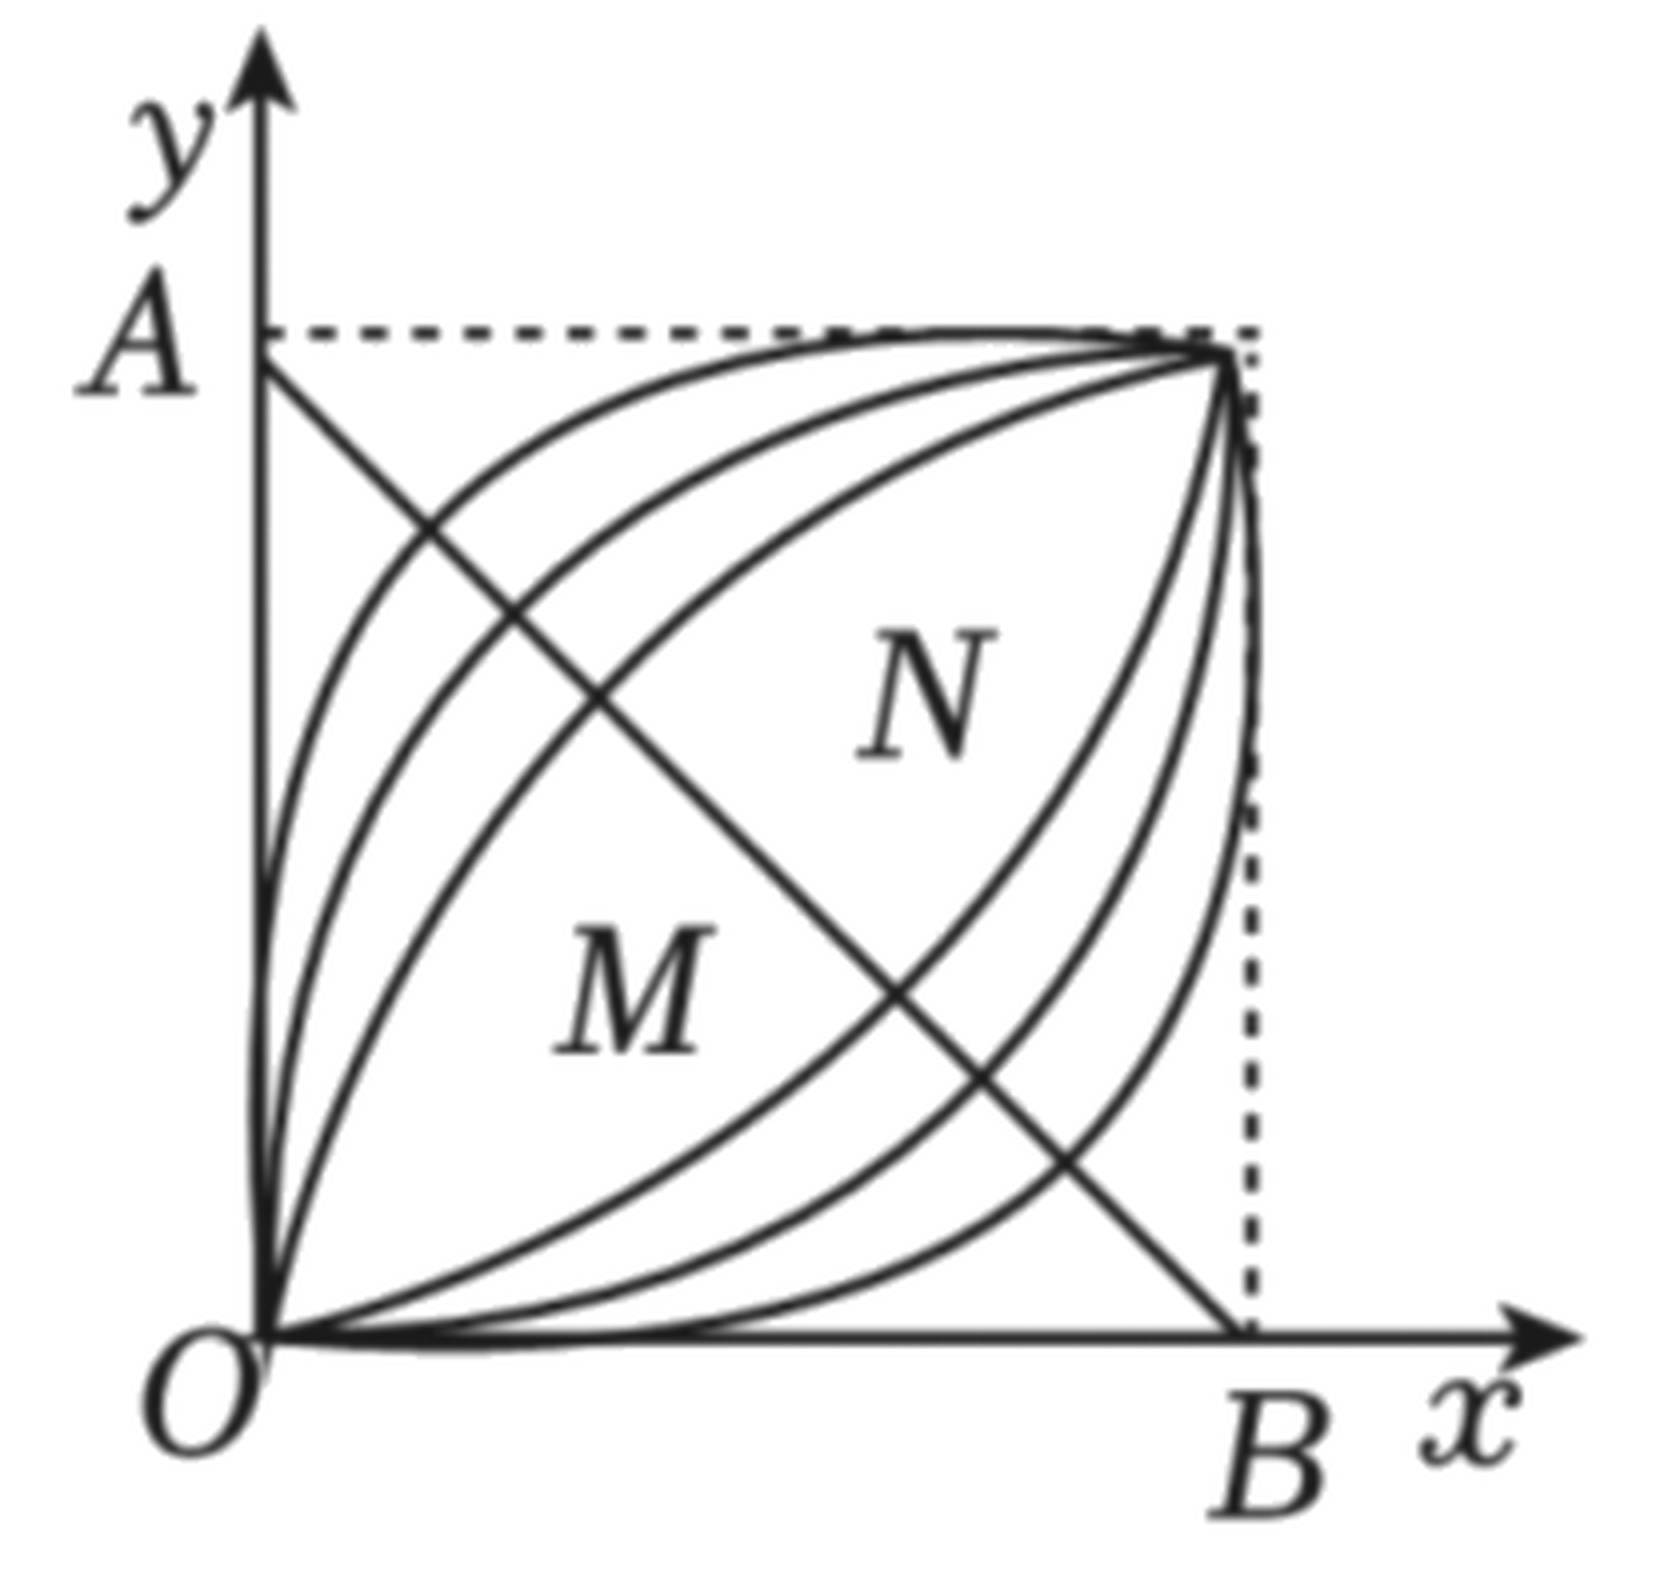
\includegraphics[width=0.40\textwidth]{figures/gao148_q12.png}
\end{center}

\ifanswer
\solbegin
\step{$BM=MN=NA$，点 $A(1,0)$，$B(0,1)$，所以 $M\left(\dfrac{1}{3},\dfrac{2}{3}\right)$，$N\left(\dfrac{2}{3},\dfrac{1}{3}\right)$，}
\step{分别代入 $y=x^\alpha$，$y=x^\beta$，$\alpha=\log_{\frac{2}{3}}\dfrac{1}{3},\beta=\log_{\frac{1}{3}}\dfrac{2}{3}$，$\alpha\beta=\log_{\frac{1}{3}}\dfrac{2}{3}\cdot\log_{\frac{2}{3}}\dfrac{1}{3}=1$.}
\solend
\fi

\end{enumerate}

\bigsec{二、选择题}

\begin{enumerate}
\setcounter{enumi}{12}

% === Q13 ===：答案"C"直接印在题干括号内、全卷无该题【答案】/【解析】段，按 高一84 Q13 成例括号留空、另提 \ans{$C$}；弯引号含空格
\item 若 $x$、$y\in\R$，则 “ $x=0$ ” 是 “ $xy=0$ ” 的\mbox{（\quad）}

\keepwithprev
A. 充要条件\qquad\qquad B. 必要不充分条件

C. 充分不必要条件\qquad\qquad D. 既不充分也不必要条件

\ifanswer
\ans{$C$}
\fi

% === Q14 ===：六个结论（圈数字在文本模式）、四选项一行；解析 8 行（对② 的两行公式各占一印刷行）
\item 若 $a<b<0$，下面有六个结论：① $a^2>b^2$；② $a^3<b^3$；③ $\dfrac{1}{a}<\dfrac{1}{b}$；④ $\dfrac{a}{b}>1$；⑤ $\dfrac{1}{a-b}>\dfrac{1}{a}$；⑥ $\lvert a\rvert>-b$. 其中正确的个数是\mbox{（\quad）}

\keepwithprev
A. 1\qquad\qquad B. 2\qquad\qquad C. 3\qquad\qquad D. 4

\ifanswer
\solbegin
\step{对①：$a^2-b^2=(a+b)(a-b),a+b<0,a-b<0$，故 $a^2-b^2>0$，正确；}
\step{对②：$a^3-b^3=(a-b)(a^2+ab+b^2)=(a-b)\left[\left(a+\dfrac{1}{2}b\right)^2+\dfrac{3}{4}b^2\right],a-b<0$，}
\step{$\left(a+\dfrac{1}{2}b\right)^2+\dfrac{3}{4}b^2>0$，故 $a^3-b^3<0$，正确；}
\step{对③：取 $a=-2,b=-1$，则 $\dfrac{1}{a}=-\dfrac{1}{2},\dfrac{1}{b}=-1,\dfrac{1}{a}>\dfrac{1}{b}$，错误；}
\step{对④：$\dfrac{a}{b}-1=\dfrac{a-b}{b},a-b<0,b<0$，故 $\dfrac{a}{b}-1>0$，正确；}
\step{对⑤：取 $a=-2,b=-1$，则 $\dfrac{1}{a-b}=-1,\dfrac{1}{a}=-\dfrac{1}{2},\dfrac{1}{a-b}<\dfrac{1}{a}$，错误；}
\step{对⑥：要证 $\lvert a\rvert>-b$，即 $-a>-b$，即 $a<b$，正确；}
\step{故选 $D$.}
\solend
\fi

% === Q15 ===：题目配图（四条指数函数曲线，三版都出），\needvspace 守卫放 \item 之前；"图象"照录；解析 5 行
\needvspace{8cm}
\item 如图，曲线①②③④分别是指数函数 $y=a^x$，$y=b^x$，$y=c^x$，$y=d^x$ 的图象，则实数 $a$、$b$、$c$、$d$ 的大小关系为\mbox{（\quad）}

\keepwithprev
A. $a<b<c<d$\qquad B. $b<a<d<c$\qquad C. $d<c<b<a$\qquad D. $c<d<a<b$

\begin{center}
% 四条指数函数曲线图取 04 页右侧，去粉色水印、去色、4× LANCZOS 放大；三版都出
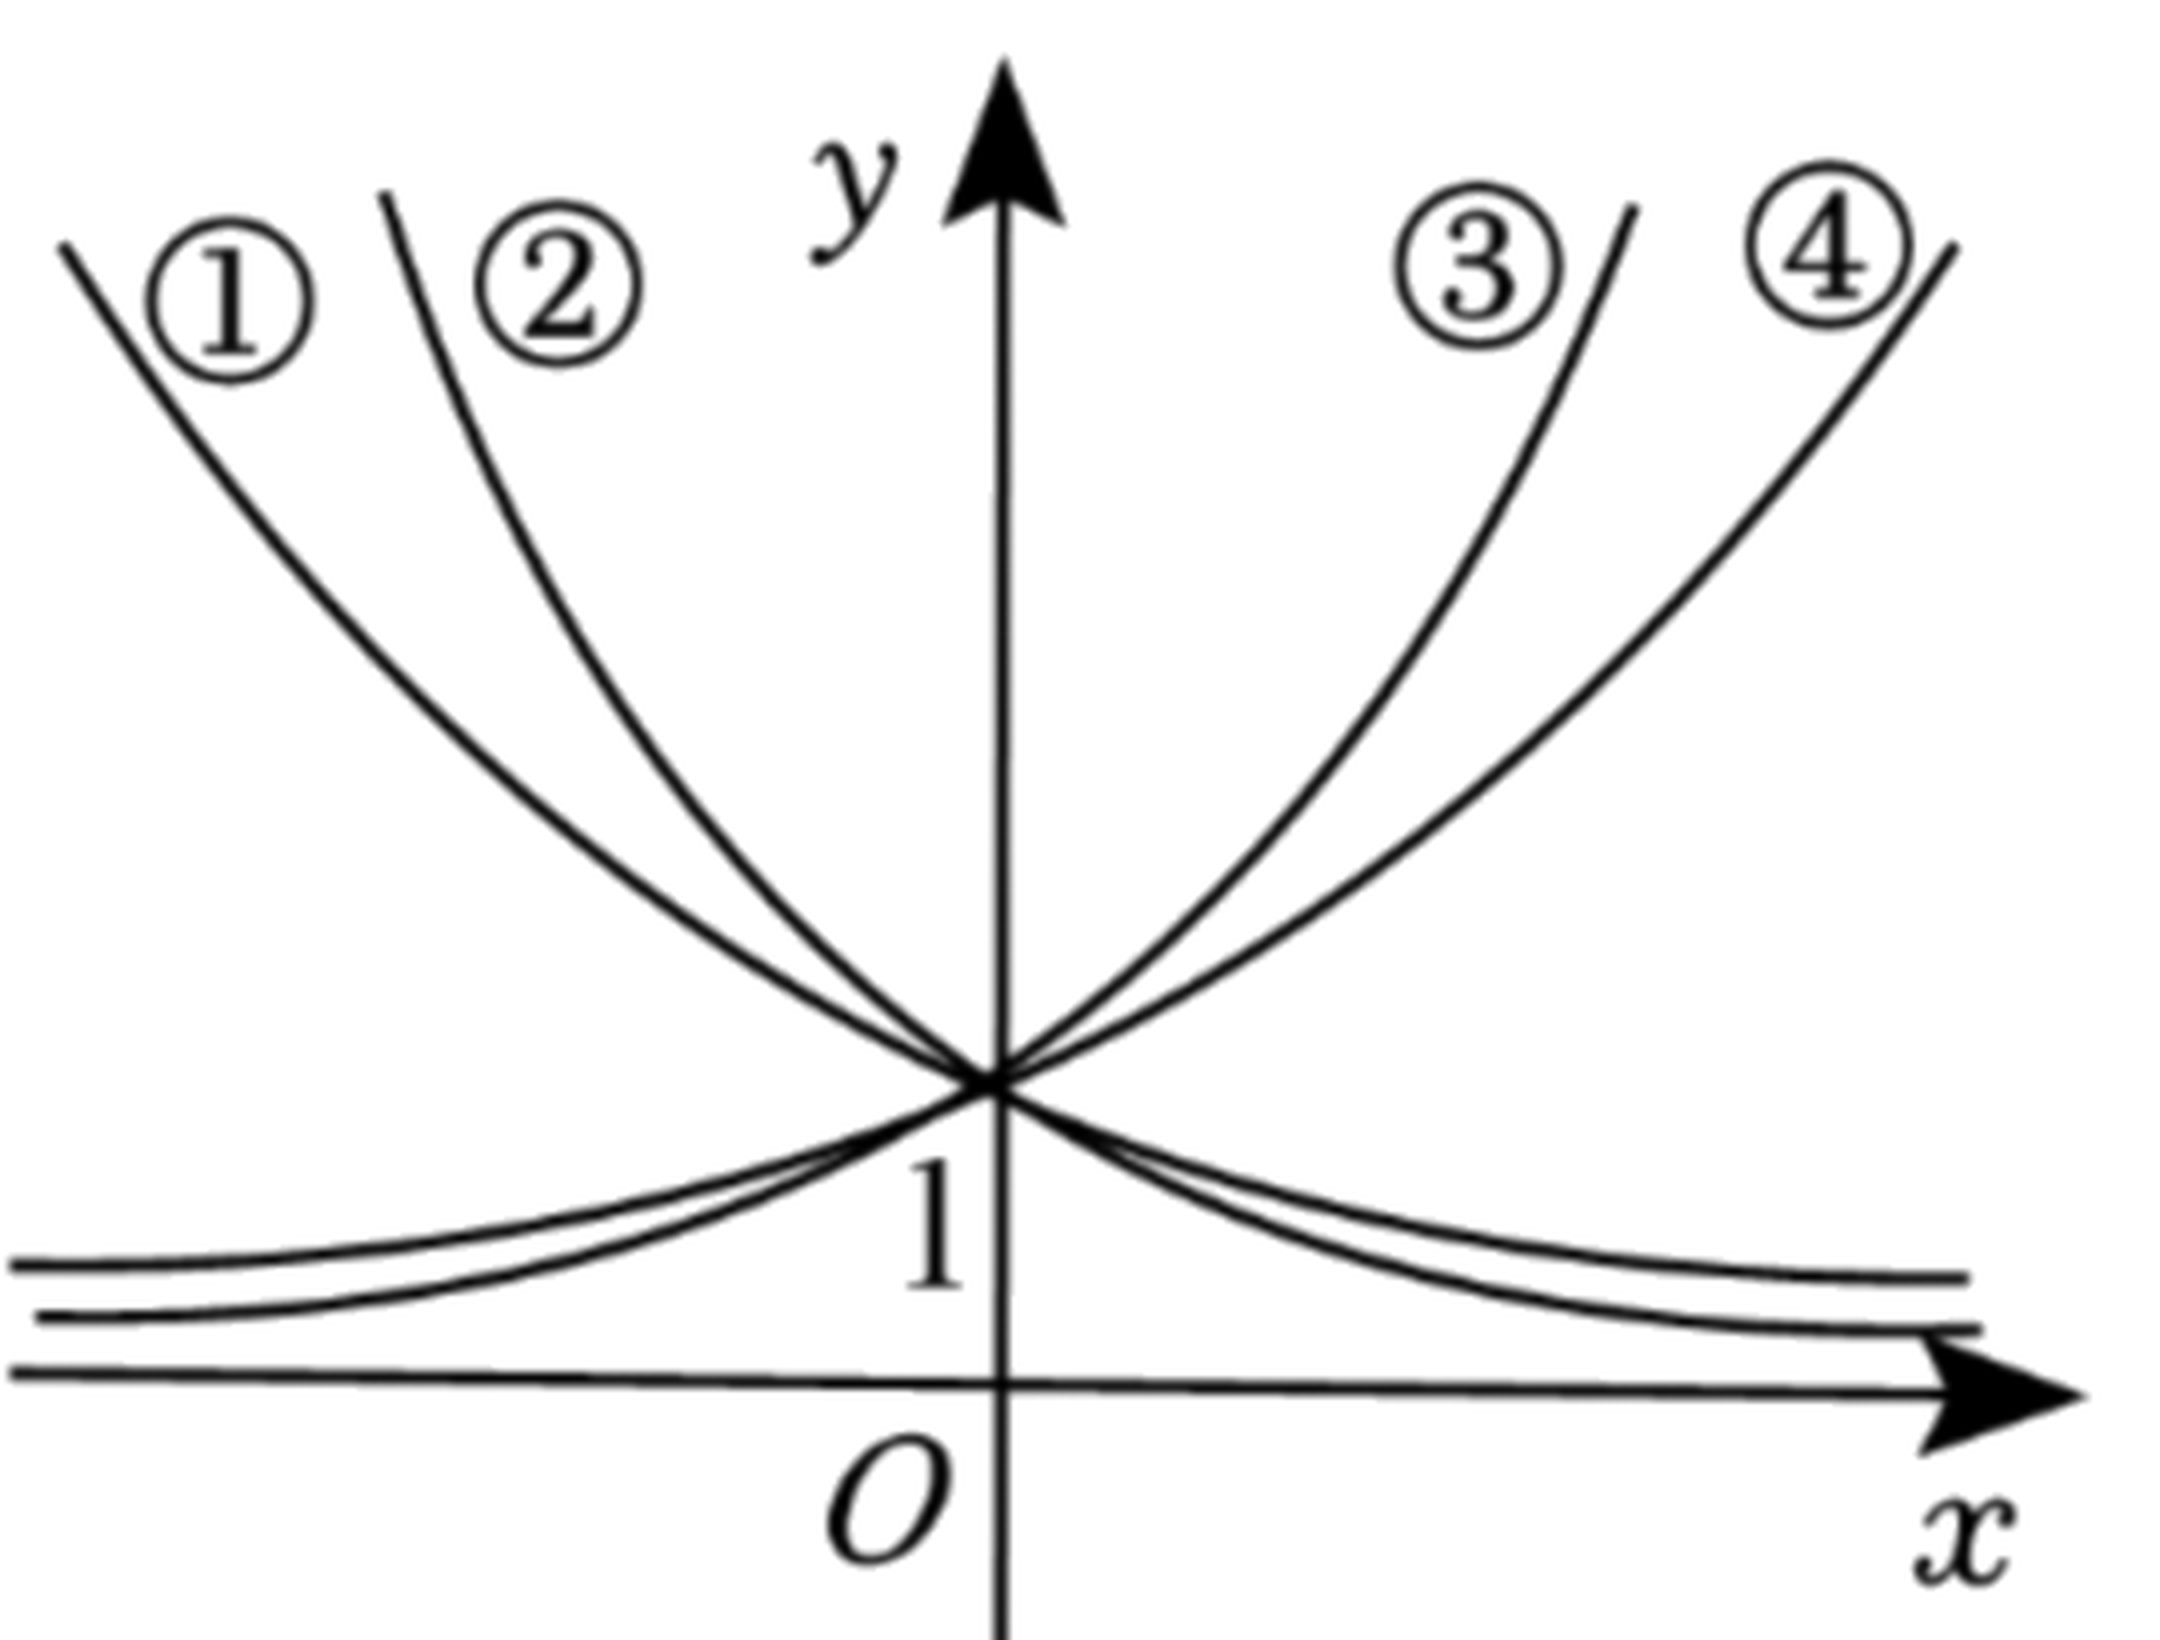
\includegraphics[width=0.40\textwidth]{figures/gao148_q15.png}
\end{center}

\ifanswer
\solbegin
\step{由函数图象得函数① $y=a^x$；② $y=b^x$ 为减函数，且 $x=1$ 时，$b^1<a^1$，}
\step{所以 $0<b<a<1$，}
\step{由函数图象得函数③ $y=c^x$；④ $y=d^x$ 为增函数，且 $x=1$ 时，$c^1>d^1$，}
\step{所以 $c>d>1$，}
\step{所以 $b<a<d<c$. 故选 $B$.}
\solend
\fi

% === Q16 ===：题目配图（关于 y 轴对称的幂函数曲线，三版都出），\needvspace 守卫放 \item 之前；$p$、$q\in\Z$；"图象"照录；解析 2 行
\needvspace{8cm}
\item 已知幂函数 $y=x^{\frac{p}{q}}$（$p$、$q\in\Z$ 且 $p$、$q$ 互质）的图象关于 $y$ 轴对称，如图所示，则\mbox{（\quad）}

\keepwithprev
A. $p$、$q$ 均为奇数，且 $\dfrac{p}{q}>0$\qquad\qquad B. $q$ 为偶数，$p$ 为奇数，且 $\dfrac{p}{q}<0$

C. $q$ 为奇数，$p$ 为偶数，且 $\dfrac{p}{q}>0$\qquad\qquad D. $q$ 为奇数，$p$ 为偶数，且 $\dfrac{p}{q}<0$

\begin{center}
% 关于 y 轴对称的幂函数曲线图取 04 页右下，去粉色水印、去色、4× LANCZOS 放大；三版都出
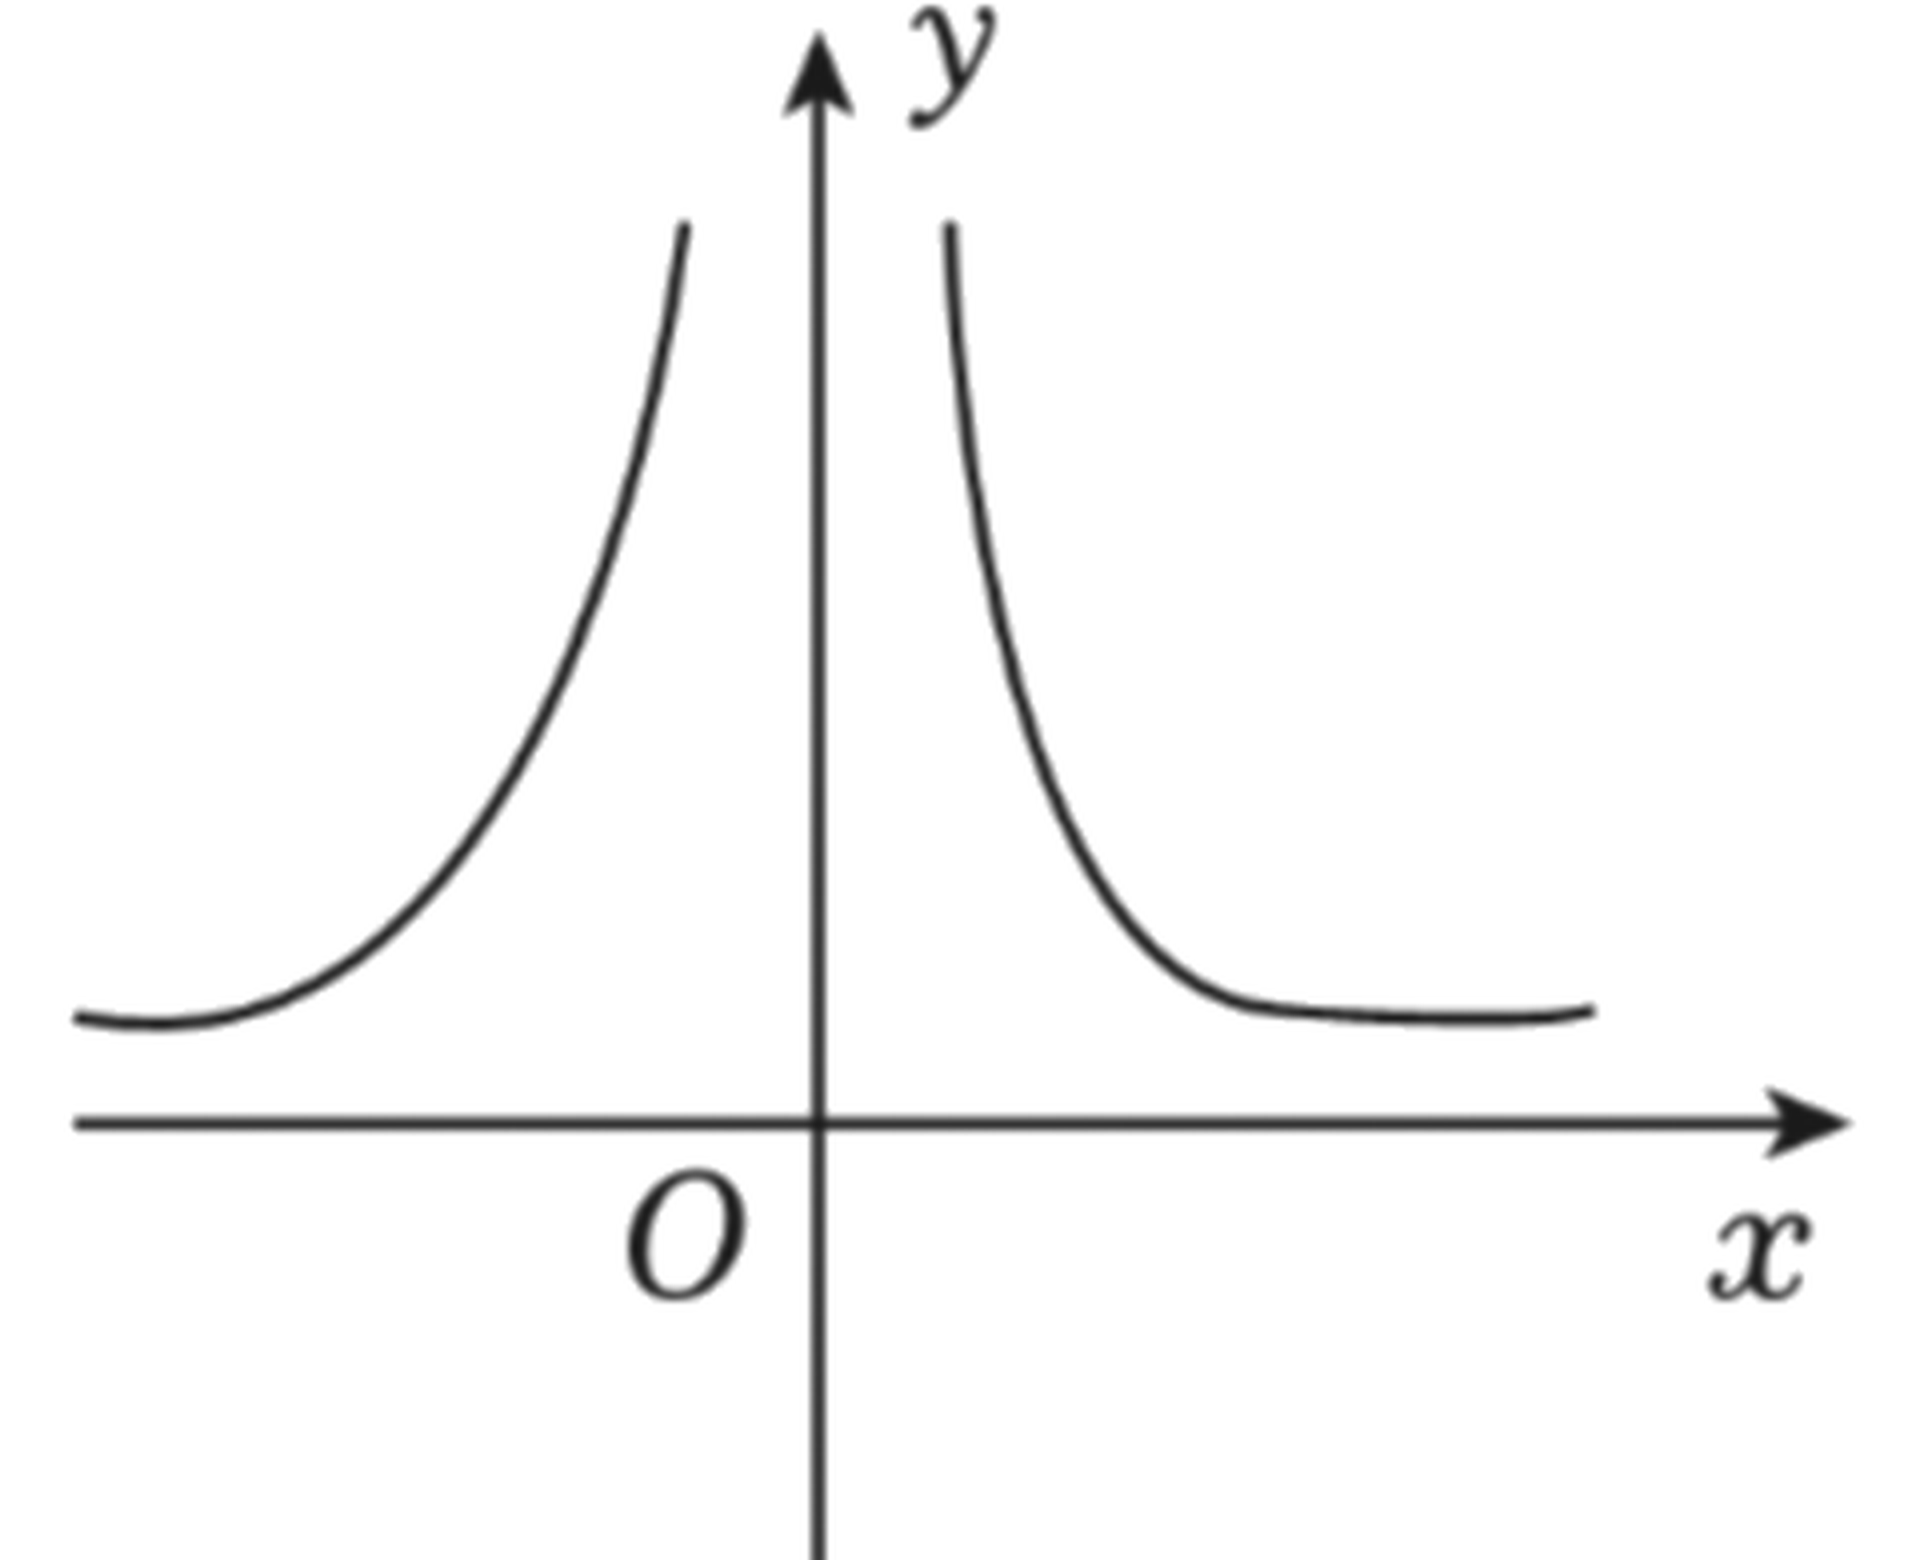
\includegraphics[width=0.36\textwidth]{figures/gao148_q16.png}
\end{center}

\ifanswer
\solbegin
\step{因为函数为偶函数，所以 $p$ 为偶数，且由图象形状判定 $\dfrac{p}{q}<0$.}
\step{又 $p$、$q$ 互质，所以 $q$ 为奇数. 故选 $D$.}
\solend
\fi

\end{enumerate}

\bigsec{三、解答题}

\begin{enumerate}
\setcounter{enumi}{16}

% === Q17 ===：\overline{B}／\varnothing／\R／\mid 逐处照录；解析 8 行
\item 已知集合 $A=\left\{x\mid \dfrac{5}{2x+1}>1\right\}$，$B=\{x\mid x^2+(a+3)x+3a<0,a\in\R\}$.

(1) 求 $A$.

(2) 若全集 $U=\R$，且 $A\cap\overline{B}=\varnothing$，求实数 $a$ 的取值范围.

\ifanswer
\solbegin
\step{(1) $\dfrac{5}{2x+1}>1$，即 $\dfrac{5}{2x+1}-1>0$，即 $\dfrac{4-2x}{2x+1}>0$，即 $(2x+1)(x-2)<0$，}
\step{解得 $-\dfrac{1}{2}<x<2$，所以 $A=\left(-\dfrac{1}{2},2\right)$；}
\step{(2) $x^2+(a+3)x+3a<0$，即 $(x+3)(x+a)<0$，}
\step{全集 $U=\R$，且 $A\cap\overline{B}=\varnothing$，}
\step{当 $a<3$ 时，解得 $-3<x<-a$，则 $\overline{B}=(-\infty,-3)\cup(-a,+\infty)$，}
\step{此时 $-a\geqslant2$，解得 $a\leqslant-2$，}
\step{当 $a\geqslant3$ 时，不满足 $A\cap\overline{B}=\varnothing$，}
\step{故实数 $a$ 的取值范围是 $(-\infty,-2]$.}
\solend
\fi

% === Q18 ===：cases 块整体算一个印刷行；解析 6 行
\item 已知幂函数经过点 $(2,4)$.

(1) 当 $x=\dfrac{1}{2}$ 时，求函数的值；

(2) 是否存在实数 $m$、$n$，使得该函数在区间 $[m,n]$ 上最小值为 $6m-8$，最大值为 $6n-8$？若存在，求出 $m$、$n$ 的值，若不存在，请说明理由.

\ifanswer
\solbegin
\step{(1) 设幂函数的解析式是 $y=x^\alpha$，则 $2^\alpha=4$，解得 $\alpha=2$，}
\step{故 $f(x)=x^2$，$f\left(\dfrac{1}{2}\right)=\dfrac{1}{4}$；}
\step{(2) 因为 $f(x)\geqslant0$，所以 $6m-8\geqslant0$，$m\geqslant\dfrac{4}{3}$，}
\step{由函数 $f(x)$ 在 $(0,+\infty)$ 严格增，得函数 $f(x)$ 在 $(m,n)$ 严格增，}
\step{所以 $\begin{cases}f(m)=6m-8\\f(n)=6n-8\end{cases}$ 且 $m<n$，解得 $m=2$，$n=4$，}
\step{故存在 $m=2$，$n=4$ 满足题意.}
\solend
\fi

% === Q19 ===：7 处评分档照 高一54／64 成例排 \dots\dots N 分；判别式高 \Delta；解析 9 行
\item 已知方程 $x^2+6mx+9m-2=0$，且 $x_1,x_2$ 是方程的两个不同的实数根.

(1) 若 $m=1$，求 $\dfrac{1}{x_1}+\dfrac{1}{x_2}$ 的值；

(2) 若 $m\in\R$，且 $x_1^2+x_2^2<4$，求 $m$ 取值范围.

\ifanswer
\solbegin
\step{(1) 当 $m=1$ 时，方程为 $x^2+6x+7=0$，\dots\dots1 分}
\step{则 $x_1+x_2=-6,x_1\cdot x_2=7$，\dots\dots2 分}
\step{$\dfrac{1}{x_1}+\dfrac{1}{x_2}=\dfrac{x_1+x_2}{x_1\cdot x_2}=-\dfrac{6}{7}$\dots\dots3 分}
\step{(2) $x_1+x_2=-6m,x_1\cdot x_2=9m-2$\dots\dots2 分}
\step{因为 $x_1^2+x_2^2=(x_1+x_2)^2-2x_1\cdot x_2$，所以 $(x_1+x_2)^2-2x_1\cdot x_2<4$，}
\step{所以 $36m^2-2(9m-2)<4$，解得 $0<m<\dfrac{1}{2}$\dots\dots2 分}
\step{又因为方程有两个不同的根，所以 $\Delta=36m^2-4(9m-2)>0$，}% 判别式原卷印等腰偏高粗三角 $\Delta$，照录（放大 07 页 q19_delta3.png／diag_band_q19.png 确认）
\step{解得 $m<\dfrac{1}{3}$ 或 $m>\dfrac{2}{3}$\dots\dots2 分}
\step{所以 $0<m<\dfrac{1}{3}$\dots\dots2 分}
\solend
\fi

% === Q20 ===：题目配图（矩形蔬菜温室，三版都出），\needvspace 守卫放 \item 之前；单位 \mathrm{m}／\mathrm{m}^2；解析 10 行
\needvspace{8cm}
\item 某村计划建造一个室内面积为 $600\mathrm{m}^2$ 的矩形蔬菜温室，在室内，沿左、右两侧与后侧内墙各保留 $2\mathrm{m}$ 宽的通道，沿前侧内墙保留 $4\mathrm{m}$ 宽的空地.

\begin{center}
% 矩形蔬菜温室示意图取 07 页右侧，去粉色水印、去色、4× LANCZOS 放大；三版都出
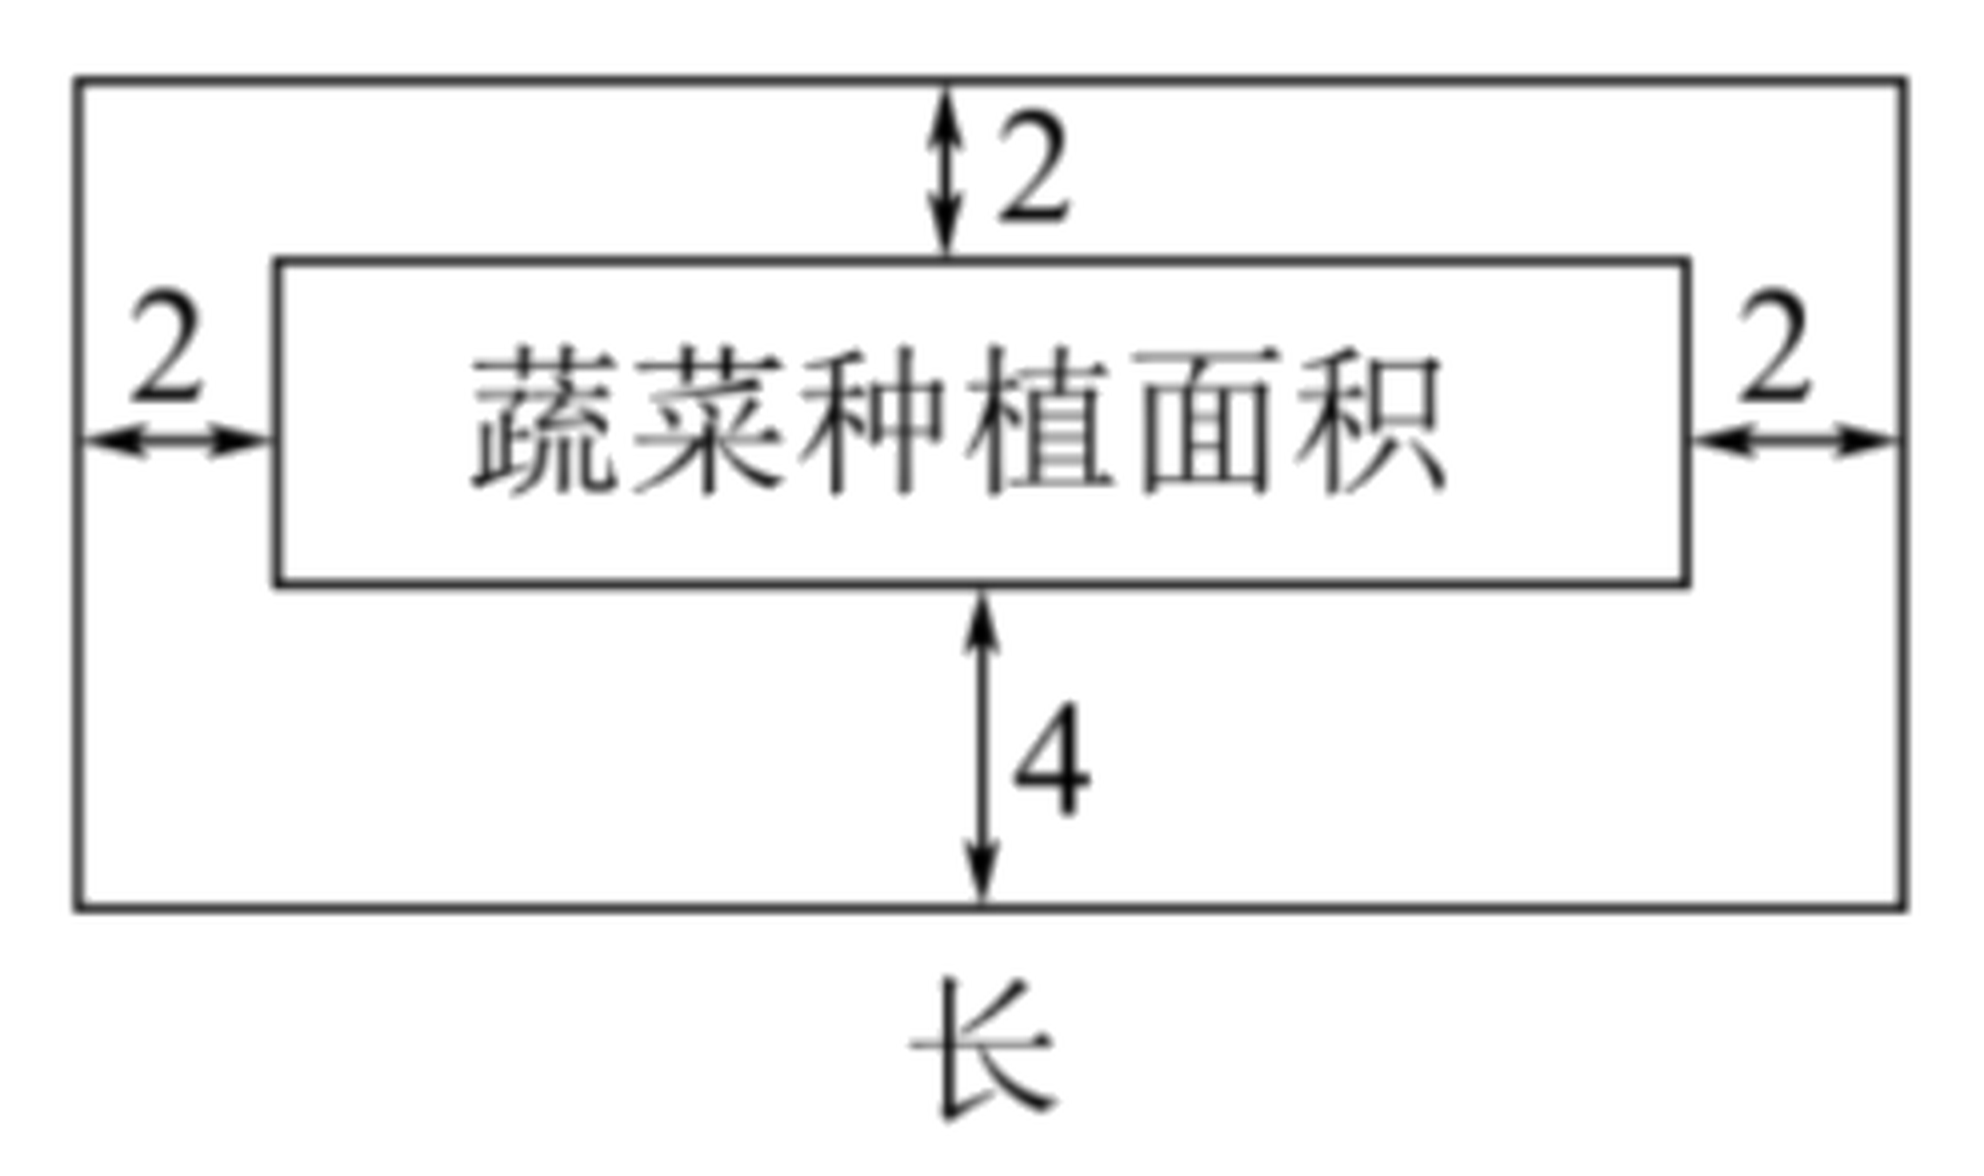
\includegraphics[width=0.45\textwidth]{figures/gao148_q20.png}
\end{center}

(1) 写出蔬菜的种植面积关于矩形温室的长之间的关系式.

(2) 当矩形温室的边长各为多少时，蔬菜的种植面积最大？最大种植面积是多少？

\ifanswer
\solbegin
\step{(1) 设蔬菜的种植面积为 $y\mathrm{m}^2$，矩形温室的长为 $x\mathrm{m}$，}
\step{则矩形温室的宽为 $\dfrac{600}{x}\mathrm{m}$，}
\step{种植蔬菜矩形的长为 $(x-4)\mathrm{m}$，宽为 $\left(\dfrac{600}{x}-6\right)\mathrm{m}$，}
\step{所以 $y=(x-4)\left(\dfrac{600}{x}-6\right)(4<x<100)$；}
\step{(2) 因为 $y=(x-4)\left(\dfrac{600}{x}-6\right)=624-\left(6x+\dfrac{2400}{x}\right)$，}
\step{因为 $6x+\dfrac{2400}{x}\geqslant2\sqrt{6x\cdot\dfrac{2400}{x}}=240$，}
\step{当且仅当 $6x=\dfrac{2400}{x}$，即 $x=20$ 时取等号，}
\step{所以 $y=624-\left(6x+\dfrac{2400}{x}\right)\leqslant624-240=384$.}
\step{即当矩形温室的一边长为 $20\mathrm{m}$，另一边长为 $30\mathrm{m}$ 时，}
\step{蔬菜的种植面积最大，最大为 $384\mathrm{m}^2$.}
\solend
\fi

% === Q21 ===：3 问、cases 块整体算一个印刷行；判别式高 \Delta；解析 19 行（末行续 09 页）
\item 二次函数 $f(x)=ax^2+bx+c$ 满足对任意的 $x\in\R$，$x-1\leqslant f(x)\leqslant x^2-x$ 恒成立.

(1) 求证：$f(1)$ 为定值；

(2) 若 $f(0)=-\dfrac{1}{4}$，求二次函数 $f(x)$ 的表达式；

(3) 求 $a+2b+5c$ 的取值范围.

\ifanswer
\solbegin
\step{(1) 对任意的 $x\in\R$，$x-1\leqslant f(x)\leqslant x^2-x$ 恒成立，则 $0\leqslant f(1)\leqslant0$，}
\step{所以 $f(1)=0$，为定值.}
\step{(2) 由(1)得 $a+b+c=f(1)=0$，由 $f(0)=-\dfrac{1}{4}$，得 $c=-\dfrac{1}{4}$，}
\step{则 $b=\dfrac{1}{4}-a$，$f(x)=ax^2+\left(\dfrac{1}{4}-a\right)x-\dfrac{1}{4}$，}
\step{不等式 $x-1\leqslant f(x)$ 可化为 $ax^2+\left(\dfrac{1}{4}-a\right)x-\dfrac{1}{4}\geqslant x-1$，}
\step{即 $ax^2-\left(a+\dfrac{3}{4}\right)x+\dfrac{3}{4}\geqslant0$，}
\step{一元二次不等式 $ax^2-\left(\dfrac{3}{4}+a\right)x+\dfrac{3}{4}\geqslant0$ 恒成立，则 $\begin{cases}a>0\\\Delta=\left(a+\dfrac{3}{4}\right)^2-3a\leqslant0\end{cases}$，}% 判别式原卷印等腰偏高粗三角 $\Delta$，照录（放大 08 页 q21_delta3.png／diag_band_q21.png 确认）
\step{解得 $a=\dfrac{3}{4}$，}
\step{此时 $f(x)=\dfrac{3}{4}x^2-\dfrac{1}{2}x-\dfrac{1}{4}$，$x^2-x-f(x)=\dfrac{1}{4}(x-1)^2\geqslant0$ 恒成立，}
\step{所以 $f(x)=\dfrac{3}{4}x^2-\dfrac{1}{2}x-\dfrac{1}{4}$.}
\step{(3) 由(1)得 $b=-a-c$，$f(x)=ax^2-(a+c)x+c=(ax-c)(x-1)$，}
\step{不等式 $x-1\leqslant f(x)$ 可化为 $(x-1)(ax-c-1)\geqslant0$，}
\step{一元二次不等式 $(x-1)(ax-c-1)\geqslant0$ 恒成立，则 $a>0$，}
\step{且方程 $(x-1)(ax-c-1)=0$ 有相等的实数根，因此 $c=a-1$，$a>0$，}
\step{不等式 $f(x)\leqslant x^2-x\Leftrightarrow(ax-c)(x-1)\leqslant x^2-x\Leftrightarrow(x-1)[(1-a)x+c]\geqslant0$，}
\step{同理 $1-a>0$，且方程 $(x-1)[(1-a)x+c]=0$ 有相等的实数根，}
\step{因此 $c=a-1$，$a<1$，从而 $c=a-1$，$b=1-2a$，$0<a<1$，}
\step{$a+2b+5c=a+2(1-2a)+5(a-1)=2a-3\in(-3,-1)$，}
\step{所以 $a+2b+5c$ 的取值范围是 $(-3,-1)$.}
\solend
\fi

\end{enumerate}

\end{document}
"
% 紧凑版：xelatex "\def\iscompact{1}% 高一148_新川中学_期中.tex
%   —— 高一上数学"2026-2027 年新川中学高一上期中"（试卷版/答案版/紧凑版）
% 试卷版：xelatex 高一148_新川中学_期中.tex
% 答案版：xelatex "\def\isanswer{1}\input{高一148_新川中学_期中.tex}"
% 紧凑版：xelatex "\def\iscompact{1}\input{高一148_新川中学_期中.tex}"
%
% ① 原始材料：微信公众号"魔都数学加油站"文章，连载"27学年高一148"，原文标题
% "27学年高一148——2026-2027年上海市新川中学高一上期中"（2026-11-21 推送）；
% 原文链接：https://mp.weixin.qq.com/s/Alhmwb3sSLQMp_wjzoAVyA 。
% 正文为 9 张 PNG 页（01/03/04/07/08/09 为 2560×3620，02/05/06 为 4762×6735，
% 同一篇各页分辨率混排，逐页按各自分辨率裁图核对，别按预览比例换算裁框）。
% 体例：混合体例讲评版——19 题中 Q4、Q5 只印【答案】、无【解析】；Q13 的答案"C"
% 直接印在题干括号内、无【答案】/【解析】段；其余 16 题印【解析】（逐题核实，见 ② ②）。
% 题目、答案、解析均据原图转录；卷面粉红色水印"魔都数学加油站"及公众号页脚未录入。
% 全卷插图清单（逐页通读 9 页确认）：4 幅题目配图，均三版都出、均非【解析】内配图：
%   · Q12 幂函数曲线族图（03 页右侧：x/y 轴、O、A(1,0)、B(0,1)、M、N 与两族
%     y=x^α／y=x^β 曲线、线段 AB、虚线），题干"（如图）"处，裁 figures/gao148_q12.png；
%   · Q15 四条指数函数曲线图（04 页右侧：①②③④ 四曲线同过 (0,1)、x/y 轴、O、
%     y 轴刻度 1），题干"如图"处，裁 figures/gao148_q15.png；
%   · Q16 关于 y 轴对称的幂函数曲线图（04 页右下：x/y 轴、O、两支上翘曲线），
%     题干"如图所示"处，裁 figures/gao148_q16.png；
%   · Q20 矩形蔬菜温室示意图（07 页右侧：大矩形＋内框"蔬菜种植面积"＋2/2/4
%     通道标注＋"长"），题干处，裁 figures/gao148_q20.png；
%   其余各页逐页确认无其它题目配图、无【解析】内配图、无表格，亦无"题干写如图而
%   源码漏图"一处；Q19 解析行末的虚线"----N 分"为评分档（非图），Q18／Q21 的
%   cases 块为数学块（非图）。4 图均取自原卷截图，去粉色水印、去色、4× LANCZOS 放大。
%
% 卷首标题：原卷印作"2026-2027 年新川中学高一上期中"，年份区间按全稿惯例排 en dash；
% 原卷卷面未印副标题，本稿按同期中卷（高一140／141／143／144／145／146／147）知识模块
% 口径补出"集合与常用逻辑用语、不等式、函数"。
%
% 题号体例（逐页核实定稿）：本卷共 19 题——一、填空题 3—12（10 题）、
% 二、选择题 13—16（4 题）、三、解答题 17—21（5 题）。
% 三节分别 \setcounter{enumi}{2}／{12}／{16}。原卷从第 3 题起、无第 1、2 题，
% 本稿保留原题号；全卷无附加题节、无 Q22（Q21 解析末行"所以 a+2b+5c 的取值范围是
% (-3,-1)."为全卷收尾，09 页下半仅水印、无正文）。
%
% ② 与原卷的排版差异：
%   ① 原文从第 3 题起，本稿保留原题号；共 19 题三节；
%   ② 混合体例逐题核实：Q4（反证法"假设的内容"）、Q5 只印【答案】、无【解析】，
%      按 高一140 第 5 题／高一145 Q3 成例提 \ans{}、不补造解析；Q13 答案"C"直接
%      印在题干括号内（" ( C ) "）、全卷无该题【答案】/【解析】段，按 高一84 Q13／
%      高一37 Q13／高一53 Q13 成例括号 \mbox{（\quad）} 留空、另提 \ans{$C$}；
%      其余 16 题印【解析】、用 \solbegin…\solend，选择题答案在解析末句"故选 X"
%      （Q14 选 D、Q15 选 B、Q16 选 D，逐个放大原图核实）、题干括号留空、不另提
%      \ans{}；答案版【答案】/【解析】标记数 = 19（3 个 \ans ＋ 16 个 \solbegin）
%      = 全卷题数；
%   ③ 原卷卷面未印副标题，本稿按知识模块口径补出；
%   ④ 原卷填空横线按全稿惯例排 \blankline[4.4em]；选择题括号排 \mbox{（\quad）}、
%      选项段前按惯例加 \keepwithprev；Q13／Q16 四选项为两行两列、Q14／Q15 选项
%      为一行，照原卷分行；解答题不留作答区、不加 \anspace（原卷为讲评版，
%      与 129／131／132／133／136／140／141／143／144／145／146 同）；
%   ⑤ 数集：Q11"在 R 上定义运算"、Q13"x、y∈R"、Q16"p、q∈Z"、Q17"a∈R"
%      "U=R"、Q19"m∈R"、Q21"x∈R" 原卷印斜体 R/Z，按全稿惯例统一改 \R／\Z
%      （本卷未出现 N，\N^* 无对应处）；绝对值排 \lvert…\rvert（Q9／Q14），
%      集合描述竖线排 \mid（Q17）；不等号按全稿惯例排 \leqslant／\geqslant；
%      补集照原卷上划线排 \overline{B}（Q17 题干 1 处＋解析 3 处）；空集
%      \varnothing（Q17 题干 1 处＋解析 2 处）；\subset（Q3 题干 {a}⊂M）与
%      \subseteq（Q3 题干 M⊆{a,b,c,d}）逐处照录不统一（放大 01 页 q3_subset.png）；
%   ⑥ 子题标号 (1)(2)(3) 半角括号照录；圈数字 ①—⑥ 在文本模式（Q14 六个结论、
%      Q15 曲线编号与其解析、Q14 解析"对①…对⑥"），按 common.sty 划入 CJK 字符类
%      渲染；cases 块整体算一个印刷行；\left…\right 不得拆到不同 $…$ 组；
%      单位 m／m² 排 \mathrm{m}／\mathrm{m}^2（Q20，原卷印正体 m）；
%   ⑦ 题干／解析中的中文弯引号按原卷照录：Q4" ab 可以被 5 整除，那么 a、b 中
%      至少有一个能被 5 整除 "（开引号后有空格、闭引号后空格接"时"）、
%      Q13" x=0 "" xy=0 "（引号内空格），注释内一律 ASCII 引号；
%   ⑧ 半角逗号在数学组之间是全稿惯例、非笔误（Q3"{a,b,c,d}"、Q6"$x,y$"
%      "$x=\frac13,y=\frac16$"、Q10、Q11"$a=-2,b=-1"、Q12"$\alpha=\log..,\beta=..$"、
%      Q14"$a+b<0,a-b<0$"、Q17、Q19"$x_1+x_2=-6,x_1\cdot x_2=7$"、Q20、Q21 等），
%      逐处照录别改全角；行末西文句点照录为 ASCII `.`；行中全角逗号／顿号照录；
%   ⑨ "图像／图象"逐处放大核：全卷 9 处均印"图象"（象，无亻）、未见"图像"，
%      逐处照录未统一改动（Q8 题干/解析各 1、Q12 题干 2、Q15 题干 1／解析 2、
%      Q16 题干 1／解析 1；放大 02/03/04/05 页 /tmp/gao148/zoom/my_wide_a.png、
%      my_wide_b.png 与宋体参考"象／像"并排确认）；
%   ⑩ 判别式 Δ/△ 混用是照录项：Q11 解析"△=1−4(−a²+a+1)<0"印扁等边空心
%      三角 \triangle；Q19 解析"Δ=36m²−4(9m−2)>0"、Q21 解析 cases 块
%      "Δ=(a+3/4)²−3a≤0" 两处印等腰偏高粗三角 \Delta，逐处放大判断、照录
%      不统一（参照 高一142／144／145 头注④口径，详见 ④）；
%   ⑪ 一条 \step = 原卷解析的一个印刷行，cases 块整体算一个印刷行；别把原卷折行
%      并起来、别把一行拆多条。Q3 六行、Q7 五行（01 页末首行＋02 页顶四行）、
%      Q9 七行、Q11 五行、Q14 八行（对② 的两行公式各占一印刷行）、Q17 八行、
%      Q18 六行、Q19 九行（7 处评分档附在行末）、Q20 十行、Q21 十九行
%      均按印刷行逐条断，不丢行；
%   ⑫ 配图：4 幅均为题目配图（三版都出），放 \item 内题干之后 \begin{center}；
%      大图块加 \needvspace 守卫把整块推走（守卫放 \item 之前，见 高一145 Q14/Q20
%      成例与切页审计 B 类坑）；三版切页审计均"合计异常：无"；
%   ⑬ 跨页续印按题合并：Q3/4/5 在 01 页；Q6 题干＋解析在 01 页；Q7 题干在 01 页
%      末、解析首行在 01 页末续 02 页顶四行；Q8/9/10 在 02 页（Q9 解析续 02 页下半、
%      Q10 题干与解析前 2 行在 02 页末）；Q10 解析末行续 03 页顶；Q11/12 在 03 页、
%      "二、选择题"标题与 Q13/14 题干在 03 页下半；Q13 无解析；Q14 解析在 04 页顶、
%      Q15 题干＋图＋选项＋解析在 04 页、Q16 题干＋图在 04 页末；Q16 选项＋解析＋
%      "三、解答题"标题＋Q17 题干＋解析在 05 页、Q18 题干首句在 05 页末；Q18 题干
%      续＋解析、Q19 题干＋解析前 5 行在 06 页；Q19 解析续 4 行＋Q20 题干＋图＋
%      解析（10 行全部）在 07 页，末行"蔬菜的种植面积最大，最大为 384m²."收尾；
%      Q21 题干＋解析前 18 行在 08 页；Q21 解析末行"所以 a+2b+5c 的取值范围是
%      (-3,-1)."在 09 页上半（09 页下半仅水印、无正文）。本稿按题连排，不丢行、
%      不并折行；
%   ⑭ 原卷解析内无红色"法一／法二"之类小标题，故本卷无 \stepm；水印
%      "魔都数学加油站"红色不录入；Q19 解析 7 处评分档（1/2/3/2/2/2/2 分）
%      原卷在行末印一串虚线，本稿照 高一54／64 成例排 \dots\dots N 分，
%      分值逐处照录、位置不变。
%
% ③ 行数复核：一条 \step／\stepm = 原卷解析的一个印刷行，cases 块作一个印刷行计。
%   逐题数（主会话逐页核对定稿）：Q3：6；Q4：0（只印【答案】、提 \ans{}）；
%   Q5：0（只印【答案】、提 \ans{}）；Q6：2；Q7：5；Q8：2；Q9：7；Q10：3；
%   Q11：5；Q12：2；Q13：0（答案印在题干括号内、另提 \ans{}）；Q14：8；Q15：5；
%   Q16：2；Q17：8；Q18：6；Q19：9；Q20：10；Q21：19。
%   合计 99 条 \step（本卷无 \stepm：解析内无红色"法一／法二"类小标题），
%   与原卷逐题印刷行相等。全卷 16 题设 \solbegin…\solend ＋ 3 处 \ans{}，
%   答案版【答案】/【解析】标记数 = 19 = 全卷题数。
%
% ④ 判别式／子集符号结论（逐处放大原图照录、不得统一，主会话像素级复核）：
%   判别式全卷 3 处，两形混用逐处照录不统一（参照 高一142／144／145 头注④口径）：
%     · Q11 解析"△=1−4(−a²+a+1)<0" 原卷印扁等边空心三角（宽>高、细线），
%       照录 \triangle（放大 03 页 /tmp/gao148/zoom/q11_delta3.png、
%       delta_montage.png 确认）；
%     · Q19 解析"Δ=36m²−4(9m−2)>0" 原卷印等腰偏高粗三角（高>宽），
%       照录 \Delta（放大 07 页 /tmp/gao148/zoom/q19_delta3.png 确认）；
%     · Q21 解析 cases 块"Δ=(a+3/4)²−3a≤0" 原卷印等腰偏高粗三角（高>宽），
%       照录 \Delta（放大 08 页 /tmp/gao148/zoom/q21_delta3.png 确认）。
%   子集／补集：Q3 题干"{a}⊂M⊆{a,b,c,d}" 前者印单线 ⊂、无下划线，照录 \subset；
%     后者印带下划线 ⊆，照录 \subseteq（放大 01 页 /tmp/gao148/zoom/q3_subset.png
%     确认）；Q17 题干 1 处＋解析 3 处共 4 处 \overline{B} 照原卷上划线
%     （B 上横线、非 C_U B）；空集 \varnothing 3 处（Q17 题干 1 处、解析 2 处）；
%     Q17 集合描述竖线 \mid；数集 \R／\Z 归一见 ② ⑤。
%
% ⑤ 存疑照录（放大原图确认，照录未改、正文对应处另有 % 注）：
%   1. Q3 解析末行"所以 M 一共有 3+3+1+1=8 个" 原卷印 $3+3+1+1=8$，按上文
%      四行应为 $1+3+3+1=8$（疑为原卷加数顺序笔误，和仍为 8），放大 01 页
%      /tmp/gao148/zoom/my_q3_sol.png 确认，照录未改。
%   2. Q13 答案"C"直接印在题干括号内、全卷无该题【答案】/【解析】段，按
%      高一84 Q13 成例括号留空、另提 \ans{$C$}（见 ② ②），未补造解析。
%   3. Q19 解析 7 处评分档（"----N 分"）原卷印一串虚线，本稿照 高一54／64
%      成例排 \dots\dots N 分，分值逐处照录、位置不变。
%   4. 判别式 Q11 扁 \triangle 与 Q19／Q21 高 \Delta 两形混用，逐处照录不统一（见 ④）。
%   5. "图像／图象"全卷 9 处均印"图象"、未见"图像"（见 ② ⑨），逐处放大核实照录，
%      未统一改动。
%   全卷除此 5 类外未发现其它笔误／自相矛盾处。
%
% ⑥ 跨页续印按题合并说明：见 ② ⑬。
%
\documentclass[a4paper,11pt]{article}
\usepackage{common}

\begin{document}

\examtitlest[3]{2026--2027 年新川中学高一上期中}{集合与常用逻辑用语、不等式、函数}

\bigsec{一、填空题}

\begin{enumerate}
\setcounter{enumi}{2}

% === Q3 ===：题干 {a}⊂M⊆{a,b,c,d} 两个子集符号逐处照录；解析 6 行
\item 满足 $\{a\}\subset M\subseteq\{a,b,c,d\}$ 的集合 $M$ 有\blankline[4.4em]个.

\ifanswer
\solbegin
\step{$M$ 是 $\{a,b,c,d\}$ 的子集，但必含有元素 $a$，}
\step{当 $M$ 中只一个元素时，$M=\{a\}$ 只有 1 个；}
\step{当 $M$ 中有二个元素时，$M$ 有 3 个；}
\step{当 $M$ 中有三个元素时，$M$ 有 3 个；}
\step{当 $M$ 中有四个元素时，$M$ 有 1 个；}
\step{所以 $M$ 一共有 $3+3+1+1=8$ 个.}% 原卷印 $3+3+1+1=8$（按上文四行应为 $1+3+3+1$），疑为加数顺序笔误，照录未改（放大 01 页 my_q3_sol.png）
\solend
\fi

% === Q4 ===：原卷只印【答案】、无【解析】，按 高一140 第 5 题成例提 \ans{}；弯引号与空格照录
\item 用反证法证明命题 “ $ab$ 可以被 5 整除，那么 $a$、$b$ 中至少有一个能被 5 整除” 时假设的内容应该是\blankline[4.4em].

\ifanswer
\ans{$a$、$b$ 都不能被 5 整除}
\fi

% === Q5 ===：原卷只印【答案】 $[-2,1)$、无【解析】，提 \ans{}
\item 不等式 $\dfrac{x+2}{x-1}\leqslant0$ 的解集为\blankline[4.4em].

\ifanswer
\ans{$[-2,1)$}
\fi

% === Q6 ===：解析 2 行；半角逗号在数学组之间照录
\item 设 $x,y\in(0,+\infty)$，且 $x+4y=1$，则 $\dfrac{1}{x}+\dfrac{1}{y}$ 的最小值为\blankline[4.4em].

\ifanswer
\solbegin
\step{因为 $\dfrac{1}{x}+\dfrac{1}{y}=(x+4y)\left(\dfrac{1}{x}+\dfrac{1}{y}\right)=5+\dfrac{4y}{x}+\dfrac{x}{y}\geqslant5+2\sqrt{\dfrac{4y}{x}\cdot\dfrac{x}{y}}=9$，}
\step{当且仅当 $\dfrac{4y}{x}=\dfrac{x}{y}$，即 $x=2y$，即 $x=\dfrac{1}{3},y=\dfrac{1}{6}$ 时取等号，故最小值为 9.}
\solend
\fi

% === Q7 ===：题干在 01 页末、解析首行在 01 页末续 02 页顶四行；解析 5 行
\item 若不等式 $x^2+ax+b<0$ 的解集为 $(-3,-1)$，则不等式 $bx^2+ax+1\leqslant0$ 的解集为\blankline[4.4em].

\ifanswer
\solbegin
\step{不等式 $x^2+ax+b<0$ 的解集为 $(-3,-1)$，}
\step{所以方程 $x^2+ax+b=0$ 的两个实数根为 $-3$ 和 $-1$，}
\step{由根与系数的关系得 $a=4$，$b=3$，}
\step{故 $bx^2+ax+1\leqslant0$ 可化为 $3x^2+4x+1\leqslant0$，解得 $-1\leqslant x\leqslant-\dfrac{1}{3}$，}
\step{所求不等式 $bx^2+ax+1\leqslant0$ 的解集为 $\left[-1,-\dfrac{1}{3}\right]$.}
\solend
\fi

% === Q8 ===："图象"照录；解析 2 行
\item 函数 $y=a^{x-2}+2(a>0,a\ne1)$ 的图象必经过定点\blankline[4.4em].

\ifanswer
\solbegin
\step{令 $x-2=0$，得 $x=2$，则 $y=a^0+2=3$，}
\step{所以函数 $y=a^{x-2}+2$ 的图象过定点 $(2,3)$.}
\solend
\fi

% === Q9 ===：解析 7 行；首句末西文句点照录
\item 不等式 $\lvert x+3\rvert+\lvert a-x\rvert>6$ 对一切实数 $x$ 恒成立，则实数 $a$ 的取值范围为\blankline[4.4em].

\ifanswer
\solbegin
\step{$\lvert x+3\rvert$ 表示 $x$ 到 $-3$ 的距离，$\lvert a-x\rvert$ 表示 $x$ 到 $a$ 的距离.}
\step{所以它们的和为 $x$ 到 $-3$ 和 $x$ 到 $a$ 的距离之和，}
\step{当 $x$ 位于 $-3$ 和 $a$ 之间时，距离和取得最小值，}
\step{即两点之间的距离 $\lvert a-(-3)\rvert=\lvert a+3\rvert$，}
\step{若最小值 $\lvert a+3\rvert>6$，则原式对所有 $x$ 恒成立.}
\step{解得 $a+3>6$ 或 $a+3<-6$，即 $a>3$ 或 $a<-9$，}
\step{故 $a\in(3,+\infty)$ 或 $a\in(-\infty,-9)$.}
\solend
\fi

% === Q10 ===：题干与解析前 2 行在 02 页末、解析末行续 03 页顶；解析 3 行
\item 已知 $2^a=3$，$\log_3 5=b$，则 $\log_{15}20=$\blankline[4.4em]（用 $a$、$b$ 表示）.

\ifanswer
\solbegin
\step{因为 $2^a=3$，所以 $a=\log_2 3=\dfrac{\lg3}{\lg2}$，又 $\log_3 5=b=\dfrac{\lg5}{\lg3}$，}
\step{所以 $\lg3=a\lg2$，$\lg5=b\lg3=ba\lg2$，}
\step{则 $\log_{15}20=\dfrac{2\lg2+\lg5}{\lg3+\lg5}=\dfrac{2\lg2+ab\lg2}{a\lg2+ab\lg2}=\dfrac{2+ab}{a+ab}$.}
\solend
\fi

% === Q11 ===：在 \R 上定义运算 \otimes；判别式扁 \triangle 照录；解析 5 行
\item 在 $\R$ 上定义运算 $\otimes:x\otimes y=x(1-y)$，若不等式 $(x-a)\otimes(x+a)<1$ 对任意实数 $x$ 恒成立，则 $a$ 的取值范围是\blankline[4.4em].

\ifanswer
\solbegin
\step{由题意得不等式 $(x-a)\otimes(x+a)<1$ 对任意实数 $x$ 恒成立，}
\step{即不等式 $(x-a)(1-x-a)<1$ 对任意实数 $x$ 恒成立，}
\step{即 $x^2-x-a^2+a+1>0$ 对任意实数 $x$ 恒成立，}
\step{所以 $\triangle=1-4(-a^2+a+1)<0$，解得 $-\dfrac{1}{2}<a<\dfrac{3}{2}$，}% 判别式原卷印扁等边空心三角 $\triangle$，照录（放大 03 页 q11_delta3.png 确认）
\step{所以实数 $a$ 的取值范围为 $\left(-\dfrac{1}{2},\dfrac{3}{2}\right)$.}
\solend
\fi

% === Q12 ===：题目配图（幂函数曲线族，三版都出）；"图象"照录；解析 2 行
\needvspace{8cm}
\item 幂函数 $y=x^\alpha$，当 $\alpha$ 取不同的正数时，在区间 $[0,1]$ 上它们的图象是一族美丽的曲线（如图）. 设点 $A(1,0)$，$B(0,1)$，连接 $AB$，线段 $AB$ 恰好被其中的两个幂函数 $y=x^\alpha$，$y=x^\beta$ 的图象三等分，即有 $BM=MN=NA$，那么 $\alpha\beta=$\blankline[4.4em].

\begin{center}
% 幂函数曲线族图取 03 页右侧，去粉色水印、去色、4× LANCZOS 放大；三版都出
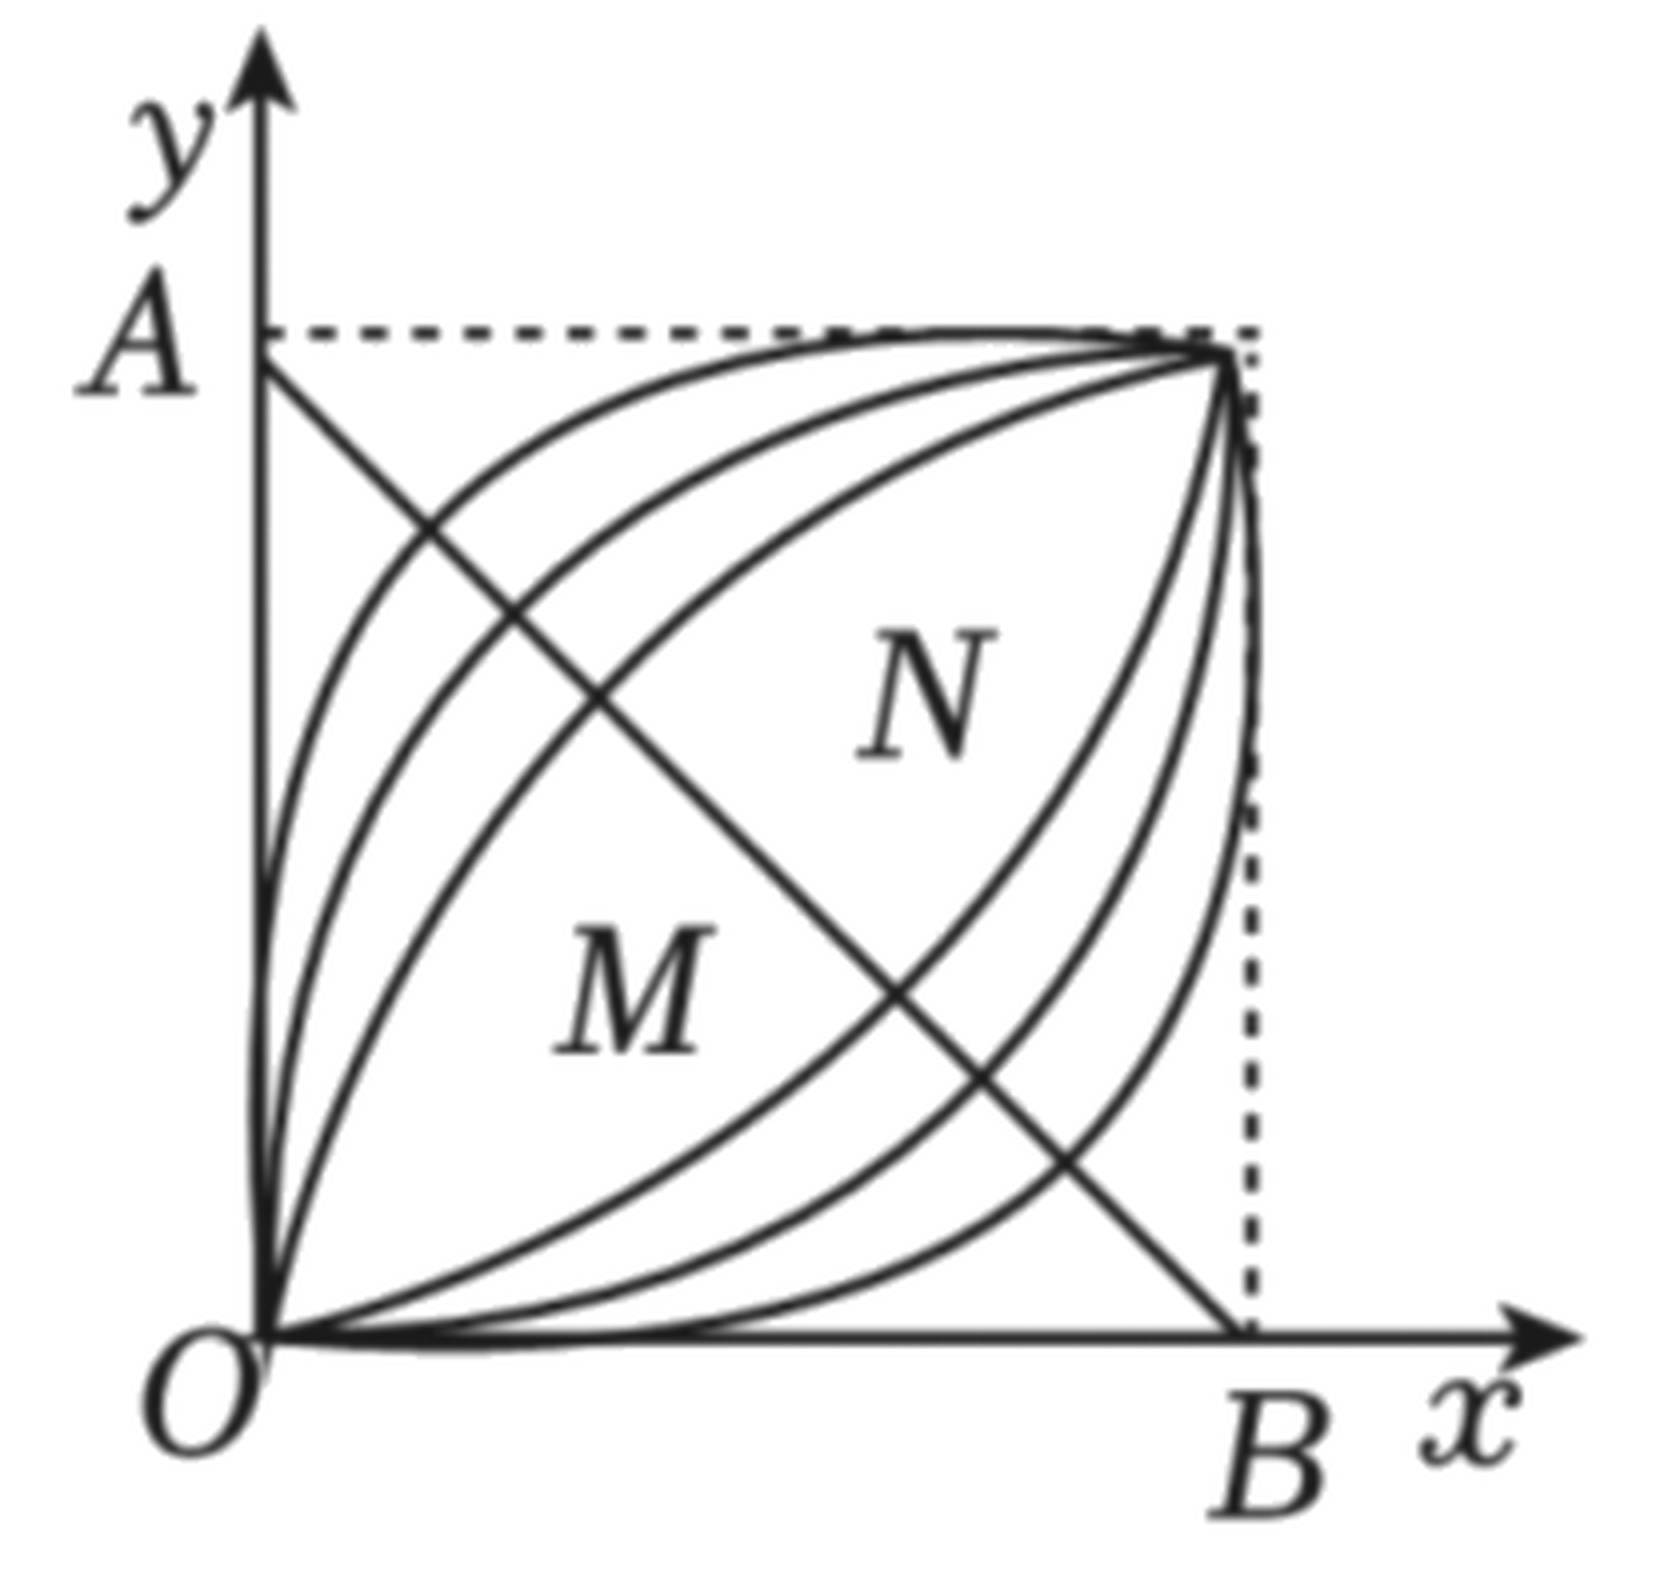
\includegraphics[width=0.40\textwidth]{figures/gao148_q12.png}
\end{center}

\ifanswer
\solbegin
\step{$BM=MN=NA$，点 $A(1,0)$，$B(0,1)$，所以 $M\left(\dfrac{1}{3},\dfrac{2}{3}\right)$，$N\left(\dfrac{2}{3},\dfrac{1}{3}\right)$，}
\step{分别代入 $y=x^\alpha$，$y=x^\beta$，$\alpha=\log_{\frac{2}{3}}\dfrac{1}{3},\beta=\log_{\frac{1}{3}}\dfrac{2}{3}$，$\alpha\beta=\log_{\frac{1}{3}}\dfrac{2}{3}\cdot\log_{\frac{2}{3}}\dfrac{1}{3}=1$.}
\solend
\fi

\end{enumerate}

\bigsec{二、选择题}

\begin{enumerate}
\setcounter{enumi}{12}

% === Q13 ===：答案"C"直接印在题干括号内、全卷无该题【答案】/【解析】段，按 高一84 Q13 成例括号留空、另提 \ans{$C$}；弯引号含空格
\item 若 $x$、$y\in\R$，则 “ $x=0$ ” 是 “ $xy=0$ ” 的\mbox{（\quad）}

\keepwithprev
A. 充要条件\qquad\qquad B. 必要不充分条件

C. 充分不必要条件\qquad\qquad D. 既不充分也不必要条件

\ifanswer
\ans{$C$}
\fi

% === Q14 ===：六个结论（圈数字在文本模式）、四选项一行；解析 8 行（对② 的两行公式各占一印刷行）
\item 若 $a<b<0$，下面有六个结论：① $a^2>b^2$；② $a^3<b^3$；③ $\dfrac{1}{a}<\dfrac{1}{b}$；④ $\dfrac{a}{b}>1$；⑤ $\dfrac{1}{a-b}>\dfrac{1}{a}$；⑥ $\lvert a\rvert>-b$. 其中正确的个数是\mbox{（\quad）}

\keepwithprev
A. 1\qquad\qquad B. 2\qquad\qquad C. 3\qquad\qquad D. 4

\ifanswer
\solbegin
\step{对①：$a^2-b^2=(a+b)(a-b),a+b<0,a-b<0$，故 $a^2-b^2>0$，正确；}
\step{对②：$a^3-b^3=(a-b)(a^2+ab+b^2)=(a-b)\left[\left(a+\dfrac{1}{2}b\right)^2+\dfrac{3}{4}b^2\right],a-b<0$，}
\step{$\left(a+\dfrac{1}{2}b\right)^2+\dfrac{3}{4}b^2>0$，故 $a^3-b^3<0$，正确；}
\step{对③：取 $a=-2,b=-1$，则 $\dfrac{1}{a}=-\dfrac{1}{2},\dfrac{1}{b}=-1,\dfrac{1}{a}>\dfrac{1}{b}$，错误；}
\step{对④：$\dfrac{a}{b}-1=\dfrac{a-b}{b},a-b<0,b<0$，故 $\dfrac{a}{b}-1>0$，正确；}
\step{对⑤：取 $a=-2,b=-1$，则 $\dfrac{1}{a-b}=-1,\dfrac{1}{a}=-\dfrac{1}{2},\dfrac{1}{a-b}<\dfrac{1}{a}$，错误；}
\step{对⑥：要证 $\lvert a\rvert>-b$，即 $-a>-b$，即 $a<b$，正确；}
\step{故选 $D$.}
\solend
\fi

% === Q15 ===：题目配图（四条指数函数曲线，三版都出），\needvspace 守卫放 \item 之前；"图象"照录；解析 5 行
\needvspace{8cm}
\item 如图，曲线①②③④分别是指数函数 $y=a^x$，$y=b^x$，$y=c^x$，$y=d^x$ 的图象，则实数 $a$、$b$、$c$、$d$ 的大小关系为\mbox{（\quad）}

\keepwithprev
A. $a<b<c<d$\qquad B. $b<a<d<c$\qquad C. $d<c<b<a$\qquad D. $c<d<a<b$

\begin{center}
% 四条指数函数曲线图取 04 页右侧，去粉色水印、去色、4× LANCZOS 放大；三版都出
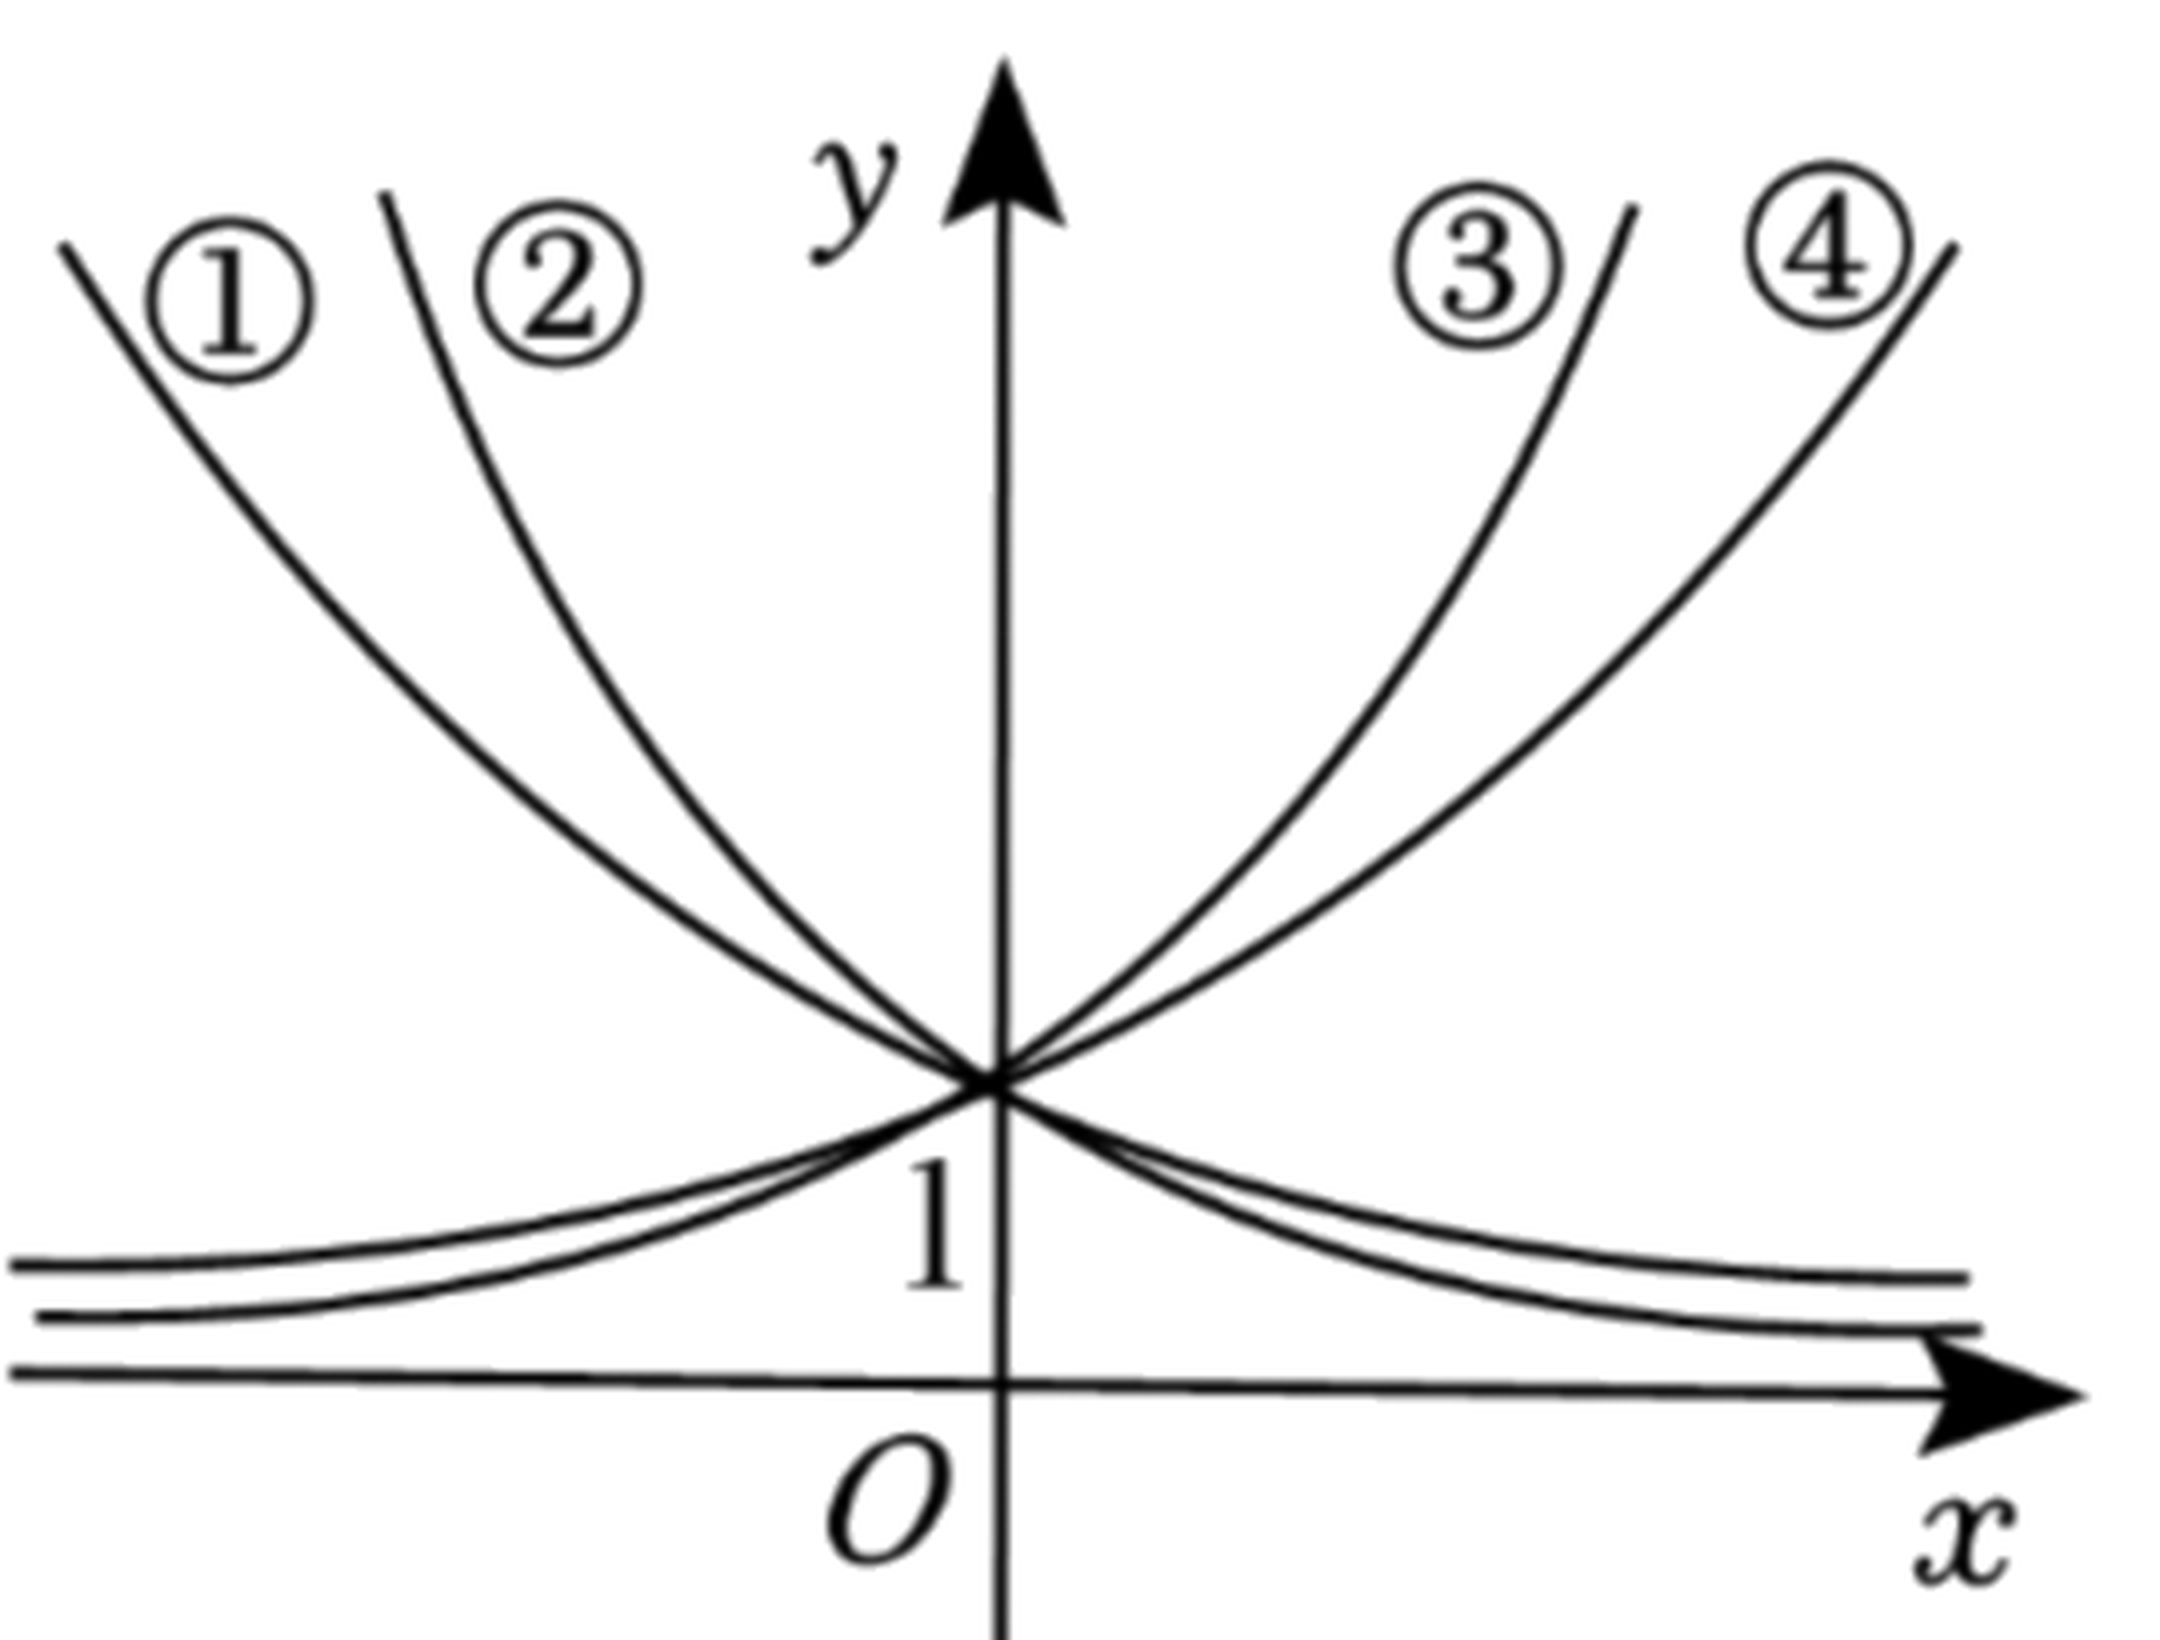
\includegraphics[width=0.40\textwidth]{figures/gao148_q15.png}
\end{center}

\ifanswer
\solbegin
\step{由函数图象得函数① $y=a^x$；② $y=b^x$ 为减函数，且 $x=1$ 时，$b^1<a^1$，}
\step{所以 $0<b<a<1$，}
\step{由函数图象得函数③ $y=c^x$；④ $y=d^x$ 为增函数，且 $x=1$ 时，$c^1>d^1$，}
\step{所以 $c>d>1$，}
\step{所以 $b<a<d<c$. 故选 $B$.}
\solend
\fi

% === Q16 ===：题目配图（关于 y 轴对称的幂函数曲线，三版都出），\needvspace 守卫放 \item 之前；$p$、$q\in\Z$；"图象"照录；解析 2 行
\needvspace{8cm}
\item 已知幂函数 $y=x^{\frac{p}{q}}$（$p$、$q\in\Z$ 且 $p$、$q$ 互质）的图象关于 $y$ 轴对称，如图所示，则\mbox{（\quad）}

\keepwithprev
A. $p$、$q$ 均为奇数，且 $\dfrac{p}{q}>0$\qquad\qquad B. $q$ 为偶数，$p$ 为奇数，且 $\dfrac{p}{q}<0$

C. $q$ 为奇数，$p$ 为偶数，且 $\dfrac{p}{q}>0$\qquad\qquad D. $q$ 为奇数，$p$ 为偶数，且 $\dfrac{p}{q}<0$

\begin{center}
% 关于 y 轴对称的幂函数曲线图取 04 页右下，去粉色水印、去色、4× LANCZOS 放大；三版都出
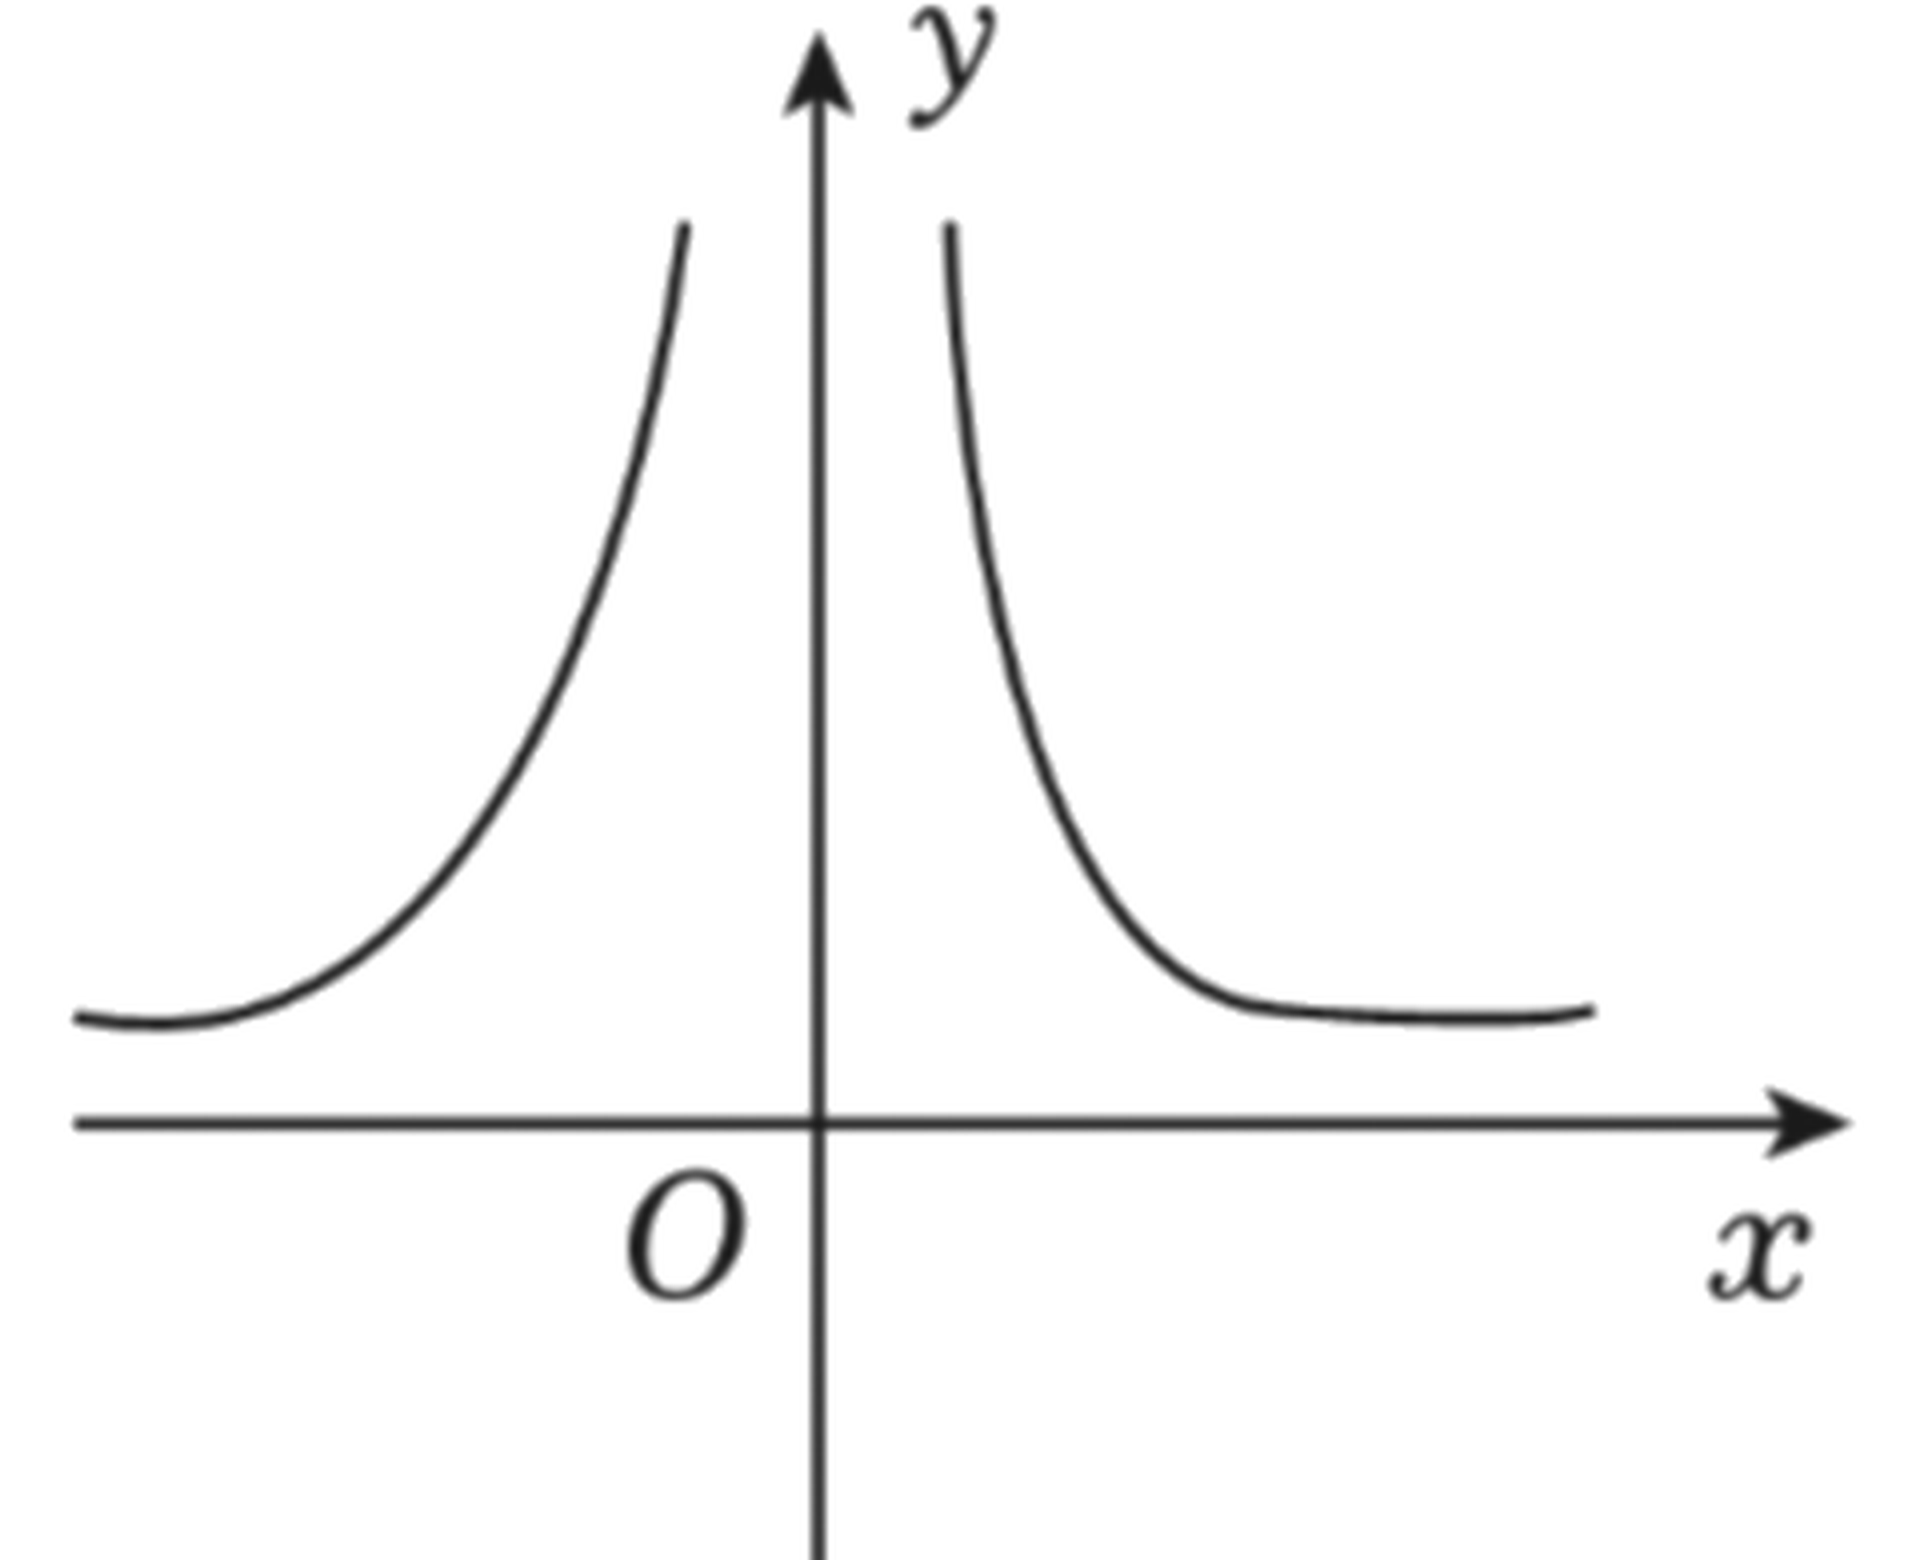
\includegraphics[width=0.36\textwidth]{figures/gao148_q16.png}
\end{center}

\ifanswer
\solbegin
\step{因为函数为偶函数，所以 $p$ 为偶数，且由图象形状判定 $\dfrac{p}{q}<0$.}
\step{又 $p$、$q$ 互质，所以 $q$ 为奇数. 故选 $D$.}
\solend
\fi

\end{enumerate}

\bigsec{三、解答题}

\begin{enumerate}
\setcounter{enumi}{16}

% === Q17 ===：\overline{B}／\varnothing／\R／\mid 逐处照录；解析 8 行
\item 已知集合 $A=\left\{x\mid \dfrac{5}{2x+1}>1\right\}$，$B=\{x\mid x^2+(a+3)x+3a<0,a\in\R\}$.

(1) 求 $A$.

(2) 若全集 $U=\R$，且 $A\cap\overline{B}=\varnothing$，求实数 $a$ 的取值范围.

\ifanswer
\solbegin
\step{(1) $\dfrac{5}{2x+1}>1$，即 $\dfrac{5}{2x+1}-1>0$，即 $\dfrac{4-2x}{2x+1}>0$，即 $(2x+1)(x-2)<0$，}
\step{解得 $-\dfrac{1}{2}<x<2$，所以 $A=\left(-\dfrac{1}{2},2\right)$；}
\step{(2) $x^2+(a+3)x+3a<0$，即 $(x+3)(x+a)<0$，}
\step{全集 $U=\R$，且 $A\cap\overline{B}=\varnothing$，}
\step{当 $a<3$ 时，解得 $-3<x<-a$，则 $\overline{B}=(-\infty,-3)\cup(-a,+\infty)$，}
\step{此时 $-a\geqslant2$，解得 $a\leqslant-2$，}
\step{当 $a\geqslant3$ 时，不满足 $A\cap\overline{B}=\varnothing$，}
\step{故实数 $a$ 的取值范围是 $(-\infty,-2]$.}
\solend
\fi

% === Q18 ===：cases 块整体算一个印刷行；解析 6 行
\item 已知幂函数经过点 $(2,4)$.

(1) 当 $x=\dfrac{1}{2}$ 时，求函数的值；

(2) 是否存在实数 $m$、$n$，使得该函数在区间 $[m,n]$ 上最小值为 $6m-8$，最大值为 $6n-8$？若存在，求出 $m$、$n$ 的值，若不存在，请说明理由.

\ifanswer
\solbegin
\step{(1) 设幂函数的解析式是 $y=x^\alpha$，则 $2^\alpha=4$，解得 $\alpha=2$，}
\step{故 $f(x)=x^2$，$f\left(\dfrac{1}{2}\right)=\dfrac{1}{4}$；}
\step{(2) 因为 $f(x)\geqslant0$，所以 $6m-8\geqslant0$，$m\geqslant\dfrac{4}{3}$，}
\step{由函数 $f(x)$ 在 $(0,+\infty)$ 严格增，得函数 $f(x)$ 在 $(m,n)$ 严格增，}
\step{所以 $\begin{cases}f(m)=6m-8\\f(n)=6n-8\end{cases}$ 且 $m<n$，解得 $m=2$，$n=4$，}
\step{故存在 $m=2$，$n=4$ 满足题意.}
\solend
\fi

% === Q19 ===：7 处评分档照 高一54／64 成例排 \dots\dots N 分；判别式高 \Delta；解析 9 行
\item 已知方程 $x^2+6mx+9m-2=0$，且 $x_1,x_2$ 是方程的两个不同的实数根.

(1) 若 $m=1$，求 $\dfrac{1}{x_1}+\dfrac{1}{x_2}$ 的值；

(2) 若 $m\in\R$，且 $x_1^2+x_2^2<4$，求 $m$ 取值范围.

\ifanswer
\solbegin
\step{(1) 当 $m=1$ 时，方程为 $x^2+6x+7=0$，\dots\dots1 分}
\step{则 $x_1+x_2=-6,x_1\cdot x_2=7$，\dots\dots2 分}
\step{$\dfrac{1}{x_1}+\dfrac{1}{x_2}=\dfrac{x_1+x_2}{x_1\cdot x_2}=-\dfrac{6}{7}$\dots\dots3 分}
\step{(2) $x_1+x_2=-6m,x_1\cdot x_2=9m-2$\dots\dots2 分}
\step{因为 $x_1^2+x_2^2=(x_1+x_2)^2-2x_1\cdot x_2$，所以 $(x_1+x_2)^2-2x_1\cdot x_2<4$，}
\step{所以 $36m^2-2(9m-2)<4$，解得 $0<m<\dfrac{1}{2}$\dots\dots2 分}
\step{又因为方程有两个不同的根，所以 $\Delta=36m^2-4(9m-2)>0$，}% 判别式原卷印等腰偏高粗三角 $\Delta$，照录（放大 07 页 q19_delta3.png／diag_band_q19.png 确认）
\step{解得 $m<\dfrac{1}{3}$ 或 $m>\dfrac{2}{3}$\dots\dots2 分}
\step{所以 $0<m<\dfrac{1}{3}$\dots\dots2 分}
\solend
\fi

% === Q20 ===：题目配图（矩形蔬菜温室，三版都出），\needvspace 守卫放 \item 之前；单位 \mathrm{m}／\mathrm{m}^2；解析 10 行
\needvspace{8cm}
\item 某村计划建造一个室内面积为 $600\mathrm{m}^2$ 的矩形蔬菜温室，在室内，沿左、右两侧与后侧内墙各保留 $2\mathrm{m}$ 宽的通道，沿前侧内墙保留 $4\mathrm{m}$ 宽的空地.

\begin{center}
% 矩形蔬菜温室示意图取 07 页右侧，去粉色水印、去色、4× LANCZOS 放大；三版都出
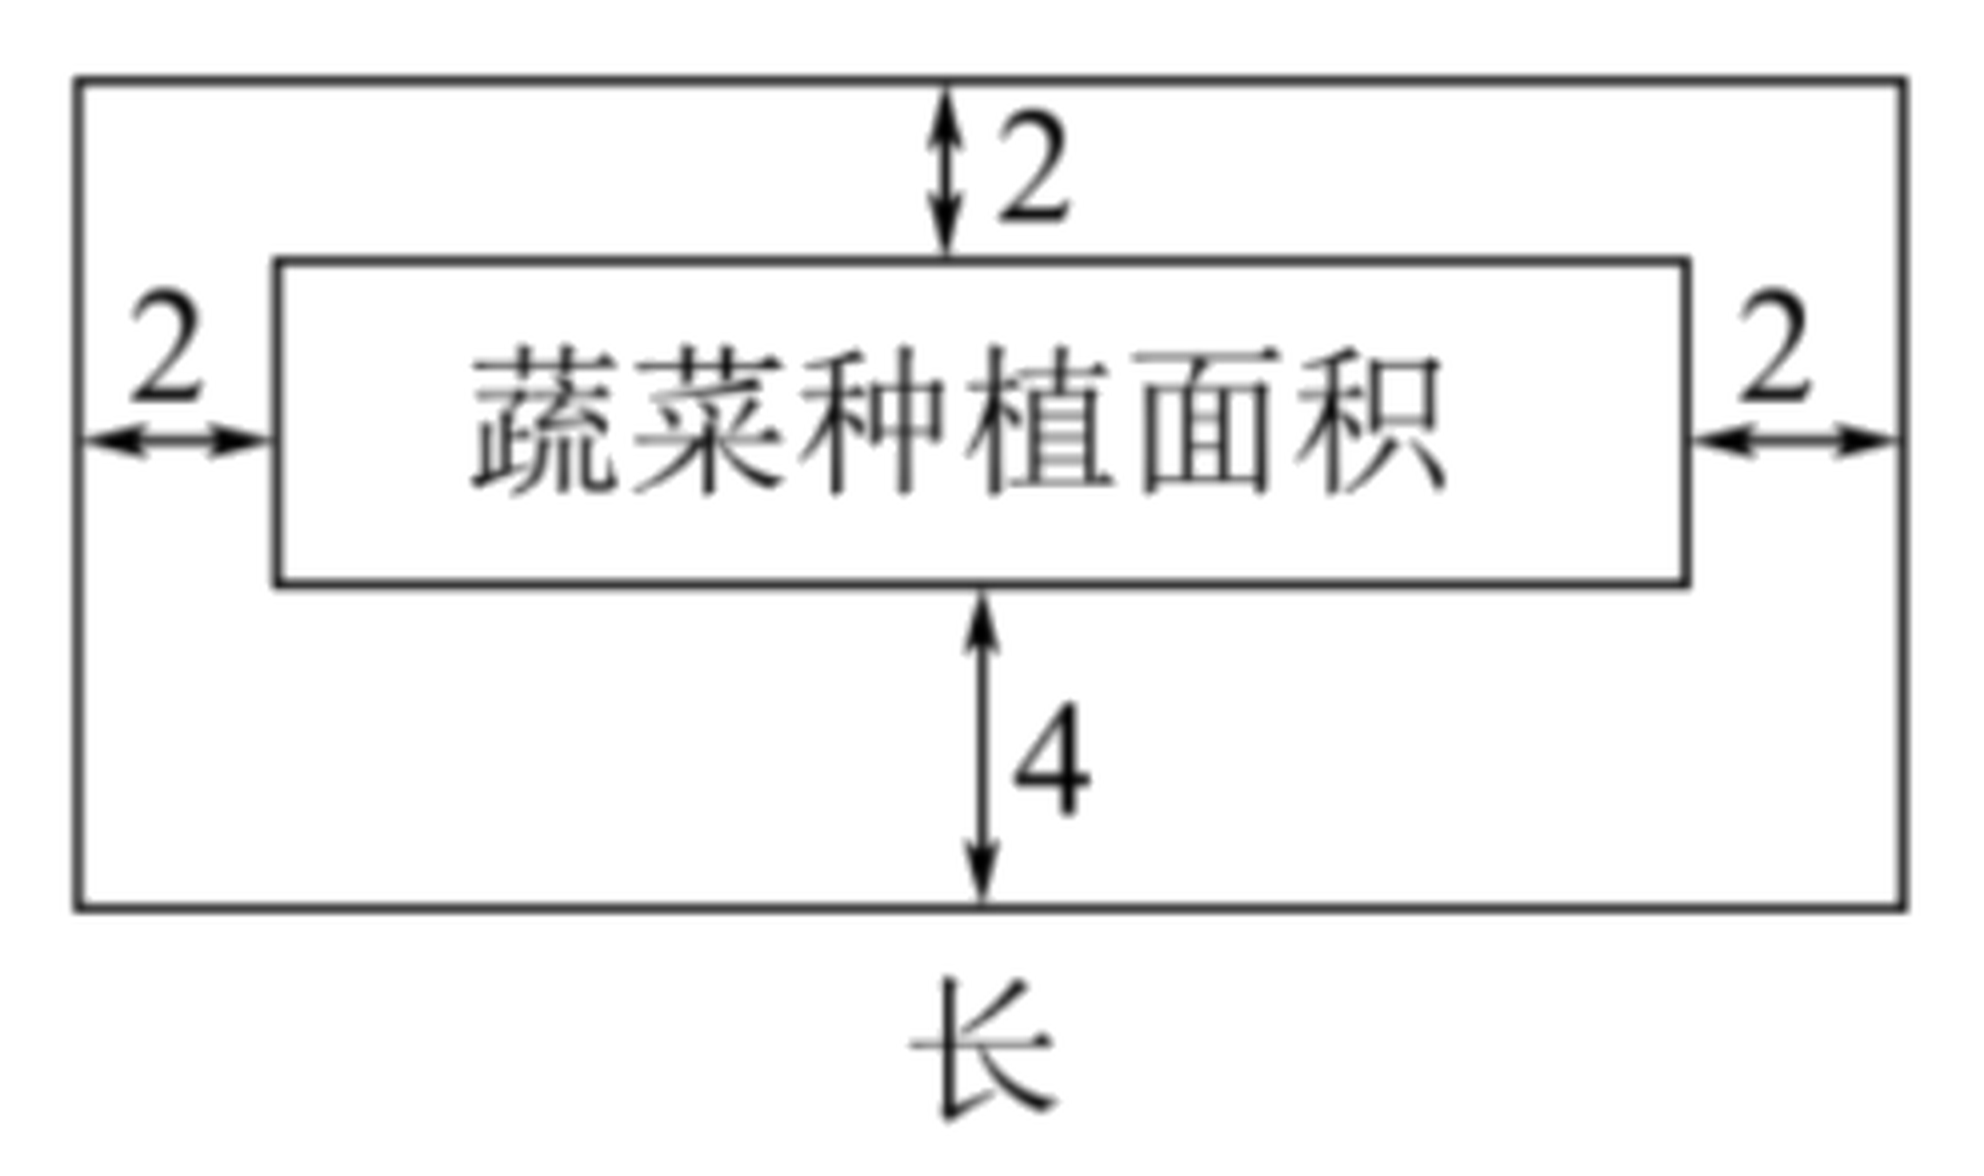
\includegraphics[width=0.45\textwidth]{figures/gao148_q20.png}
\end{center}

(1) 写出蔬菜的种植面积关于矩形温室的长之间的关系式.

(2) 当矩形温室的边长各为多少时，蔬菜的种植面积最大？最大种植面积是多少？

\ifanswer
\solbegin
\step{(1) 设蔬菜的种植面积为 $y\mathrm{m}^2$，矩形温室的长为 $x\mathrm{m}$，}
\step{则矩形温室的宽为 $\dfrac{600}{x}\mathrm{m}$，}
\step{种植蔬菜矩形的长为 $(x-4)\mathrm{m}$，宽为 $\left(\dfrac{600}{x}-6\right)\mathrm{m}$，}
\step{所以 $y=(x-4)\left(\dfrac{600}{x}-6\right)(4<x<100)$；}
\step{(2) 因为 $y=(x-4)\left(\dfrac{600}{x}-6\right)=624-\left(6x+\dfrac{2400}{x}\right)$，}
\step{因为 $6x+\dfrac{2400}{x}\geqslant2\sqrt{6x\cdot\dfrac{2400}{x}}=240$，}
\step{当且仅当 $6x=\dfrac{2400}{x}$，即 $x=20$ 时取等号，}
\step{所以 $y=624-\left(6x+\dfrac{2400}{x}\right)\leqslant624-240=384$.}
\step{即当矩形温室的一边长为 $20\mathrm{m}$，另一边长为 $30\mathrm{m}$ 时，}
\step{蔬菜的种植面积最大，最大为 $384\mathrm{m}^2$.}
\solend
\fi

% === Q21 ===：3 问、cases 块整体算一个印刷行；判别式高 \Delta；解析 19 行（末行续 09 页）
\item 二次函数 $f(x)=ax^2+bx+c$ 满足对任意的 $x\in\R$，$x-1\leqslant f(x)\leqslant x^2-x$ 恒成立.

(1) 求证：$f(1)$ 为定值；

(2) 若 $f(0)=-\dfrac{1}{4}$，求二次函数 $f(x)$ 的表达式；

(3) 求 $a+2b+5c$ 的取值范围.

\ifanswer
\solbegin
\step{(1) 对任意的 $x\in\R$，$x-1\leqslant f(x)\leqslant x^2-x$ 恒成立，则 $0\leqslant f(1)\leqslant0$，}
\step{所以 $f(1)=0$，为定值.}
\step{(2) 由(1)得 $a+b+c=f(1)=0$，由 $f(0)=-\dfrac{1}{4}$，得 $c=-\dfrac{1}{4}$，}
\step{则 $b=\dfrac{1}{4}-a$，$f(x)=ax^2+\left(\dfrac{1}{4}-a\right)x-\dfrac{1}{4}$，}
\step{不等式 $x-1\leqslant f(x)$ 可化为 $ax^2+\left(\dfrac{1}{4}-a\right)x-\dfrac{1}{4}\geqslant x-1$，}
\step{即 $ax^2-\left(a+\dfrac{3}{4}\right)x+\dfrac{3}{4}\geqslant0$，}
\step{一元二次不等式 $ax^2-\left(\dfrac{3}{4}+a\right)x+\dfrac{3}{4}\geqslant0$ 恒成立，则 $\begin{cases}a>0\\\Delta=\left(a+\dfrac{3}{4}\right)^2-3a\leqslant0\end{cases}$，}% 判别式原卷印等腰偏高粗三角 $\Delta$，照录（放大 08 页 q21_delta3.png／diag_band_q21.png 确认）
\step{解得 $a=\dfrac{3}{4}$，}
\step{此时 $f(x)=\dfrac{3}{4}x^2-\dfrac{1}{2}x-\dfrac{1}{4}$，$x^2-x-f(x)=\dfrac{1}{4}(x-1)^2\geqslant0$ 恒成立，}
\step{所以 $f(x)=\dfrac{3}{4}x^2-\dfrac{1}{2}x-\dfrac{1}{4}$.}
\step{(3) 由(1)得 $b=-a-c$，$f(x)=ax^2-(a+c)x+c=(ax-c)(x-1)$，}
\step{不等式 $x-1\leqslant f(x)$ 可化为 $(x-1)(ax-c-1)\geqslant0$，}
\step{一元二次不等式 $(x-1)(ax-c-1)\geqslant0$ 恒成立，则 $a>0$，}
\step{且方程 $(x-1)(ax-c-1)=0$ 有相等的实数根，因此 $c=a-1$，$a>0$，}
\step{不等式 $f(x)\leqslant x^2-x\Leftrightarrow(ax-c)(x-1)\leqslant x^2-x\Leftrightarrow(x-1)[(1-a)x+c]\geqslant0$，}
\step{同理 $1-a>0$，且方程 $(x-1)[(1-a)x+c]=0$ 有相等的实数根，}
\step{因此 $c=a-1$，$a<1$，从而 $c=a-1$，$b=1-2a$，$0<a<1$，}
\step{$a+2b+5c=a+2(1-2a)+5(a-1)=2a-3\in(-3,-1)$，}
\step{所以 $a+2b+5c$ 的取值范围是 $(-3,-1)$.}
\solend
\fi

\end{enumerate}

\end{document}
"
%
% ① 原始材料：微信公众号"魔都数学加油站"文章，连载"27学年高一148"，原文标题
% "27学年高一148——2026-2027年上海市新川中学高一上期中"（2026-11-21 推送）；
% 原文链接：https://mp.weixin.qq.com/s/Alhmwb3sSLQMp_wjzoAVyA 。
% 正文为 9 张 PNG 页（01/03/04/07/08/09 为 2560×3620，02/05/06 为 4762×6735，
% 同一篇各页分辨率混排，逐页按各自分辨率裁图核对，别按预览比例换算裁框）。
% 体例：混合体例讲评版——19 题中 Q4、Q5 只印【答案】、无【解析】；Q13 的答案"C"
% 直接印在题干括号内、无【答案】/【解析】段；其余 16 题印【解析】（逐题核实，见 ② ②）。
% 题目、答案、解析均据原图转录；卷面粉红色水印"魔都数学加油站"及公众号页脚未录入。
% 全卷插图清单（逐页通读 9 页确认）：4 幅题目配图，均三版都出、均非【解析】内配图：
%   · Q12 幂函数曲线族图（03 页右侧：x/y 轴、O、A(1,0)、B(0,1)、M、N 与两族
%     y=x^α／y=x^β 曲线、线段 AB、虚线），题干"（如图）"处，裁 figures/gao148_q12.png；
%   · Q15 四条指数函数曲线图（04 页右侧：①②③④ 四曲线同过 (0,1)、x/y 轴、O、
%     y 轴刻度 1），题干"如图"处，裁 figures/gao148_q15.png；
%   · Q16 关于 y 轴对称的幂函数曲线图（04 页右下：x/y 轴、O、两支上翘曲线），
%     题干"如图所示"处，裁 figures/gao148_q16.png；
%   · Q20 矩形蔬菜温室示意图（07 页右侧：大矩形＋内框"蔬菜种植面积"＋2/2/4
%     通道标注＋"长"），题干处，裁 figures/gao148_q20.png；
%   其余各页逐页确认无其它题目配图、无【解析】内配图、无表格，亦无"题干写如图而
%   源码漏图"一处；Q19 解析行末的虚线"----N 分"为评分档（非图），Q18／Q21 的
%   cases 块为数学块（非图）。4 图均取自原卷截图，去粉色水印、去色、4× LANCZOS 放大。
%
% 卷首标题：原卷印作"2026-2027 年新川中学高一上期中"，年份区间按全稿惯例排 en dash；
% 原卷卷面未印副标题，本稿按同期中卷（高一140／141／143／144／145／146／147）知识模块
% 口径补出"集合与常用逻辑用语、不等式、函数"。
%
% 题号体例（逐页核实定稿）：本卷共 19 题——一、填空题 3—12（10 题）、
% 二、选择题 13—16（4 题）、三、解答题 17—21（5 题）。
% 三节分别 \setcounter{enumi}{2}／{12}／{16}。原卷从第 3 题起、无第 1、2 题，
% 本稿保留原题号；全卷无附加题节、无 Q22（Q21 解析末行"所以 a+2b+5c 的取值范围是
% (-3,-1)."为全卷收尾，09 页下半仅水印、无正文）。
%
% ② 与原卷的排版差异：
%   ① 原文从第 3 题起，本稿保留原题号；共 19 题三节；
%   ② 混合体例逐题核实：Q4（反证法"假设的内容"）、Q5 只印【答案】、无【解析】，
%      按 高一140 第 5 题／高一145 Q3 成例提 \ans{}、不补造解析；Q13 答案"C"直接
%      印在题干括号内（" ( C ) "）、全卷无该题【答案】/【解析】段，按 高一84 Q13／
%      高一37 Q13／高一53 Q13 成例括号 \mbox{（\quad）} 留空、另提 \ans{$C$}；
%      其余 16 题印【解析】、用 \solbegin…\solend，选择题答案在解析末句"故选 X"
%      （Q14 选 D、Q15 选 B、Q16 选 D，逐个放大原图核实）、题干括号留空、不另提
%      \ans{}；答案版【答案】/【解析】标记数 = 19（3 个 \ans ＋ 16 个 \solbegin）
%      = 全卷题数；
%   ③ 原卷卷面未印副标题，本稿按知识模块口径补出；
%   ④ 原卷填空横线按全稿惯例排 \blankline[4.4em]；选择题括号排 \mbox{（\quad）}、
%      选项段前按惯例加 \keepwithprev；Q13／Q16 四选项为两行两列、Q14／Q15 选项
%      为一行，照原卷分行；解答题不留作答区、不加 \anspace（原卷为讲评版，
%      与 129／131／132／133／136／140／141／143／144／145／146 同）；
%   ⑤ 数集：Q11"在 R 上定义运算"、Q13"x、y∈R"、Q16"p、q∈Z"、Q17"a∈R"
%      "U=R"、Q19"m∈R"、Q21"x∈R" 原卷印斜体 R/Z，按全稿惯例统一改 \R／\Z
%      （本卷未出现 N，\N^* 无对应处）；绝对值排 \lvert…\rvert（Q9／Q14），
%      集合描述竖线排 \mid（Q17）；不等号按全稿惯例排 \leqslant／\geqslant；
%      补集照原卷上划线排 \overline{B}（Q17 题干 1 处＋解析 3 处）；空集
%      \varnothing（Q17 题干 1 处＋解析 2 处）；\subset（Q3 题干 {a}⊂M）与
%      \subseteq（Q3 题干 M⊆{a,b,c,d}）逐处照录不统一（放大 01 页 q3_subset.png）；
%   ⑥ 子题标号 (1)(2)(3) 半角括号照录；圈数字 ①—⑥ 在文本模式（Q14 六个结论、
%      Q15 曲线编号与其解析、Q14 解析"对①…对⑥"），按 common.sty 划入 CJK 字符类
%      渲染；cases 块整体算一个印刷行；\left…\right 不得拆到不同 $…$ 组；
%      单位 m／m² 排 \mathrm{m}／\mathrm{m}^2（Q20，原卷印正体 m）；
%   ⑦ 题干／解析中的中文弯引号按原卷照录：Q4" ab 可以被 5 整除，那么 a、b 中
%      至少有一个能被 5 整除 "（开引号后有空格、闭引号后空格接"时"）、
%      Q13" x=0 "" xy=0 "（引号内空格），注释内一律 ASCII 引号；
%   ⑧ 半角逗号在数学组之间是全稿惯例、非笔误（Q3"{a,b,c,d}"、Q6"$x,y$"
%      "$x=\frac13,y=\frac16$"、Q10、Q11"$a=-2,b=-1"、Q12"$\alpha=\log..,\beta=..$"、
%      Q14"$a+b<0,a-b<0$"、Q17、Q19"$x_1+x_2=-6,x_1\cdot x_2=7$"、Q20、Q21 等），
%      逐处照录别改全角；行末西文句点照录为 ASCII `.`；行中全角逗号／顿号照录；
%   ⑨ "图像／图象"逐处放大核：全卷 9 处均印"图象"（象，无亻）、未见"图像"，
%      逐处照录未统一改动（Q8 题干/解析各 1、Q12 题干 2、Q15 题干 1／解析 2、
%      Q16 题干 1／解析 1；放大 02/03/04/05 页 /tmp/gao148/zoom/my_wide_a.png、
%      my_wide_b.png 与宋体参考"象／像"并排确认）；
%   ⑩ 判别式 Δ/△ 混用是照录项：Q11 解析"△=1−4(−a²+a+1)<0"印扁等边空心
%      三角 \triangle；Q19 解析"Δ=36m²−4(9m−2)>0"、Q21 解析 cases 块
%      "Δ=(a+3/4)²−3a≤0" 两处印等腰偏高粗三角 \Delta，逐处放大判断、照录
%      不统一（参照 高一142／144／145 头注④口径，详见 ④）；
%   ⑪ 一条 \step = 原卷解析的一个印刷行，cases 块整体算一个印刷行；别把原卷折行
%      并起来、别把一行拆多条。Q3 六行、Q7 五行（01 页末首行＋02 页顶四行）、
%      Q9 七行、Q11 五行、Q14 八行（对② 的两行公式各占一印刷行）、Q17 八行、
%      Q18 六行、Q19 九行（7 处评分档附在行末）、Q20 十行、Q21 十九行
%      均按印刷行逐条断，不丢行；
%   ⑫ 配图：4 幅均为题目配图（三版都出），放 \item 内题干之后 \begin{center}；
%      大图块加 \needvspace 守卫把整块推走（守卫放 \item 之前，见 高一145 Q14/Q20
%      成例与切页审计 B 类坑）；三版切页审计均"合计异常：无"；
%   ⑬ 跨页续印按题合并：Q3/4/5 在 01 页；Q6 题干＋解析在 01 页；Q7 题干在 01 页
%      末、解析首行在 01 页末续 02 页顶四行；Q8/9/10 在 02 页（Q9 解析续 02 页下半、
%      Q10 题干与解析前 2 行在 02 页末）；Q10 解析末行续 03 页顶；Q11/12 在 03 页、
%      "二、选择题"标题与 Q13/14 题干在 03 页下半；Q13 无解析；Q14 解析在 04 页顶、
%      Q15 题干＋图＋选项＋解析在 04 页、Q16 题干＋图在 04 页末；Q16 选项＋解析＋
%      "三、解答题"标题＋Q17 题干＋解析在 05 页、Q18 题干首句在 05 页末；Q18 题干
%      续＋解析、Q19 题干＋解析前 5 行在 06 页；Q19 解析续 4 行＋Q20 题干＋图＋
%      解析（10 行全部）在 07 页，末行"蔬菜的种植面积最大，最大为 384m²."收尾；
%      Q21 题干＋解析前 18 行在 08 页；Q21 解析末行"所以 a+2b+5c 的取值范围是
%      (-3,-1)."在 09 页上半（09 页下半仅水印、无正文）。本稿按题连排，不丢行、
%      不并折行；
%   ⑭ 原卷解析内无红色"法一／法二"之类小标题，故本卷无 \stepm；水印
%      "魔都数学加油站"红色不录入；Q19 解析 7 处评分档（1/2/3/2/2/2/2 分）
%      原卷在行末印一串虚线，本稿照 高一54／64 成例排 \dots\dots N 分，
%      分值逐处照录、位置不变。
%
% ③ 行数复核：一条 \step／\stepm = 原卷解析的一个印刷行，cases 块作一个印刷行计。
%   逐题数（主会话逐页核对定稿）：Q3：6；Q4：0（只印【答案】、提 \ans{}）；
%   Q5：0（只印【答案】、提 \ans{}）；Q6：2；Q7：5；Q8：2；Q9：7；Q10：3；
%   Q11：5；Q12：2；Q13：0（答案印在题干括号内、另提 \ans{}）；Q14：8；Q15：5；
%   Q16：2；Q17：8；Q18：6；Q19：9；Q20：10；Q21：19。
%   合计 99 条 \step（本卷无 \stepm：解析内无红色"法一／法二"类小标题），
%   与原卷逐题印刷行相等。全卷 16 题设 \solbegin…\solend ＋ 3 处 \ans{}，
%   答案版【答案】/【解析】标记数 = 19 = 全卷题数。
%
% ④ 判别式／子集符号结论（逐处放大原图照录、不得统一，主会话像素级复核）：
%   判别式全卷 3 处，两形混用逐处照录不统一（参照 高一142／144／145 头注④口径）：
%     · Q11 解析"△=1−4(−a²+a+1)<0" 原卷印扁等边空心三角（宽>高、细线），
%       照录 \triangle（放大 03 页 /tmp/gao148/zoom/q11_delta3.png、
%       delta_montage.png 确认）；
%     · Q19 解析"Δ=36m²−4(9m−2)>0" 原卷印等腰偏高粗三角（高>宽），
%       照录 \Delta（放大 07 页 /tmp/gao148/zoom/q19_delta3.png 确认）；
%     · Q21 解析 cases 块"Δ=(a+3/4)²−3a≤0" 原卷印等腰偏高粗三角（高>宽），
%       照录 \Delta（放大 08 页 /tmp/gao148/zoom/q21_delta3.png 确认）。
%   子集／补集：Q3 题干"{a}⊂M⊆{a,b,c,d}" 前者印单线 ⊂、无下划线，照录 \subset；
%     后者印带下划线 ⊆，照录 \subseteq（放大 01 页 /tmp/gao148/zoom/q3_subset.png
%     确认）；Q17 题干 1 处＋解析 3 处共 4 处 \overline{B} 照原卷上划线
%     （B 上横线、非 C_U B）；空集 \varnothing 3 处（Q17 题干 1 处、解析 2 处）；
%     Q17 集合描述竖线 \mid；数集 \R／\Z 归一见 ② ⑤。
%
% ⑤ 存疑照录（放大原图确认，照录未改、正文对应处另有 % 注）：
%   1. Q3 解析末行"所以 M 一共有 3+3+1+1=8 个" 原卷印 $3+3+1+1=8$，按上文
%      四行应为 $1+3+3+1=8$（疑为原卷加数顺序笔误，和仍为 8），放大 01 页
%      /tmp/gao148/zoom/my_q3_sol.png 确认，照录未改。
%   2. Q13 答案"C"直接印在题干括号内、全卷无该题【答案】/【解析】段，按
%      高一84 Q13 成例括号留空、另提 \ans{$C$}（见 ② ②），未补造解析。
%   3. Q19 解析 7 处评分档（"----N 分"）原卷印一串虚线，本稿照 高一54／64
%      成例排 \dots\dots N 分，分值逐处照录、位置不变。
%   4. 判别式 Q11 扁 \triangle 与 Q19／Q21 高 \Delta 两形混用，逐处照录不统一（见 ④）。
%   5. "图像／图象"全卷 9 处均印"图象"、未见"图像"（见 ② ⑨），逐处放大核实照录，
%      未统一改动。
%   全卷除此 5 类外未发现其它笔误／自相矛盾处。
%
% ⑥ 跨页续印按题合并说明：见 ② ⑬。
%
\documentclass[a4paper,11pt]{article}
\usepackage{common}

\begin{document}

\examtitlest[3]{2026--2027 年新川中学高一上期中}{集合与常用逻辑用语、不等式、函数}

\bigsec{一、填空题}

\begin{enumerate}
\setcounter{enumi}{2}

% === Q3 ===：题干 {a}⊂M⊆{a,b,c,d} 两个子集符号逐处照录；解析 6 行
\item 满足 $\{a\}\subset M\subseteq\{a,b,c,d\}$ 的集合 $M$ 有\blankline[4.4em]个.

\ifanswer
\solbegin
\step{$M$ 是 $\{a,b,c,d\}$ 的子集，但必含有元素 $a$，}
\step{当 $M$ 中只一个元素时，$M=\{a\}$ 只有 1 个；}
\step{当 $M$ 中有二个元素时，$M$ 有 3 个；}
\step{当 $M$ 中有三个元素时，$M$ 有 3 个；}
\step{当 $M$ 中有四个元素时，$M$ 有 1 个；}
\step{所以 $M$ 一共有 $3+3+1+1=8$ 个.}% 原卷印 $3+3+1+1=8$（按上文四行应为 $1+3+3+1$），疑为加数顺序笔误，照录未改（放大 01 页 my_q3_sol.png）
\solend
\fi

% === Q4 ===：原卷只印【答案】、无【解析】，按 高一140 第 5 题成例提 \ans{}；弯引号与空格照录
\item 用反证法证明命题 “ $ab$ 可以被 5 整除，那么 $a$、$b$ 中至少有一个能被 5 整除” 时假设的内容应该是\blankline[4.4em].

\ifanswer
\ans{$a$、$b$ 都不能被 5 整除}
\fi

% === Q5 ===：原卷只印【答案】 $[-2,1)$、无【解析】，提 \ans{}
\item 不等式 $\dfrac{x+2}{x-1}\leqslant0$ 的解集为\blankline[4.4em].

\ifanswer
\ans{$[-2,1)$}
\fi

% === Q6 ===：解析 2 行；半角逗号在数学组之间照录
\item 设 $x,y\in(0,+\infty)$，且 $x+4y=1$，则 $\dfrac{1}{x}+\dfrac{1}{y}$ 的最小值为\blankline[4.4em].

\ifanswer
\solbegin
\step{因为 $\dfrac{1}{x}+\dfrac{1}{y}=(x+4y)\left(\dfrac{1}{x}+\dfrac{1}{y}\right)=5+\dfrac{4y}{x}+\dfrac{x}{y}\geqslant5+2\sqrt{\dfrac{4y}{x}\cdot\dfrac{x}{y}}=9$，}
\step{当且仅当 $\dfrac{4y}{x}=\dfrac{x}{y}$，即 $x=2y$，即 $x=\dfrac{1}{3},y=\dfrac{1}{6}$ 时取等号，故最小值为 9.}
\solend
\fi

% === Q7 ===：题干在 01 页末、解析首行在 01 页末续 02 页顶四行；解析 5 行
\item 若不等式 $x^2+ax+b<0$ 的解集为 $(-3,-1)$，则不等式 $bx^2+ax+1\leqslant0$ 的解集为\blankline[4.4em].

\ifanswer
\solbegin
\step{不等式 $x^2+ax+b<0$ 的解集为 $(-3,-1)$，}
\step{所以方程 $x^2+ax+b=0$ 的两个实数根为 $-3$ 和 $-1$，}
\step{由根与系数的关系得 $a=4$，$b=3$，}
\step{故 $bx^2+ax+1\leqslant0$ 可化为 $3x^2+4x+1\leqslant0$，解得 $-1\leqslant x\leqslant-\dfrac{1}{3}$，}
\step{所求不等式 $bx^2+ax+1\leqslant0$ 的解集为 $\left[-1,-\dfrac{1}{3}\right]$.}
\solend
\fi

% === Q8 ===："图象"照录；解析 2 行
\item 函数 $y=a^{x-2}+2(a>0,a\ne1)$ 的图象必经过定点\blankline[4.4em].

\ifanswer
\solbegin
\step{令 $x-2=0$，得 $x=2$，则 $y=a^0+2=3$，}
\step{所以函数 $y=a^{x-2}+2$ 的图象过定点 $(2,3)$.}
\solend
\fi

% === Q9 ===：解析 7 行；首句末西文句点照录
\item 不等式 $\lvert x+3\rvert+\lvert a-x\rvert>6$ 对一切实数 $x$ 恒成立，则实数 $a$ 的取值范围为\blankline[4.4em].

\ifanswer
\solbegin
\step{$\lvert x+3\rvert$ 表示 $x$ 到 $-3$ 的距离，$\lvert a-x\rvert$ 表示 $x$ 到 $a$ 的距离.}
\step{所以它们的和为 $x$ 到 $-3$ 和 $x$ 到 $a$ 的距离之和，}
\step{当 $x$ 位于 $-3$ 和 $a$ 之间时，距离和取得最小值，}
\step{即两点之间的距离 $\lvert a-(-3)\rvert=\lvert a+3\rvert$，}
\step{若最小值 $\lvert a+3\rvert>6$，则原式对所有 $x$ 恒成立.}
\step{解得 $a+3>6$ 或 $a+3<-6$，即 $a>3$ 或 $a<-9$，}
\step{故 $a\in(3,+\infty)$ 或 $a\in(-\infty,-9)$.}
\solend
\fi

% === Q10 ===：题干与解析前 2 行在 02 页末、解析末行续 03 页顶；解析 3 行
\item 已知 $2^a=3$，$\log_3 5=b$，则 $\log_{15}20=$\blankline[4.4em]（用 $a$、$b$ 表示）.

\ifanswer
\solbegin
\step{因为 $2^a=3$，所以 $a=\log_2 3=\dfrac{\lg3}{\lg2}$，又 $\log_3 5=b=\dfrac{\lg5}{\lg3}$，}
\step{所以 $\lg3=a\lg2$，$\lg5=b\lg3=ba\lg2$，}
\step{则 $\log_{15}20=\dfrac{2\lg2+\lg5}{\lg3+\lg5}=\dfrac{2\lg2+ab\lg2}{a\lg2+ab\lg2}=\dfrac{2+ab}{a+ab}$.}
\solend
\fi

% === Q11 ===：在 \R 上定义运算 \otimes；判别式扁 \triangle 照录；解析 5 行
\item 在 $\R$ 上定义运算 $\otimes:x\otimes y=x(1-y)$，若不等式 $(x-a)\otimes(x+a)<1$ 对任意实数 $x$ 恒成立，则 $a$ 的取值范围是\blankline[4.4em].

\ifanswer
\solbegin
\step{由题意得不等式 $(x-a)\otimes(x+a)<1$ 对任意实数 $x$ 恒成立，}
\step{即不等式 $(x-a)(1-x-a)<1$ 对任意实数 $x$ 恒成立，}
\step{即 $x^2-x-a^2+a+1>0$ 对任意实数 $x$ 恒成立，}
\step{所以 $\triangle=1-4(-a^2+a+1)<0$，解得 $-\dfrac{1}{2}<a<\dfrac{3}{2}$，}% 判别式原卷印扁等边空心三角 $\triangle$，照录（放大 03 页 q11_delta3.png 确认）
\step{所以实数 $a$ 的取值范围为 $\left(-\dfrac{1}{2},\dfrac{3}{2}\right)$.}
\solend
\fi

% === Q12 ===：题目配图（幂函数曲线族，三版都出）；"图象"照录；解析 2 行
\needvspace{8cm}
\item 幂函数 $y=x^\alpha$，当 $\alpha$ 取不同的正数时，在区间 $[0,1]$ 上它们的图象是一族美丽的曲线（如图）. 设点 $A(1,0)$，$B(0,1)$，连接 $AB$，线段 $AB$ 恰好被其中的两个幂函数 $y=x^\alpha$，$y=x^\beta$ 的图象三等分，即有 $BM=MN=NA$，那么 $\alpha\beta=$\blankline[4.4em].

\begin{center}
% 幂函数曲线族图取 03 页右侧，去粉色水印、去色、4× LANCZOS 放大；三版都出
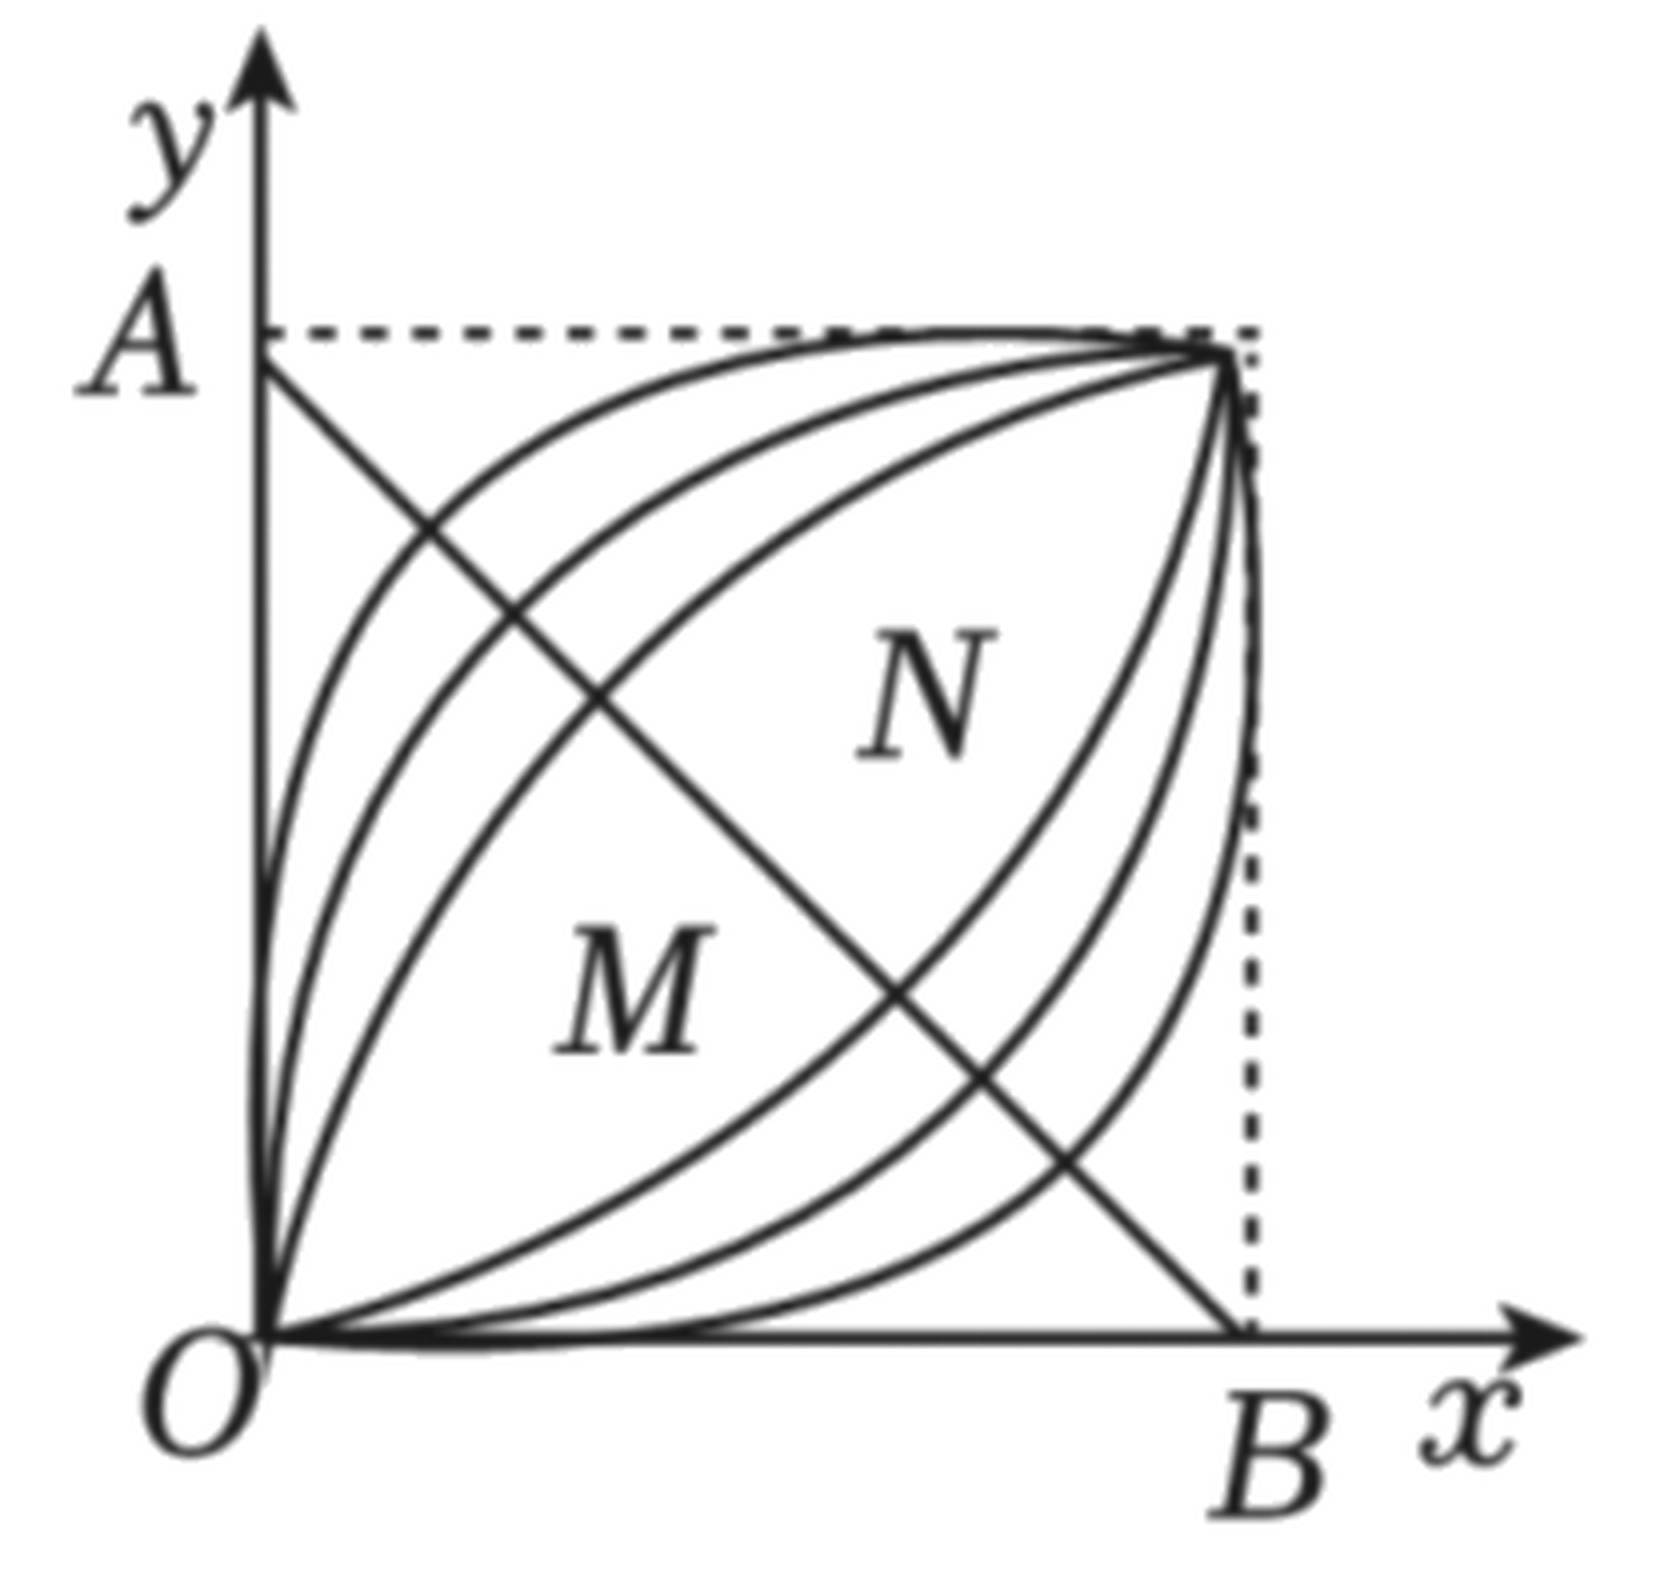
\includegraphics[width=0.40\textwidth]{figures/gao148_q12.png}
\end{center}

\ifanswer
\solbegin
\step{$BM=MN=NA$，点 $A(1,0)$，$B(0,1)$，所以 $M\left(\dfrac{1}{3},\dfrac{2}{3}\right)$，$N\left(\dfrac{2}{3},\dfrac{1}{3}\right)$，}
\step{分别代入 $y=x^\alpha$，$y=x^\beta$，$\alpha=\log_{\frac{2}{3}}\dfrac{1}{3},\beta=\log_{\frac{1}{3}}\dfrac{2}{3}$，$\alpha\beta=\log_{\frac{1}{3}}\dfrac{2}{3}\cdot\log_{\frac{2}{3}}\dfrac{1}{3}=1$.}
\solend
\fi

\end{enumerate}

\bigsec{二、选择题}

\begin{enumerate}
\setcounter{enumi}{12}

% === Q13 ===：答案"C"直接印在题干括号内、全卷无该题【答案】/【解析】段，按 高一84 Q13 成例括号留空、另提 \ans{$C$}；弯引号含空格
\item 若 $x$、$y\in\R$，则 “ $x=0$ ” 是 “ $xy=0$ ” 的\mbox{（\quad）}

\keepwithprev
A. 充要条件\qquad\qquad B. 必要不充分条件

C. 充分不必要条件\qquad\qquad D. 既不充分也不必要条件

\ifanswer
\ans{$C$}
\fi

% === Q14 ===：六个结论（圈数字在文本模式）、四选项一行；解析 8 行（对② 的两行公式各占一印刷行）
\item 若 $a<b<0$，下面有六个结论：① $a^2>b^2$；② $a^3<b^3$；③ $\dfrac{1}{a}<\dfrac{1}{b}$；④ $\dfrac{a}{b}>1$；⑤ $\dfrac{1}{a-b}>\dfrac{1}{a}$；⑥ $\lvert a\rvert>-b$. 其中正确的个数是\mbox{（\quad）}

\keepwithprev
A. 1\qquad\qquad B. 2\qquad\qquad C. 3\qquad\qquad D. 4

\ifanswer
\solbegin
\step{对①：$a^2-b^2=(a+b)(a-b),a+b<0,a-b<0$，故 $a^2-b^2>0$，正确；}
\step{对②：$a^3-b^3=(a-b)(a^2+ab+b^2)=(a-b)\left[\left(a+\dfrac{1}{2}b\right)^2+\dfrac{3}{4}b^2\right],a-b<0$，}
\step{$\left(a+\dfrac{1}{2}b\right)^2+\dfrac{3}{4}b^2>0$，故 $a^3-b^3<0$，正确；}
\step{对③：取 $a=-2,b=-1$，则 $\dfrac{1}{a}=-\dfrac{1}{2},\dfrac{1}{b}=-1,\dfrac{1}{a}>\dfrac{1}{b}$，错误；}
\step{对④：$\dfrac{a}{b}-1=\dfrac{a-b}{b},a-b<0,b<0$，故 $\dfrac{a}{b}-1>0$，正确；}
\step{对⑤：取 $a=-2,b=-1$，则 $\dfrac{1}{a-b}=-1,\dfrac{1}{a}=-\dfrac{1}{2},\dfrac{1}{a-b}<\dfrac{1}{a}$，错误；}
\step{对⑥：要证 $\lvert a\rvert>-b$，即 $-a>-b$，即 $a<b$，正确；}
\step{故选 $D$.}
\solend
\fi

% === Q15 ===：题目配图（四条指数函数曲线，三版都出），\needvspace 守卫放 \item 之前；"图象"照录；解析 5 行
\needvspace{8cm}
\item 如图，曲线①②③④分别是指数函数 $y=a^x$，$y=b^x$，$y=c^x$，$y=d^x$ 的图象，则实数 $a$、$b$、$c$、$d$ 的大小关系为\mbox{（\quad）}

\keepwithprev
A. $a<b<c<d$\qquad B. $b<a<d<c$\qquad C. $d<c<b<a$\qquad D. $c<d<a<b$

\begin{center}
% 四条指数函数曲线图取 04 页右侧，去粉色水印、去色、4× LANCZOS 放大；三版都出
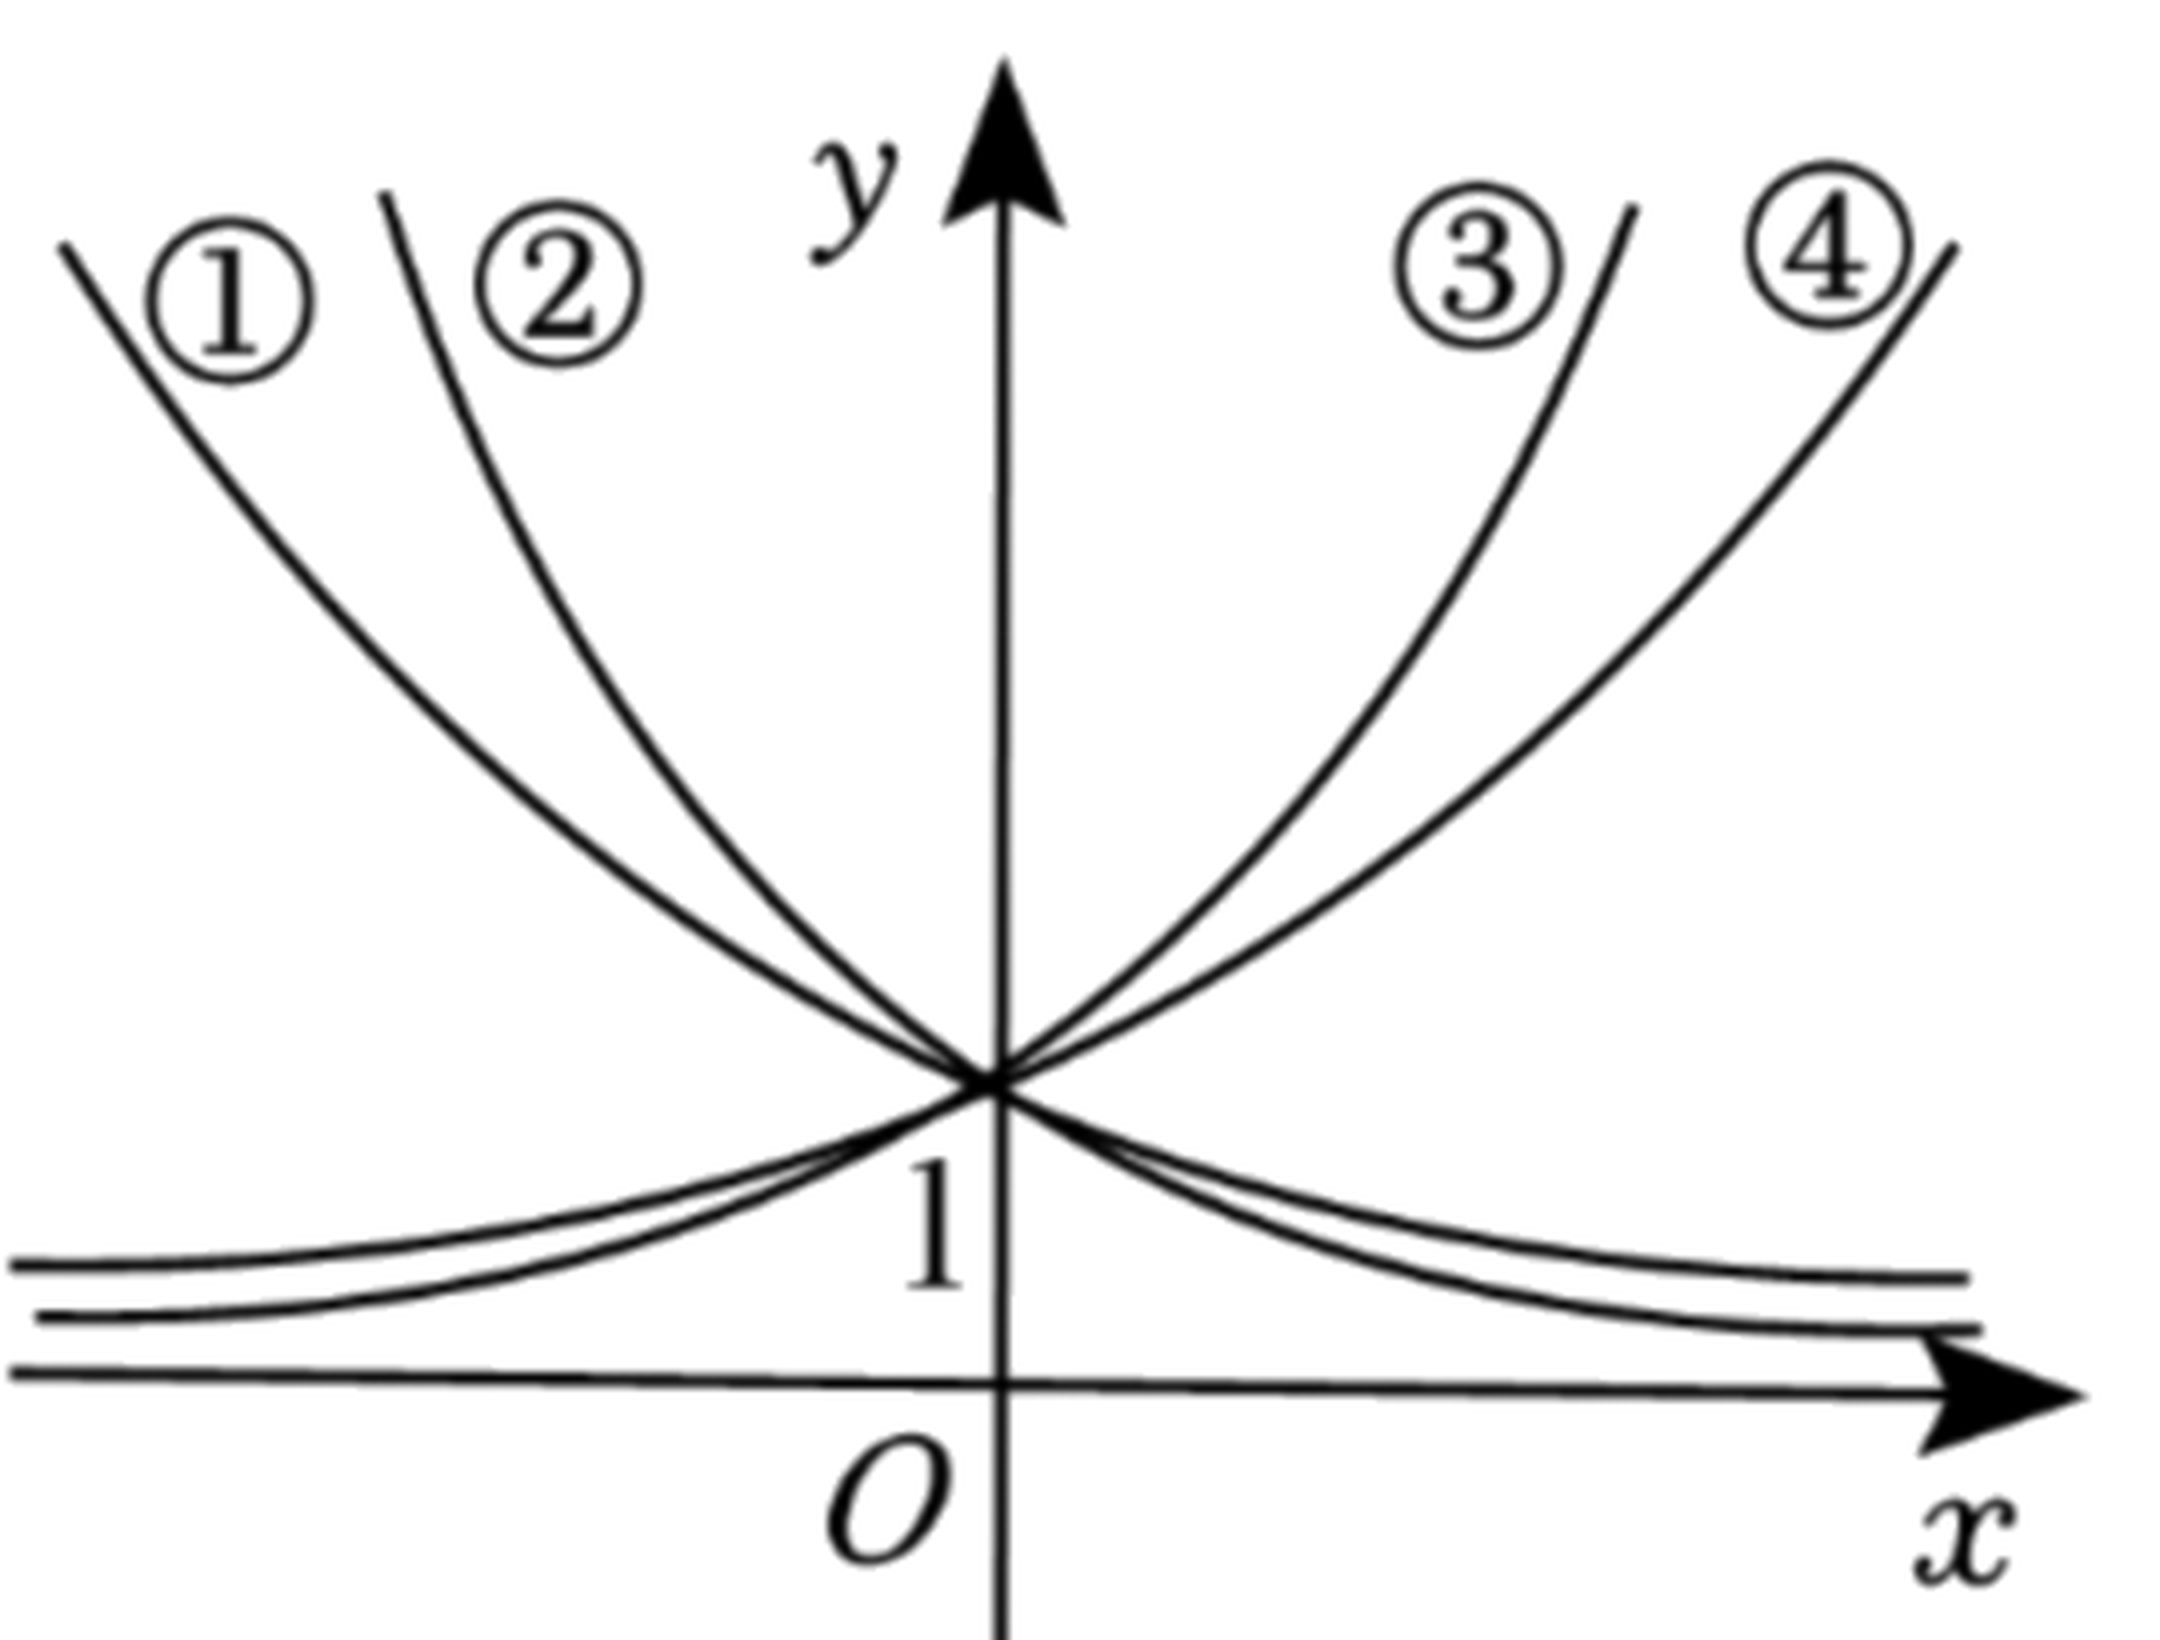
\includegraphics[width=0.40\textwidth]{figures/gao148_q15.png}
\end{center}

\ifanswer
\solbegin
\step{由函数图象得函数① $y=a^x$；② $y=b^x$ 为减函数，且 $x=1$ 时，$b^1<a^1$，}
\step{所以 $0<b<a<1$，}
\step{由函数图象得函数③ $y=c^x$；④ $y=d^x$ 为增函数，且 $x=1$ 时，$c^1>d^1$，}
\step{所以 $c>d>1$，}
\step{所以 $b<a<d<c$. 故选 $B$.}
\solend
\fi

% === Q16 ===：题目配图（关于 y 轴对称的幂函数曲线，三版都出），\needvspace 守卫放 \item 之前；$p$、$q\in\Z$；"图象"照录；解析 2 行
\needvspace{8cm}
\item 已知幂函数 $y=x^{\frac{p}{q}}$（$p$、$q\in\Z$ 且 $p$、$q$ 互质）的图象关于 $y$ 轴对称，如图所示，则\mbox{（\quad）}

\keepwithprev
A. $p$、$q$ 均为奇数，且 $\dfrac{p}{q}>0$\qquad\qquad B. $q$ 为偶数，$p$ 为奇数，且 $\dfrac{p}{q}<0$

C. $q$ 为奇数，$p$ 为偶数，且 $\dfrac{p}{q}>0$\qquad\qquad D. $q$ 为奇数，$p$ 为偶数，且 $\dfrac{p}{q}<0$

\begin{center}
% 关于 y 轴对称的幂函数曲线图取 04 页右下，去粉色水印、去色、4× LANCZOS 放大；三版都出
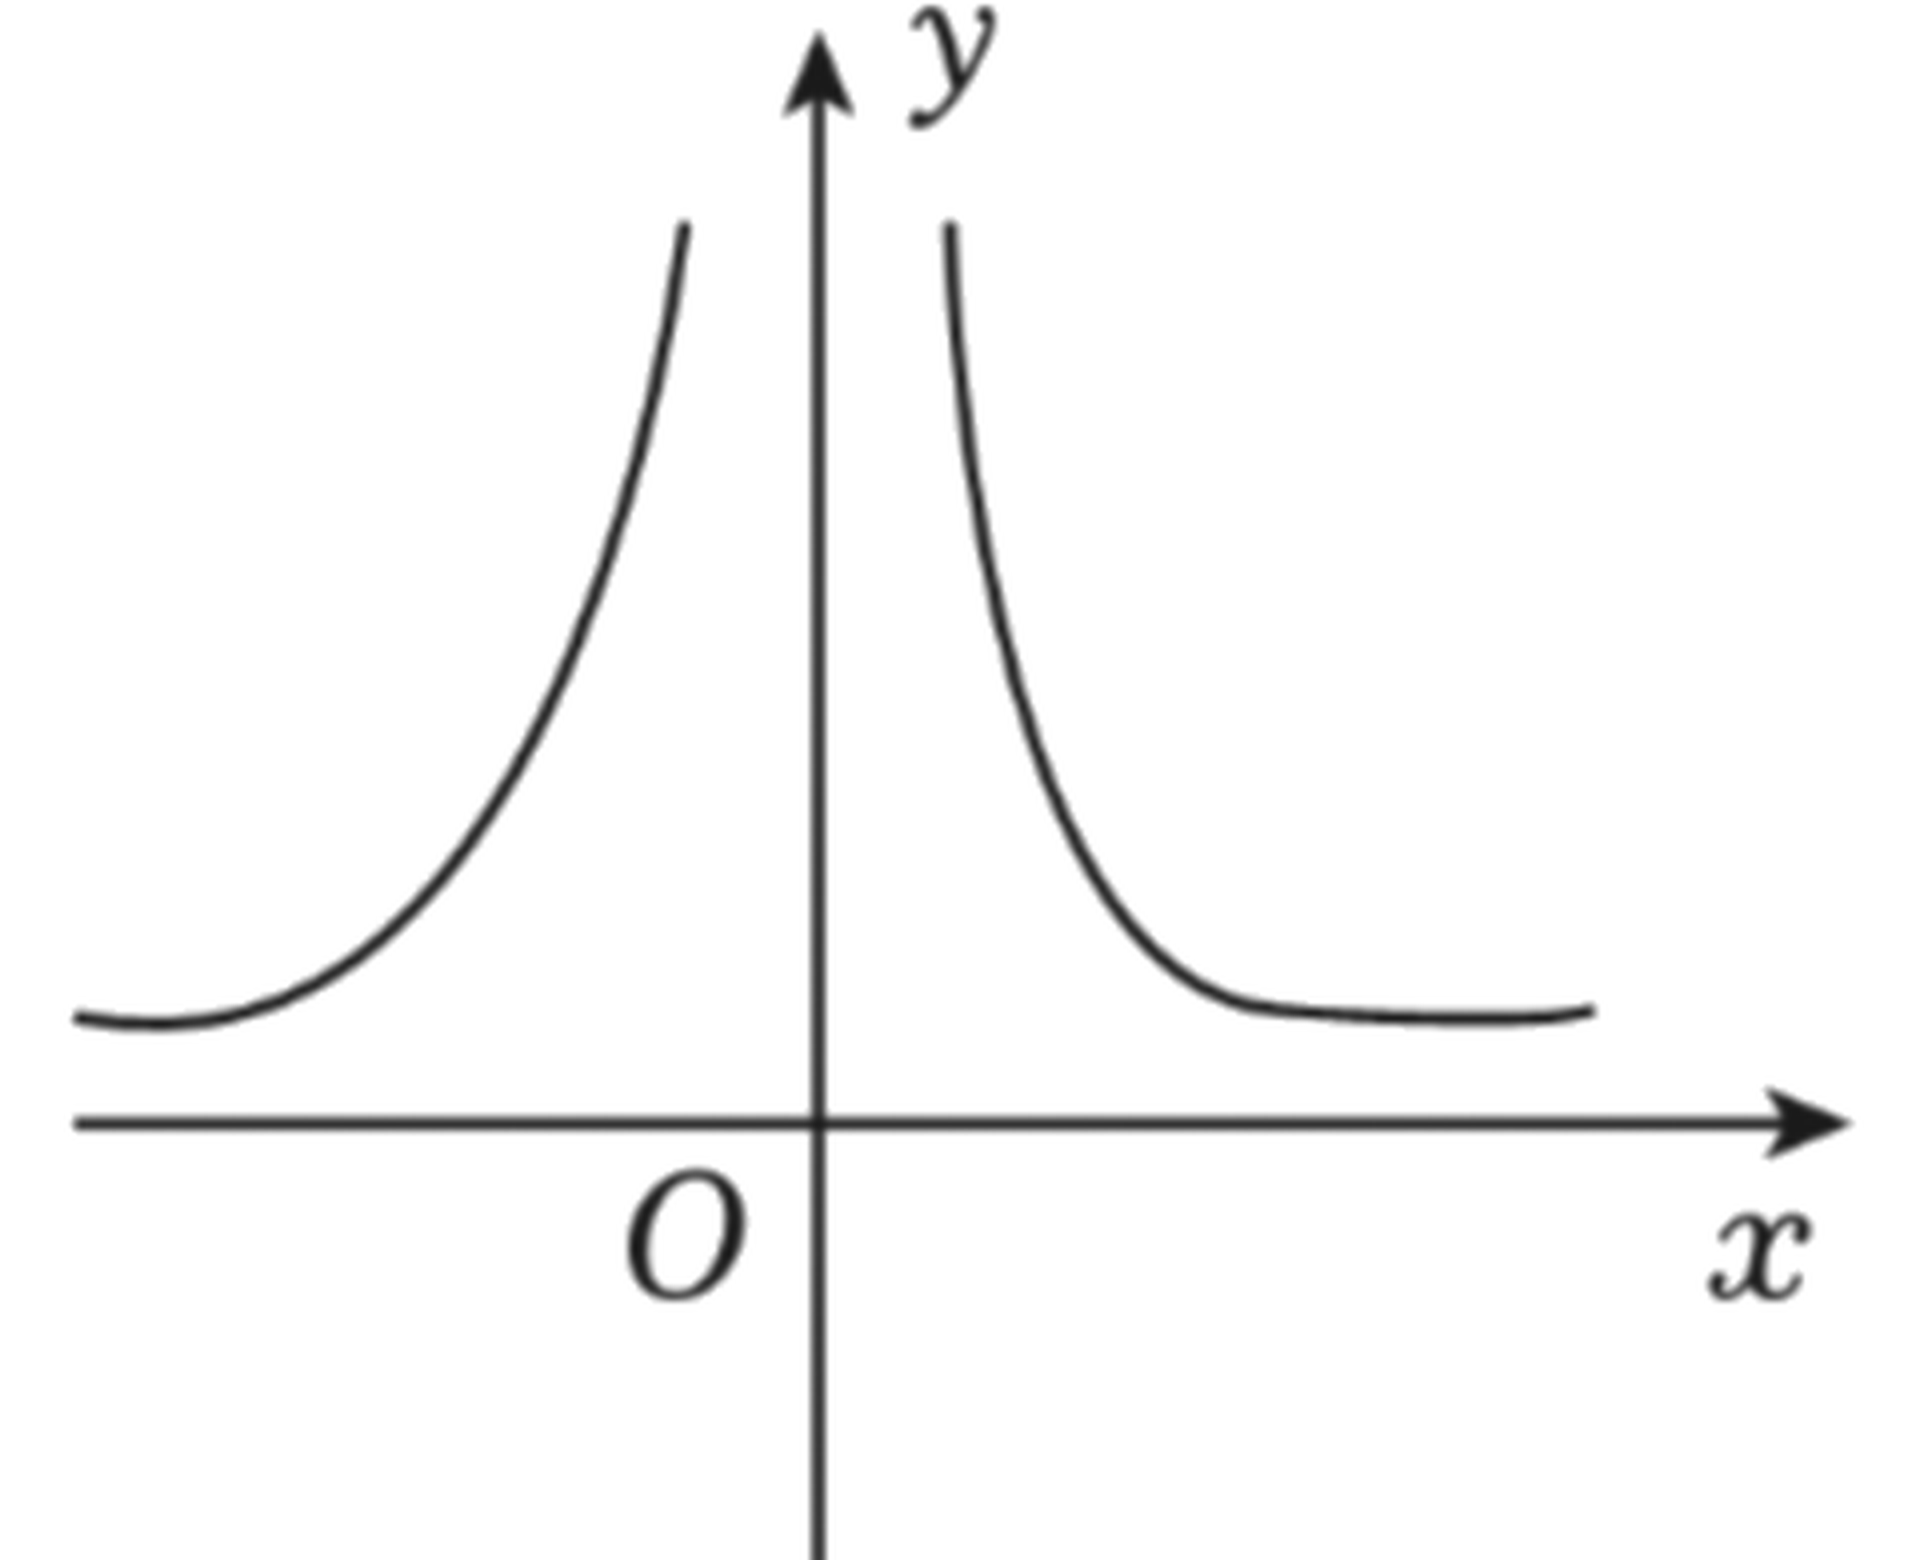
\includegraphics[width=0.36\textwidth]{figures/gao148_q16.png}
\end{center}

\ifanswer
\solbegin
\step{因为函数为偶函数，所以 $p$ 为偶数，且由图象形状判定 $\dfrac{p}{q}<0$.}
\step{又 $p$、$q$ 互质，所以 $q$ 为奇数. 故选 $D$.}
\solend
\fi

\end{enumerate}

\bigsec{三、解答题}

\begin{enumerate}
\setcounter{enumi}{16}

% === Q17 ===：\overline{B}／\varnothing／\R／\mid 逐处照录；解析 8 行
\item 已知集合 $A=\left\{x\mid \dfrac{5}{2x+1}>1\right\}$，$B=\{x\mid x^2+(a+3)x+3a<0,a\in\R\}$.

(1) 求 $A$.

(2) 若全集 $U=\R$，且 $A\cap\overline{B}=\varnothing$，求实数 $a$ 的取值范围.

\ifanswer
\solbegin
\step{(1) $\dfrac{5}{2x+1}>1$，即 $\dfrac{5}{2x+1}-1>0$，即 $\dfrac{4-2x}{2x+1}>0$，即 $(2x+1)(x-2)<0$，}
\step{解得 $-\dfrac{1}{2}<x<2$，所以 $A=\left(-\dfrac{1}{2},2\right)$；}
\step{(2) $x^2+(a+3)x+3a<0$，即 $(x+3)(x+a)<0$，}
\step{全集 $U=\R$，且 $A\cap\overline{B}=\varnothing$，}
\step{当 $a<3$ 时，解得 $-3<x<-a$，则 $\overline{B}=(-\infty,-3)\cup(-a,+\infty)$，}
\step{此时 $-a\geqslant2$，解得 $a\leqslant-2$，}
\step{当 $a\geqslant3$ 时，不满足 $A\cap\overline{B}=\varnothing$，}
\step{故实数 $a$ 的取值范围是 $(-\infty,-2]$.}
\solend
\fi

% === Q18 ===：cases 块整体算一个印刷行；解析 6 行
\item 已知幂函数经过点 $(2,4)$.

(1) 当 $x=\dfrac{1}{2}$ 时，求函数的值；

(2) 是否存在实数 $m$、$n$，使得该函数在区间 $[m,n]$ 上最小值为 $6m-8$，最大值为 $6n-8$？若存在，求出 $m$、$n$ 的值，若不存在，请说明理由.

\ifanswer
\solbegin
\step{(1) 设幂函数的解析式是 $y=x^\alpha$，则 $2^\alpha=4$，解得 $\alpha=2$，}
\step{故 $f(x)=x^2$，$f\left(\dfrac{1}{2}\right)=\dfrac{1}{4}$；}
\step{(2) 因为 $f(x)\geqslant0$，所以 $6m-8\geqslant0$，$m\geqslant\dfrac{4}{3}$，}
\step{由函数 $f(x)$ 在 $(0,+\infty)$ 严格增，得函数 $f(x)$ 在 $(m,n)$ 严格增，}
\step{所以 $\begin{cases}f(m)=6m-8\\f(n)=6n-8\end{cases}$ 且 $m<n$，解得 $m=2$，$n=4$，}
\step{故存在 $m=2$，$n=4$ 满足题意.}
\solend
\fi

% === Q19 ===：7 处评分档照 高一54／64 成例排 \dots\dots N 分；判别式高 \Delta；解析 9 行
\item 已知方程 $x^2+6mx+9m-2=0$，且 $x_1,x_2$ 是方程的两个不同的实数根.

(1) 若 $m=1$，求 $\dfrac{1}{x_1}+\dfrac{1}{x_2}$ 的值；

(2) 若 $m\in\R$，且 $x_1^2+x_2^2<4$，求 $m$ 取值范围.

\ifanswer
\solbegin
\step{(1) 当 $m=1$ 时，方程为 $x^2+6x+7=0$，\dots\dots1 分}
\step{则 $x_1+x_2=-6,x_1\cdot x_2=7$，\dots\dots2 分}
\step{$\dfrac{1}{x_1}+\dfrac{1}{x_2}=\dfrac{x_1+x_2}{x_1\cdot x_2}=-\dfrac{6}{7}$\dots\dots3 分}
\step{(2) $x_1+x_2=-6m,x_1\cdot x_2=9m-2$\dots\dots2 分}
\step{因为 $x_1^2+x_2^2=(x_1+x_2)^2-2x_1\cdot x_2$，所以 $(x_1+x_2)^2-2x_1\cdot x_2<4$，}
\step{所以 $36m^2-2(9m-2)<4$，解得 $0<m<\dfrac{1}{2}$\dots\dots2 分}
\step{又因为方程有两个不同的根，所以 $\Delta=36m^2-4(9m-2)>0$，}% 判别式原卷印等腰偏高粗三角 $\Delta$，照录（放大 07 页 q19_delta3.png／diag_band_q19.png 确认）
\step{解得 $m<\dfrac{1}{3}$ 或 $m>\dfrac{2}{3}$\dots\dots2 分}
\step{所以 $0<m<\dfrac{1}{3}$\dots\dots2 分}
\solend
\fi

% === Q20 ===：题目配图（矩形蔬菜温室，三版都出），\needvspace 守卫放 \item 之前；单位 \mathrm{m}／\mathrm{m}^2；解析 10 行
\needvspace{8cm}
\item 某村计划建造一个室内面积为 $600\mathrm{m}^2$ 的矩形蔬菜温室，在室内，沿左、右两侧与后侧内墙各保留 $2\mathrm{m}$ 宽的通道，沿前侧内墙保留 $4\mathrm{m}$ 宽的空地.

\begin{center}
% 矩形蔬菜温室示意图取 07 页右侧，去粉色水印、去色、4× LANCZOS 放大；三版都出
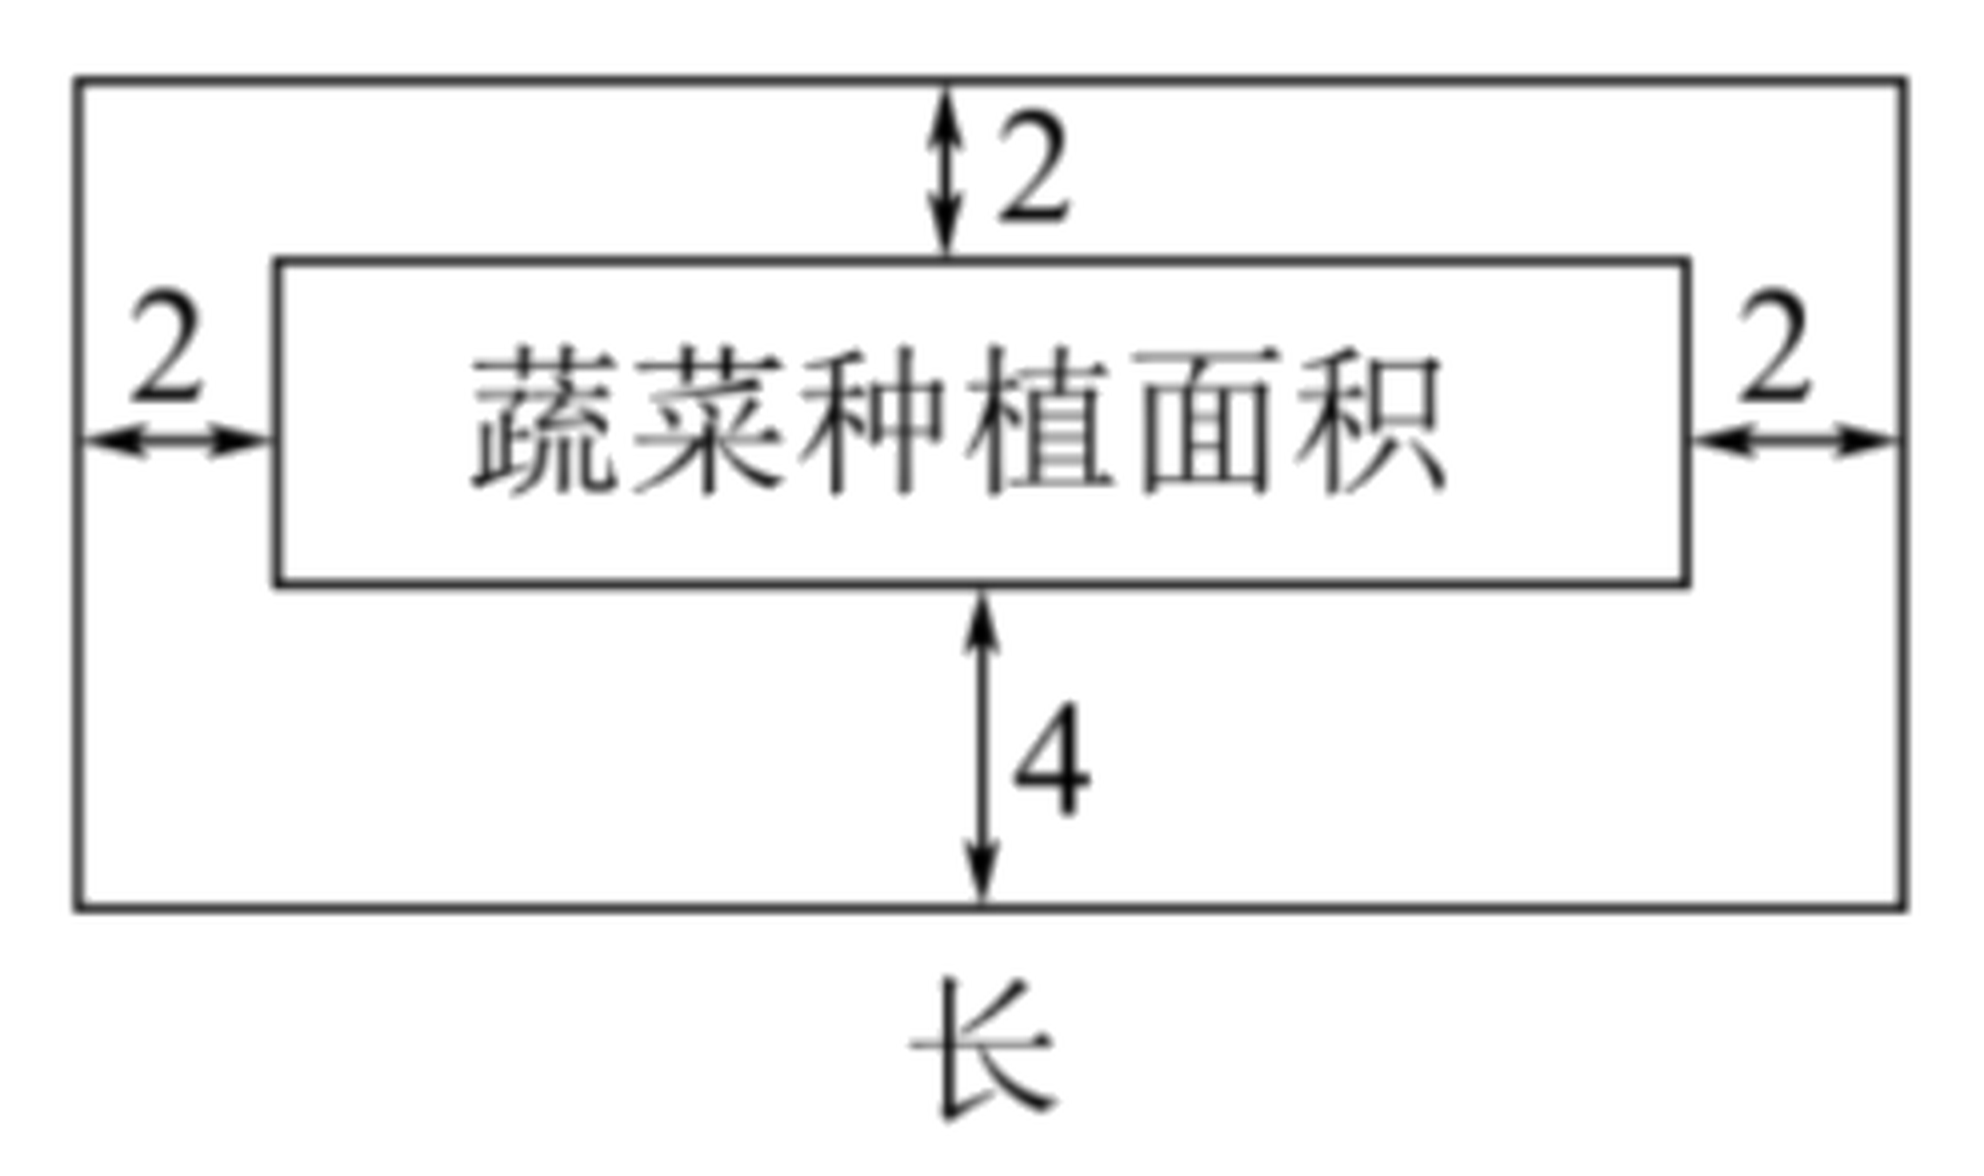
\includegraphics[width=0.45\textwidth]{figures/gao148_q20.png}
\end{center}

(1) 写出蔬菜的种植面积关于矩形温室的长之间的关系式.

(2) 当矩形温室的边长各为多少时，蔬菜的种植面积最大？最大种植面积是多少？

\ifanswer
\solbegin
\step{(1) 设蔬菜的种植面积为 $y\mathrm{m}^2$，矩形温室的长为 $x\mathrm{m}$，}
\step{则矩形温室的宽为 $\dfrac{600}{x}\mathrm{m}$，}
\step{种植蔬菜矩形的长为 $(x-4)\mathrm{m}$，宽为 $\left(\dfrac{600}{x}-6\right)\mathrm{m}$，}
\step{所以 $y=(x-4)\left(\dfrac{600}{x}-6\right)(4<x<100)$；}
\step{(2) 因为 $y=(x-4)\left(\dfrac{600}{x}-6\right)=624-\left(6x+\dfrac{2400}{x}\right)$，}
\step{因为 $6x+\dfrac{2400}{x}\geqslant2\sqrt{6x\cdot\dfrac{2400}{x}}=240$，}
\step{当且仅当 $6x=\dfrac{2400}{x}$，即 $x=20$ 时取等号，}
\step{所以 $y=624-\left(6x+\dfrac{2400}{x}\right)\leqslant624-240=384$.}
\step{即当矩形温室的一边长为 $20\mathrm{m}$，另一边长为 $30\mathrm{m}$ 时，}
\step{蔬菜的种植面积最大，最大为 $384\mathrm{m}^2$.}
\solend
\fi

% === Q21 ===：3 问、cases 块整体算一个印刷行；判别式高 \Delta；解析 19 行（末行续 09 页）
\item 二次函数 $f(x)=ax^2+bx+c$ 满足对任意的 $x\in\R$，$x-1\leqslant f(x)\leqslant x^2-x$ 恒成立.

(1) 求证：$f(1)$ 为定值；

(2) 若 $f(0)=-\dfrac{1}{4}$，求二次函数 $f(x)$ 的表达式；

(3) 求 $a+2b+5c$ 的取值范围.

\ifanswer
\solbegin
\step{(1) 对任意的 $x\in\R$，$x-1\leqslant f(x)\leqslant x^2-x$ 恒成立，则 $0\leqslant f(1)\leqslant0$，}
\step{所以 $f(1)=0$，为定值.}
\step{(2) 由(1)得 $a+b+c=f(1)=0$，由 $f(0)=-\dfrac{1}{4}$，得 $c=-\dfrac{1}{4}$，}
\step{则 $b=\dfrac{1}{4}-a$，$f(x)=ax^2+\left(\dfrac{1}{4}-a\right)x-\dfrac{1}{4}$，}
\step{不等式 $x-1\leqslant f(x)$ 可化为 $ax^2+\left(\dfrac{1}{4}-a\right)x-\dfrac{1}{4}\geqslant x-1$，}
\step{即 $ax^2-\left(a+\dfrac{3}{4}\right)x+\dfrac{3}{4}\geqslant0$，}
\step{一元二次不等式 $ax^2-\left(\dfrac{3}{4}+a\right)x+\dfrac{3}{4}\geqslant0$ 恒成立，则 $\begin{cases}a>0\\\Delta=\left(a+\dfrac{3}{4}\right)^2-3a\leqslant0\end{cases}$，}% 判别式原卷印等腰偏高粗三角 $\Delta$，照录（放大 08 页 q21_delta3.png／diag_band_q21.png 确认）
\step{解得 $a=\dfrac{3}{4}$，}
\step{此时 $f(x)=\dfrac{3}{4}x^2-\dfrac{1}{2}x-\dfrac{1}{4}$，$x^2-x-f(x)=\dfrac{1}{4}(x-1)^2\geqslant0$ 恒成立，}
\step{所以 $f(x)=\dfrac{3}{4}x^2-\dfrac{1}{2}x-\dfrac{1}{4}$.}
\step{(3) 由(1)得 $b=-a-c$，$f(x)=ax^2-(a+c)x+c=(ax-c)(x-1)$，}
\step{不等式 $x-1\leqslant f(x)$ 可化为 $(x-1)(ax-c-1)\geqslant0$，}
\step{一元二次不等式 $(x-1)(ax-c-1)\geqslant0$ 恒成立，则 $a>0$，}
\step{且方程 $(x-1)(ax-c-1)=0$ 有相等的实数根，因此 $c=a-1$，$a>0$，}
\step{不等式 $f(x)\leqslant x^2-x\Leftrightarrow(ax-c)(x-1)\leqslant x^2-x\Leftrightarrow(x-1)[(1-a)x+c]\geqslant0$，}
\step{同理 $1-a>0$，且方程 $(x-1)[(1-a)x+c]=0$ 有相等的实数根，}
\step{因此 $c=a-1$，$a<1$，从而 $c=a-1$，$b=1-2a$，$0<a<1$，}
\step{$a+2b+5c=a+2(1-2a)+5(a-1)=2a-3\in(-3,-1)$，}
\step{所以 $a+2b+5c$ 的取值范围是 $(-3,-1)$.}
\solend
\fi

\end{enumerate}

\end{document}
"
% 紧凑版：xelatex "\def\iscompact{1}% 高一148_新川中学_期中.tex
%   —— 高一上数学"2026-2027 年新川中学高一上期中"（试卷版/答案版/紧凑版）
% 试卷版：xelatex 高一148_新川中学_期中.tex
% 答案版：xelatex "\def\isanswer{1}% 高一148_新川中学_期中.tex
%   —— 高一上数学"2026-2027 年新川中学高一上期中"（试卷版/答案版/紧凑版）
% 试卷版：xelatex 高一148_新川中学_期中.tex
% 答案版：xelatex "\def\isanswer{1}\input{高一148_新川中学_期中.tex}"
% 紧凑版：xelatex "\def\iscompact{1}\input{高一148_新川中学_期中.tex}"
%
% ① 原始材料：微信公众号"魔都数学加油站"文章，连载"27学年高一148"，原文标题
% "27学年高一148——2026-2027年上海市新川中学高一上期中"（2026-11-21 推送）；
% 原文链接：https://mp.weixin.qq.com/s/Alhmwb3sSLQMp_wjzoAVyA 。
% 正文为 9 张 PNG 页（01/03/04/07/08/09 为 2560×3620，02/05/06 为 4762×6735，
% 同一篇各页分辨率混排，逐页按各自分辨率裁图核对，别按预览比例换算裁框）。
% 体例：混合体例讲评版——19 题中 Q4、Q5 只印【答案】、无【解析】；Q13 的答案"C"
% 直接印在题干括号内、无【答案】/【解析】段；其余 16 题印【解析】（逐题核实，见 ② ②）。
% 题目、答案、解析均据原图转录；卷面粉红色水印"魔都数学加油站"及公众号页脚未录入。
% 全卷插图清单（逐页通读 9 页确认）：4 幅题目配图，均三版都出、均非【解析】内配图：
%   · Q12 幂函数曲线族图（03 页右侧：x/y 轴、O、A(1,0)、B(0,1)、M、N 与两族
%     y=x^α／y=x^β 曲线、线段 AB、虚线），题干"（如图）"处，裁 figures/gao148_q12.png；
%   · Q15 四条指数函数曲线图（04 页右侧：①②③④ 四曲线同过 (0,1)、x/y 轴、O、
%     y 轴刻度 1），题干"如图"处，裁 figures/gao148_q15.png；
%   · Q16 关于 y 轴对称的幂函数曲线图（04 页右下：x/y 轴、O、两支上翘曲线），
%     题干"如图所示"处，裁 figures/gao148_q16.png；
%   · Q20 矩形蔬菜温室示意图（07 页右侧：大矩形＋内框"蔬菜种植面积"＋2/2/4
%     通道标注＋"长"），题干处，裁 figures/gao148_q20.png；
%   其余各页逐页确认无其它题目配图、无【解析】内配图、无表格，亦无"题干写如图而
%   源码漏图"一处；Q19 解析行末的虚线"----N 分"为评分档（非图），Q18／Q21 的
%   cases 块为数学块（非图）。4 图均取自原卷截图，去粉色水印、去色、4× LANCZOS 放大。
%
% 卷首标题：原卷印作"2026-2027 年新川中学高一上期中"，年份区间按全稿惯例排 en dash；
% 原卷卷面未印副标题，本稿按同期中卷（高一140／141／143／144／145／146／147）知识模块
% 口径补出"集合与常用逻辑用语、不等式、函数"。
%
% 题号体例（逐页核实定稿）：本卷共 19 题——一、填空题 3—12（10 题）、
% 二、选择题 13—16（4 题）、三、解答题 17—21（5 题）。
% 三节分别 \setcounter{enumi}{2}／{12}／{16}。原卷从第 3 题起、无第 1、2 题，
% 本稿保留原题号；全卷无附加题节、无 Q22（Q21 解析末行"所以 a+2b+5c 的取值范围是
% (-3,-1)."为全卷收尾，09 页下半仅水印、无正文）。
%
% ② 与原卷的排版差异：
%   ① 原文从第 3 题起，本稿保留原题号；共 19 题三节；
%   ② 混合体例逐题核实：Q4（反证法"假设的内容"）、Q5 只印【答案】、无【解析】，
%      按 高一140 第 5 题／高一145 Q3 成例提 \ans{}、不补造解析；Q13 答案"C"直接
%      印在题干括号内（" ( C ) "）、全卷无该题【答案】/【解析】段，按 高一84 Q13／
%      高一37 Q13／高一53 Q13 成例括号 \mbox{（\quad）} 留空、另提 \ans{$C$}；
%      其余 16 题印【解析】、用 \solbegin…\solend，选择题答案在解析末句"故选 X"
%      （Q14 选 D、Q15 选 B、Q16 选 D，逐个放大原图核实）、题干括号留空、不另提
%      \ans{}；答案版【答案】/【解析】标记数 = 19（3 个 \ans ＋ 16 个 \solbegin）
%      = 全卷题数；
%   ③ 原卷卷面未印副标题，本稿按知识模块口径补出；
%   ④ 原卷填空横线按全稿惯例排 \blankline[4.4em]；选择题括号排 \mbox{（\quad）}、
%      选项段前按惯例加 \keepwithprev；Q13／Q16 四选项为两行两列、Q14／Q15 选项
%      为一行，照原卷分行；解答题不留作答区、不加 \anspace（原卷为讲评版，
%      与 129／131／132／133／136／140／141／143／144／145／146 同）；
%   ⑤ 数集：Q11"在 R 上定义运算"、Q13"x、y∈R"、Q16"p、q∈Z"、Q17"a∈R"
%      "U=R"、Q19"m∈R"、Q21"x∈R" 原卷印斜体 R/Z，按全稿惯例统一改 \R／\Z
%      （本卷未出现 N，\N^* 无对应处）；绝对值排 \lvert…\rvert（Q9／Q14），
%      集合描述竖线排 \mid（Q17）；不等号按全稿惯例排 \leqslant／\geqslant；
%      补集照原卷上划线排 \overline{B}（Q17 题干 1 处＋解析 3 处）；空集
%      \varnothing（Q17 题干 1 处＋解析 2 处）；\subset（Q3 题干 {a}⊂M）与
%      \subseteq（Q3 题干 M⊆{a,b,c,d}）逐处照录不统一（放大 01 页 q3_subset.png）；
%   ⑥ 子题标号 (1)(2)(3) 半角括号照录；圈数字 ①—⑥ 在文本模式（Q14 六个结论、
%      Q15 曲线编号与其解析、Q14 解析"对①…对⑥"），按 common.sty 划入 CJK 字符类
%      渲染；cases 块整体算一个印刷行；\left…\right 不得拆到不同 $…$ 组；
%      单位 m／m² 排 \mathrm{m}／\mathrm{m}^2（Q20，原卷印正体 m）；
%   ⑦ 题干／解析中的中文弯引号按原卷照录：Q4" ab 可以被 5 整除，那么 a、b 中
%      至少有一个能被 5 整除 "（开引号后有空格、闭引号后空格接"时"）、
%      Q13" x=0 "" xy=0 "（引号内空格），注释内一律 ASCII 引号；
%   ⑧ 半角逗号在数学组之间是全稿惯例、非笔误（Q3"{a,b,c,d}"、Q6"$x,y$"
%      "$x=\frac13,y=\frac16$"、Q10、Q11"$a=-2,b=-1"、Q12"$\alpha=\log..,\beta=..$"、
%      Q14"$a+b<0,a-b<0$"、Q17、Q19"$x_1+x_2=-6,x_1\cdot x_2=7$"、Q20、Q21 等），
%      逐处照录别改全角；行末西文句点照录为 ASCII `.`；行中全角逗号／顿号照录；
%   ⑨ "图像／图象"逐处放大核：全卷 9 处均印"图象"（象，无亻）、未见"图像"，
%      逐处照录未统一改动（Q8 题干/解析各 1、Q12 题干 2、Q15 题干 1／解析 2、
%      Q16 题干 1／解析 1；放大 02/03/04/05 页 /tmp/gao148/zoom/my_wide_a.png、
%      my_wide_b.png 与宋体参考"象／像"并排确认）；
%   ⑩ 判别式 Δ/△ 混用是照录项：Q11 解析"△=1−4(−a²+a+1)<0"印扁等边空心
%      三角 \triangle；Q19 解析"Δ=36m²−4(9m−2)>0"、Q21 解析 cases 块
%      "Δ=(a+3/4)²−3a≤0" 两处印等腰偏高粗三角 \Delta，逐处放大判断、照录
%      不统一（参照 高一142／144／145 头注④口径，详见 ④）；
%   ⑪ 一条 \step = 原卷解析的一个印刷行，cases 块整体算一个印刷行；别把原卷折行
%      并起来、别把一行拆多条。Q3 六行、Q7 五行（01 页末首行＋02 页顶四行）、
%      Q9 七行、Q11 五行、Q14 八行（对② 的两行公式各占一印刷行）、Q17 八行、
%      Q18 六行、Q19 九行（7 处评分档附在行末）、Q20 十行、Q21 十九行
%      均按印刷行逐条断，不丢行；
%   ⑫ 配图：4 幅均为题目配图（三版都出），放 \item 内题干之后 \begin{center}；
%      大图块加 \needvspace 守卫把整块推走（守卫放 \item 之前，见 高一145 Q14/Q20
%      成例与切页审计 B 类坑）；三版切页审计均"合计异常：无"；
%   ⑬ 跨页续印按题合并：Q3/4/5 在 01 页；Q6 题干＋解析在 01 页；Q7 题干在 01 页
%      末、解析首行在 01 页末续 02 页顶四行；Q8/9/10 在 02 页（Q9 解析续 02 页下半、
%      Q10 题干与解析前 2 行在 02 页末）；Q10 解析末行续 03 页顶；Q11/12 在 03 页、
%      "二、选择题"标题与 Q13/14 题干在 03 页下半；Q13 无解析；Q14 解析在 04 页顶、
%      Q15 题干＋图＋选项＋解析在 04 页、Q16 题干＋图在 04 页末；Q16 选项＋解析＋
%      "三、解答题"标题＋Q17 题干＋解析在 05 页、Q18 题干首句在 05 页末；Q18 题干
%      续＋解析、Q19 题干＋解析前 5 行在 06 页；Q19 解析续 4 行＋Q20 题干＋图＋
%      解析（10 行全部）在 07 页，末行"蔬菜的种植面积最大，最大为 384m²."收尾；
%      Q21 题干＋解析前 18 行在 08 页；Q21 解析末行"所以 a+2b+5c 的取值范围是
%      (-3,-1)."在 09 页上半（09 页下半仅水印、无正文）。本稿按题连排，不丢行、
%      不并折行；
%   ⑭ 原卷解析内无红色"法一／法二"之类小标题，故本卷无 \stepm；水印
%      "魔都数学加油站"红色不录入；Q19 解析 7 处评分档（1/2/3/2/2/2/2 分）
%      原卷在行末印一串虚线，本稿照 高一54／64 成例排 \dots\dots N 分，
%      分值逐处照录、位置不变。
%
% ③ 行数复核：一条 \step／\stepm = 原卷解析的一个印刷行，cases 块作一个印刷行计。
%   逐题数（主会话逐页核对定稿）：Q3：6；Q4：0（只印【答案】、提 \ans{}）；
%   Q5：0（只印【答案】、提 \ans{}）；Q6：2；Q7：5；Q8：2；Q9：7；Q10：3；
%   Q11：5；Q12：2；Q13：0（答案印在题干括号内、另提 \ans{}）；Q14：8；Q15：5；
%   Q16：2；Q17：8；Q18：6；Q19：9；Q20：10；Q21：19。
%   合计 99 条 \step（本卷无 \stepm：解析内无红色"法一／法二"类小标题），
%   与原卷逐题印刷行相等。全卷 16 题设 \solbegin…\solend ＋ 3 处 \ans{}，
%   答案版【答案】/【解析】标记数 = 19 = 全卷题数。
%
% ④ 判别式／子集符号结论（逐处放大原图照录、不得统一，主会话像素级复核）：
%   判别式全卷 3 处，两形混用逐处照录不统一（参照 高一142／144／145 头注④口径）：
%     · Q11 解析"△=1−4(−a²+a+1)<0" 原卷印扁等边空心三角（宽>高、细线），
%       照录 \triangle（放大 03 页 /tmp/gao148/zoom/q11_delta3.png、
%       delta_montage.png 确认）；
%     · Q19 解析"Δ=36m²−4(9m−2)>0" 原卷印等腰偏高粗三角（高>宽），
%       照录 \Delta（放大 07 页 /tmp/gao148/zoom/q19_delta3.png 确认）；
%     · Q21 解析 cases 块"Δ=(a+3/4)²−3a≤0" 原卷印等腰偏高粗三角（高>宽），
%       照录 \Delta（放大 08 页 /tmp/gao148/zoom/q21_delta3.png 确认）。
%   子集／补集：Q3 题干"{a}⊂M⊆{a,b,c,d}" 前者印单线 ⊂、无下划线，照录 \subset；
%     后者印带下划线 ⊆，照录 \subseteq（放大 01 页 /tmp/gao148/zoom/q3_subset.png
%     确认）；Q17 题干 1 处＋解析 3 处共 4 处 \overline{B} 照原卷上划线
%     （B 上横线、非 C_U B）；空集 \varnothing 3 处（Q17 题干 1 处、解析 2 处）；
%     Q17 集合描述竖线 \mid；数集 \R／\Z 归一见 ② ⑤。
%
% ⑤ 存疑照录（放大原图确认，照录未改、正文对应处另有 % 注）：
%   1. Q3 解析末行"所以 M 一共有 3+3+1+1=8 个" 原卷印 $3+3+1+1=8$，按上文
%      四行应为 $1+3+3+1=8$（疑为原卷加数顺序笔误，和仍为 8），放大 01 页
%      /tmp/gao148/zoom/my_q3_sol.png 确认，照录未改。
%   2. Q13 答案"C"直接印在题干括号内、全卷无该题【答案】/【解析】段，按
%      高一84 Q13 成例括号留空、另提 \ans{$C$}（见 ② ②），未补造解析。
%   3. Q19 解析 7 处评分档（"----N 分"）原卷印一串虚线，本稿照 高一54／64
%      成例排 \dots\dots N 分，分值逐处照录、位置不变。
%   4. 判别式 Q11 扁 \triangle 与 Q19／Q21 高 \Delta 两形混用，逐处照录不统一（见 ④）。
%   5. "图像／图象"全卷 9 处均印"图象"、未见"图像"（见 ② ⑨），逐处放大核实照录，
%      未统一改动。
%   全卷除此 5 类外未发现其它笔误／自相矛盾处。
%
% ⑥ 跨页续印按题合并说明：见 ② ⑬。
%
\documentclass[a4paper,11pt]{article}
\usepackage{common}

\begin{document}

\examtitlest[3]{2026--2027 年新川中学高一上期中}{集合与常用逻辑用语、不等式、函数}

\bigsec{一、填空题}

\begin{enumerate}
\setcounter{enumi}{2}

% === Q3 ===：题干 {a}⊂M⊆{a,b,c,d} 两个子集符号逐处照录；解析 6 行
\item 满足 $\{a\}\subset M\subseteq\{a,b,c,d\}$ 的集合 $M$ 有\blankline[4.4em]个.

\ifanswer
\solbegin
\step{$M$ 是 $\{a,b,c,d\}$ 的子集，但必含有元素 $a$，}
\step{当 $M$ 中只一个元素时，$M=\{a\}$ 只有 1 个；}
\step{当 $M$ 中有二个元素时，$M$ 有 3 个；}
\step{当 $M$ 中有三个元素时，$M$ 有 3 个；}
\step{当 $M$ 中有四个元素时，$M$ 有 1 个；}
\step{所以 $M$ 一共有 $3+3+1+1=8$ 个.}% 原卷印 $3+3+1+1=8$（按上文四行应为 $1+3+3+1$），疑为加数顺序笔误，照录未改（放大 01 页 my_q3_sol.png）
\solend
\fi

% === Q4 ===：原卷只印【答案】、无【解析】，按 高一140 第 5 题成例提 \ans{}；弯引号与空格照录
\item 用反证法证明命题 “ $ab$ 可以被 5 整除，那么 $a$、$b$ 中至少有一个能被 5 整除” 时假设的内容应该是\blankline[4.4em].

\ifanswer
\ans{$a$、$b$ 都不能被 5 整除}
\fi

% === Q5 ===：原卷只印【答案】 $[-2,1)$、无【解析】，提 \ans{}
\item 不等式 $\dfrac{x+2}{x-1}\leqslant0$ 的解集为\blankline[4.4em].

\ifanswer
\ans{$[-2,1)$}
\fi

% === Q6 ===：解析 2 行；半角逗号在数学组之间照录
\item 设 $x,y\in(0,+\infty)$，且 $x+4y=1$，则 $\dfrac{1}{x}+\dfrac{1}{y}$ 的最小值为\blankline[4.4em].

\ifanswer
\solbegin
\step{因为 $\dfrac{1}{x}+\dfrac{1}{y}=(x+4y)\left(\dfrac{1}{x}+\dfrac{1}{y}\right)=5+\dfrac{4y}{x}+\dfrac{x}{y}\geqslant5+2\sqrt{\dfrac{4y}{x}\cdot\dfrac{x}{y}}=9$，}
\step{当且仅当 $\dfrac{4y}{x}=\dfrac{x}{y}$，即 $x=2y$，即 $x=\dfrac{1}{3},y=\dfrac{1}{6}$ 时取等号，故最小值为 9.}
\solend
\fi

% === Q7 ===：题干在 01 页末、解析首行在 01 页末续 02 页顶四行；解析 5 行
\item 若不等式 $x^2+ax+b<0$ 的解集为 $(-3,-1)$，则不等式 $bx^2+ax+1\leqslant0$ 的解集为\blankline[4.4em].

\ifanswer
\solbegin
\step{不等式 $x^2+ax+b<0$ 的解集为 $(-3,-1)$，}
\step{所以方程 $x^2+ax+b=0$ 的两个实数根为 $-3$ 和 $-1$，}
\step{由根与系数的关系得 $a=4$，$b=3$，}
\step{故 $bx^2+ax+1\leqslant0$ 可化为 $3x^2+4x+1\leqslant0$，解得 $-1\leqslant x\leqslant-\dfrac{1}{3}$，}
\step{所求不等式 $bx^2+ax+1\leqslant0$ 的解集为 $\left[-1,-\dfrac{1}{3}\right]$.}
\solend
\fi

% === Q8 ===："图象"照录；解析 2 行
\item 函数 $y=a^{x-2}+2(a>0,a\ne1)$ 的图象必经过定点\blankline[4.4em].

\ifanswer
\solbegin
\step{令 $x-2=0$，得 $x=2$，则 $y=a^0+2=3$，}
\step{所以函数 $y=a^{x-2}+2$ 的图象过定点 $(2,3)$.}
\solend
\fi

% === Q9 ===：解析 7 行；首句末西文句点照录
\item 不等式 $\lvert x+3\rvert+\lvert a-x\rvert>6$ 对一切实数 $x$ 恒成立，则实数 $a$ 的取值范围为\blankline[4.4em].

\ifanswer
\solbegin
\step{$\lvert x+3\rvert$ 表示 $x$ 到 $-3$ 的距离，$\lvert a-x\rvert$ 表示 $x$ 到 $a$ 的距离.}
\step{所以它们的和为 $x$ 到 $-3$ 和 $x$ 到 $a$ 的距离之和，}
\step{当 $x$ 位于 $-3$ 和 $a$ 之间时，距离和取得最小值，}
\step{即两点之间的距离 $\lvert a-(-3)\rvert=\lvert a+3\rvert$，}
\step{若最小值 $\lvert a+3\rvert>6$，则原式对所有 $x$ 恒成立.}
\step{解得 $a+3>6$ 或 $a+3<-6$，即 $a>3$ 或 $a<-9$，}
\step{故 $a\in(3,+\infty)$ 或 $a\in(-\infty,-9)$.}
\solend
\fi

% === Q10 ===：题干与解析前 2 行在 02 页末、解析末行续 03 页顶；解析 3 行
\item 已知 $2^a=3$，$\log_3 5=b$，则 $\log_{15}20=$\blankline[4.4em]（用 $a$、$b$ 表示）.

\ifanswer
\solbegin
\step{因为 $2^a=3$，所以 $a=\log_2 3=\dfrac{\lg3}{\lg2}$，又 $\log_3 5=b=\dfrac{\lg5}{\lg3}$，}
\step{所以 $\lg3=a\lg2$，$\lg5=b\lg3=ba\lg2$，}
\step{则 $\log_{15}20=\dfrac{2\lg2+\lg5}{\lg3+\lg5}=\dfrac{2\lg2+ab\lg2}{a\lg2+ab\lg2}=\dfrac{2+ab}{a+ab}$.}
\solend
\fi

% === Q11 ===：在 \R 上定义运算 \otimes；判别式扁 \triangle 照录；解析 5 行
\item 在 $\R$ 上定义运算 $\otimes:x\otimes y=x(1-y)$，若不等式 $(x-a)\otimes(x+a)<1$ 对任意实数 $x$ 恒成立，则 $a$ 的取值范围是\blankline[4.4em].

\ifanswer
\solbegin
\step{由题意得不等式 $(x-a)\otimes(x+a)<1$ 对任意实数 $x$ 恒成立，}
\step{即不等式 $(x-a)(1-x-a)<1$ 对任意实数 $x$ 恒成立，}
\step{即 $x^2-x-a^2+a+1>0$ 对任意实数 $x$ 恒成立，}
\step{所以 $\triangle=1-4(-a^2+a+1)<0$，解得 $-\dfrac{1}{2}<a<\dfrac{3}{2}$，}% 判别式原卷印扁等边空心三角 $\triangle$，照录（放大 03 页 q11_delta3.png 确认）
\step{所以实数 $a$ 的取值范围为 $\left(-\dfrac{1}{2},\dfrac{3}{2}\right)$.}
\solend
\fi

% === Q12 ===：题目配图（幂函数曲线族，三版都出）；"图象"照录；解析 2 行
\needvspace{8cm}
\item 幂函数 $y=x^\alpha$，当 $\alpha$ 取不同的正数时，在区间 $[0,1]$ 上它们的图象是一族美丽的曲线（如图）. 设点 $A(1,0)$，$B(0,1)$，连接 $AB$，线段 $AB$ 恰好被其中的两个幂函数 $y=x^\alpha$，$y=x^\beta$ 的图象三等分，即有 $BM=MN=NA$，那么 $\alpha\beta=$\blankline[4.4em].

\begin{center}
% 幂函数曲线族图取 03 页右侧，去粉色水印、去色、4× LANCZOS 放大；三版都出
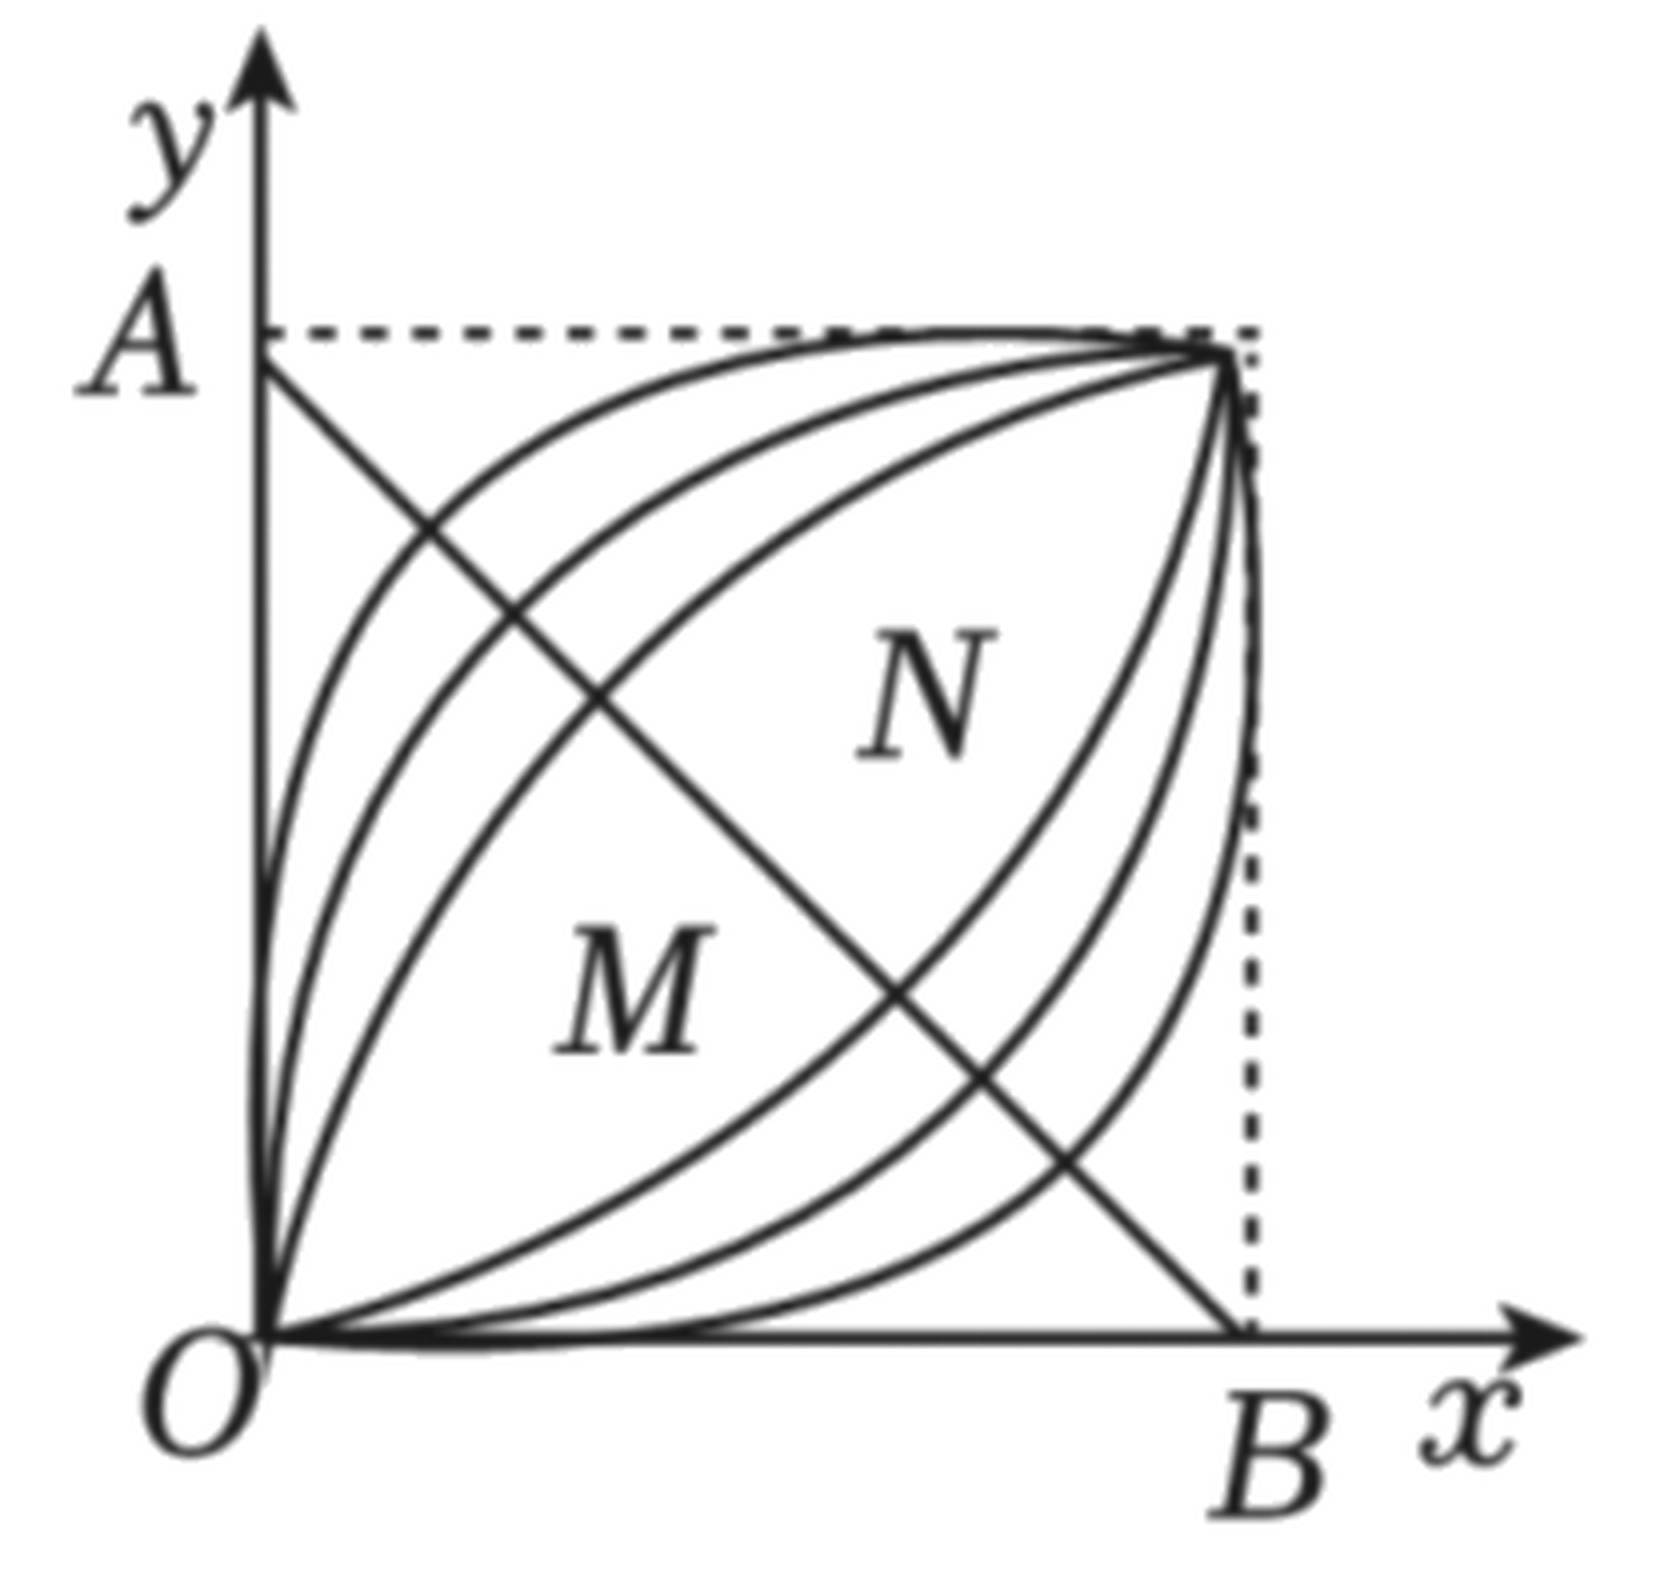
\includegraphics[width=0.40\textwidth]{figures/gao148_q12.png}
\end{center}

\ifanswer
\solbegin
\step{$BM=MN=NA$，点 $A(1,0)$，$B(0,1)$，所以 $M\left(\dfrac{1}{3},\dfrac{2}{3}\right)$，$N\left(\dfrac{2}{3},\dfrac{1}{3}\right)$，}
\step{分别代入 $y=x^\alpha$，$y=x^\beta$，$\alpha=\log_{\frac{2}{3}}\dfrac{1}{3},\beta=\log_{\frac{1}{3}}\dfrac{2}{3}$，$\alpha\beta=\log_{\frac{1}{3}}\dfrac{2}{3}\cdot\log_{\frac{2}{3}}\dfrac{1}{3}=1$.}
\solend
\fi

\end{enumerate}

\bigsec{二、选择题}

\begin{enumerate}
\setcounter{enumi}{12}

% === Q13 ===：答案"C"直接印在题干括号内、全卷无该题【答案】/【解析】段，按 高一84 Q13 成例括号留空、另提 \ans{$C$}；弯引号含空格
\item 若 $x$、$y\in\R$，则 “ $x=0$ ” 是 “ $xy=0$ ” 的\mbox{（\quad）}

\keepwithprev
A. 充要条件\qquad\qquad B. 必要不充分条件

C. 充分不必要条件\qquad\qquad D. 既不充分也不必要条件

\ifanswer
\ans{$C$}
\fi

% === Q14 ===：六个结论（圈数字在文本模式）、四选项一行；解析 8 行（对② 的两行公式各占一印刷行）
\item 若 $a<b<0$，下面有六个结论：① $a^2>b^2$；② $a^3<b^3$；③ $\dfrac{1}{a}<\dfrac{1}{b}$；④ $\dfrac{a}{b}>1$；⑤ $\dfrac{1}{a-b}>\dfrac{1}{a}$；⑥ $\lvert a\rvert>-b$. 其中正确的个数是\mbox{（\quad）}

\keepwithprev
A. 1\qquad\qquad B. 2\qquad\qquad C. 3\qquad\qquad D. 4

\ifanswer
\solbegin
\step{对①：$a^2-b^2=(a+b)(a-b),a+b<0,a-b<0$，故 $a^2-b^2>0$，正确；}
\step{对②：$a^3-b^3=(a-b)(a^2+ab+b^2)=(a-b)\left[\left(a+\dfrac{1}{2}b\right)^2+\dfrac{3}{4}b^2\right],a-b<0$，}
\step{$\left(a+\dfrac{1}{2}b\right)^2+\dfrac{3}{4}b^2>0$，故 $a^3-b^3<0$，正确；}
\step{对③：取 $a=-2,b=-1$，则 $\dfrac{1}{a}=-\dfrac{1}{2},\dfrac{1}{b}=-1,\dfrac{1}{a}>\dfrac{1}{b}$，错误；}
\step{对④：$\dfrac{a}{b}-1=\dfrac{a-b}{b},a-b<0,b<0$，故 $\dfrac{a}{b}-1>0$，正确；}
\step{对⑤：取 $a=-2,b=-1$，则 $\dfrac{1}{a-b}=-1,\dfrac{1}{a}=-\dfrac{1}{2},\dfrac{1}{a-b}<\dfrac{1}{a}$，错误；}
\step{对⑥：要证 $\lvert a\rvert>-b$，即 $-a>-b$，即 $a<b$，正确；}
\step{故选 $D$.}
\solend
\fi

% === Q15 ===：题目配图（四条指数函数曲线，三版都出），\needvspace 守卫放 \item 之前；"图象"照录；解析 5 行
\needvspace{8cm}
\item 如图，曲线①②③④分别是指数函数 $y=a^x$，$y=b^x$，$y=c^x$，$y=d^x$ 的图象，则实数 $a$、$b$、$c$、$d$ 的大小关系为\mbox{（\quad）}

\keepwithprev
A. $a<b<c<d$\qquad B. $b<a<d<c$\qquad C. $d<c<b<a$\qquad D. $c<d<a<b$

\begin{center}
% 四条指数函数曲线图取 04 页右侧，去粉色水印、去色、4× LANCZOS 放大；三版都出
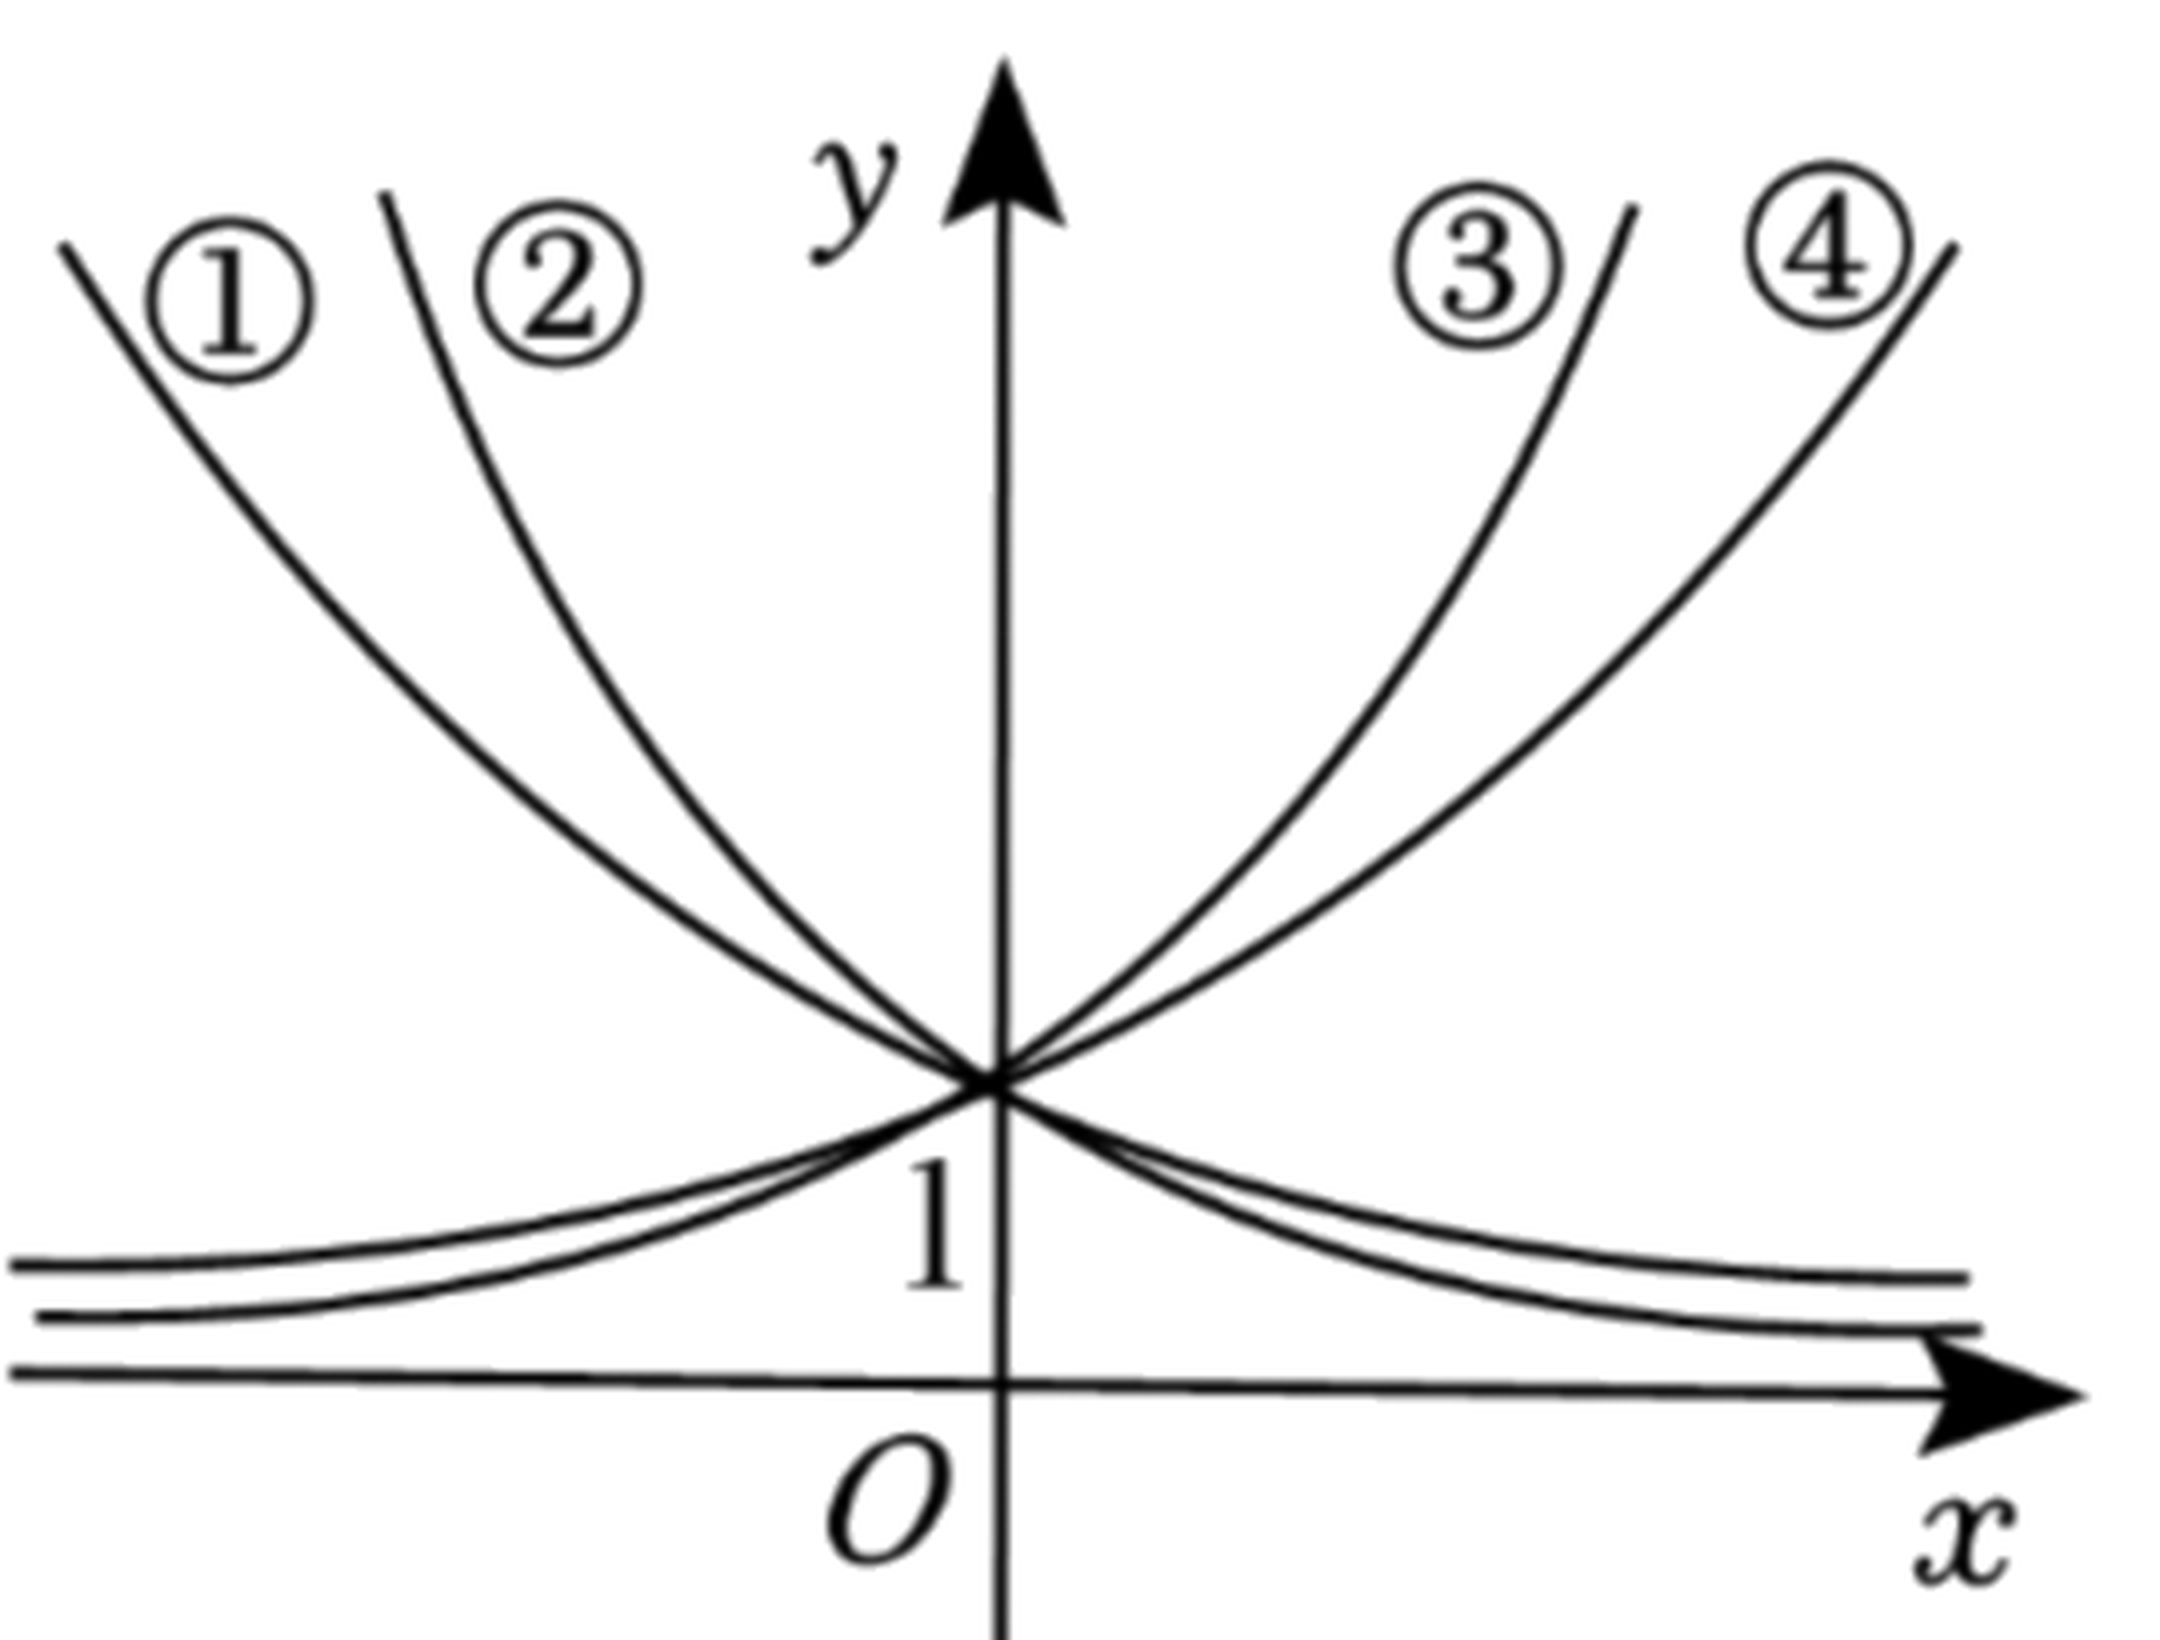
\includegraphics[width=0.40\textwidth]{figures/gao148_q15.png}
\end{center}

\ifanswer
\solbegin
\step{由函数图象得函数① $y=a^x$；② $y=b^x$ 为减函数，且 $x=1$ 时，$b^1<a^1$，}
\step{所以 $0<b<a<1$，}
\step{由函数图象得函数③ $y=c^x$；④ $y=d^x$ 为增函数，且 $x=1$ 时，$c^1>d^1$，}
\step{所以 $c>d>1$，}
\step{所以 $b<a<d<c$. 故选 $B$.}
\solend
\fi

% === Q16 ===：题目配图（关于 y 轴对称的幂函数曲线，三版都出），\needvspace 守卫放 \item 之前；$p$、$q\in\Z$；"图象"照录；解析 2 行
\needvspace{8cm}
\item 已知幂函数 $y=x^{\frac{p}{q}}$（$p$、$q\in\Z$ 且 $p$、$q$ 互质）的图象关于 $y$ 轴对称，如图所示，则\mbox{（\quad）}

\keepwithprev
A. $p$、$q$ 均为奇数，且 $\dfrac{p}{q}>0$\qquad\qquad B. $q$ 为偶数，$p$ 为奇数，且 $\dfrac{p}{q}<0$

C. $q$ 为奇数，$p$ 为偶数，且 $\dfrac{p}{q}>0$\qquad\qquad D. $q$ 为奇数，$p$ 为偶数，且 $\dfrac{p}{q}<0$

\begin{center}
% 关于 y 轴对称的幂函数曲线图取 04 页右下，去粉色水印、去色、4× LANCZOS 放大；三版都出
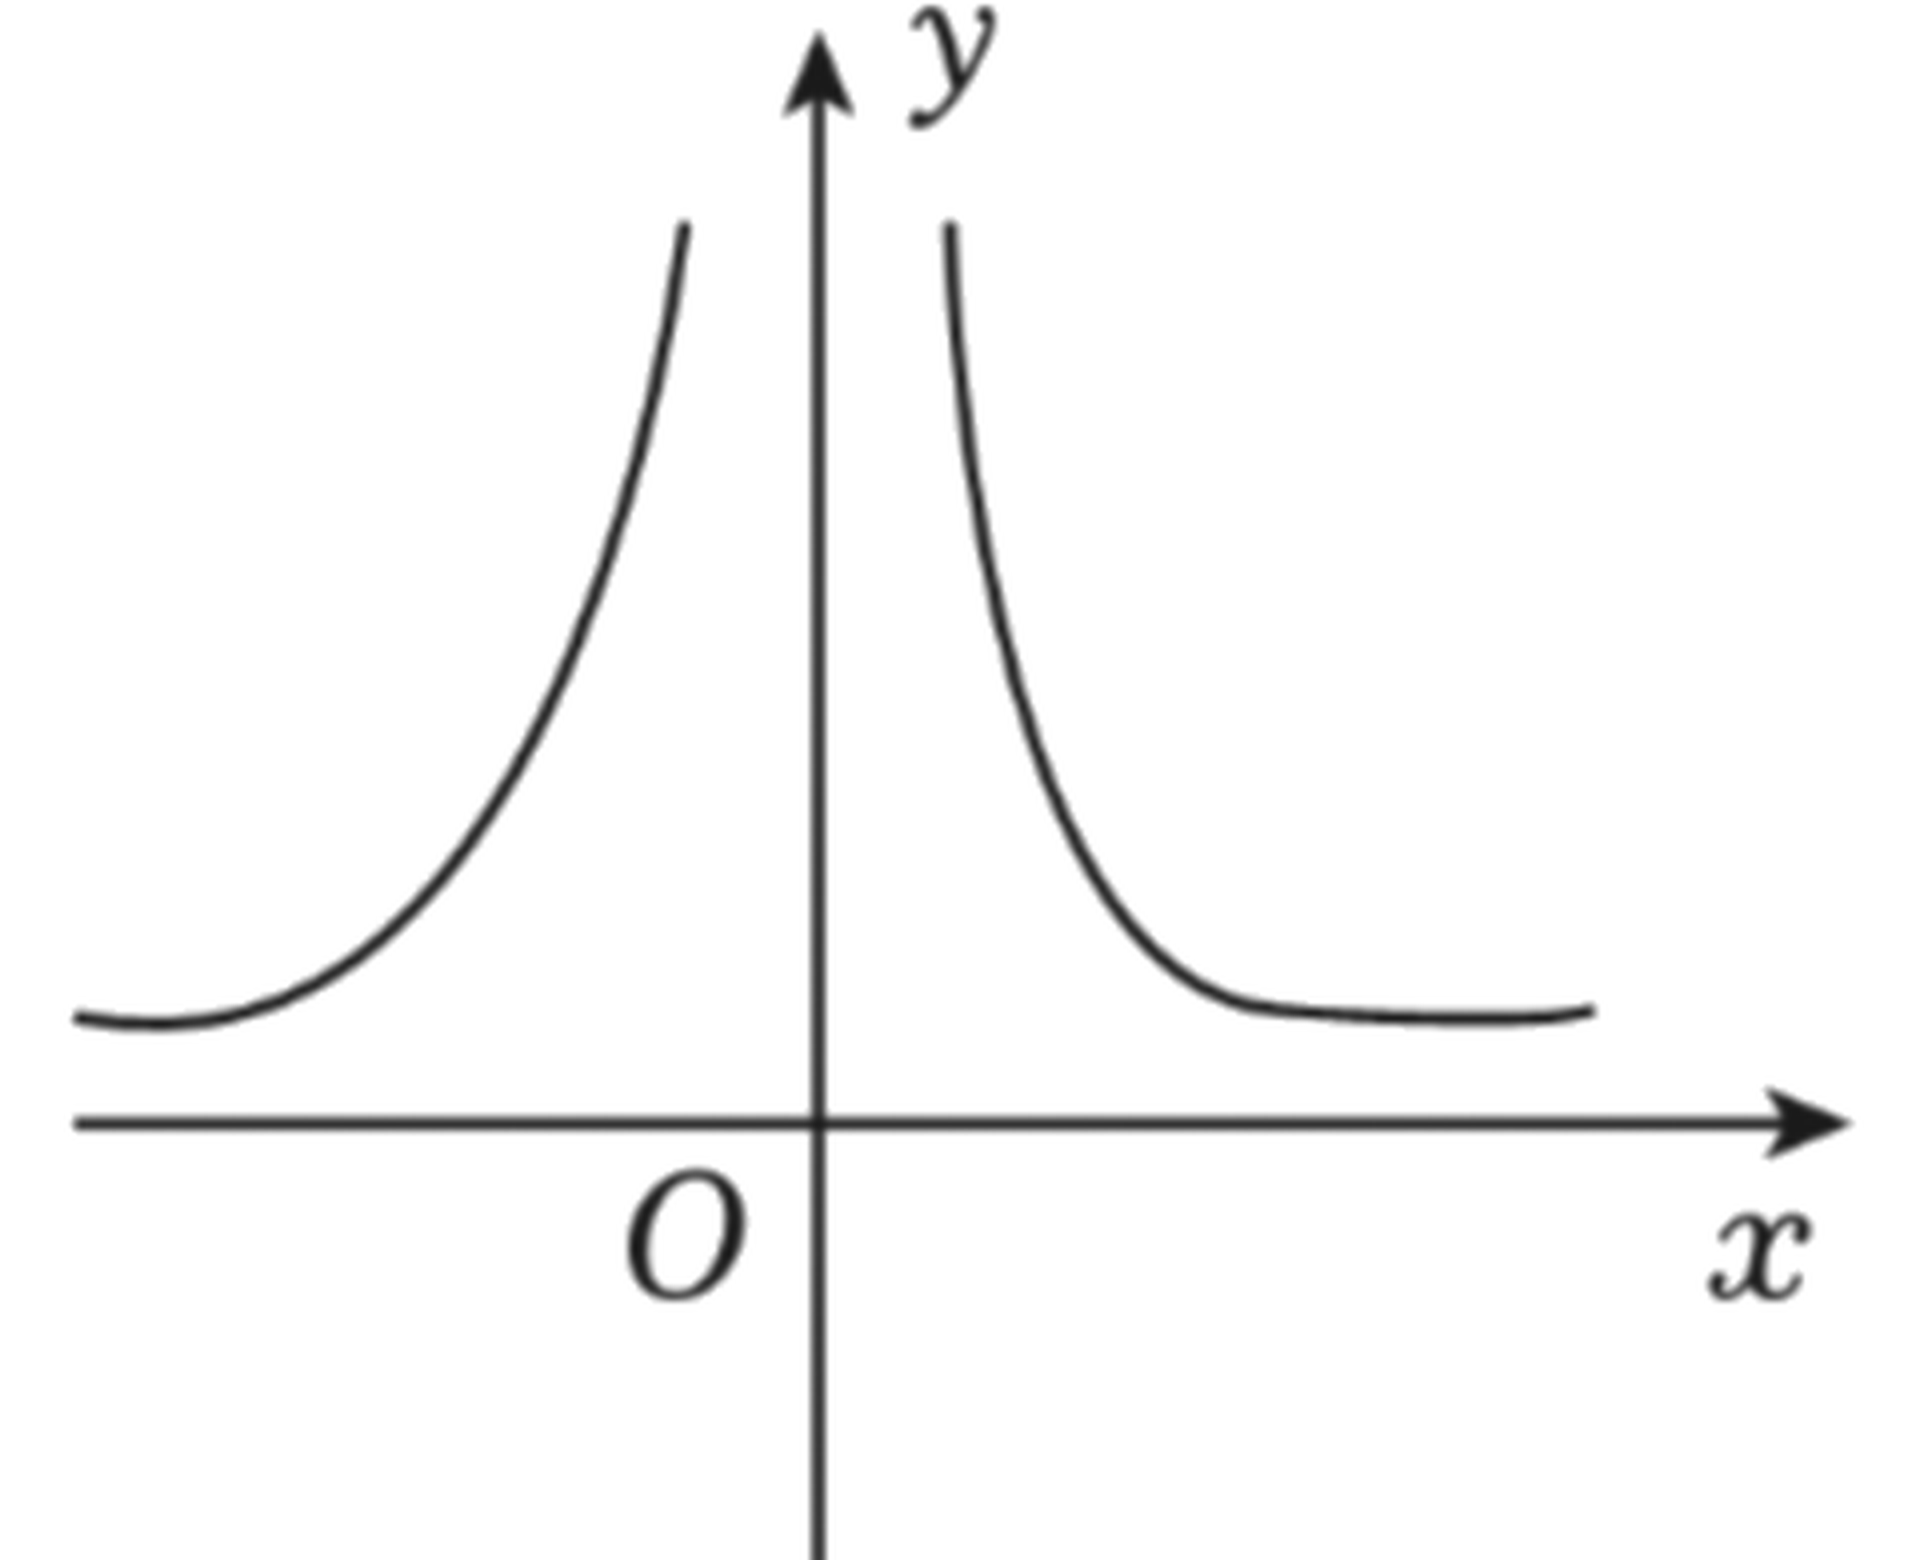
\includegraphics[width=0.36\textwidth]{figures/gao148_q16.png}
\end{center}

\ifanswer
\solbegin
\step{因为函数为偶函数，所以 $p$ 为偶数，且由图象形状判定 $\dfrac{p}{q}<0$.}
\step{又 $p$、$q$ 互质，所以 $q$ 为奇数. 故选 $D$.}
\solend
\fi

\end{enumerate}

\bigsec{三、解答题}

\begin{enumerate}
\setcounter{enumi}{16}

% === Q17 ===：\overline{B}／\varnothing／\R／\mid 逐处照录；解析 8 行
\item 已知集合 $A=\left\{x\mid \dfrac{5}{2x+1}>1\right\}$，$B=\{x\mid x^2+(a+3)x+3a<0,a\in\R\}$.

(1) 求 $A$.

(2) 若全集 $U=\R$，且 $A\cap\overline{B}=\varnothing$，求实数 $a$ 的取值范围.

\ifanswer
\solbegin
\step{(1) $\dfrac{5}{2x+1}>1$，即 $\dfrac{5}{2x+1}-1>0$，即 $\dfrac{4-2x}{2x+1}>0$，即 $(2x+1)(x-2)<0$，}
\step{解得 $-\dfrac{1}{2}<x<2$，所以 $A=\left(-\dfrac{1}{2},2\right)$；}
\step{(2) $x^2+(a+3)x+3a<0$，即 $(x+3)(x+a)<0$，}
\step{全集 $U=\R$，且 $A\cap\overline{B}=\varnothing$，}
\step{当 $a<3$ 时，解得 $-3<x<-a$，则 $\overline{B}=(-\infty,-3)\cup(-a,+\infty)$，}
\step{此时 $-a\geqslant2$，解得 $a\leqslant-2$，}
\step{当 $a\geqslant3$ 时，不满足 $A\cap\overline{B}=\varnothing$，}
\step{故实数 $a$ 的取值范围是 $(-\infty,-2]$.}
\solend
\fi

% === Q18 ===：cases 块整体算一个印刷行；解析 6 行
\item 已知幂函数经过点 $(2,4)$.

(1) 当 $x=\dfrac{1}{2}$ 时，求函数的值；

(2) 是否存在实数 $m$、$n$，使得该函数在区间 $[m,n]$ 上最小值为 $6m-8$，最大值为 $6n-8$？若存在，求出 $m$、$n$ 的值，若不存在，请说明理由.

\ifanswer
\solbegin
\step{(1) 设幂函数的解析式是 $y=x^\alpha$，则 $2^\alpha=4$，解得 $\alpha=2$，}
\step{故 $f(x)=x^2$，$f\left(\dfrac{1}{2}\right)=\dfrac{1}{4}$；}
\step{(2) 因为 $f(x)\geqslant0$，所以 $6m-8\geqslant0$，$m\geqslant\dfrac{4}{3}$，}
\step{由函数 $f(x)$ 在 $(0,+\infty)$ 严格增，得函数 $f(x)$ 在 $(m,n)$ 严格增，}
\step{所以 $\begin{cases}f(m)=6m-8\\f(n)=6n-8\end{cases}$ 且 $m<n$，解得 $m=2$，$n=4$，}
\step{故存在 $m=2$，$n=4$ 满足题意.}
\solend
\fi

% === Q19 ===：7 处评分档照 高一54／64 成例排 \dots\dots N 分；判别式高 \Delta；解析 9 行
\item 已知方程 $x^2+6mx+9m-2=0$，且 $x_1,x_2$ 是方程的两个不同的实数根.

(1) 若 $m=1$，求 $\dfrac{1}{x_1}+\dfrac{1}{x_2}$ 的值；

(2) 若 $m\in\R$，且 $x_1^2+x_2^2<4$，求 $m$ 取值范围.

\ifanswer
\solbegin
\step{(1) 当 $m=1$ 时，方程为 $x^2+6x+7=0$，\dots\dots1 分}
\step{则 $x_1+x_2=-6,x_1\cdot x_2=7$，\dots\dots2 分}
\step{$\dfrac{1}{x_1}+\dfrac{1}{x_2}=\dfrac{x_1+x_2}{x_1\cdot x_2}=-\dfrac{6}{7}$\dots\dots3 分}
\step{(2) $x_1+x_2=-6m,x_1\cdot x_2=9m-2$\dots\dots2 分}
\step{因为 $x_1^2+x_2^2=(x_1+x_2)^2-2x_1\cdot x_2$，所以 $(x_1+x_2)^2-2x_1\cdot x_2<4$，}
\step{所以 $36m^2-2(9m-2)<4$，解得 $0<m<\dfrac{1}{2}$\dots\dots2 分}
\step{又因为方程有两个不同的根，所以 $\Delta=36m^2-4(9m-2)>0$，}% 判别式原卷印等腰偏高粗三角 $\Delta$，照录（放大 07 页 q19_delta3.png／diag_band_q19.png 确认）
\step{解得 $m<\dfrac{1}{3}$ 或 $m>\dfrac{2}{3}$\dots\dots2 分}
\step{所以 $0<m<\dfrac{1}{3}$\dots\dots2 分}
\solend
\fi

% === Q20 ===：题目配图（矩形蔬菜温室，三版都出），\needvspace 守卫放 \item 之前；单位 \mathrm{m}／\mathrm{m}^2；解析 10 行
\needvspace{8cm}
\item 某村计划建造一个室内面积为 $600\mathrm{m}^2$ 的矩形蔬菜温室，在室内，沿左、右两侧与后侧内墙各保留 $2\mathrm{m}$ 宽的通道，沿前侧内墙保留 $4\mathrm{m}$ 宽的空地.

\begin{center}
% 矩形蔬菜温室示意图取 07 页右侧，去粉色水印、去色、4× LANCZOS 放大；三版都出
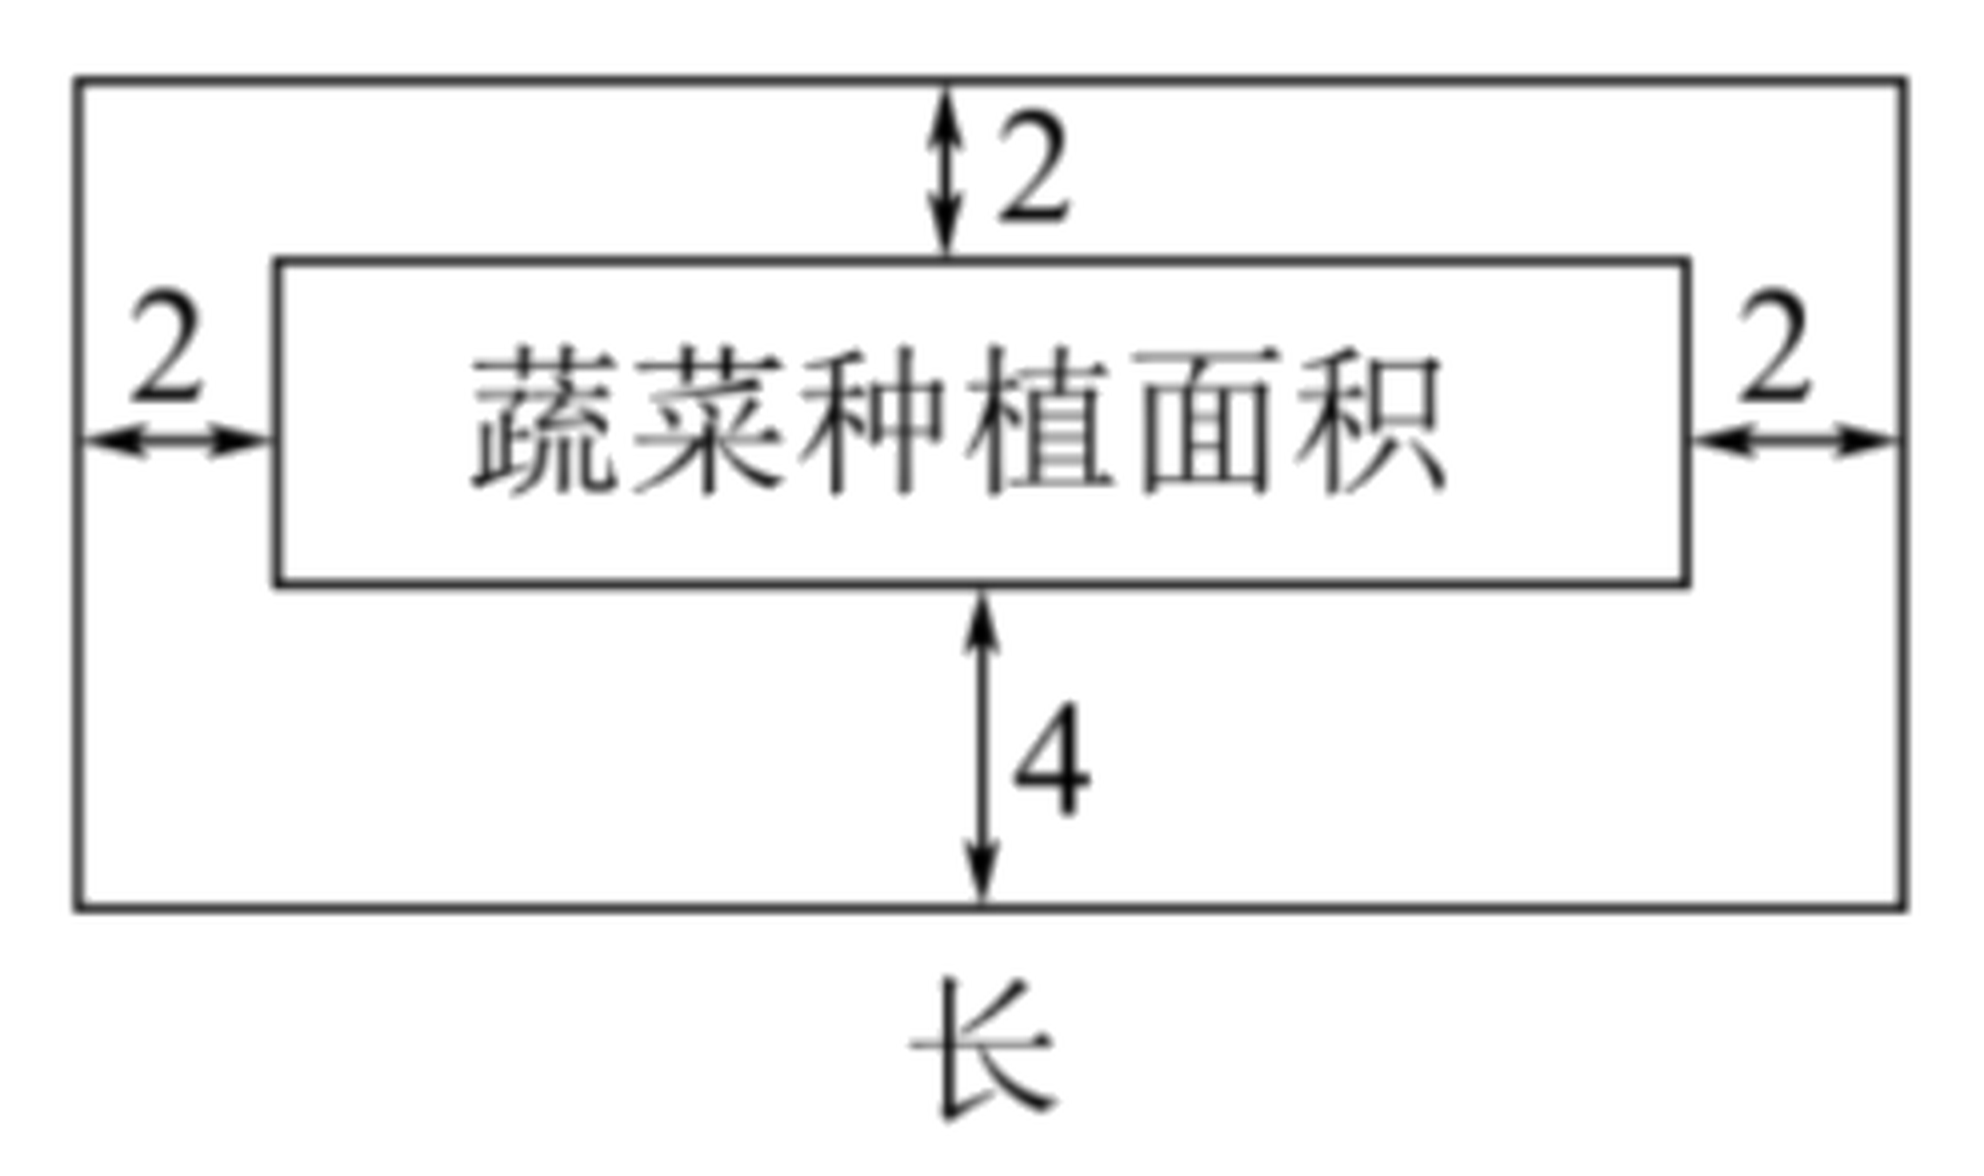
\includegraphics[width=0.45\textwidth]{figures/gao148_q20.png}
\end{center}

(1) 写出蔬菜的种植面积关于矩形温室的长之间的关系式.

(2) 当矩形温室的边长各为多少时，蔬菜的种植面积最大？最大种植面积是多少？

\ifanswer
\solbegin
\step{(1) 设蔬菜的种植面积为 $y\mathrm{m}^2$，矩形温室的长为 $x\mathrm{m}$，}
\step{则矩形温室的宽为 $\dfrac{600}{x}\mathrm{m}$，}
\step{种植蔬菜矩形的长为 $(x-4)\mathrm{m}$，宽为 $\left(\dfrac{600}{x}-6\right)\mathrm{m}$，}
\step{所以 $y=(x-4)\left(\dfrac{600}{x}-6\right)(4<x<100)$；}
\step{(2) 因为 $y=(x-4)\left(\dfrac{600}{x}-6\right)=624-\left(6x+\dfrac{2400}{x}\right)$，}
\step{因为 $6x+\dfrac{2400}{x}\geqslant2\sqrt{6x\cdot\dfrac{2400}{x}}=240$，}
\step{当且仅当 $6x=\dfrac{2400}{x}$，即 $x=20$ 时取等号，}
\step{所以 $y=624-\left(6x+\dfrac{2400}{x}\right)\leqslant624-240=384$.}
\step{即当矩形温室的一边长为 $20\mathrm{m}$，另一边长为 $30\mathrm{m}$ 时，}
\step{蔬菜的种植面积最大，最大为 $384\mathrm{m}^2$.}
\solend
\fi

% === Q21 ===：3 问、cases 块整体算一个印刷行；判别式高 \Delta；解析 19 行（末行续 09 页）
\item 二次函数 $f(x)=ax^2+bx+c$ 满足对任意的 $x\in\R$，$x-1\leqslant f(x)\leqslant x^2-x$ 恒成立.

(1) 求证：$f(1)$ 为定值；

(2) 若 $f(0)=-\dfrac{1}{4}$，求二次函数 $f(x)$ 的表达式；

(3) 求 $a+2b+5c$ 的取值范围.

\ifanswer
\solbegin
\step{(1) 对任意的 $x\in\R$，$x-1\leqslant f(x)\leqslant x^2-x$ 恒成立，则 $0\leqslant f(1)\leqslant0$，}
\step{所以 $f(1)=0$，为定值.}
\step{(2) 由(1)得 $a+b+c=f(1)=0$，由 $f(0)=-\dfrac{1}{4}$，得 $c=-\dfrac{1}{4}$，}
\step{则 $b=\dfrac{1}{4}-a$，$f(x)=ax^2+\left(\dfrac{1}{4}-a\right)x-\dfrac{1}{4}$，}
\step{不等式 $x-1\leqslant f(x)$ 可化为 $ax^2+\left(\dfrac{1}{4}-a\right)x-\dfrac{1}{4}\geqslant x-1$，}
\step{即 $ax^2-\left(a+\dfrac{3}{4}\right)x+\dfrac{3}{4}\geqslant0$，}
\step{一元二次不等式 $ax^2-\left(\dfrac{3}{4}+a\right)x+\dfrac{3}{4}\geqslant0$ 恒成立，则 $\begin{cases}a>0\\\Delta=\left(a+\dfrac{3}{4}\right)^2-3a\leqslant0\end{cases}$，}% 判别式原卷印等腰偏高粗三角 $\Delta$，照录（放大 08 页 q21_delta3.png／diag_band_q21.png 确认）
\step{解得 $a=\dfrac{3}{4}$，}
\step{此时 $f(x)=\dfrac{3}{4}x^2-\dfrac{1}{2}x-\dfrac{1}{4}$，$x^2-x-f(x)=\dfrac{1}{4}(x-1)^2\geqslant0$ 恒成立，}
\step{所以 $f(x)=\dfrac{3}{4}x^2-\dfrac{1}{2}x-\dfrac{1}{4}$.}
\step{(3) 由(1)得 $b=-a-c$，$f(x)=ax^2-(a+c)x+c=(ax-c)(x-1)$，}
\step{不等式 $x-1\leqslant f(x)$ 可化为 $(x-1)(ax-c-1)\geqslant0$，}
\step{一元二次不等式 $(x-1)(ax-c-1)\geqslant0$ 恒成立，则 $a>0$，}
\step{且方程 $(x-1)(ax-c-1)=0$ 有相等的实数根，因此 $c=a-1$，$a>0$，}
\step{不等式 $f(x)\leqslant x^2-x\Leftrightarrow(ax-c)(x-1)\leqslant x^2-x\Leftrightarrow(x-1)[(1-a)x+c]\geqslant0$，}
\step{同理 $1-a>0$，且方程 $(x-1)[(1-a)x+c]=0$ 有相等的实数根，}
\step{因此 $c=a-1$，$a<1$，从而 $c=a-1$，$b=1-2a$，$0<a<1$，}
\step{$a+2b+5c=a+2(1-2a)+5(a-1)=2a-3\in(-3,-1)$，}
\step{所以 $a+2b+5c$ 的取值范围是 $(-3,-1)$.}
\solend
\fi

\end{enumerate}

\end{document}
"
% 紧凑版：xelatex "\def\iscompact{1}% 高一148_新川中学_期中.tex
%   —— 高一上数学"2026-2027 年新川中学高一上期中"（试卷版/答案版/紧凑版）
% 试卷版：xelatex 高一148_新川中学_期中.tex
% 答案版：xelatex "\def\isanswer{1}\input{高一148_新川中学_期中.tex}"
% 紧凑版：xelatex "\def\iscompact{1}\input{高一148_新川中学_期中.tex}"
%
% ① 原始材料：微信公众号"魔都数学加油站"文章，连载"27学年高一148"，原文标题
% "27学年高一148——2026-2027年上海市新川中学高一上期中"（2026-11-21 推送）；
% 原文链接：https://mp.weixin.qq.com/s/Alhmwb3sSLQMp_wjzoAVyA 。
% 正文为 9 张 PNG 页（01/03/04/07/08/09 为 2560×3620，02/05/06 为 4762×6735，
% 同一篇各页分辨率混排，逐页按各自分辨率裁图核对，别按预览比例换算裁框）。
% 体例：混合体例讲评版——19 题中 Q4、Q5 只印【答案】、无【解析】；Q13 的答案"C"
% 直接印在题干括号内、无【答案】/【解析】段；其余 16 题印【解析】（逐题核实，见 ② ②）。
% 题目、答案、解析均据原图转录；卷面粉红色水印"魔都数学加油站"及公众号页脚未录入。
% 全卷插图清单（逐页通读 9 页确认）：4 幅题目配图，均三版都出、均非【解析】内配图：
%   · Q12 幂函数曲线族图（03 页右侧：x/y 轴、O、A(1,0)、B(0,1)、M、N 与两族
%     y=x^α／y=x^β 曲线、线段 AB、虚线），题干"（如图）"处，裁 figures/gao148_q12.png；
%   · Q15 四条指数函数曲线图（04 页右侧：①②③④ 四曲线同过 (0,1)、x/y 轴、O、
%     y 轴刻度 1），题干"如图"处，裁 figures/gao148_q15.png；
%   · Q16 关于 y 轴对称的幂函数曲线图（04 页右下：x/y 轴、O、两支上翘曲线），
%     题干"如图所示"处，裁 figures/gao148_q16.png；
%   · Q20 矩形蔬菜温室示意图（07 页右侧：大矩形＋内框"蔬菜种植面积"＋2/2/4
%     通道标注＋"长"），题干处，裁 figures/gao148_q20.png；
%   其余各页逐页确认无其它题目配图、无【解析】内配图、无表格，亦无"题干写如图而
%   源码漏图"一处；Q19 解析行末的虚线"----N 分"为评分档（非图），Q18／Q21 的
%   cases 块为数学块（非图）。4 图均取自原卷截图，去粉色水印、去色、4× LANCZOS 放大。
%
% 卷首标题：原卷印作"2026-2027 年新川中学高一上期中"，年份区间按全稿惯例排 en dash；
% 原卷卷面未印副标题，本稿按同期中卷（高一140／141／143／144／145／146／147）知识模块
% 口径补出"集合与常用逻辑用语、不等式、函数"。
%
% 题号体例（逐页核实定稿）：本卷共 19 题——一、填空题 3—12（10 题）、
% 二、选择题 13—16（4 题）、三、解答题 17—21（5 题）。
% 三节分别 \setcounter{enumi}{2}／{12}／{16}。原卷从第 3 题起、无第 1、2 题，
% 本稿保留原题号；全卷无附加题节、无 Q22（Q21 解析末行"所以 a+2b+5c 的取值范围是
% (-3,-1)."为全卷收尾，09 页下半仅水印、无正文）。
%
% ② 与原卷的排版差异：
%   ① 原文从第 3 题起，本稿保留原题号；共 19 题三节；
%   ② 混合体例逐题核实：Q4（反证法"假设的内容"）、Q5 只印【答案】、无【解析】，
%      按 高一140 第 5 题／高一145 Q3 成例提 \ans{}、不补造解析；Q13 答案"C"直接
%      印在题干括号内（" ( C ) "）、全卷无该题【答案】/【解析】段，按 高一84 Q13／
%      高一37 Q13／高一53 Q13 成例括号 \mbox{（\quad）} 留空、另提 \ans{$C$}；
%      其余 16 题印【解析】、用 \solbegin…\solend，选择题答案在解析末句"故选 X"
%      （Q14 选 D、Q15 选 B、Q16 选 D，逐个放大原图核实）、题干括号留空、不另提
%      \ans{}；答案版【答案】/【解析】标记数 = 19（3 个 \ans ＋ 16 个 \solbegin）
%      = 全卷题数；
%   ③ 原卷卷面未印副标题，本稿按知识模块口径补出；
%   ④ 原卷填空横线按全稿惯例排 \blankline[4.4em]；选择题括号排 \mbox{（\quad）}、
%      选项段前按惯例加 \keepwithprev；Q13／Q16 四选项为两行两列、Q14／Q15 选项
%      为一行，照原卷分行；解答题不留作答区、不加 \anspace（原卷为讲评版，
%      与 129／131／132／133／136／140／141／143／144／145／146 同）；
%   ⑤ 数集：Q11"在 R 上定义运算"、Q13"x、y∈R"、Q16"p、q∈Z"、Q17"a∈R"
%      "U=R"、Q19"m∈R"、Q21"x∈R" 原卷印斜体 R/Z，按全稿惯例统一改 \R／\Z
%      （本卷未出现 N，\N^* 无对应处）；绝对值排 \lvert…\rvert（Q9／Q14），
%      集合描述竖线排 \mid（Q17）；不等号按全稿惯例排 \leqslant／\geqslant；
%      补集照原卷上划线排 \overline{B}（Q17 题干 1 处＋解析 3 处）；空集
%      \varnothing（Q17 题干 1 处＋解析 2 处）；\subset（Q3 题干 {a}⊂M）与
%      \subseteq（Q3 题干 M⊆{a,b,c,d}）逐处照录不统一（放大 01 页 q3_subset.png）；
%   ⑥ 子题标号 (1)(2)(3) 半角括号照录；圈数字 ①—⑥ 在文本模式（Q14 六个结论、
%      Q15 曲线编号与其解析、Q14 解析"对①…对⑥"），按 common.sty 划入 CJK 字符类
%      渲染；cases 块整体算一个印刷行；\left…\right 不得拆到不同 $…$ 组；
%      单位 m／m² 排 \mathrm{m}／\mathrm{m}^2（Q20，原卷印正体 m）；
%   ⑦ 题干／解析中的中文弯引号按原卷照录：Q4" ab 可以被 5 整除，那么 a、b 中
%      至少有一个能被 5 整除 "（开引号后有空格、闭引号后空格接"时"）、
%      Q13" x=0 "" xy=0 "（引号内空格），注释内一律 ASCII 引号；
%   ⑧ 半角逗号在数学组之间是全稿惯例、非笔误（Q3"{a,b,c,d}"、Q6"$x,y$"
%      "$x=\frac13,y=\frac16$"、Q10、Q11"$a=-2,b=-1"、Q12"$\alpha=\log..,\beta=..$"、
%      Q14"$a+b<0,a-b<0$"、Q17、Q19"$x_1+x_2=-6,x_1\cdot x_2=7$"、Q20、Q21 等），
%      逐处照录别改全角；行末西文句点照录为 ASCII `.`；行中全角逗号／顿号照录；
%   ⑨ "图像／图象"逐处放大核：全卷 9 处均印"图象"（象，无亻）、未见"图像"，
%      逐处照录未统一改动（Q8 题干/解析各 1、Q12 题干 2、Q15 题干 1／解析 2、
%      Q16 题干 1／解析 1；放大 02/03/04/05 页 /tmp/gao148/zoom/my_wide_a.png、
%      my_wide_b.png 与宋体参考"象／像"并排确认）；
%   ⑩ 判别式 Δ/△ 混用是照录项：Q11 解析"△=1−4(−a²+a+1)<0"印扁等边空心
%      三角 \triangle；Q19 解析"Δ=36m²−4(9m−2)>0"、Q21 解析 cases 块
%      "Δ=(a+3/4)²−3a≤0" 两处印等腰偏高粗三角 \Delta，逐处放大判断、照录
%      不统一（参照 高一142／144／145 头注④口径，详见 ④）；
%   ⑪ 一条 \step = 原卷解析的一个印刷行，cases 块整体算一个印刷行；别把原卷折行
%      并起来、别把一行拆多条。Q3 六行、Q7 五行（01 页末首行＋02 页顶四行）、
%      Q9 七行、Q11 五行、Q14 八行（对② 的两行公式各占一印刷行）、Q17 八行、
%      Q18 六行、Q19 九行（7 处评分档附在行末）、Q20 十行、Q21 十九行
%      均按印刷行逐条断，不丢行；
%   ⑫ 配图：4 幅均为题目配图（三版都出），放 \item 内题干之后 \begin{center}；
%      大图块加 \needvspace 守卫把整块推走（守卫放 \item 之前，见 高一145 Q14/Q20
%      成例与切页审计 B 类坑）；三版切页审计均"合计异常：无"；
%   ⑬ 跨页续印按题合并：Q3/4/5 在 01 页；Q6 题干＋解析在 01 页；Q7 题干在 01 页
%      末、解析首行在 01 页末续 02 页顶四行；Q8/9/10 在 02 页（Q9 解析续 02 页下半、
%      Q10 题干与解析前 2 行在 02 页末）；Q10 解析末行续 03 页顶；Q11/12 在 03 页、
%      "二、选择题"标题与 Q13/14 题干在 03 页下半；Q13 无解析；Q14 解析在 04 页顶、
%      Q15 题干＋图＋选项＋解析在 04 页、Q16 题干＋图在 04 页末；Q16 选项＋解析＋
%      "三、解答题"标题＋Q17 题干＋解析在 05 页、Q18 题干首句在 05 页末；Q18 题干
%      续＋解析、Q19 题干＋解析前 5 行在 06 页；Q19 解析续 4 行＋Q20 题干＋图＋
%      解析（10 行全部）在 07 页，末行"蔬菜的种植面积最大，最大为 384m²."收尾；
%      Q21 题干＋解析前 18 行在 08 页；Q21 解析末行"所以 a+2b+5c 的取值范围是
%      (-3,-1)."在 09 页上半（09 页下半仅水印、无正文）。本稿按题连排，不丢行、
%      不并折行；
%   ⑭ 原卷解析内无红色"法一／法二"之类小标题，故本卷无 \stepm；水印
%      "魔都数学加油站"红色不录入；Q19 解析 7 处评分档（1/2/3/2/2/2/2 分）
%      原卷在行末印一串虚线，本稿照 高一54／64 成例排 \dots\dots N 分，
%      分值逐处照录、位置不变。
%
% ③ 行数复核：一条 \step／\stepm = 原卷解析的一个印刷行，cases 块作一个印刷行计。
%   逐题数（主会话逐页核对定稿）：Q3：6；Q4：0（只印【答案】、提 \ans{}）；
%   Q5：0（只印【答案】、提 \ans{}）；Q6：2；Q7：5；Q8：2；Q9：7；Q10：3；
%   Q11：5；Q12：2；Q13：0（答案印在题干括号内、另提 \ans{}）；Q14：8；Q15：5；
%   Q16：2；Q17：8；Q18：6；Q19：9；Q20：10；Q21：19。
%   合计 99 条 \step（本卷无 \stepm：解析内无红色"法一／法二"类小标题），
%   与原卷逐题印刷行相等。全卷 16 题设 \solbegin…\solend ＋ 3 处 \ans{}，
%   答案版【答案】/【解析】标记数 = 19 = 全卷题数。
%
% ④ 判别式／子集符号结论（逐处放大原图照录、不得统一，主会话像素级复核）：
%   判别式全卷 3 处，两形混用逐处照录不统一（参照 高一142／144／145 头注④口径）：
%     · Q11 解析"△=1−4(−a²+a+1)<0" 原卷印扁等边空心三角（宽>高、细线），
%       照录 \triangle（放大 03 页 /tmp/gao148/zoom/q11_delta3.png、
%       delta_montage.png 确认）；
%     · Q19 解析"Δ=36m²−4(9m−2)>0" 原卷印等腰偏高粗三角（高>宽），
%       照录 \Delta（放大 07 页 /tmp/gao148/zoom/q19_delta3.png 确认）；
%     · Q21 解析 cases 块"Δ=(a+3/4)²−3a≤0" 原卷印等腰偏高粗三角（高>宽），
%       照录 \Delta（放大 08 页 /tmp/gao148/zoom/q21_delta3.png 确认）。
%   子集／补集：Q3 题干"{a}⊂M⊆{a,b,c,d}" 前者印单线 ⊂、无下划线，照录 \subset；
%     后者印带下划线 ⊆，照录 \subseteq（放大 01 页 /tmp/gao148/zoom/q3_subset.png
%     确认）；Q17 题干 1 处＋解析 3 处共 4 处 \overline{B} 照原卷上划线
%     （B 上横线、非 C_U B）；空集 \varnothing 3 处（Q17 题干 1 处、解析 2 处）；
%     Q17 集合描述竖线 \mid；数集 \R／\Z 归一见 ② ⑤。
%
% ⑤ 存疑照录（放大原图确认，照录未改、正文对应处另有 % 注）：
%   1. Q3 解析末行"所以 M 一共有 3+3+1+1=8 个" 原卷印 $3+3+1+1=8$，按上文
%      四行应为 $1+3+3+1=8$（疑为原卷加数顺序笔误，和仍为 8），放大 01 页
%      /tmp/gao148/zoom/my_q3_sol.png 确认，照录未改。
%   2. Q13 答案"C"直接印在题干括号内、全卷无该题【答案】/【解析】段，按
%      高一84 Q13 成例括号留空、另提 \ans{$C$}（见 ② ②），未补造解析。
%   3. Q19 解析 7 处评分档（"----N 分"）原卷印一串虚线，本稿照 高一54／64
%      成例排 \dots\dots N 分，分值逐处照录、位置不变。
%   4. 判别式 Q11 扁 \triangle 与 Q19／Q21 高 \Delta 两形混用，逐处照录不统一（见 ④）。
%   5. "图像／图象"全卷 9 处均印"图象"、未见"图像"（见 ② ⑨），逐处放大核实照录，
%      未统一改动。
%   全卷除此 5 类外未发现其它笔误／自相矛盾处。
%
% ⑥ 跨页续印按题合并说明：见 ② ⑬。
%
\documentclass[a4paper,11pt]{article}
\usepackage{common}

\begin{document}

\examtitlest[3]{2026--2027 年新川中学高一上期中}{集合与常用逻辑用语、不等式、函数}

\bigsec{一、填空题}

\begin{enumerate}
\setcounter{enumi}{2}

% === Q3 ===：题干 {a}⊂M⊆{a,b,c,d} 两个子集符号逐处照录；解析 6 行
\item 满足 $\{a\}\subset M\subseteq\{a,b,c,d\}$ 的集合 $M$ 有\blankline[4.4em]个.

\ifanswer
\solbegin
\step{$M$ 是 $\{a,b,c,d\}$ 的子集，但必含有元素 $a$，}
\step{当 $M$ 中只一个元素时，$M=\{a\}$ 只有 1 个；}
\step{当 $M$ 中有二个元素时，$M$ 有 3 个；}
\step{当 $M$ 中有三个元素时，$M$ 有 3 个；}
\step{当 $M$ 中有四个元素时，$M$ 有 1 个；}
\step{所以 $M$ 一共有 $3+3+1+1=8$ 个.}% 原卷印 $3+3+1+1=8$（按上文四行应为 $1+3+3+1$），疑为加数顺序笔误，照录未改（放大 01 页 my_q3_sol.png）
\solend
\fi

% === Q4 ===：原卷只印【答案】、无【解析】，按 高一140 第 5 题成例提 \ans{}；弯引号与空格照录
\item 用反证法证明命题 “ $ab$ 可以被 5 整除，那么 $a$、$b$ 中至少有一个能被 5 整除” 时假设的内容应该是\blankline[4.4em].

\ifanswer
\ans{$a$、$b$ 都不能被 5 整除}
\fi

% === Q5 ===：原卷只印【答案】 $[-2,1)$、无【解析】，提 \ans{}
\item 不等式 $\dfrac{x+2}{x-1}\leqslant0$ 的解集为\blankline[4.4em].

\ifanswer
\ans{$[-2,1)$}
\fi

% === Q6 ===：解析 2 行；半角逗号在数学组之间照录
\item 设 $x,y\in(0,+\infty)$，且 $x+4y=1$，则 $\dfrac{1}{x}+\dfrac{1}{y}$ 的最小值为\blankline[4.4em].

\ifanswer
\solbegin
\step{因为 $\dfrac{1}{x}+\dfrac{1}{y}=(x+4y)\left(\dfrac{1}{x}+\dfrac{1}{y}\right)=5+\dfrac{4y}{x}+\dfrac{x}{y}\geqslant5+2\sqrt{\dfrac{4y}{x}\cdot\dfrac{x}{y}}=9$，}
\step{当且仅当 $\dfrac{4y}{x}=\dfrac{x}{y}$，即 $x=2y$，即 $x=\dfrac{1}{3},y=\dfrac{1}{6}$ 时取等号，故最小值为 9.}
\solend
\fi

% === Q7 ===：题干在 01 页末、解析首行在 01 页末续 02 页顶四行；解析 5 行
\item 若不等式 $x^2+ax+b<0$ 的解集为 $(-3,-1)$，则不等式 $bx^2+ax+1\leqslant0$ 的解集为\blankline[4.4em].

\ifanswer
\solbegin
\step{不等式 $x^2+ax+b<0$ 的解集为 $(-3,-1)$，}
\step{所以方程 $x^2+ax+b=0$ 的两个实数根为 $-3$ 和 $-1$，}
\step{由根与系数的关系得 $a=4$，$b=3$，}
\step{故 $bx^2+ax+1\leqslant0$ 可化为 $3x^2+4x+1\leqslant0$，解得 $-1\leqslant x\leqslant-\dfrac{1}{3}$，}
\step{所求不等式 $bx^2+ax+1\leqslant0$ 的解集为 $\left[-1,-\dfrac{1}{3}\right]$.}
\solend
\fi

% === Q8 ===："图象"照录；解析 2 行
\item 函数 $y=a^{x-2}+2(a>0,a\ne1)$ 的图象必经过定点\blankline[4.4em].

\ifanswer
\solbegin
\step{令 $x-2=0$，得 $x=2$，则 $y=a^0+2=3$，}
\step{所以函数 $y=a^{x-2}+2$ 的图象过定点 $(2,3)$.}
\solend
\fi

% === Q9 ===：解析 7 行；首句末西文句点照录
\item 不等式 $\lvert x+3\rvert+\lvert a-x\rvert>6$ 对一切实数 $x$ 恒成立，则实数 $a$ 的取值范围为\blankline[4.4em].

\ifanswer
\solbegin
\step{$\lvert x+3\rvert$ 表示 $x$ 到 $-3$ 的距离，$\lvert a-x\rvert$ 表示 $x$ 到 $a$ 的距离.}
\step{所以它们的和为 $x$ 到 $-3$ 和 $x$ 到 $a$ 的距离之和，}
\step{当 $x$ 位于 $-3$ 和 $a$ 之间时，距离和取得最小值，}
\step{即两点之间的距离 $\lvert a-(-3)\rvert=\lvert a+3\rvert$，}
\step{若最小值 $\lvert a+3\rvert>6$，则原式对所有 $x$ 恒成立.}
\step{解得 $a+3>6$ 或 $a+3<-6$，即 $a>3$ 或 $a<-9$，}
\step{故 $a\in(3,+\infty)$ 或 $a\in(-\infty,-9)$.}
\solend
\fi

% === Q10 ===：题干与解析前 2 行在 02 页末、解析末行续 03 页顶；解析 3 行
\item 已知 $2^a=3$，$\log_3 5=b$，则 $\log_{15}20=$\blankline[4.4em]（用 $a$、$b$ 表示）.

\ifanswer
\solbegin
\step{因为 $2^a=3$，所以 $a=\log_2 3=\dfrac{\lg3}{\lg2}$，又 $\log_3 5=b=\dfrac{\lg5}{\lg3}$，}
\step{所以 $\lg3=a\lg2$，$\lg5=b\lg3=ba\lg2$，}
\step{则 $\log_{15}20=\dfrac{2\lg2+\lg5}{\lg3+\lg5}=\dfrac{2\lg2+ab\lg2}{a\lg2+ab\lg2}=\dfrac{2+ab}{a+ab}$.}
\solend
\fi

% === Q11 ===：在 \R 上定义运算 \otimes；判别式扁 \triangle 照录；解析 5 行
\item 在 $\R$ 上定义运算 $\otimes:x\otimes y=x(1-y)$，若不等式 $(x-a)\otimes(x+a)<1$ 对任意实数 $x$ 恒成立，则 $a$ 的取值范围是\blankline[4.4em].

\ifanswer
\solbegin
\step{由题意得不等式 $(x-a)\otimes(x+a)<1$ 对任意实数 $x$ 恒成立，}
\step{即不等式 $(x-a)(1-x-a)<1$ 对任意实数 $x$ 恒成立，}
\step{即 $x^2-x-a^2+a+1>0$ 对任意实数 $x$ 恒成立，}
\step{所以 $\triangle=1-4(-a^2+a+1)<0$，解得 $-\dfrac{1}{2}<a<\dfrac{3}{2}$，}% 判别式原卷印扁等边空心三角 $\triangle$，照录（放大 03 页 q11_delta3.png 确认）
\step{所以实数 $a$ 的取值范围为 $\left(-\dfrac{1}{2},\dfrac{3}{2}\right)$.}
\solend
\fi

% === Q12 ===：题目配图（幂函数曲线族，三版都出）；"图象"照录；解析 2 行
\needvspace{8cm}
\item 幂函数 $y=x^\alpha$，当 $\alpha$ 取不同的正数时，在区间 $[0,1]$ 上它们的图象是一族美丽的曲线（如图）. 设点 $A(1,0)$，$B(0,1)$，连接 $AB$，线段 $AB$ 恰好被其中的两个幂函数 $y=x^\alpha$，$y=x^\beta$ 的图象三等分，即有 $BM=MN=NA$，那么 $\alpha\beta=$\blankline[4.4em].

\begin{center}
% 幂函数曲线族图取 03 页右侧，去粉色水印、去色、4× LANCZOS 放大；三版都出
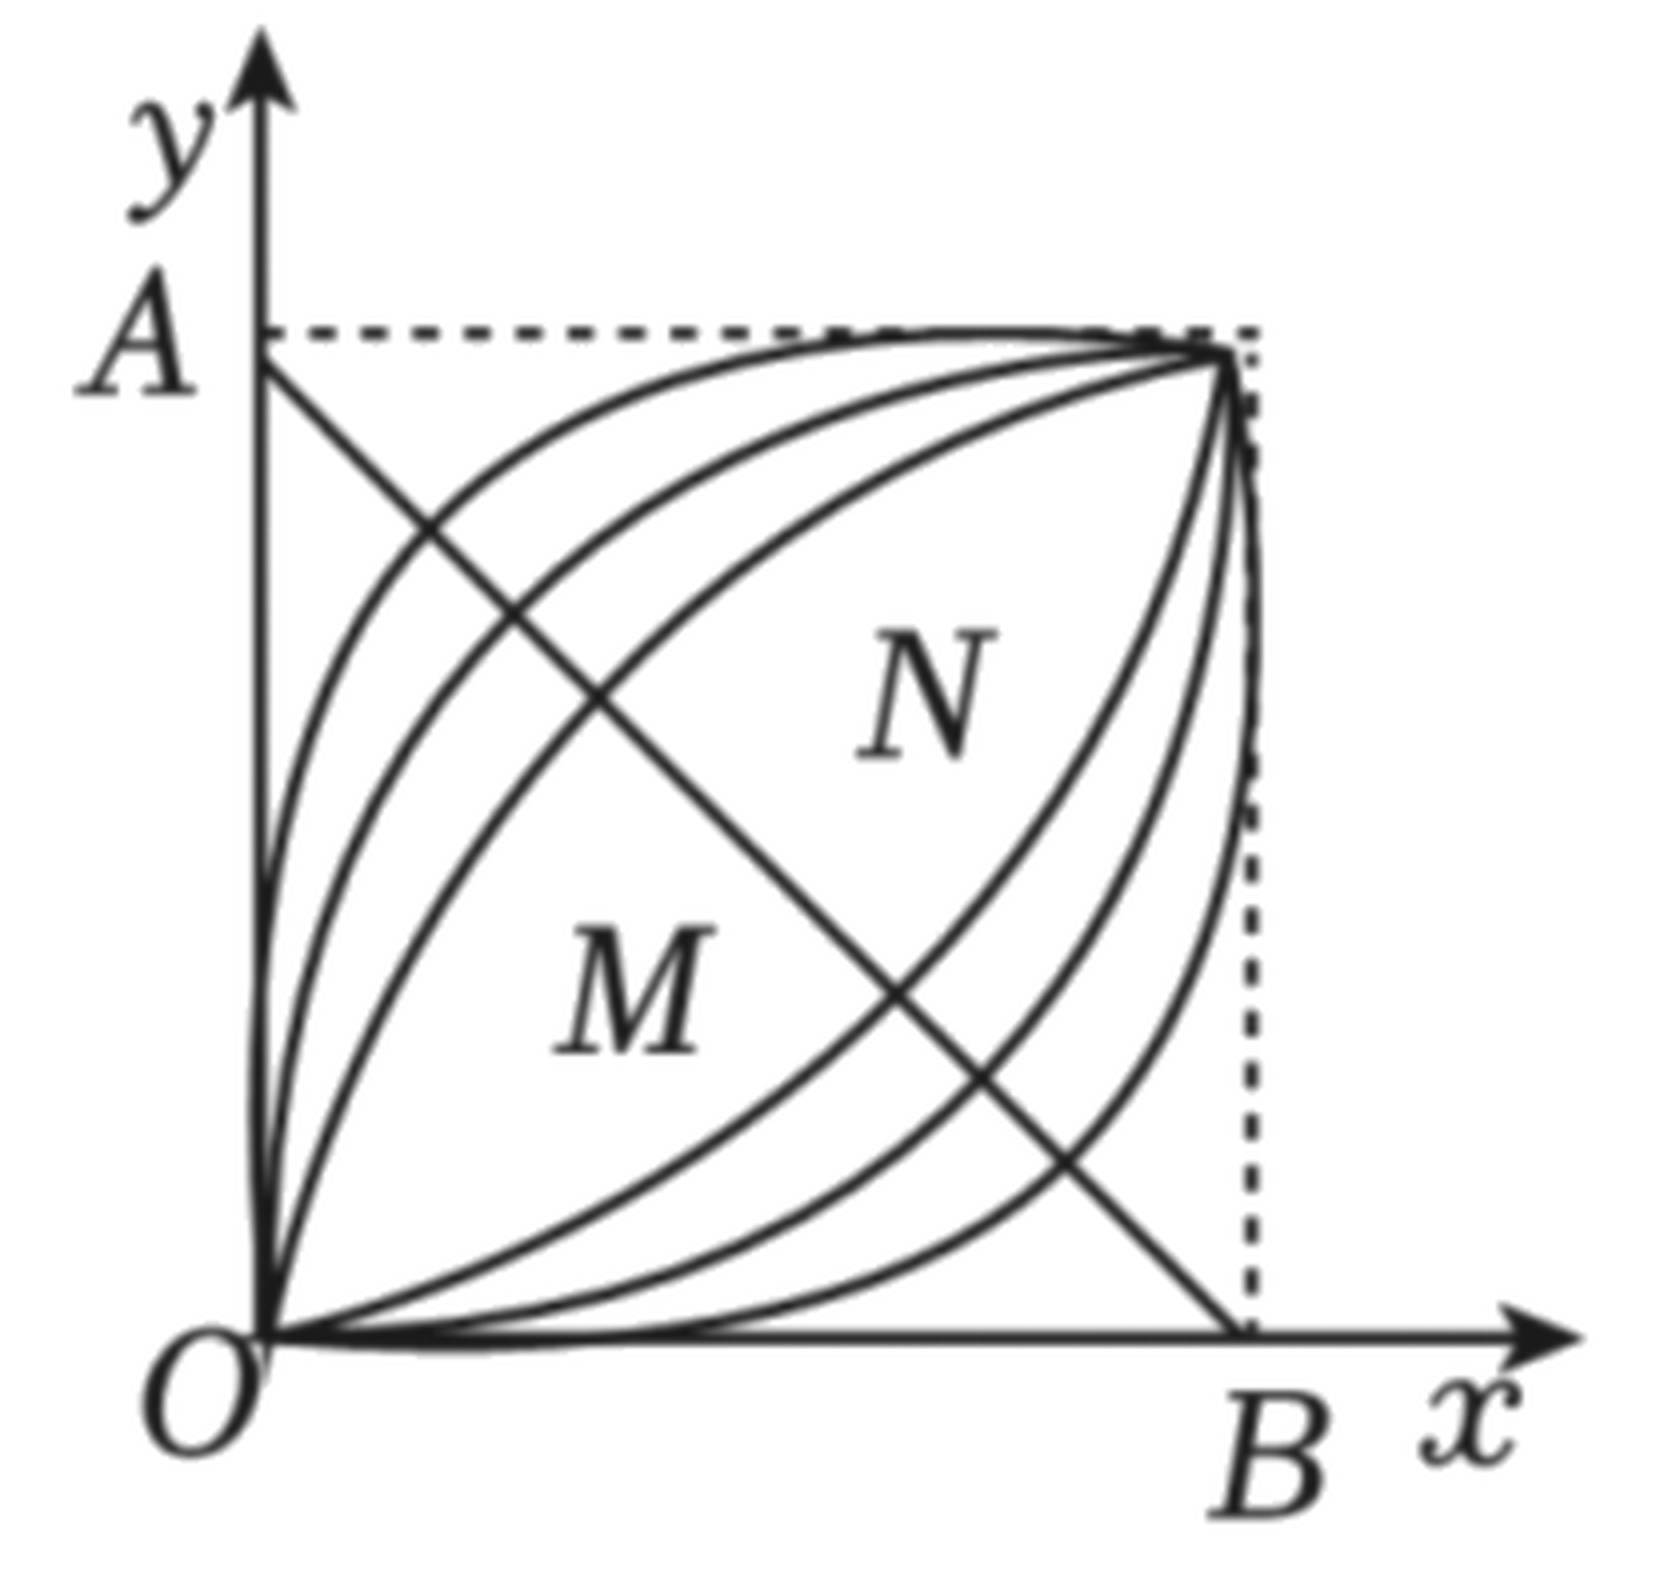
\includegraphics[width=0.40\textwidth]{figures/gao148_q12.png}
\end{center}

\ifanswer
\solbegin
\step{$BM=MN=NA$，点 $A(1,0)$，$B(0,1)$，所以 $M\left(\dfrac{1}{3},\dfrac{2}{3}\right)$，$N\left(\dfrac{2}{3},\dfrac{1}{3}\right)$，}
\step{分别代入 $y=x^\alpha$，$y=x^\beta$，$\alpha=\log_{\frac{2}{3}}\dfrac{1}{3},\beta=\log_{\frac{1}{3}}\dfrac{2}{3}$，$\alpha\beta=\log_{\frac{1}{3}}\dfrac{2}{3}\cdot\log_{\frac{2}{3}}\dfrac{1}{3}=1$.}
\solend
\fi

\end{enumerate}

\bigsec{二、选择题}

\begin{enumerate}
\setcounter{enumi}{12}

% === Q13 ===：答案"C"直接印在题干括号内、全卷无该题【答案】/【解析】段，按 高一84 Q13 成例括号留空、另提 \ans{$C$}；弯引号含空格
\item 若 $x$、$y\in\R$，则 “ $x=0$ ” 是 “ $xy=0$ ” 的\mbox{（\quad）}

\keepwithprev
A. 充要条件\qquad\qquad B. 必要不充分条件

C. 充分不必要条件\qquad\qquad D. 既不充分也不必要条件

\ifanswer
\ans{$C$}
\fi

% === Q14 ===：六个结论（圈数字在文本模式）、四选项一行；解析 8 行（对② 的两行公式各占一印刷行）
\item 若 $a<b<0$，下面有六个结论：① $a^2>b^2$；② $a^3<b^3$；③ $\dfrac{1}{a}<\dfrac{1}{b}$；④ $\dfrac{a}{b}>1$；⑤ $\dfrac{1}{a-b}>\dfrac{1}{a}$；⑥ $\lvert a\rvert>-b$. 其中正确的个数是\mbox{（\quad）}

\keepwithprev
A. 1\qquad\qquad B. 2\qquad\qquad C. 3\qquad\qquad D. 4

\ifanswer
\solbegin
\step{对①：$a^2-b^2=(a+b)(a-b),a+b<0,a-b<0$，故 $a^2-b^2>0$，正确；}
\step{对②：$a^3-b^3=(a-b)(a^2+ab+b^2)=(a-b)\left[\left(a+\dfrac{1}{2}b\right)^2+\dfrac{3}{4}b^2\right],a-b<0$，}
\step{$\left(a+\dfrac{1}{2}b\right)^2+\dfrac{3}{4}b^2>0$，故 $a^3-b^3<0$，正确；}
\step{对③：取 $a=-2,b=-1$，则 $\dfrac{1}{a}=-\dfrac{1}{2},\dfrac{1}{b}=-1,\dfrac{1}{a}>\dfrac{1}{b}$，错误；}
\step{对④：$\dfrac{a}{b}-1=\dfrac{a-b}{b},a-b<0,b<0$，故 $\dfrac{a}{b}-1>0$，正确；}
\step{对⑤：取 $a=-2,b=-1$，则 $\dfrac{1}{a-b}=-1,\dfrac{1}{a}=-\dfrac{1}{2},\dfrac{1}{a-b}<\dfrac{1}{a}$，错误；}
\step{对⑥：要证 $\lvert a\rvert>-b$，即 $-a>-b$，即 $a<b$，正确；}
\step{故选 $D$.}
\solend
\fi

% === Q15 ===：题目配图（四条指数函数曲线，三版都出），\needvspace 守卫放 \item 之前；"图象"照录；解析 5 行
\needvspace{8cm}
\item 如图，曲线①②③④分别是指数函数 $y=a^x$，$y=b^x$，$y=c^x$，$y=d^x$ 的图象，则实数 $a$、$b$、$c$、$d$ 的大小关系为\mbox{（\quad）}

\keepwithprev
A. $a<b<c<d$\qquad B. $b<a<d<c$\qquad C. $d<c<b<a$\qquad D. $c<d<a<b$

\begin{center}
% 四条指数函数曲线图取 04 页右侧，去粉色水印、去色、4× LANCZOS 放大；三版都出
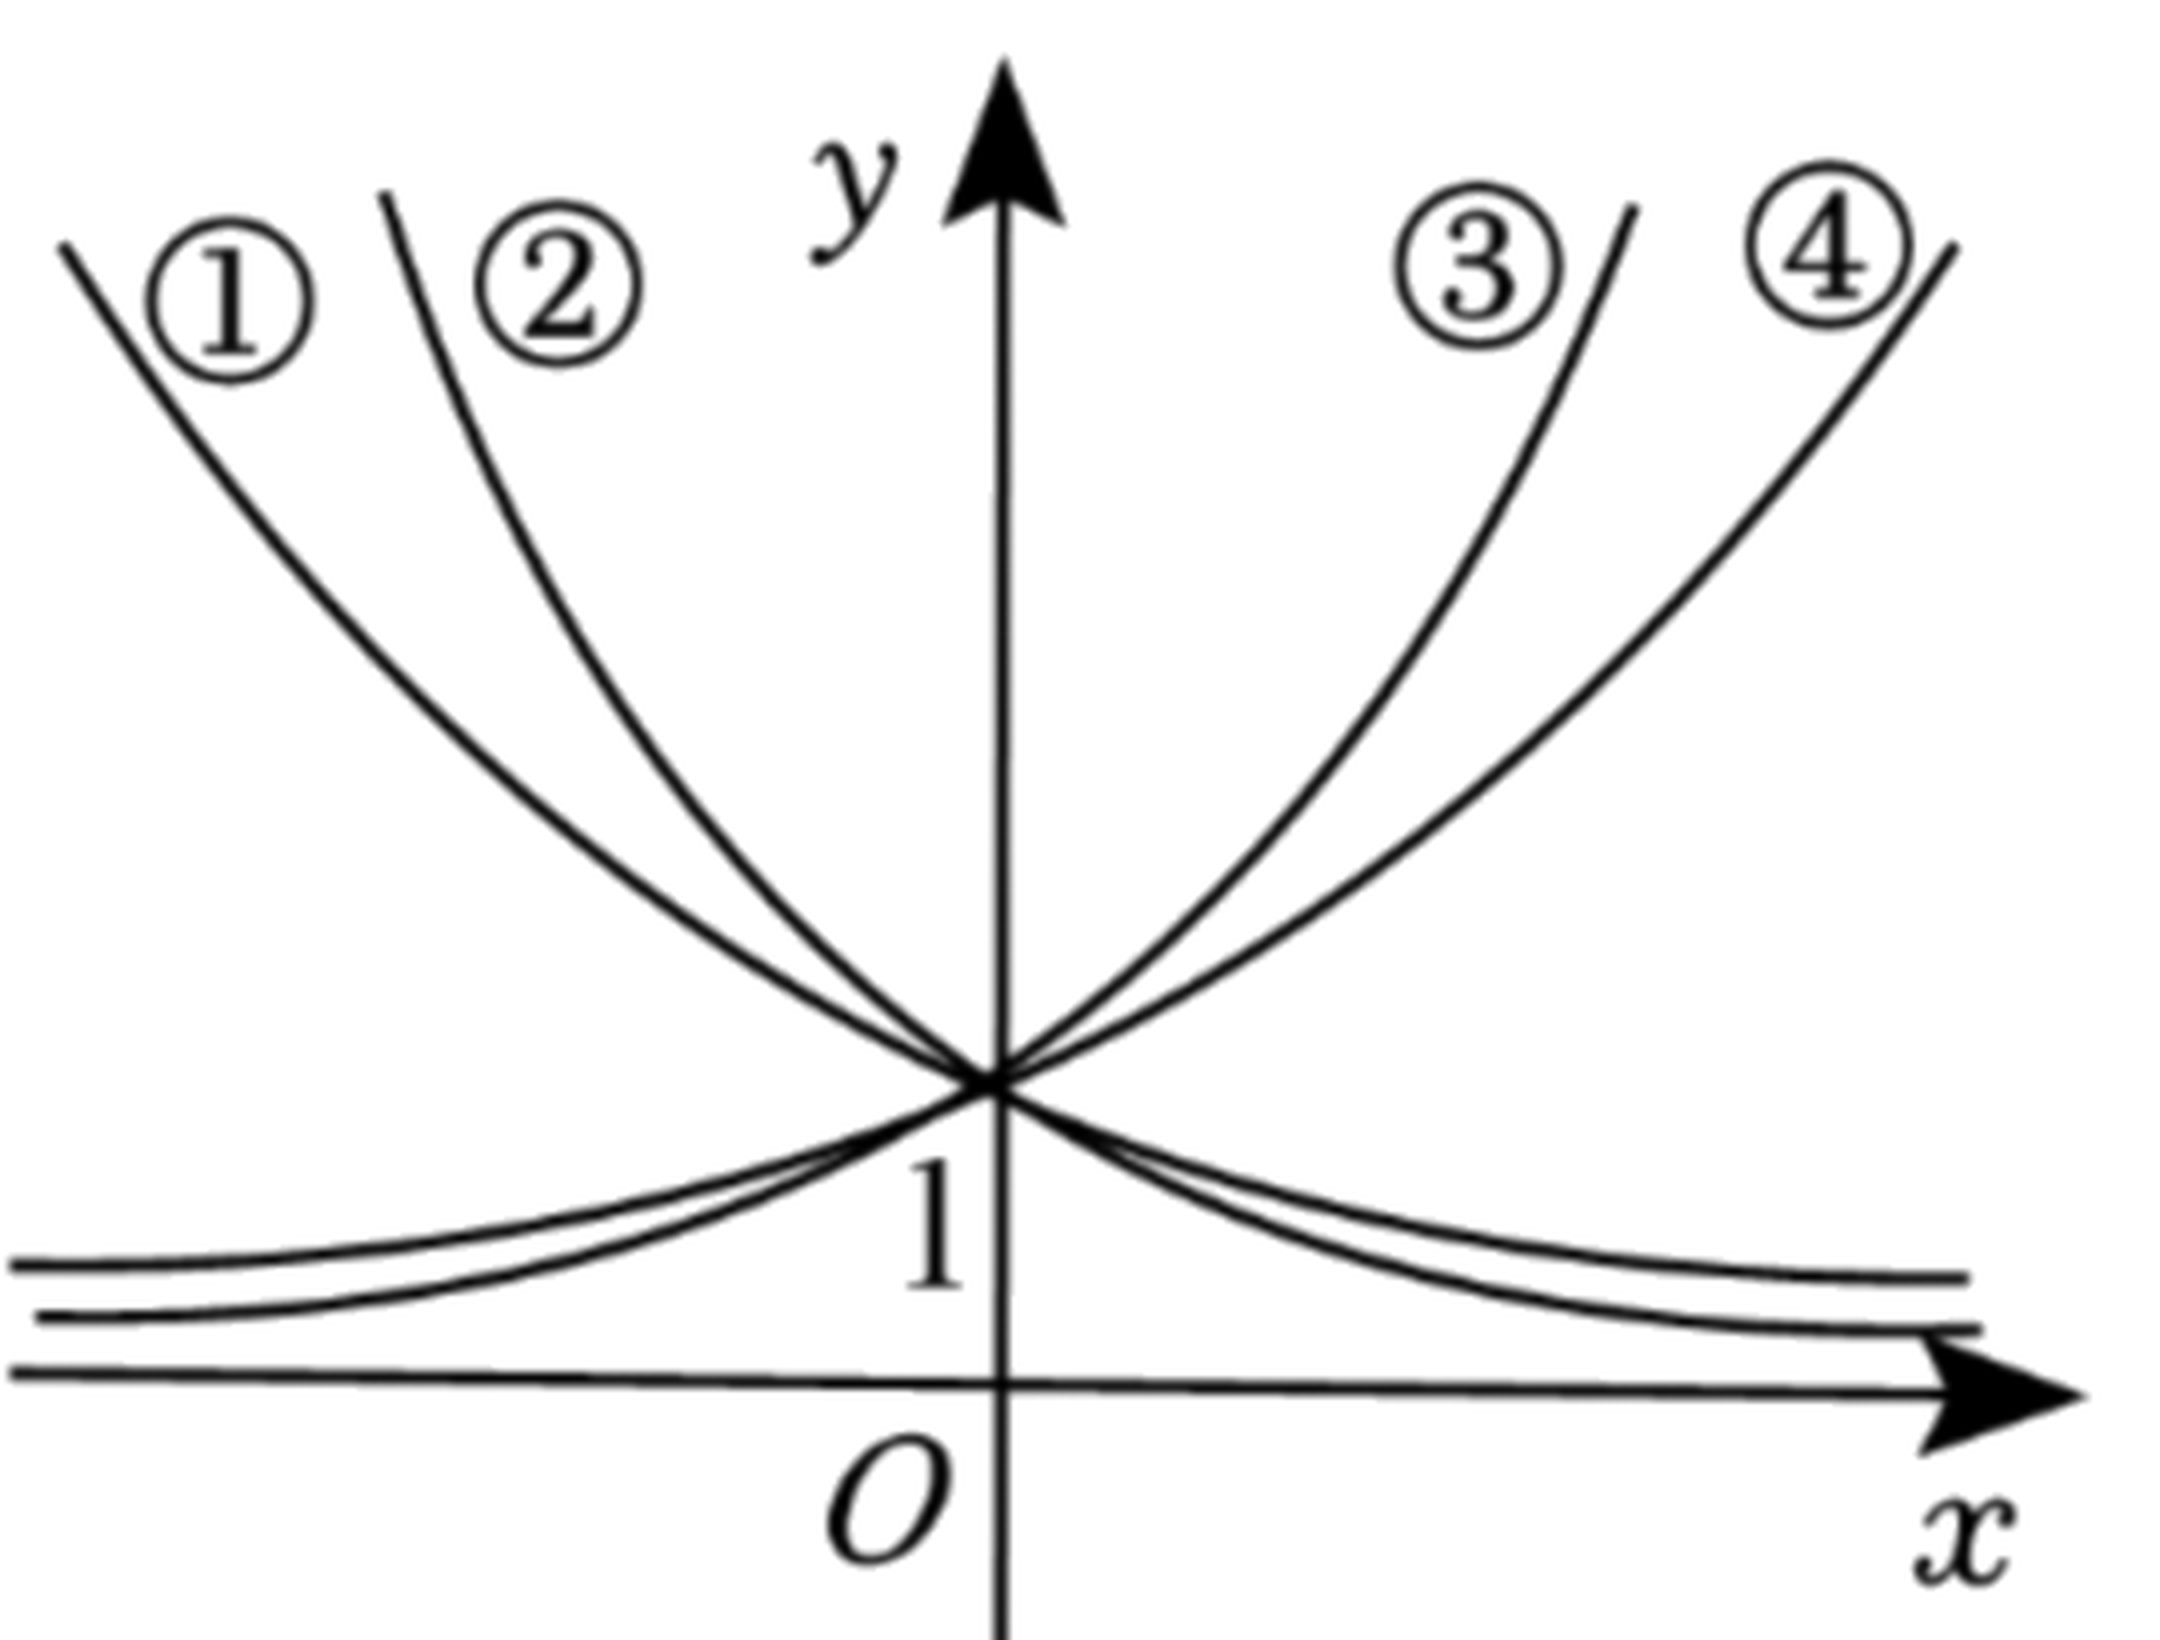
\includegraphics[width=0.40\textwidth]{figures/gao148_q15.png}
\end{center}

\ifanswer
\solbegin
\step{由函数图象得函数① $y=a^x$；② $y=b^x$ 为减函数，且 $x=1$ 时，$b^1<a^1$，}
\step{所以 $0<b<a<1$，}
\step{由函数图象得函数③ $y=c^x$；④ $y=d^x$ 为增函数，且 $x=1$ 时，$c^1>d^1$，}
\step{所以 $c>d>1$，}
\step{所以 $b<a<d<c$. 故选 $B$.}
\solend
\fi

% === Q16 ===：题目配图（关于 y 轴对称的幂函数曲线，三版都出），\needvspace 守卫放 \item 之前；$p$、$q\in\Z$；"图象"照录；解析 2 行
\needvspace{8cm}
\item 已知幂函数 $y=x^{\frac{p}{q}}$（$p$、$q\in\Z$ 且 $p$、$q$ 互质）的图象关于 $y$ 轴对称，如图所示，则\mbox{（\quad）}

\keepwithprev
A. $p$、$q$ 均为奇数，且 $\dfrac{p}{q}>0$\qquad\qquad B. $q$ 为偶数，$p$ 为奇数，且 $\dfrac{p}{q}<0$

C. $q$ 为奇数，$p$ 为偶数，且 $\dfrac{p}{q}>0$\qquad\qquad D. $q$ 为奇数，$p$ 为偶数，且 $\dfrac{p}{q}<0$

\begin{center}
% 关于 y 轴对称的幂函数曲线图取 04 页右下，去粉色水印、去色、4× LANCZOS 放大；三版都出
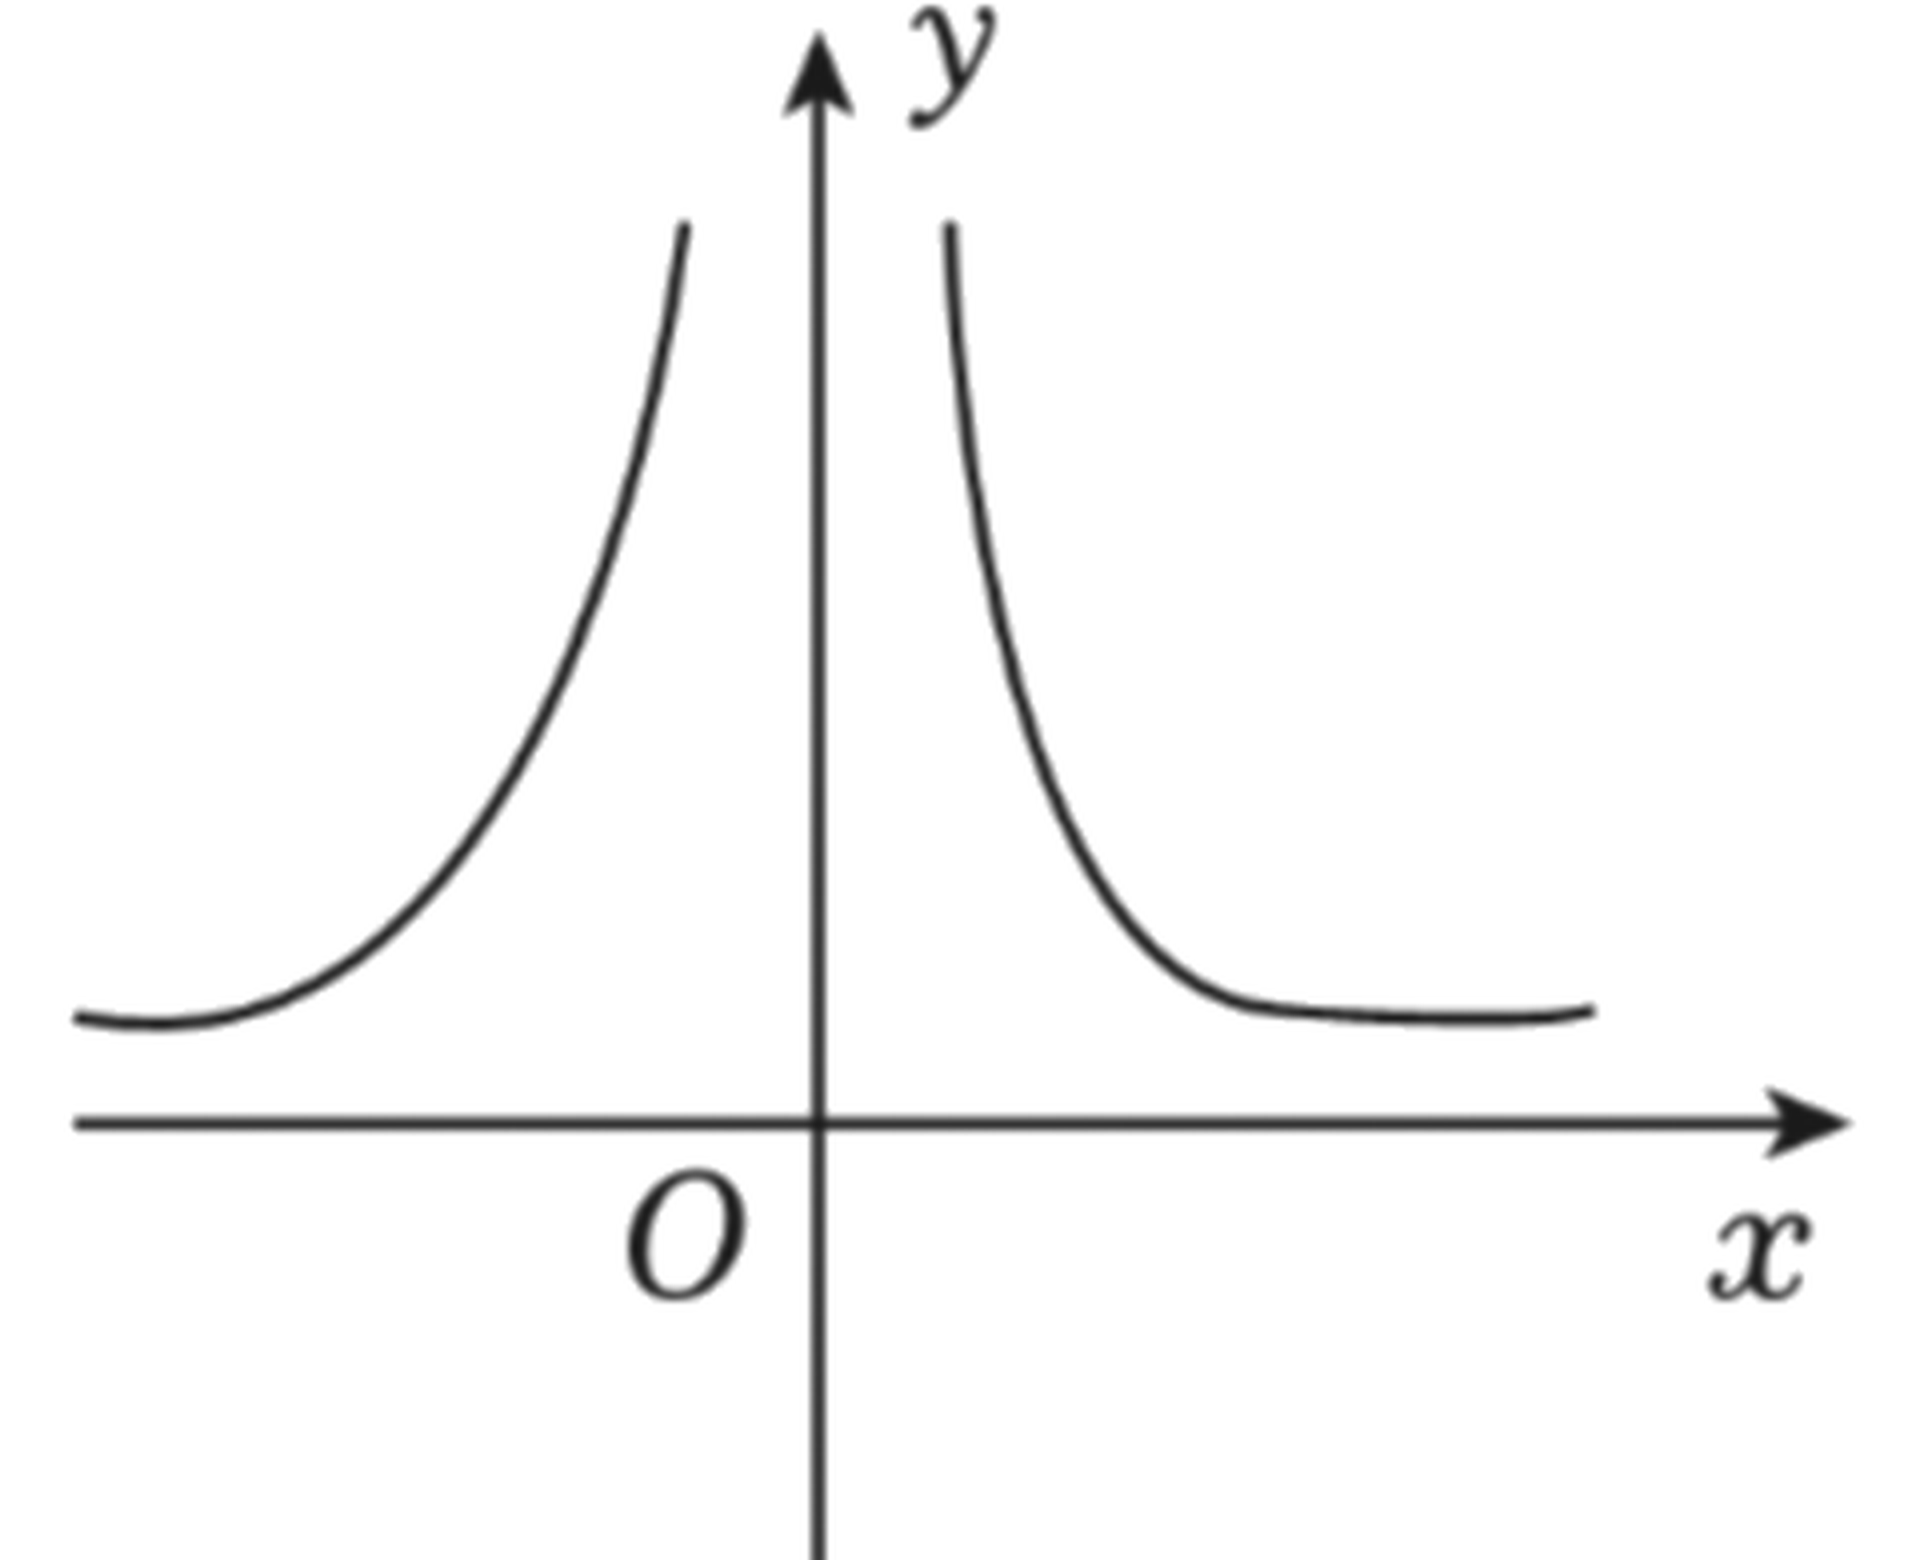
\includegraphics[width=0.36\textwidth]{figures/gao148_q16.png}
\end{center}

\ifanswer
\solbegin
\step{因为函数为偶函数，所以 $p$ 为偶数，且由图象形状判定 $\dfrac{p}{q}<0$.}
\step{又 $p$、$q$ 互质，所以 $q$ 为奇数. 故选 $D$.}
\solend
\fi

\end{enumerate}

\bigsec{三、解答题}

\begin{enumerate}
\setcounter{enumi}{16}

% === Q17 ===：\overline{B}／\varnothing／\R／\mid 逐处照录；解析 8 行
\item 已知集合 $A=\left\{x\mid \dfrac{5}{2x+1}>1\right\}$，$B=\{x\mid x^2+(a+3)x+3a<0,a\in\R\}$.

(1) 求 $A$.

(2) 若全集 $U=\R$，且 $A\cap\overline{B}=\varnothing$，求实数 $a$ 的取值范围.

\ifanswer
\solbegin
\step{(1) $\dfrac{5}{2x+1}>1$，即 $\dfrac{5}{2x+1}-1>0$，即 $\dfrac{4-2x}{2x+1}>0$，即 $(2x+1)(x-2)<0$，}
\step{解得 $-\dfrac{1}{2}<x<2$，所以 $A=\left(-\dfrac{1}{2},2\right)$；}
\step{(2) $x^2+(a+3)x+3a<0$，即 $(x+3)(x+a)<0$，}
\step{全集 $U=\R$，且 $A\cap\overline{B}=\varnothing$，}
\step{当 $a<3$ 时，解得 $-3<x<-a$，则 $\overline{B}=(-\infty,-3)\cup(-a,+\infty)$，}
\step{此时 $-a\geqslant2$，解得 $a\leqslant-2$，}
\step{当 $a\geqslant3$ 时，不满足 $A\cap\overline{B}=\varnothing$，}
\step{故实数 $a$ 的取值范围是 $(-\infty,-2]$.}
\solend
\fi

% === Q18 ===：cases 块整体算一个印刷行；解析 6 行
\item 已知幂函数经过点 $(2,4)$.

(1) 当 $x=\dfrac{1}{2}$ 时，求函数的值；

(2) 是否存在实数 $m$、$n$，使得该函数在区间 $[m,n]$ 上最小值为 $6m-8$，最大值为 $6n-8$？若存在，求出 $m$、$n$ 的值，若不存在，请说明理由.

\ifanswer
\solbegin
\step{(1) 设幂函数的解析式是 $y=x^\alpha$，则 $2^\alpha=4$，解得 $\alpha=2$，}
\step{故 $f(x)=x^2$，$f\left(\dfrac{1}{2}\right)=\dfrac{1}{4}$；}
\step{(2) 因为 $f(x)\geqslant0$，所以 $6m-8\geqslant0$，$m\geqslant\dfrac{4}{3}$，}
\step{由函数 $f(x)$ 在 $(0,+\infty)$ 严格增，得函数 $f(x)$ 在 $(m,n)$ 严格增，}
\step{所以 $\begin{cases}f(m)=6m-8\\f(n)=6n-8\end{cases}$ 且 $m<n$，解得 $m=2$，$n=4$，}
\step{故存在 $m=2$，$n=4$ 满足题意.}
\solend
\fi

% === Q19 ===：7 处评分档照 高一54／64 成例排 \dots\dots N 分；判别式高 \Delta；解析 9 行
\item 已知方程 $x^2+6mx+9m-2=0$，且 $x_1,x_2$ 是方程的两个不同的实数根.

(1) 若 $m=1$，求 $\dfrac{1}{x_1}+\dfrac{1}{x_2}$ 的值；

(2) 若 $m\in\R$，且 $x_1^2+x_2^2<4$，求 $m$ 取值范围.

\ifanswer
\solbegin
\step{(1) 当 $m=1$ 时，方程为 $x^2+6x+7=0$，\dots\dots1 分}
\step{则 $x_1+x_2=-6,x_1\cdot x_2=7$，\dots\dots2 分}
\step{$\dfrac{1}{x_1}+\dfrac{1}{x_2}=\dfrac{x_1+x_2}{x_1\cdot x_2}=-\dfrac{6}{7}$\dots\dots3 分}
\step{(2) $x_1+x_2=-6m,x_1\cdot x_2=9m-2$\dots\dots2 分}
\step{因为 $x_1^2+x_2^2=(x_1+x_2)^2-2x_1\cdot x_2$，所以 $(x_1+x_2)^2-2x_1\cdot x_2<4$，}
\step{所以 $36m^2-2(9m-2)<4$，解得 $0<m<\dfrac{1}{2}$\dots\dots2 分}
\step{又因为方程有两个不同的根，所以 $\Delta=36m^2-4(9m-2)>0$，}% 判别式原卷印等腰偏高粗三角 $\Delta$，照录（放大 07 页 q19_delta3.png／diag_band_q19.png 确认）
\step{解得 $m<\dfrac{1}{3}$ 或 $m>\dfrac{2}{3}$\dots\dots2 分}
\step{所以 $0<m<\dfrac{1}{3}$\dots\dots2 分}
\solend
\fi

% === Q20 ===：题目配图（矩形蔬菜温室，三版都出），\needvspace 守卫放 \item 之前；单位 \mathrm{m}／\mathrm{m}^2；解析 10 行
\needvspace{8cm}
\item 某村计划建造一个室内面积为 $600\mathrm{m}^2$ 的矩形蔬菜温室，在室内，沿左、右两侧与后侧内墙各保留 $2\mathrm{m}$ 宽的通道，沿前侧内墙保留 $4\mathrm{m}$ 宽的空地.

\begin{center}
% 矩形蔬菜温室示意图取 07 页右侧，去粉色水印、去色、4× LANCZOS 放大；三版都出
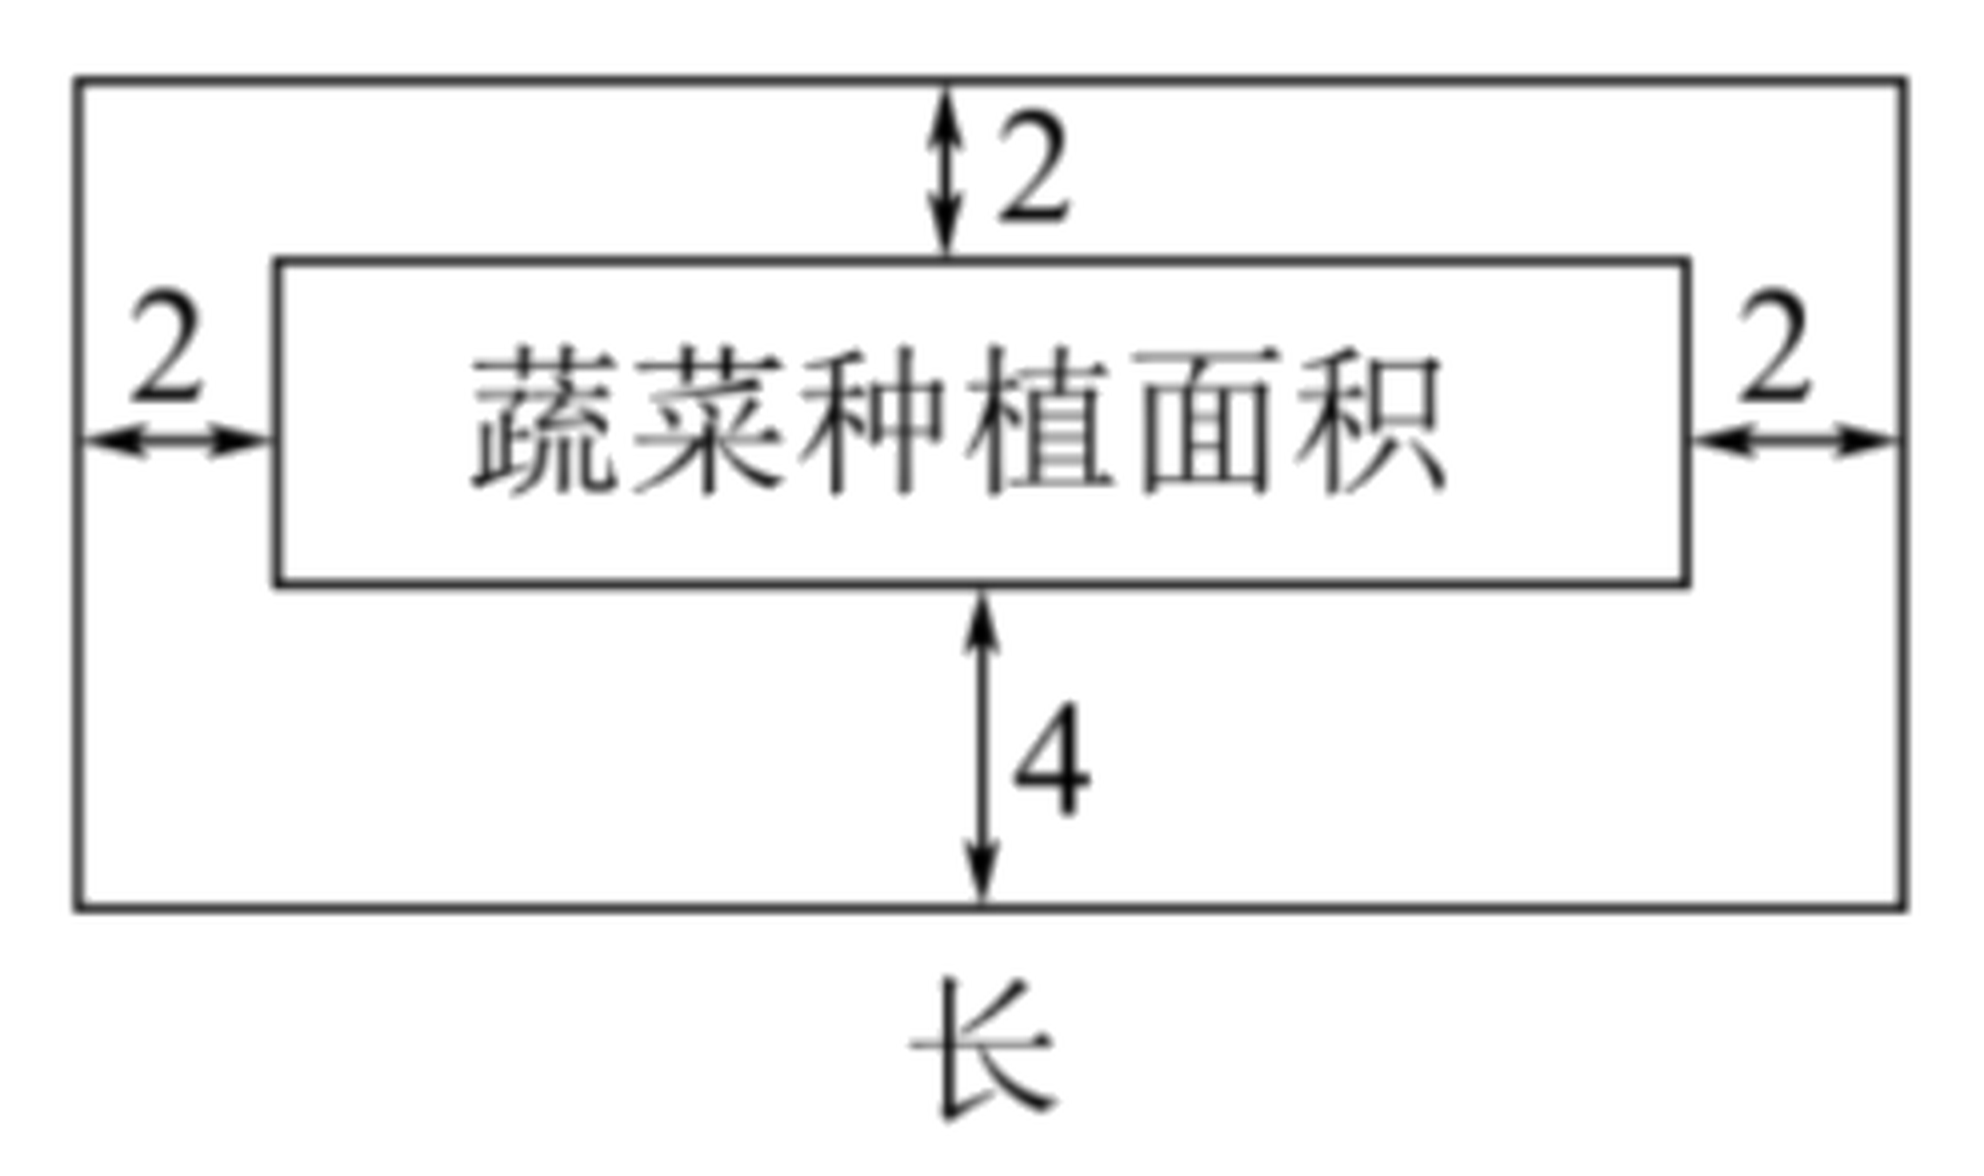
\includegraphics[width=0.45\textwidth]{figures/gao148_q20.png}
\end{center}

(1) 写出蔬菜的种植面积关于矩形温室的长之间的关系式.

(2) 当矩形温室的边长各为多少时，蔬菜的种植面积最大？最大种植面积是多少？

\ifanswer
\solbegin
\step{(1) 设蔬菜的种植面积为 $y\mathrm{m}^2$，矩形温室的长为 $x\mathrm{m}$，}
\step{则矩形温室的宽为 $\dfrac{600}{x}\mathrm{m}$，}
\step{种植蔬菜矩形的长为 $(x-4)\mathrm{m}$，宽为 $\left(\dfrac{600}{x}-6\right)\mathrm{m}$，}
\step{所以 $y=(x-4)\left(\dfrac{600}{x}-6\right)(4<x<100)$；}
\step{(2) 因为 $y=(x-4)\left(\dfrac{600}{x}-6\right)=624-\left(6x+\dfrac{2400}{x}\right)$，}
\step{因为 $6x+\dfrac{2400}{x}\geqslant2\sqrt{6x\cdot\dfrac{2400}{x}}=240$，}
\step{当且仅当 $6x=\dfrac{2400}{x}$，即 $x=20$ 时取等号，}
\step{所以 $y=624-\left(6x+\dfrac{2400}{x}\right)\leqslant624-240=384$.}
\step{即当矩形温室的一边长为 $20\mathrm{m}$，另一边长为 $30\mathrm{m}$ 时，}
\step{蔬菜的种植面积最大，最大为 $384\mathrm{m}^2$.}
\solend
\fi

% === Q21 ===：3 问、cases 块整体算一个印刷行；判别式高 \Delta；解析 19 行（末行续 09 页）
\item 二次函数 $f(x)=ax^2+bx+c$ 满足对任意的 $x\in\R$，$x-1\leqslant f(x)\leqslant x^2-x$ 恒成立.

(1) 求证：$f(1)$ 为定值；

(2) 若 $f(0)=-\dfrac{1}{4}$，求二次函数 $f(x)$ 的表达式；

(3) 求 $a+2b+5c$ 的取值范围.

\ifanswer
\solbegin
\step{(1) 对任意的 $x\in\R$，$x-1\leqslant f(x)\leqslant x^2-x$ 恒成立，则 $0\leqslant f(1)\leqslant0$，}
\step{所以 $f(1)=0$，为定值.}
\step{(2) 由(1)得 $a+b+c=f(1)=0$，由 $f(0)=-\dfrac{1}{4}$，得 $c=-\dfrac{1}{4}$，}
\step{则 $b=\dfrac{1}{4}-a$，$f(x)=ax^2+\left(\dfrac{1}{4}-a\right)x-\dfrac{1}{4}$，}
\step{不等式 $x-1\leqslant f(x)$ 可化为 $ax^2+\left(\dfrac{1}{4}-a\right)x-\dfrac{1}{4}\geqslant x-1$，}
\step{即 $ax^2-\left(a+\dfrac{3}{4}\right)x+\dfrac{3}{4}\geqslant0$，}
\step{一元二次不等式 $ax^2-\left(\dfrac{3}{4}+a\right)x+\dfrac{3}{4}\geqslant0$ 恒成立，则 $\begin{cases}a>0\\\Delta=\left(a+\dfrac{3}{4}\right)^2-3a\leqslant0\end{cases}$，}% 判别式原卷印等腰偏高粗三角 $\Delta$，照录（放大 08 页 q21_delta3.png／diag_band_q21.png 确认）
\step{解得 $a=\dfrac{3}{4}$，}
\step{此时 $f(x)=\dfrac{3}{4}x^2-\dfrac{1}{2}x-\dfrac{1}{4}$，$x^2-x-f(x)=\dfrac{1}{4}(x-1)^2\geqslant0$ 恒成立，}
\step{所以 $f(x)=\dfrac{3}{4}x^2-\dfrac{1}{2}x-\dfrac{1}{4}$.}
\step{(3) 由(1)得 $b=-a-c$，$f(x)=ax^2-(a+c)x+c=(ax-c)(x-1)$，}
\step{不等式 $x-1\leqslant f(x)$ 可化为 $(x-1)(ax-c-1)\geqslant0$，}
\step{一元二次不等式 $(x-1)(ax-c-1)\geqslant0$ 恒成立，则 $a>0$，}
\step{且方程 $(x-1)(ax-c-1)=0$ 有相等的实数根，因此 $c=a-1$，$a>0$，}
\step{不等式 $f(x)\leqslant x^2-x\Leftrightarrow(ax-c)(x-1)\leqslant x^2-x\Leftrightarrow(x-1)[(1-a)x+c]\geqslant0$，}
\step{同理 $1-a>0$，且方程 $(x-1)[(1-a)x+c]=0$ 有相等的实数根，}
\step{因此 $c=a-1$，$a<1$，从而 $c=a-1$，$b=1-2a$，$0<a<1$，}
\step{$a+2b+5c=a+2(1-2a)+5(a-1)=2a-3\in(-3,-1)$，}
\step{所以 $a+2b+5c$ 的取值范围是 $(-3,-1)$.}
\solend
\fi

\end{enumerate}

\end{document}
"
%
% ① 原始材料：微信公众号"魔都数学加油站"文章，连载"27学年高一148"，原文标题
% "27学年高一148——2026-2027年上海市新川中学高一上期中"（2026-11-21 推送）；
% 原文链接：https://mp.weixin.qq.com/s/Alhmwb3sSLQMp_wjzoAVyA 。
% 正文为 9 张 PNG 页（01/03/04/07/08/09 为 2560×3620，02/05/06 为 4762×6735，
% 同一篇各页分辨率混排，逐页按各自分辨率裁图核对，别按预览比例换算裁框）。
% 体例：混合体例讲评版——19 题中 Q4、Q5 只印【答案】、无【解析】；Q13 的答案"C"
% 直接印在题干括号内、无【答案】/【解析】段；其余 16 题印【解析】（逐题核实，见 ② ②）。
% 题目、答案、解析均据原图转录；卷面粉红色水印"魔都数学加油站"及公众号页脚未录入。
% 全卷插图清单（逐页通读 9 页确认）：4 幅题目配图，均三版都出、均非【解析】内配图：
%   · Q12 幂函数曲线族图（03 页右侧：x/y 轴、O、A(1,0)、B(0,1)、M、N 与两族
%     y=x^α／y=x^β 曲线、线段 AB、虚线），题干"（如图）"处，裁 figures/gao148_q12.png；
%   · Q15 四条指数函数曲线图（04 页右侧：①②③④ 四曲线同过 (0,1)、x/y 轴、O、
%     y 轴刻度 1），题干"如图"处，裁 figures/gao148_q15.png；
%   · Q16 关于 y 轴对称的幂函数曲线图（04 页右下：x/y 轴、O、两支上翘曲线），
%     题干"如图所示"处，裁 figures/gao148_q16.png；
%   · Q20 矩形蔬菜温室示意图（07 页右侧：大矩形＋内框"蔬菜种植面积"＋2/2/4
%     通道标注＋"长"），题干处，裁 figures/gao148_q20.png；
%   其余各页逐页确认无其它题目配图、无【解析】内配图、无表格，亦无"题干写如图而
%   源码漏图"一处；Q19 解析行末的虚线"----N 分"为评分档（非图），Q18／Q21 的
%   cases 块为数学块（非图）。4 图均取自原卷截图，去粉色水印、去色、4× LANCZOS 放大。
%
% 卷首标题：原卷印作"2026-2027 年新川中学高一上期中"，年份区间按全稿惯例排 en dash；
% 原卷卷面未印副标题，本稿按同期中卷（高一140／141／143／144／145／146／147）知识模块
% 口径补出"集合与常用逻辑用语、不等式、函数"。
%
% 题号体例（逐页核实定稿）：本卷共 19 题——一、填空题 3—12（10 题）、
% 二、选择题 13—16（4 题）、三、解答题 17—21（5 题）。
% 三节分别 \setcounter{enumi}{2}／{12}／{16}。原卷从第 3 题起、无第 1、2 题，
% 本稿保留原题号；全卷无附加题节、无 Q22（Q21 解析末行"所以 a+2b+5c 的取值范围是
% (-3,-1)."为全卷收尾，09 页下半仅水印、无正文）。
%
% ② 与原卷的排版差异：
%   ① 原文从第 3 题起，本稿保留原题号；共 19 题三节；
%   ② 混合体例逐题核实：Q4（反证法"假设的内容"）、Q5 只印【答案】、无【解析】，
%      按 高一140 第 5 题／高一145 Q3 成例提 \ans{}、不补造解析；Q13 答案"C"直接
%      印在题干括号内（" ( C ) "）、全卷无该题【答案】/【解析】段，按 高一84 Q13／
%      高一37 Q13／高一53 Q13 成例括号 \mbox{（\quad）} 留空、另提 \ans{$C$}；
%      其余 16 题印【解析】、用 \solbegin…\solend，选择题答案在解析末句"故选 X"
%      （Q14 选 D、Q15 选 B、Q16 选 D，逐个放大原图核实）、题干括号留空、不另提
%      \ans{}；答案版【答案】/【解析】标记数 = 19（3 个 \ans ＋ 16 个 \solbegin）
%      = 全卷题数；
%   ③ 原卷卷面未印副标题，本稿按知识模块口径补出；
%   ④ 原卷填空横线按全稿惯例排 \blankline[4.4em]；选择题括号排 \mbox{（\quad）}、
%      选项段前按惯例加 \keepwithprev；Q13／Q16 四选项为两行两列、Q14／Q15 选项
%      为一行，照原卷分行；解答题不留作答区、不加 \anspace（原卷为讲评版，
%      与 129／131／132／133／136／140／141／143／144／145／146 同）；
%   ⑤ 数集：Q11"在 R 上定义运算"、Q13"x、y∈R"、Q16"p、q∈Z"、Q17"a∈R"
%      "U=R"、Q19"m∈R"、Q21"x∈R" 原卷印斜体 R/Z，按全稿惯例统一改 \R／\Z
%      （本卷未出现 N，\N^* 无对应处）；绝对值排 \lvert…\rvert（Q9／Q14），
%      集合描述竖线排 \mid（Q17）；不等号按全稿惯例排 \leqslant／\geqslant；
%      补集照原卷上划线排 \overline{B}（Q17 题干 1 处＋解析 3 处）；空集
%      \varnothing（Q17 题干 1 处＋解析 2 处）；\subset（Q3 题干 {a}⊂M）与
%      \subseteq（Q3 题干 M⊆{a,b,c,d}）逐处照录不统一（放大 01 页 q3_subset.png）；
%   ⑥ 子题标号 (1)(2)(3) 半角括号照录；圈数字 ①—⑥ 在文本模式（Q14 六个结论、
%      Q15 曲线编号与其解析、Q14 解析"对①…对⑥"），按 common.sty 划入 CJK 字符类
%      渲染；cases 块整体算一个印刷行；\left…\right 不得拆到不同 $…$ 组；
%      单位 m／m² 排 \mathrm{m}／\mathrm{m}^2（Q20，原卷印正体 m）；
%   ⑦ 题干／解析中的中文弯引号按原卷照录：Q4" ab 可以被 5 整除，那么 a、b 中
%      至少有一个能被 5 整除 "（开引号后有空格、闭引号后空格接"时"）、
%      Q13" x=0 "" xy=0 "（引号内空格），注释内一律 ASCII 引号；
%   ⑧ 半角逗号在数学组之间是全稿惯例、非笔误（Q3"{a,b,c,d}"、Q6"$x,y$"
%      "$x=\frac13,y=\frac16$"、Q10、Q11"$a=-2,b=-1"、Q12"$\alpha=\log..,\beta=..$"、
%      Q14"$a+b<0,a-b<0$"、Q17、Q19"$x_1+x_2=-6,x_1\cdot x_2=7$"、Q20、Q21 等），
%      逐处照录别改全角；行末西文句点照录为 ASCII `.`；行中全角逗号／顿号照录；
%   ⑨ "图像／图象"逐处放大核：全卷 9 处均印"图象"（象，无亻）、未见"图像"，
%      逐处照录未统一改动（Q8 题干/解析各 1、Q12 题干 2、Q15 题干 1／解析 2、
%      Q16 题干 1／解析 1；放大 02/03/04/05 页 /tmp/gao148/zoom/my_wide_a.png、
%      my_wide_b.png 与宋体参考"象／像"并排确认）；
%   ⑩ 判别式 Δ/△ 混用是照录项：Q11 解析"△=1−4(−a²+a+1)<0"印扁等边空心
%      三角 \triangle；Q19 解析"Δ=36m²−4(9m−2)>0"、Q21 解析 cases 块
%      "Δ=(a+3/4)²−3a≤0" 两处印等腰偏高粗三角 \Delta，逐处放大判断、照录
%      不统一（参照 高一142／144／145 头注④口径，详见 ④）；
%   ⑪ 一条 \step = 原卷解析的一个印刷行，cases 块整体算一个印刷行；别把原卷折行
%      并起来、别把一行拆多条。Q3 六行、Q7 五行（01 页末首行＋02 页顶四行）、
%      Q9 七行、Q11 五行、Q14 八行（对② 的两行公式各占一印刷行）、Q17 八行、
%      Q18 六行、Q19 九行（7 处评分档附在行末）、Q20 十行、Q21 十九行
%      均按印刷行逐条断，不丢行；
%   ⑫ 配图：4 幅均为题目配图（三版都出），放 \item 内题干之后 \begin{center}；
%      大图块加 \needvspace 守卫把整块推走（守卫放 \item 之前，见 高一145 Q14/Q20
%      成例与切页审计 B 类坑）；三版切页审计均"合计异常：无"；
%   ⑬ 跨页续印按题合并：Q3/4/5 在 01 页；Q6 题干＋解析在 01 页；Q7 题干在 01 页
%      末、解析首行在 01 页末续 02 页顶四行；Q8/9/10 在 02 页（Q9 解析续 02 页下半、
%      Q10 题干与解析前 2 行在 02 页末）；Q10 解析末行续 03 页顶；Q11/12 在 03 页、
%      "二、选择题"标题与 Q13/14 题干在 03 页下半；Q13 无解析；Q14 解析在 04 页顶、
%      Q15 题干＋图＋选项＋解析在 04 页、Q16 题干＋图在 04 页末；Q16 选项＋解析＋
%      "三、解答题"标题＋Q17 题干＋解析在 05 页、Q18 题干首句在 05 页末；Q18 题干
%      续＋解析、Q19 题干＋解析前 5 行在 06 页；Q19 解析续 4 行＋Q20 题干＋图＋
%      解析（10 行全部）在 07 页，末行"蔬菜的种植面积最大，最大为 384m²."收尾；
%      Q21 题干＋解析前 18 行在 08 页；Q21 解析末行"所以 a+2b+5c 的取值范围是
%      (-3,-1)."在 09 页上半（09 页下半仅水印、无正文）。本稿按题连排，不丢行、
%      不并折行；
%   ⑭ 原卷解析内无红色"法一／法二"之类小标题，故本卷无 \stepm；水印
%      "魔都数学加油站"红色不录入；Q19 解析 7 处评分档（1/2/3/2/2/2/2 分）
%      原卷在行末印一串虚线，本稿照 高一54／64 成例排 \dots\dots N 分，
%      分值逐处照录、位置不变。
%
% ③ 行数复核：一条 \step／\stepm = 原卷解析的一个印刷行，cases 块作一个印刷行计。
%   逐题数（主会话逐页核对定稿）：Q3：6；Q4：0（只印【答案】、提 \ans{}）；
%   Q5：0（只印【答案】、提 \ans{}）；Q6：2；Q7：5；Q8：2；Q9：7；Q10：3；
%   Q11：5；Q12：2；Q13：0（答案印在题干括号内、另提 \ans{}）；Q14：8；Q15：5；
%   Q16：2；Q17：8；Q18：6；Q19：9；Q20：10；Q21：19。
%   合计 99 条 \step（本卷无 \stepm：解析内无红色"法一／法二"类小标题），
%   与原卷逐题印刷行相等。全卷 16 题设 \solbegin…\solend ＋ 3 处 \ans{}，
%   答案版【答案】/【解析】标记数 = 19 = 全卷题数。
%
% ④ 判别式／子集符号结论（逐处放大原图照录、不得统一，主会话像素级复核）：
%   判别式全卷 3 处，两形混用逐处照录不统一（参照 高一142／144／145 头注④口径）：
%     · Q11 解析"△=1−4(−a²+a+1)<0" 原卷印扁等边空心三角（宽>高、细线），
%       照录 \triangle（放大 03 页 /tmp/gao148/zoom/q11_delta3.png、
%       delta_montage.png 确认）；
%     · Q19 解析"Δ=36m²−4(9m−2)>0" 原卷印等腰偏高粗三角（高>宽），
%       照录 \Delta（放大 07 页 /tmp/gao148/zoom/q19_delta3.png 确认）；
%     · Q21 解析 cases 块"Δ=(a+3/4)²−3a≤0" 原卷印等腰偏高粗三角（高>宽），
%       照录 \Delta（放大 08 页 /tmp/gao148/zoom/q21_delta3.png 确认）。
%   子集／补集：Q3 题干"{a}⊂M⊆{a,b,c,d}" 前者印单线 ⊂、无下划线，照录 \subset；
%     后者印带下划线 ⊆，照录 \subseteq（放大 01 页 /tmp/gao148/zoom/q3_subset.png
%     确认）；Q17 题干 1 处＋解析 3 处共 4 处 \overline{B} 照原卷上划线
%     （B 上横线、非 C_U B）；空集 \varnothing 3 处（Q17 题干 1 处、解析 2 处）；
%     Q17 集合描述竖线 \mid；数集 \R／\Z 归一见 ② ⑤。
%
% ⑤ 存疑照录（放大原图确认，照录未改、正文对应处另有 % 注）：
%   1. Q3 解析末行"所以 M 一共有 3+3+1+1=8 个" 原卷印 $3+3+1+1=8$，按上文
%      四行应为 $1+3+3+1=8$（疑为原卷加数顺序笔误，和仍为 8），放大 01 页
%      /tmp/gao148/zoom/my_q3_sol.png 确认，照录未改。
%   2. Q13 答案"C"直接印在题干括号内、全卷无该题【答案】/【解析】段，按
%      高一84 Q13 成例括号留空、另提 \ans{$C$}（见 ② ②），未补造解析。
%   3. Q19 解析 7 处评分档（"----N 分"）原卷印一串虚线，本稿照 高一54／64
%      成例排 \dots\dots N 分，分值逐处照录、位置不变。
%   4. 判别式 Q11 扁 \triangle 与 Q19／Q21 高 \Delta 两形混用，逐处照录不统一（见 ④）。
%   5. "图像／图象"全卷 9 处均印"图象"、未见"图像"（见 ② ⑨），逐处放大核实照录，
%      未统一改动。
%   全卷除此 5 类外未发现其它笔误／自相矛盾处。
%
% ⑥ 跨页续印按题合并说明：见 ② ⑬。
%
\documentclass[a4paper,11pt]{article}
\usepackage{common}

\begin{document}

\examtitlest[3]{2026--2027 年新川中学高一上期中}{集合与常用逻辑用语、不等式、函数}

\bigsec{一、填空题}

\begin{enumerate}
\setcounter{enumi}{2}

% === Q3 ===：题干 {a}⊂M⊆{a,b,c,d} 两个子集符号逐处照录；解析 6 行
\item 满足 $\{a\}\subset M\subseteq\{a,b,c,d\}$ 的集合 $M$ 有\blankline[4.4em]个.

\ifanswer
\solbegin
\step{$M$ 是 $\{a,b,c,d\}$ 的子集，但必含有元素 $a$，}
\step{当 $M$ 中只一个元素时，$M=\{a\}$ 只有 1 个；}
\step{当 $M$ 中有二个元素时，$M$ 有 3 个；}
\step{当 $M$ 中有三个元素时，$M$ 有 3 个；}
\step{当 $M$ 中有四个元素时，$M$ 有 1 个；}
\step{所以 $M$ 一共有 $3+3+1+1=8$ 个.}% 原卷印 $3+3+1+1=8$（按上文四行应为 $1+3+3+1$），疑为加数顺序笔误，照录未改（放大 01 页 my_q3_sol.png）
\solend
\fi

% === Q4 ===：原卷只印【答案】、无【解析】，按 高一140 第 5 题成例提 \ans{}；弯引号与空格照录
\item 用反证法证明命题 “ $ab$ 可以被 5 整除，那么 $a$、$b$ 中至少有一个能被 5 整除” 时假设的内容应该是\blankline[4.4em].

\ifanswer
\ans{$a$、$b$ 都不能被 5 整除}
\fi

% === Q5 ===：原卷只印【答案】 $[-2,1)$、无【解析】，提 \ans{}
\item 不等式 $\dfrac{x+2}{x-1}\leqslant0$ 的解集为\blankline[4.4em].

\ifanswer
\ans{$[-2,1)$}
\fi

% === Q6 ===：解析 2 行；半角逗号在数学组之间照录
\item 设 $x,y\in(0,+\infty)$，且 $x+4y=1$，则 $\dfrac{1}{x}+\dfrac{1}{y}$ 的最小值为\blankline[4.4em].

\ifanswer
\solbegin
\step{因为 $\dfrac{1}{x}+\dfrac{1}{y}=(x+4y)\left(\dfrac{1}{x}+\dfrac{1}{y}\right)=5+\dfrac{4y}{x}+\dfrac{x}{y}\geqslant5+2\sqrt{\dfrac{4y}{x}\cdot\dfrac{x}{y}}=9$，}
\step{当且仅当 $\dfrac{4y}{x}=\dfrac{x}{y}$，即 $x=2y$，即 $x=\dfrac{1}{3},y=\dfrac{1}{6}$ 时取等号，故最小值为 9.}
\solend
\fi

% === Q7 ===：题干在 01 页末、解析首行在 01 页末续 02 页顶四行；解析 5 行
\item 若不等式 $x^2+ax+b<0$ 的解集为 $(-3,-1)$，则不等式 $bx^2+ax+1\leqslant0$ 的解集为\blankline[4.4em].

\ifanswer
\solbegin
\step{不等式 $x^2+ax+b<0$ 的解集为 $(-3,-1)$，}
\step{所以方程 $x^2+ax+b=0$ 的两个实数根为 $-3$ 和 $-1$，}
\step{由根与系数的关系得 $a=4$，$b=3$，}
\step{故 $bx^2+ax+1\leqslant0$ 可化为 $3x^2+4x+1\leqslant0$，解得 $-1\leqslant x\leqslant-\dfrac{1}{3}$，}
\step{所求不等式 $bx^2+ax+1\leqslant0$ 的解集为 $\left[-1,-\dfrac{1}{3}\right]$.}
\solend
\fi

% === Q8 ===："图象"照录；解析 2 行
\item 函数 $y=a^{x-2}+2(a>0,a\ne1)$ 的图象必经过定点\blankline[4.4em].

\ifanswer
\solbegin
\step{令 $x-2=0$，得 $x=2$，则 $y=a^0+2=3$，}
\step{所以函数 $y=a^{x-2}+2$ 的图象过定点 $(2,3)$.}
\solend
\fi

% === Q9 ===：解析 7 行；首句末西文句点照录
\item 不等式 $\lvert x+3\rvert+\lvert a-x\rvert>6$ 对一切实数 $x$ 恒成立，则实数 $a$ 的取值范围为\blankline[4.4em].

\ifanswer
\solbegin
\step{$\lvert x+3\rvert$ 表示 $x$ 到 $-3$ 的距离，$\lvert a-x\rvert$ 表示 $x$ 到 $a$ 的距离.}
\step{所以它们的和为 $x$ 到 $-3$ 和 $x$ 到 $a$ 的距离之和，}
\step{当 $x$ 位于 $-3$ 和 $a$ 之间时，距离和取得最小值，}
\step{即两点之间的距离 $\lvert a-(-3)\rvert=\lvert a+3\rvert$，}
\step{若最小值 $\lvert a+3\rvert>6$，则原式对所有 $x$ 恒成立.}
\step{解得 $a+3>6$ 或 $a+3<-6$，即 $a>3$ 或 $a<-9$，}
\step{故 $a\in(3,+\infty)$ 或 $a\in(-\infty,-9)$.}
\solend
\fi

% === Q10 ===：题干与解析前 2 行在 02 页末、解析末行续 03 页顶；解析 3 行
\item 已知 $2^a=3$，$\log_3 5=b$，则 $\log_{15}20=$\blankline[4.4em]（用 $a$、$b$ 表示）.

\ifanswer
\solbegin
\step{因为 $2^a=3$，所以 $a=\log_2 3=\dfrac{\lg3}{\lg2}$，又 $\log_3 5=b=\dfrac{\lg5}{\lg3}$，}
\step{所以 $\lg3=a\lg2$，$\lg5=b\lg3=ba\lg2$，}
\step{则 $\log_{15}20=\dfrac{2\lg2+\lg5}{\lg3+\lg5}=\dfrac{2\lg2+ab\lg2}{a\lg2+ab\lg2}=\dfrac{2+ab}{a+ab}$.}
\solend
\fi

% === Q11 ===：在 \R 上定义运算 \otimes；判别式扁 \triangle 照录；解析 5 行
\item 在 $\R$ 上定义运算 $\otimes:x\otimes y=x(1-y)$，若不等式 $(x-a)\otimes(x+a)<1$ 对任意实数 $x$ 恒成立，则 $a$ 的取值范围是\blankline[4.4em].

\ifanswer
\solbegin
\step{由题意得不等式 $(x-a)\otimes(x+a)<1$ 对任意实数 $x$ 恒成立，}
\step{即不等式 $(x-a)(1-x-a)<1$ 对任意实数 $x$ 恒成立，}
\step{即 $x^2-x-a^2+a+1>0$ 对任意实数 $x$ 恒成立，}
\step{所以 $\triangle=1-4(-a^2+a+1)<0$，解得 $-\dfrac{1}{2}<a<\dfrac{3}{2}$，}% 判别式原卷印扁等边空心三角 $\triangle$，照录（放大 03 页 q11_delta3.png 确认）
\step{所以实数 $a$ 的取值范围为 $\left(-\dfrac{1}{2},\dfrac{3}{2}\right)$.}
\solend
\fi

% === Q12 ===：题目配图（幂函数曲线族，三版都出）；"图象"照录；解析 2 行
\needvspace{8cm}
\item 幂函数 $y=x^\alpha$，当 $\alpha$ 取不同的正数时，在区间 $[0,1]$ 上它们的图象是一族美丽的曲线（如图）. 设点 $A(1,0)$，$B(0,1)$，连接 $AB$，线段 $AB$ 恰好被其中的两个幂函数 $y=x^\alpha$，$y=x^\beta$ 的图象三等分，即有 $BM=MN=NA$，那么 $\alpha\beta=$\blankline[4.4em].

\begin{center}
% 幂函数曲线族图取 03 页右侧，去粉色水印、去色、4× LANCZOS 放大；三版都出
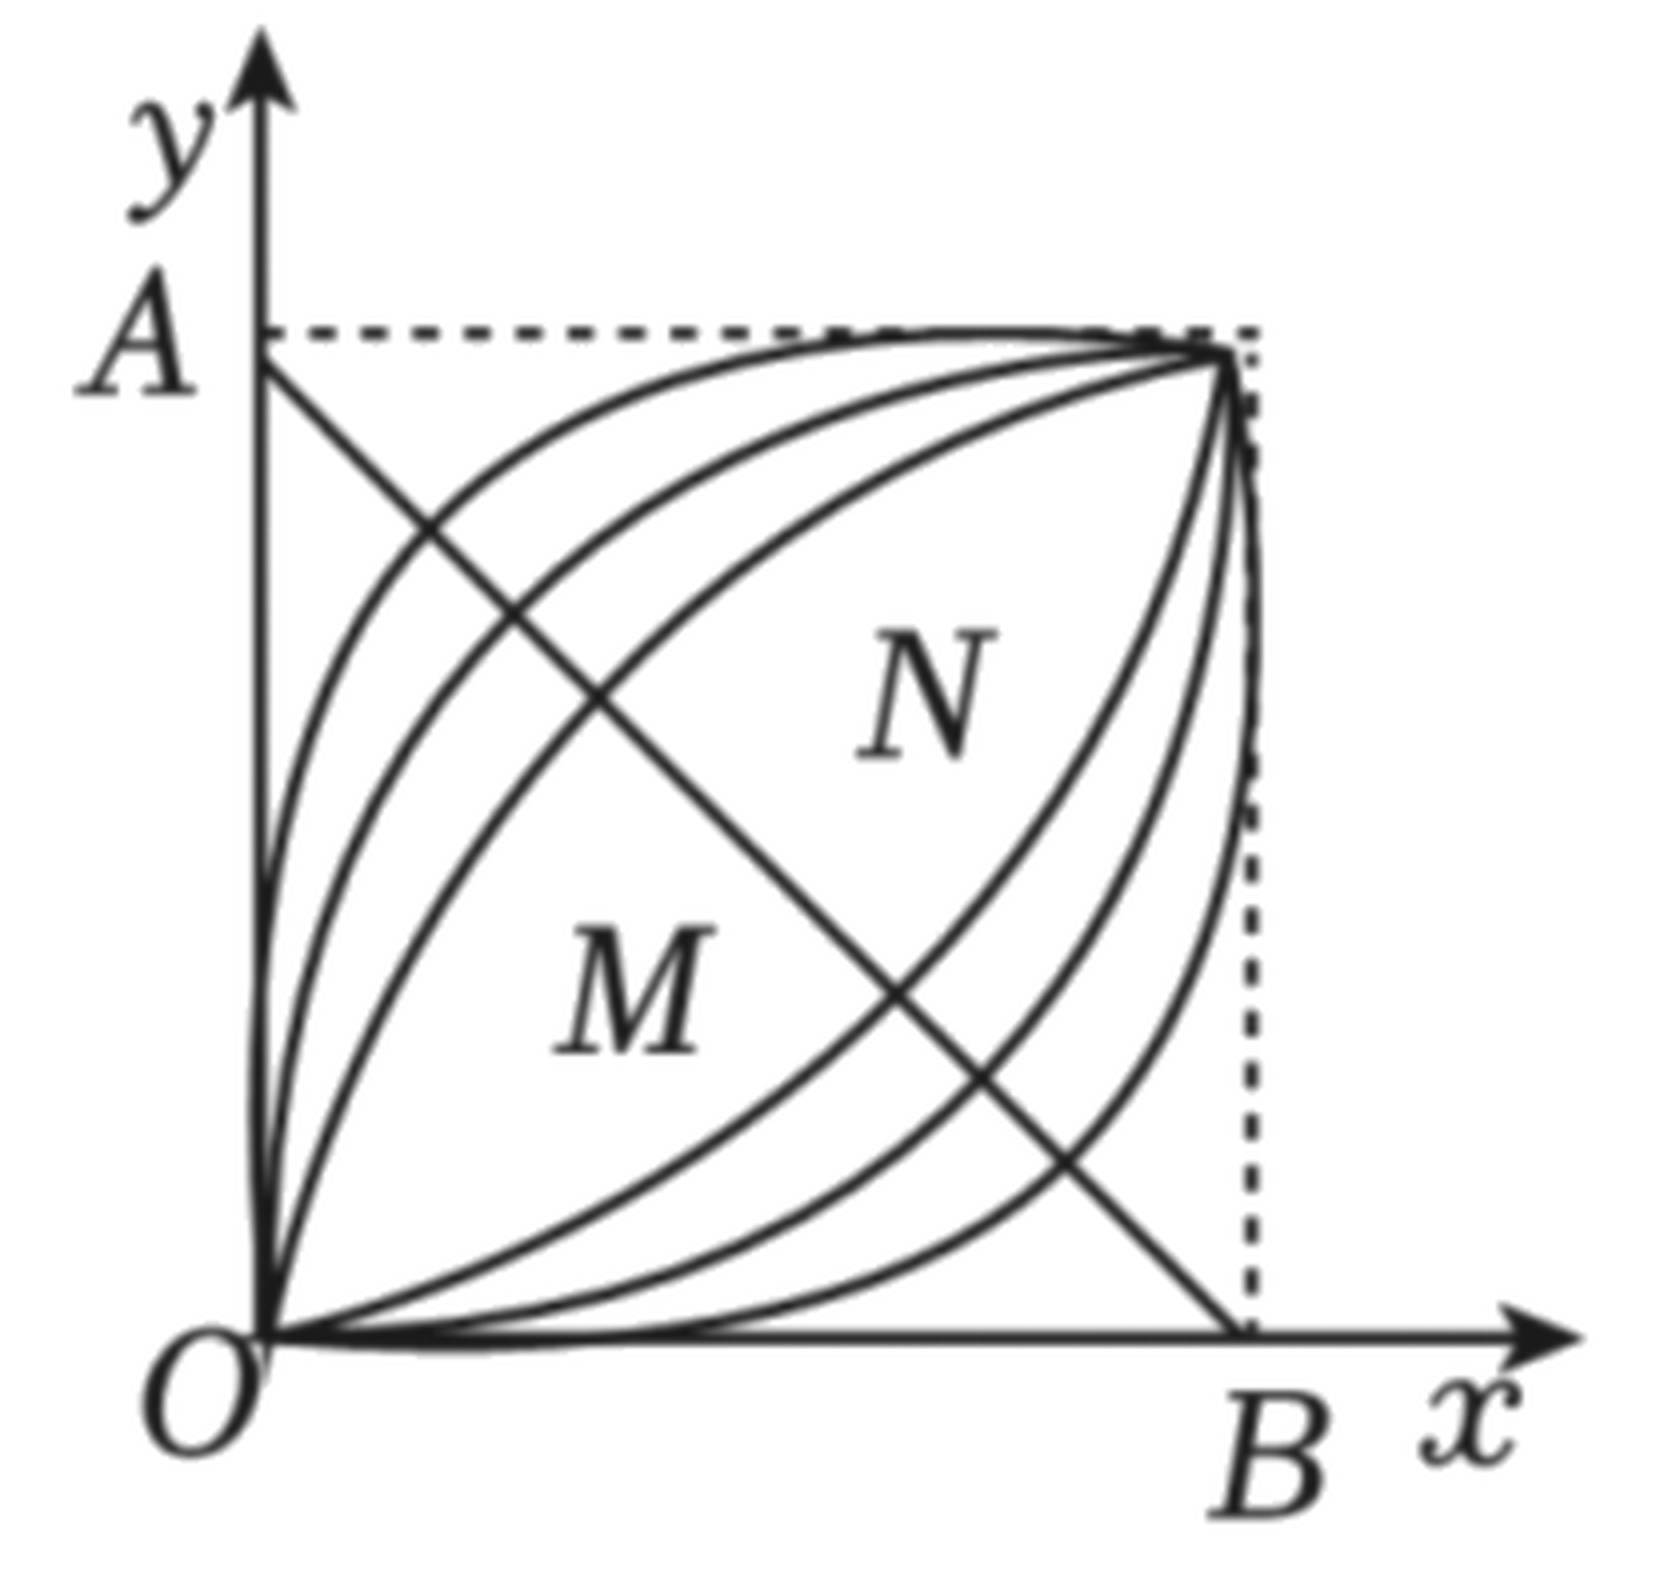
\includegraphics[width=0.40\textwidth]{figures/gao148_q12.png}
\end{center}

\ifanswer
\solbegin
\step{$BM=MN=NA$，点 $A(1,0)$，$B(0,1)$，所以 $M\left(\dfrac{1}{3},\dfrac{2}{3}\right)$，$N\left(\dfrac{2}{3},\dfrac{1}{3}\right)$，}
\step{分别代入 $y=x^\alpha$，$y=x^\beta$，$\alpha=\log_{\frac{2}{3}}\dfrac{1}{3},\beta=\log_{\frac{1}{3}}\dfrac{2}{3}$，$\alpha\beta=\log_{\frac{1}{3}}\dfrac{2}{3}\cdot\log_{\frac{2}{3}}\dfrac{1}{3}=1$.}
\solend
\fi

\end{enumerate}

\bigsec{二、选择题}

\begin{enumerate}
\setcounter{enumi}{12}

% === Q13 ===：答案"C"直接印在题干括号内、全卷无该题【答案】/【解析】段，按 高一84 Q13 成例括号留空、另提 \ans{$C$}；弯引号含空格
\item 若 $x$、$y\in\R$，则 “ $x=0$ ” 是 “ $xy=0$ ” 的\mbox{（\quad）}

\keepwithprev
A. 充要条件\qquad\qquad B. 必要不充分条件

C. 充分不必要条件\qquad\qquad D. 既不充分也不必要条件

\ifanswer
\ans{$C$}
\fi

% === Q14 ===：六个结论（圈数字在文本模式）、四选项一行；解析 8 行（对② 的两行公式各占一印刷行）
\item 若 $a<b<0$，下面有六个结论：① $a^2>b^2$；② $a^3<b^3$；③ $\dfrac{1}{a}<\dfrac{1}{b}$；④ $\dfrac{a}{b}>1$；⑤ $\dfrac{1}{a-b}>\dfrac{1}{a}$；⑥ $\lvert a\rvert>-b$. 其中正确的个数是\mbox{（\quad）}

\keepwithprev
A. 1\qquad\qquad B. 2\qquad\qquad C. 3\qquad\qquad D. 4

\ifanswer
\solbegin
\step{对①：$a^2-b^2=(a+b)(a-b),a+b<0,a-b<0$，故 $a^2-b^2>0$，正确；}
\step{对②：$a^3-b^3=(a-b)(a^2+ab+b^2)=(a-b)\left[\left(a+\dfrac{1}{2}b\right)^2+\dfrac{3}{4}b^2\right],a-b<0$，}
\step{$\left(a+\dfrac{1}{2}b\right)^2+\dfrac{3}{4}b^2>0$，故 $a^3-b^3<0$，正确；}
\step{对③：取 $a=-2,b=-1$，则 $\dfrac{1}{a}=-\dfrac{1}{2},\dfrac{1}{b}=-1,\dfrac{1}{a}>\dfrac{1}{b}$，错误；}
\step{对④：$\dfrac{a}{b}-1=\dfrac{a-b}{b},a-b<0,b<0$，故 $\dfrac{a}{b}-1>0$，正确；}
\step{对⑤：取 $a=-2,b=-1$，则 $\dfrac{1}{a-b}=-1,\dfrac{1}{a}=-\dfrac{1}{2},\dfrac{1}{a-b}<\dfrac{1}{a}$，错误；}
\step{对⑥：要证 $\lvert a\rvert>-b$，即 $-a>-b$，即 $a<b$，正确；}
\step{故选 $D$.}
\solend
\fi

% === Q15 ===：题目配图（四条指数函数曲线，三版都出），\needvspace 守卫放 \item 之前；"图象"照录；解析 5 行
\needvspace{8cm}
\item 如图，曲线①②③④分别是指数函数 $y=a^x$，$y=b^x$，$y=c^x$，$y=d^x$ 的图象，则实数 $a$、$b$、$c$、$d$ 的大小关系为\mbox{（\quad）}

\keepwithprev
A. $a<b<c<d$\qquad B. $b<a<d<c$\qquad C. $d<c<b<a$\qquad D. $c<d<a<b$

\begin{center}
% 四条指数函数曲线图取 04 页右侧，去粉色水印、去色、4× LANCZOS 放大；三版都出
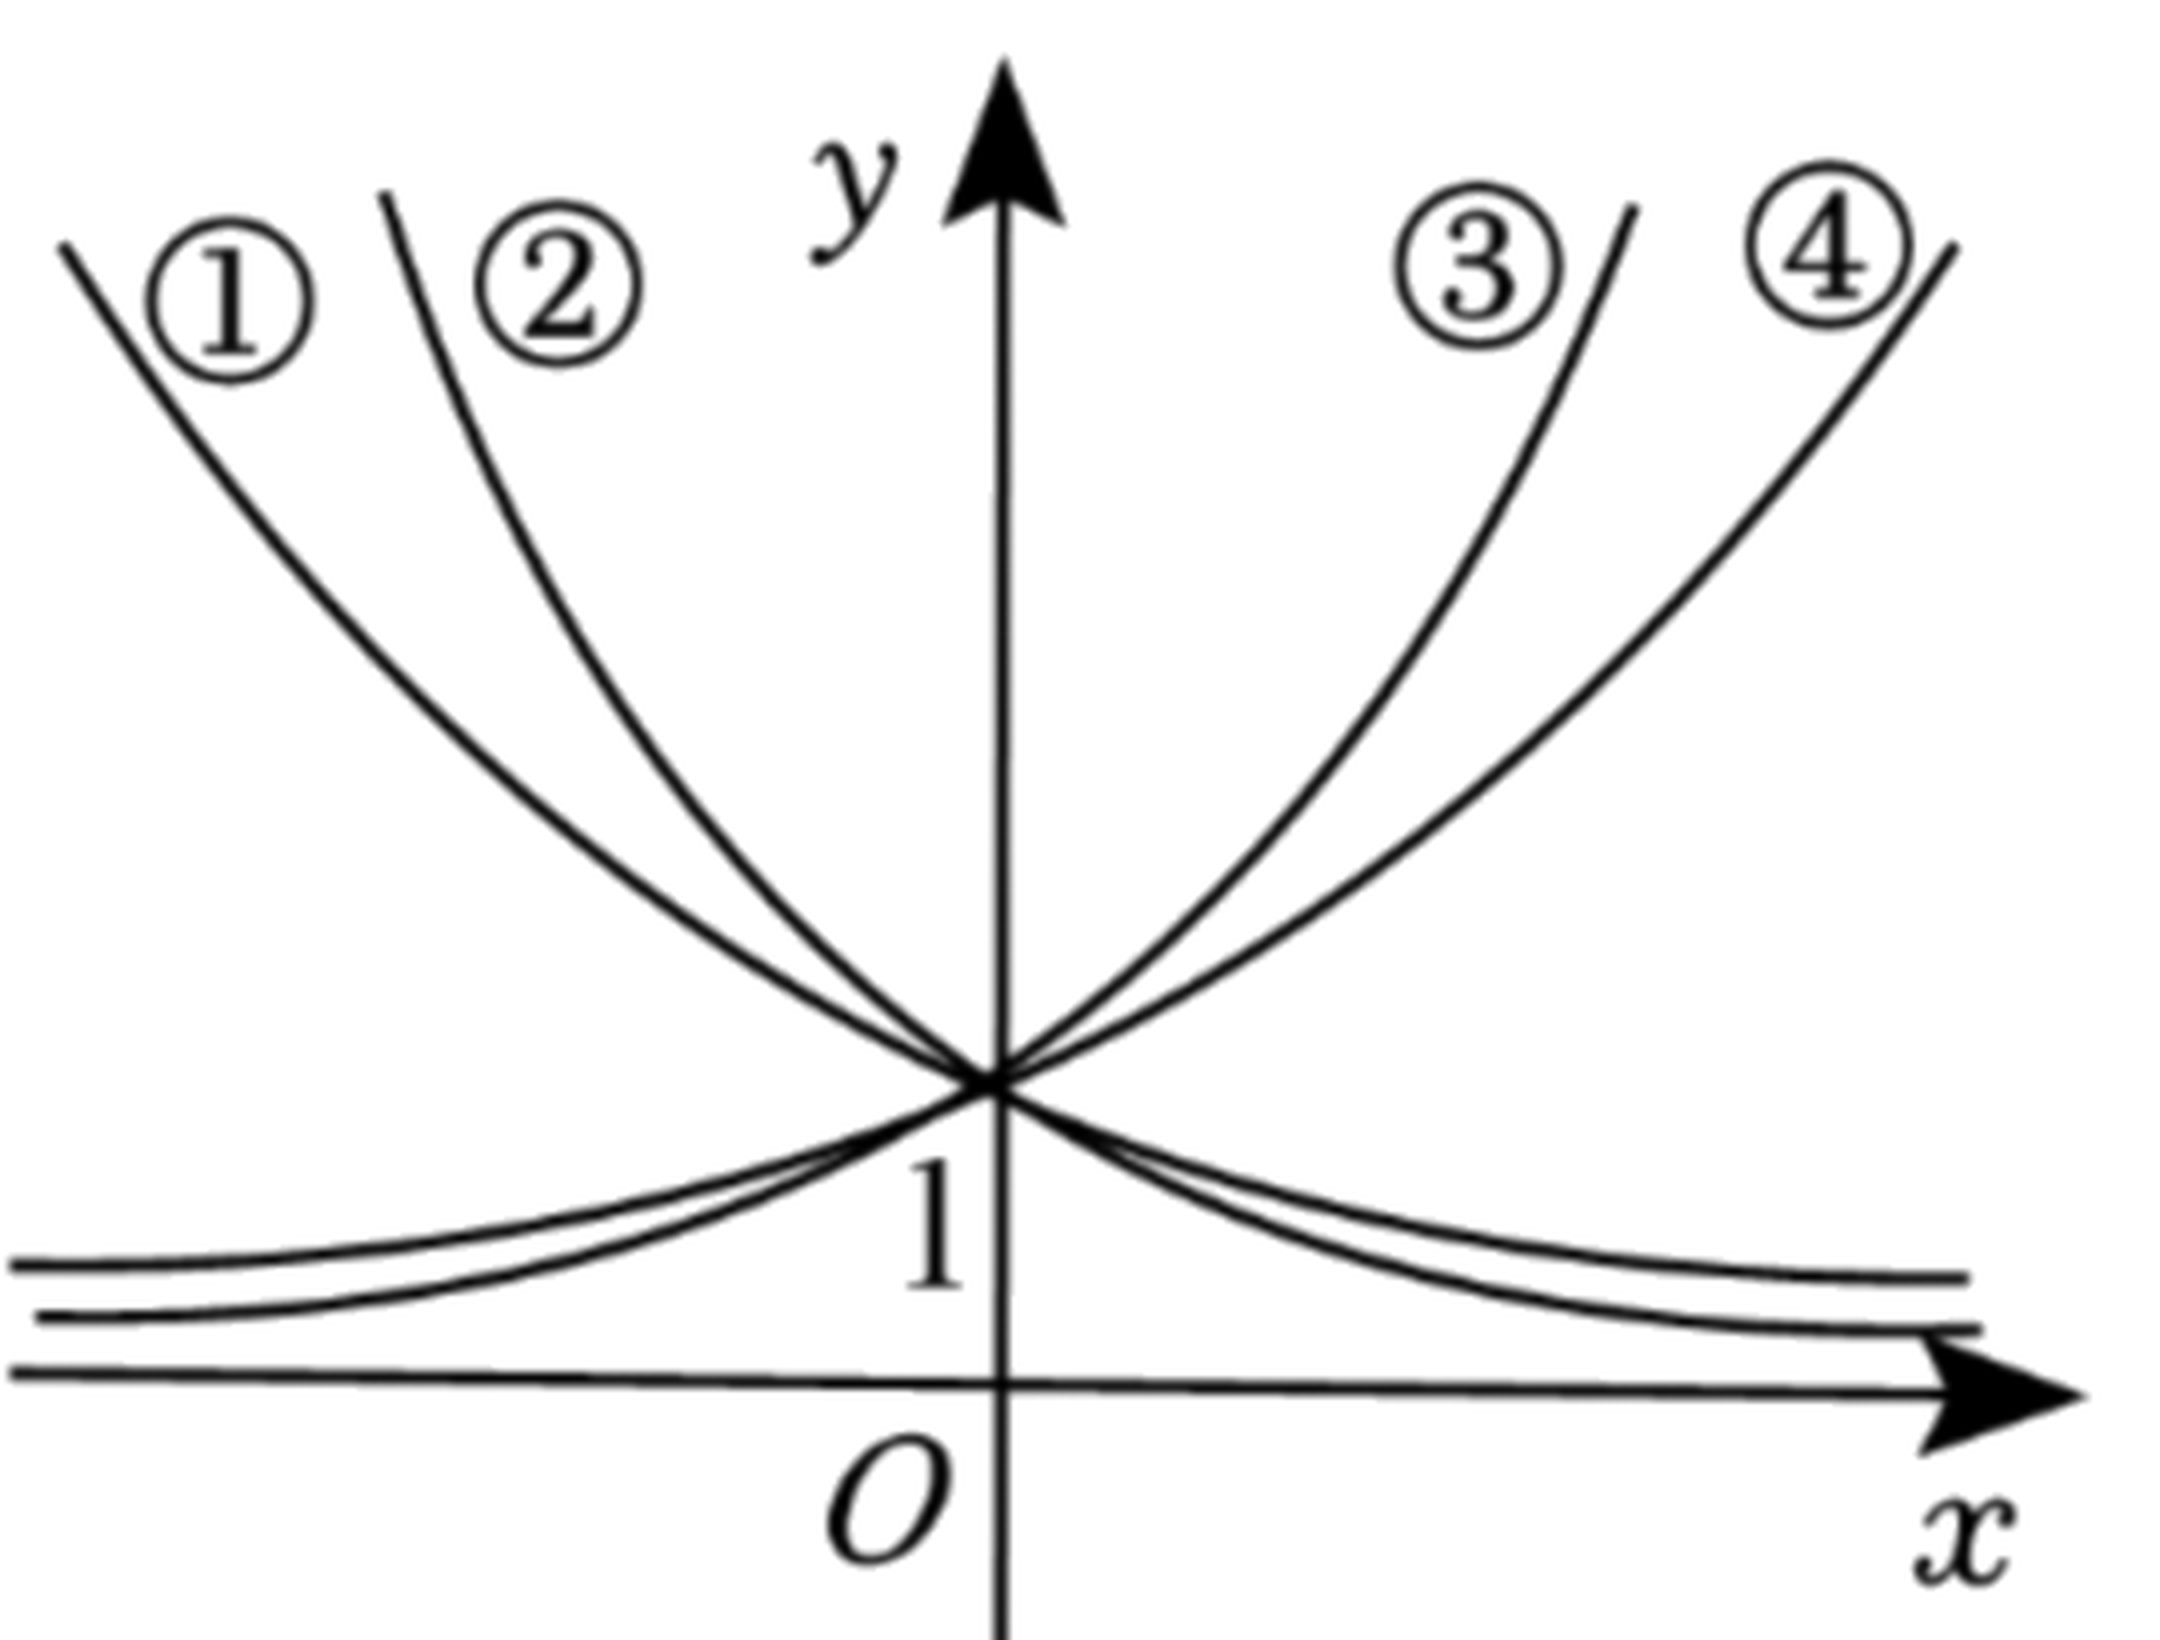
\includegraphics[width=0.40\textwidth]{figures/gao148_q15.png}
\end{center}

\ifanswer
\solbegin
\step{由函数图象得函数① $y=a^x$；② $y=b^x$ 为减函数，且 $x=1$ 时，$b^1<a^1$，}
\step{所以 $0<b<a<1$，}
\step{由函数图象得函数③ $y=c^x$；④ $y=d^x$ 为增函数，且 $x=1$ 时，$c^1>d^1$，}
\step{所以 $c>d>1$，}
\step{所以 $b<a<d<c$. 故选 $B$.}
\solend
\fi

% === Q16 ===：题目配图（关于 y 轴对称的幂函数曲线，三版都出），\needvspace 守卫放 \item 之前；$p$、$q\in\Z$；"图象"照录；解析 2 行
\needvspace{8cm}
\item 已知幂函数 $y=x^{\frac{p}{q}}$（$p$、$q\in\Z$ 且 $p$、$q$ 互质）的图象关于 $y$ 轴对称，如图所示，则\mbox{（\quad）}

\keepwithprev
A. $p$、$q$ 均为奇数，且 $\dfrac{p}{q}>0$\qquad\qquad B. $q$ 为偶数，$p$ 为奇数，且 $\dfrac{p}{q}<0$

C. $q$ 为奇数，$p$ 为偶数，且 $\dfrac{p}{q}>0$\qquad\qquad D. $q$ 为奇数，$p$ 为偶数，且 $\dfrac{p}{q}<0$

\begin{center}
% 关于 y 轴对称的幂函数曲线图取 04 页右下，去粉色水印、去色、4× LANCZOS 放大；三版都出
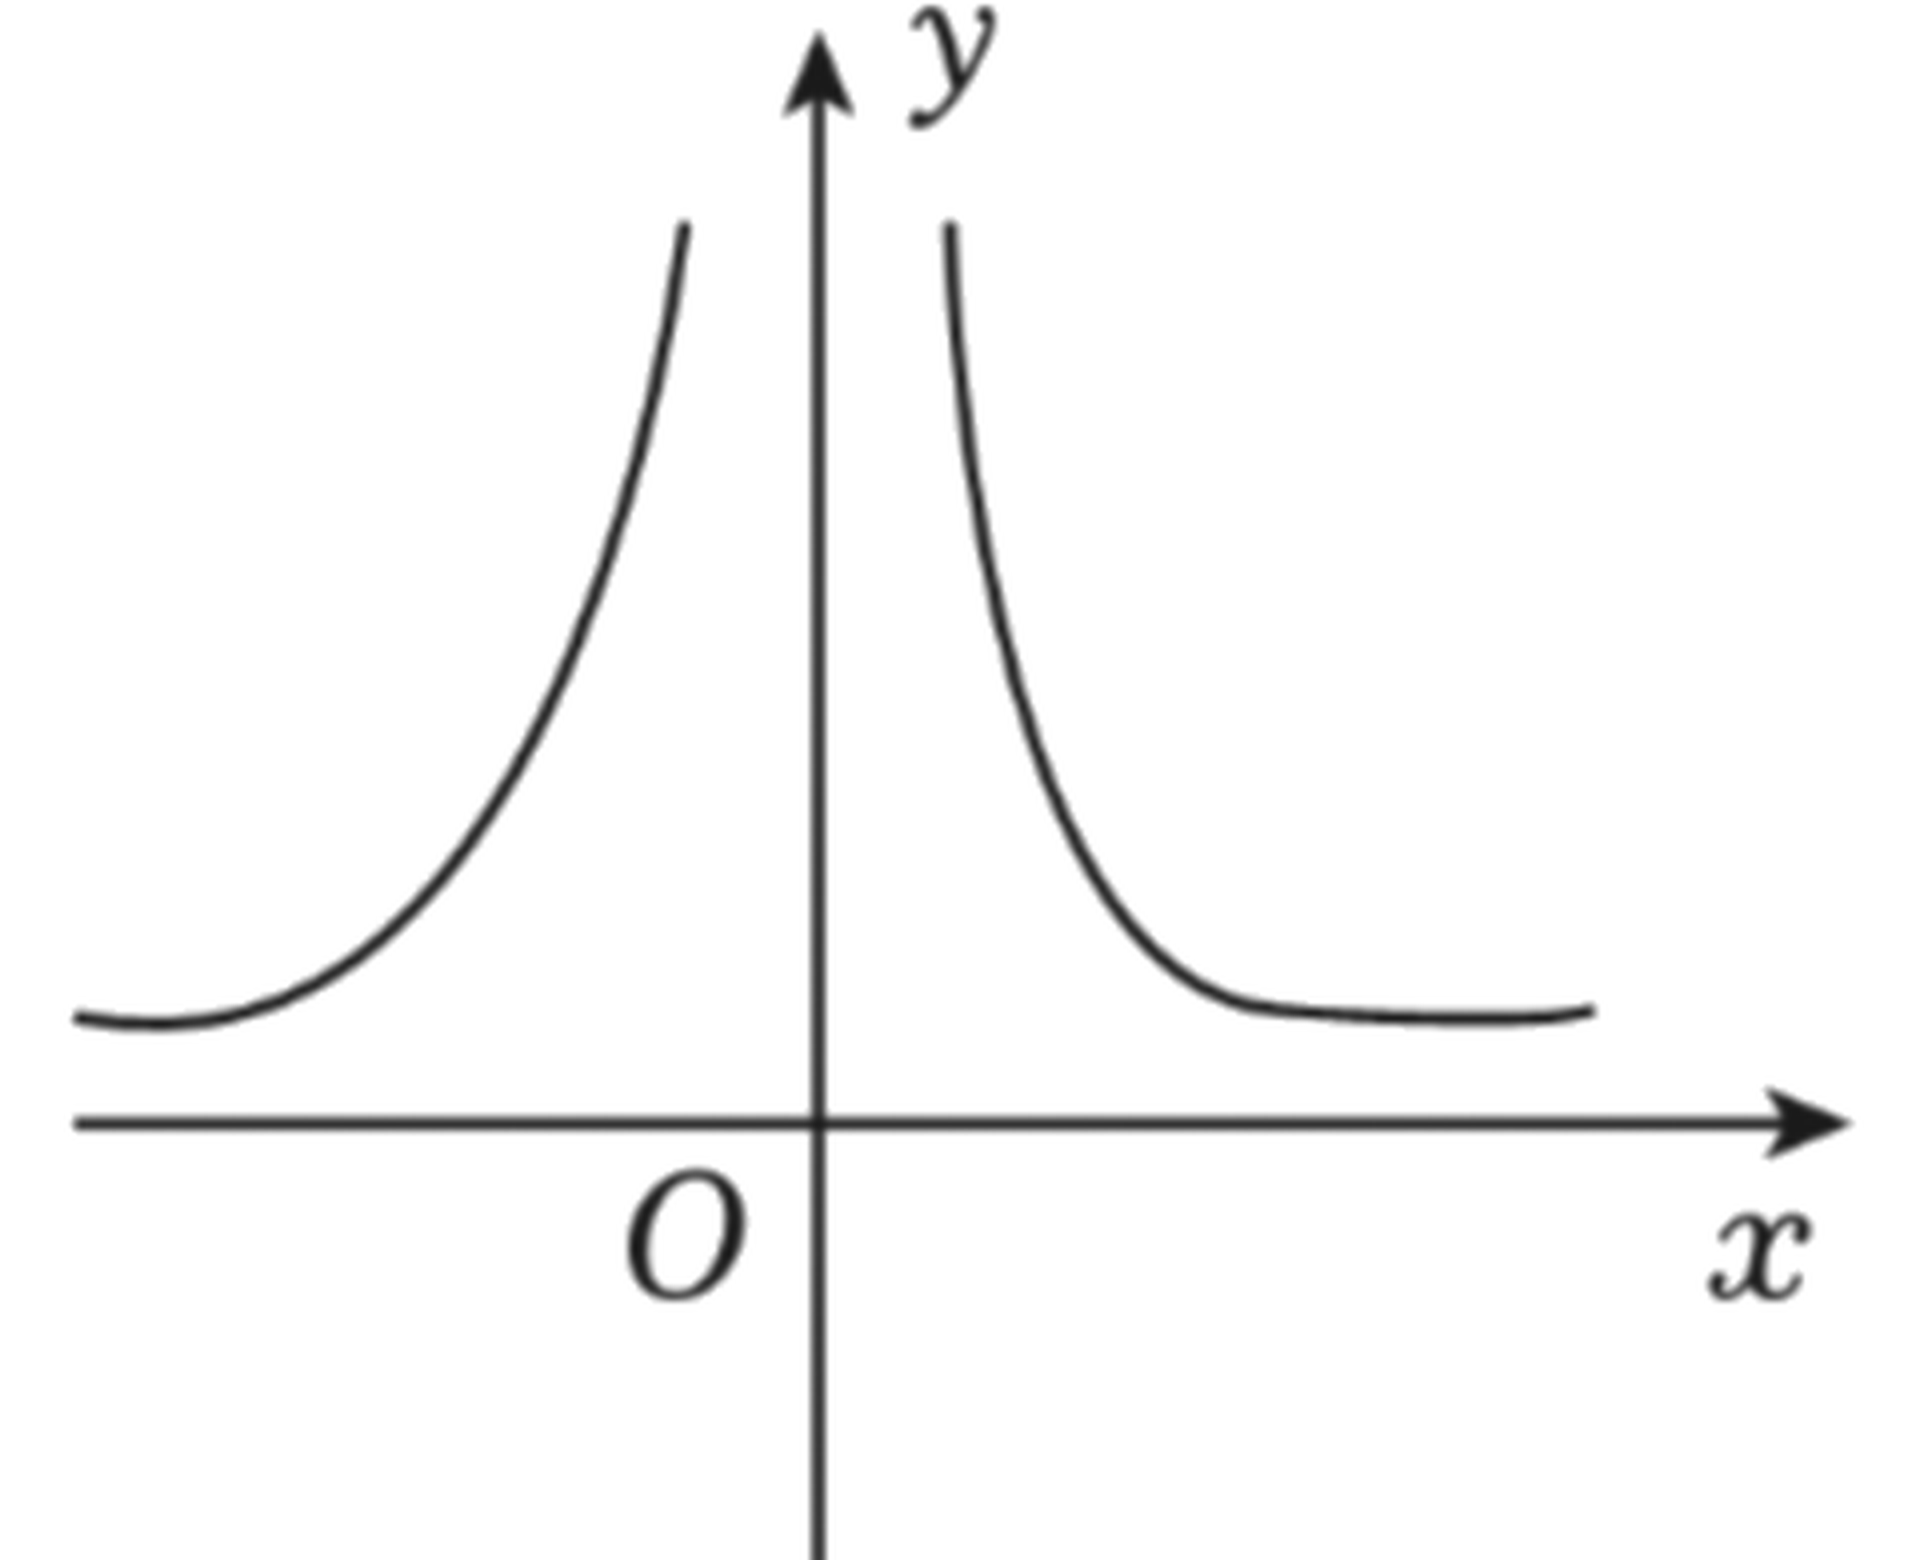
\includegraphics[width=0.36\textwidth]{figures/gao148_q16.png}
\end{center}

\ifanswer
\solbegin
\step{因为函数为偶函数，所以 $p$ 为偶数，且由图象形状判定 $\dfrac{p}{q}<0$.}
\step{又 $p$、$q$ 互质，所以 $q$ 为奇数. 故选 $D$.}
\solend
\fi

\end{enumerate}

\bigsec{三、解答题}

\begin{enumerate}
\setcounter{enumi}{16}

% === Q17 ===：\overline{B}／\varnothing／\R／\mid 逐处照录；解析 8 行
\item 已知集合 $A=\left\{x\mid \dfrac{5}{2x+1}>1\right\}$，$B=\{x\mid x^2+(a+3)x+3a<0,a\in\R\}$.

(1) 求 $A$.

(2) 若全集 $U=\R$，且 $A\cap\overline{B}=\varnothing$，求实数 $a$ 的取值范围.

\ifanswer
\solbegin
\step{(1) $\dfrac{5}{2x+1}>1$，即 $\dfrac{5}{2x+1}-1>0$，即 $\dfrac{4-2x}{2x+1}>0$，即 $(2x+1)(x-2)<0$，}
\step{解得 $-\dfrac{1}{2}<x<2$，所以 $A=\left(-\dfrac{1}{2},2\right)$；}
\step{(2) $x^2+(a+3)x+3a<0$，即 $(x+3)(x+a)<0$，}
\step{全集 $U=\R$，且 $A\cap\overline{B}=\varnothing$，}
\step{当 $a<3$ 时，解得 $-3<x<-a$，则 $\overline{B}=(-\infty,-3)\cup(-a,+\infty)$，}
\step{此时 $-a\geqslant2$，解得 $a\leqslant-2$，}
\step{当 $a\geqslant3$ 时，不满足 $A\cap\overline{B}=\varnothing$，}
\step{故实数 $a$ 的取值范围是 $(-\infty,-2]$.}
\solend
\fi

% === Q18 ===：cases 块整体算一个印刷行；解析 6 行
\item 已知幂函数经过点 $(2,4)$.

(1) 当 $x=\dfrac{1}{2}$ 时，求函数的值；

(2) 是否存在实数 $m$、$n$，使得该函数在区间 $[m,n]$ 上最小值为 $6m-8$，最大值为 $6n-8$？若存在，求出 $m$、$n$ 的值，若不存在，请说明理由.

\ifanswer
\solbegin
\step{(1) 设幂函数的解析式是 $y=x^\alpha$，则 $2^\alpha=4$，解得 $\alpha=2$，}
\step{故 $f(x)=x^2$，$f\left(\dfrac{1}{2}\right)=\dfrac{1}{4}$；}
\step{(2) 因为 $f(x)\geqslant0$，所以 $6m-8\geqslant0$，$m\geqslant\dfrac{4}{3}$，}
\step{由函数 $f(x)$ 在 $(0,+\infty)$ 严格增，得函数 $f(x)$ 在 $(m,n)$ 严格增，}
\step{所以 $\begin{cases}f(m)=6m-8\\f(n)=6n-8\end{cases}$ 且 $m<n$，解得 $m=2$，$n=4$，}
\step{故存在 $m=2$，$n=4$ 满足题意.}
\solend
\fi

% === Q19 ===：7 处评分档照 高一54／64 成例排 \dots\dots N 分；判别式高 \Delta；解析 9 行
\item 已知方程 $x^2+6mx+9m-2=0$，且 $x_1,x_2$ 是方程的两个不同的实数根.

(1) 若 $m=1$，求 $\dfrac{1}{x_1}+\dfrac{1}{x_2}$ 的值；

(2) 若 $m\in\R$，且 $x_1^2+x_2^2<4$，求 $m$ 取值范围.

\ifanswer
\solbegin
\step{(1) 当 $m=1$ 时，方程为 $x^2+6x+7=0$，\dots\dots1 分}
\step{则 $x_1+x_2=-6,x_1\cdot x_2=7$，\dots\dots2 分}
\step{$\dfrac{1}{x_1}+\dfrac{1}{x_2}=\dfrac{x_1+x_2}{x_1\cdot x_2}=-\dfrac{6}{7}$\dots\dots3 分}
\step{(2) $x_1+x_2=-6m,x_1\cdot x_2=9m-2$\dots\dots2 分}
\step{因为 $x_1^2+x_2^2=(x_1+x_2)^2-2x_1\cdot x_2$，所以 $(x_1+x_2)^2-2x_1\cdot x_2<4$，}
\step{所以 $36m^2-2(9m-2)<4$，解得 $0<m<\dfrac{1}{2}$\dots\dots2 分}
\step{又因为方程有两个不同的根，所以 $\Delta=36m^2-4(9m-2)>0$，}% 判别式原卷印等腰偏高粗三角 $\Delta$，照录（放大 07 页 q19_delta3.png／diag_band_q19.png 确认）
\step{解得 $m<\dfrac{1}{3}$ 或 $m>\dfrac{2}{3}$\dots\dots2 分}
\step{所以 $0<m<\dfrac{1}{3}$\dots\dots2 分}
\solend
\fi

% === Q20 ===：题目配图（矩形蔬菜温室，三版都出），\needvspace 守卫放 \item 之前；单位 \mathrm{m}／\mathrm{m}^2；解析 10 行
\needvspace{8cm}
\item 某村计划建造一个室内面积为 $600\mathrm{m}^2$ 的矩形蔬菜温室，在室内，沿左、右两侧与后侧内墙各保留 $2\mathrm{m}$ 宽的通道，沿前侧内墙保留 $4\mathrm{m}$ 宽的空地.

\begin{center}
% 矩形蔬菜温室示意图取 07 页右侧，去粉色水印、去色、4× LANCZOS 放大；三版都出
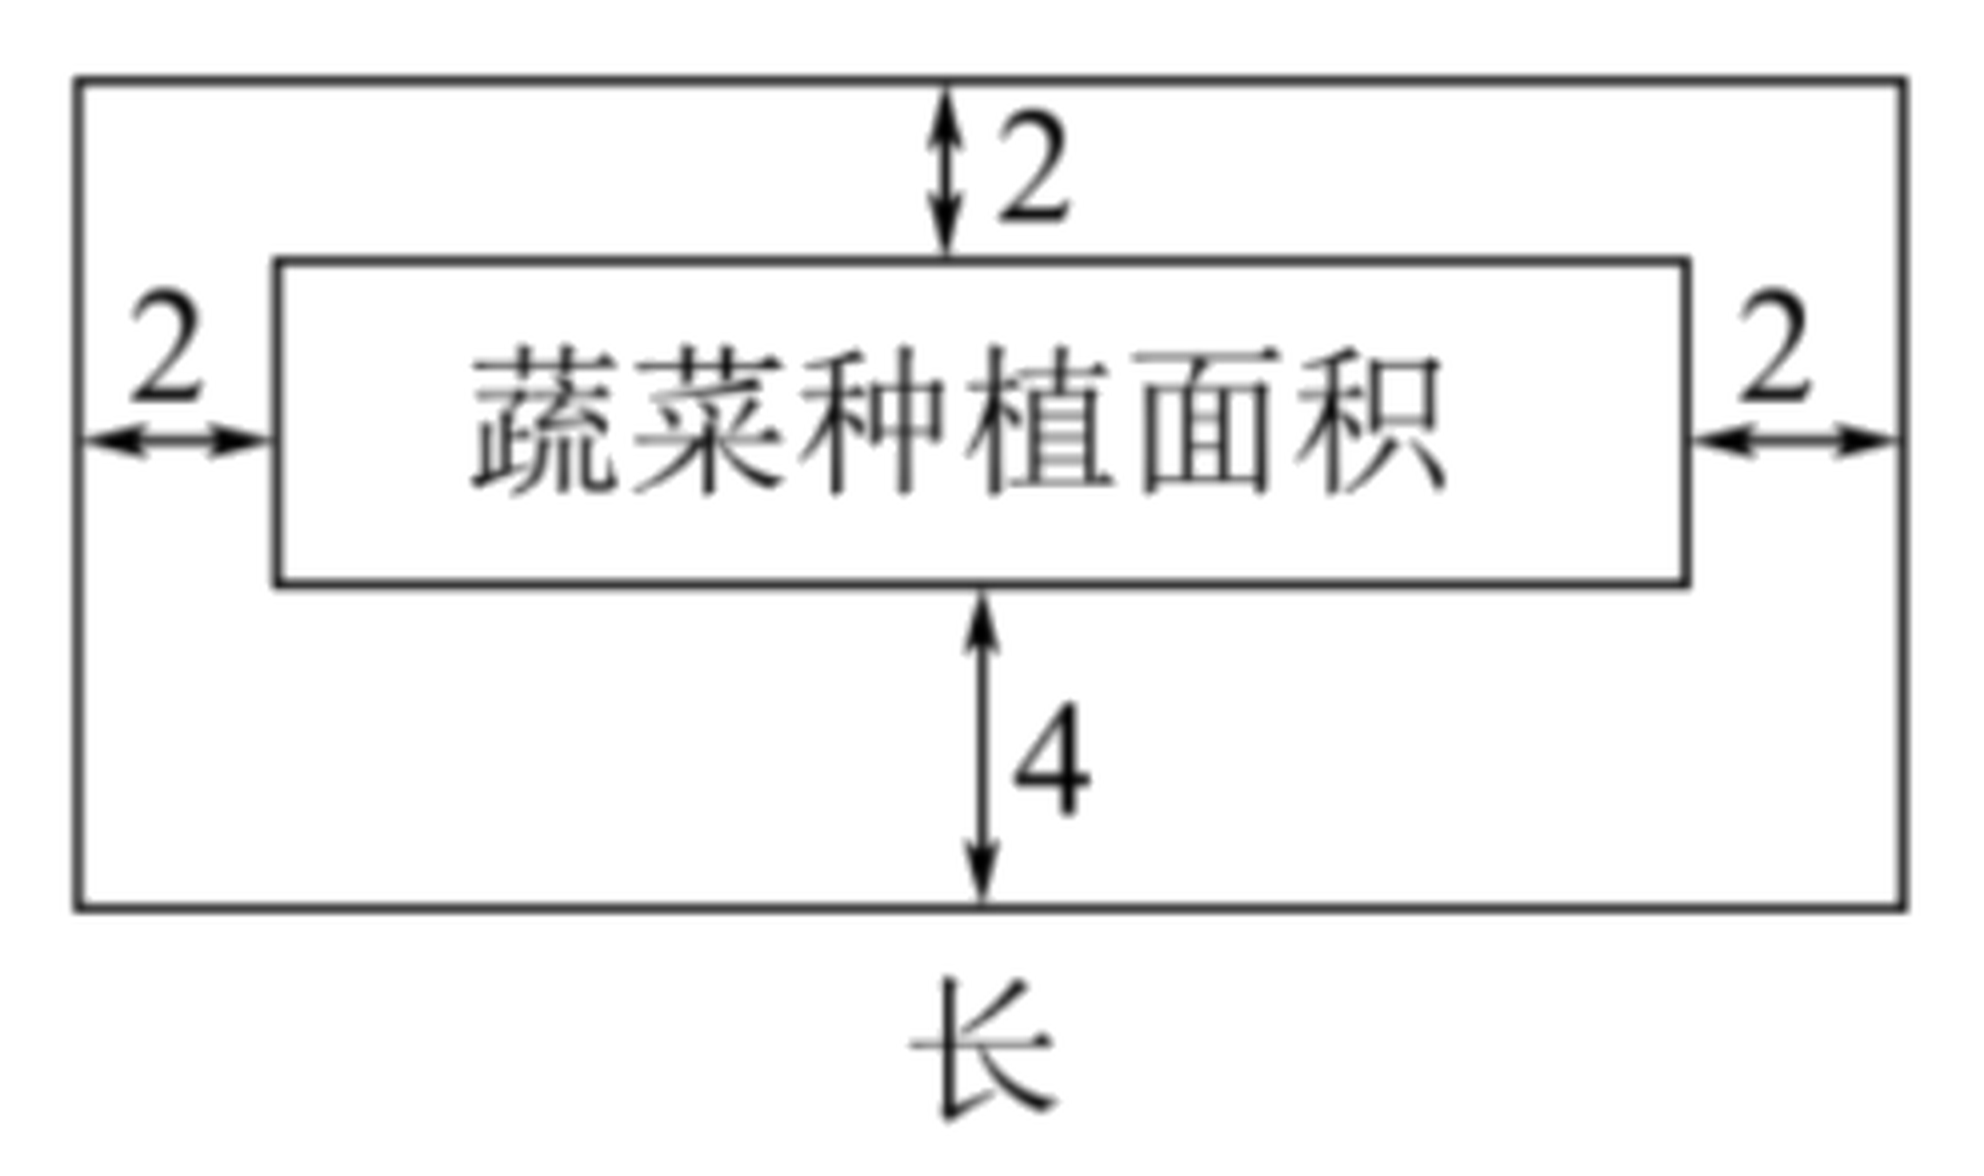
\includegraphics[width=0.45\textwidth]{figures/gao148_q20.png}
\end{center}

(1) 写出蔬菜的种植面积关于矩形温室的长之间的关系式.

(2) 当矩形温室的边长各为多少时，蔬菜的种植面积最大？最大种植面积是多少？

\ifanswer
\solbegin
\step{(1) 设蔬菜的种植面积为 $y\mathrm{m}^2$，矩形温室的长为 $x\mathrm{m}$，}
\step{则矩形温室的宽为 $\dfrac{600}{x}\mathrm{m}$，}
\step{种植蔬菜矩形的长为 $(x-4)\mathrm{m}$，宽为 $\left(\dfrac{600}{x}-6\right)\mathrm{m}$，}
\step{所以 $y=(x-4)\left(\dfrac{600}{x}-6\right)(4<x<100)$；}
\step{(2) 因为 $y=(x-4)\left(\dfrac{600}{x}-6\right)=624-\left(6x+\dfrac{2400}{x}\right)$，}
\step{因为 $6x+\dfrac{2400}{x}\geqslant2\sqrt{6x\cdot\dfrac{2400}{x}}=240$，}
\step{当且仅当 $6x=\dfrac{2400}{x}$，即 $x=20$ 时取等号，}
\step{所以 $y=624-\left(6x+\dfrac{2400}{x}\right)\leqslant624-240=384$.}
\step{即当矩形温室的一边长为 $20\mathrm{m}$，另一边长为 $30\mathrm{m}$ 时，}
\step{蔬菜的种植面积最大，最大为 $384\mathrm{m}^2$.}
\solend
\fi

% === Q21 ===：3 问、cases 块整体算一个印刷行；判别式高 \Delta；解析 19 行（末行续 09 页）
\item 二次函数 $f(x)=ax^2+bx+c$ 满足对任意的 $x\in\R$，$x-1\leqslant f(x)\leqslant x^2-x$ 恒成立.

(1) 求证：$f(1)$ 为定值；

(2) 若 $f(0)=-\dfrac{1}{4}$，求二次函数 $f(x)$ 的表达式；

(3) 求 $a+2b+5c$ 的取值范围.

\ifanswer
\solbegin
\step{(1) 对任意的 $x\in\R$，$x-1\leqslant f(x)\leqslant x^2-x$ 恒成立，则 $0\leqslant f(1)\leqslant0$，}
\step{所以 $f(1)=0$，为定值.}
\step{(2) 由(1)得 $a+b+c=f(1)=0$，由 $f(0)=-\dfrac{1}{4}$，得 $c=-\dfrac{1}{4}$，}
\step{则 $b=\dfrac{1}{4}-a$，$f(x)=ax^2+\left(\dfrac{1}{4}-a\right)x-\dfrac{1}{4}$，}
\step{不等式 $x-1\leqslant f(x)$ 可化为 $ax^2+\left(\dfrac{1}{4}-a\right)x-\dfrac{1}{4}\geqslant x-1$，}
\step{即 $ax^2-\left(a+\dfrac{3}{4}\right)x+\dfrac{3}{4}\geqslant0$，}
\step{一元二次不等式 $ax^2-\left(\dfrac{3}{4}+a\right)x+\dfrac{3}{4}\geqslant0$ 恒成立，则 $\begin{cases}a>0\\\Delta=\left(a+\dfrac{3}{4}\right)^2-3a\leqslant0\end{cases}$，}% 判别式原卷印等腰偏高粗三角 $\Delta$，照录（放大 08 页 q21_delta3.png／diag_band_q21.png 确认）
\step{解得 $a=\dfrac{3}{4}$，}
\step{此时 $f(x)=\dfrac{3}{4}x^2-\dfrac{1}{2}x-\dfrac{1}{4}$，$x^2-x-f(x)=\dfrac{1}{4}(x-1)^2\geqslant0$ 恒成立，}
\step{所以 $f(x)=\dfrac{3}{4}x^2-\dfrac{1}{2}x-\dfrac{1}{4}$.}
\step{(3) 由(1)得 $b=-a-c$，$f(x)=ax^2-(a+c)x+c=(ax-c)(x-1)$，}
\step{不等式 $x-1\leqslant f(x)$ 可化为 $(x-1)(ax-c-1)\geqslant0$，}
\step{一元二次不等式 $(x-1)(ax-c-1)\geqslant0$ 恒成立，则 $a>0$，}
\step{且方程 $(x-1)(ax-c-1)=0$ 有相等的实数根，因此 $c=a-1$，$a>0$，}
\step{不等式 $f(x)\leqslant x^2-x\Leftrightarrow(ax-c)(x-1)\leqslant x^2-x\Leftrightarrow(x-1)[(1-a)x+c]\geqslant0$，}
\step{同理 $1-a>0$，且方程 $(x-1)[(1-a)x+c]=0$ 有相等的实数根，}
\step{因此 $c=a-1$，$a<1$，从而 $c=a-1$，$b=1-2a$，$0<a<1$，}
\step{$a+2b+5c=a+2(1-2a)+5(a-1)=2a-3\in(-3,-1)$，}
\step{所以 $a+2b+5c$ 的取值范围是 $(-3,-1)$.}
\solend
\fi

\end{enumerate}

\end{document}
"
%
% ① 原始材料：微信公众号"魔都数学加油站"文章，连载"27学年高一148"，原文标题
% "27学年高一148——2026-2027年上海市新川中学高一上期中"（2026-11-21 推送）；
% 原文链接：https://mp.weixin.qq.com/s/Alhmwb3sSLQMp_wjzoAVyA 。
% 正文为 9 张 PNG 页（01/03/04/07/08/09 为 2560×3620，02/05/06 为 4762×6735，
% 同一篇各页分辨率混排，逐页按各自分辨率裁图核对，别按预览比例换算裁框）。
% 体例：混合体例讲评版——19 题中 Q4、Q5 只印【答案】、无【解析】；Q13 的答案"C"
% 直接印在题干括号内、无【答案】/【解析】段；其余 16 题印【解析】（逐题核实，见 ② ②）。
% 题目、答案、解析均据原图转录；卷面粉红色水印"魔都数学加油站"及公众号页脚未录入。
% 全卷插图清单（逐页通读 9 页确认）：4 幅题目配图，均三版都出、均非【解析】内配图：
%   · Q12 幂函数曲线族图（03 页右侧：x/y 轴、O、A(1,0)、B(0,1)、M、N 与两族
%     y=x^α／y=x^β 曲线、线段 AB、虚线），题干"（如图）"处，裁 figures/gao148_q12.png；
%   · Q15 四条指数函数曲线图（04 页右侧：①②③④ 四曲线同过 (0,1)、x/y 轴、O、
%     y 轴刻度 1），题干"如图"处，裁 figures/gao148_q15.png；
%   · Q16 关于 y 轴对称的幂函数曲线图（04 页右下：x/y 轴、O、两支上翘曲线），
%     题干"如图所示"处，裁 figures/gao148_q16.png；
%   · Q20 矩形蔬菜温室示意图（07 页右侧：大矩形＋内框"蔬菜种植面积"＋2/2/4
%     通道标注＋"长"），题干处，裁 figures/gao148_q20.png；
%   其余各页逐页确认无其它题目配图、无【解析】内配图、无表格，亦无"题干写如图而
%   源码漏图"一处；Q19 解析行末的虚线"----N 分"为评分档（非图），Q18／Q21 的
%   cases 块为数学块（非图）。4 图均取自原卷截图，去粉色水印、去色、4× LANCZOS 放大。
%
% 卷首标题：原卷印作"2026-2027 年新川中学高一上期中"，年份区间按全稿惯例排 en dash；
% 原卷卷面未印副标题，本稿按同期中卷（高一140／141／143／144／145／146／147）知识模块
% 口径补出"集合与常用逻辑用语、不等式、函数"。
%
% 题号体例（逐页核实定稿）：本卷共 19 题——一、填空题 3—12（10 题）、
% 二、选择题 13—16（4 题）、三、解答题 17—21（5 题）。
% 三节分别 \setcounter{enumi}{2}／{12}／{16}。原卷从第 3 题起、无第 1、2 题，
% 本稿保留原题号；全卷无附加题节、无 Q22（Q21 解析末行"所以 a+2b+5c 的取值范围是
% (-3,-1)."为全卷收尾，09 页下半仅水印、无正文）。
%
% ② 与原卷的排版差异：
%   ① 原文从第 3 题起，本稿保留原题号；共 19 题三节；
%   ② 混合体例逐题核实：Q4（反证法"假设的内容"）、Q5 只印【答案】、无【解析】，
%      按 高一140 第 5 题／高一145 Q3 成例提 \ans{}、不补造解析；Q13 答案"C"直接
%      印在题干括号内（" ( C ) "）、全卷无该题【答案】/【解析】段，按 高一84 Q13／
%      高一37 Q13／高一53 Q13 成例括号 \mbox{（\quad）} 留空、另提 \ans{$C$}；
%      其余 16 题印【解析】、用 \solbegin…\solend，选择题答案在解析末句"故选 X"
%      （Q14 选 D、Q15 选 B、Q16 选 D，逐个放大原图核实）、题干括号留空、不另提
%      \ans{}；答案版【答案】/【解析】标记数 = 19（3 个 \ans ＋ 16 个 \solbegin）
%      = 全卷题数；
%   ③ 原卷卷面未印副标题，本稿按知识模块口径补出；
%   ④ 原卷填空横线按全稿惯例排 \blankline[4.4em]；选择题括号排 \mbox{（\quad）}、
%      选项段前按惯例加 \keepwithprev；Q13／Q16 四选项为两行两列、Q14／Q15 选项
%      为一行，照原卷分行；解答题不留作答区、不加 \anspace（原卷为讲评版，
%      与 129／131／132／133／136／140／141／143／144／145／146 同）；
%   ⑤ 数集：Q11"在 R 上定义运算"、Q13"x、y∈R"、Q16"p、q∈Z"、Q17"a∈R"
%      "U=R"、Q19"m∈R"、Q21"x∈R" 原卷印斜体 R/Z，按全稿惯例统一改 \R／\Z
%      （本卷未出现 N，\N^* 无对应处）；绝对值排 \lvert…\rvert（Q9／Q14），
%      集合描述竖线排 \mid（Q17）；不等号按全稿惯例排 \leqslant／\geqslant；
%      补集照原卷上划线排 \overline{B}（Q17 题干 1 处＋解析 3 处）；空集
%      \varnothing（Q17 题干 1 处＋解析 2 处）；\subset（Q3 题干 {a}⊂M）与
%      \subseteq（Q3 题干 M⊆{a,b,c,d}）逐处照录不统一（放大 01 页 q3_subset.png）；
%   ⑥ 子题标号 (1)(2)(3) 半角括号照录；圈数字 ①—⑥ 在文本模式（Q14 六个结论、
%      Q15 曲线编号与其解析、Q14 解析"对①…对⑥"），按 common.sty 划入 CJK 字符类
%      渲染；cases 块整体算一个印刷行；\left…\right 不得拆到不同 $…$ 组；
%      单位 m／m² 排 \mathrm{m}／\mathrm{m}^2（Q20，原卷印正体 m）；
%   ⑦ 题干／解析中的中文弯引号按原卷照录：Q4" ab 可以被 5 整除，那么 a、b 中
%      至少有一个能被 5 整除 "（开引号后有空格、闭引号后空格接"时"）、
%      Q13" x=0 "" xy=0 "（引号内空格），注释内一律 ASCII 引号；
%   ⑧ 半角逗号在数学组之间是全稿惯例、非笔误（Q3"{a,b,c,d}"、Q6"$x,y$"
%      "$x=\frac13,y=\frac16$"、Q10、Q11"$a=-2,b=-1"、Q12"$\alpha=\log..,\beta=..$"、
%      Q14"$a+b<0,a-b<0$"、Q17、Q19"$x_1+x_2=-6,x_1\cdot x_2=7$"、Q20、Q21 等），
%      逐处照录别改全角；行末西文句点照录为 ASCII `.`；行中全角逗号／顿号照录；
%   ⑨ "图像／图象"逐处放大核：全卷 9 处均印"图象"（象，无亻）、未见"图像"，
%      逐处照录未统一改动（Q8 题干/解析各 1、Q12 题干 2、Q15 题干 1／解析 2、
%      Q16 题干 1／解析 1；放大 02/03/04/05 页 /tmp/gao148/zoom/my_wide_a.png、
%      my_wide_b.png 与宋体参考"象／像"并排确认）；
%   ⑩ 判别式 Δ/△ 混用是照录项：Q11 解析"△=1−4(−a²+a+1)<0"印扁等边空心
%      三角 \triangle；Q19 解析"Δ=36m²−4(9m−2)>0"、Q21 解析 cases 块
%      "Δ=(a+3/4)²−3a≤0" 两处印等腰偏高粗三角 \Delta，逐处放大判断、照录
%      不统一（参照 高一142／144／145 头注④口径，详见 ④）；
%   ⑪ 一条 \step = 原卷解析的一个印刷行，cases 块整体算一个印刷行；别把原卷折行
%      并起来、别把一行拆多条。Q3 六行、Q7 五行（01 页末首行＋02 页顶四行）、
%      Q9 七行、Q11 五行、Q14 八行（对② 的两行公式各占一印刷行）、Q17 八行、
%      Q18 六行、Q19 九行（7 处评分档附在行末）、Q20 十行、Q21 十九行
%      均按印刷行逐条断，不丢行；
%   ⑫ 配图：4 幅均为题目配图（三版都出），放 \item 内题干之后 \begin{center}；
%      大图块加 \needvspace 守卫把整块推走（守卫放 \item 之前，见 高一145 Q14/Q20
%      成例与切页审计 B 类坑）；三版切页审计均"合计异常：无"；
%   ⑬ 跨页续印按题合并：Q3/4/5 在 01 页；Q6 题干＋解析在 01 页；Q7 题干在 01 页
%      末、解析首行在 01 页末续 02 页顶四行；Q8/9/10 在 02 页（Q9 解析续 02 页下半、
%      Q10 题干与解析前 2 行在 02 页末）；Q10 解析末行续 03 页顶；Q11/12 在 03 页、
%      "二、选择题"标题与 Q13/14 题干在 03 页下半；Q13 无解析；Q14 解析在 04 页顶、
%      Q15 题干＋图＋选项＋解析在 04 页、Q16 题干＋图在 04 页末；Q16 选项＋解析＋
%      "三、解答题"标题＋Q17 题干＋解析在 05 页、Q18 题干首句在 05 页末；Q18 题干
%      续＋解析、Q19 题干＋解析前 5 行在 06 页；Q19 解析续 4 行＋Q20 题干＋图＋
%      解析（10 行全部）在 07 页，末行"蔬菜的种植面积最大，最大为 384m²."收尾；
%      Q21 题干＋解析前 18 行在 08 页；Q21 解析末行"所以 a+2b+5c 的取值范围是
%      (-3,-1)."在 09 页上半（09 页下半仅水印、无正文）。本稿按题连排，不丢行、
%      不并折行；
%   ⑭ 原卷解析内无红色"法一／法二"之类小标题，故本卷无 \stepm；水印
%      "魔都数学加油站"红色不录入；Q19 解析 7 处评分档（1/2/3/2/2/2/2 分）
%      原卷在行末印一串虚线，本稿照 高一54／64 成例排 \dots\dots N 分，
%      分值逐处照录、位置不变。
%
% ③ 行数复核：一条 \step／\stepm = 原卷解析的一个印刷行，cases 块作一个印刷行计。
%   逐题数（主会话逐页核对定稿）：Q3：6；Q4：0（只印【答案】、提 \ans{}）；
%   Q5：0（只印【答案】、提 \ans{}）；Q6：2；Q7：5；Q8：2；Q9：7；Q10：3；
%   Q11：5；Q12：2；Q13：0（答案印在题干括号内、另提 \ans{}）；Q14：8；Q15：5；
%   Q16：2；Q17：8；Q18：6；Q19：9；Q20：10；Q21：19。
%   合计 99 条 \step（本卷无 \stepm：解析内无红色"法一／法二"类小标题），
%   与原卷逐题印刷行相等。全卷 16 题设 \solbegin…\solend ＋ 3 处 \ans{}，
%   答案版【答案】/【解析】标记数 = 19 = 全卷题数。
%
% ④ 判别式／子集符号结论（逐处放大原图照录、不得统一，主会话像素级复核）：
%   判别式全卷 3 处，两形混用逐处照录不统一（参照 高一142／144／145 头注④口径）：
%     · Q11 解析"△=1−4(−a²+a+1)<0" 原卷印扁等边空心三角（宽>高、细线），
%       照录 \triangle（放大 03 页 /tmp/gao148/zoom/q11_delta3.png、
%       delta_montage.png 确认）；
%     · Q19 解析"Δ=36m²−4(9m−2)>0" 原卷印等腰偏高粗三角（高>宽），
%       照录 \Delta（放大 07 页 /tmp/gao148/zoom/q19_delta3.png 确认）；
%     · Q21 解析 cases 块"Δ=(a+3/4)²−3a≤0" 原卷印等腰偏高粗三角（高>宽），
%       照录 \Delta（放大 08 页 /tmp/gao148/zoom/q21_delta3.png 确认）。
%   子集／补集：Q3 题干"{a}⊂M⊆{a,b,c,d}" 前者印单线 ⊂、无下划线，照录 \subset；
%     后者印带下划线 ⊆，照录 \subseteq（放大 01 页 /tmp/gao148/zoom/q3_subset.png
%     确认）；Q17 题干 1 处＋解析 3 处共 4 处 \overline{B} 照原卷上划线
%     （B 上横线、非 C_U B）；空集 \varnothing 3 处（Q17 题干 1 处、解析 2 处）；
%     Q17 集合描述竖线 \mid；数集 \R／\Z 归一见 ② ⑤。
%
% ⑤ 存疑照录（放大原图确认，照录未改、正文对应处另有 % 注）：
%   1. Q3 解析末行"所以 M 一共有 3+3+1+1=8 个" 原卷印 $3+3+1+1=8$，按上文
%      四行应为 $1+3+3+1=8$（疑为原卷加数顺序笔误，和仍为 8），放大 01 页
%      /tmp/gao148/zoom/my_q3_sol.png 确认，照录未改。
%   2. Q13 答案"C"直接印在题干括号内、全卷无该题【答案】/【解析】段，按
%      高一84 Q13 成例括号留空、另提 \ans{$C$}（见 ② ②），未补造解析。
%   3. Q19 解析 7 处评分档（"----N 分"）原卷印一串虚线，本稿照 高一54／64
%      成例排 \dots\dots N 分，分值逐处照录、位置不变。
%   4. 判别式 Q11 扁 \triangle 与 Q19／Q21 高 \Delta 两形混用，逐处照录不统一（见 ④）。
%   5. "图像／图象"全卷 9 处均印"图象"、未见"图像"（见 ② ⑨），逐处放大核实照录，
%      未统一改动。
%   全卷除此 5 类外未发现其它笔误／自相矛盾处。
%
% ⑥ 跨页续印按题合并说明：见 ② ⑬。
%
\documentclass[a4paper,11pt]{article}
\usepackage{common}

\begin{document}

\examtitlest[3]{2026--2027 年新川中学高一上期中}{集合与常用逻辑用语、不等式、函数}

\bigsec{一、填空题}

\begin{enumerate}
\setcounter{enumi}{2}

% === Q3 ===：题干 {a}⊂M⊆{a,b,c,d} 两个子集符号逐处照录；解析 6 行
\item 满足 $\{a\}\subset M\subseteq\{a,b,c,d\}$ 的集合 $M$ 有\blankline[4.4em]个.

\ifanswer
\solbegin
\step{$M$ 是 $\{a,b,c,d\}$ 的子集，但必含有元素 $a$，}
\step{当 $M$ 中只一个元素时，$M=\{a\}$ 只有 1 个；}
\step{当 $M$ 中有二个元素时，$M$ 有 3 个；}
\step{当 $M$ 中有三个元素时，$M$ 有 3 个；}
\step{当 $M$ 中有四个元素时，$M$ 有 1 个；}
\step{所以 $M$ 一共有 $3+3+1+1=8$ 个.}% 原卷印 $3+3+1+1=8$（按上文四行应为 $1+3+3+1$），疑为加数顺序笔误，照录未改（放大 01 页 my_q3_sol.png）
\solend
\fi

% === Q4 ===：原卷只印【答案】、无【解析】，按 高一140 第 5 题成例提 \ans{}；弯引号与空格照录
\item 用反证法证明命题 “ $ab$ 可以被 5 整除，那么 $a$、$b$ 中至少有一个能被 5 整除” 时假设的内容应该是\blankline[4.4em].

\ifanswer
\ans{$a$、$b$ 都不能被 5 整除}
\fi

% === Q5 ===：原卷只印【答案】 $[-2,1)$、无【解析】，提 \ans{}
\item 不等式 $\dfrac{x+2}{x-1}\leqslant0$ 的解集为\blankline[4.4em].

\ifanswer
\ans{$[-2,1)$}
\fi

% === Q6 ===：解析 2 行；半角逗号在数学组之间照录
\item 设 $x,y\in(0,+\infty)$，且 $x+4y=1$，则 $\dfrac{1}{x}+\dfrac{1}{y}$ 的最小值为\blankline[4.4em].

\ifanswer
\solbegin
\step{因为 $\dfrac{1}{x}+\dfrac{1}{y}=(x+4y)\left(\dfrac{1}{x}+\dfrac{1}{y}\right)=5+\dfrac{4y}{x}+\dfrac{x}{y}\geqslant5+2\sqrt{\dfrac{4y}{x}\cdot\dfrac{x}{y}}=9$，}
\step{当且仅当 $\dfrac{4y}{x}=\dfrac{x}{y}$，即 $x=2y$，即 $x=\dfrac{1}{3},y=\dfrac{1}{6}$ 时取等号，故最小值为 9.}
\solend
\fi

% === Q7 ===：题干在 01 页末、解析首行在 01 页末续 02 页顶四行；解析 5 行
\item 若不等式 $x^2+ax+b<0$ 的解集为 $(-3,-1)$，则不等式 $bx^2+ax+1\leqslant0$ 的解集为\blankline[4.4em].

\ifanswer
\solbegin
\step{不等式 $x^2+ax+b<0$ 的解集为 $(-3,-1)$，}
\step{所以方程 $x^2+ax+b=0$ 的两个实数根为 $-3$ 和 $-1$，}
\step{由根与系数的关系得 $a=4$，$b=3$，}
\step{故 $bx^2+ax+1\leqslant0$ 可化为 $3x^2+4x+1\leqslant0$，解得 $-1\leqslant x\leqslant-\dfrac{1}{3}$，}
\step{所求不等式 $bx^2+ax+1\leqslant0$ 的解集为 $\left[-1,-\dfrac{1}{3}\right]$.}
\solend
\fi

% === Q8 ===："图象"照录；解析 2 行
\item 函数 $y=a^{x-2}+2(a>0,a\ne1)$ 的图象必经过定点\blankline[4.4em].

\ifanswer
\solbegin
\step{令 $x-2=0$，得 $x=2$，则 $y=a^0+2=3$，}
\step{所以函数 $y=a^{x-2}+2$ 的图象过定点 $(2,3)$.}
\solend
\fi

% === Q9 ===：解析 7 行；首句末西文句点照录
\item 不等式 $\lvert x+3\rvert+\lvert a-x\rvert>6$ 对一切实数 $x$ 恒成立，则实数 $a$ 的取值范围为\blankline[4.4em].

\ifanswer
\solbegin
\step{$\lvert x+3\rvert$ 表示 $x$ 到 $-3$ 的距离，$\lvert a-x\rvert$ 表示 $x$ 到 $a$ 的距离.}
\step{所以它们的和为 $x$ 到 $-3$ 和 $x$ 到 $a$ 的距离之和，}
\step{当 $x$ 位于 $-3$ 和 $a$ 之间时，距离和取得最小值，}
\step{即两点之间的距离 $\lvert a-(-3)\rvert=\lvert a+3\rvert$，}
\step{若最小值 $\lvert a+3\rvert>6$，则原式对所有 $x$ 恒成立.}
\step{解得 $a+3>6$ 或 $a+3<-6$，即 $a>3$ 或 $a<-9$，}
\step{故 $a\in(3,+\infty)$ 或 $a\in(-\infty,-9)$.}
\solend
\fi

% === Q10 ===：题干与解析前 2 行在 02 页末、解析末行续 03 页顶；解析 3 行
\item 已知 $2^a=3$，$\log_3 5=b$，则 $\log_{15}20=$\blankline[4.4em]（用 $a$、$b$ 表示）.

\ifanswer
\solbegin
\step{因为 $2^a=3$，所以 $a=\log_2 3=\dfrac{\lg3}{\lg2}$，又 $\log_3 5=b=\dfrac{\lg5}{\lg3}$，}
\step{所以 $\lg3=a\lg2$，$\lg5=b\lg3=ba\lg2$，}
\step{则 $\log_{15}20=\dfrac{2\lg2+\lg5}{\lg3+\lg5}=\dfrac{2\lg2+ab\lg2}{a\lg2+ab\lg2}=\dfrac{2+ab}{a+ab}$.}
\solend
\fi

% === Q11 ===：在 \R 上定义运算 \otimes；判别式扁 \triangle 照录；解析 5 行
\item 在 $\R$ 上定义运算 $\otimes:x\otimes y=x(1-y)$，若不等式 $(x-a)\otimes(x+a)<1$ 对任意实数 $x$ 恒成立，则 $a$ 的取值范围是\blankline[4.4em].

\ifanswer
\solbegin
\step{由题意得不等式 $(x-a)\otimes(x+a)<1$ 对任意实数 $x$ 恒成立，}
\step{即不等式 $(x-a)(1-x-a)<1$ 对任意实数 $x$ 恒成立，}
\step{即 $x^2-x-a^2+a+1>0$ 对任意实数 $x$ 恒成立，}
\step{所以 $\triangle=1-4(-a^2+a+1)<0$，解得 $-\dfrac{1}{2}<a<\dfrac{3}{2}$，}% 判别式原卷印扁等边空心三角 $\triangle$，照录（放大 03 页 q11_delta3.png 确认）
\step{所以实数 $a$ 的取值范围为 $\left(-\dfrac{1}{2},\dfrac{3}{2}\right)$.}
\solend
\fi

% === Q12 ===：题目配图（幂函数曲线族，三版都出）；"图象"照录；解析 2 行
\needvspace{8cm}
\item 幂函数 $y=x^\alpha$，当 $\alpha$ 取不同的正数时，在区间 $[0,1]$ 上它们的图象是一族美丽的曲线（如图）. 设点 $A(1,0)$，$B(0,1)$，连接 $AB$，线段 $AB$ 恰好被其中的两个幂函数 $y=x^\alpha$，$y=x^\beta$ 的图象三等分，即有 $BM=MN=NA$，那么 $\alpha\beta=$\blankline[4.4em].

\begin{center}
% 幂函数曲线族图取 03 页右侧，去粉色水印、去色、4× LANCZOS 放大；三版都出
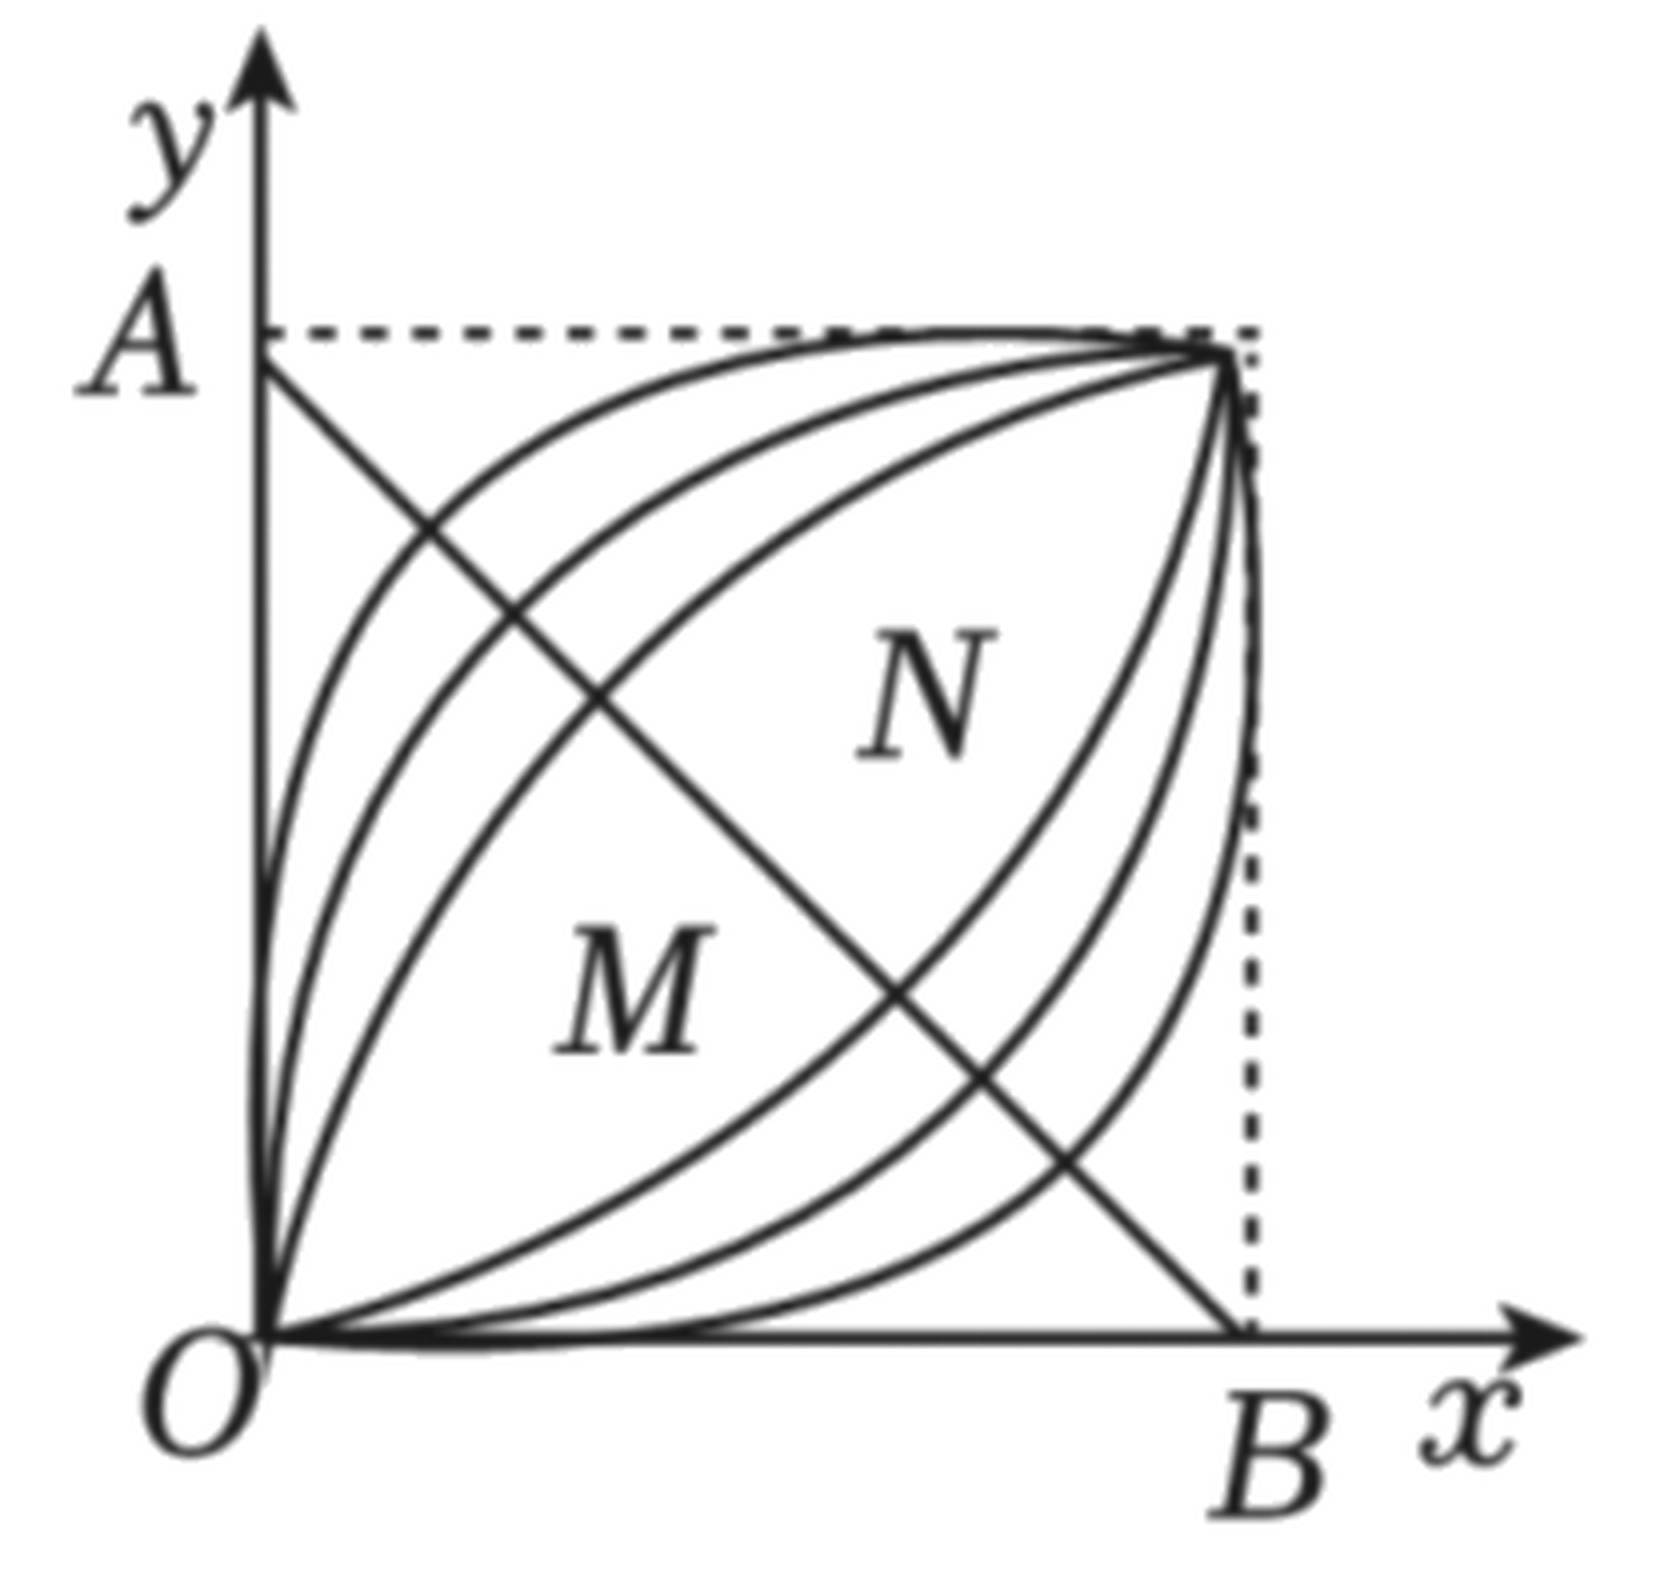
\includegraphics[width=0.40\textwidth]{figures/gao148_q12.png}
\end{center}

\ifanswer
\solbegin
\step{$BM=MN=NA$，点 $A(1,0)$，$B(0,1)$，所以 $M\left(\dfrac{1}{3},\dfrac{2}{3}\right)$，$N\left(\dfrac{2}{3},\dfrac{1}{3}\right)$，}
\step{分别代入 $y=x^\alpha$，$y=x^\beta$，$\alpha=\log_{\frac{2}{3}}\dfrac{1}{3},\beta=\log_{\frac{1}{3}}\dfrac{2}{3}$，$\alpha\beta=\log_{\frac{1}{3}}\dfrac{2}{3}\cdot\log_{\frac{2}{3}}\dfrac{1}{3}=1$.}
\solend
\fi

\end{enumerate}

\bigsec{二、选择题}

\begin{enumerate}
\setcounter{enumi}{12}

% === Q13 ===：答案"C"直接印在题干括号内、全卷无该题【答案】/【解析】段，按 高一84 Q13 成例括号留空、另提 \ans{$C$}；弯引号含空格
\item 若 $x$、$y\in\R$，则 “ $x=0$ ” 是 “ $xy=0$ ” 的\mbox{（\quad）}

\keepwithprev
A. 充要条件\qquad\qquad B. 必要不充分条件

C. 充分不必要条件\qquad\qquad D. 既不充分也不必要条件

\ifanswer
\ans{$C$}
\fi

% === Q14 ===：六个结论（圈数字在文本模式）、四选项一行；解析 8 行（对② 的两行公式各占一印刷行）
\item 若 $a<b<0$，下面有六个结论：① $a^2>b^2$；② $a^3<b^3$；③ $\dfrac{1}{a}<\dfrac{1}{b}$；④ $\dfrac{a}{b}>1$；⑤ $\dfrac{1}{a-b}>\dfrac{1}{a}$；⑥ $\lvert a\rvert>-b$. 其中正确的个数是\mbox{（\quad）}

\keepwithprev
A. 1\qquad\qquad B. 2\qquad\qquad C. 3\qquad\qquad D. 4

\ifanswer
\solbegin
\step{对①：$a^2-b^2=(a+b)(a-b),a+b<0,a-b<0$，故 $a^2-b^2>0$，正确；}
\step{对②：$a^3-b^3=(a-b)(a^2+ab+b^2)=(a-b)\left[\left(a+\dfrac{1}{2}b\right)^2+\dfrac{3}{4}b^2\right],a-b<0$，}
\step{$\left(a+\dfrac{1}{2}b\right)^2+\dfrac{3}{4}b^2>0$，故 $a^3-b^3<0$，正确；}
\step{对③：取 $a=-2,b=-1$，则 $\dfrac{1}{a}=-\dfrac{1}{2},\dfrac{1}{b}=-1,\dfrac{1}{a}>\dfrac{1}{b}$，错误；}
\step{对④：$\dfrac{a}{b}-1=\dfrac{a-b}{b},a-b<0,b<0$，故 $\dfrac{a}{b}-1>0$，正确；}
\step{对⑤：取 $a=-2,b=-1$，则 $\dfrac{1}{a-b}=-1,\dfrac{1}{a}=-\dfrac{1}{2},\dfrac{1}{a-b}<\dfrac{1}{a}$，错误；}
\step{对⑥：要证 $\lvert a\rvert>-b$，即 $-a>-b$，即 $a<b$，正确；}
\step{故选 $D$.}
\solend
\fi

% === Q15 ===：题目配图（四条指数函数曲线，三版都出），\needvspace 守卫放 \item 之前；"图象"照录；解析 5 行
\needvspace{8cm}
\item 如图，曲线①②③④分别是指数函数 $y=a^x$，$y=b^x$，$y=c^x$，$y=d^x$ 的图象，则实数 $a$、$b$、$c$、$d$ 的大小关系为\mbox{（\quad）}

\keepwithprev
A. $a<b<c<d$\qquad B. $b<a<d<c$\qquad C. $d<c<b<a$\qquad D. $c<d<a<b$

\begin{center}
% 四条指数函数曲线图取 04 页右侧，去粉色水印、去色、4× LANCZOS 放大；三版都出
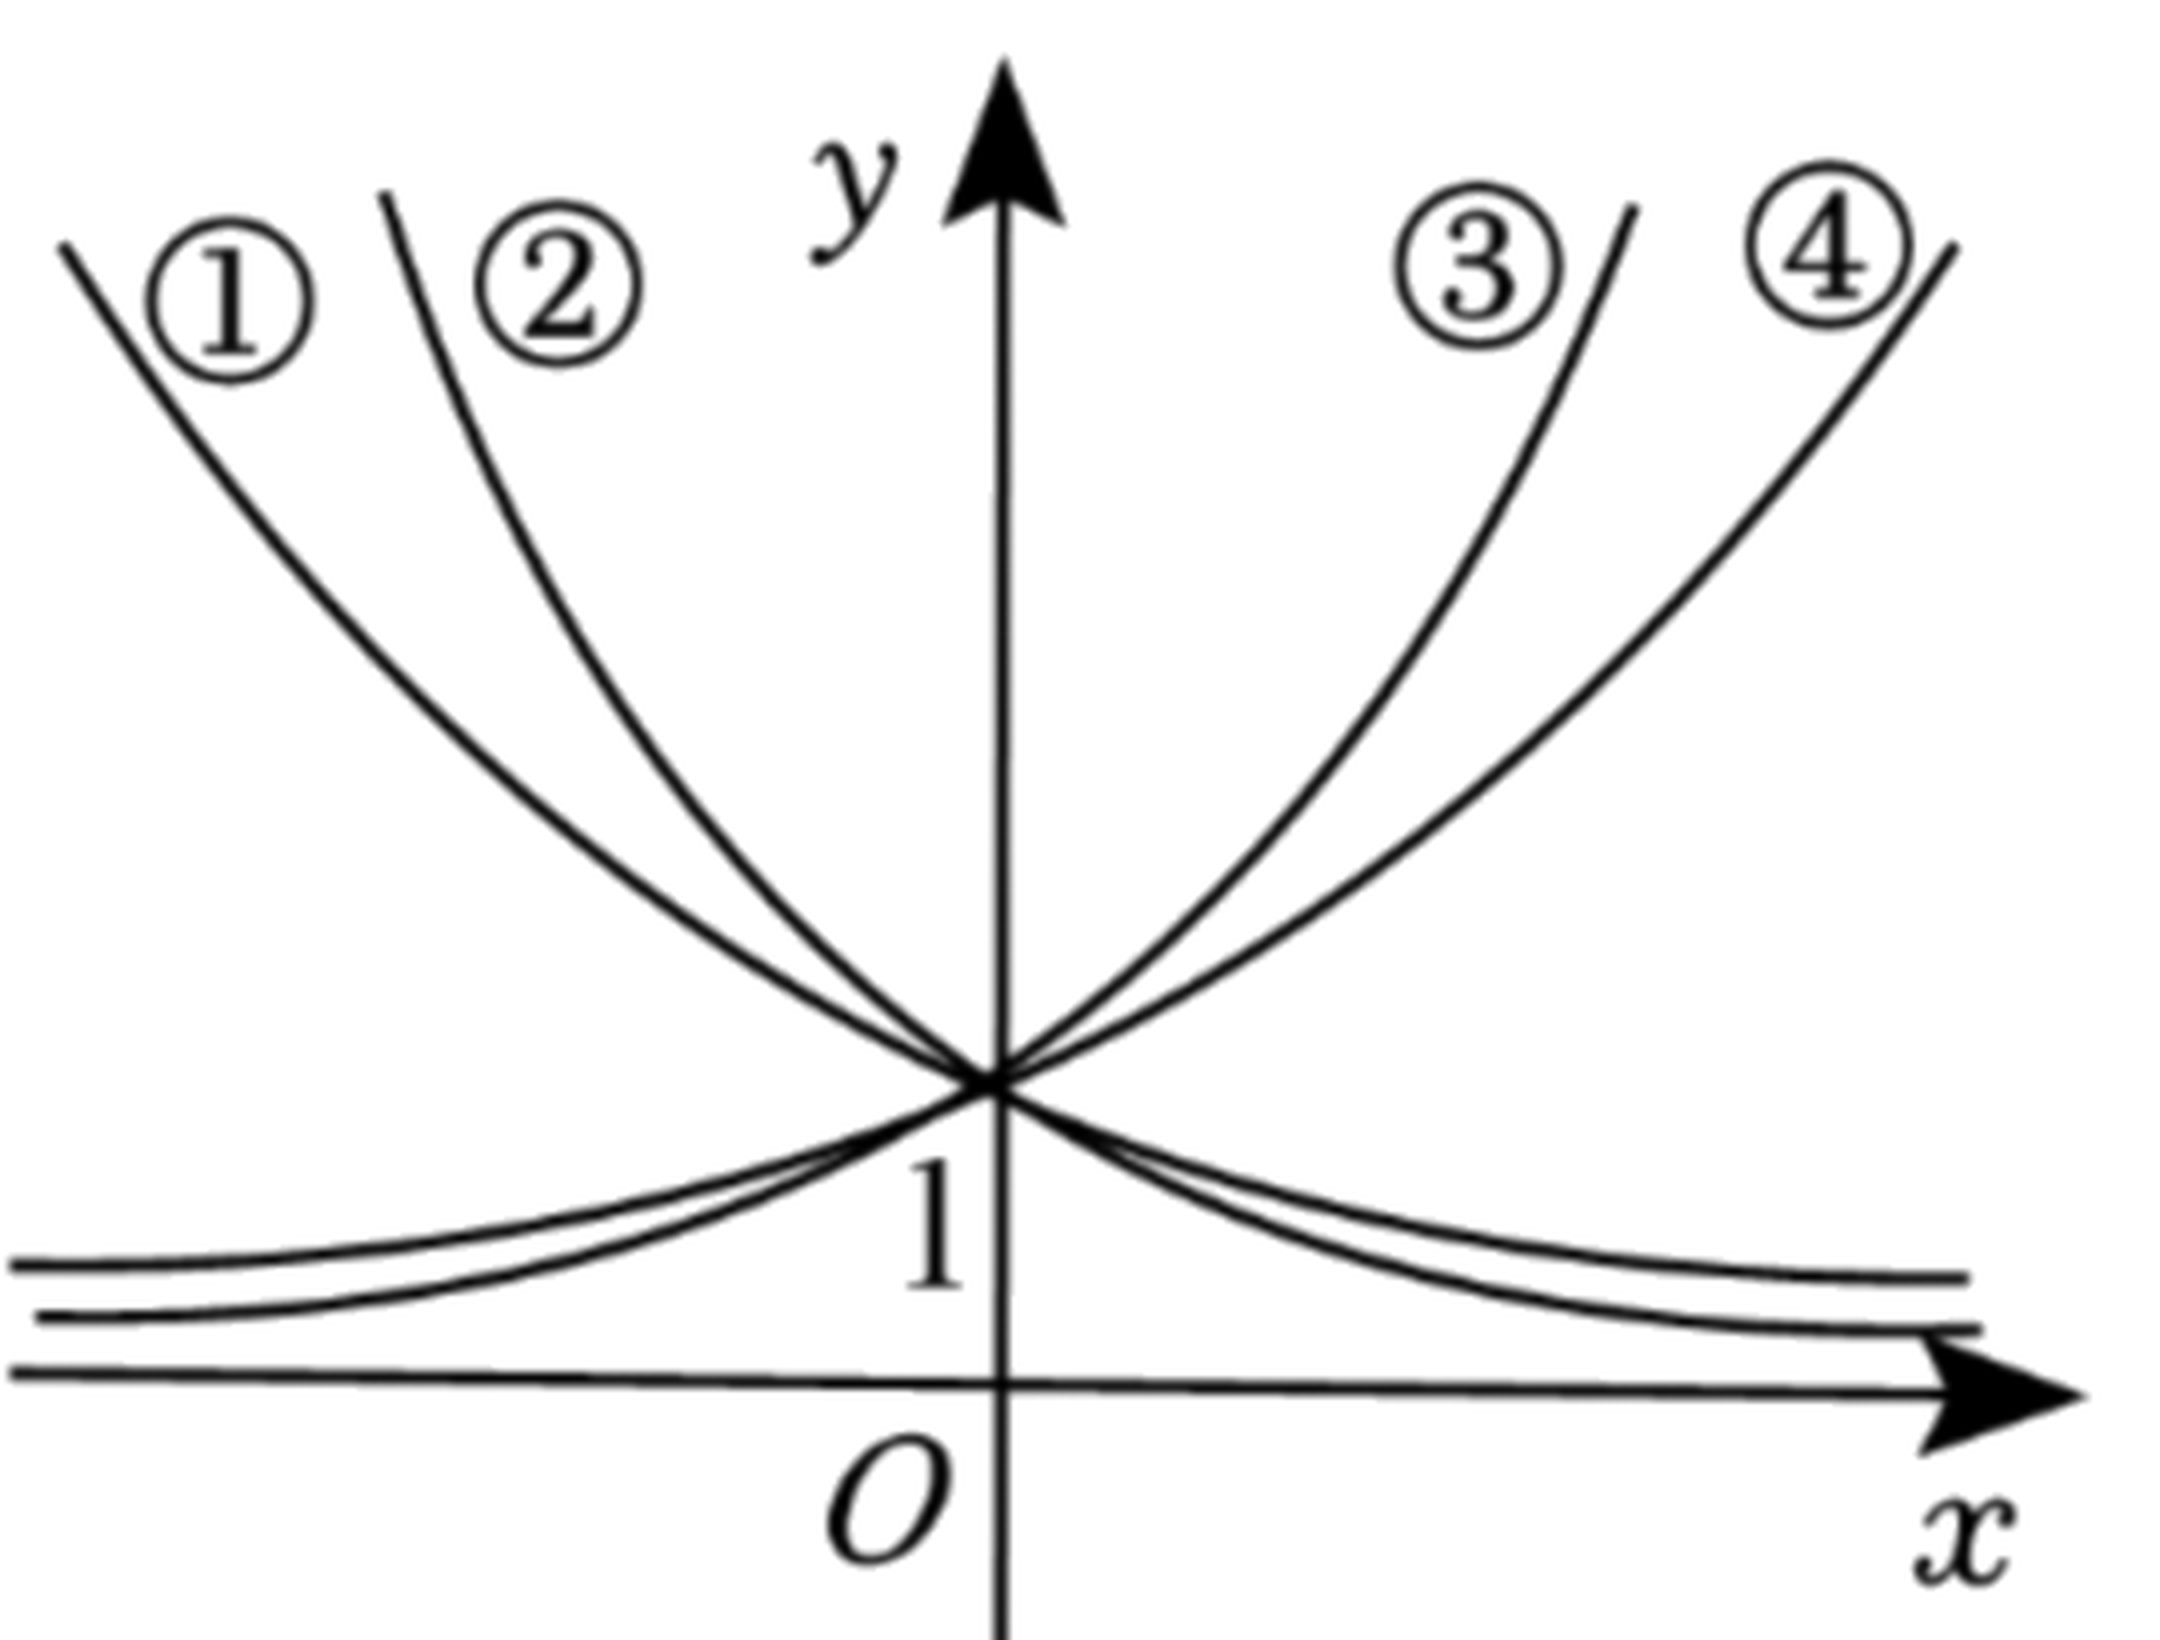
\includegraphics[width=0.40\textwidth]{figures/gao148_q15.png}
\end{center}

\ifanswer
\solbegin
\step{由函数图象得函数① $y=a^x$；② $y=b^x$ 为减函数，且 $x=1$ 时，$b^1<a^1$，}
\step{所以 $0<b<a<1$，}
\step{由函数图象得函数③ $y=c^x$；④ $y=d^x$ 为增函数，且 $x=1$ 时，$c^1>d^1$，}
\step{所以 $c>d>1$，}
\step{所以 $b<a<d<c$. 故选 $B$.}
\solend
\fi

% === Q16 ===：题目配图（关于 y 轴对称的幂函数曲线，三版都出），\needvspace 守卫放 \item 之前；$p$、$q\in\Z$；"图象"照录；解析 2 行
\needvspace{8cm}
\item 已知幂函数 $y=x^{\frac{p}{q}}$（$p$、$q\in\Z$ 且 $p$、$q$ 互质）的图象关于 $y$ 轴对称，如图所示，则\mbox{（\quad）}

\keepwithprev
A. $p$、$q$ 均为奇数，且 $\dfrac{p}{q}>0$\qquad\qquad B. $q$ 为偶数，$p$ 为奇数，且 $\dfrac{p}{q}<0$

C. $q$ 为奇数，$p$ 为偶数，且 $\dfrac{p}{q}>0$\qquad\qquad D. $q$ 为奇数，$p$ 为偶数，且 $\dfrac{p}{q}<0$

\begin{center}
% 关于 y 轴对称的幂函数曲线图取 04 页右下，去粉色水印、去色、4× LANCZOS 放大；三版都出
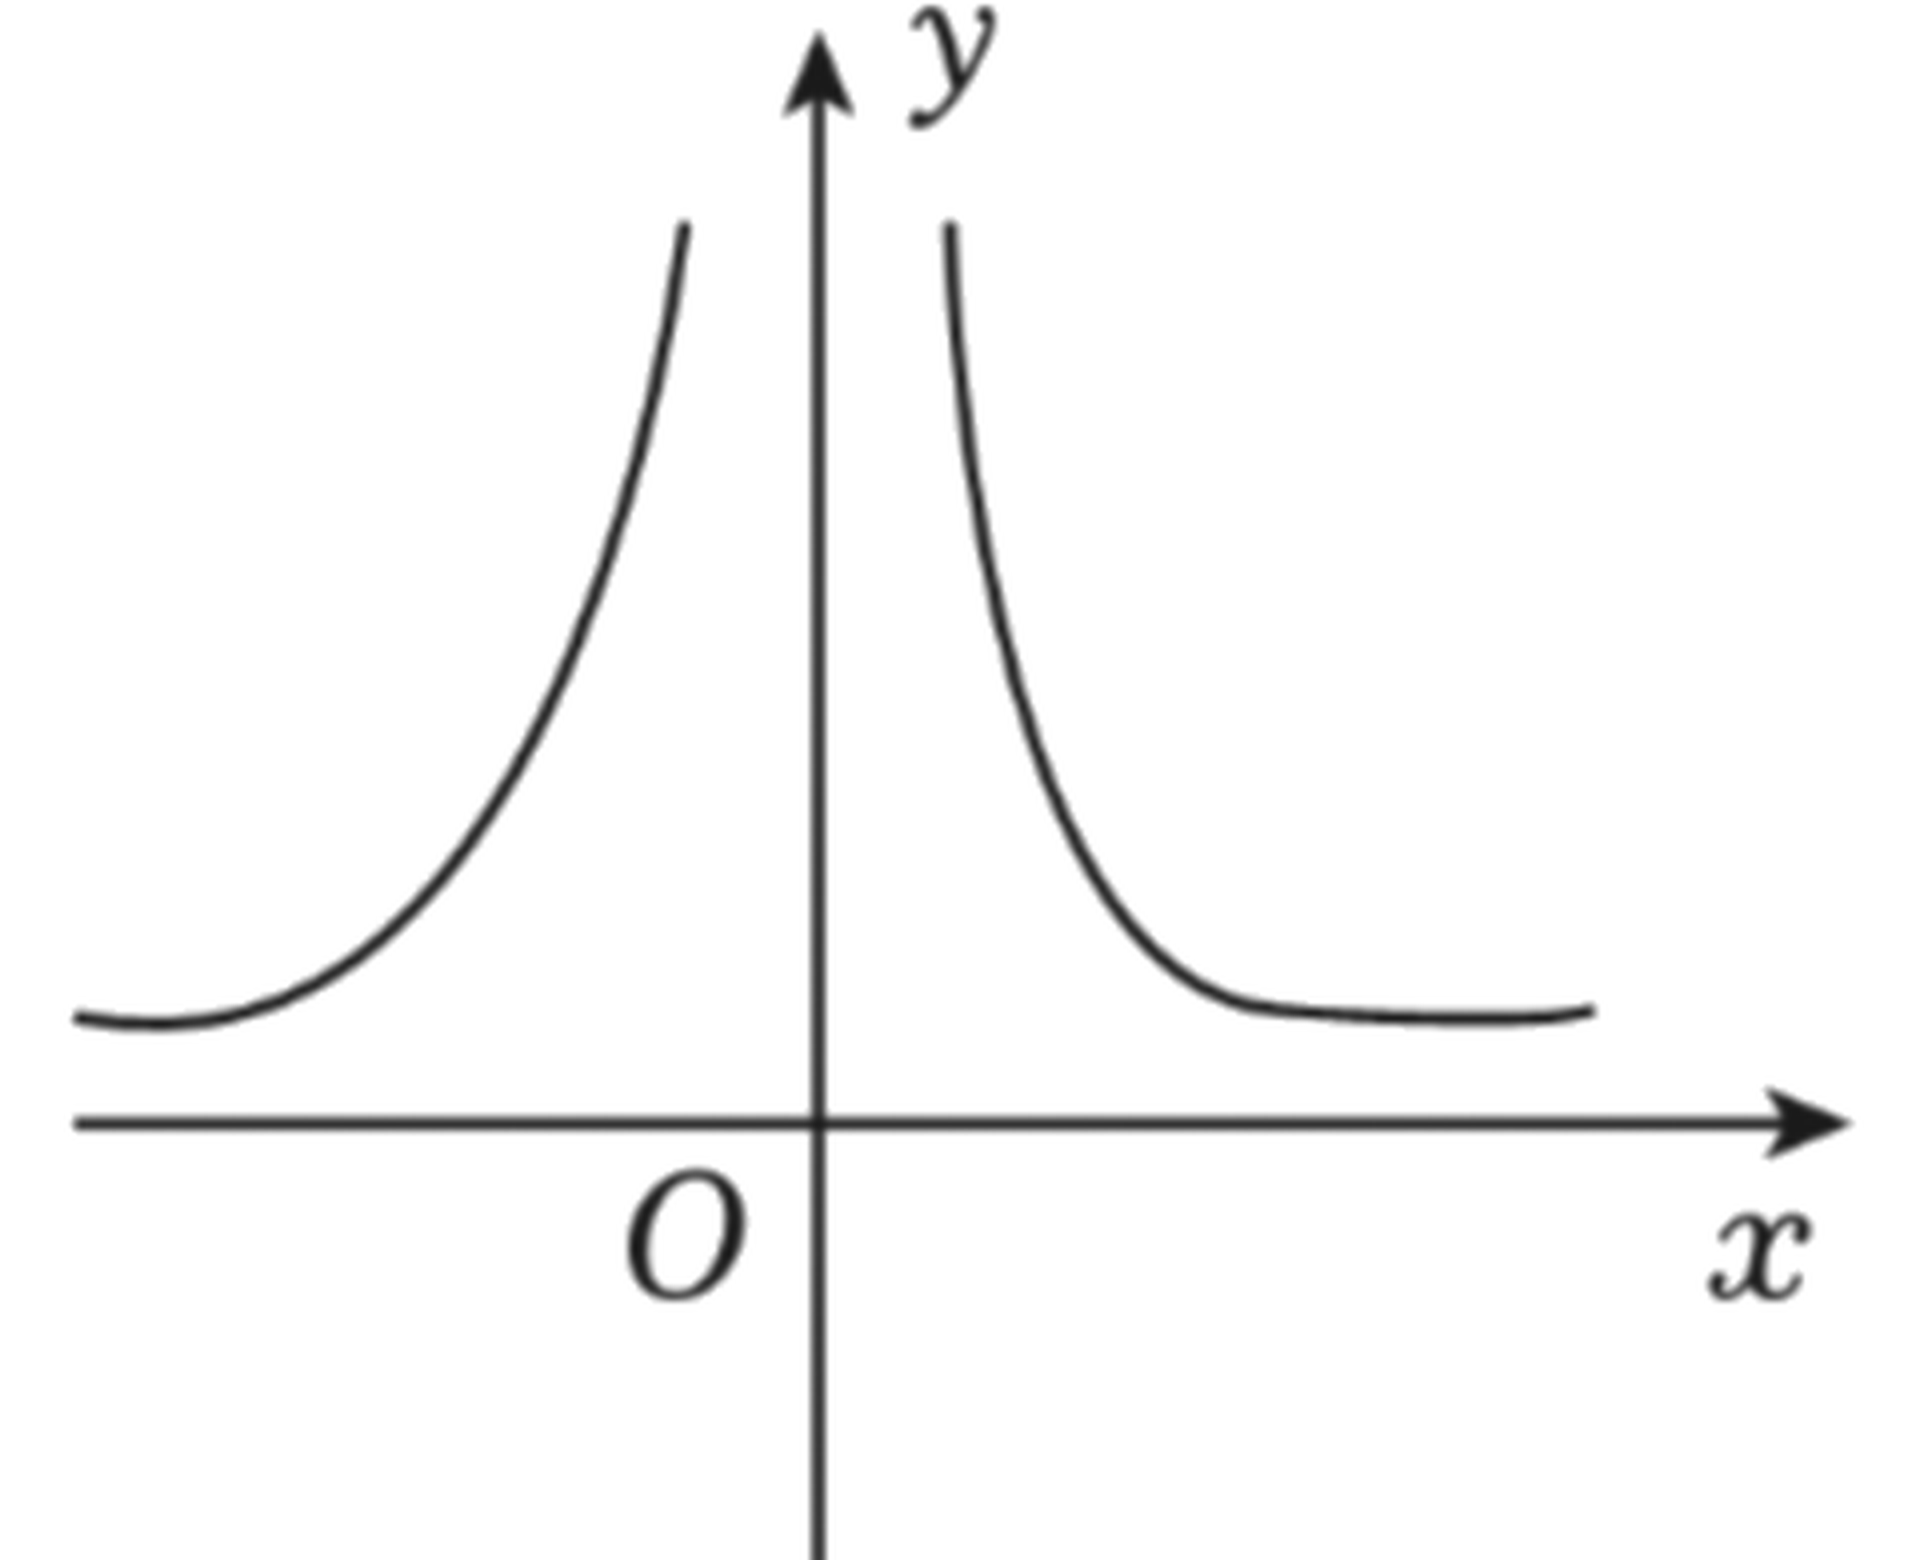
\includegraphics[width=0.36\textwidth]{figures/gao148_q16.png}
\end{center}

\ifanswer
\solbegin
\step{因为函数为偶函数，所以 $p$ 为偶数，且由图象形状判定 $\dfrac{p}{q}<0$.}
\step{又 $p$、$q$ 互质，所以 $q$ 为奇数. 故选 $D$.}
\solend
\fi

\end{enumerate}

\bigsec{三、解答题}

\begin{enumerate}
\setcounter{enumi}{16}

% === Q17 ===：\overline{B}／\varnothing／\R／\mid 逐处照录；解析 8 行
\item 已知集合 $A=\left\{x\mid \dfrac{5}{2x+1}>1\right\}$，$B=\{x\mid x^2+(a+3)x+3a<0,a\in\R\}$.

(1) 求 $A$.

(2) 若全集 $U=\R$，且 $A\cap\overline{B}=\varnothing$，求实数 $a$ 的取值范围.

\ifanswer
\solbegin
\step{(1) $\dfrac{5}{2x+1}>1$，即 $\dfrac{5}{2x+1}-1>0$，即 $\dfrac{4-2x}{2x+1}>0$，即 $(2x+1)(x-2)<0$，}
\step{解得 $-\dfrac{1}{2}<x<2$，所以 $A=\left(-\dfrac{1}{2},2\right)$；}
\step{(2) $x^2+(a+3)x+3a<0$，即 $(x+3)(x+a)<0$，}
\step{全集 $U=\R$，且 $A\cap\overline{B}=\varnothing$，}
\step{当 $a<3$ 时，解得 $-3<x<-a$，则 $\overline{B}=(-\infty,-3)\cup(-a,+\infty)$，}
\step{此时 $-a\geqslant2$，解得 $a\leqslant-2$，}
\step{当 $a\geqslant3$ 时，不满足 $A\cap\overline{B}=\varnothing$，}
\step{故实数 $a$ 的取值范围是 $(-\infty,-2]$.}
\solend
\fi

% === Q18 ===：cases 块整体算一个印刷行；解析 6 行
\item 已知幂函数经过点 $(2,4)$.

(1) 当 $x=\dfrac{1}{2}$ 时，求函数的值；

(2) 是否存在实数 $m$、$n$，使得该函数在区间 $[m,n]$ 上最小值为 $6m-8$，最大值为 $6n-8$？若存在，求出 $m$、$n$ 的值，若不存在，请说明理由.

\ifanswer
\solbegin
\step{(1) 设幂函数的解析式是 $y=x^\alpha$，则 $2^\alpha=4$，解得 $\alpha=2$，}
\step{故 $f(x)=x^2$，$f\left(\dfrac{1}{2}\right)=\dfrac{1}{4}$；}
\step{(2) 因为 $f(x)\geqslant0$，所以 $6m-8\geqslant0$，$m\geqslant\dfrac{4}{3}$，}
\step{由函数 $f(x)$ 在 $(0,+\infty)$ 严格增，得函数 $f(x)$ 在 $(m,n)$ 严格增，}
\step{所以 $\begin{cases}f(m)=6m-8\\f(n)=6n-8\end{cases}$ 且 $m<n$，解得 $m=2$，$n=4$，}
\step{故存在 $m=2$，$n=4$ 满足题意.}
\solend
\fi

% === Q19 ===：7 处评分档照 高一54／64 成例排 \dots\dots N 分；判别式高 \Delta；解析 9 行
\item 已知方程 $x^2+6mx+9m-2=0$，且 $x_1,x_2$ 是方程的两个不同的实数根.

(1) 若 $m=1$，求 $\dfrac{1}{x_1}+\dfrac{1}{x_2}$ 的值；

(2) 若 $m\in\R$，且 $x_1^2+x_2^2<4$，求 $m$ 取值范围.

\ifanswer
\solbegin
\step{(1) 当 $m=1$ 时，方程为 $x^2+6x+7=0$，\dots\dots1 分}
\step{则 $x_1+x_2=-6,x_1\cdot x_2=7$，\dots\dots2 分}
\step{$\dfrac{1}{x_1}+\dfrac{1}{x_2}=\dfrac{x_1+x_2}{x_1\cdot x_2}=-\dfrac{6}{7}$\dots\dots3 分}
\step{(2) $x_1+x_2=-6m,x_1\cdot x_2=9m-2$\dots\dots2 分}
\step{因为 $x_1^2+x_2^2=(x_1+x_2)^2-2x_1\cdot x_2$，所以 $(x_1+x_2)^2-2x_1\cdot x_2<4$，}
\step{所以 $36m^2-2(9m-2)<4$，解得 $0<m<\dfrac{1}{2}$\dots\dots2 分}
\step{又因为方程有两个不同的根，所以 $\Delta=36m^2-4(9m-2)>0$，}% 判别式原卷印等腰偏高粗三角 $\Delta$，照录（放大 07 页 q19_delta3.png／diag_band_q19.png 确认）
\step{解得 $m<\dfrac{1}{3}$ 或 $m>\dfrac{2}{3}$\dots\dots2 分}
\step{所以 $0<m<\dfrac{1}{3}$\dots\dots2 分}
\solend
\fi

% === Q20 ===：题目配图（矩形蔬菜温室，三版都出），\needvspace 守卫放 \item 之前；单位 \mathrm{m}／\mathrm{m}^2；解析 10 行
\needvspace{8cm}
\item 某村计划建造一个室内面积为 $600\mathrm{m}^2$ 的矩形蔬菜温室，在室内，沿左、右两侧与后侧内墙各保留 $2\mathrm{m}$ 宽的通道，沿前侧内墙保留 $4\mathrm{m}$ 宽的空地.

\begin{center}
% 矩形蔬菜温室示意图取 07 页右侧，去粉色水印、去色、4× LANCZOS 放大；三版都出
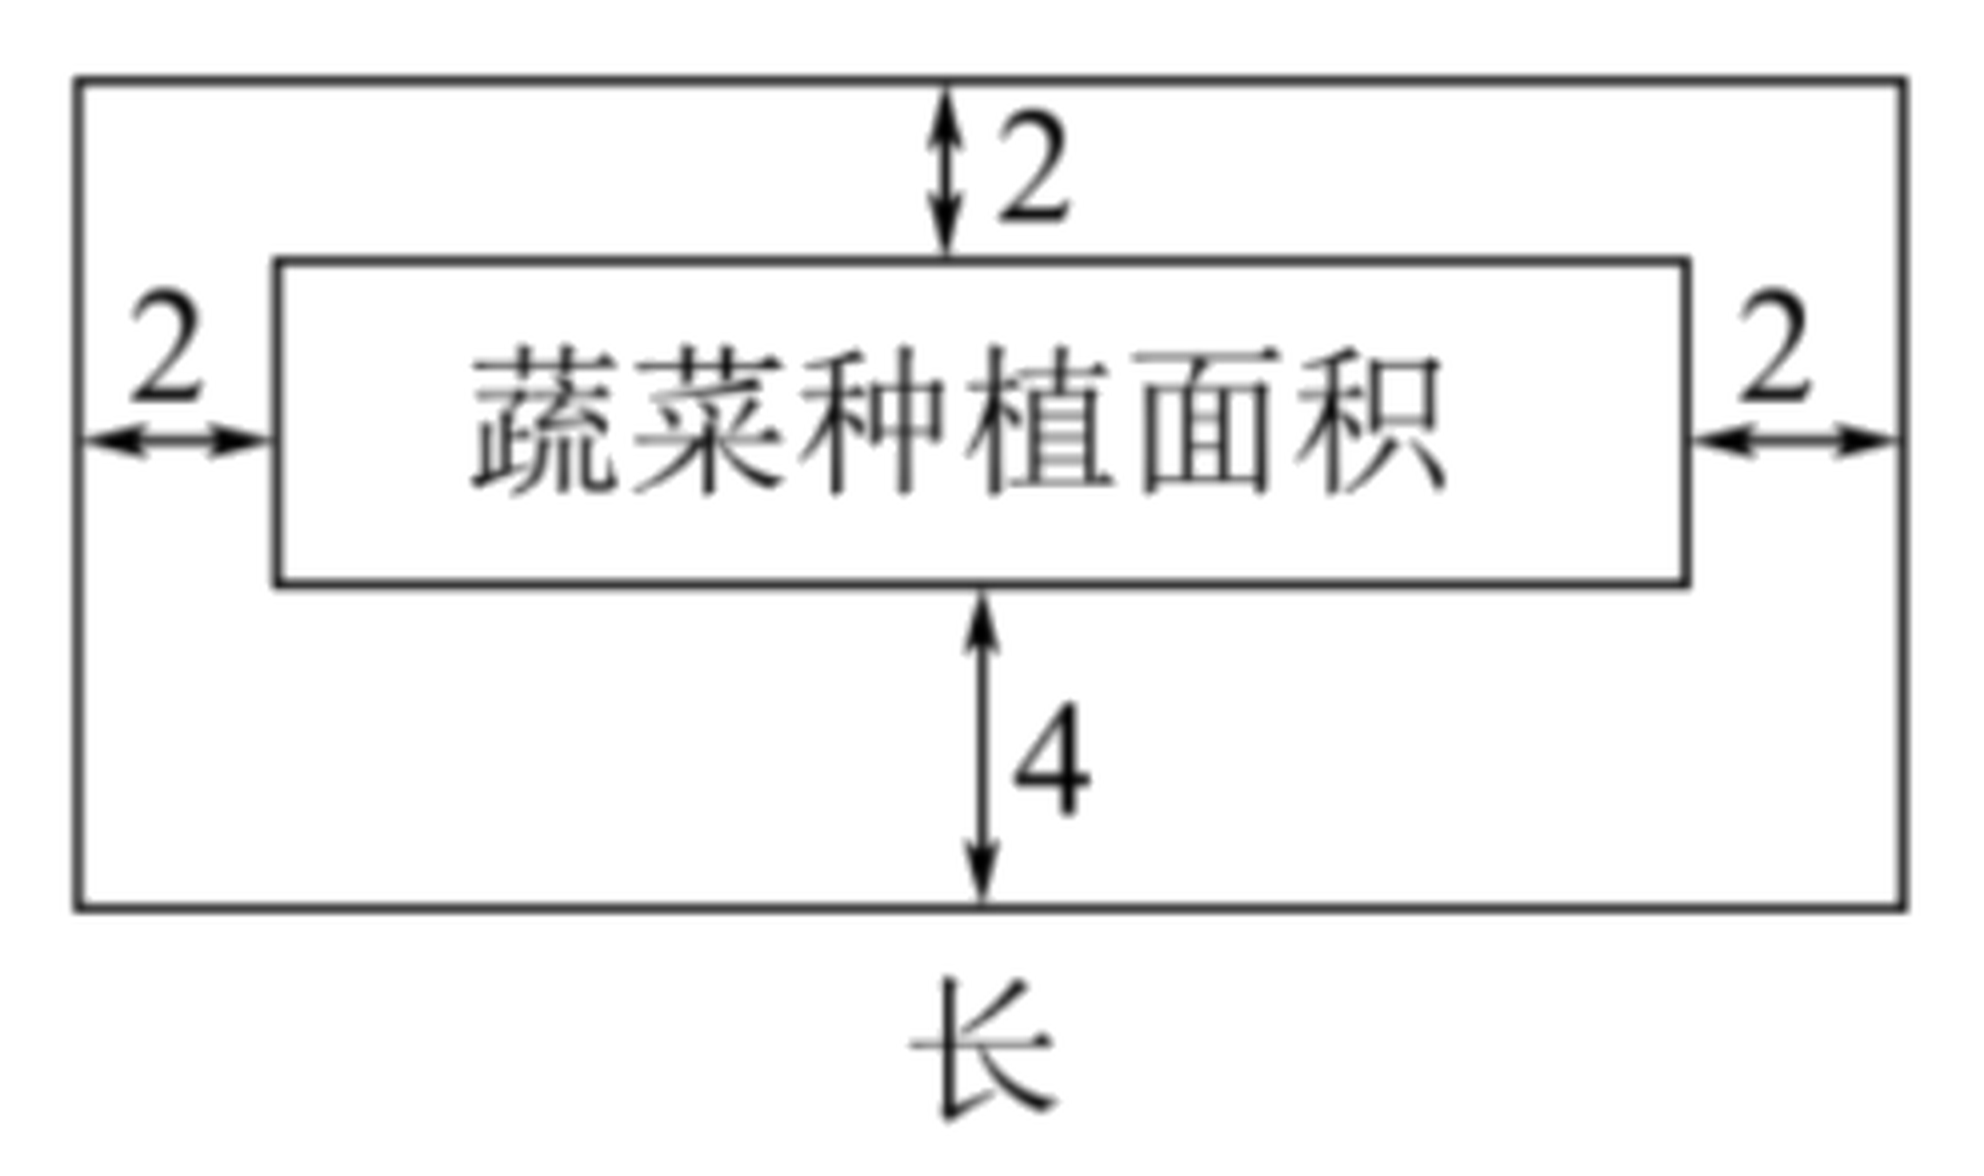
\includegraphics[width=0.45\textwidth]{figures/gao148_q20.png}
\end{center}

(1) 写出蔬菜的种植面积关于矩形温室的长之间的关系式.

(2) 当矩形温室的边长各为多少时，蔬菜的种植面积最大？最大种植面积是多少？

\ifanswer
\solbegin
\step{(1) 设蔬菜的种植面积为 $y\mathrm{m}^2$，矩形温室的长为 $x\mathrm{m}$，}
\step{则矩形温室的宽为 $\dfrac{600}{x}\mathrm{m}$，}
\step{种植蔬菜矩形的长为 $(x-4)\mathrm{m}$，宽为 $\left(\dfrac{600}{x}-6\right)\mathrm{m}$，}
\step{所以 $y=(x-4)\left(\dfrac{600}{x}-6\right)(4<x<100)$；}
\step{(2) 因为 $y=(x-4)\left(\dfrac{600}{x}-6\right)=624-\left(6x+\dfrac{2400}{x}\right)$，}
\step{因为 $6x+\dfrac{2400}{x}\geqslant2\sqrt{6x\cdot\dfrac{2400}{x}}=240$，}
\step{当且仅当 $6x=\dfrac{2400}{x}$，即 $x=20$ 时取等号，}
\step{所以 $y=624-\left(6x+\dfrac{2400}{x}\right)\leqslant624-240=384$.}
\step{即当矩形温室的一边长为 $20\mathrm{m}$，另一边长为 $30\mathrm{m}$ 时，}
\step{蔬菜的种植面积最大，最大为 $384\mathrm{m}^2$.}
\solend
\fi

% === Q21 ===：3 问、cases 块整体算一个印刷行；判别式高 \Delta；解析 19 行（末行续 09 页）
\item 二次函数 $f(x)=ax^2+bx+c$ 满足对任意的 $x\in\R$，$x-1\leqslant f(x)\leqslant x^2-x$ 恒成立.

(1) 求证：$f(1)$ 为定值；

(2) 若 $f(0)=-\dfrac{1}{4}$，求二次函数 $f(x)$ 的表达式；

(3) 求 $a+2b+5c$ 的取值范围.

\ifanswer
\solbegin
\step{(1) 对任意的 $x\in\R$，$x-1\leqslant f(x)\leqslant x^2-x$ 恒成立，则 $0\leqslant f(1)\leqslant0$，}
\step{所以 $f(1)=0$，为定值.}
\step{(2) 由(1)得 $a+b+c=f(1)=0$，由 $f(0)=-\dfrac{1}{4}$，得 $c=-\dfrac{1}{4}$，}
\step{则 $b=\dfrac{1}{4}-a$，$f(x)=ax^2+\left(\dfrac{1}{4}-a\right)x-\dfrac{1}{4}$，}
\step{不等式 $x-1\leqslant f(x)$ 可化为 $ax^2+\left(\dfrac{1}{4}-a\right)x-\dfrac{1}{4}\geqslant x-1$，}
\step{即 $ax^2-\left(a+\dfrac{3}{4}\right)x+\dfrac{3}{4}\geqslant0$，}
\step{一元二次不等式 $ax^2-\left(\dfrac{3}{4}+a\right)x+\dfrac{3}{4}\geqslant0$ 恒成立，则 $\begin{cases}a>0\\\Delta=\left(a+\dfrac{3}{4}\right)^2-3a\leqslant0\end{cases}$，}% 判别式原卷印等腰偏高粗三角 $\Delta$，照录（放大 08 页 q21_delta3.png／diag_band_q21.png 确认）
\step{解得 $a=\dfrac{3}{4}$，}
\step{此时 $f(x)=\dfrac{3}{4}x^2-\dfrac{1}{2}x-\dfrac{1}{4}$，$x^2-x-f(x)=\dfrac{1}{4}(x-1)^2\geqslant0$ 恒成立，}
\step{所以 $f(x)=\dfrac{3}{4}x^2-\dfrac{1}{2}x-\dfrac{1}{4}$.}
\step{(3) 由(1)得 $b=-a-c$，$f(x)=ax^2-(a+c)x+c=(ax-c)(x-1)$，}
\step{不等式 $x-1\leqslant f(x)$ 可化为 $(x-1)(ax-c-1)\geqslant0$，}
\step{一元二次不等式 $(x-1)(ax-c-1)\geqslant0$ 恒成立，则 $a>0$，}
\step{且方程 $(x-1)(ax-c-1)=0$ 有相等的实数根，因此 $c=a-1$，$a>0$，}
\step{不等式 $f(x)\leqslant x^2-x\Leftrightarrow(ax-c)(x-1)\leqslant x^2-x\Leftrightarrow(x-1)[(1-a)x+c]\geqslant0$，}
\step{同理 $1-a>0$，且方程 $(x-1)[(1-a)x+c]=0$ 有相等的实数根，}
\step{因此 $c=a-1$，$a<1$，从而 $c=a-1$，$b=1-2a$，$0<a<1$，}
\step{$a+2b+5c=a+2(1-2a)+5(a-1)=2a-3\in(-3,-1)$，}
\step{所以 $a+2b+5c$ 的取值范围是 $(-3,-1)$.}
\solend
\fi

\end{enumerate}

\end{document}
"
% 紧凑版：xelatex "\def\iscompact{1}% 高一148_新川中学_期中.tex
%   —— 高一上数学"2026-2027 年新川中学高一上期中"（试卷版/答案版/紧凑版）
% 试卷版：xelatex 高一148_新川中学_期中.tex
% 答案版：xelatex "\def\isanswer{1}% 高一148_新川中学_期中.tex
%   —— 高一上数学"2026-2027 年新川中学高一上期中"（试卷版/答案版/紧凑版）
% 试卷版：xelatex 高一148_新川中学_期中.tex
% 答案版：xelatex "\def\isanswer{1}% 高一148_新川中学_期中.tex
%   —— 高一上数学"2026-2027 年新川中学高一上期中"（试卷版/答案版/紧凑版）
% 试卷版：xelatex 高一148_新川中学_期中.tex
% 答案版：xelatex "\def\isanswer{1}\input{高一148_新川中学_期中.tex}"
% 紧凑版：xelatex "\def\iscompact{1}\input{高一148_新川中学_期中.tex}"
%
% ① 原始材料：微信公众号"魔都数学加油站"文章，连载"27学年高一148"，原文标题
% "27学年高一148——2026-2027年上海市新川中学高一上期中"（2026-11-21 推送）；
% 原文链接：https://mp.weixin.qq.com/s/Alhmwb3sSLQMp_wjzoAVyA 。
% 正文为 9 张 PNG 页（01/03/04/07/08/09 为 2560×3620，02/05/06 为 4762×6735，
% 同一篇各页分辨率混排，逐页按各自分辨率裁图核对，别按预览比例换算裁框）。
% 体例：混合体例讲评版——19 题中 Q4、Q5 只印【答案】、无【解析】；Q13 的答案"C"
% 直接印在题干括号内、无【答案】/【解析】段；其余 16 题印【解析】（逐题核实，见 ② ②）。
% 题目、答案、解析均据原图转录；卷面粉红色水印"魔都数学加油站"及公众号页脚未录入。
% 全卷插图清单（逐页通读 9 页确认）：4 幅题目配图，均三版都出、均非【解析】内配图：
%   · Q12 幂函数曲线族图（03 页右侧：x/y 轴、O、A(1,0)、B(0,1)、M、N 与两族
%     y=x^α／y=x^β 曲线、线段 AB、虚线），题干"（如图）"处，裁 figures/gao148_q12.png；
%   · Q15 四条指数函数曲线图（04 页右侧：①②③④ 四曲线同过 (0,1)、x/y 轴、O、
%     y 轴刻度 1），题干"如图"处，裁 figures/gao148_q15.png；
%   · Q16 关于 y 轴对称的幂函数曲线图（04 页右下：x/y 轴、O、两支上翘曲线），
%     题干"如图所示"处，裁 figures/gao148_q16.png；
%   · Q20 矩形蔬菜温室示意图（07 页右侧：大矩形＋内框"蔬菜种植面积"＋2/2/4
%     通道标注＋"长"），题干处，裁 figures/gao148_q20.png；
%   其余各页逐页确认无其它题目配图、无【解析】内配图、无表格，亦无"题干写如图而
%   源码漏图"一处；Q19 解析行末的虚线"----N 分"为评分档（非图），Q18／Q21 的
%   cases 块为数学块（非图）。4 图均取自原卷截图，去粉色水印、去色、4× LANCZOS 放大。
%
% 卷首标题：原卷印作"2026-2027 年新川中学高一上期中"，年份区间按全稿惯例排 en dash；
% 原卷卷面未印副标题，本稿按同期中卷（高一140／141／143／144／145／146／147）知识模块
% 口径补出"集合与常用逻辑用语、不等式、函数"。
%
% 题号体例（逐页核实定稿）：本卷共 19 题——一、填空题 3—12（10 题）、
% 二、选择题 13—16（4 题）、三、解答题 17—21（5 题）。
% 三节分别 \setcounter{enumi}{2}／{12}／{16}。原卷从第 3 题起、无第 1、2 题，
% 本稿保留原题号；全卷无附加题节、无 Q22（Q21 解析末行"所以 a+2b+5c 的取值范围是
% (-3,-1)."为全卷收尾，09 页下半仅水印、无正文）。
%
% ② 与原卷的排版差异：
%   ① 原文从第 3 题起，本稿保留原题号；共 19 题三节；
%   ② 混合体例逐题核实：Q4（反证法"假设的内容"）、Q5 只印【答案】、无【解析】，
%      按 高一140 第 5 题／高一145 Q3 成例提 \ans{}、不补造解析；Q13 答案"C"直接
%      印在题干括号内（" ( C ) "）、全卷无该题【答案】/【解析】段，按 高一84 Q13／
%      高一37 Q13／高一53 Q13 成例括号 \mbox{（\quad）} 留空、另提 \ans{$C$}；
%      其余 16 题印【解析】、用 \solbegin…\solend，选择题答案在解析末句"故选 X"
%      （Q14 选 D、Q15 选 B、Q16 选 D，逐个放大原图核实）、题干括号留空、不另提
%      \ans{}；答案版【答案】/【解析】标记数 = 19（3 个 \ans ＋ 16 个 \solbegin）
%      = 全卷题数；
%   ③ 原卷卷面未印副标题，本稿按知识模块口径补出；
%   ④ 原卷填空横线按全稿惯例排 \blankline[4.4em]；选择题括号排 \mbox{（\quad）}、
%      选项段前按惯例加 \keepwithprev；Q13／Q16 四选项为两行两列、Q14／Q15 选项
%      为一行，照原卷分行；解答题不留作答区、不加 \anspace（原卷为讲评版，
%      与 129／131／132／133／136／140／141／143／144／145／146 同）；
%   ⑤ 数集：Q11"在 R 上定义运算"、Q13"x、y∈R"、Q16"p、q∈Z"、Q17"a∈R"
%      "U=R"、Q19"m∈R"、Q21"x∈R" 原卷印斜体 R/Z，按全稿惯例统一改 \R／\Z
%      （本卷未出现 N，\N^* 无对应处）；绝对值排 \lvert…\rvert（Q9／Q14），
%      集合描述竖线排 \mid（Q17）；不等号按全稿惯例排 \leqslant／\geqslant；
%      补集照原卷上划线排 \overline{B}（Q17 题干 1 处＋解析 3 处）；空集
%      \varnothing（Q17 题干 1 处＋解析 2 处）；\subset（Q3 题干 {a}⊂M）与
%      \subseteq（Q3 题干 M⊆{a,b,c,d}）逐处照录不统一（放大 01 页 q3_subset.png）；
%   ⑥ 子题标号 (1)(2)(3) 半角括号照录；圈数字 ①—⑥ 在文本模式（Q14 六个结论、
%      Q15 曲线编号与其解析、Q14 解析"对①…对⑥"），按 common.sty 划入 CJK 字符类
%      渲染；cases 块整体算一个印刷行；\left…\right 不得拆到不同 $…$ 组；
%      单位 m／m² 排 \mathrm{m}／\mathrm{m}^2（Q20，原卷印正体 m）；
%   ⑦ 题干／解析中的中文弯引号按原卷照录：Q4" ab 可以被 5 整除，那么 a、b 中
%      至少有一个能被 5 整除 "（开引号后有空格、闭引号后空格接"时"）、
%      Q13" x=0 "" xy=0 "（引号内空格），注释内一律 ASCII 引号；
%   ⑧ 半角逗号在数学组之间是全稿惯例、非笔误（Q3"{a,b,c,d}"、Q6"$x,y$"
%      "$x=\frac13,y=\frac16$"、Q10、Q11"$a=-2,b=-1"、Q12"$\alpha=\log..,\beta=..$"、
%      Q14"$a+b<0,a-b<0$"、Q17、Q19"$x_1+x_2=-6,x_1\cdot x_2=7$"、Q20、Q21 等），
%      逐处照录别改全角；行末西文句点照录为 ASCII `.`；行中全角逗号／顿号照录；
%   ⑨ "图像／图象"逐处放大核：全卷 9 处均印"图象"（象，无亻）、未见"图像"，
%      逐处照录未统一改动（Q8 题干/解析各 1、Q12 题干 2、Q15 题干 1／解析 2、
%      Q16 题干 1／解析 1；放大 02/03/04/05 页 /tmp/gao148/zoom/my_wide_a.png、
%      my_wide_b.png 与宋体参考"象／像"并排确认）；
%   ⑩ 判别式 Δ/△ 混用是照录项：Q11 解析"△=1−4(−a²+a+1)<0"印扁等边空心
%      三角 \triangle；Q19 解析"Δ=36m²−4(9m−2)>0"、Q21 解析 cases 块
%      "Δ=(a+3/4)²−3a≤0" 两处印等腰偏高粗三角 \Delta，逐处放大判断、照录
%      不统一（参照 高一142／144／145 头注④口径，详见 ④）；
%   ⑪ 一条 \step = 原卷解析的一个印刷行，cases 块整体算一个印刷行；别把原卷折行
%      并起来、别把一行拆多条。Q3 六行、Q7 五行（01 页末首行＋02 页顶四行）、
%      Q9 七行、Q11 五行、Q14 八行（对② 的两行公式各占一印刷行）、Q17 八行、
%      Q18 六行、Q19 九行（7 处评分档附在行末）、Q20 十行、Q21 十九行
%      均按印刷行逐条断，不丢行；
%   ⑫ 配图：4 幅均为题目配图（三版都出），放 \item 内题干之后 \begin{center}；
%      大图块加 \needvspace 守卫把整块推走（守卫放 \item 之前，见 高一145 Q14/Q20
%      成例与切页审计 B 类坑）；三版切页审计均"合计异常：无"；
%   ⑬ 跨页续印按题合并：Q3/4/5 在 01 页；Q6 题干＋解析在 01 页；Q7 题干在 01 页
%      末、解析首行在 01 页末续 02 页顶四行；Q8/9/10 在 02 页（Q9 解析续 02 页下半、
%      Q10 题干与解析前 2 行在 02 页末）；Q10 解析末行续 03 页顶；Q11/12 在 03 页、
%      "二、选择题"标题与 Q13/14 题干在 03 页下半；Q13 无解析；Q14 解析在 04 页顶、
%      Q15 题干＋图＋选项＋解析在 04 页、Q16 题干＋图在 04 页末；Q16 选项＋解析＋
%      "三、解答题"标题＋Q17 题干＋解析在 05 页、Q18 题干首句在 05 页末；Q18 题干
%      续＋解析、Q19 题干＋解析前 5 行在 06 页；Q19 解析续 4 行＋Q20 题干＋图＋
%      解析（10 行全部）在 07 页，末行"蔬菜的种植面积最大，最大为 384m²."收尾；
%      Q21 题干＋解析前 18 行在 08 页；Q21 解析末行"所以 a+2b+5c 的取值范围是
%      (-3,-1)."在 09 页上半（09 页下半仅水印、无正文）。本稿按题连排，不丢行、
%      不并折行；
%   ⑭ 原卷解析内无红色"法一／法二"之类小标题，故本卷无 \stepm；水印
%      "魔都数学加油站"红色不录入；Q19 解析 7 处评分档（1/2/3/2/2/2/2 分）
%      原卷在行末印一串虚线，本稿照 高一54／64 成例排 \dots\dots N 分，
%      分值逐处照录、位置不变。
%
% ③ 行数复核：一条 \step／\stepm = 原卷解析的一个印刷行，cases 块作一个印刷行计。
%   逐题数（主会话逐页核对定稿）：Q3：6；Q4：0（只印【答案】、提 \ans{}）；
%   Q5：0（只印【答案】、提 \ans{}）；Q6：2；Q7：5；Q8：2；Q9：7；Q10：3；
%   Q11：5；Q12：2；Q13：0（答案印在题干括号内、另提 \ans{}）；Q14：8；Q15：5；
%   Q16：2；Q17：8；Q18：6；Q19：9；Q20：10；Q21：19。
%   合计 99 条 \step（本卷无 \stepm：解析内无红色"法一／法二"类小标题），
%   与原卷逐题印刷行相等。全卷 16 题设 \solbegin…\solend ＋ 3 处 \ans{}，
%   答案版【答案】/【解析】标记数 = 19 = 全卷题数。
%
% ④ 判别式／子集符号结论（逐处放大原图照录、不得统一，主会话像素级复核）：
%   判别式全卷 3 处，两形混用逐处照录不统一（参照 高一142／144／145 头注④口径）：
%     · Q11 解析"△=1−4(−a²+a+1)<0" 原卷印扁等边空心三角（宽>高、细线），
%       照录 \triangle（放大 03 页 /tmp/gao148/zoom/q11_delta3.png、
%       delta_montage.png 确认）；
%     · Q19 解析"Δ=36m²−4(9m−2)>0" 原卷印等腰偏高粗三角（高>宽），
%       照录 \Delta（放大 07 页 /tmp/gao148/zoom/q19_delta3.png 确认）；
%     · Q21 解析 cases 块"Δ=(a+3/4)²−3a≤0" 原卷印等腰偏高粗三角（高>宽），
%       照录 \Delta（放大 08 页 /tmp/gao148/zoom/q21_delta3.png 确认）。
%   子集／补集：Q3 题干"{a}⊂M⊆{a,b,c,d}" 前者印单线 ⊂、无下划线，照录 \subset；
%     后者印带下划线 ⊆，照录 \subseteq（放大 01 页 /tmp/gao148/zoom/q3_subset.png
%     确认）；Q17 题干 1 处＋解析 3 处共 4 处 \overline{B} 照原卷上划线
%     （B 上横线、非 C_U B）；空集 \varnothing 3 处（Q17 题干 1 处、解析 2 处）；
%     Q17 集合描述竖线 \mid；数集 \R／\Z 归一见 ② ⑤。
%
% ⑤ 存疑照录（放大原图确认，照录未改、正文对应处另有 % 注）：
%   1. Q3 解析末行"所以 M 一共有 3+3+1+1=8 个" 原卷印 $3+3+1+1=8$，按上文
%      四行应为 $1+3+3+1=8$（疑为原卷加数顺序笔误，和仍为 8），放大 01 页
%      /tmp/gao148/zoom/my_q3_sol.png 确认，照录未改。
%   2. Q13 答案"C"直接印在题干括号内、全卷无该题【答案】/【解析】段，按
%      高一84 Q13 成例括号留空、另提 \ans{$C$}（见 ② ②），未补造解析。
%   3. Q19 解析 7 处评分档（"----N 分"）原卷印一串虚线，本稿照 高一54／64
%      成例排 \dots\dots N 分，分值逐处照录、位置不变。
%   4. 判别式 Q11 扁 \triangle 与 Q19／Q21 高 \Delta 两形混用，逐处照录不统一（见 ④）。
%   5. "图像／图象"全卷 9 处均印"图象"、未见"图像"（见 ② ⑨），逐处放大核实照录，
%      未统一改动。
%   全卷除此 5 类外未发现其它笔误／自相矛盾处。
%
% ⑥ 跨页续印按题合并说明：见 ② ⑬。
%
\documentclass[a4paper,11pt]{article}
\usepackage{common}

\begin{document}

\examtitlest[3]{2026--2027 年新川中学高一上期中}{集合与常用逻辑用语、不等式、函数}

\bigsec{一、填空题}

\begin{enumerate}
\setcounter{enumi}{2}

% === Q3 ===：题干 {a}⊂M⊆{a,b,c,d} 两个子集符号逐处照录；解析 6 行
\item 满足 $\{a\}\subset M\subseteq\{a,b,c,d\}$ 的集合 $M$ 有\blankline[4.4em]个.

\ifanswer
\solbegin
\step{$M$ 是 $\{a,b,c,d\}$ 的子集，但必含有元素 $a$，}
\step{当 $M$ 中只一个元素时，$M=\{a\}$ 只有 1 个；}
\step{当 $M$ 中有二个元素时，$M$ 有 3 个；}
\step{当 $M$ 中有三个元素时，$M$ 有 3 个；}
\step{当 $M$ 中有四个元素时，$M$ 有 1 个；}
\step{所以 $M$ 一共有 $3+3+1+1=8$ 个.}% 原卷印 $3+3+1+1=8$（按上文四行应为 $1+3+3+1$），疑为加数顺序笔误，照录未改（放大 01 页 my_q3_sol.png）
\solend
\fi

% === Q4 ===：原卷只印【答案】、无【解析】，按 高一140 第 5 题成例提 \ans{}；弯引号与空格照录
\item 用反证法证明命题 “ $ab$ 可以被 5 整除，那么 $a$、$b$ 中至少有一个能被 5 整除” 时假设的内容应该是\blankline[4.4em].

\ifanswer
\ans{$a$、$b$ 都不能被 5 整除}
\fi

% === Q5 ===：原卷只印【答案】 $[-2,1)$、无【解析】，提 \ans{}
\item 不等式 $\dfrac{x+2}{x-1}\leqslant0$ 的解集为\blankline[4.4em].

\ifanswer
\ans{$[-2,1)$}
\fi

% === Q6 ===：解析 2 行；半角逗号在数学组之间照录
\item 设 $x,y\in(0,+\infty)$，且 $x+4y=1$，则 $\dfrac{1}{x}+\dfrac{1}{y}$ 的最小值为\blankline[4.4em].

\ifanswer
\solbegin
\step{因为 $\dfrac{1}{x}+\dfrac{1}{y}=(x+4y)\left(\dfrac{1}{x}+\dfrac{1}{y}\right)=5+\dfrac{4y}{x}+\dfrac{x}{y}\geqslant5+2\sqrt{\dfrac{4y}{x}\cdot\dfrac{x}{y}}=9$，}
\step{当且仅当 $\dfrac{4y}{x}=\dfrac{x}{y}$，即 $x=2y$，即 $x=\dfrac{1}{3},y=\dfrac{1}{6}$ 时取等号，故最小值为 9.}
\solend
\fi

% === Q7 ===：题干在 01 页末、解析首行在 01 页末续 02 页顶四行；解析 5 行
\item 若不等式 $x^2+ax+b<0$ 的解集为 $(-3,-1)$，则不等式 $bx^2+ax+1\leqslant0$ 的解集为\blankline[4.4em].

\ifanswer
\solbegin
\step{不等式 $x^2+ax+b<0$ 的解集为 $(-3,-1)$，}
\step{所以方程 $x^2+ax+b=0$ 的两个实数根为 $-3$ 和 $-1$，}
\step{由根与系数的关系得 $a=4$，$b=3$，}
\step{故 $bx^2+ax+1\leqslant0$ 可化为 $3x^2+4x+1\leqslant0$，解得 $-1\leqslant x\leqslant-\dfrac{1}{3}$，}
\step{所求不等式 $bx^2+ax+1\leqslant0$ 的解集为 $\left[-1,-\dfrac{1}{3}\right]$.}
\solend
\fi

% === Q8 ===："图象"照录；解析 2 行
\item 函数 $y=a^{x-2}+2(a>0,a\ne1)$ 的图象必经过定点\blankline[4.4em].

\ifanswer
\solbegin
\step{令 $x-2=0$，得 $x=2$，则 $y=a^0+2=3$，}
\step{所以函数 $y=a^{x-2}+2$ 的图象过定点 $(2,3)$.}
\solend
\fi

% === Q9 ===：解析 7 行；首句末西文句点照录
\item 不等式 $\lvert x+3\rvert+\lvert a-x\rvert>6$ 对一切实数 $x$ 恒成立，则实数 $a$ 的取值范围为\blankline[4.4em].

\ifanswer
\solbegin
\step{$\lvert x+3\rvert$ 表示 $x$ 到 $-3$ 的距离，$\lvert a-x\rvert$ 表示 $x$ 到 $a$ 的距离.}
\step{所以它们的和为 $x$ 到 $-3$ 和 $x$ 到 $a$ 的距离之和，}
\step{当 $x$ 位于 $-3$ 和 $a$ 之间时，距离和取得最小值，}
\step{即两点之间的距离 $\lvert a-(-3)\rvert=\lvert a+3\rvert$，}
\step{若最小值 $\lvert a+3\rvert>6$，则原式对所有 $x$ 恒成立.}
\step{解得 $a+3>6$ 或 $a+3<-6$，即 $a>3$ 或 $a<-9$，}
\step{故 $a\in(3,+\infty)$ 或 $a\in(-\infty,-9)$.}
\solend
\fi

% === Q10 ===：题干与解析前 2 行在 02 页末、解析末行续 03 页顶；解析 3 行
\item 已知 $2^a=3$，$\log_3 5=b$，则 $\log_{15}20=$\blankline[4.4em]（用 $a$、$b$ 表示）.

\ifanswer
\solbegin
\step{因为 $2^a=3$，所以 $a=\log_2 3=\dfrac{\lg3}{\lg2}$，又 $\log_3 5=b=\dfrac{\lg5}{\lg3}$，}
\step{所以 $\lg3=a\lg2$，$\lg5=b\lg3=ba\lg2$，}
\step{则 $\log_{15}20=\dfrac{2\lg2+\lg5}{\lg3+\lg5}=\dfrac{2\lg2+ab\lg2}{a\lg2+ab\lg2}=\dfrac{2+ab}{a+ab}$.}
\solend
\fi

% === Q11 ===：在 \R 上定义运算 \otimes；判别式扁 \triangle 照录；解析 5 行
\item 在 $\R$ 上定义运算 $\otimes:x\otimes y=x(1-y)$，若不等式 $(x-a)\otimes(x+a)<1$ 对任意实数 $x$ 恒成立，则 $a$ 的取值范围是\blankline[4.4em].

\ifanswer
\solbegin
\step{由题意得不等式 $(x-a)\otimes(x+a)<1$ 对任意实数 $x$ 恒成立，}
\step{即不等式 $(x-a)(1-x-a)<1$ 对任意实数 $x$ 恒成立，}
\step{即 $x^2-x-a^2+a+1>0$ 对任意实数 $x$ 恒成立，}
\step{所以 $\triangle=1-4(-a^2+a+1)<0$，解得 $-\dfrac{1}{2}<a<\dfrac{3}{2}$，}% 判别式原卷印扁等边空心三角 $\triangle$，照录（放大 03 页 q11_delta3.png 确认）
\step{所以实数 $a$ 的取值范围为 $\left(-\dfrac{1}{2},\dfrac{3}{2}\right)$.}
\solend
\fi

% === Q12 ===：题目配图（幂函数曲线族，三版都出）；"图象"照录；解析 2 行
\needvspace{8cm}
\item 幂函数 $y=x^\alpha$，当 $\alpha$ 取不同的正数时，在区间 $[0,1]$ 上它们的图象是一族美丽的曲线（如图）. 设点 $A(1,0)$，$B(0,1)$，连接 $AB$，线段 $AB$ 恰好被其中的两个幂函数 $y=x^\alpha$，$y=x^\beta$ 的图象三等分，即有 $BM=MN=NA$，那么 $\alpha\beta=$\blankline[4.4em].

\begin{center}
% 幂函数曲线族图取 03 页右侧，去粉色水印、去色、4× LANCZOS 放大；三版都出
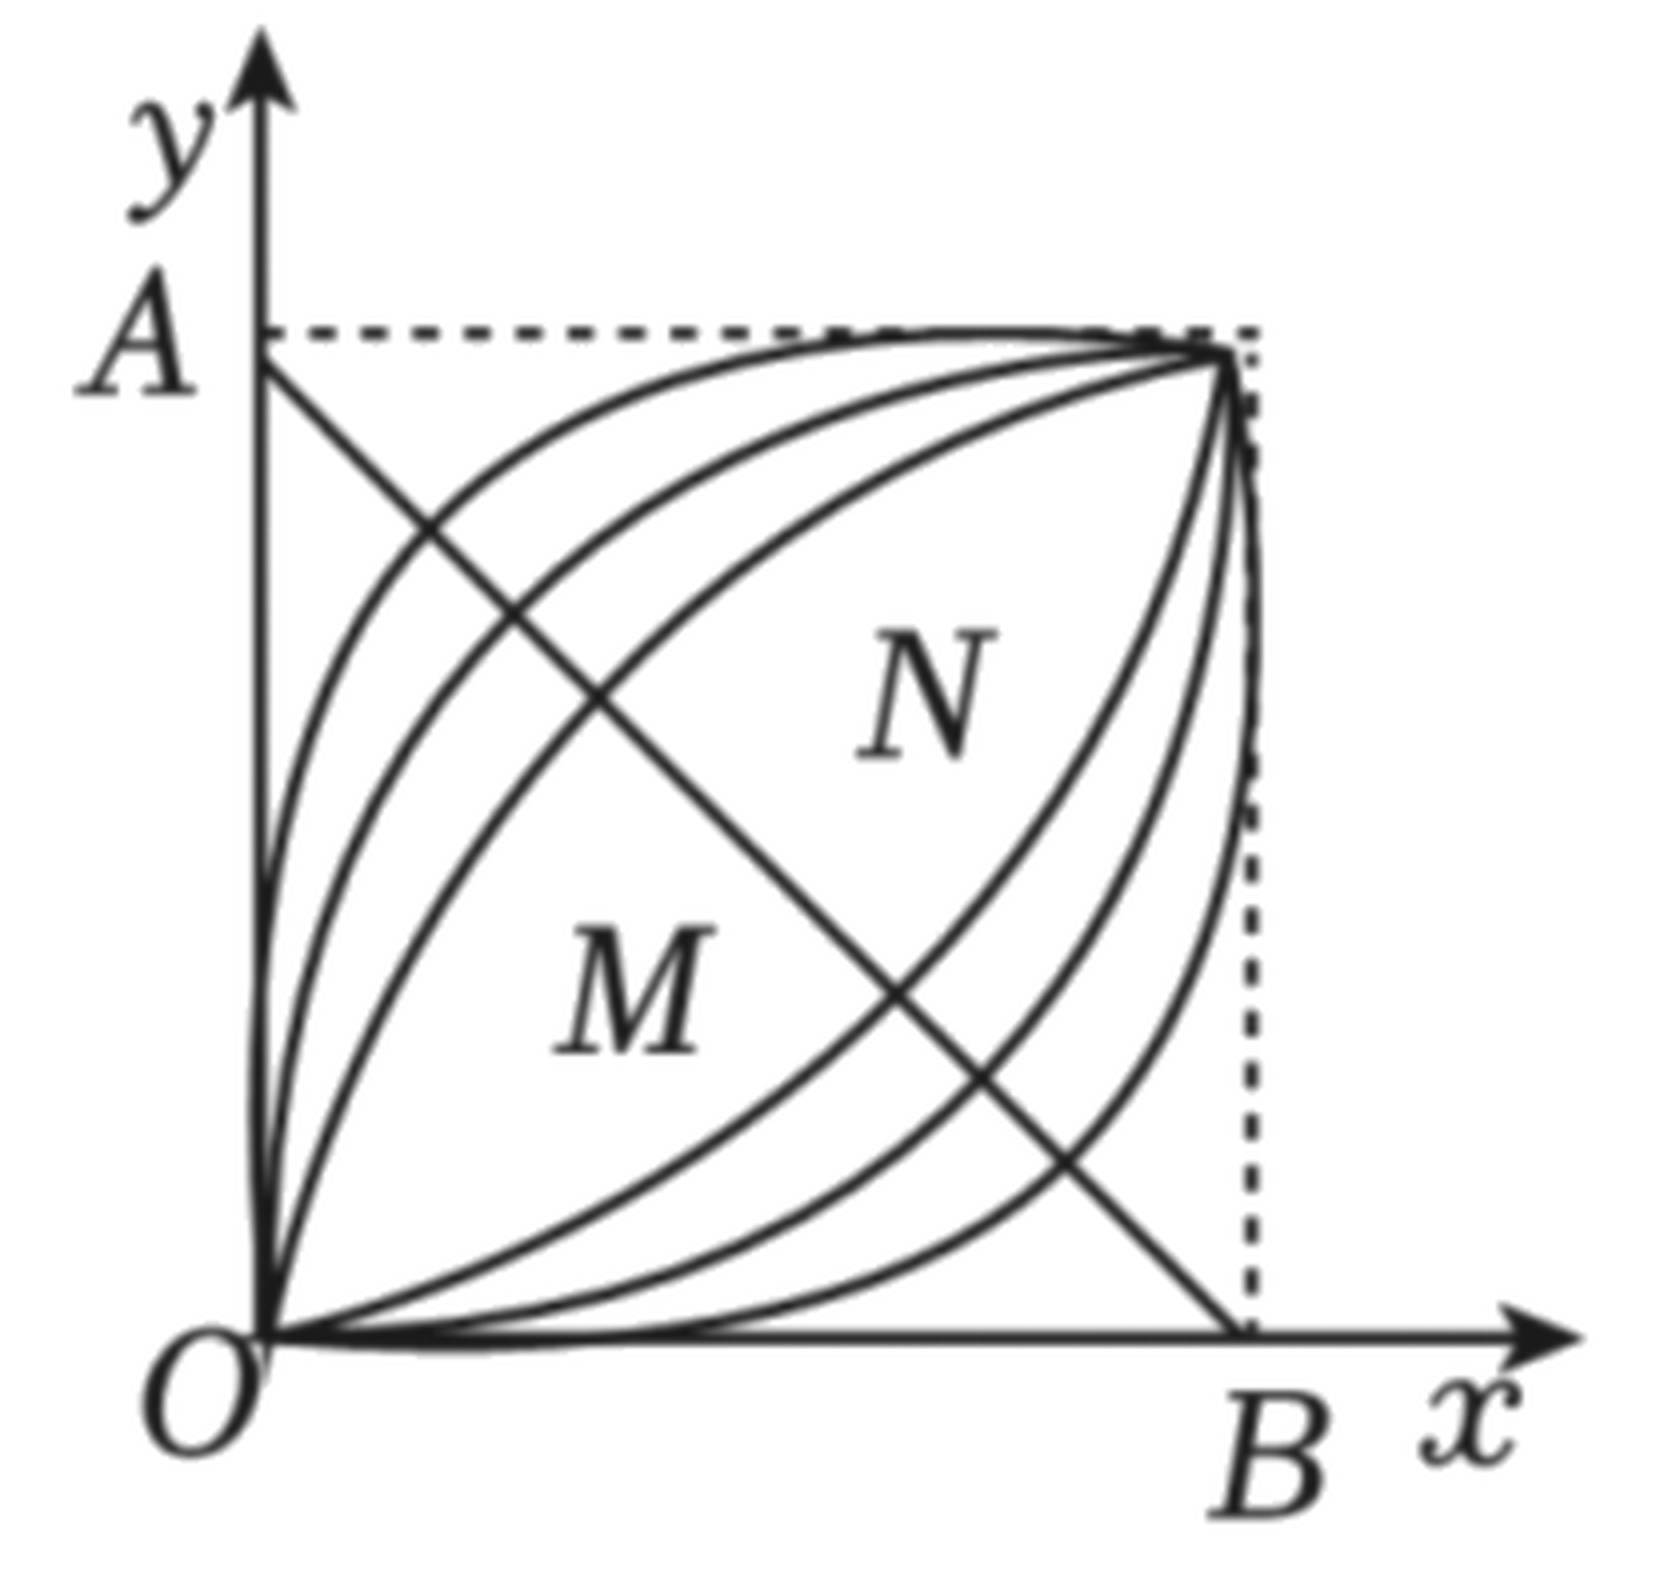
\includegraphics[width=0.40\textwidth]{figures/gao148_q12.png}
\end{center}

\ifanswer
\solbegin
\step{$BM=MN=NA$，点 $A(1,0)$，$B(0,1)$，所以 $M\left(\dfrac{1}{3},\dfrac{2}{3}\right)$，$N\left(\dfrac{2}{3},\dfrac{1}{3}\right)$，}
\step{分别代入 $y=x^\alpha$，$y=x^\beta$，$\alpha=\log_{\frac{2}{3}}\dfrac{1}{3},\beta=\log_{\frac{1}{3}}\dfrac{2}{3}$，$\alpha\beta=\log_{\frac{1}{3}}\dfrac{2}{3}\cdot\log_{\frac{2}{3}}\dfrac{1}{3}=1$.}
\solend
\fi

\end{enumerate}

\bigsec{二、选择题}

\begin{enumerate}
\setcounter{enumi}{12}

% === Q13 ===：答案"C"直接印在题干括号内、全卷无该题【答案】/【解析】段，按 高一84 Q13 成例括号留空、另提 \ans{$C$}；弯引号含空格
\item 若 $x$、$y\in\R$，则 “ $x=0$ ” 是 “ $xy=0$ ” 的\mbox{（\quad）}

\keepwithprev
A. 充要条件\qquad\qquad B. 必要不充分条件

C. 充分不必要条件\qquad\qquad D. 既不充分也不必要条件

\ifanswer
\ans{$C$}
\fi

% === Q14 ===：六个结论（圈数字在文本模式）、四选项一行；解析 8 行（对② 的两行公式各占一印刷行）
\item 若 $a<b<0$，下面有六个结论：① $a^2>b^2$；② $a^3<b^3$；③ $\dfrac{1}{a}<\dfrac{1}{b}$；④ $\dfrac{a}{b}>1$；⑤ $\dfrac{1}{a-b}>\dfrac{1}{a}$；⑥ $\lvert a\rvert>-b$. 其中正确的个数是\mbox{（\quad）}

\keepwithprev
A. 1\qquad\qquad B. 2\qquad\qquad C. 3\qquad\qquad D. 4

\ifanswer
\solbegin
\step{对①：$a^2-b^2=(a+b)(a-b),a+b<0,a-b<0$，故 $a^2-b^2>0$，正确；}
\step{对②：$a^3-b^3=(a-b)(a^2+ab+b^2)=(a-b)\left[\left(a+\dfrac{1}{2}b\right)^2+\dfrac{3}{4}b^2\right],a-b<0$，}
\step{$\left(a+\dfrac{1}{2}b\right)^2+\dfrac{3}{4}b^2>0$，故 $a^3-b^3<0$，正确；}
\step{对③：取 $a=-2,b=-1$，则 $\dfrac{1}{a}=-\dfrac{1}{2},\dfrac{1}{b}=-1,\dfrac{1}{a}>\dfrac{1}{b}$，错误；}
\step{对④：$\dfrac{a}{b}-1=\dfrac{a-b}{b},a-b<0,b<0$，故 $\dfrac{a}{b}-1>0$，正确；}
\step{对⑤：取 $a=-2,b=-1$，则 $\dfrac{1}{a-b}=-1,\dfrac{1}{a}=-\dfrac{1}{2},\dfrac{1}{a-b}<\dfrac{1}{a}$，错误；}
\step{对⑥：要证 $\lvert a\rvert>-b$，即 $-a>-b$，即 $a<b$，正确；}
\step{故选 $D$.}
\solend
\fi

% === Q15 ===：题目配图（四条指数函数曲线，三版都出），\needvspace 守卫放 \item 之前；"图象"照录；解析 5 行
\needvspace{8cm}
\item 如图，曲线①②③④分别是指数函数 $y=a^x$，$y=b^x$，$y=c^x$，$y=d^x$ 的图象，则实数 $a$、$b$、$c$、$d$ 的大小关系为\mbox{（\quad）}

\keepwithprev
A. $a<b<c<d$\qquad B. $b<a<d<c$\qquad C. $d<c<b<a$\qquad D. $c<d<a<b$

\begin{center}
% 四条指数函数曲线图取 04 页右侧，去粉色水印、去色、4× LANCZOS 放大；三版都出
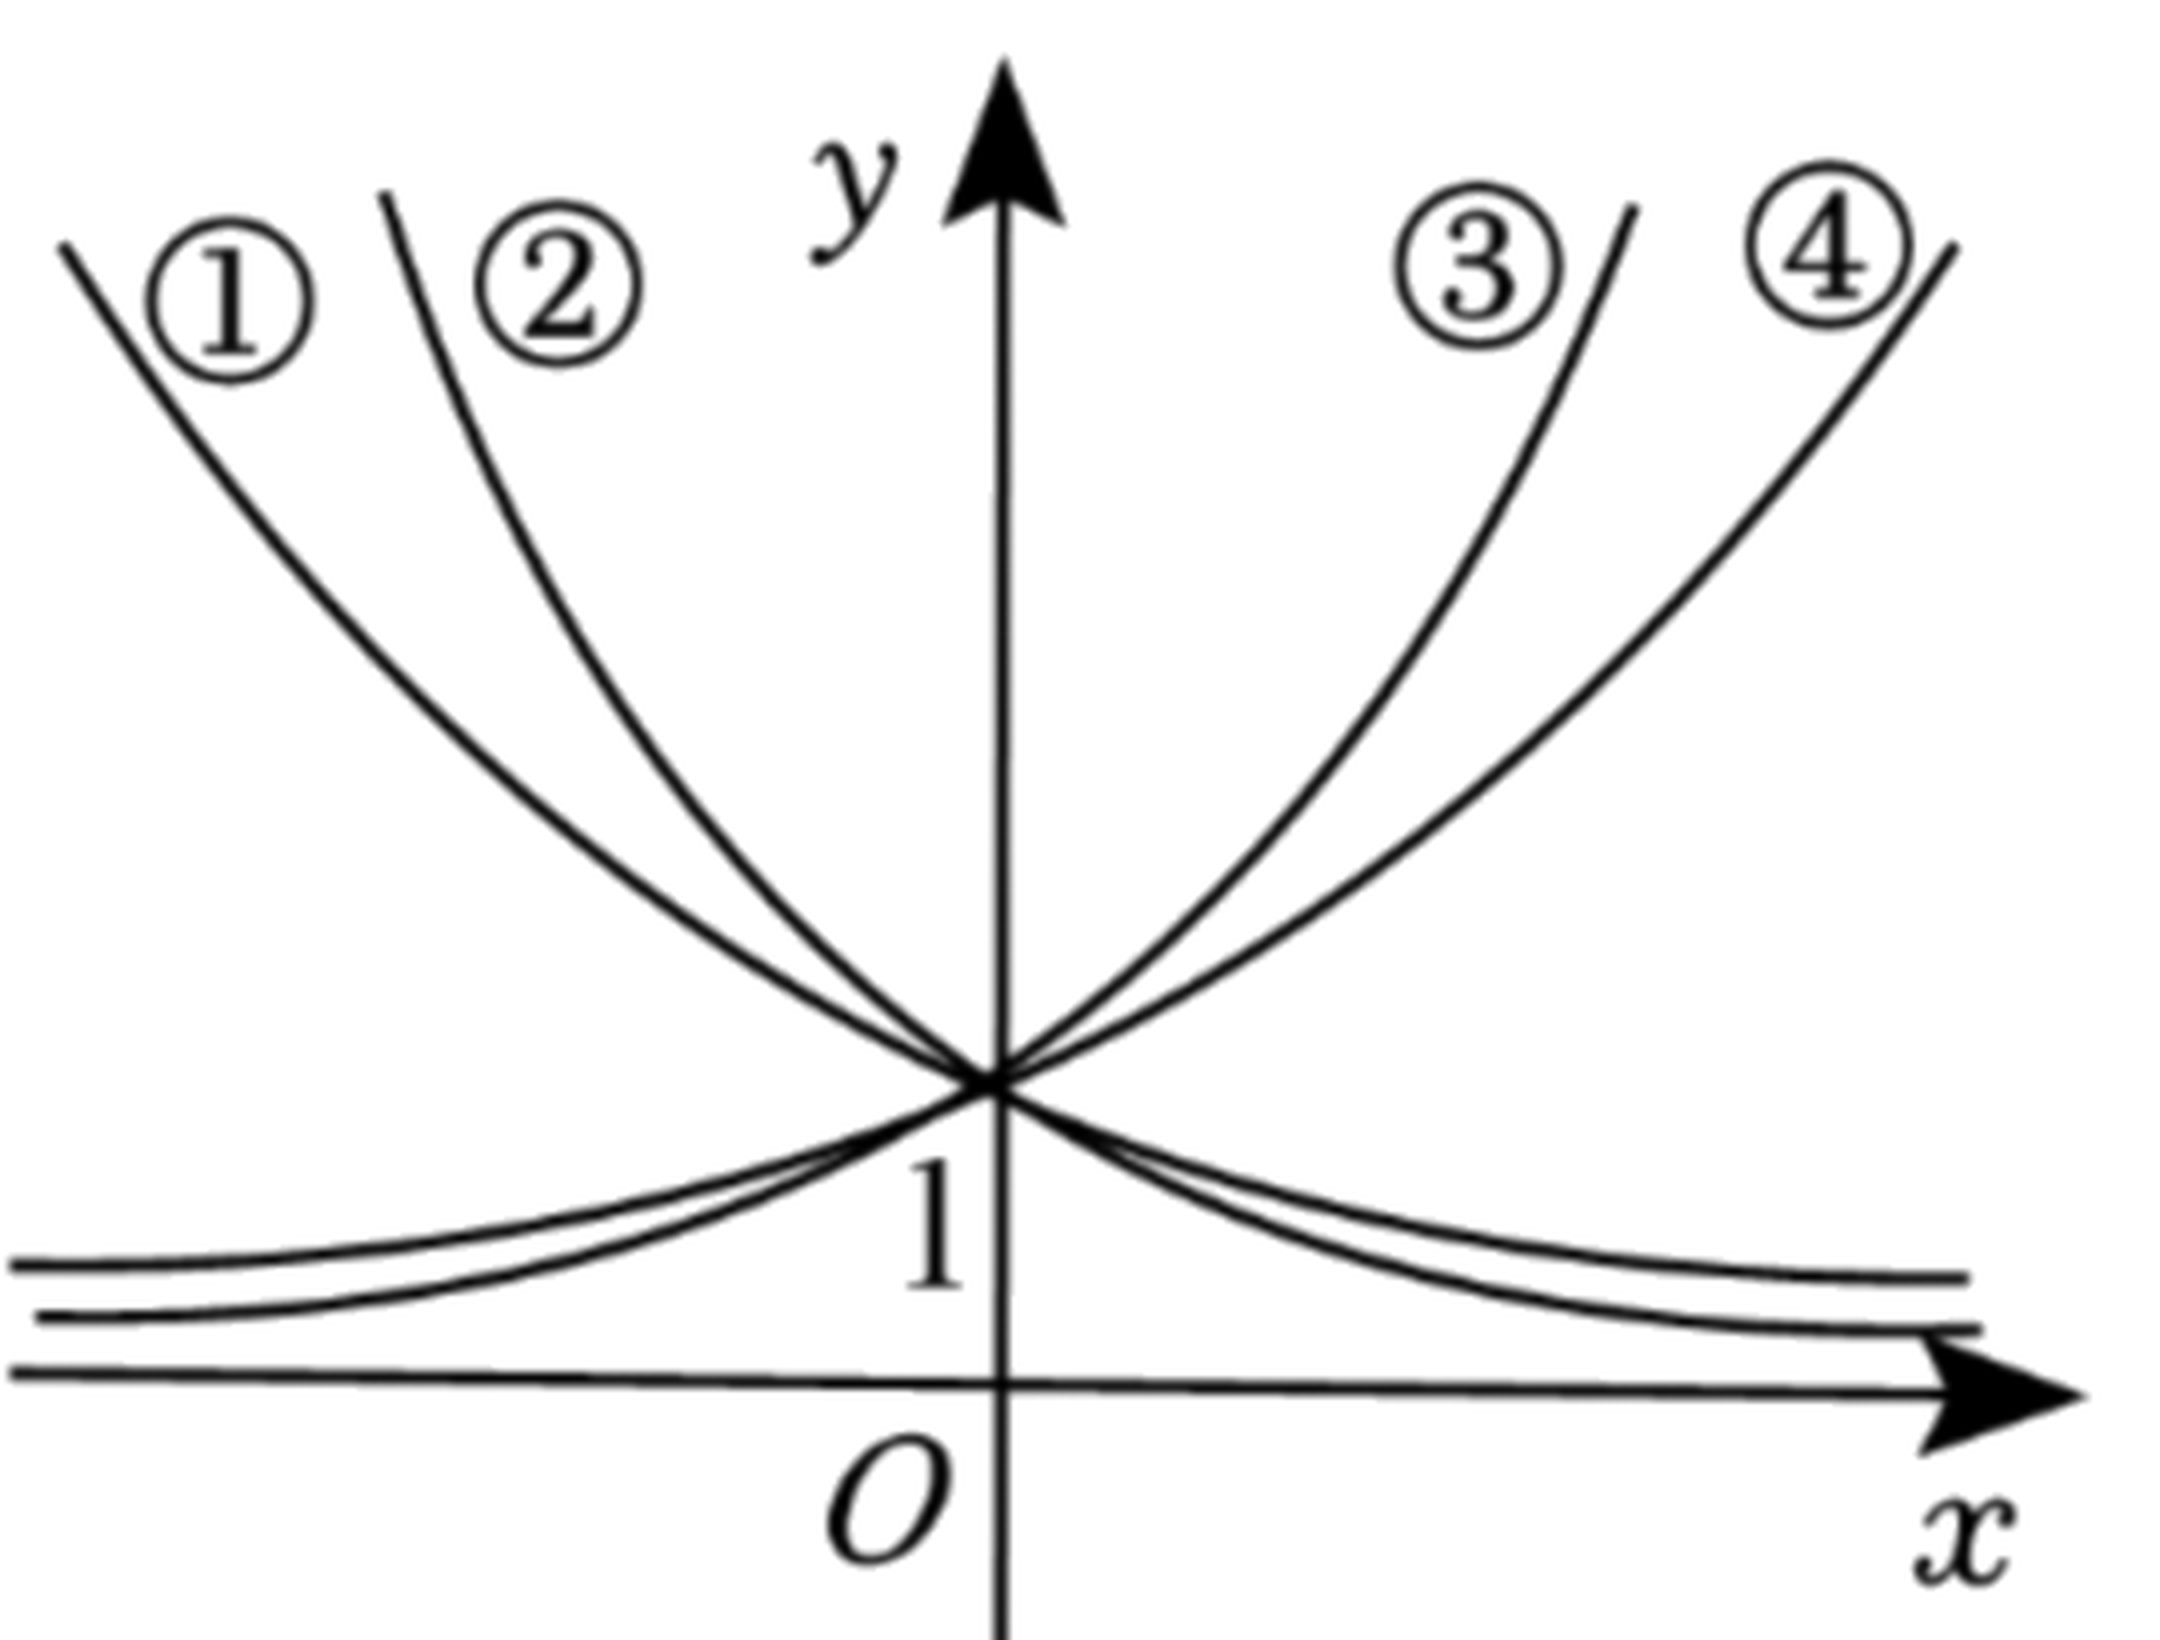
\includegraphics[width=0.40\textwidth]{figures/gao148_q15.png}
\end{center}

\ifanswer
\solbegin
\step{由函数图象得函数① $y=a^x$；② $y=b^x$ 为减函数，且 $x=1$ 时，$b^1<a^1$，}
\step{所以 $0<b<a<1$，}
\step{由函数图象得函数③ $y=c^x$；④ $y=d^x$ 为增函数，且 $x=1$ 时，$c^1>d^1$，}
\step{所以 $c>d>1$，}
\step{所以 $b<a<d<c$. 故选 $B$.}
\solend
\fi

% === Q16 ===：题目配图（关于 y 轴对称的幂函数曲线，三版都出），\needvspace 守卫放 \item 之前；$p$、$q\in\Z$；"图象"照录；解析 2 行
\needvspace{8cm}
\item 已知幂函数 $y=x^{\frac{p}{q}}$（$p$、$q\in\Z$ 且 $p$、$q$ 互质）的图象关于 $y$ 轴对称，如图所示，则\mbox{（\quad）}

\keepwithprev
A. $p$、$q$ 均为奇数，且 $\dfrac{p}{q}>0$\qquad\qquad B. $q$ 为偶数，$p$ 为奇数，且 $\dfrac{p}{q}<0$

C. $q$ 为奇数，$p$ 为偶数，且 $\dfrac{p}{q}>0$\qquad\qquad D. $q$ 为奇数，$p$ 为偶数，且 $\dfrac{p}{q}<0$

\begin{center}
% 关于 y 轴对称的幂函数曲线图取 04 页右下，去粉色水印、去色、4× LANCZOS 放大；三版都出
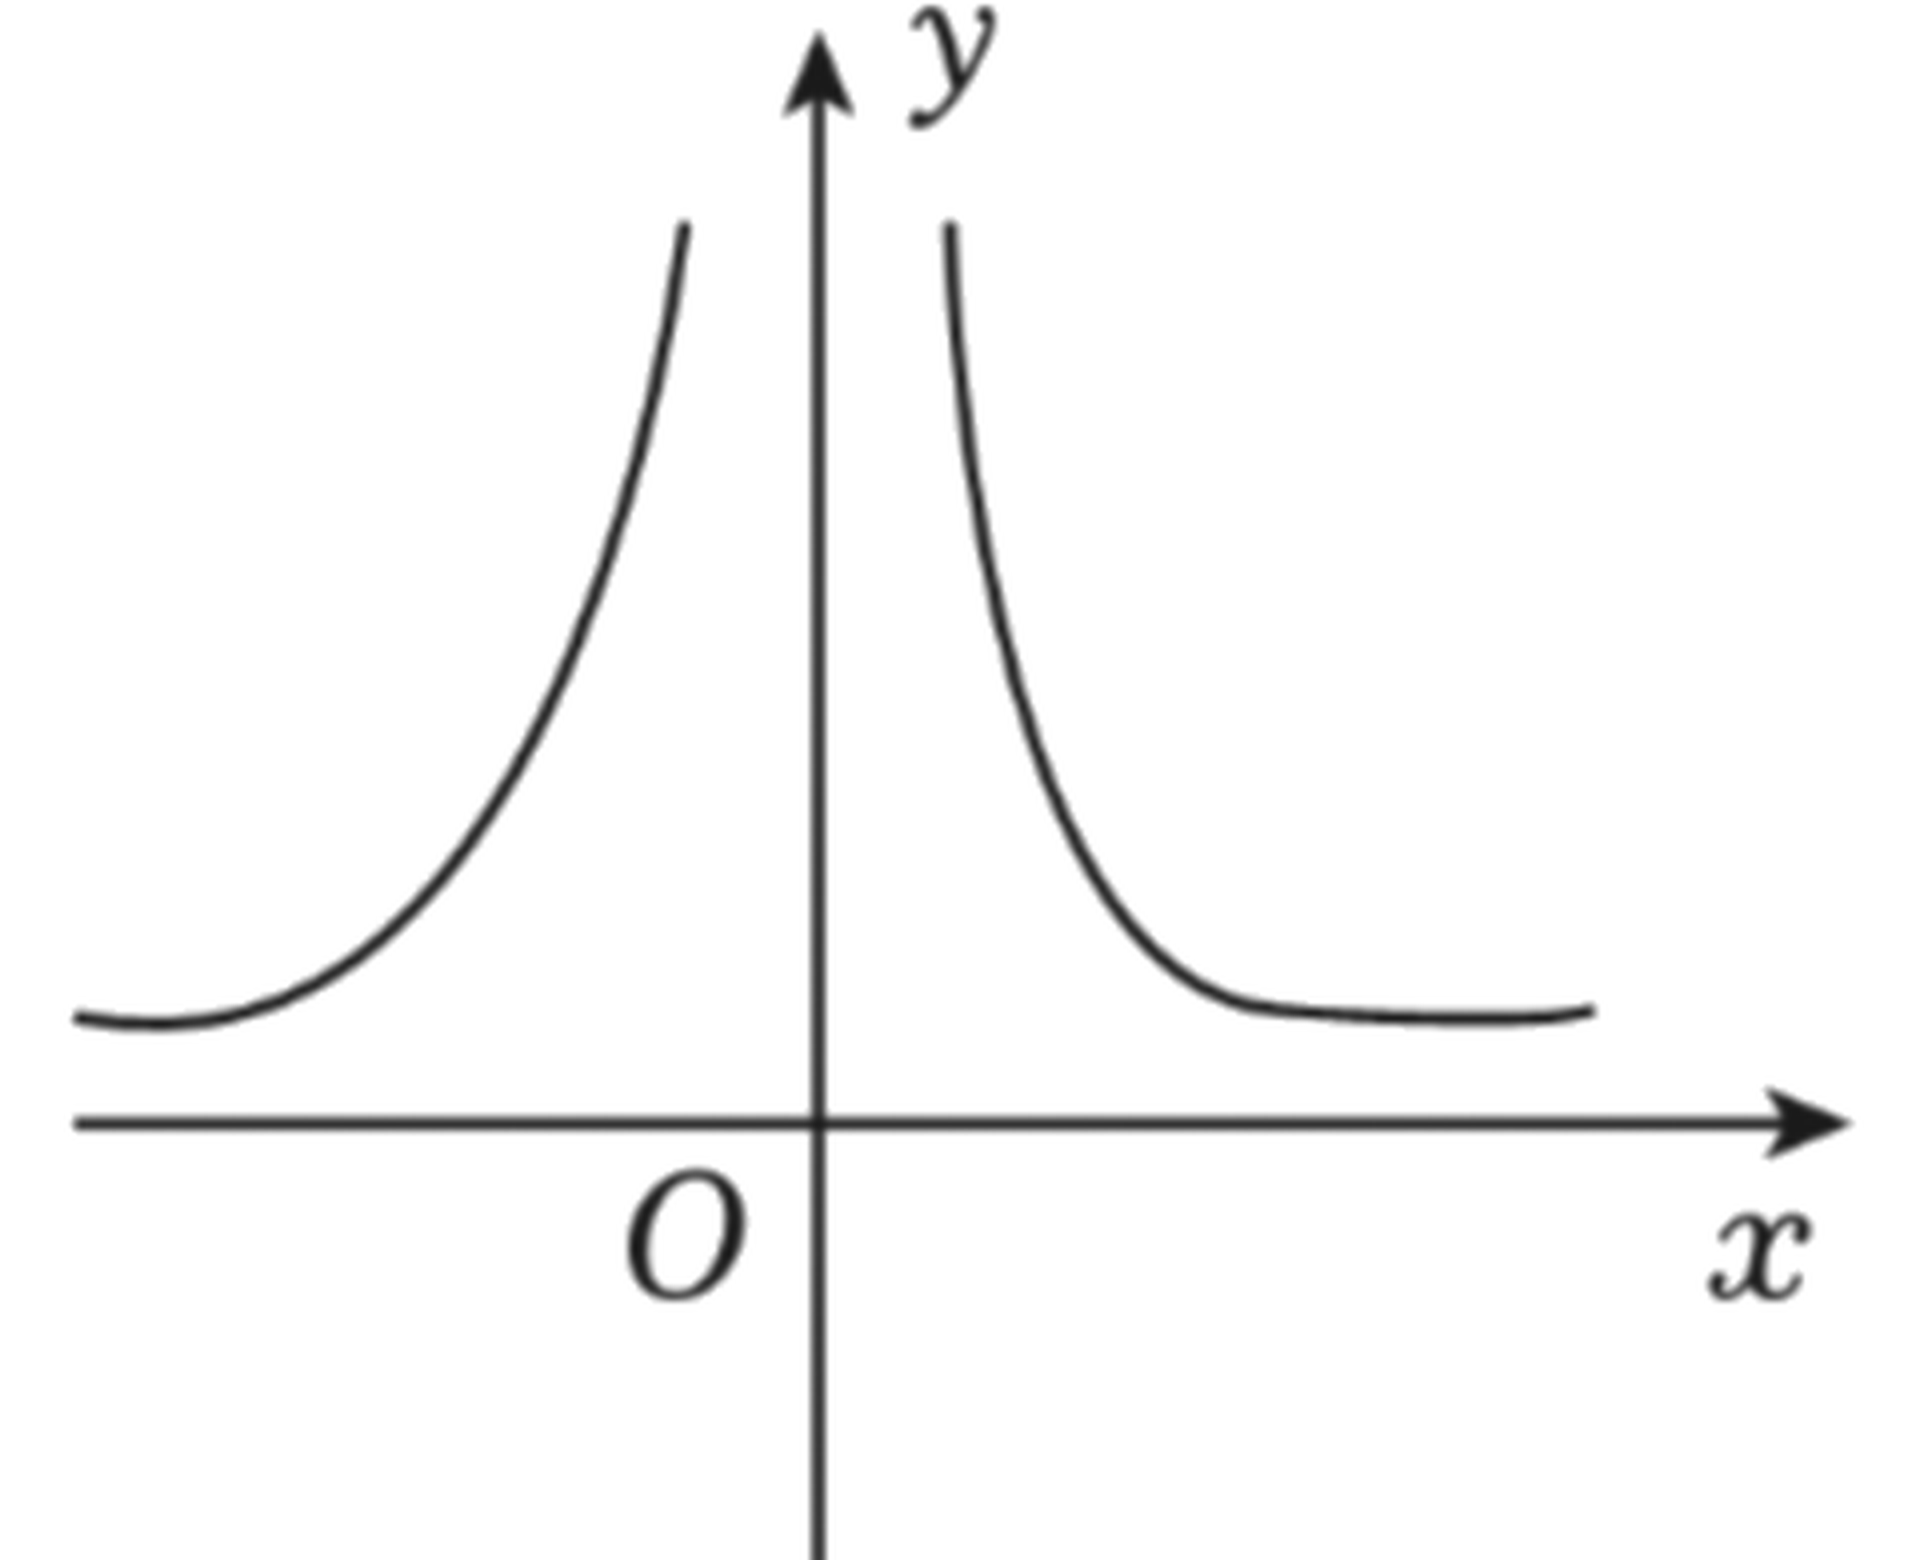
\includegraphics[width=0.36\textwidth]{figures/gao148_q16.png}
\end{center}

\ifanswer
\solbegin
\step{因为函数为偶函数，所以 $p$ 为偶数，且由图象形状判定 $\dfrac{p}{q}<0$.}
\step{又 $p$、$q$ 互质，所以 $q$ 为奇数. 故选 $D$.}
\solend
\fi

\end{enumerate}

\bigsec{三、解答题}

\begin{enumerate}
\setcounter{enumi}{16}

% === Q17 ===：\overline{B}／\varnothing／\R／\mid 逐处照录；解析 8 行
\item 已知集合 $A=\left\{x\mid \dfrac{5}{2x+1}>1\right\}$，$B=\{x\mid x^2+(a+3)x+3a<0,a\in\R\}$.

(1) 求 $A$.

(2) 若全集 $U=\R$，且 $A\cap\overline{B}=\varnothing$，求实数 $a$ 的取值范围.

\ifanswer
\solbegin
\step{(1) $\dfrac{5}{2x+1}>1$，即 $\dfrac{5}{2x+1}-1>0$，即 $\dfrac{4-2x}{2x+1}>0$，即 $(2x+1)(x-2)<0$，}
\step{解得 $-\dfrac{1}{2}<x<2$，所以 $A=\left(-\dfrac{1}{2},2\right)$；}
\step{(2) $x^2+(a+3)x+3a<0$，即 $(x+3)(x+a)<0$，}
\step{全集 $U=\R$，且 $A\cap\overline{B}=\varnothing$，}
\step{当 $a<3$ 时，解得 $-3<x<-a$，则 $\overline{B}=(-\infty,-3)\cup(-a,+\infty)$，}
\step{此时 $-a\geqslant2$，解得 $a\leqslant-2$，}
\step{当 $a\geqslant3$ 时，不满足 $A\cap\overline{B}=\varnothing$，}
\step{故实数 $a$ 的取值范围是 $(-\infty,-2]$.}
\solend
\fi

% === Q18 ===：cases 块整体算一个印刷行；解析 6 行
\item 已知幂函数经过点 $(2,4)$.

(1) 当 $x=\dfrac{1}{2}$ 时，求函数的值；

(2) 是否存在实数 $m$、$n$，使得该函数在区间 $[m,n]$ 上最小值为 $6m-8$，最大值为 $6n-8$？若存在，求出 $m$、$n$ 的值，若不存在，请说明理由.

\ifanswer
\solbegin
\step{(1) 设幂函数的解析式是 $y=x^\alpha$，则 $2^\alpha=4$，解得 $\alpha=2$，}
\step{故 $f(x)=x^2$，$f\left(\dfrac{1}{2}\right)=\dfrac{1}{4}$；}
\step{(2) 因为 $f(x)\geqslant0$，所以 $6m-8\geqslant0$，$m\geqslant\dfrac{4}{3}$，}
\step{由函数 $f(x)$ 在 $(0,+\infty)$ 严格增，得函数 $f(x)$ 在 $(m,n)$ 严格增，}
\step{所以 $\begin{cases}f(m)=6m-8\\f(n)=6n-8\end{cases}$ 且 $m<n$，解得 $m=2$，$n=4$，}
\step{故存在 $m=2$，$n=4$ 满足题意.}
\solend
\fi

% === Q19 ===：7 处评分档照 高一54／64 成例排 \dots\dots N 分；判别式高 \Delta；解析 9 行
\item 已知方程 $x^2+6mx+9m-2=0$，且 $x_1,x_2$ 是方程的两个不同的实数根.

(1) 若 $m=1$，求 $\dfrac{1}{x_1}+\dfrac{1}{x_2}$ 的值；

(2) 若 $m\in\R$，且 $x_1^2+x_2^2<4$，求 $m$ 取值范围.

\ifanswer
\solbegin
\step{(1) 当 $m=1$ 时，方程为 $x^2+6x+7=0$，\dots\dots1 分}
\step{则 $x_1+x_2=-6,x_1\cdot x_2=7$，\dots\dots2 分}
\step{$\dfrac{1}{x_1}+\dfrac{1}{x_2}=\dfrac{x_1+x_2}{x_1\cdot x_2}=-\dfrac{6}{7}$\dots\dots3 分}
\step{(2) $x_1+x_2=-6m,x_1\cdot x_2=9m-2$\dots\dots2 分}
\step{因为 $x_1^2+x_2^2=(x_1+x_2)^2-2x_1\cdot x_2$，所以 $(x_1+x_2)^2-2x_1\cdot x_2<4$，}
\step{所以 $36m^2-2(9m-2)<4$，解得 $0<m<\dfrac{1}{2}$\dots\dots2 分}
\step{又因为方程有两个不同的根，所以 $\Delta=36m^2-4(9m-2)>0$，}% 判别式原卷印等腰偏高粗三角 $\Delta$，照录（放大 07 页 q19_delta3.png／diag_band_q19.png 确认）
\step{解得 $m<\dfrac{1}{3}$ 或 $m>\dfrac{2}{3}$\dots\dots2 分}
\step{所以 $0<m<\dfrac{1}{3}$\dots\dots2 分}
\solend
\fi

% === Q20 ===：题目配图（矩形蔬菜温室，三版都出），\needvspace 守卫放 \item 之前；单位 \mathrm{m}／\mathrm{m}^2；解析 10 行
\needvspace{8cm}
\item 某村计划建造一个室内面积为 $600\mathrm{m}^2$ 的矩形蔬菜温室，在室内，沿左、右两侧与后侧内墙各保留 $2\mathrm{m}$ 宽的通道，沿前侧内墙保留 $4\mathrm{m}$ 宽的空地.

\begin{center}
% 矩形蔬菜温室示意图取 07 页右侧，去粉色水印、去色、4× LANCZOS 放大；三版都出
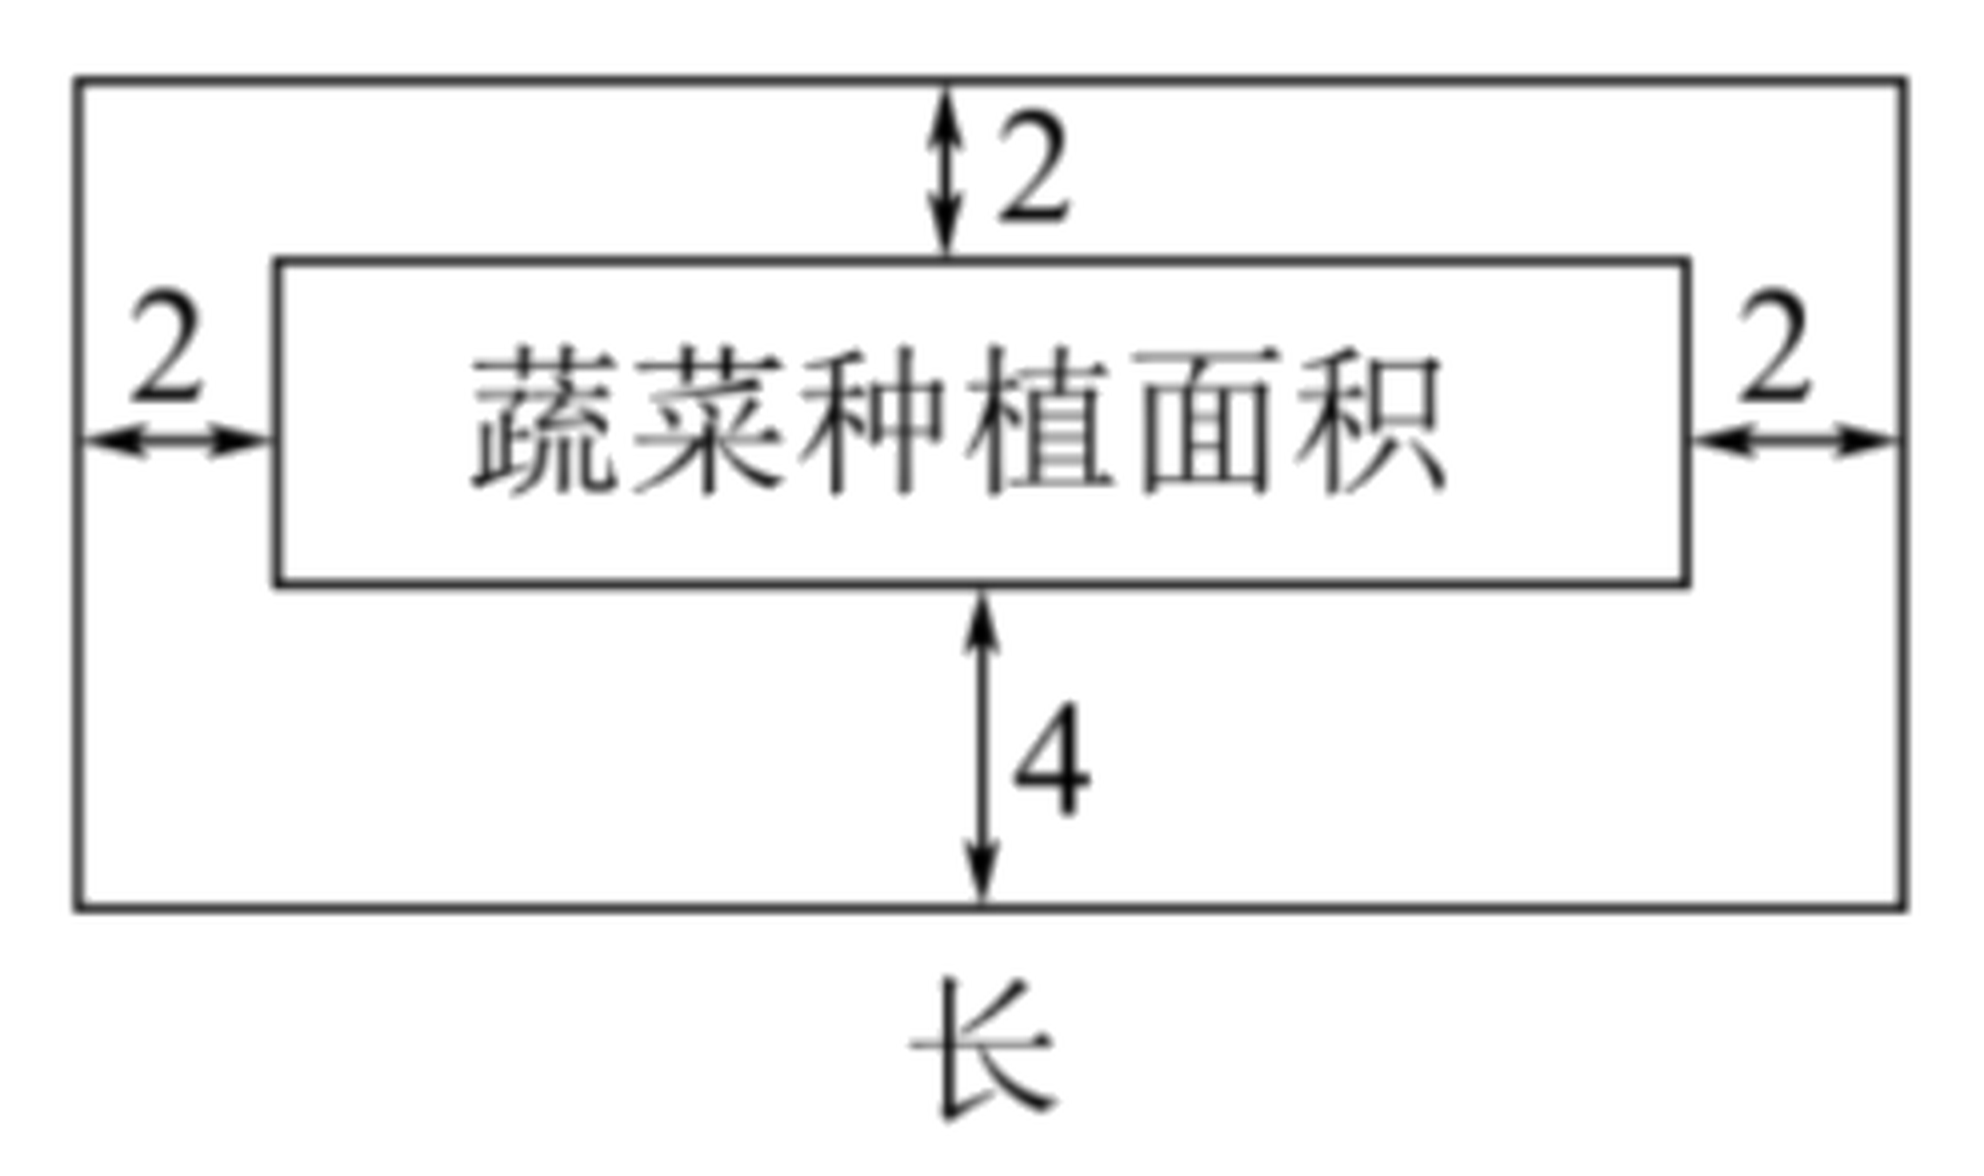
\includegraphics[width=0.45\textwidth]{figures/gao148_q20.png}
\end{center}

(1) 写出蔬菜的种植面积关于矩形温室的长之间的关系式.

(2) 当矩形温室的边长各为多少时，蔬菜的种植面积最大？最大种植面积是多少？

\ifanswer
\solbegin
\step{(1) 设蔬菜的种植面积为 $y\mathrm{m}^2$，矩形温室的长为 $x\mathrm{m}$，}
\step{则矩形温室的宽为 $\dfrac{600}{x}\mathrm{m}$，}
\step{种植蔬菜矩形的长为 $(x-4)\mathrm{m}$，宽为 $\left(\dfrac{600}{x}-6\right)\mathrm{m}$，}
\step{所以 $y=(x-4)\left(\dfrac{600}{x}-6\right)(4<x<100)$；}
\step{(2) 因为 $y=(x-4)\left(\dfrac{600}{x}-6\right)=624-\left(6x+\dfrac{2400}{x}\right)$，}
\step{因为 $6x+\dfrac{2400}{x}\geqslant2\sqrt{6x\cdot\dfrac{2400}{x}}=240$，}
\step{当且仅当 $6x=\dfrac{2400}{x}$，即 $x=20$ 时取等号，}
\step{所以 $y=624-\left(6x+\dfrac{2400}{x}\right)\leqslant624-240=384$.}
\step{即当矩形温室的一边长为 $20\mathrm{m}$，另一边长为 $30\mathrm{m}$ 时，}
\step{蔬菜的种植面积最大，最大为 $384\mathrm{m}^2$.}
\solend
\fi

% === Q21 ===：3 问、cases 块整体算一个印刷行；判别式高 \Delta；解析 19 行（末行续 09 页）
\item 二次函数 $f(x)=ax^2+bx+c$ 满足对任意的 $x\in\R$，$x-1\leqslant f(x)\leqslant x^2-x$ 恒成立.

(1) 求证：$f(1)$ 为定值；

(2) 若 $f(0)=-\dfrac{1}{4}$，求二次函数 $f(x)$ 的表达式；

(3) 求 $a+2b+5c$ 的取值范围.

\ifanswer
\solbegin
\step{(1) 对任意的 $x\in\R$，$x-1\leqslant f(x)\leqslant x^2-x$ 恒成立，则 $0\leqslant f(1)\leqslant0$，}
\step{所以 $f(1)=0$，为定值.}
\step{(2) 由(1)得 $a+b+c=f(1)=0$，由 $f(0)=-\dfrac{1}{4}$，得 $c=-\dfrac{1}{4}$，}
\step{则 $b=\dfrac{1}{4}-a$，$f(x)=ax^2+\left(\dfrac{1}{4}-a\right)x-\dfrac{1}{4}$，}
\step{不等式 $x-1\leqslant f(x)$ 可化为 $ax^2+\left(\dfrac{1}{4}-a\right)x-\dfrac{1}{4}\geqslant x-1$，}
\step{即 $ax^2-\left(a+\dfrac{3}{4}\right)x+\dfrac{3}{4}\geqslant0$，}
\step{一元二次不等式 $ax^2-\left(\dfrac{3}{4}+a\right)x+\dfrac{3}{4}\geqslant0$ 恒成立，则 $\begin{cases}a>0\\\Delta=\left(a+\dfrac{3}{4}\right)^2-3a\leqslant0\end{cases}$，}% 判别式原卷印等腰偏高粗三角 $\Delta$，照录（放大 08 页 q21_delta3.png／diag_band_q21.png 确认）
\step{解得 $a=\dfrac{3}{4}$，}
\step{此时 $f(x)=\dfrac{3}{4}x^2-\dfrac{1}{2}x-\dfrac{1}{4}$，$x^2-x-f(x)=\dfrac{1}{4}(x-1)^2\geqslant0$ 恒成立，}
\step{所以 $f(x)=\dfrac{3}{4}x^2-\dfrac{1}{2}x-\dfrac{1}{4}$.}
\step{(3) 由(1)得 $b=-a-c$，$f(x)=ax^2-(a+c)x+c=(ax-c)(x-1)$，}
\step{不等式 $x-1\leqslant f(x)$ 可化为 $(x-1)(ax-c-1)\geqslant0$，}
\step{一元二次不等式 $(x-1)(ax-c-1)\geqslant0$ 恒成立，则 $a>0$，}
\step{且方程 $(x-1)(ax-c-1)=0$ 有相等的实数根，因此 $c=a-1$，$a>0$，}
\step{不等式 $f(x)\leqslant x^2-x\Leftrightarrow(ax-c)(x-1)\leqslant x^2-x\Leftrightarrow(x-1)[(1-a)x+c]\geqslant0$，}
\step{同理 $1-a>0$，且方程 $(x-1)[(1-a)x+c]=0$ 有相等的实数根，}
\step{因此 $c=a-1$，$a<1$，从而 $c=a-1$，$b=1-2a$，$0<a<1$，}
\step{$a+2b+5c=a+2(1-2a)+5(a-1)=2a-3\in(-3,-1)$，}
\step{所以 $a+2b+5c$ 的取值范围是 $(-3,-1)$.}
\solend
\fi

\end{enumerate}

\end{document}
"
% 紧凑版：xelatex "\def\iscompact{1}% 高一148_新川中学_期中.tex
%   —— 高一上数学"2026-2027 年新川中学高一上期中"（试卷版/答案版/紧凑版）
% 试卷版：xelatex 高一148_新川中学_期中.tex
% 答案版：xelatex "\def\isanswer{1}\input{高一148_新川中学_期中.tex}"
% 紧凑版：xelatex "\def\iscompact{1}\input{高一148_新川中学_期中.tex}"
%
% ① 原始材料：微信公众号"魔都数学加油站"文章，连载"27学年高一148"，原文标题
% "27学年高一148——2026-2027年上海市新川中学高一上期中"（2026-11-21 推送）；
% 原文链接：https://mp.weixin.qq.com/s/Alhmwb3sSLQMp_wjzoAVyA 。
% 正文为 9 张 PNG 页（01/03/04/07/08/09 为 2560×3620，02/05/06 为 4762×6735，
% 同一篇各页分辨率混排，逐页按各自分辨率裁图核对，别按预览比例换算裁框）。
% 体例：混合体例讲评版——19 题中 Q4、Q5 只印【答案】、无【解析】；Q13 的答案"C"
% 直接印在题干括号内、无【答案】/【解析】段；其余 16 题印【解析】（逐题核实，见 ② ②）。
% 题目、答案、解析均据原图转录；卷面粉红色水印"魔都数学加油站"及公众号页脚未录入。
% 全卷插图清单（逐页通读 9 页确认）：4 幅题目配图，均三版都出、均非【解析】内配图：
%   · Q12 幂函数曲线族图（03 页右侧：x/y 轴、O、A(1,0)、B(0,1)、M、N 与两族
%     y=x^α／y=x^β 曲线、线段 AB、虚线），题干"（如图）"处，裁 figures/gao148_q12.png；
%   · Q15 四条指数函数曲线图（04 页右侧：①②③④ 四曲线同过 (0,1)、x/y 轴、O、
%     y 轴刻度 1），题干"如图"处，裁 figures/gao148_q15.png；
%   · Q16 关于 y 轴对称的幂函数曲线图（04 页右下：x/y 轴、O、两支上翘曲线），
%     题干"如图所示"处，裁 figures/gao148_q16.png；
%   · Q20 矩形蔬菜温室示意图（07 页右侧：大矩形＋内框"蔬菜种植面积"＋2/2/4
%     通道标注＋"长"），题干处，裁 figures/gao148_q20.png；
%   其余各页逐页确认无其它题目配图、无【解析】内配图、无表格，亦无"题干写如图而
%   源码漏图"一处；Q19 解析行末的虚线"----N 分"为评分档（非图），Q18／Q21 的
%   cases 块为数学块（非图）。4 图均取自原卷截图，去粉色水印、去色、4× LANCZOS 放大。
%
% 卷首标题：原卷印作"2026-2027 年新川中学高一上期中"，年份区间按全稿惯例排 en dash；
% 原卷卷面未印副标题，本稿按同期中卷（高一140／141／143／144／145／146／147）知识模块
% 口径补出"集合与常用逻辑用语、不等式、函数"。
%
% 题号体例（逐页核实定稿）：本卷共 19 题——一、填空题 3—12（10 题）、
% 二、选择题 13—16（4 题）、三、解答题 17—21（5 题）。
% 三节分别 \setcounter{enumi}{2}／{12}／{16}。原卷从第 3 题起、无第 1、2 题，
% 本稿保留原题号；全卷无附加题节、无 Q22（Q21 解析末行"所以 a+2b+5c 的取值范围是
% (-3,-1)."为全卷收尾，09 页下半仅水印、无正文）。
%
% ② 与原卷的排版差异：
%   ① 原文从第 3 题起，本稿保留原题号；共 19 题三节；
%   ② 混合体例逐题核实：Q4（反证法"假设的内容"）、Q5 只印【答案】、无【解析】，
%      按 高一140 第 5 题／高一145 Q3 成例提 \ans{}、不补造解析；Q13 答案"C"直接
%      印在题干括号内（" ( C ) "）、全卷无该题【答案】/【解析】段，按 高一84 Q13／
%      高一37 Q13／高一53 Q13 成例括号 \mbox{（\quad）} 留空、另提 \ans{$C$}；
%      其余 16 题印【解析】、用 \solbegin…\solend，选择题答案在解析末句"故选 X"
%      （Q14 选 D、Q15 选 B、Q16 选 D，逐个放大原图核实）、题干括号留空、不另提
%      \ans{}；答案版【答案】/【解析】标记数 = 19（3 个 \ans ＋ 16 个 \solbegin）
%      = 全卷题数；
%   ③ 原卷卷面未印副标题，本稿按知识模块口径补出；
%   ④ 原卷填空横线按全稿惯例排 \blankline[4.4em]；选择题括号排 \mbox{（\quad）}、
%      选项段前按惯例加 \keepwithprev；Q13／Q16 四选项为两行两列、Q14／Q15 选项
%      为一行，照原卷分行；解答题不留作答区、不加 \anspace（原卷为讲评版，
%      与 129／131／132／133／136／140／141／143／144／145／146 同）；
%   ⑤ 数集：Q11"在 R 上定义运算"、Q13"x、y∈R"、Q16"p、q∈Z"、Q17"a∈R"
%      "U=R"、Q19"m∈R"、Q21"x∈R" 原卷印斜体 R/Z，按全稿惯例统一改 \R／\Z
%      （本卷未出现 N，\N^* 无对应处）；绝对值排 \lvert…\rvert（Q9／Q14），
%      集合描述竖线排 \mid（Q17）；不等号按全稿惯例排 \leqslant／\geqslant；
%      补集照原卷上划线排 \overline{B}（Q17 题干 1 处＋解析 3 处）；空集
%      \varnothing（Q17 题干 1 处＋解析 2 处）；\subset（Q3 题干 {a}⊂M）与
%      \subseteq（Q3 题干 M⊆{a,b,c,d}）逐处照录不统一（放大 01 页 q3_subset.png）；
%   ⑥ 子题标号 (1)(2)(3) 半角括号照录；圈数字 ①—⑥ 在文本模式（Q14 六个结论、
%      Q15 曲线编号与其解析、Q14 解析"对①…对⑥"），按 common.sty 划入 CJK 字符类
%      渲染；cases 块整体算一个印刷行；\left…\right 不得拆到不同 $…$ 组；
%      单位 m／m² 排 \mathrm{m}／\mathrm{m}^2（Q20，原卷印正体 m）；
%   ⑦ 题干／解析中的中文弯引号按原卷照录：Q4" ab 可以被 5 整除，那么 a、b 中
%      至少有一个能被 5 整除 "（开引号后有空格、闭引号后空格接"时"）、
%      Q13" x=0 "" xy=0 "（引号内空格），注释内一律 ASCII 引号；
%   ⑧ 半角逗号在数学组之间是全稿惯例、非笔误（Q3"{a,b,c,d}"、Q6"$x,y$"
%      "$x=\frac13,y=\frac16$"、Q10、Q11"$a=-2,b=-1"、Q12"$\alpha=\log..,\beta=..$"、
%      Q14"$a+b<0,a-b<0$"、Q17、Q19"$x_1+x_2=-6,x_1\cdot x_2=7$"、Q20、Q21 等），
%      逐处照录别改全角；行末西文句点照录为 ASCII `.`；行中全角逗号／顿号照录；
%   ⑨ "图像／图象"逐处放大核：全卷 9 处均印"图象"（象，无亻）、未见"图像"，
%      逐处照录未统一改动（Q8 题干/解析各 1、Q12 题干 2、Q15 题干 1／解析 2、
%      Q16 题干 1／解析 1；放大 02/03/04/05 页 /tmp/gao148/zoom/my_wide_a.png、
%      my_wide_b.png 与宋体参考"象／像"并排确认）；
%   ⑩ 判别式 Δ/△ 混用是照录项：Q11 解析"△=1−4(−a²+a+1)<0"印扁等边空心
%      三角 \triangle；Q19 解析"Δ=36m²−4(9m−2)>0"、Q21 解析 cases 块
%      "Δ=(a+3/4)²−3a≤0" 两处印等腰偏高粗三角 \Delta，逐处放大判断、照录
%      不统一（参照 高一142／144／145 头注④口径，详见 ④）；
%   ⑪ 一条 \step = 原卷解析的一个印刷行，cases 块整体算一个印刷行；别把原卷折行
%      并起来、别把一行拆多条。Q3 六行、Q7 五行（01 页末首行＋02 页顶四行）、
%      Q9 七行、Q11 五行、Q14 八行（对② 的两行公式各占一印刷行）、Q17 八行、
%      Q18 六行、Q19 九行（7 处评分档附在行末）、Q20 十行、Q21 十九行
%      均按印刷行逐条断，不丢行；
%   ⑫ 配图：4 幅均为题目配图（三版都出），放 \item 内题干之后 \begin{center}；
%      大图块加 \needvspace 守卫把整块推走（守卫放 \item 之前，见 高一145 Q14/Q20
%      成例与切页审计 B 类坑）；三版切页审计均"合计异常：无"；
%   ⑬ 跨页续印按题合并：Q3/4/5 在 01 页；Q6 题干＋解析在 01 页；Q7 题干在 01 页
%      末、解析首行在 01 页末续 02 页顶四行；Q8/9/10 在 02 页（Q9 解析续 02 页下半、
%      Q10 题干与解析前 2 行在 02 页末）；Q10 解析末行续 03 页顶；Q11/12 在 03 页、
%      "二、选择题"标题与 Q13/14 题干在 03 页下半；Q13 无解析；Q14 解析在 04 页顶、
%      Q15 题干＋图＋选项＋解析在 04 页、Q16 题干＋图在 04 页末；Q16 选项＋解析＋
%      "三、解答题"标题＋Q17 题干＋解析在 05 页、Q18 题干首句在 05 页末；Q18 题干
%      续＋解析、Q19 题干＋解析前 5 行在 06 页；Q19 解析续 4 行＋Q20 题干＋图＋
%      解析（10 行全部）在 07 页，末行"蔬菜的种植面积最大，最大为 384m²."收尾；
%      Q21 题干＋解析前 18 行在 08 页；Q21 解析末行"所以 a+2b+5c 的取值范围是
%      (-3,-1)."在 09 页上半（09 页下半仅水印、无正文）。本稿按题连排，不丢行、
%      不并折行；
%   ⑭ 原卷解析内无红色"法一／法二"之类小标题，故本卷无 \stepm；水印
%      "魔都数学加油站"红色不录入；Q19 解析 7 处评分档（1/2/3/2/2/2/2 分）
%      原卷在行末印一串虚线，本稿照 高一54／64 成例排 \dots\dots N 分，
%      分值逐处照录、位置不变。
%
% ③ 行数复核：一条 \step／\stepm = 原卷解析的一个印刷行，cases 块作一个印刷行计。
%   逐题数（主会话逐页核对定稿）：Q3：6；Q4：0（只印【答案】、提 \ans{}）；
%   Q5：0（只印【答案】、提 \ans{}）；Q6：2；Q7：5；Q8：2；Q9：7；Q10：3；
%   Q11：5；Q12：2；Q13：0（答案印在题干括号内、另提 \ans{}）；Q14：8；Q15：5；
%   Q16：2；Q17：8；Q18：6；Q19：9；Q20：10；Q21：19。
%   合计 99 条 \step（本卷无 \stepm：解析内无红色"法一／法二"类小标题），
%   与原卷逐题印刷行相等。全卷 16 题设 \solbegin…\solend ＋ 3 处 \ans{}，
%   答案版【答案】/【解析】标记数 = 19 = 全卷题数。
%
% ④ 判别式／子集符号结论（逐处放大原图照录、不得统一，主会话像素级复核）：
%   判别式全卷 3 处，两形混用逐处照录不统一（参照 高一142／144／145 头注④口径）：
%     · Q11 解析"△=1−4(−a²+a+1)<0" 原卷印扁等边空心三角（宽>高、细线），
%       照录 \triangle（放大 03 页 /tmp/gao148/zoom/q11_delta3.png、
%       delta_montage.png 确认）；
%     · Q19 解析"Δ=36m²−4(9m−2)>0" 原卷印等腰偏高粗三角（高>宽），
%       照录 \Delta（放大 07 页 /tmp/gao148/zoom/q19_delta3.png 确认）；
%     · Q21 解析 cases 块"Δ=(a+3/4)²−3a≤0" 原卷印等腰偏高粗三角（高>宽），
%       照录 \Delta（放大 08 页 /tmp/gao148/zoom/q21_delta3.png 确认）。
%   子集／补集：Q3 题干"{a}⊂M⊆{a,b,c,d}" 前者印单线 ⊂、无下划线，照录 \subset；
%     后者印带下划线 ⊆，照录 \subseteq（放大 01 页 /tmp/gao148/zoom/q3_subset.png
%     确认）；Q17 题干 1 处＋解析 3 处共 4 处 \overline{B} 照原卷上划线
%     （B 上横线、非 C_U B）；空集 \varnothing 3 处（Q17 题干 1 处、解析 2 处）；
%     Q17 集合描述竖线 \mid；数集 \R／\Z 归一见 ② ⑤。
%
% ⑤ 存疑照录（放大原图确认，照录未改、正文对应处另有 % 注）：
%   1. Q3 解析末行"所以 M 一共有 3+3+1+1=8 个" 原卷印 $3+3+1+1=8$，按上文
%      四行应为 $1+3+3+1=8$（疑为原卷加数顺序笔误，和仍为 8），放大 01 页
%      /tmp/gao148/zoom/my_q3_sol.png 确认，照录未改。
%   2. Q13 答案"C"直接印在题干括号内、全卷无该题【答案】/【解析】段，按
%      高一84 Q13 成例括号留空、另提 \ans{$C$}（见 ② ②），未补造解析。
%   3. Q19 解析 7 处评分档（"----N 分"）原卷印一串虚线，本稿照 高一54／64
%      成例排 \dots\dots N 分，分值逐处照录、位置不变。
%   4. 判别式 Q11 扁 \triangle 与 Q19／Q21 高 \Delta 两形混用，逐处照录不统一（见 ④）。
%   5. "图像／图象"全卷 9 处均印"图象"、未见"图像"（见 ② ⑨），逐处放大核实照录，
%      未统一改动。
%   全卷除此 5 类外未发现其它笔误／自相矛盾处。
%
% ⑥ 跨页续印按题合并说明：见 ② ⑬。
%
\documentclass[a4paper,11pt]{article}
\usepackage{common}

\begin{document}

\examtitlest[3]{2026--2027 年新川中学高一上期中}{集合与常用逻辑用语、不等式、函数}

\bigsec{一、填空题}

\begin{enumerate}
\setcounter{enumi}{2}

% === Q3 ===：题干 {a}⊂M⊆{a,b,c,d} 两个子集符号逐处照录；解析 6 行
\item 满足 $\{a\}\subset M\subseteq\{a,b,c,d\}$ 的集合 $M$ 有\blankline[4.4em]个.

\ifanswer
\solbegin
\step{$M$ 是 $\{a,b,c,d\}$ 的子集，但必含有元素 $a$，}
\step{当 $M$ 中只一个元素时，$M=\{a\}$ 只有 1 个；}
\step{当 $M$ 中有二个元素时，$M$ 有 3 个；}
\step{当 $M$ 中有三个元素时，$M$ 有 3 个；}
\step{当 $M$ 中有四个元素时，$M$ 有 1 个；}
\step{所以 $M$ 一共有 $3+3+1+1=8$ 个.}% 原卷印 $3+3+1+1=8$（按上文四行应为 $1+3+3+1$），疑为加数顺序笔误，照录未改（放大 01 页 my_q3_sol.png）
\solend
\fi

% === Q4 ===：原卷只印【答案】、无【解析】，按 高一140 第 5 题成例提 \ans{}；弯引号与空格照录
\item 用反证法证明命题 “ $ab$ 可以被 5 整除，那么 $a$、$b$ 中至少有一个能被 5 整除” 时假设的内容应该是\blankline[4.4em].

\ifanswer
\ans{$a$、$b$ 都不能被 5 整除}
\fi

% === Q5 ===：原卷只印【答案】 $[-2,1)$、无【解析】，提 \ans{}
\item 不等式 $\dfrac{x+2}{x-1}\leqslant0$ 的解集为\blankline[4.4em].

\ifanswer
\ans{$[-2,1)$}
\fi

% === Q6 ===：解析 2 行；半角逗号在数学组之间照录
\item 设 $x,y\in(0,+\infty)$，且 $x+4y=1$，则 $\dfrac{1}{x}+\dfrac{1}{y}$ 的最小值为\blankline[4.4em].

\ifanswer
\solbegin
\step{因为 $\dfrac{1}{x}+\dfrac{1}{y}=(x+4y)\left(\dfrac{1}{x}+\dfrac{1}{y}\right)=5+\dfrac{4y}{x}+\dfrac{x}{y}\geqslant5+2\sqrt{\dfrac{4y}{x}\cdot\dfrac{x}{y}}=9$，}
\step{当且仅当 $\dfrac{4y}{x}=\dfrac{x}{y}$，即 $x=2y$，即 $x=\dfrac{1}{3},y=\dfrac{1}{6}$ 时取等号，故最小值为 9.}
\solend
\fi

% === Q7 ===：题干在 01 页末、解析首行在 01 页末续 02 页顶四行；解析 5 行
\item 若不等式 $x^2+ax+b<0$ 的解集为 $(-3,-1)$，则不等式 $bx^2+ax+1\leqslant0$ 的解集为\blankline[4.4em].

\ifanswer
\solbegin
\step{不等式 $x^2+ax+b<0$ 的解集为 $(-3,-1)$，}
\step{所以方程 $x^2+ax+b=0$ 的两个实数根为 $-3$ 和 $-1$，}
\step{由根与系数的关系得 $a=4$，$b=3$，}
\step{故 $bx^2+ax+1\leqslant0$ 可化为 $3x^2+4x+1\leqslant0$，解得 $-1\leqslant x\leqslant-\dfrac{1}{3}$，}
\step{所求不等式 $bx^2+ax+1\leqslant0$ 的解集为 $\left[-1,-\dfrac{1}{3}\right]$.}
\solend
\fi

% === Q8 ===："图象"照录；解析 2 行
\item 函数 $y=a^{x-2}+2(a>0,a\ne1)$ 的图象必经过定点\blankline[4.4em].

\ifanswer
\solbegin
\step{令 $x-2=0$，得 $x=2$，则 $y=a^0+2=3$，}
\step{所以函数 $y=a^{x-2}+2$ 的图象过定点 $(2,3)$.}
\solend
\fi

% === Q9 ===：解析 7 行；首句末西文句点照录
\item 不等式 $\lvert x+3\rvert+\lvert a-x\rvert>6$ 对一切实数 $x$ 恒成立，则实数 $a$ 的取值范围为\blankline[4.4em].

\ifanswer
\solbegin
\step{$\lvert x+3\rvert$ 表示 $x$ 到 $-3$ 的距离，$\lvert a-x\rvert$ 表示 $x$ 到 $a$ 的距离.}
\step{所以它们的和为 $x$ 到 $-3$ 和 $x$ 到 $a$ 的距离之和，}
\step{当 $x$ 位于 $-3$ 和 $a$ 之间时，距离和取得最小值，}
\step{即两点之间的距离 $\lvert a-(-3)\rvert=\lvert a+3\rvert$，}
\step{若最小值 $\lvert a+3\rvert>6$，则原式对所有 $x$ 恒成立.}
\step{解得 $a+3>6$ 或 $a+3<-6$，即 $a>3$ 或 $a<-9$，}
\step{故 $a\in(3,+\infty)$ 或 $a\in(-\infty,-9)$.}
\solend
\fi

% === Q10 ===：题干与解析前 2 行在 02 页末、解析末行续 03 页顶；解析 3 行
\item 已知 $2^a=3$，$\log_3 5=b$，则 $\log_{15}20=$\blankline[4.4em]（用 $a$、$b$ 表示）.

\ifanswer
\solbegin
\step{因为 $2^a=3$，所以 $a=\log_2 3=\dfrac{\lg3}{\lg2}$，又 $\log_3 5=b=\dfrac{\lg5}{\lg3}$，}
\step{所以 $\lg3=a\lg2$，$\lg5=b\lg3=ba\lg2$，}
\step{则 $\log_{15}20=\dfrac{2\lg2+\lg5}{\lg3+\lg5}=\dfrac{2\lg2+ab\lg2}{a\lg2+ab\lg2}=\dfrac{2+ab}{a+ab}$.}
\solend
\fi

% === Q11 ===：在 \R 上定义运算 \otimes；判别式扁 \triangle 照录；解析 5 行
\item 在 $\R$ 上定义运算 $\otimes:x\otimes y=x(1-y)$，若不等式 $(x-a)\otimes(x+a)<1$ 对任意实数 $x$ 恒成立，则 $a$ 的取值范围是\blankline[4.4em].

\ifanswer
\solbegin
\step{由题意得不等式 $(x-a)\otimes(x+a)<1$ 对任意实数 $x$ 恒成立，}
\step{即不等式 $(x-a)(1-x-a)<1$ 对任意实数 $x$ 恒成立，}
\step{即 $x^2-x-a^2+a+1>0$ 对任意实数 $x$ 恒成立，}
\step{所以 $\triangle=1-4(-a^2+a+1)<0$，解得 $-\dfrac{1}{2}<a<\dfrac{3}{2}$，}% 判别式原卷印扁等边空心三角 $\triangle$，照录（放大 03 页 q11_delta3.png 确认）
\step{所以实数 $a$ 的取值范围为 $\left(-\dfrac{1}{2},\dfrac{3}{2}\right)$.}
\solend
\fi

% === Q12 ===：题目配图（幂函数曲线族，三版都出）；"图象"照录；解析 2 行
\needvspace{8cm}
\item 幂函数 $y=x^\alpha$，当 $\alpha$ 取不同的正数时，在区间 $[0,1]$ 上它们的图象是一族美丽的曲线（如图）. 设点 $A(1,0)$，$B(0,1)$，连接 $AB$，线段 $AB$ 恰好被其中的两个幂函数 $y=x^\alpha$，$y=x^\beta$ 的图象三等分，即有 $BM=MN=NA$，那么 $\alpha\beta=$\blankline[4.4em].

\begin{center}
% 幂函数曲线族图取 03 页右侧，去粉色水印、去色、4× LANCZOS 放大；三版都出
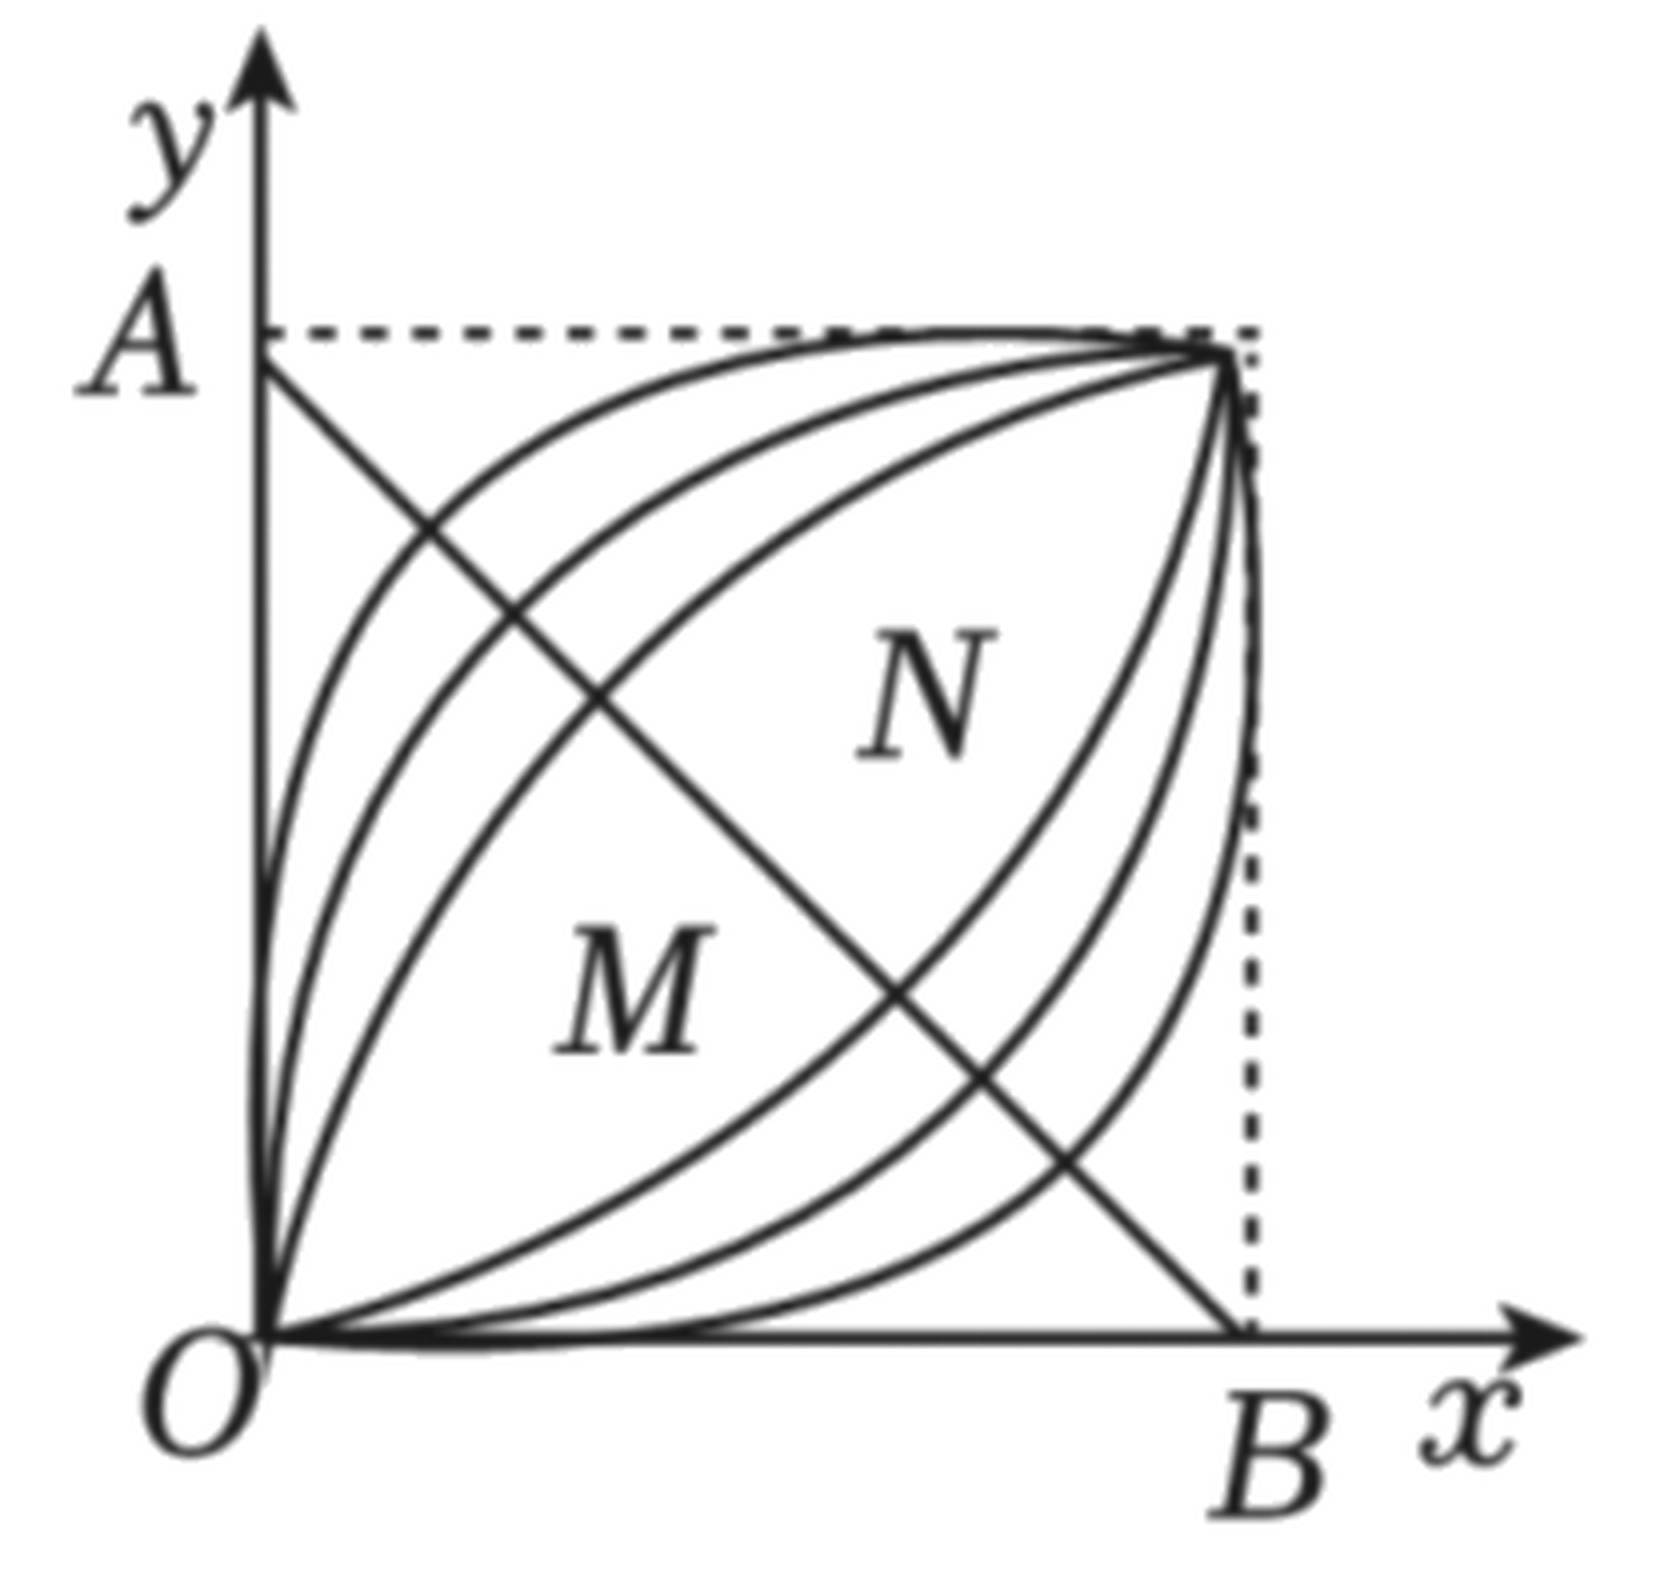
\includegraphics[width=0.40\textwidth]{figures/gao148_q12.png}
\end{center}

\ifanswer
\solbegin
\step{$BM=MN=NA$，点 $A(1,0)$，$B(0,1)$，所以 $M\left(\dfrac{1}{3},\dfrac{2}{3}\right)$，$N\left(\dfrac{2}{3},\dfrac{1}{3}\right)$，}
\step{分别代入 $y=x^\alpha$，$y=x^\beta$，$\alpha=\log_{\frac{2}{3}}\dfrac{1}{3},\beta=\log_{\frac{1}{3}}\dfrac{2}{3}$，$\alpha\beta=\log_{\frac{1}{3}}\dfrac{2}{3}\cdot\log_{\frac{2}{3}}\dfrac{1}{3}=1$.}
\solend
\fi

\end{enumerate}

\bigsec{二、选择题}

\begin{enumerate}
\setcounter{enumi}{12}

% === Q13 ===：答案"C"直接印在题干括号内、全卷无该题【答案】/【解析】段，按 高一84 Q13 成例括号留空、另提 \ans{$C$}；弯引号含空格
\item 若 $x$、$y\in\R$，则 “ $x=0$ ” 是 “ $xy=0$ ” 的\mbox{（\quad）}

\keepwithprev
A. 充要条件\qquad\qquad B. 必要不充分条件

C. 充分不必要条件\qquad\qquad D. 既不充分也不必要条件

\ifanswer
\ans{$C$}
\fi

% === Q14 ===：六个结论（圈数字在文本模式）、四选项一行；解析 8 行（对② 的两行公式各占一印刷行）
\item 若 $a<b<0$，下面有六个结论：① $a^2>b^2$；② $a^3<b^3$；③ $\dfrac{1}{a}<\dfrac{1}{b}$；④ $\dfrac{a}{b}>1$；⑤ $\dfrac{1}{a-b}>\dfrac{1}{a}$；⑥ $\lvert a\rvert>-b$. 其中正确的个数是\mbox{（\quad）}

\keepwithprev
A. 1\qquad\qquad B. 2\qquad\qquad C. 3\qquad\qquad D. 4

\ifanswer
\solbegin
\step{对①：$a^2-b^2=(a+b)(a-b),a+b<0,a-b<0$，故 $a^2-b^2>0$，正确；}
\step{对②：$a^3-b^3=(a-b)(a^2+ab+b^2)=(a-b)\left[\left(a+\dfrac{1}{2}b\right)^2+\dfrac{3}{4}b^2\right],a-b<0$，}
\step{$\left(a+\dfrac{1}{2}b\right)^2+\dfrac{3}{4}b^2>0$，故 $a^3-b^3<0$，正确；}
\step{对③：取 $a=-2,b=-1$，则 $\dfrac{1}{a}=-\dfrac{1}{2},\dfrac{1}{b}=-1,\dfrac{1}{a}>\dfrac{1}{b}$，错误；}
\step{对④：$\dfrac{a}{b}-1=\dfrac{a-b}{b},a-b<0,b<0$，故 $\dfrac{a}{b}-1>0$，正确；}
\step{对⑤：取 $a=-2,b=-1$，则 $\dfrac{1}{a-b}=-1,\dfrac{1}{a}=-\dfrac{1}{2},\dfrac{1}{a-b}<\dfrac{1}{a}$，错误；}
\step{对⑥：要证 $\lvert a\rvert>-b$，即 $-a>-b$，即 $a<b$，正确；}
\step{故选 $D$.}
\solend
\fi

% === Q15 ===：题目配图（四条指数函数曲线，三版都出），\needvspace 守卫放 \item 之前；"图象"照录；解析 5 行
\needvspace{8cm}
\item 如图，曲线①②③④分别是指数函数 $y=a^x$，$y=b^x$，$y=c^x$，$y=d^x$ 的图象，则实数 $a$、$b$、$c$、$d$ 的大小关系为\mbox{（\quad）}

\keepwithprev
A. $a<b<c<d$\qquad B. $b<a<d<c$\qquad C. $d<c<b<a$\qquad D. $c<d<a<b$

\begin{center}
% 四条指数函数曲线图取 04 页右侧，去粉色水印、去色、4× LANCZOS 放大；三版都出
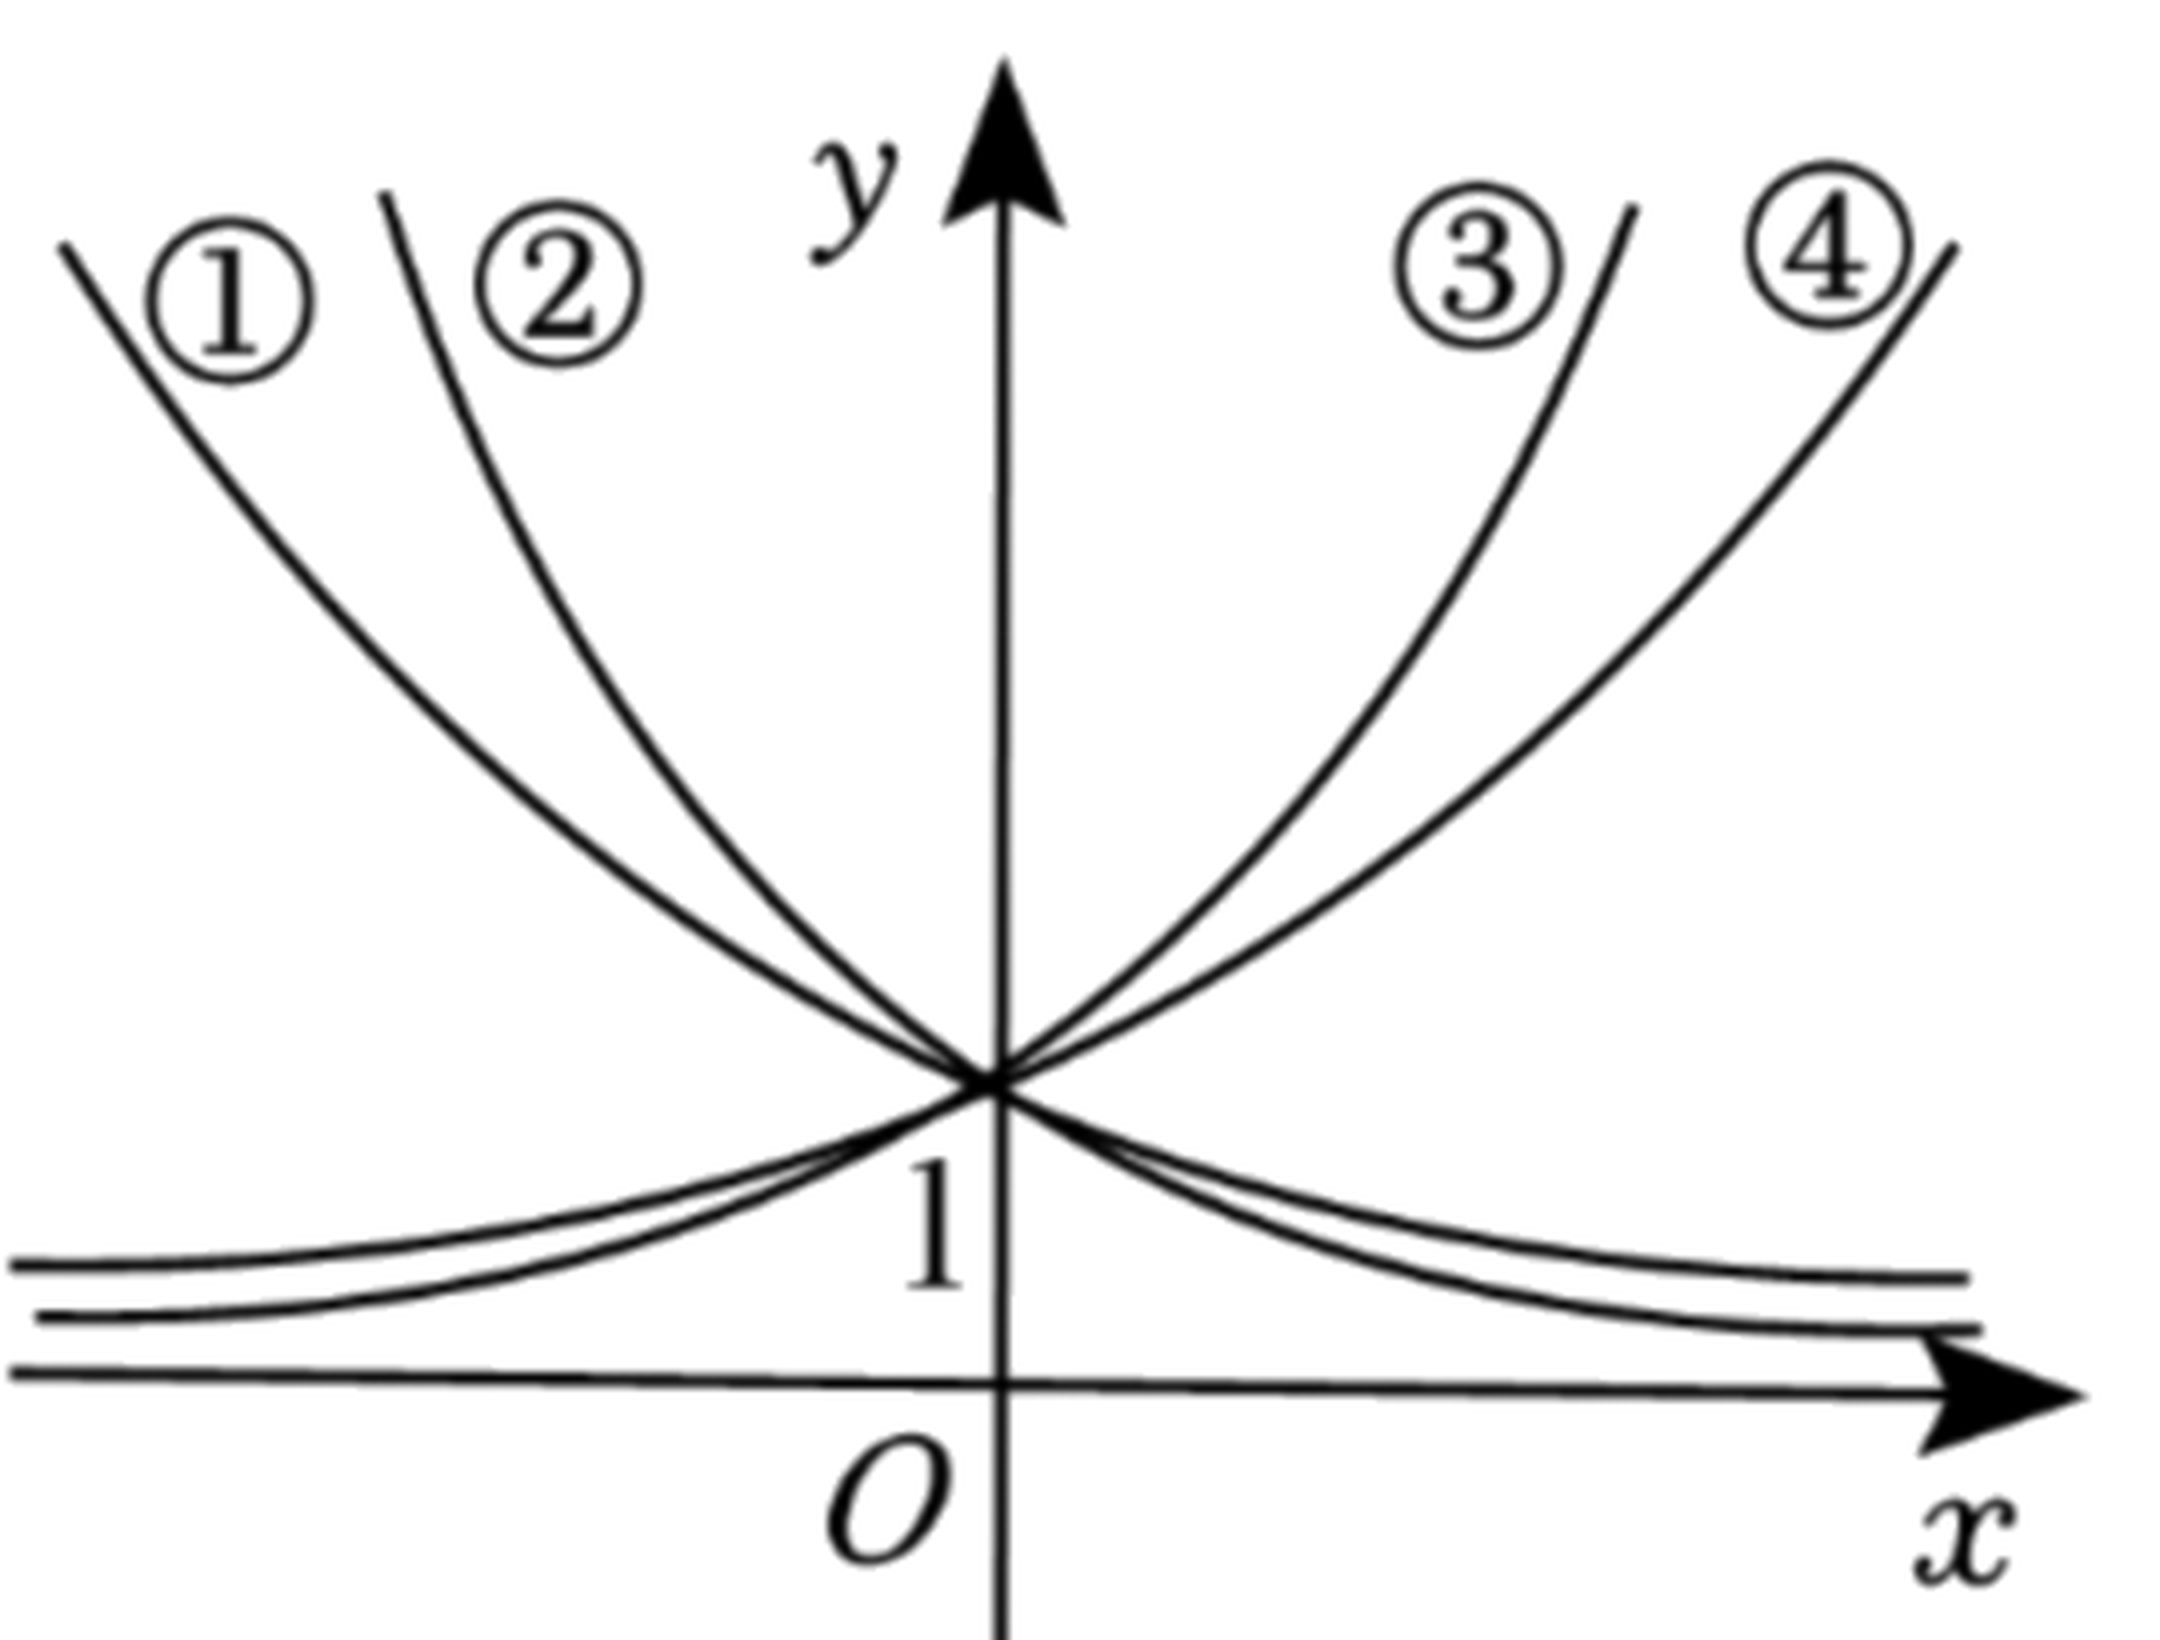
\includegraphics[width=0.40\textwidth]{figures/gao148_q15.png}
\end{center}

\ifanswer
\solbegin
\step{由函数图象得函数① $y=a^x$；② $y=b^x$ 为减函数，且 $x=1$ 时，$b^1<a^1$，}
\step{所以 $0<b<a<1$，}
\step{由函数图象得函数③ $y=c^x$；④ $y=d^x$ 为增函数，且 $x=1$ 时，$c^1>d^1$，}
\step{所以 $c>d>1$，}
\step{所以 $b<a<d<c$. 故选 $B$.}
\solend
\fi

% === Q16 ===：题目配图（关于 y 轴对称的幂函数曲线，三版都出），\needvspace 守卫放 \item 之前；$p$、$q\in\Z$；"图象"照录；解析 2 行
\needvspace{8cm}
\item 已知幂函数 $y=x^{\frac{p}{q}}$（$p$、$q\in\Z$ 且 $p$、$q$ 互质）的图象关于 $y$ 轴对称，如图所示，则\mbox{（\quad）}

\keepwithprev
A. $p$、$q$ 均为奇数，且 $\dfrac{p}{q}>0$\qquad\qquad B. $q$ 为偶数，$p$ 为奇数，且 $\dfrac{p}{q}<0$

C. $q$ 为奇数，$p$ 为偶数，且 $\dfrac{p}{q}>0$\qquad\qquad D. $q$ 为奇数，$p$ 为偶数，且 $\dfrac{p}{q}<0$

\begin{center}
% 关于 y 轴对称的幂函数曲线图取 04 页右下，去粉色水印、去色、4× LANCZOS 放大；三版都出
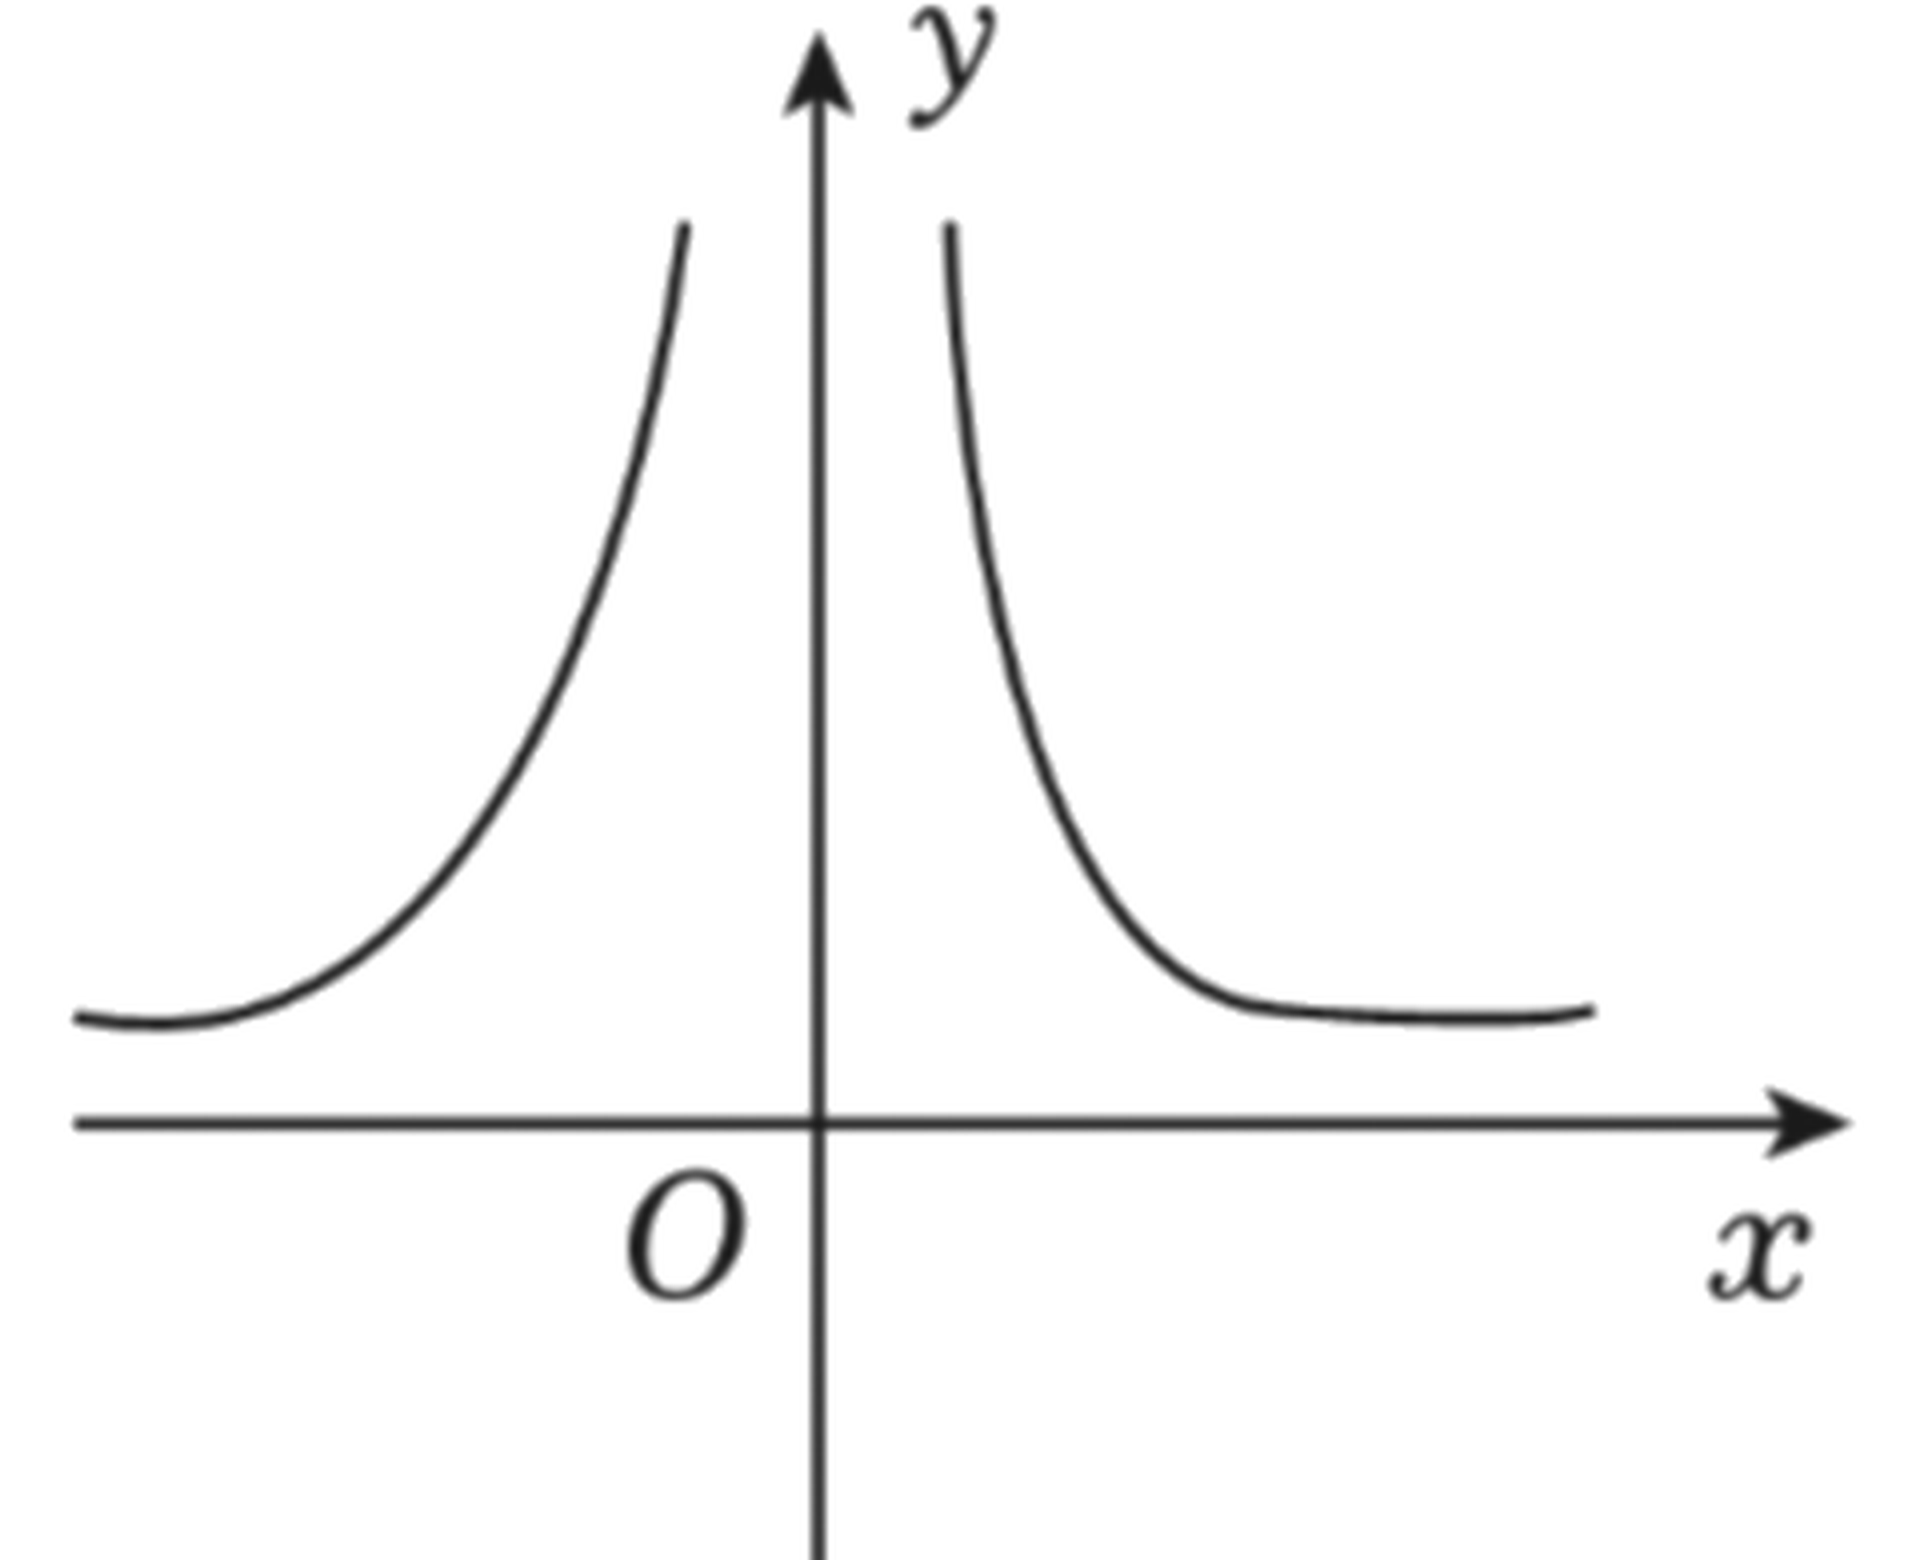
\includegraphics[width=0.36\textwidth]{figures/gao148_q16.png}
\end{center}

\ifanswer
\solbegin
\step{因为函数为偶函数，所以 $p$ 为偶数，且由图象形状判定 $\dfrac{p}{q}<0$.}
\step{又 $p$、$q$ 互质，所以 $q$ 为奇数. 故选 $D$.}
\solend
\fi

\end{enumerate}

\bigsec{三、解答题}

\begin{enumerate}
\setcounter{enumi}{16}

% === Q17 ===：\overline{B}／\varnothing／\R／\mid 逐处照录；解析 8 行
\item 已知集合 $A=\left\{x\mid \dfrac{5}{2x+1}>1\right\}$，$B=\{x\mid x^2+(a+3)x+3a<0,a\in\R\}$.

(1) 求 $A$.

(2) 若全集 $U=\R$，且 $A\cap\overline{B}=\varnothing$，求实数 $a$ 的取值范围.

\ifanswer
\solbegin
\step{(1) $\dfrac{5}{2x+1}>1$，即 $\dfrac{5}{2x+1}-1>0$，即 $\dfrac{4-2x}{2x+1}>0$，即 $(2x+1)(x-2)<0$，}
\step{解得 $-\dfrac{1}{2}<x<2$，所以 $A=\left(-\dfrac{1}{2},2\right)$；}
\step{(2) $x^2+(a+3)x+3a<0$，即 $(x+3)(x+a)<0$，}
\step{全集 $U=\R$，且 $A\cap\overline{B}=\varnothing$，}
\step{当 $a<3$ 时，解得 $-3<x<-a$，则 $\overline{B}=(-\infty,-3)\cup(-a,+\infty)$，}
\step{此时 $-a\geqslant2$，解得 $a\leqslant-2$，}
\step{当 $a\geqslant3$ 时，不满足 $A\cap\overline{B}=\varnothing$，}
\step{故实数 $a$ 的取值范围是 $(-\infty,-2]$.}
\solend
\fi

% === Q18 ===：cases 块整体算一个印刷行；解析 6 行
\item 已知幂函数经过点 $(2,4)$.

(1) 当 $x=\dfrac{1}{2}$ 时，求函数的值；

(2) 是否存在实数 $m$、$n$，使得该函数在区间 $[m,n]$ 上最小值为 $6m-8$，最大值为 $6n-8$？若存在，求出 $m$、$n$ 的值，若不存在，请说明理由.

\ifanswer
\solbegin
\step{(1) 设幂函数的解析式是 $y=x^\alpha$，则 $2^\alpha=4$，解得 $\alpha=2$，}
\step{故 $f(x)=x^2$，$f\left(\dfrac{1}{2}\right)=\dfrac{1}{4}$；}
\step{(2) 因为 $f(x)\geqslant0$，所以 $6m-8\geqslant0$，$m\geqslant\dfrac{4}{3}$，}
\step{由函数 $f(x)$ 在 $(0,+\infty)$ 严格增，得函数 $f(x)$ 在 $(m,n)$ 严格增，}
\step{所以 $\begin{cases}f(m)=6m-8\\f(n)=6n-8\end{cases}$ 且 $m<n$，解得 $m=2$，$n=4$，}
\step{故存在 $m=2$，$n=4$ 满足题意.}
\solend
\fi

% === Q19 ===：7 处评分档照 高一54／64 成例排 \dots\dots N 分；判别式高 \Delta；解析 9 行
\item 已知方程 $x^2+6mx+9m-2=0$，且 $x_1,x_2$ 是方程的两个不同的实数根.

(1) 若 $m=1$，求 $\dfrac{1}{x_1}+\dfrac{1}{x_2}$ 的值；

(2) 若 $m\in\R$，且 $x_1^2+x_2^2<4$，求 $m$ 取值范围.

\ifanswer
\solbegin
\step{(1) 当 $m=1$ 时，方程为 $x^2+6x+7=0$，\dots\dots1 分}
\step{则 $x_1+x_2=-6,x_1\cdot x_2=7$，\dots\dots2 分}
\step{$\dfrac{1}{x_1}+\dfrac{1}{x_2}=\dfrac{x_1+x_2}{x_1\cdot x_2}=-\dfrac{6}{7}$\dots\dots3 分}
\step{(2) $x_1+x_2=-6m,x_1\cdot x_2=9m-2$\dots\dots2 分}
\step{因为 $x_1^2+x_2^2=(x_1+x_2)^2-2x_1\cdot x_2$，所以 $(x_1+x_2)^2-2x_1\cdot x_2<4$，}
\step{所以 $36m^2-2(9m-2)<4$，解得 $0<m<\dfrac{1}{2}$\dots\dots2 分}
\step{又因为方程有两个不同的根，所以 $\Delta=36m^2-4(9m-2)>0$，}% 判别式原卷印等腰偏高粗三角 $\Delta$，照录（放大 07 页 q19_delta3.png／diag_band_q19.png 确认）
\step{解得 $m<\dfrac{1}{3}$ 或 $m>\dfrac{2}{3}$\dots\dots2 分}
\step{所以 $0<m<\dfrac{1}{3}$\dots\dots2 分}
\solend
\fi

% === Q20 ===：题目配图（矩形蔬菜温室，三版都出），\needvspace 守卫放 \item 之前；单位 \mathrm{m}／\mathrm{m}^2；解析 10 行
\needvspace{8cm}
\item 某村计划建造一个室内面积为 $600\mathrm{m}^2$ 的矩形蔬菜温室，在室内，沿左、右两侧与后侧内墙各保留 $2\mathrm{m}$ 宽的通道，沿前侧内墙保留 $4\mathrm{m}$ 宽的空地.

\begin{center}
% 矩形蔬菜温室示意图取 07 页右侧，去粉色水印、去色、4× LANCZOS 放大；三版都出
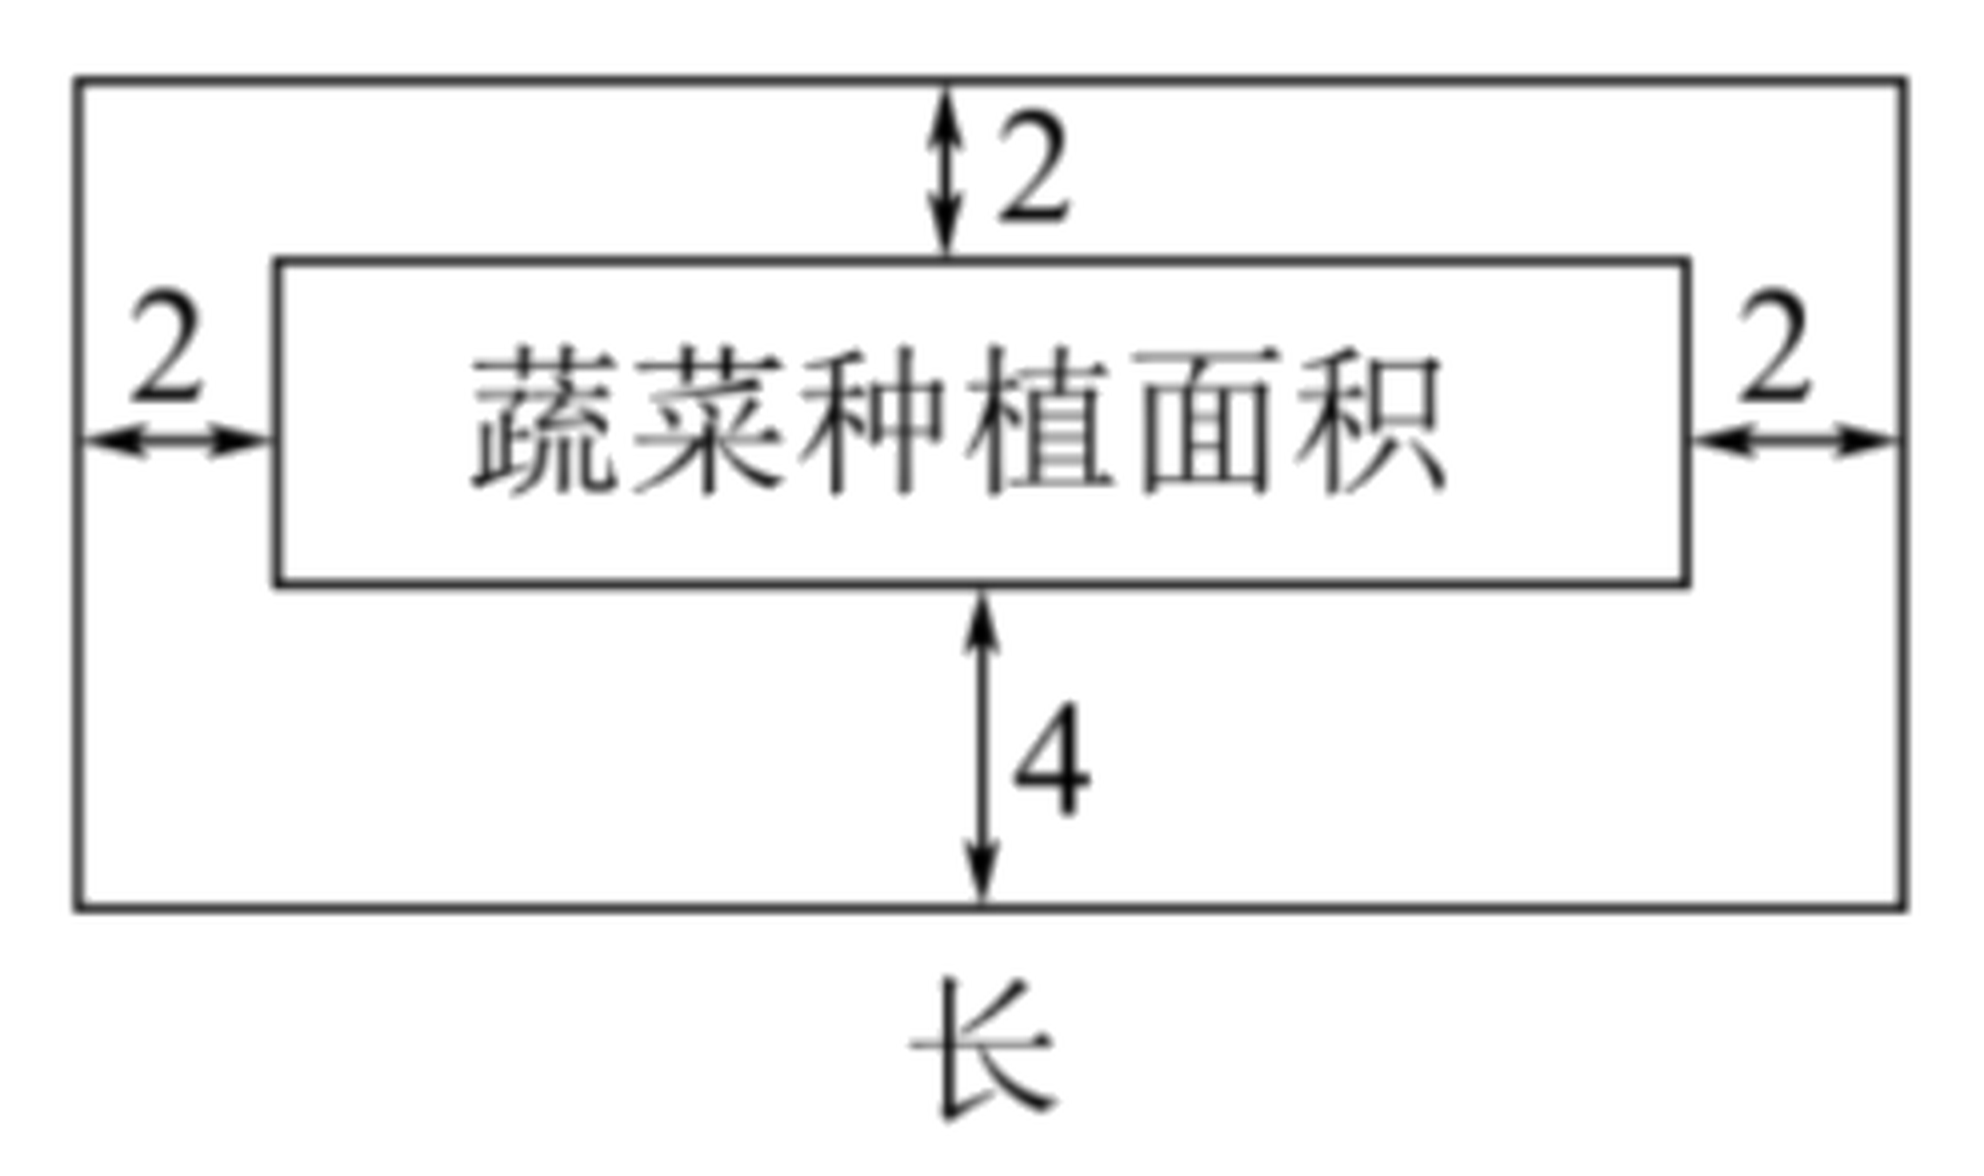
\includegraphics[width=0.45\textwidth]{figures/gao148_q20.png}
\end{center}

(1) 写出蔬菜的种植面积关于矩形温室的长之间的关系式.

(2) 当矩形温室的边长各为多少时，蔬菜的种植面积最大？最大种植面积是多少？

\ifanswer
\solbegin
\step{(1) 设蔬菜的种植面积为 $y\mathrm{m}^2$，矩形温室的长为 $x\mathrm{m}$，}
\step{则矩形温室的宽为 $\dfrac{600}{x}\mathrm{m}$，}
\step{种植蔬菜矩形的长为 $(x-4)\mathrm{m}$，宽为 $\left(\dfrac{600}{x}-6\right)\mathrm{m}$，}
\step{所以 $y=(x-4)\left(\dfrac{600}{x}-6\right)(4<x<100)$；}
\step{(2) 因为 $y=(x-4)\left(\dfrac{600}{x}-6\right)=624-\left(6x+\dfrac{2400}{x}\right)$，}
\step{因为 $6x+\dfrac{2400}{x}\geqslant2\sqrt{6x\cdot\dfrac{2400}{x}}=240$，}
\step{当且仅当 $6x=\dfrac{2400}{x}$，即 $x=20$ 时取等号，}
\step{所以 $y=624-\left(6x+\dfrac{2400}{x}\right)\leqslant624-240=384$.}
\step{即当矩形温室的一边长为 $20\mathrm{m}$，另一边长为 $30\mathrm{m}$ 时，}
\step{蔬菜的种植面积最大，最大为 $384\mathrm{m}^2$.}
\solend
\fi

% === Q21 ===：3 问、cases 块整体算一个印刷行；判别式高 \Delta；解析 19 行（末行续 09 页）
\item 二次函数 $f(x)=ax^2+bx+c$ 满足对任意的 $x\in\R$，$x-1\leqslant f(x)\leqslant x^2-x$ 恒成立.

(1) 求证：$f(1)$ 为定值；

(2) 若 $f(0)=-\dfrac{1}{4}$，求二次函数 $f(x)$ 的表达式；

(3) 求 $a+2b+5c$ 的取值范围.

\ifanswer
\solbegin
\step{(1) 对任意的 $x\in\R$，$x-1\leqslant f(x)\leqslant x^2-x$ 恒成立，则 $0\leqslant f(1)\leqslant0$，}
\step{所以 $f(1)=0$，为定值.}
\step{(2) 由(1)得 $a+b+c=f(1)=0$，由 $f(0)=-\dfrac{1}{4}$，得 $c=-\dfrac{1}{4}$，}
\step{则 $b=\dfrac{1}{4}-a$，$f(x)=ax^2+\left(\dfrac{1}{4}-a\right)x-\dfrac{1}{4}$，}
\step{不等式 $x-1\leqslant f(x)$ 可化为 $ax^2+\left(\dfrac{1}{4}-a\right)x-\dfrac{1}{4}\geqslant x-1$，}
\step{即 $ax^2-\left(a+\dfrac{3}{4}\right)x+\dfrac{3}{4}\geqslant0$，}
\step{一元二次不等式 $ax^2-\left(\dfrac{3}{4}+a\right)x+\dfrac{3}{4}\geqslant0$ 恒成立，则 $\begin{cases}a>0\\\Delta=\left(a+\dfrac{3}{4}\right)^2-3a\leqslant0\end{cases}$，}% 判别式原卷印等腰偏高粗三角 $\Delta$，照录（放大 08 页 q21_delta3.png／diag_band_q21.png 确认）
\step{解得 $a=\dfrac{3}{4}$，}
\step{此时 $f(x)=\dfrac{3}{4}x^2-\dfrac{1}{2}x-\dfrac{1}{4}$，$x^2-x-f(x)=\dfrac{1}{4}(x-1)^2\geqslant0$ 恒成立，}
\step{所以 $f(x)=\dfrac{3}{4}x^2-\dfrac{1}{2}x-\dfrac{1}{4}$.}
\step{(3) 由(1)得 $b=-a-c$，$f(x)=ax^2-(a+c)x+c=(ax-c)(x-1)$，}
\step{不等式 $x-1\leqslant f(x)$ 可化为 $(x-1)(ax-c-1)\geqslant0$，}
\step{一元二次不等式 $(x-1)(ax-c-1)\geqslant0$ 恒成立，则 $a>0$，}
\step{且方程 $(x-1)(ax-c-1)=0$ 有相等的实数根，因此 $c=a-1$，$a>0$，}
\step{不等式 $f(x)\leqslant x^2-x\Leftrightarrow(ax-c)(x-1)\leqslant x^2-x\Leftrightarrow(x-1)[(1-a)x+c]\geqslant0$，}
\step{同理 $1-a>0$，且方程 $(x-1)[(1-a)x+c]=0$ 有相等的实数根，}
\step{因此 $c=a-1$，$a<1$，从而 $c=a-1$，$b=1-2a$，$0<a<1$，}
\step{$a+2b+5c=a+2(1-2a)+5(a-1)=2a-3\in(-3,-1)$，}
\step{所以 $a+2b+5c$ 的取值范围是 $(-3,-1)$.}
\solend
\fi

\end{enumerate}

\end{document}
"
%
% ① 原始材料：微信公众号"魔都数学加油站"文章，连载"27学年高一148"，原文标题
% "27学年高一148——2026-2027年上海市新川中学高一上期中"（2026-11-21 推送）；
% 原文链接：https://mp.weixin.qq.com/s/Alhmwb3sSLQMp_wjzoAVyA 。
% 正文为 9 张 PNG 页（01/03/04/07/08/09 为 2560×3620，02/05/06 为 4762×6735，
% 同一篇各页分辨率混排，逐页按各自分辨率裁图核对，别按预览比例换算裁框）。
% 体例：混合体例讲评版——19 题中 Q4、Q5 只印【答案】、无【解析】；Q13 的答案"C"
% 直接印在题干括号内、无【答案】/【解析】段；其余 16 题印【解析】（逐题核实，见 ② ②）。
% 题目、答案、解析均据原图转录；卷面粉红色水印"魔都数学加油站"及公众号页脚未录入。
% 全卷插图清单（逐页通读 9 页确认）：4 幅题目配图，均三版都出、均非【解析】内配图：
%   · Q12 幂函数曲线族图（03 页右侧：x/y 轴、O、A(1,0)、B(0,1)、M、N 与两族
%     y=x^α／y=x^β 曲线、线段 AB、虚线），题干"（如图）"处，裁 figures/gao148_q12.png；
%   · Q15 四条指数函数曲线图（04 页右侧：①②③④ 四曲线同过 (0,1)、x/y 轴、O、
%     y 轴刻度 1），题干"如图"处，裁 figures/gao148_q15.png；
%   · Q16 关于 y 轴对称的幂函数曲线图（04 页右下：x/y 轴、O、两支上翘曲线），
%     题干"如图所示"处，裁 figures/gao148_q16.png；
%   · Q20 矩形蔬菜温室示意图（07 页右侧：大矩形＋内框"蔬菜种植面积"＋2/2/4
%     通道标注＋"长"），题干处，裁 figures/gao148_q20.png；
%   其余各页逐页确认无其它题目配图、无【解析】内配图、无表格，亦无"题干写如图而
%   源码漏图"一处；Q19 解析行末的虚线"----N 分"为评分档（非图），Q18／Q21 的
%   cases 块为数学块（非图）。4 图均取自原卷截图，去粉色水印、去色、4× LANCZOS 放大。
%
% 卷首标题：原卷印作"2026-2027 年新川中学高一上期中"，年份区间按全稿惯例排 en dash；
% 原卷卷面未印副标题，本稿按同期中卷（高一140／141／143／144／145／146／147）知识模块
% 口径补出"集合与常用逻辑用语、不等式、函数"。
%
% 题号体例（逐页核实定稿）：本卷共 19 题——一、填空题 3—12（10 题）、
% 二、选择题 13—16（4 题）、三、解答题 17—21（5 题）。
% 三节分别 \setcounter{enumi}{2}／{12}／{16}。原卷从第 3 题起、无第 1、2 题，
% 本稿保留原题号；全卷无附加题节、无 Q22（Q21 解析末行"所以 a+2b+5c 的取值范围是
% (-3,-1)."为全卷收尾，09 页下半仅水印、无正文）。
%
% ② 与原卷的排版差异：
%   ① 原文从第 3 题起，本稿保留原题号；共 19 题三节；
%   ② 混合体例逐题核实：Q4（反证法"假设的内容"）、Q5 只印【答案】、无【解析】，
%      按 高一140 第 5 题／高一145 Q3 成例提 \ans{}、不补造解析；Q13 答案"C"直接
%      印在题干括号内（" ( C ) "）、全卷无该题【答案】/【解析】段，按 高一84 Q13／
%      高一37 Q13／高一53 Q13 成例括号 \mbox{（\quad）} 留空、另提 \ans{$C$}；
%      其余 16 题印【解析】、用 \solbegin…\solend，选择题答案在解析末句"故选 X"
%      （Q14 选 D、Q15 选 B、Q16 选 D，逐个放大原图核实）、题干括号留空、不另提
%      \ans{}；答案版【答案】/【解析】标记数 = 19（3 个 \ans ＋ 16 个 \solbegin）
%      = 全卷题数；
%   ③ 原卷卷面未印副标题，本稿按知识模块口径补出；
%   ④ 原卷填空横线按全稿惯例排 \blankline[4.4em]；选择题括号排 \mbox{（\quad）}、
%      选项段前按惯例加 \keepwithprev；Q13／Q16 四选项为两行两列、Q14／Q15 选项
%      为一行，照原卷分行；解答题不留作答区、不加 \anspace（原卷为讲评版，
%      与 129／131／132／133／136／140／141／143／144／145／146 同）；
%   ⑤ 数集：Q11"在 R 上定义运算"、Q13"x、y∈R"、Q16"p、q∈Z"、Q17"a∈R"
%      "U=R"、Q19"m∈R"、Q21"x∈R" 原卷印斜体 R/Z，按全稿惯例统一改 \R／\Z
%      （本卷未出现 N，\N^* 无对应处）；绝对值排 \lvert…\rvert（Q9／Q14），
%      集合描述竖线排 \mid（Q17）；不等号按全稿惯例排 \leqslant／\geqslant；
%      补集照原卷上划线排 \overline{B}（Q17 题干 1 处＋解析 3 处）；空集
%      \varnothing（Q17 题干 1 处＋解析 2 处）；\subset（Q3 题干 {a}⊂M）与
%      \subseteq（Q3 题干 M⊆{a,b,c,d}）逐处照录不统一（放大 01 页 q3_subset.png）；
%   ⑥ 子题标号 (1)(2)(3) 半角括号照录；圈数字 ①—⑥ 在文本模式（Q14 六个结论、
%      Q15 曲线编号与其解析、Q14 解析"对①…对⑥"），按 common.sty 划入 CJK 字符类
%      渲染；cases 块整体算一个印刷行；\left…\right 不得拆到不同 $…$ 组；
%      单位 m／m² 排 \mathrm{m}／\mathrm{m}^2（Q20，原卷印正体 m）；
%   ⑦ 题干／解析中的中文弯引号按原卷照录：Q4" ab 可以被 5 整除，那么 a、b 中
%      至少有一个能被 5 整除 "（开引号后有空格、闭引号后空格接"时"）、
%      Q13" x=0 "" xy=0 "（引号内空格），注释内一律 ASCII 引号；
%   ⑧ 半角逗号在数学组之间是全稿惯例、非笔误（Q3"{a,b,c,d}"、Q6"$x,y$"
%      "$x=\frac13,y=\frac16$"、Q10、Q11"$a=-2,b=-1"、Q12"$\alpha=\log..,\beta=..$"、
%      Q14"$a+b<0,a-b<0$"、Q17、Q19"$x_1+x_2=-6,x_1\cdot x_2=7$"、Q20、Q21 等），
%      逐处照录别改全角；行末西文句点照录为 ASCII `.`；行中全角逗号／顿号照录；
%   ⑨ "图像／图象"逐处放大核：全卷 9 处均印"图象"（象，无亻）、未见"图像"，
%      逐处照录未统一改动（Q8 题干/解析各 1、Q12 题干 2、Q15 题干 1／解析 2、
%      Q16 题干 1／解析 1；放大 02/03/04/05 页 /tmp/gao148/zoom/my_wide_a.png、
%      my_wide_b.png 与宋体参考"象／像"并排确认）；
%   ⑩ 判别式 Δ/△ 混用是照录项：Q11 解析"△=1−4(−a²+a+1)<0"印扁等边空心
%      三角 \triangle；Q19 解析"Δ=36m²−4(9m−2)>0"、Q21 解析 cases 块
%      "Δ=(a+3/4)²−3a≤0" 两处印等腰偏高粗三角 \Delta，逐处放大判断、照录
%      不统一（参照 高一142／144／145 头注④口径，详见 ④）；
%   ⑪ 一条 \step = 原卷解析的一个印刷行，cases 块整体算一个印刷行；别把原卷折行
%      并起来、别把一行拆多条。Q3 六行、Q7 五行（01 页末首行＋02 页顶四行）、
%      Q9 七行、Q11 五行、Q14 八行（对② 的两行公式各占一印刷行）、Q17 八行、
%      Q18 六行、Q19 九行（7 处评分档附在行末）、Q20 十行、Q21 十九行
%      均按印刷行逐条断，不丢行；
%   ⑫ 配图：4 幅均为题目配图（三版都出），放 \item 内题干之后 \begin{center}；
%      大图块加 \needvspace 守卫把整块推走（守卫放 \item 之前，见 高一145 Q14/Q20
%      成例与切页审计 B 类坑）；三版切页审计均"合计异常：无"；
%   ⑬ 跨页续印按题合并：Q3/4/5 在 01 页；Q6 题干＋解析在 01 页；Q7 题干在 01 页
%      末、解析首行在 01 页末续 02 页顶四行；Q8/9/10 在 02 页（Q9 解析续 02 页下半、
%      Q10 题干与解析前 2 行在 02 页末）；Q10 解析末行续 03 页顶；Q11/12 在 03 页、
%      "二、选择题"标题与 Q13/14 题干在 03 页下半；Q13 无解析；Q14 解析在 04 页顶、
%      Q15 题干＋图＋选项＋解析在 04 页、Q16 题干＋图在 04 页末；Q16 选项＋解析＋
%      "三、解答题"标题＋Q17 题干＋解析在 05 页、Q18 题干首句在 05 页末；Q18 题干
%      续＋解析、Q19 题干＋解析前 5 行在 06 页；Q19 解析续 4 行＋Q20 题干＋图＋
%      解析（10 行全部）在 07 页，末行"蔬菜的种植面积最大，最大为 384m²."收尾；
%      Q21 题干＋解析前 18 行在 08 页；Q21 解析末行"所以 a+2b+5c 的取值范围是
%      (-3,-1)."在 09 页上半（09 页下半仅水印、无正文）。本稿按题连排，不丢行、
%      不并折行；
%   ⑭ 原卷解析内无红色"法一／法二"之类小标题，故本卷无 \stepm；水印
%      "魔都数学加油站"红色不录入；Q19 解析 7 处评分档（1/2/3/2/2/2/2 分）
%      原卷在行末印一串虚线，本稿照 高一54／64 成例排 \dots\dots N 分，
%      分值逐处照录、位置不变。
%
% ③ 行数复核：一条 \step／\stepm = 原卷解析的一个印刷行，cases 块作一个印刷行计。
%   逐题数（主会话逐页核对定稿）：Q3：6；Q4：0（只印【答案】、提 \ans{}）；
%   Q5：0（只印【答案】、提 \ans{}）；Q6：2；Q7：5；Q8：2；Q9：7；Q10：3；
%   Q11：5；Q12：2；Q13：0（答案印在题干括号内、另提 \ans{}）；Q14：8；Q15：5；
%   Q16：2；Q17：8；Q18：6；Q19：9；Q20：10；Q21：19。
%   合计 99 条 \step（本卷无 \stepm：解析内无红色"法一／法二"类小标题），
%   与原卷逐题印刷行相等。全卷 16 题设 \solbegin…\solend ＋ 3 处 \ans{}，
%   答案版【答案】/【解析】标记数 = 19 = 全卷题数。
%
% ④ 判别式／子集符号结论（逐处放大原图照录、不得统一，主会话像素级复核）：
%   判别式全卷 3 处，两形混用逐处照录不统一（参照 高一142／144／145 头注④口径）：
%     · Q11 解析"△=1−4(−a²+a+1)<0" 原卷印扁等边空心三角（宽>高、细线），
%       照录 \triangle（放大 03 页 /tmp/gao148/zoom/q11_delta3.png、
%       delta_montage.png 确认）；
%     · Q19 解析"Δ=36m²−4(9m−2)>0" 原卷印等腰偏高粗三角（高>宽），
%       照录 \Delta（放大 07 页 /tmp/gao148/zoom/q19_delta3.png 确认）；
%     · Q21 解析 cases 块"Δ=(a+3/4)²−3a≤0" 原卷印等腰偏高粗三角（高>宽），
%       照录 \Delta（放大 08 页 /tmp/gao148/zoom/q21_delta3.png 确认）。
%   子集／补集：Q3 题干"{a}⊂M⊆{a,b,c,d}" 前者印单线 ⊂、无下划线，照录 \subset；
%     后者印带下划线 ⊆，照录 \subseteq（放大 01 页 /tmp/gao148/zoom/q3_subset.png
%     确认）；Q17 题干 1 处＋解析 3 处共 4 处 \overline{B} 照原卷上划线
%     （B 上横线、非 C_U B）；空集 \varnothing 3 处（Q17 题干 1 处、解析 2 处）；
%     Q17 集合描述竖线 \mid；数集 \R／\Z 归一见 ② ⑤。
%
% ⑤ 存疑照录（放大原图确认，照录未改、正文对应处另有 % 注）：
%   1. Q3 解析末行"所以 M 一共有 3+3+1+1=8 个" 原卷印 $3+3+1+1=8$，按上文
%      四行应为 $1+3+3+1=8$（疑为原卷加数顺序笔误，和仍为 8），放大 01 页
%      /tmp/gao148/zoom/my_q3_sol.png 确认，照录未改。
%   2. Q13 答案"C"直接印在题干括号内、全卷无该题【答案】/【解析】段，按
%      高一84 Q13 成例括号留空、另提 \ans{$C$}（见 ② ②），未补造解析。
%   3. Q19 解析 7 处评分档（"----N 分"）原卷印一串虚线，本稿照 高一54／64
%      成例排 \dots\dots N 分，分值逐处照录、位置不变。
%   4. 判别式 Q11 扁 \triangle 与 Q19／Q21 高 \Delta 两形混用，逐处照录不统一（见 ④）。
%   5. "图像／图象"全卷 9 处均印"图象"、未见"图像"（见 ② ⑨），逐处放大核实照录，
%      未统一改动。
%   全卷除此 5 类外未发现其它笔误／自相矛盾处。
%
% ⑥ 跨页续印按题合并说明：见 ② ⑬。
%
\documentclass[a4paper,11pt]{article}
\usepackage{common}

\begin{document}

\examtitlest[3]{2026--2027 年新川中学高一上期中}{集合与常用逻辑用语、不等式、函数}

\bigsec{一、填空题}

\begin{enumerate}
\setcounter{enumi}{2}

% === Q3 ===：题干 {a}⊂M⊆{a,b,c,d} 两个子集符号逐处照录；解析 6 行
\item 满足 $\{a\}\subset M\subseteq\{a,b,c,d\}$ 的集合 $M$ 有\blankline[4.4em]个.

\ifanswer
\solbegin
\step{$M$ 是 $\{a,b,c,d\}$ 的子集，但必含有元素 $a$，}
\step{当 $M$ 中只一个元素时，$M=\{a\}$ 只有 1 个；}
\step{当 $M$ 中有二个元素时，$M$ 有 3 个；}
\step{当 $M$ 中有三个元素时，$M$ 有 3 个；}
\step{当 $M$ 中有四个元素时，$M$ 有 1 个；}
\step{所以 $M$ 一共有 $3+3+1+1=8$ 个.}% 原卷印 $3+3+1+1=8$（按上文四行应为 $1+3+3+1$），疑为加数顺序笔误，照录未改（放大 01 页 my_q3_sol.png）
\solend
\fi

% === Q4 ===：原卷只印【答案】、无【解析】，按 高一140 第 5 题成例提 \ans{}；弯引号与空格照录
\item 用反证法证明命题 “ $ab$ 可以被 5 整除，那么 $a$、$b$ 中至少有一个能被 5 整除” 时假设的内容应该是\blankline[4.4em].

\ifanswer
\ans{$a$、$b$ 都不能被 5 整除}
\fi

% === Q5 ===：原卷只印【答案】 $[-2,1)$、无【解析】，提 \ans{}
\item 不等式 $\dfrac{x+2}{x-1}\leqslant0$ 的解集为\blankline[4.4em].

\ifanswer
\ans{$[-2,1)$}
\fi

% === Q6 ===：解析 2 行；半角逗号在数学组之间照录
\item 设 $x,y\in(0,+\infty)$，且 $x+4y=1$，则 $\dfrac{1}{x}+\dfrac{1}{y}$ 的最小值为\blankline[4.4em].

\ifanswer
\solbegin
\step{因为 $\dfrac{1}{x}+\dfrac{1}{y}=(x+4y)\left(\dfrac{1}{x}+\dfrac{1}{y}\right)=5+\dfrac{4y}{x}+\dfrac{x}{y}\geqslant5+2\sqrt{\dfrac{4y}{x}\cdot\dfrac{x}{y}}=9$，}
\step{当且仅当 $\dfrac{4y}{x}=\dfrac{x}{y}$，即 $x=2y$，即 $x=\dfrac{1}{3},y=\dfrac{1}{6}$ 时取等号，故最小值为 9.}
\solend
\fi

% === Q7 ===：题干在 01 页末、解析首行在 01 页末续 02 页顶四行；解析 5 行
\item 若不等式 $x^2+ax+b<0$ 的解集为 $(-3,-1)$，则不等式 $bx^2+ax+1\leqslant0$ 的解集为\blankline[4.4em].

\ifanswer
\solbegin
\step{不等式 $x^2+ax+b<0$ 的解集为 $(-3,-1)$，}
\step{所以方程 $x^2+ax+b=0$ 的两个实数根为 $-3$ 和 $-1$，}
\step{由根与系数的关系得 $a=4$，$b=3$，}
\step{故 $bx^2+ax+1\leqslant0$ 可化为 $3x^2+4x+1\leqslant0$，解得 $-1\leqslant x\leqslant-\dfrac{1}{3}$，}
\step{所求不等式 $bx^2+ax+1\leqslant0$ 的解集为 $\left[-1,-\dfrac{1}{3}\right]$.}
\solend
\fi

% === Q8 ===："图象"照录；解析 2 行
\item 函数 $y=a^{x-2}+2(a>0,a\ne1)$ 的图象必经过定点\blankline[4.4em].

\ifanswer
\solbegin
\step{令 $x-2=0$，得 $x=2$，则 $y=a^0+2=3$，}
\step{所以函数 $y=a^{x-2}+2$ 的图象过定点 $(2,3)$.}
\solend
\fi

% === Q9 ===：解析 7 行；首句末西文句点照录
\item 不等式 $\lvert x+3\rvert+\lvert a-x\rvert>6$ 对一切实数 $x$ 恒成立，则实数 $a$ 的取值范围为\blankline[4.4em].

\ifanswer
\solbegin
\step{$\lvert x+3\rvert$ 表示 $x$ 到 $-3$ 的距离，$\lvert a-x\rvert$ 表示 $x$ 到 $a$ 的距离.}
\step{所以它们的和为 $x$ 到 $-3$ 和 $x$ 到 $a$ 的距离之和，}
\step{当 $x$ 位于 $-3$ 和 $a$ 之间时，距离和取得最小值，}
\step{即两点之间的距离 $\lvert a-(-3)\rvert=\lvert a+3\rvert$，}
\step{若最小值 $\lvert a+3\rvert>6$，则原式对所有 $x$ 恒成立.}
\step{解得 $a+3>6$ 或 $a+3<-6$，即 $a>3$ 或 $a<-9$，}
\step{故 $a\in(3,+\infty)$ 或 $a\in(-\infty,-9)$.}
\solend
\fi

% === Q10 ===：题干与解析前 2 行在 02 页末、解析末行续 03 页顶；解析 3 行
\item 已知 $2^a=3$，$\log_3 5=b$，则 $\log_{15}20=$\blankline[4.4em]（用 $a$、$b$ 表示）.

\ifanswer
\solbegin
\step{因为 $2^a=3$，所以 $a=\log_2 3=\dfrac{\lg3}{\lg2}$，又 $\log_3 5=b=\dfrac{\lg5}{\lg3}$，}
\step{所以 $\lg3=a\lg2$，$\lg5=b\lg3=ba\lg2$，}
\step{则 $\log_{15}20=\dfrac{2\lg2+\lg5}{\lg3+\lg5}=\dfrac{2\lg2+ab\lg2}{a\lg2+ab\lg2}=\dfrac{2+ab}{a+ab}$.}
\solend
\fi

% === Q11 ===：在 \R 上定义运算 \otimes；判别式扁 \triangle 照录；解析 5 行
\item 在 $\R$ 上定义运算 $\otimes:x\otimes y=x(1-y)$，若不等式 $(x-a)\otimes(x+a)<1$ 对任意实数 $x$ 恒成立，则 $a$ 的取值范围是\blankline[4.4em].

\ifanswer
\solbegin
\step{由题意得不等式 $(x-a)\otimes(x+a)<1$ 对任意实数 $x$ 恒成立，}
\step{即不等式 $(x-a)(1-x-a)<1$ 对任意实数 $x$ 恒成立，}
\step{即 $x^2-x-a^2+a+1>0$ 对任意实数 $x$ 恒成立，}
\step{所以 $\triangle=1-4(-a^2+a+1)<0$，解得 $-\dfrac{1}{2}<a<\dfrac{3}{2}$，}% 判别式原卷印扁等边空心三角 $\triangle$，照录（放大 03 页 q11_delta3.png 确认）
\step{所以实数 $a$ 的取值范围为 $\left(-\dfrac{1}{2},\dfrac{3}{2}\right)$.}
\solend
\fi

% === Q12 ===：题目配图（幂函数曲线族，三版都出）；"图象"照录；解析 2 行
\needvspace{8cm}
\item 幂函数 $y=x^\alpha$，当 $\alpha$ 取不同的正数时，在区间 $[0,1]$ 上它们的图象是一族美丽的曲线（如图）. 设点 $A(1,0)$，$B(0,1)$，连接 $AB$，线段 $AB$ 恰好被其中的两个幂函数 $y=x^\alpha$，$y=x^\beta$ 的图象三等分，即有 $BM=MN=NA$，那么 $\alpha\beta=$\blankline[4.4em].

\begin{center}
% 幂函数曲线族图取 03 页右侧，去粉色水印、去色、4× LANCZOS 放大；三版都出
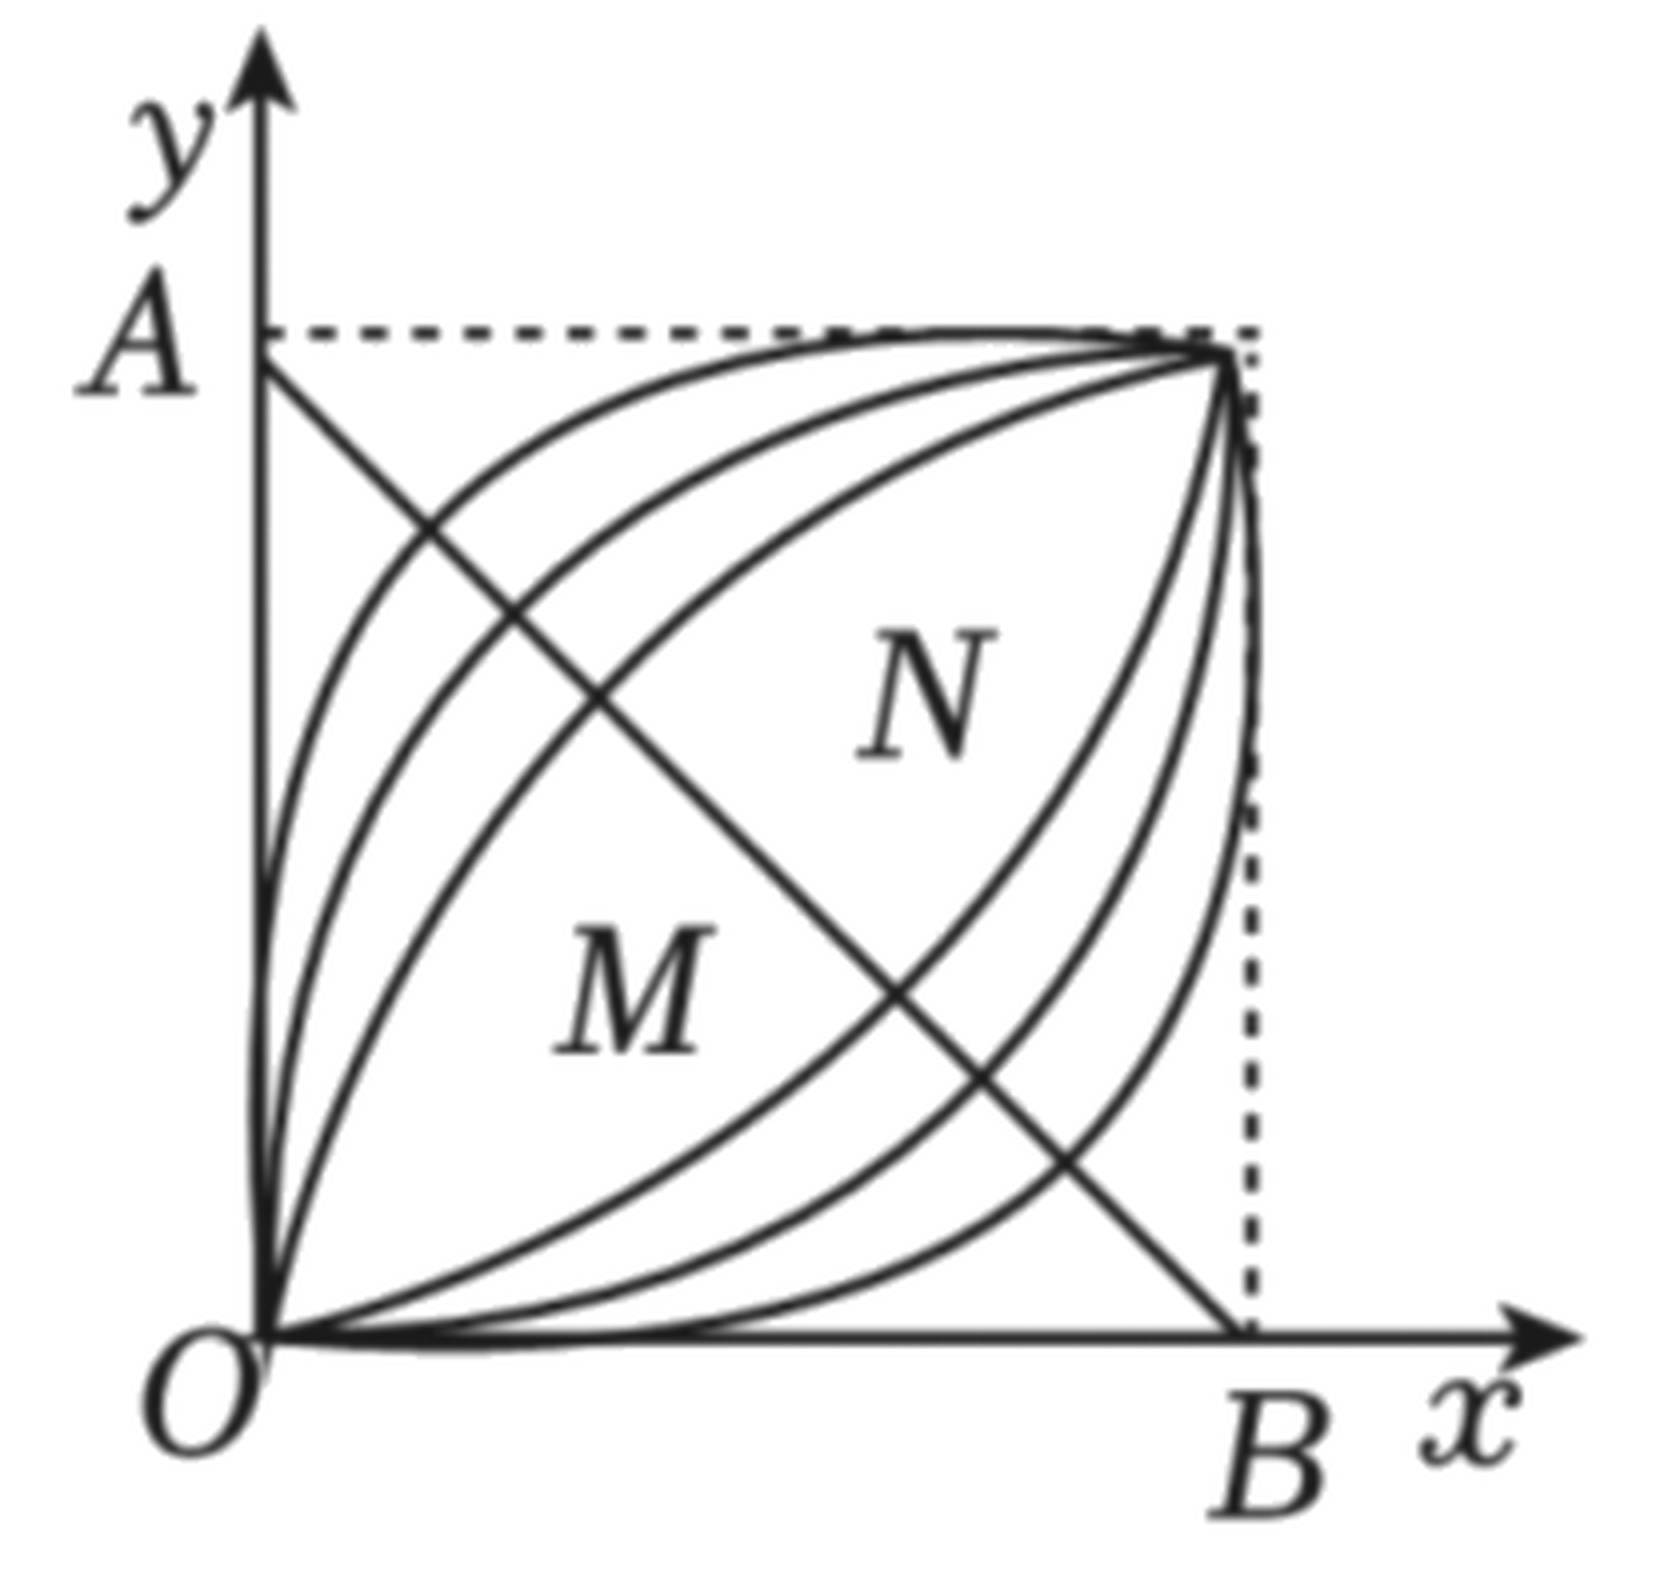
\includegraphics[width=0.40\textwidth]{figures/gao148_q12.png}
\end{center}

\ifanswer
\solbegin
\step{$BM=MN=NA$，点 $A(1,0)$，$B(0,1)$，所以 $M\left(\dfrac{1}{3},\dfrac{2}{3}\right)$，$N\left(\dfrac{2}{3},\dfrac{1}{3}\right)$，}
\step{分别代入 $y=x^\alpha$，$y=x^\beta$，$\alpha=\log_{\frac{2}{3}}\dfrac{1}{3},\beta=\log_{\frac{1}{3}}\dfrac{2}{3}$，$\alpha\beta=\log_{\frac{1}{3}}\dfrac{2}{3}\cdot\log_{\frac{2}{3}}\dfrac{1}{3}=1$.}
\solend
\fi

\end{enumerate}

\bigsec{二、选择题}

\begin{enumerate}
\setcounter{enumi}{12}

% === Q13 ===：答案"C"直接印在题干括号内、全卷无该题【答案】/【解析】段，按 高一84 Q13 成例括号留空、另提 \ans{$C$}；弯引号含空格
\item 若 $x$、$y\in\R$，则 “ $x=0$ ” 是 “ $xy=0$ ” 的\mbox{（\quad）}

\keepwithprev
A. 充要条件\qquad\qquad B. 必要不充分条件

C. 充分不必要条件\qquad\qquad D. 既不充分也不必要条件

\ifanswer
\ans{$C$}
\fi

% === Q14 ===：六个结论（圈数字在文本模式）、四选项一行；解析 8 行（对② 的两行公式各占一印刷行）
\item 若 $a<b<0$，下面有六个结论：① $a^2>b^2$；② $a^3<b^3$；③ $\dfrac{1}{a}<\dfrac{1}{b}$；④ $\dfrac{a}{b}>1$；⑤ $\dfrac{1}{a-b}>\dfrac{1}{a}$；⑥ $\lvert a\rvert>-b$. 其中正确的个数是\mbox{（\quad）}

\keepwithprev
A. 1\qquad\qquad B. 2\qquad\qquad C. 3\qquad\qquad D. 4

\ifanswer
\solbegin
\step{对①：$a^2-b^2=(a+b)(a-b),a+b<0,a-b<0$，故 $a^2-b^2>0$，正确；}
\step{对②：$a^3-b^3=(a-b)(a^2+ab+b^2)=(a-b)\left[\left(a+\dfrac{1}{2}b\right)^2+\dfrac{3}{4}b^2\right],a-b<0$，}
\step{$\left(a+\dfrac{1}{2}b\right)^2+\dfrac{3}{4}b^2>0$，故 $a^3-b^3<0$，正确；}
\step{对③：取 $a=-2,b=-1$，则 $\dfrac{1}{a}=-\dfrac{1}{2},\dfrac{1}{b}=-1,\dfrac{1}{a}>\dfrac{1}{b}$，错误；}
\step{对④：$\dfrac{a}{b}-1=\dfrac{a-b}{b},a-b<0,b<0$，故 $\dfrac{a}{b}-1>0$，正确；}
\step{对⑤：取 $a=-2,b=-1$，则 $\dfrac{1}{a-b}=-1,\dfrac{1}{a}=-\dfrac{1}{2},\dfrac{1}{a-b}<\dfrac{1}{a}$，错误；}
\step{对⑥：要证 $\lvert a\rvert>-b$，即 $-a>-b$，即 $a<b$，正确；}
\step{故选 $D$.}
\solend
\fi

% === Q15 ===：题目配图（四条指数函数曲线，三版都出），\needvspace 守卫放 \item 之前；"图象"照录；解析 5 行
\needvspace{8cm}
\item 如图，曲线①②③④分别是指数函数 $y=a^x$，$y=b^x$，$y=c^x$，$y=d^x$ 的图象，则实数 $a$、$b$、$c$、$d$ 的大小关系为\mbox{（\quad）}

\keepwithprev
A. $a<b<c<d$\qquad B. $b<a<d<c$\qquad C. $d<c<b<a$\qquad D. $c<d<a<b$

\begin{center}
% 四条指数函数曲线图取 04 页右侧，去粉色水印、去色、4× LANCZOS 放大；三版都出
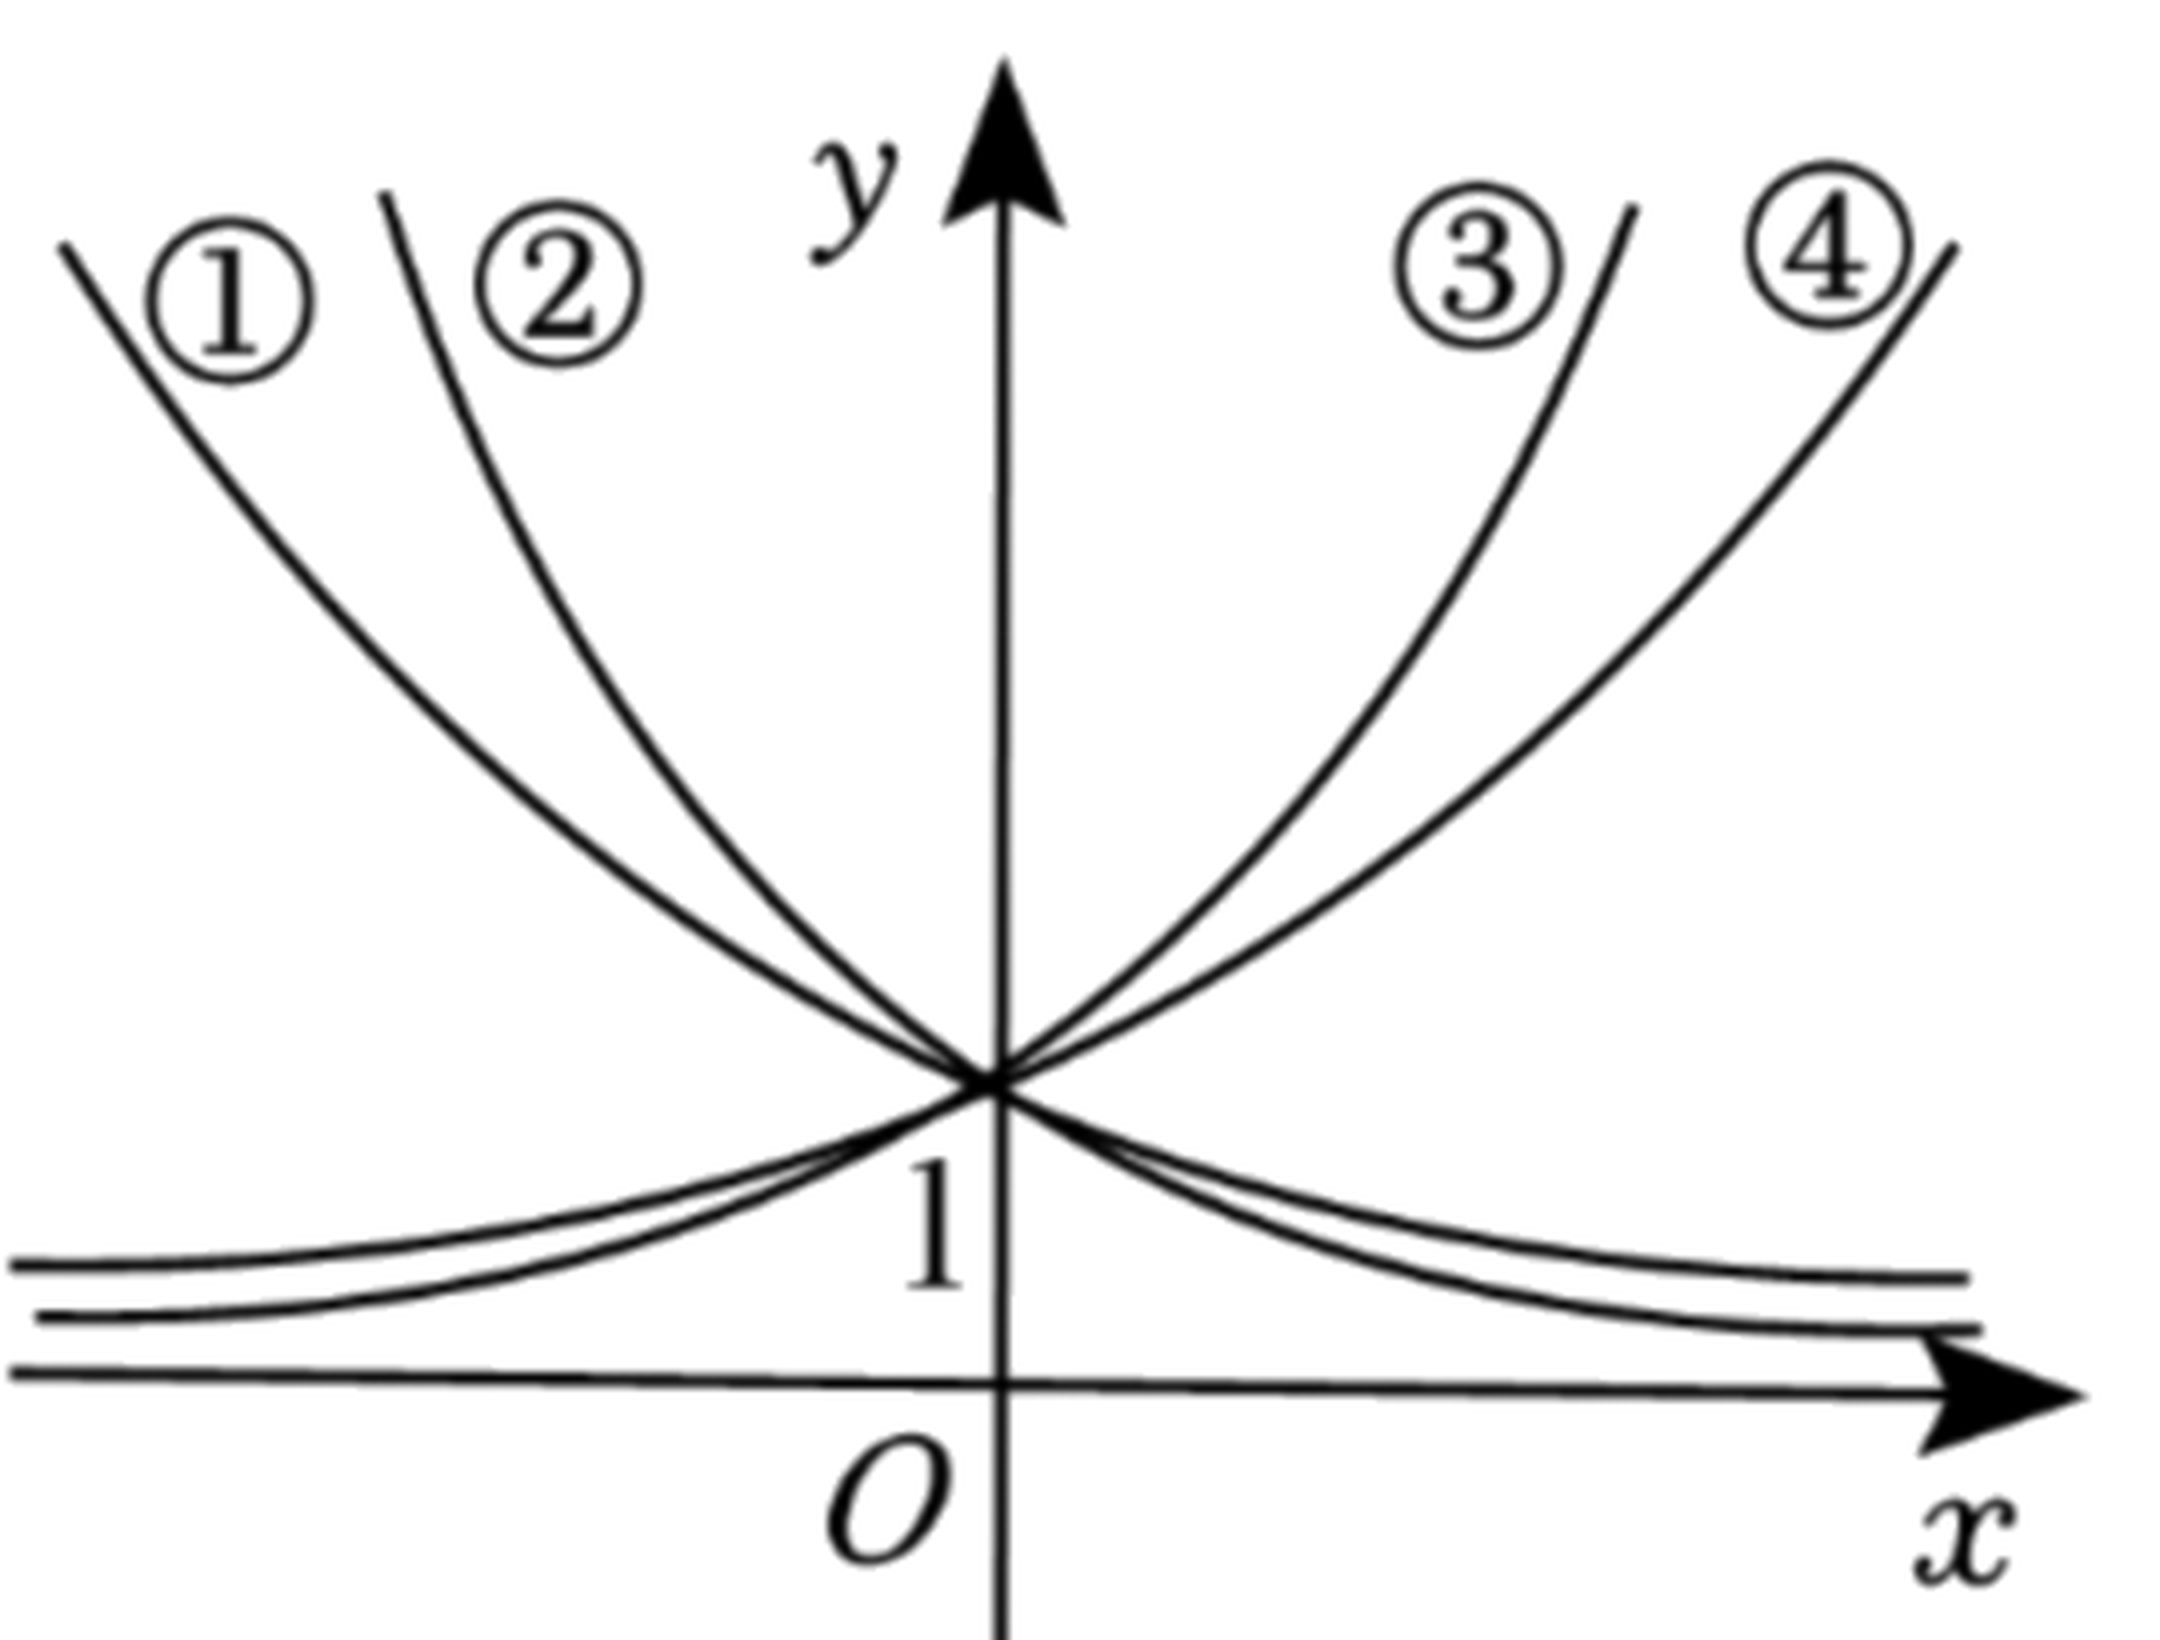
\includegraphics[width=0.40\textwidth]{figures/gao148_q15.png}
\end{center}

\ifanswer
\solbegin
\step{由函数图象得函数① $y=a^x$；② $y=b^x$ 为减函数，且 $x=1$ 时，$b^1<a^1$，}
\step{所以 $0<b<a<1$，}
\step{由函数图象得函数③ $y=c^x$；④ $y=d^x$ 为增函数，且 $x=1$ 时，$c^1>d^1$，}
\step{所以 $c>d>1$，}
\step{所以 $b<a<d<c$. 故选 $B$.}
\solend
\fi

% === Q16 ===：题目配图（关于 y 轴对称的幂函数曲线，三版都出），\needvspace 守卫放 \item 之前；$p$、$q\in\Z$；"图象"照录；解析 2 行
\needvspace{8cm}
\item 已知幂函数 $y=x^{\frac{p}{q}}$（$p$、$q\in\Z$ 且 $p$、$q$ 互质）的图象关于 $y$ 轴对称，如图所示，则\mbox{（\quad）}

\keepwithprev
A. $p$、$q$ 均为奇数，且 $\dfrac{p}{q}>0$\qquad\qquad B. $q$ 为偶数，$p$ 为奇数，且 $\dfrac{p}{q}<0$

C. $q$ 为奇数，$p$ 为偶数，且 $\dfrac{p}{q}>0$\qquad\qquad D. $q$ 为奇数，$p$ 为偶数，且 $\dfrac{p}{q}<0$

\begin{center}
% 关于 y 轴对称的幂函数曲线图取 04 页右下，去粉色水印、去色、4× LANCZOS 放大；三版都出
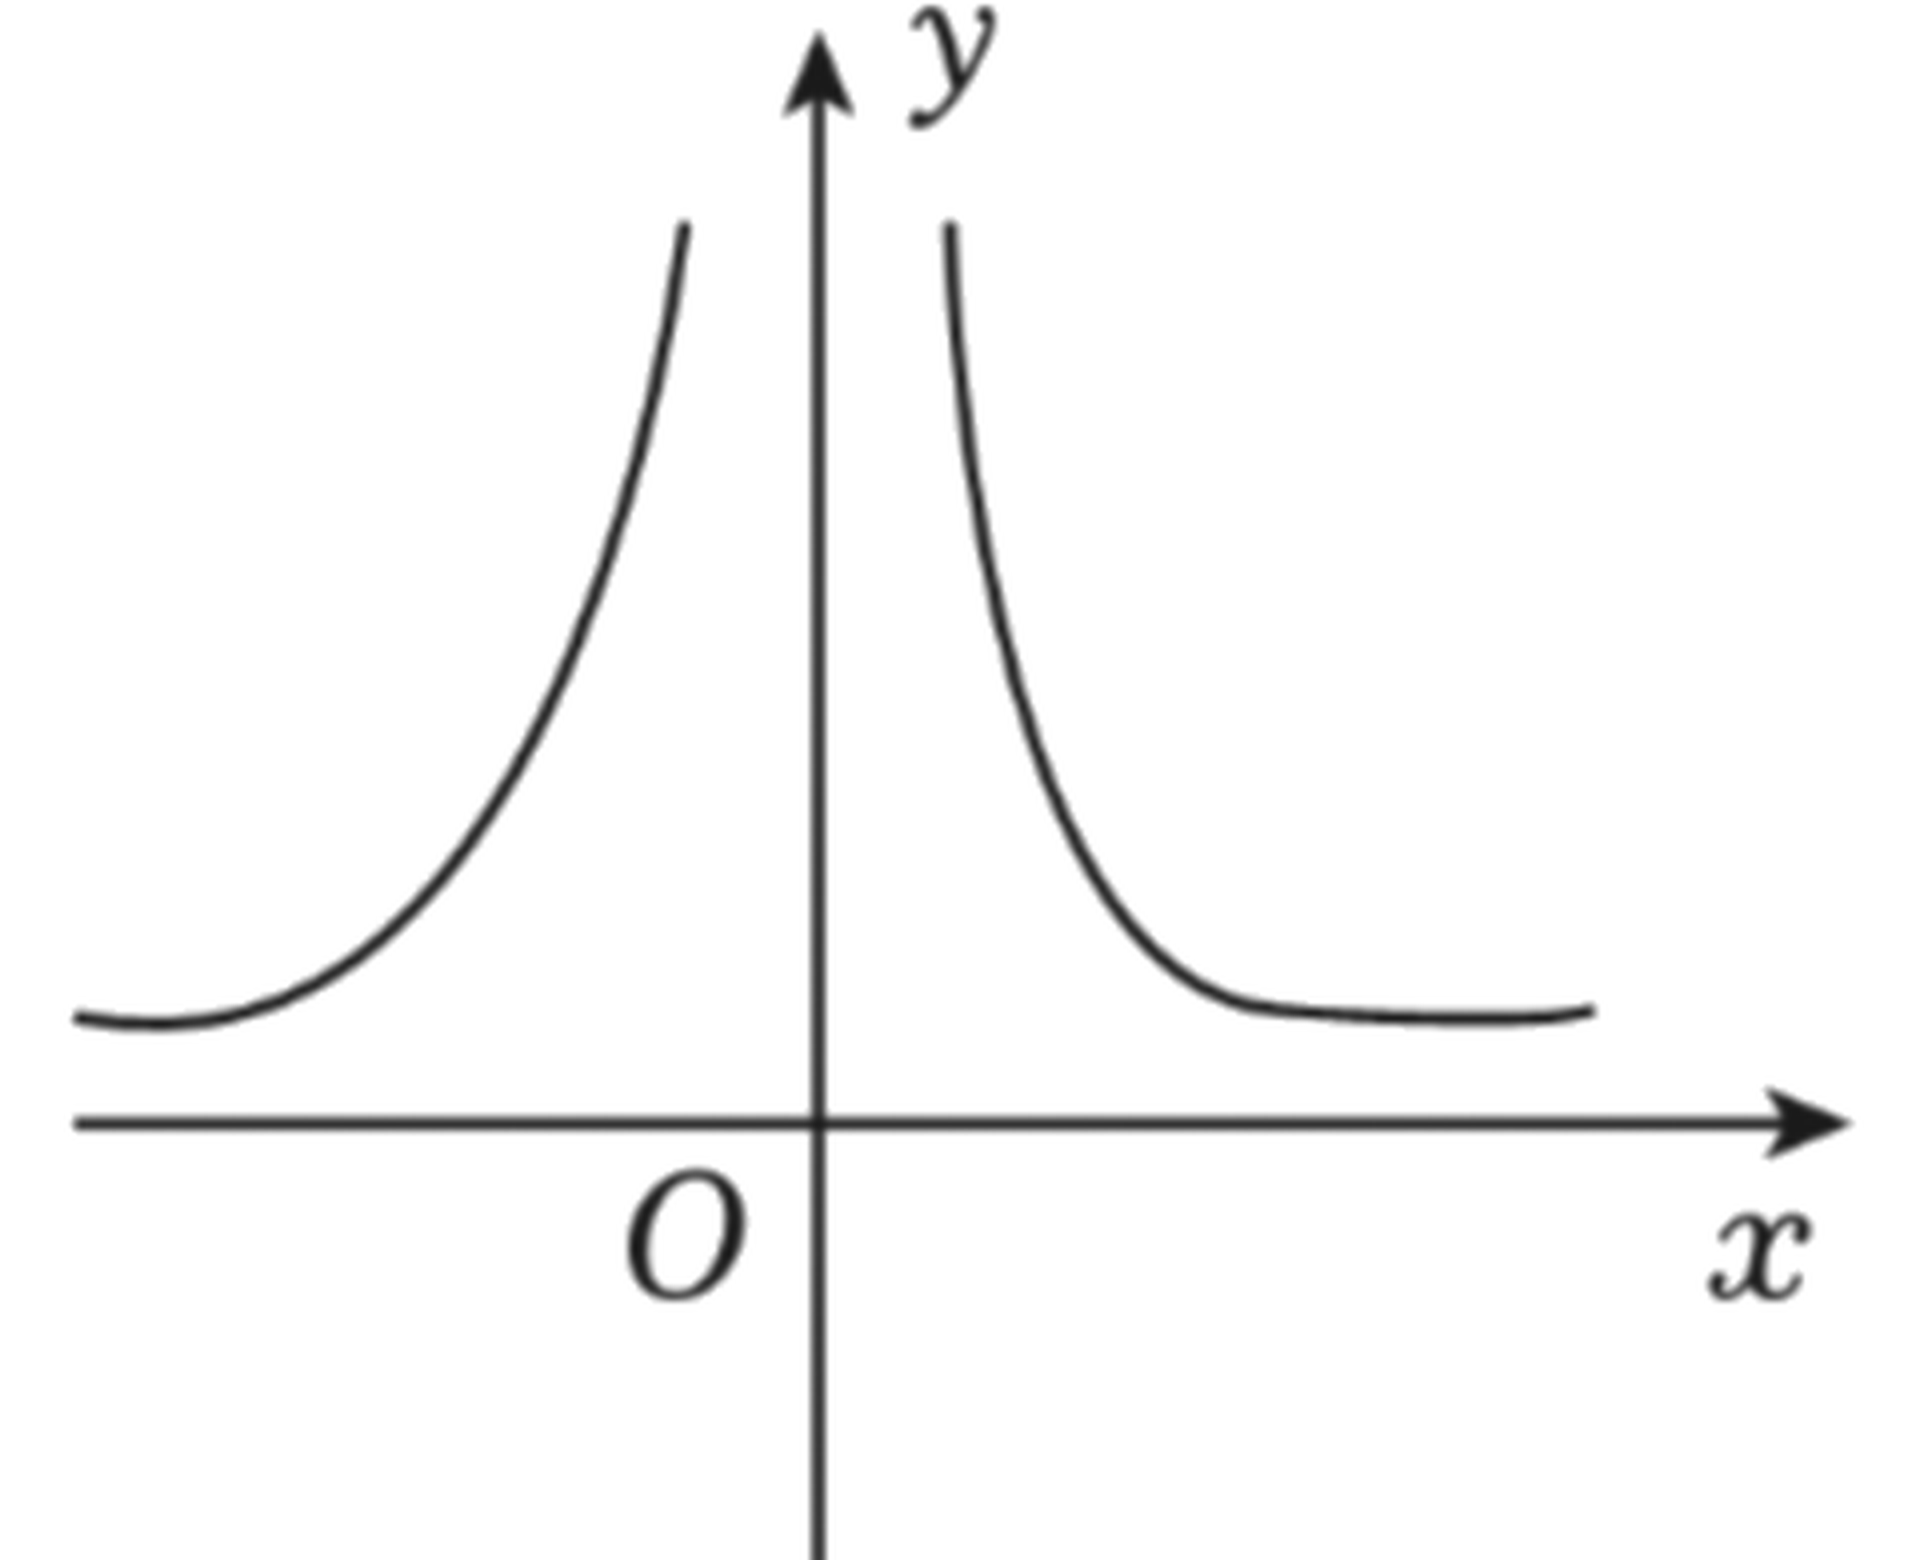
\includegraphics[width=0.36\textwidth]{figures/gao148_q16.png}
\end{center}

\ifanswer
\solbegin
\step{因为函数为偶函数，所以 $p$ 为偶数，且由图象形状判定 $\dfrac{p}{q}<0$.}
\step{又 $p$、$q$ 互质，所以 $q$ 为奇数. 故选 $D$.}
\solend
\fi

\end{enumerate}

\bigsec{三、解答题}

\begin{enumerate}
\setcounter{enumi}{16}

% === Q17 ===：\overline{B}／\varnothing／\R／\mid 逐处照录；解析 8 行
\item 已知集合 $A=\left\{x\mid \dfrac{5}{2x+1}>1\right\}$，$B=\{x\mid x^2+(a+3)x+3a<0,a\in\R\}$.

(1) 求 $A$.

(2) 若全集 $U=\R$，且 $A\cap\overline{B}=\varnothing$，求实数 $a$ 的取值范围.

\ifanswer
\solbegin
\step{(1) $\dfrac{5}{2x+1}>1$，即 $\dfrac{5}{2x+1}-1>0$，即 $\dfrac{4-2x}{2x+1}>0$，即 $(2x+1)(x-2)<0$，}
\step{解得 $-\dfrac{1}{2}<x<2$，所以 $A=\left(-\dfrac{1}{2},2\right)$；}
\step{(2) $x^2+(a+3)x+3a<0$，即 $(x+3)(x+a)<0$，}
\step{全集 $U=\R$，且 $A\cap\overline{B}=\varnothing$，}
\step{当 $a<3$ 时，解得 $-3<x<-a$，则 $\overline{B}=(-\infty,-3)\cup(-a,+\infty)$，}
\step{此时 $-a\geqslant2$，解得 $a\leqslant-2$，}
\step{当 $a\geqslant3$ 时，不满足 $A\cap\overline{B}=\varnothing$，}
\step{故实数 $a$ 的取值范围是 $(-\infty,-2]$.}
\solend
\fi

% === Q18 ===：cases 块整体算一个印刷行；解析 6 行
\item 已知幂函数经过点 $(2,4)$.

(1) 当 $x=\dfrac{1}{2}$ 时，求函数的值；

(2) 是否存在实数 $m$、$n$，使得该函数在区间 $[m,n]$ 上最小值为 $6m-8$，最大值为 $6n-8$？若存在，求出 $m$、$n$ 的值，若不存在，请说明理由.

\ifanswer
\solbegin
\step{(1) 设幂函数的解析式是 $y=x^\alpha$，则 $2^\alpha=4$，解得 $\alpha=2$，}
\step{故 $f(x)=x^2$，$f\left(\dfrac{1}{2}\right)=\dfrac{1}{4}$；}
\step{(2) 因为 $f(x)\geqslant0$，所以 $6m-8\geqslant0$，$m\geqslant\dfrac{4}{3}$，}
\step{由函数 $f(x)$ 在 $(0,+\infty)$ 严格增，得函数 $f(x)$ 在 $(m,n)$ 严格增，}
\step{所以 $\begin{cases}f(m)=6m-8\\f(n)=6n-8\end{cases}$ 且 $m<n$，解得 $m=2$，$n=4$，}
\step{故存在 $m=2$，$n=4$ 满足题意.}
\solend
\fi

% === Q19 ===：7 处评分档照 高一54／64 成例排 \dots\dots N 分；判别式高 \Delta；解析 9 行
\item 已知方程 $x^2+6mx+9m-2=0$，且 $x_1,x_2$ 是方程的两个不同的实数根.

(1) 若 $m=1$，求 $\dfrac{1}{x_1}+\dfrac{1}{x_2}$ 的值；

(2) 若 $m\in\R$，且 $x_1^2+x_2^2<4$，求 $m$ 取值范围.

\ifanswer
\solbegin
\step{(1) 当 $m=1$ 时，方程为 $x^2+6x+7=0$，\dots\dots1 分}
\step{则 $x_1+x_2=-6,x_1\cdot x_2=7$，\dots\dots2 分}
\step{$\dfrac{1}{x_1}+\dfrac{1}{x_2}=\dfrac{x_1+x_2}{x_1\cdot x_2}=-\dfrac{6}{7}$\dots\dots3 分}
\step{(2) $x_1+x_2=-6m,x_1\cdot x_2=9m-2$\dots\dots2 分}
\step{因为 $x_1^2+x_2^2=(x_1+x_2)^2-2x_1\cdot x_2$，所以 $(x_1+x_2)^2-2x_1\cdot x_2<4$，}
\step{所以 $36m^2-2(9m-2)<4$，解得 $0<m<\dfrac{1}{2}$\dots\dots2 分}
\step{又因为方程有两个不同的根，所以 $\Delta=36m^2-4(9m-2)>0$，}% 判别式原卷印等腰偏高粗三角 $\Delta$，照录（放大 07 页 q19_delta3.png／diag_band_q19.png 确认）
\step{解得 $m<\dfrac{1}{3}$ 或 $m>\dfrac{2}{3}$\dots\dots2 分}
\step{所以 $0<m<\dfrac{1}{3}$\dots\dots2 分}
\solend
\fi

% === Q20 ===：题目配图（矩形蔬菜温室，三版都出），\needvspace 守卫放 \item 之前；单位 \mathrm{m}／\mathrm{m}^2；解析 10 行
\needvspace{8cm}
\item 某村计划建造一个室内面积为 $600\mathrm{m}^2$ 的矩形蔬菜温室，在室内，沿左、右两侧与后侧内墙各保留 $2\mathrm{m}$ 宽的通道，沿前侧内墙保留 $4\mathrm{m}$ 宽的空地.

\begin{center}
% 矩形蔬菜温室示意图取 07 页右侧，去粉色水印、去色、4× LANCZOS 放大；三版都出
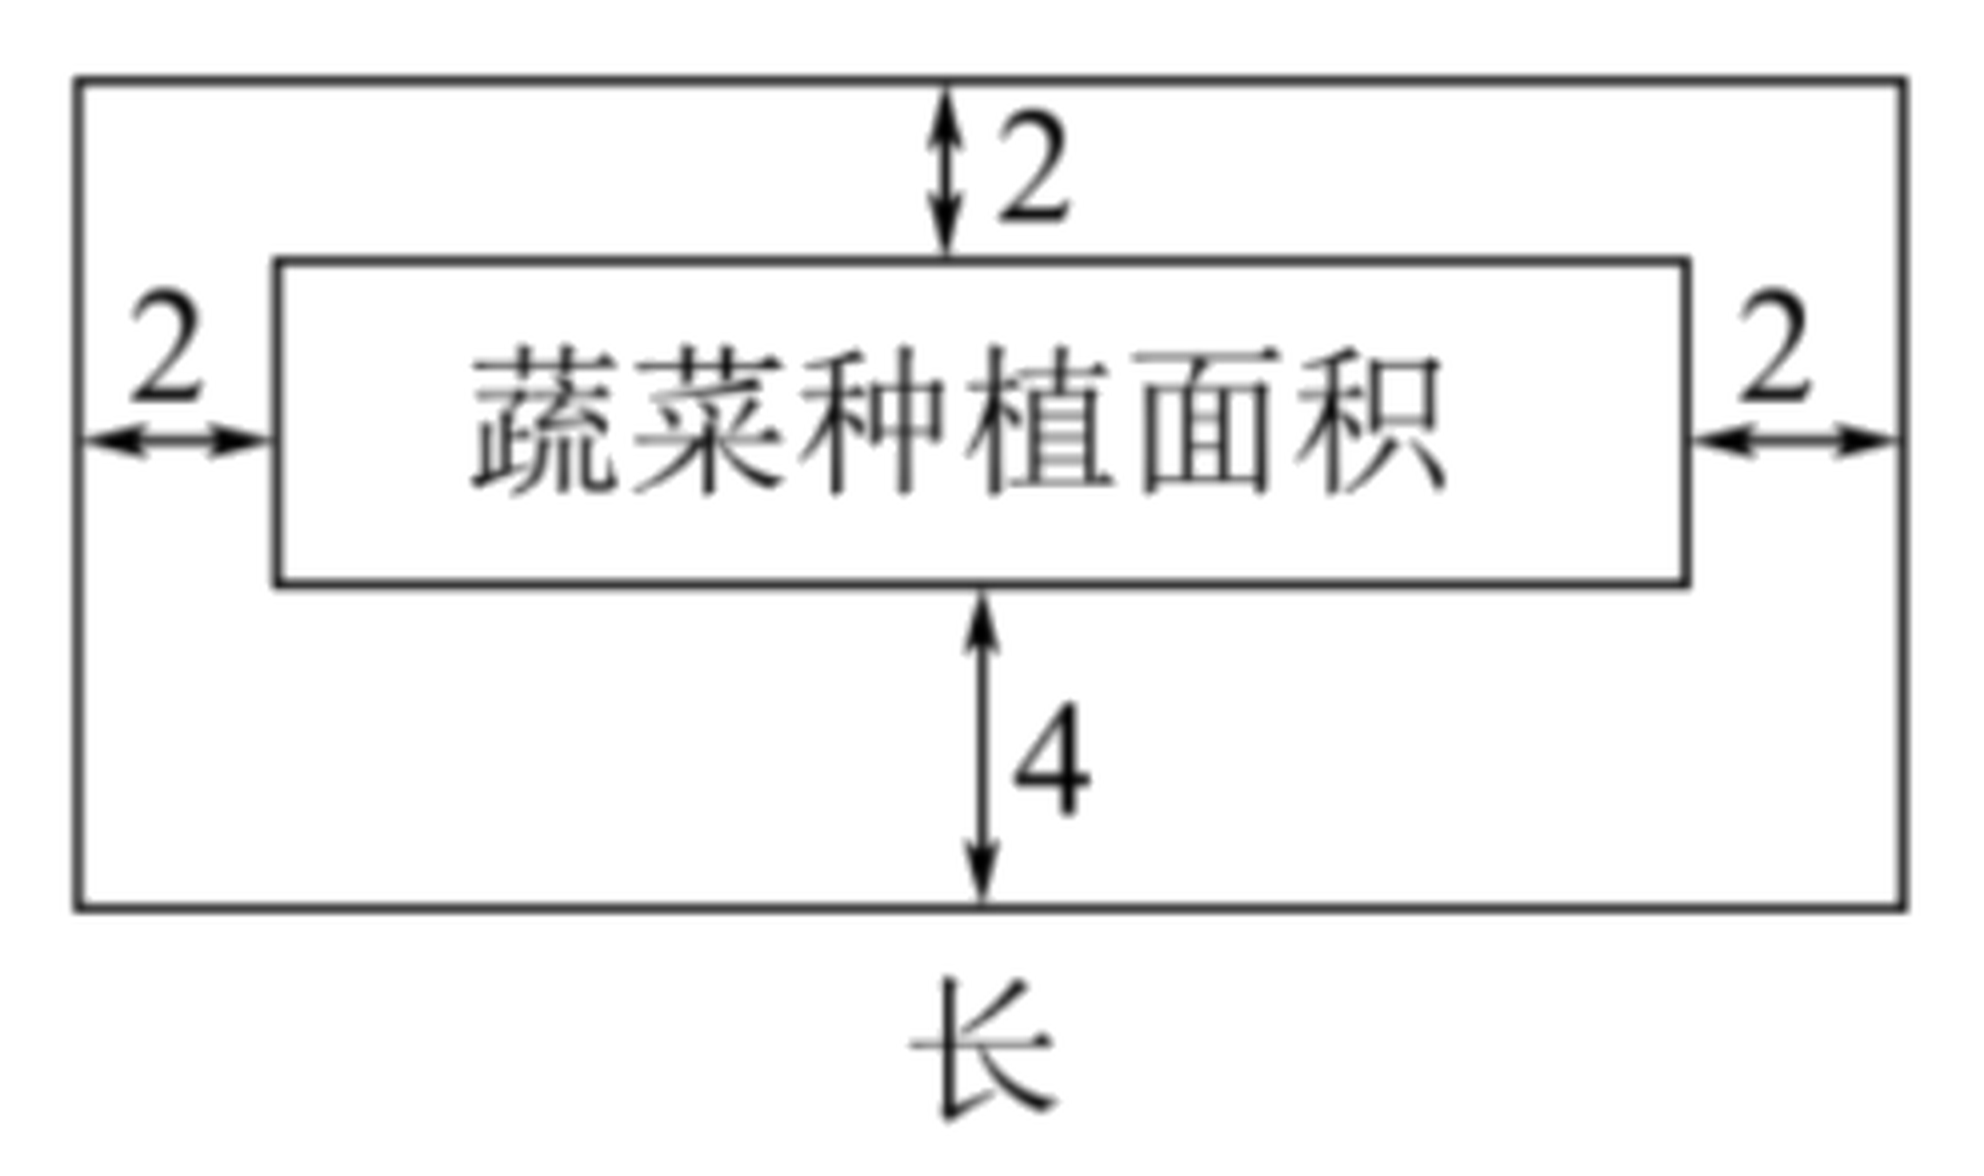
\includegraphics[width=0.45\textwidth]{figures/gao148_q20.png}
\end{center}

(1) 写出蔬菜的种植面积关于矩形温室的长之间的关系式.

(2) 当矩形温室的边长各为多少时，蔬菜的种植面积最大？最大种植面积是多少？

\ifanswer
\solbegin
\step{(1) 设蔬菜的种植面积为 $y\mathrm{m}^2$，矩形温室的长为 $x\mathrm{m}$，}
\step{则矩形温室的宽为 $\dfrac{600}{x}\mathrm{m}$，}
\step{种植蔬菜矩形的长为 $(x-4)\mathrm{m}$，宽为 $\left(\dfrac{600}{x}-6\right)\mathrm{m}$，}
\step{所以 $y=(x-4)\left(\dfrac{600}{x}-6\right)(4<x<100)$；}
\step{(2) 因为 $y=(x-4)\left(\dfrac{600}{x}-6\right)=624-\left(6x+\dfrac{2400}{x}\right)$，}
\step{因为 $6x+\dfrac{2400}{x}\geqslant2\sqrt{6x\cdot\dfrac{2400}{x}}=240$，}
\step{当且仅当 $6x=\dfrac{2400}{x}$，即 $x=20$ 时取等号，}
\step{所以 $y=624-\left(6x+\dfrac{2400}{x}\right)\leqslant624-240=384$.}
\step{即当矩形温室的一边长为 $20\mathrm{m}$，另一边长为 $30\mathrm{m}$ 时，}
\step{蔬菜的种植面积最大，最大为 $384\mathrm{m}^2$.}
\solend
\fi

% === Q21 ===：3 问、cases 块整体算一个印刷行；判别式高 \Delta；解析 19 行（末行续 09 页）
\item 二次函数 $f(x)=ax^2+bx+c$ 满足对任意的 $x\in\R$，$x-1\leqslant f(x)\leqslant x^2-x$ 恒成立.

(1) 求证：$f(1)$ 为定值；

(2) 若 $f(0)=-\dfrac{1}{4}$，求二次函数 $f(x)$ 的表达式；

(3) 求 $a+2b+5c$ 的取值范围.

\ifanswer
\solbegin
\step{(1) 对任意的 $x\in\R$，$x-1\leqslant f(x)\leqslant x^2-x$ 恒成立，则 $0\leqslant f(1)\leqslant0$，}
\step{所以 $f(1)=0$，为定值.}
\step{(2) 由(1)得 $a+b+c=f(1)=0$，由 $f(0)=-\dfrac{1}{4}$，得 $c=-\dfrac{1}{4}$，}
\step{则 $b=\dfrac{1}{4}-a$，$f(x)=ax^2+\left(\dfrac{1}{4}-a\right)x-\dfrac{1}{4}$，}
\step{不等式 $x-1\leqslant f(x)$ 可化为 $ax^2+\left(\dfrac{1}{4}-a\right)x-\dfrac{1}{4}\geqslant x-1$，}
\step{即 $ax^2-\left(a+\dfrac{3}{4}\right)x+\dfrac{3}{4}\geqslant0$，}
\step{一元二次不等式 $ax^2-\left(\dfrac{3}{4}+a\right)x+\dfrac{3}{4}\geqslant0$ 恒成立，则 $\begin{cases}a>0\\\Delta=\left(a+\dfrac{3}{4}\right)^2-3a\leqslant0\end{cases}$，}% 判别式原卷印等腰偏高粗三角 $\Delta$，照录（放大 08 页 q21_delta3.png／diag_band_q21.png 确认）
\step{解得 $a=\dfrac{3}{4}$，}
\step{此时 $f(x)=\dfrac{3}{4}x^2-\dfrac{1}{2}x-\dfrac{1}{4}$，$x^2-x-f(x)=\dfrac{1}{4}(x-1)^2\geqslant0$ 恒成立，}
\step{所以 $f(x)=\dfrac{3}{4}x^2-\dfrac{1}{2}x-\dfrac{1}{4}$.}
\step{(3) 由(1)得 $b=-a-c$，$f(x)=ax^2-(a+c)x+c=(ax-c)(x-1)$，}
\step{不等式 $x-1\leqslant f(x)$ 可化为 $(x-1)(ax-c-1)\geqslant0$，}
\step{一元二次不等式 $(x-1)(ax-c-1)\geqslant0$ 恒成立，则 $a>0$，}
\step{且方程 $(x-1)(ax-c-1)=0$ 有相等的实数根，因此 $c=a-1$，$a>0$，}
\step{不等式 $f(x)\leqslant x^2-x\Leftrightarrow(ax-c)(x-1)\leqslant x^2-x\Leftrightarrow(x-1)[(1-a)x+c]\geqslant0$，}
\step{同理 $1-a>0$，且方程 $(x-1)[(1-a)x+c]=0$ 有相等的实数根，}
\step{因此 $c=a-1$，$a<1$，从而 $c=a-1$，$b=1-2a$，$0<a<1$，}
\step{$a+2b+5c=a+2(1-2a)+5(a-1)=2a-3\in(-3,-1)$，}
\step{所以 $a+2b+5c$ 的取值范围是 $(-3,-1)$.}
\solend
\fi

\end{enumerate}

\end{document}
"
% 紧凑版：xelatex "\def\iscompact{1}% 高一148_新川中学_期中.tex
%   —— 高一上数学"2026-2027 年新川中学高一上期中"（试卷版/答案版/紧凑版）
% 试卷版：xelatex 高一148_新川中学_期中.tex
% 答案版：xelatex "\def\isanswer{1}% 高一148_新川中学_期中.tex
%   —— 高一上数学"2026-2027 年新川中学高一上期中"（试卷版/答案版/紧凑版）
% 试卷版：xelatex 高一148_新川中学_期中.tex
% 答案版：xelatex "\def\isanswer{1}\input{高一148_新川中学_期中.tex}"
% 紧凑版：xelatex "\def\iscompact{1}\input{高一148_新川中学_期中.tex}"
%
% ① 原始材料：微信公众号"魔都数学加油站"文章，连载"27学年高一148"，原文标题
% "27学年高一148——2026-2027年上海市新川中学高一上期中"（2026-11-21 推送）；
% 原文链接：https://mp.weixin.qq.com/s/Alhmwb3sSLQMp_wjzoAVyA 。
% 正文为 9 张 PNG 页（01/03/04/07/08/09 为 2560×3620，02/05/06 为 4762×6735，
% 同一篇各页分辨率混排，逐页按各自分辨率裁图核对，别按预览比例换算裁框）。
% 体例：混合体例讲评版——19 题中 Q4、Q5 只印【答案】、无【解析】；Q13 的答案"C"
% 直接印在题干括号内、无【答案】/【解析】段；其余 16 题印【解析】（逐题核实，见 ② ②）。
% 题目、答案、解析均据原图转录；卷面粉红色水印"魔都数学加油站"及公众号页脚未录入。
% 全卷插图清单（逐页通读 9 页确认）：4 幅题目配图，均三版都出、均非【解析】内配图：
%   · Q12 幂函数曲线族图（03 页右侧：x/y 轴、O、A(1,0)、B(0,1)、M、N 与两族
%     y=x^α／y=x^β 曲线、线段 AB、虚线），题干"（如图）"处，裁 figures/gao148_q12.png；
%   · Q15 四条指数函数曲线图（04 页右侧：①②③④ 四曲线同过 (0,1)、x/y 轴、O、
%     y 轴刻度 1），题干"如图"处，裁 figures/gao148_q15.png；
%   · Q16 关于 y 轴对称的幂函数曲线图（04 页右下：x/y 轴、O、两支上翘曲线），
%     题干"如图所示"处，裁 figures/gao148_q16.png；
%   · Q20 矩形蔬菜温室示意图（07 页右侧：大矩形＋内框"蔬菜种植面积"＋2/2/4
%     通道标注＋"长"），题干处，裁 figures/gao148_q20.png；
%   其余各页逐页确认无其它题目配图、无【解析】内配图、无表格，亦无"题干写如图而
%   源码漏图"一处；Q19 解析行末的虚线"----N 分"为评分档（非图），Q18／Q21 的
%   cases 块为数学块（非图）。4 图均取自原卷截图，去粉色水印、去色、4× LANCZOS 放大。
%
% 卷首标题：原卷印作"2026-2027 年新川中学高一上期中"，年份区间按全稿惯例排 en dash；
% 原卷卷面未印副标题，本稿按同期中卷（高一140／141／143／144／145／146／147）知识模块
% 口径补出"集合与常用逻辑用语、不等式、函数"。
%
% 题号体例（逐页核实定稿）：本卷共 19 题——一、填空题 3—12（10 题）、
% 二、选择题 13—16（4 题）、三、解答题 17—21（5 题）。
% 三节分别 \setcounter{enumi}{2}／{12}／{16}。原卷从第 3 题起、无第 1、2 题，
% 本稿保留原题号；全卷无附加题节、无 Q22（Q21 解析末行"所以 a+2b+5c 的取值范围是
% (-3,-1)."为全卷收尾，09 页下半仅水印、无正文）。
%
% ② 与原卷的排版差异：
%   ① 原文从第 3 题起，本稿保留原题号；共 19 题三节；
%   ② 混合体例逐题核实：Q4（反证法"假设的内容"）、Q5 只印【答案】、无【解析】，
%      按 高一140 第 5 题／高一145 Q3 成例提 \ans{}、不补造解析；Q13 答案"C"直接
%      印在题干括号内（" ( C ) "）、全卷无该题【答案】/【解析】段，按 高一84 Q13／
%      高一37 Q13／高一53 Q13 成例括号 \mbox{（\quad）} 留空、另提 \ans{$C$}；
%      其余 16 题印【解析】、用 \solbegin…\solend，选择题答案在解析末句"故选 X"
%      （Q14 选 D、Q15 选 B、Q16 选 D，逐个放大原图核实）、题干括号留空、不另提
%      \ans{}；答案版【答案】/【解析】标记数 = 19（3 个 \ans ＋ 16 个 \solbegin）
%      = 全卷题数；
%   ③ 原卷卷面未印副标题，本稿按知识模块口径补出；
%   ④ 原卷填空横线按全稿惯例排 \blankline[4.4em]；选择题括号排 \mbox{（\quad）}、
%      选项段前按惯例加 \keepwithprev；Q13／Q16 四选项为两行两列、Q14／Q15 选项
%      为一行，照原卷分行；解答题不留作答区、不加 \anspace（原卷为讲评版，
%      与 129／131／132／133／136／140／141／143／144／145／146 同）；
%   ⑤ 数集：Q11"在 R 上定义运算"、Q13"x、y∈R"、Q16"p、q∈Z"、Q17"a∈R"
%      "U=R"、Q19"m∈R"、Q21"x∈R" 原卷印斜体 R/Z，按全稿惯例统一改 \R／\Z
%      （本卷未出现 N，\N^* 无对应处）；绝对值排 \lvert…\rvert（Q9／Q14），
%      集合描述竖线排 \mid（Q17）；不等号按全稿惯例排 \leqslant／\geqslant；
%      补集照原卷上划线排 \overline{B}（Q17 题干 1 处＋解析 3 处）；空集
%      \varnothing（Q17 题干 1 处＋解析 2 处）；\subset（Q3 题干 {a}⊂M）与
%      \subseteq（Q3 题干 M⊆{a,b,c,d}）逐处照录不统一（放大 01 页 q3_subset.png）；
%   ⑥ 子题标号 (1)(2)(3) 半角括号照录；圈数字 ①—⑥ 在文本模式（Q14 六个结论、
%      Q15 曲线编号与其解析、Q14 解析"对①…对⑥"），按 common.sty 划入 CJK 字符类
%      渲染；cases 块整体算一个印刷行；\left…\right 不得拆到不同 $…$ 组；
%      单位 m／m² 排 \mathrm{m}／\mathrm{m}^2（Q20，原卷印正体 m）；
%   ⑦ 题干／解析中的中文弯引号按原卷照录：Q4" ab 可以被 5 整除，那么 a、b 中
%      至少有一个能被 5 整除 "（开引号后有空格、闭引号后空格接"时"）、
%      Q13" x=0 "" xy=0 "（引号内空格），注释内一律 ASCII 引号；
%   ⑧ 半角逗号在数学组之间是全稿惯例、非笔误（Q3"{a,b,c,d}"、Q6"$x,y$"
%      "$x=\frac13,y=\frac16$"、Q10、Q11"$a=-2,b=-1"、Q12"$\alpha=\log..,\beta=..$"、
%      Q14"$a+b<0,a-b<0$"、Q17、Q19"$x_1+x_2=-6,x_1\cdot x_2=7$"、Q20、Q21 等），
%      逐处照录别改全角；行末西文句点照录为 ASCII `.`；行中全角逗号／顿号照录；
%   ⑨ "图像／图象"逐处放大核：全卷 9 处均印"图象"（象，无亻）、未见"图像"，
%      逐处照录未统一改动（Q8 题干/解析各 1、Q12 题干 2、Q15 题干 1／解析 2、
%      Q16 题干 1／解析 1；放大 02/03/04/05 页 /tmp/gao148/zoom/my_wide_a.png、
%      my_wide_b.png 与宋体参考"象／像"并排确认）；
%   ⑩ 判别式 Δ/△ 混用是照录项：Q11 解析"△=1−4(−a²+a+1)<0"印扁等边空心
%      三角 \triangle；Q19 解析"Δ=36m²−4(9m−2)>0"、Q21 解析 cases 块
%      "Δ=(a+3/4)²−3a≤0" 两处印等腰偏高粗三角 \Delta，逐处放大判断、照录
%      不统一（参照 高一142／144／145 头注④口径，详见 ④）；
%   ⑪ 一条 \step = 原卷解析的一个印刷行，cases 块整体算一个印刷行；别把原卷折行
%      并起来、别把一行拆多条。Q3 六行、Q7 五行（01 页末首行＋02 页顶四行）、
%      Q9 七行、Q11 五行、Q14 八行（对② 的两行公式各占一印刷行）、Q17 八行、
%      Q18 六行、Q19 九行（7 处评分档附在行末）、Q20 十行、Q21 十九行
%      均按印刷行逐条断，不丢行；
%   ⑫ 配图：4 幅均为题目配图（三版都出），放 \item 内题干之后 \begin{center}；
%      大图块加 \needvspace 守卫把整块推走（守卫放 \item 之前，见 高一145 Q14/Q20
%      成例与切页审计 B 类坑）；三版切页审计均"合计异常：无"；
%   ⑬ 跨页续印按题合并：Q3/4/5 在 01 页；Q6 题干＋解析在 01 页；Q7 题干在 01 页
%      末、解析首行在 01 页末续 02 页顶四行；Q8/9/10 在 02 页（Q9 解析续 02 页下半、
%      Q10 题干与解析前 2 行在 02 页末）；Q10 解析末行续 03 页顶；Q11/12 在 03 页、
%      "二、选择题"标题与 Q13/14 题干在 03 页下半；Q13 无解析；Q14 解析在 04 页顶、
%      Q15 题干＋图＋选项＋解析在 04 页、Q16 题干＋图在 04 页末；Q16 选项＋解析＋
%      "三、解答题"标题＋Q17 题干＋解析在 05 页、Q18 题干首句在 05 页末；Q18 题干
%      续＋解析、Q19 题干＋解析前 5 行在 06 页；Q19 解析续 4 行＋Q20 题干＋图＋
%      解析（10 行全部）在 07 页，末行"蔬菜的种植面积最大，最大为 384m²."收尾；
%      Q21 题干＋解析前 18 行在 08 页；Q21 解析末行"所以 a+2b+5c 的取值范围是
%      (-3,-1)."在 09 页上半（09 页下半仅水印、无正文）。本稿按题连排，不丢行、
%      不并折行；
%   ⑭ 原卷解析内无红色"法一／法二"之类小标题，故本卷无 \stepm；水印
%      "魔都数学加油站"红色不录入；Q19 解析 7 处评分档（1/2/3/2/2/2/2 分）
%      原卷在行末印一串虚线，本稿照 高一54／64 成例排 \dots\dots N 分，
%      分值逐处照录、位置不变。
%
% ③ 行数复核：一条 \step／\stepm = 原卷解析的一个印刷行，cases 块作一个印刷行计。
%   逐题数（主会话逐页核对定稿）：Q3：6；Q4：0（只印【答案】、提 \ans{}）；
%   Q5：0（只印【答案】、提 \ans{}）；Q6：2；Q7：5；Q8：2；Q9：7；Q10：3；
%   Q11：5；Q12：2；Q13：0（答案印在题干括号内、另提 \ans{}）；Q14：8；Q15：5；
%   Q16：2；Q17：8；Q18：6；Q19：9；Q20：10；Q21：19。
%   合计 99 条 \step（本卷无 \stepm：解析内无红色"法一／法二"类小标题），
%   与原卷逐题印刷行相等。全卷 16 题设 \solbegin…\solend ＋ 3 处 \ans{}，
%   答案版【答案】/【解析】标记数 = 19 = 全卷题数。
%
% ④ 判别式／子集符号结论（逐处放大原图照录、不得统一，主会话像素级复核）：
%   判别式全卷 3 处，两形混用逐处照录不统一（参照 高一142／144／145 头注④口径）：
%     · Q11 解析"△=1−4(−a²+a+1)<0" 原卷印扁等边空心三角（宽>高、细线），
%       照录 \triangle（放大 03 页 /tmp/gao148/zoom/q11_delta3.png、
%       delta_montage.png 确认）；
%     · Q19 解析"Δ=36m²−4(9m−2)>0" 原卷印等腰偏高粗三角（高>宽），
%       照录 \Delta（放大 07 页 /tmp/gao148/zoom/q19_delta3.png 确认）；
%     · Q21 解析 cases 块"Δ=(a+3/4)²−3a≤0" 原卷印等腰偏高粗三角（高>宽），
%       照录 \Delta（放大 08 页 /tmp/gao148/zoom/q21_delta3.png 确认）。
%   子集／补集：Q3 题干"{a}⊂M⊆{a,b,c,d}" 前者印单线 ⊂、无下划线，照录 \subset；
%     后者印带下划线 ⊆，照录 \subseteq（放大 01 页 /tmp/gao148/zoom/q3_subset.png
%     确认）；Q17 题干 1 处＋解析 3 处共 4 处 \overline{B} 照原卷上划线
%     （B 上横线、非 C_U B）；空集 \varnothing 3 处（Q17 题干 1 处、解析 2 处）；
%     Q17 集合描述竖线 \mid；数集 \R／\Z 归一见 ② ⑤。
%
% ⑤ 存疑照录（放大原图确认，照录未改、正文对应处另有 % 注）：
%   1. Q3 解析末行"所以 M 一共有 3+3+1+1=8 个" 原卷印 $3+3+1+1=8$，按上文
%      四行应为 $1+3+3+1=8$（疑为原卷加数顺序笔误，和仍为 8），放大 01 页
%      /tmp/gao148/zoom/my_q3_sol.png 确认，照录未改。
%   2. Q13 答案"C"直接印在题干括号内、全卷无该题【答案】/【解析】段，按
%      高一84 Q13 成例括号留空、另提 \ans{$C$}（见 ② ②），未补造解析。
%   3. Q19 解析 7 处评分档（"----N 分"）原卷印一串虚线，本稿照 高一54／64
%      成例排 \dots\dots N 分，分值逐处照录、位置不变。
%   4. 判别式 Q11 扁 \triangle 与 Q19／Q21 高 \Delta 两形混用，逐处照录不统一（见 ④）。
%   5. "图像／图象"全卷 9 处均印"图象"、未见"图像"（见 ② ⑨），逐处放大核实照录，
%      未统一改动。
%   全卷除此 5 类外未发现其它笔误／自相矛盾处。
%
% ⑥ 跨页续印按题合并说明：见 ② ⑬。
%
\documentclass[a4paper,11pt]{article}
\usepackage{common}

\begin{document}

\examtitlest[3]{2026--2027 年新川中学高一上期中}{集合与常用逻辑用语、不等式、函数}

\bigsec{一、填空题}

\begin{enumerate}
\setcounter{enumi}{2}

% === Q3 ===：题干 {a}⊂M⊆{a,b,c,d} 两个子集符号逐处照录；解析 6 行
\item 满足 $\{a\}\subset M\subseteq\{a,b,c,d\}$ 的集合 $M$ 有\blankline[4.4em]个.

\ifanswer
\solbegin
\step{$M$ 是 $\{a,b,c,d\}$ 的子集，但必含有元素 $a$，}
\step{当 $M$ 中只一个元素时，$M=\{a\}$ 只有 1 个；}
\step{当 $M$ 中有二个元素时，$M$ 有 3 个；}
\step{当 $M$ 中有三个元素时，$M$ 有 3 个；}
\step{当 $M$ 中有四个元素时，$M$ 有 1 个；}
\step{所以 $M$ 一共有 $3+3+1+1=8$ 个.}% 原卷印 $3+3+1+1=8$（按上文四行应为 $1+3+3+1$），疑为加数顺序笔误，照录未改（放大 01 页 my_q3_sol.png）
\solend
\fi

% === Q4 ===：原卷只印【答案】、无【解析】，按 高一140 第 5 题成例提 \ans{}；弯引号与空格照录
\item 用反证法证明命题 “ $ab$ 可以被 5 整除，那么 $a$、$b$ 中至少有一个能被 5 整除” 时假设的内容应该是\blankline[4.4em].

\ifanswer
\ans{$a$、$b$ 都不能被 5 整除}
\fi

% === Q5 ===：原卷只印【答案】 $[-2,1)$、无【解析】，提 \ans{}
\item 不等式 $\dfrac{x+2}{x-1}\leqslant0$ 的解集为\blankline[4.4em].

\ifanswer
\ans{$[-2,1)$}
\fi

% === Q6 ===：解析 2 行；半角逗号在数学组之间照录
\item 设 $x,y\in(0,+\infty)$，且 $x+4y=1$，则 $\dfrac{1}{x}+\dfrac{1}{y}$ 的最小值为\blankline[4.4em].

\ifanswer
\solbegin
\step{因为 $\dfrac{1}{x}+\dfrac{1}{y}=(x+4y)\left(\dfrac{1}{x}+\dfrac{1}{y}\right)=5+\dfrac{4y}{x}+\dfrac{x}{y}\geqslant5+2\sqrt{\dfrac{4y}{x}\cdot\dfrac{x}{y}}=9$，}
\step{当且仅当 $\dfrac{4y}{x}=\dfrac{x}{y}$，即 $x=2y$，即 $x=\dfrac{1}{3},y=\dfrac{1}{6}$ 时取等号，故最小值为 9.}
\solend
\fi

% === Q7 ===：题干在 01 页末、解析首行在 01 页末续 02 页顶四行；解析 5 行
\item 若不等式 $x^2+ax+b<0$ 的解集为 $(-3,-1)$，则不等式 $bx^2+ax+1\leqslant0$ 的解集为\blankline[4.4em].

\ifanswer
\solbegin
\step{不等式 $x^2+ax+b<0$ 的解集为 $(-3,-1)$，}
\step{所以方程 $x^2+ax+b=0$ 的两个实数根为 $-3$ 和 $-1$，}
\step{由根与系数的关系得 $a=4$，$b=3$，}
\step{故 $bx^2+ax+1\leqslant0$ 可化为 $3x^2+4x+1\leqslant0$，解得 $-1\leqslant x\leqslant-\dfrac{1}{3}$，}
\step{所求不等式 $bx^2+ax+1\leqslant0$ 的解集为 $\left[-1,-\dfrac{1}{3}\right]$.}
\solend
\fi

% === Q8 ===："图象"照录；解析 2 行
\item 函数 $y=a^{x-2}+2(a>0,a\ne1)$ 的图象必经过定点\blankline[4.4em].

\ifanswer
\solbegin
\step{令 $x-2=0$，得 $x=2$，则 $y=a^0+2=3$，}
\step{所以函数 $y=a^{x-2}+2$ 的图象过定点 $(2,3)$.}
\solend
\fi

% === Q9 ===：解析 7 行；首句末西文句点照录
\item 不等式 $\lvert x+3\rvert+\lvert a-x\rvert>6$ 对一切实数 $x$ 恒成立，则实数 $a$ 的取值范围为\blankline[4.4em].

\ifanswer
\solbegin
\step{$\lvert x+3\rvert$ 表示 $x$ 到 $-3$ 的距离，$\lvert a-x\rvert$ 表示 $x$ 到 $a$ 的距离.}
\step{所以它们的和为 $x$ 到 $-3$ 和 $x$ 到 $a$ 的距离之和，}
\step{当 $x$ 位于 $-3$ 和 $a$ 之间时，距离和取得最小值，}
\step{即两点之间的距离 $\lvert a-(-3)\rvert=\lvert a+3\rvert$，}
\step{若最小值 $\lvert a+3\rvert>6$，则原式对所有 $x$ 恒成立.}
\step{解得 $a+3>6$ 或 $a+3<-6$，即 $a>3$ 或 $a<-9$，}
\step{故 $a\in(3,+\infty)$ 或 $a\in(-\infty,-9)$.}
\solend
\fi

% === Q10 ===：题干与解析前 2 行在 02 页末、解析末行续 03 页顶；解析 3 行
\item 已知 $2^a=3$，$\log_3 5=b$，则 $\log_{15}20=$\blankline[4.4em]（用 $a$、$b$ 表示）.

\ifanswer
\solbegin
\step{因为 $2^a=3$，所以 $a=\log_2 3=\dfrac{\lg3}{\lg2}$，又 $\log_3 5=b=\dfrac{\lg5}{\lg3}$，}
\step{所以 $\lg3=a\lg2$，$\lg5=b\lg3=ba\lg2$，}
\step{则 $\log_{15}20=\dfrac{2\lg2+\lg5}{\lg3+\lg5}=\dfrac{2\lg2+ab\lg2}{a\lg2+ab\lg2}=\dfrac{2+ab}{a+ab}$.}
\solend
\fi

% === Q11 ===：在 \R 上定义运算 \otimes；判别式扁 \triangle 照录；解析 5 行
\item 在 $\R$ 上定义运算 $\otimes:x\otimes y=x(1-y)$，若不等式 $(x-a)\otimes(x+a)<1$ 对任意实数 $x$ 恒成立，则 $a$ 的取值范围是\blankline[4.4em].

\ifanswer
\solbegin
\step{由题意得不等式 $(x-a)\otimes(x+a)<1$ 对任意实数 $x$ 恒成立，}
\step{即不等式 $(x-a)(1-x-a)<1$ 对任意实数 $x$ 恒成立，}
\step{即 $x^2-x-a^2+a+1>0$ 对任意实数 $x$ 恒成立，}
\step{所以 $\triangle=1-4(-a^2+a+1)<0$，解得 $-\dfrac{1}{2}<a<\dfrac{3}{2}$，}% 判别式原卷印扁等边空心三角 $\triangle$，照录（放大 03 页 q11_delta3.png 确认）
\step{所以实数 $a$ 的取值范围为 $\left(-\dfrac{1}{2},\dfrac{3}{2}\right)$.}
\solend
\fi

% === Q12 ===：题目配图（幂函数曲线族，三版都出）；"图象"照录；解析 2 行
\needvspace{8cm}
\item 幂函数 $y=x^\alpha$，当 $\alpha$ 取不同的正数时，在区间 $[0,1]$ 上它们的图象是一族美丽的曲线（如图）. 设点 $A(1,0)$，$B(0,1)$，连接 $AB$，线段 $AB$ 恰好被其中的两个幂函数 $y=x^\alpha$，$y=x^\beta$ 的图象三等分，即有 $BM=MN=NA$，那么 $\alpha\beta=$\blankline[4.4em].

\begin{center}
% 幂函数曲线族图取 03 页右侧，去粉色水印、去色、4× LANCZOS 放大；三版都出
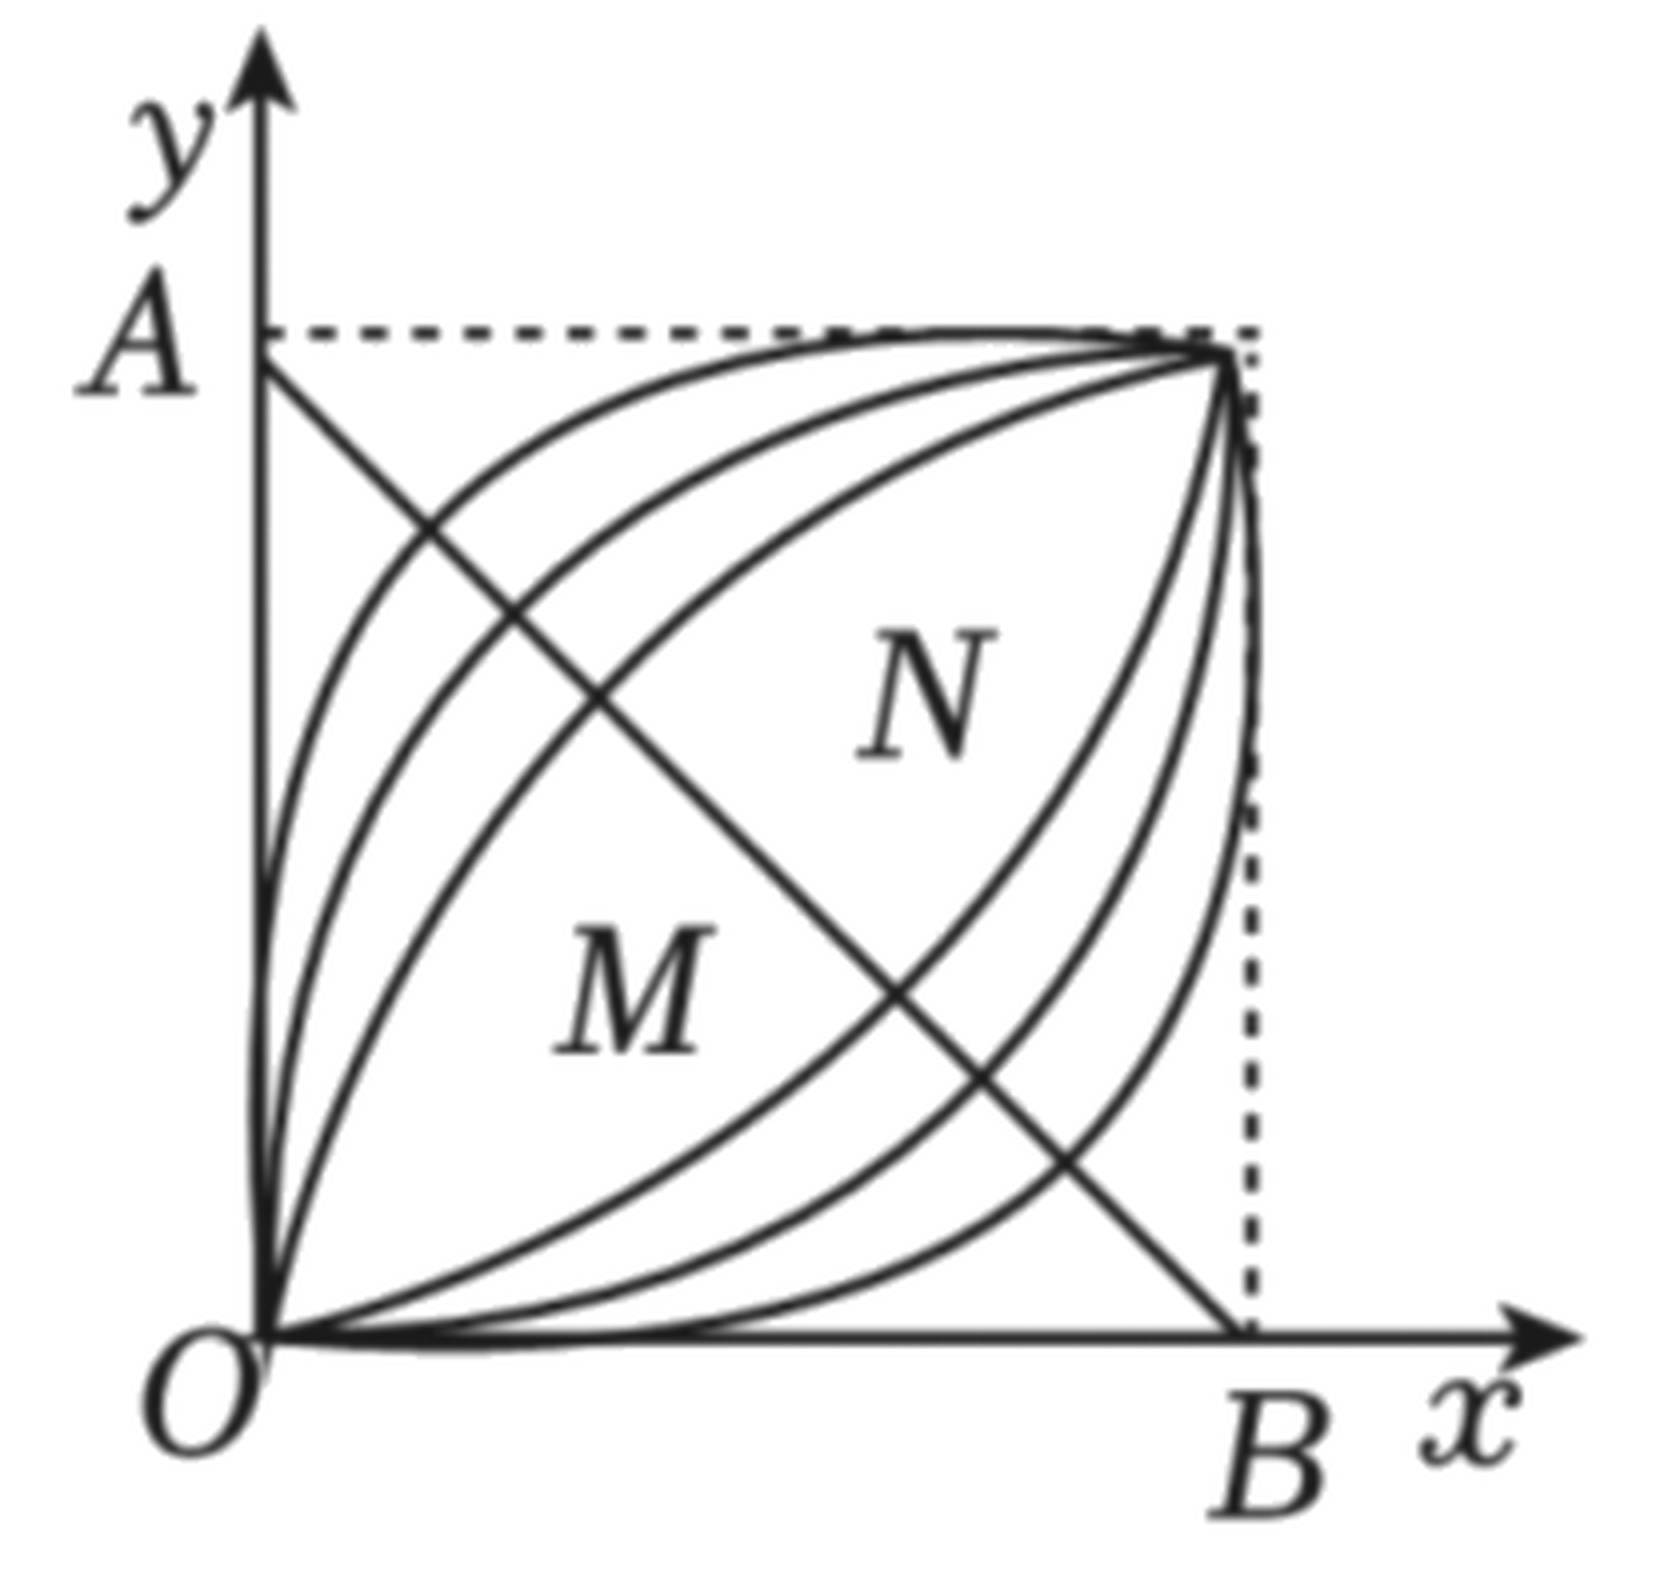
\includegraphics[width=0.40\textwidth]{figures/gao148_q12.png}
\end{center}

\ifanswer
\solbegin
\step{$BM=MN=NA$，点 $A(1,0)$，$B(0,1)$，所以 $M\left(\dfrac{1}{3},\dfrac{2}{3}\right)$，$N\left(\dfrac{2}{3},\dfrac{1}{3}\right)$，}
\step{分别代入 $y=x^\alpha$，$y=x^\beta$，$\alpha=\log_{\frac{2}{3}}\dfrac{1}{3},\beta=\log_{\frac{1}{3}}\dfrac{2}{3}$，$\alpha\beta=\log_{\frac{1}{3}}\dfrac{2}{3}\cdot\log_{\frac{2}{3}}\dfrac{1}{3}=1$.}
\solend
\fi

\end{enumerate}

\bigsec{二、选择题}

\begin{enumerate}
\setcounter{enumi}{12}

% === Q13 ===：答案"C"直接印在题干括号内、全卷无该题【答案】/【解析】段，按 高一84 Q13 成例括号留空、另提 \ans{$C$}；弯引号含空格
\item 若 $x$、$y\in\R$，则 “ $x=0$ ” 是 “ $xy=0$ ” 的\mbox{（\quad）}

\keepwithprev
A. 充要条件\qquad\qquad B. 必要不充分条件

C. 充分不必要条件\qquad\qquad D. 既不充分也不必要条件

\ifanswer
\ans{$C$}
\fi

% === Q14 ===：六个结论（圈数字在文本模式）、四选项一行；解析 8 行（对② 的两行公式各占一印刷行）
\item 若 $a<b<0$，下面有六个结论：① $a^2>b^2$；② $a^3<b^3$；③ $\dfrac{1}{a}<\dfrac{1}{b}$；④ $\dfrac{a}{b}>1$；⑤ $\dfrac{1}{a-b}>\dfrac{1}{a}$；⑥ $\lvert a\rvert>-b$. 其中正确的个数是\mbox{（\quad）}

\keepwithprev
A. 1\qquad\qquad B. 2\qquad\qquad C. 3\qquad\qquad D. 4

\ifanswer
\solbegin
\step{对①：$a^2-b^2=(a+b)(a-b),a+b<0,a-b<0$，故 $a^2-b^2>0$，正确；}
\step{对②：$a^3-b^3=(a-b)(a^2+ab+b^2)=(a-b)\left[\left(a+\dfrac{1}{2}b\right)^2+\dfrac{3}{4}b^2\right],a-b<0$，}
\step{$\left(a+\dfrac{1}{2}b\right)^2+\dfrac{3}{4}b^2>0$，故 $a^3-b^3<0$，正确；}
\step{对③：取 $a=-2,b=-1$，则 $\dfrac{1}{a}=-\dfrac{1}{2},\dfrac{1}{b}=-1,\dfrac{1}{a}>\dfrac{1}{b}$，错误；}
\step{对④：$\dfrac{a}{b}-1=\dfrac{a-b}{b},a-b<0,b<0$，故 $\dfrac{a}{b}-1>0$，正确；}
\step{对⑤：取 $a=-2,b=-1$，则 $\dfrac{1}{a-b}=-1,\dfrac{1}{a}=-\dfrac{1}{2},\dfrac{1}{a-b}<\dfrac{1}{a}$，错误；}
\step{对⑥：要证 $\lvert a\rvert>-b$，即 $-a>-b$，即 $a<b$，正确；}
\step{故选 $D$.}
\solend
\fi

% === Q15 ===：题目配图（四条指数函数曲线，三版都出），\needvspace 守卫放 \item 之前；"图象"照录；解析 5 行
\needvspace{8cm}
\item 如图，曲线①②③④分别是指数函数 $y=a^x$，$y=b^x$，$y=c^x$，$y=d^x$ 的图象，则实数 $a$、$b$、$c$、$d$ 的大小关系为\mbox{（\quad）}

\keepwithprev
A. $a<b<c<d$\qquad B. $b<a<d<c$\qquad C. $d<c<b<a$\qquad D. $c<d<a<b$

\begin{center}
% 四条指数函数曲线图取 04 页右侧，去粉色水印、去色、4× LANCZOS 放大；三版都出
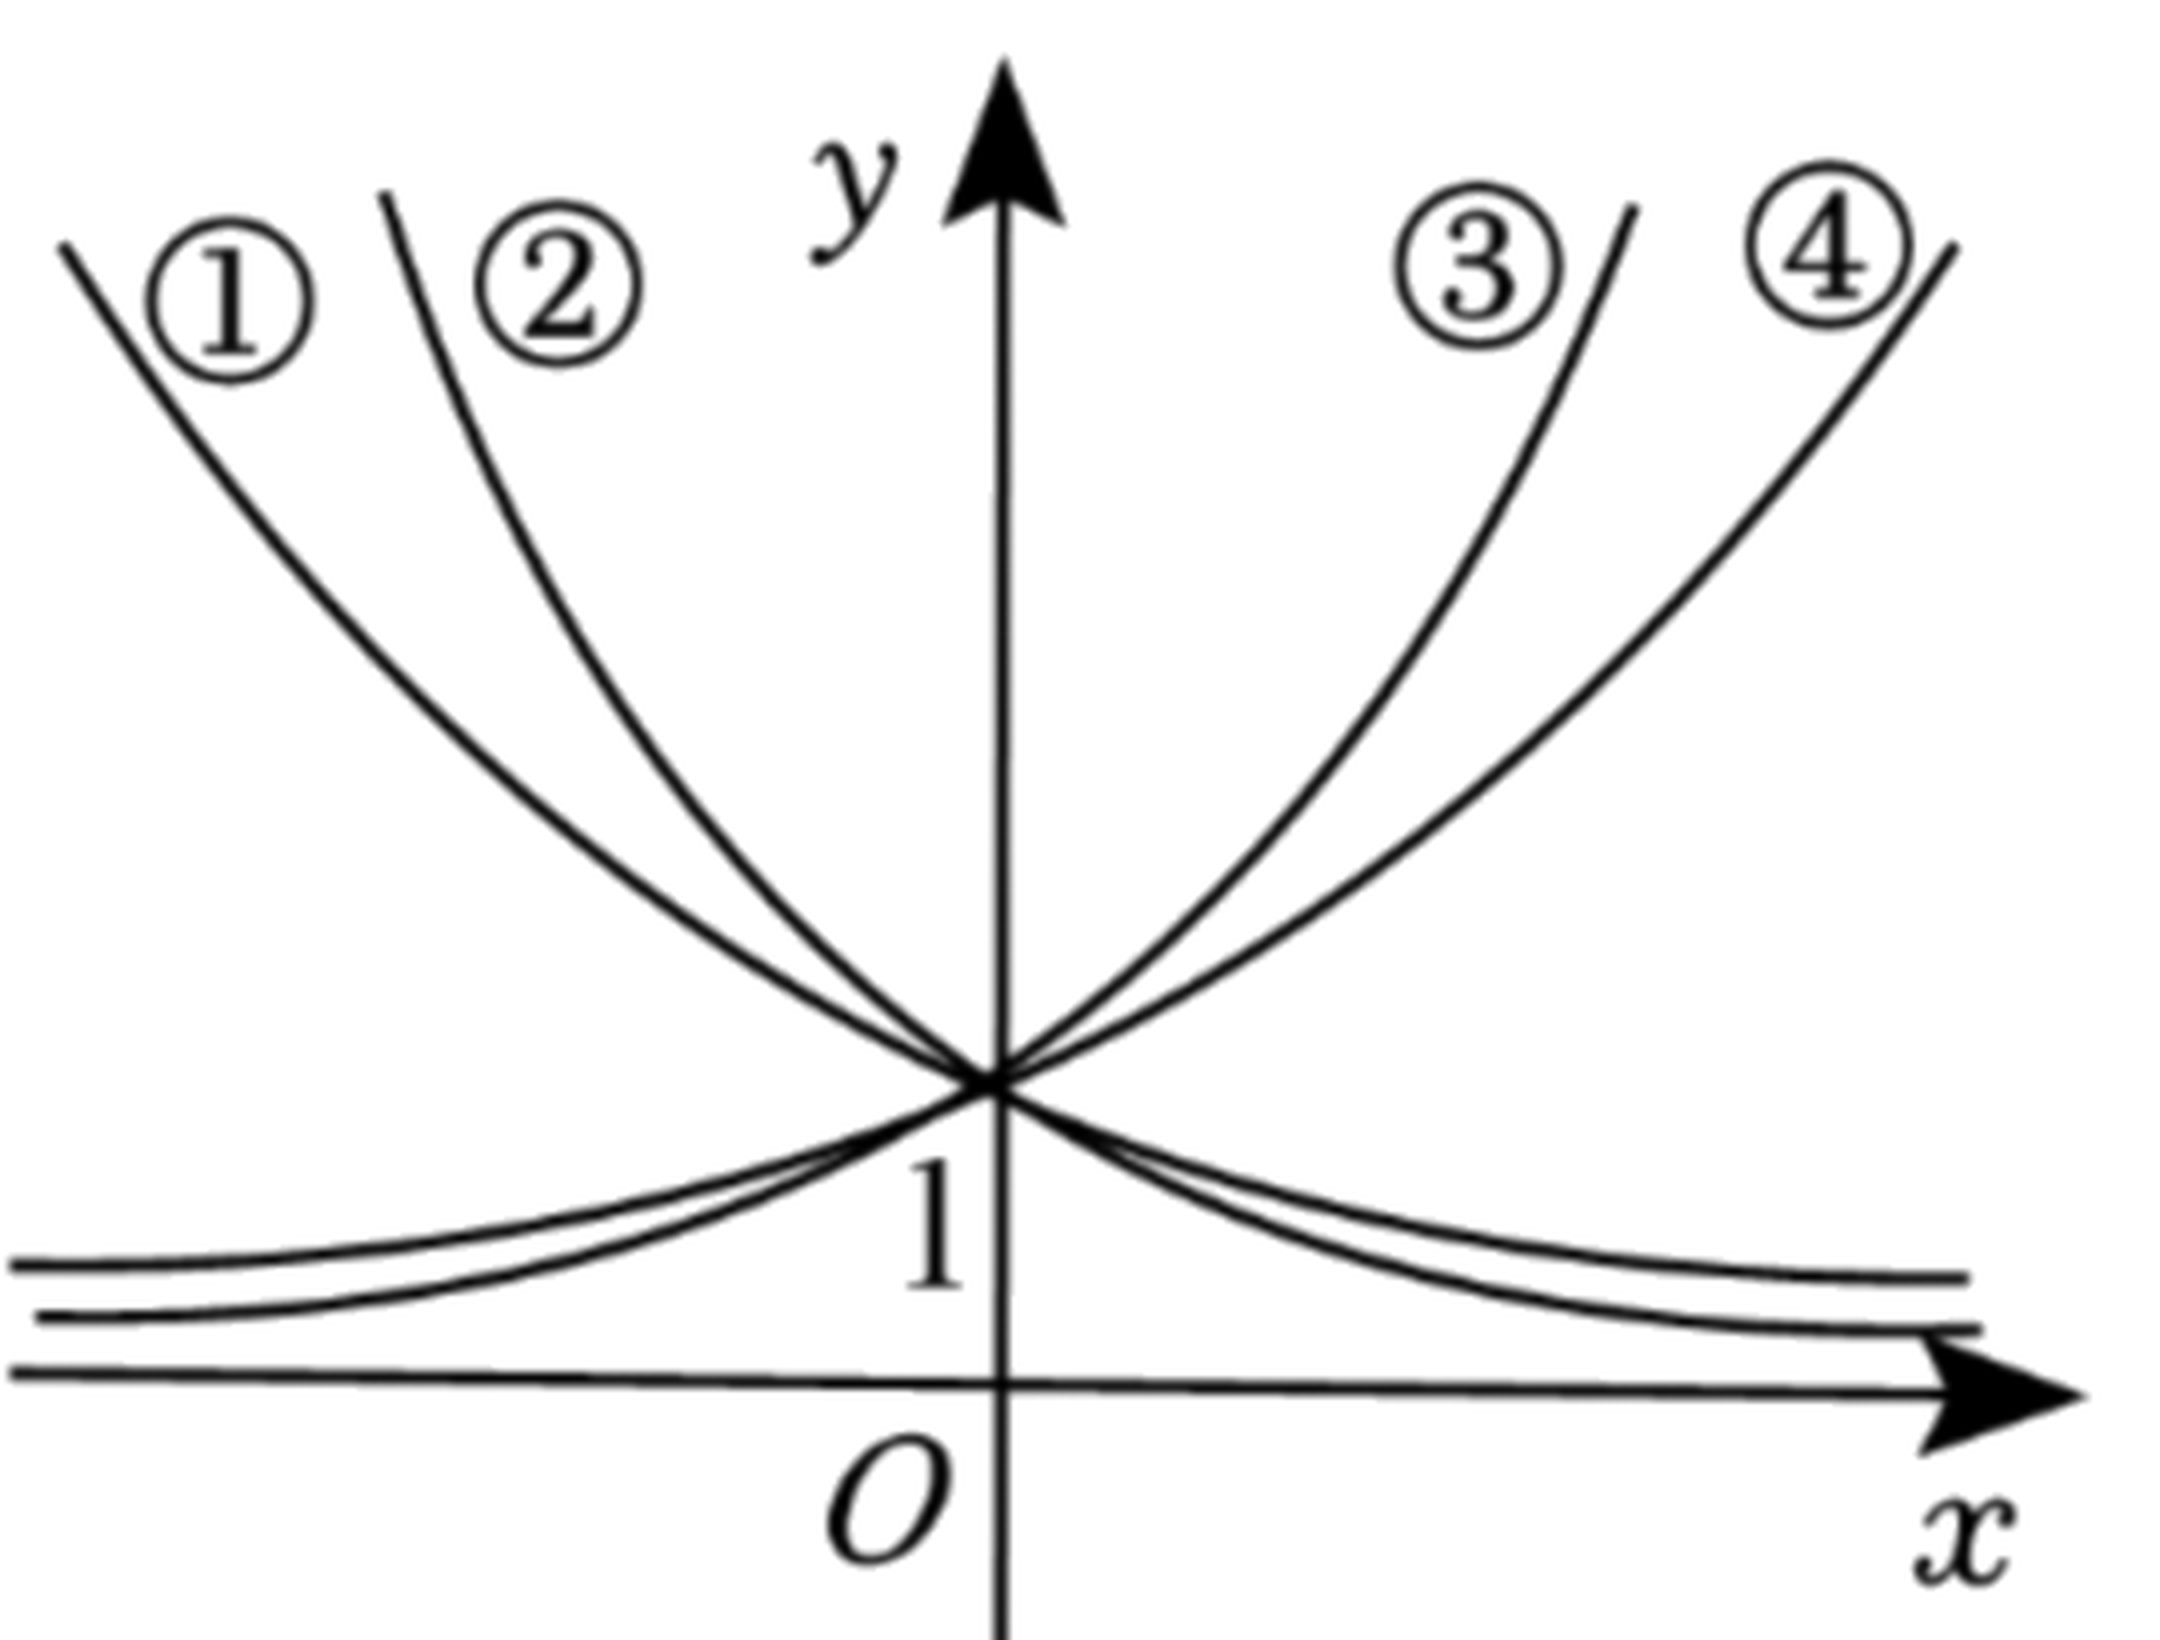
\includegraphics[width=0.40\textwidth]{figures/gao148_q15.png}
\end{center}

\ifanswer
\solbegin
\step{由函数图象得函数① $y=a^x$；② $y=b^x$ 为减函数，且 $x=1$ 时，$b^1<a^1$，}
\step{所以 $0<b<a<1$，}
\step{由函数图象得函数③ $y=c^x$；④ $y=d^x$ 为增函数，且 $x=1$ 时，$c^1>d^1$，}
\step{所以 $c>d>1$，}
\step{所以 $b<a<d<c$. 故选 $B$.}
\solend
\fi

% === Q16 ===：题目配图（关于 y 轴对称的幂函数曲线，三版都出），\needvspace 守卫放 \item 之前；$p$、$q\in\Z$；"图象"照录；解析 2 行
\needvspace{8cm}
\item 已知幂函数 $y=x^{\frac{p}{q}}$（$p$、$q\in\Z$ 且 $p$、$q$ 互质）的图象关于 $y$ 轴对称，如图所示，则\mbox{（\quad）}

\keepwithprev
A. $p$、$q$ 均为奇数，且 $\dfrac{p}{q}>0$\qquad\qquad B. $q$ 为偶数，$p$ 为奇数，且 $\dfrac{p}{q}<0$

C. $q$ 为奇数，$p$ 为偶数，且 $\dfrac{p}{q}>0$\qquad\qquad D. $q$ 为奇数，$p$ 为偶数，且 $\dfrac{p}{q}<0$

\begin{center}
% 关于 y 轴对称的幂函数曲线图取 04 页右下，去粉色水印、去色、4× LANCZOS 放大；三版都出
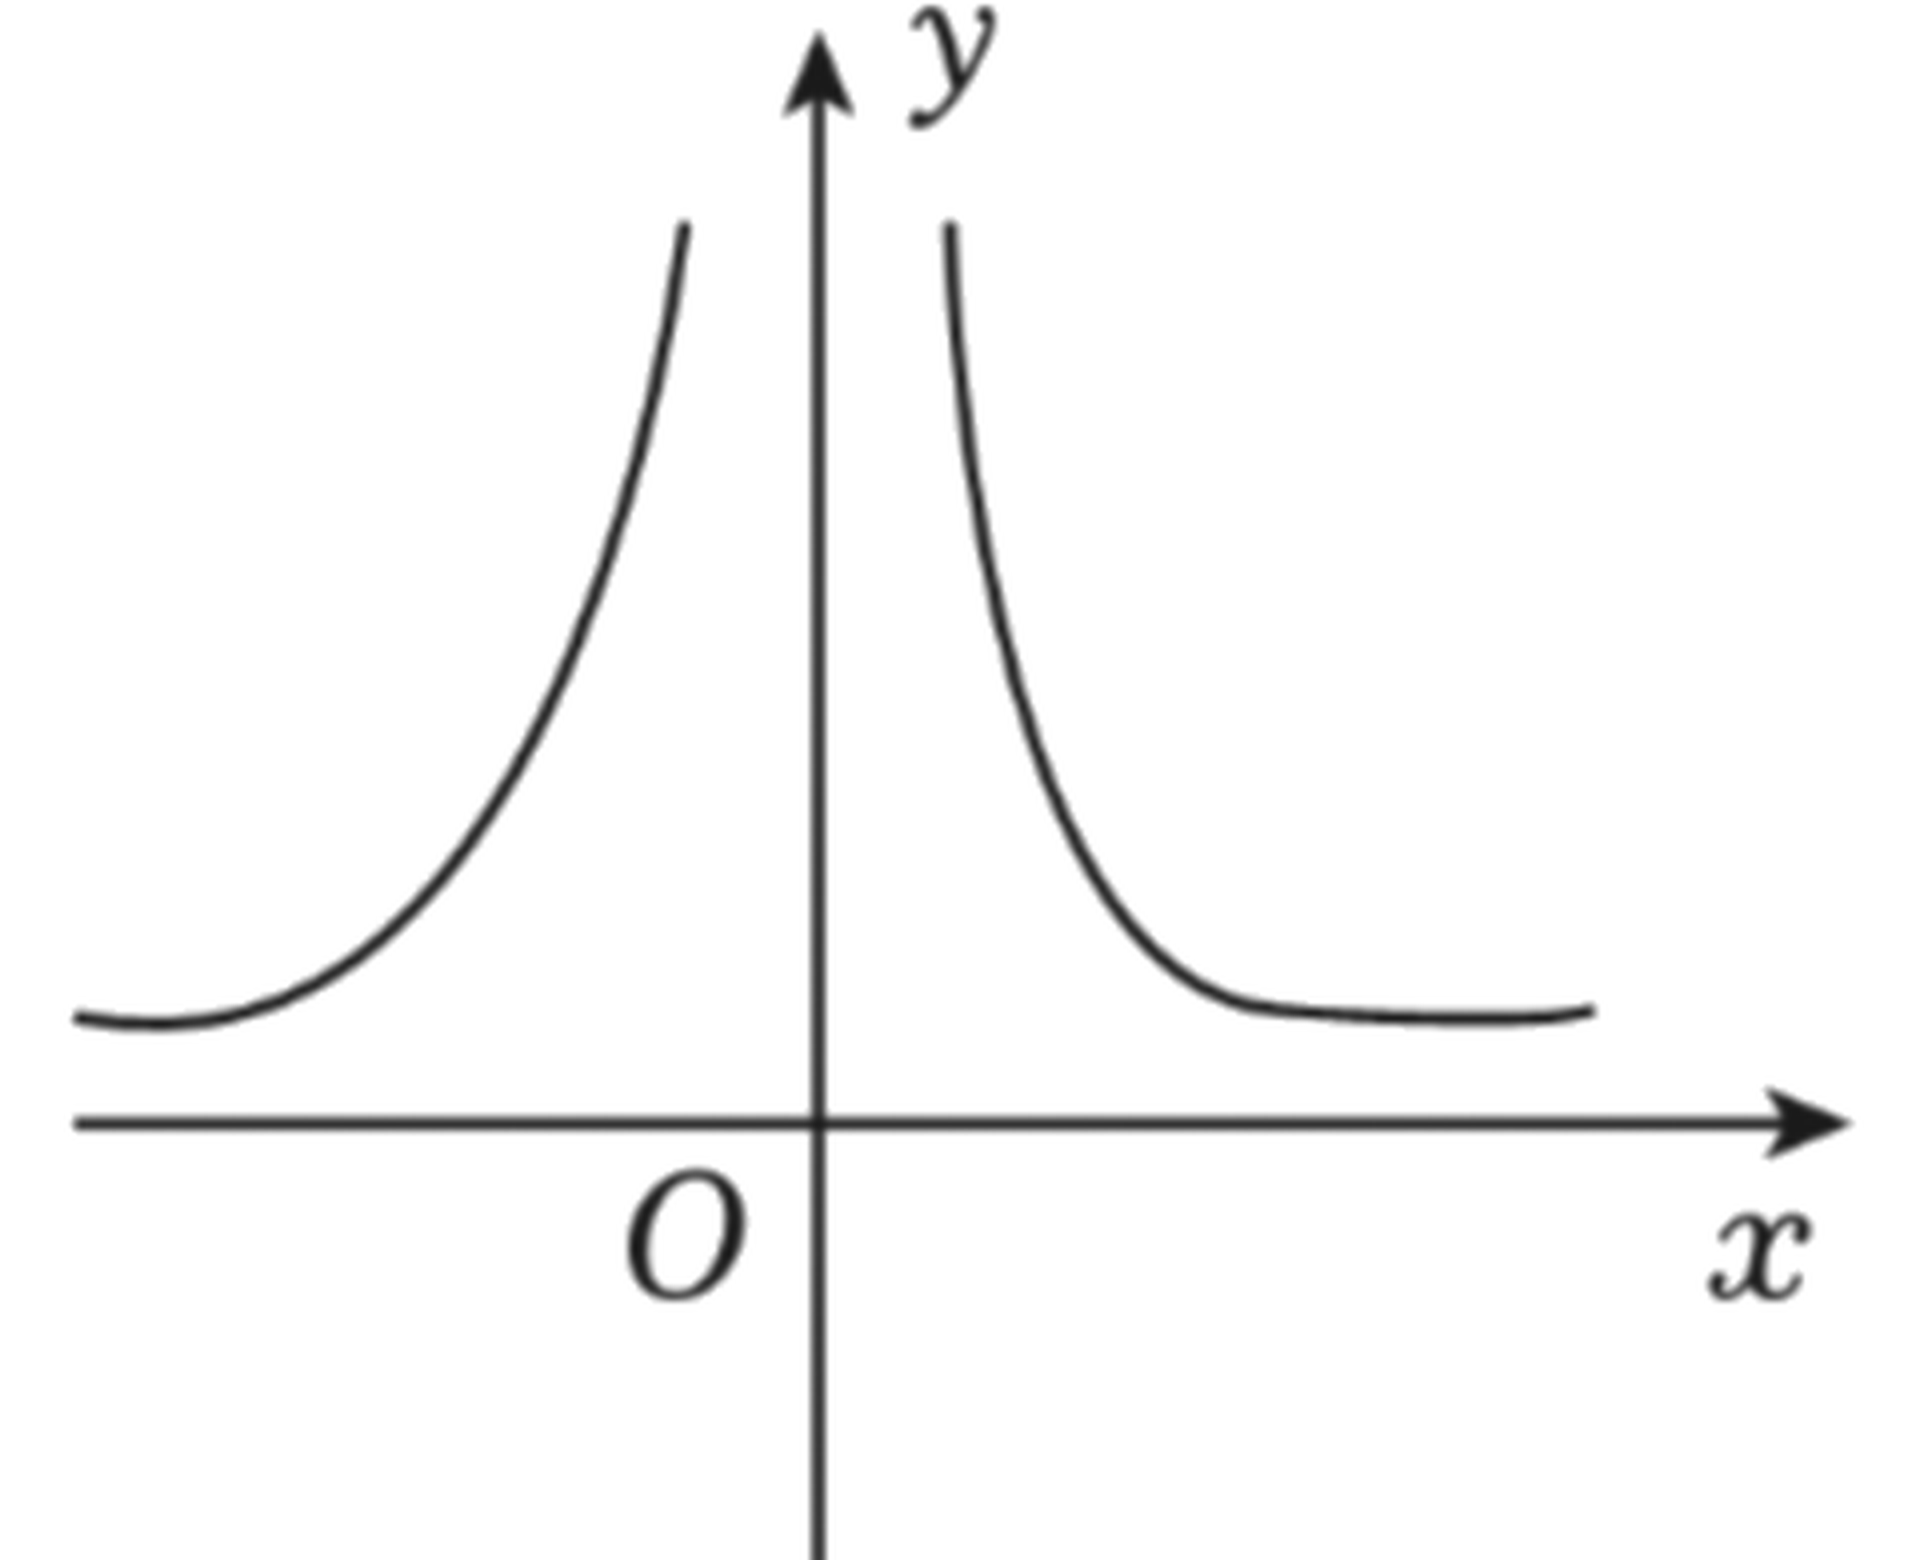
\includegraphics[width=0.36\textwidth]{figures/gao148_q16.png}
\end{center}

\ifanswer
\solbegin
\step{因为函数为偶函数，所以 $p$ 为偶数，且由图象形状判定 $\dfrac{p}{q}<0$.}
\step{又 $p$、$q$ 互质，所以 $q$ 为奇数. 故选 $D$.}
\solend
\fi

\end{enumerate}

\bigsec{三、解答题}

\begin{enumerate}
\setcounter{enumi}{16}

% === Q17 ===：\overline{B}／\varnothing／\R／\mid 逐处照录；解析 8 行
\item 已知集合 $A=\left\{x\mid \dfrac{5}{2x+1}>1\right\}$，$B=\{x\mid x^2+(a+3)x+3a<0,a\in\R\}$.

(1) 求 $A$.

(2) 若全集 $U=\R$，且 $A\cap\overline{B}=\varnothing$，求实数 $a$ 的取值范围.

\ifanswer
\solbegin
\step{(1) $\dfrac{5}{2x+1}>1$，即 $\dfrac{5}{2x+1}-1>0$，即 $\dfrac{4-2x}{2x+1}>0$，即 $(2x+1)(x-2)<0$，}
\step{解得 $-\dfrac{1}{2}<x<2$，所以 $A=\left(-\dfrac{1}{2},2\right)$；}
\step{(2) $x^2+(a+3)x+3a<0$，即 $(x+3)(x+a)<0$，}
\step{全集 $U=\R$，且 $A\cap\overline{B}=\varnothing$，}
\step{当 $a<3$ 时，解得 $-3<x<-a$，则 $\overline{B}=(-\infty,-3)\cup(-a,+\infty)$，}
\step{此时 $-a\geqslant2$，解得 $a\leqslant-2$，}
\step{当 $a\geqslant3$ 时，不满足 $A\cap\overline{B}=\varnothing$，}
\step{故实数 $a$ 的取值范围是 $(-\infty,-2]$.}
\solend
\fi

% === Q18 ===：cases 块整体算一个印刷行；解析 6 行
\item 已知幂函数经过点 $(2,4)$.

(1) 当 $x=\dfrac{1}{2}$ 时，求函数的值；

(2) 是否存在实数 $m$、$n$，使得该函数在区间 $[m,n]$ 上最小值为 $6m-8$，最大值为 $6n-8$？若存在，求出 $m$、$n$ 的值，若不存在，请说明理由.

\ifanswer
\solbegin
\step{(1) 设幂函数的解析式是 $y=x^\alpha$，则 $2^\alpha=4$，解得 $\alpha=2$，}
\step{故 $f(x)=x^2$，$f\left(\dfrac{1}{2}\right)=\dfrac{1}{4}$；}
\step{(2) 因为 $f(x)\geqslant0$，所以 $6m-8\geqslant0$，$m\geqslant\dfrac{4}{3}$，}
\step{由函数 $f(x)$ 在 $(0,+\infty)$ 严格增，得函数 $f(x)$ 在 $(m,n)$ 严格增，}
\step{所以 $\begin{cases}f(m)=6m-8\\f(n)=6n-8\end{cases}$ 且 $m<n$，解得 $m=2$，$n=4$，}
\step{故存在 $m=2$，$n=4$ 满足题意.}
\solend
\fi

% === Q19 ===：7 处评分档照 高一54／64 成例排 \dots\dots N 分；判别式高 \Delta；解析 9 行
\item 已知方程 $x^2+6mx+9m-2=0$，且 $x_1,x_2$ 是方程的两个不同的实数根.

(1) 若 $m=1$，求 $\dfrac{1}{x_1}+\dfrac{1}{x_2}$ 的值；

(2) 若 $m\in\R$，且 $x_1^2+x_2^2<4$，求 $m$ 取值范围.

\ifanswer
\solbegin
\step{(1) 当 $m=1$ 时，方程为 $x^2+6x+7=0$，\dots\dots1 分}
\step{则 $x_1+x_2=-6,x_1\cdot x_2=7$，\dots\dots2 分}
\step{$\dfrac{1}{x_1}+\dfrac{1}{x_2}=\dfrac{x_1+x_2}{x_1\cdot x_2}=-\dfrac{6}{7}$\dots\dots3 分}
\step{(2) $x_1+x_2=-6m,x_1\cdot x_2=9m-2$\dots\dots2 分}
\step{因为 $x_1^2+x_2^2=(x_1+x_2)^2-2x_1\cdot x_2$，所以 $(x_1+x_2)^2-2x_1\cdot x_2<4$，}
\step{所以 $36m^2-2(9m-2)<4$，解得 $0<m<\dfrac{1}{2}$\dots\dots2 分}
\step{又因为方程有两个不同的根，所以 $\Delta=36m^2-4(9m-2)>0$，}% 判别式原卷印等腰偏高粗三角 $\Delta$，照录（放大 07 页 q19_delta3.png／diag_band_q19.png 确认）
\step{解得 $m<\dfrac{1}{3}$ 或 $m>\dfrac{2}{3}$\dots\dots2 分}
\step{所以 $0<m<\dfrac{1}{3}$\dots\dots2 分}
\solend
\fi

% === Q20 ===：题目配图（矩形蔬菜温室，三版都出），\needvspace 守卫放 \item 之前；单位 \mathrm{m}／\mathrm{m}^2；解析 10 行
\needvspace{8cm}
\item 某村计划建造一个室内面积为 $600\mathrm{m}^2$ 的矩形蔬菜温室，在室内，沿左、右两侧与后侧内墙各保留 $2\mathrm{m}$ 宽的通道，沿前侧内墙保留 $4\mathrm{m}$ 宽的空地.

\begin{center}
% 矩形蔬菜温室示意图取 07 页右侧，去粉色水印、去色、4× LANCZOS 放大；三版都出
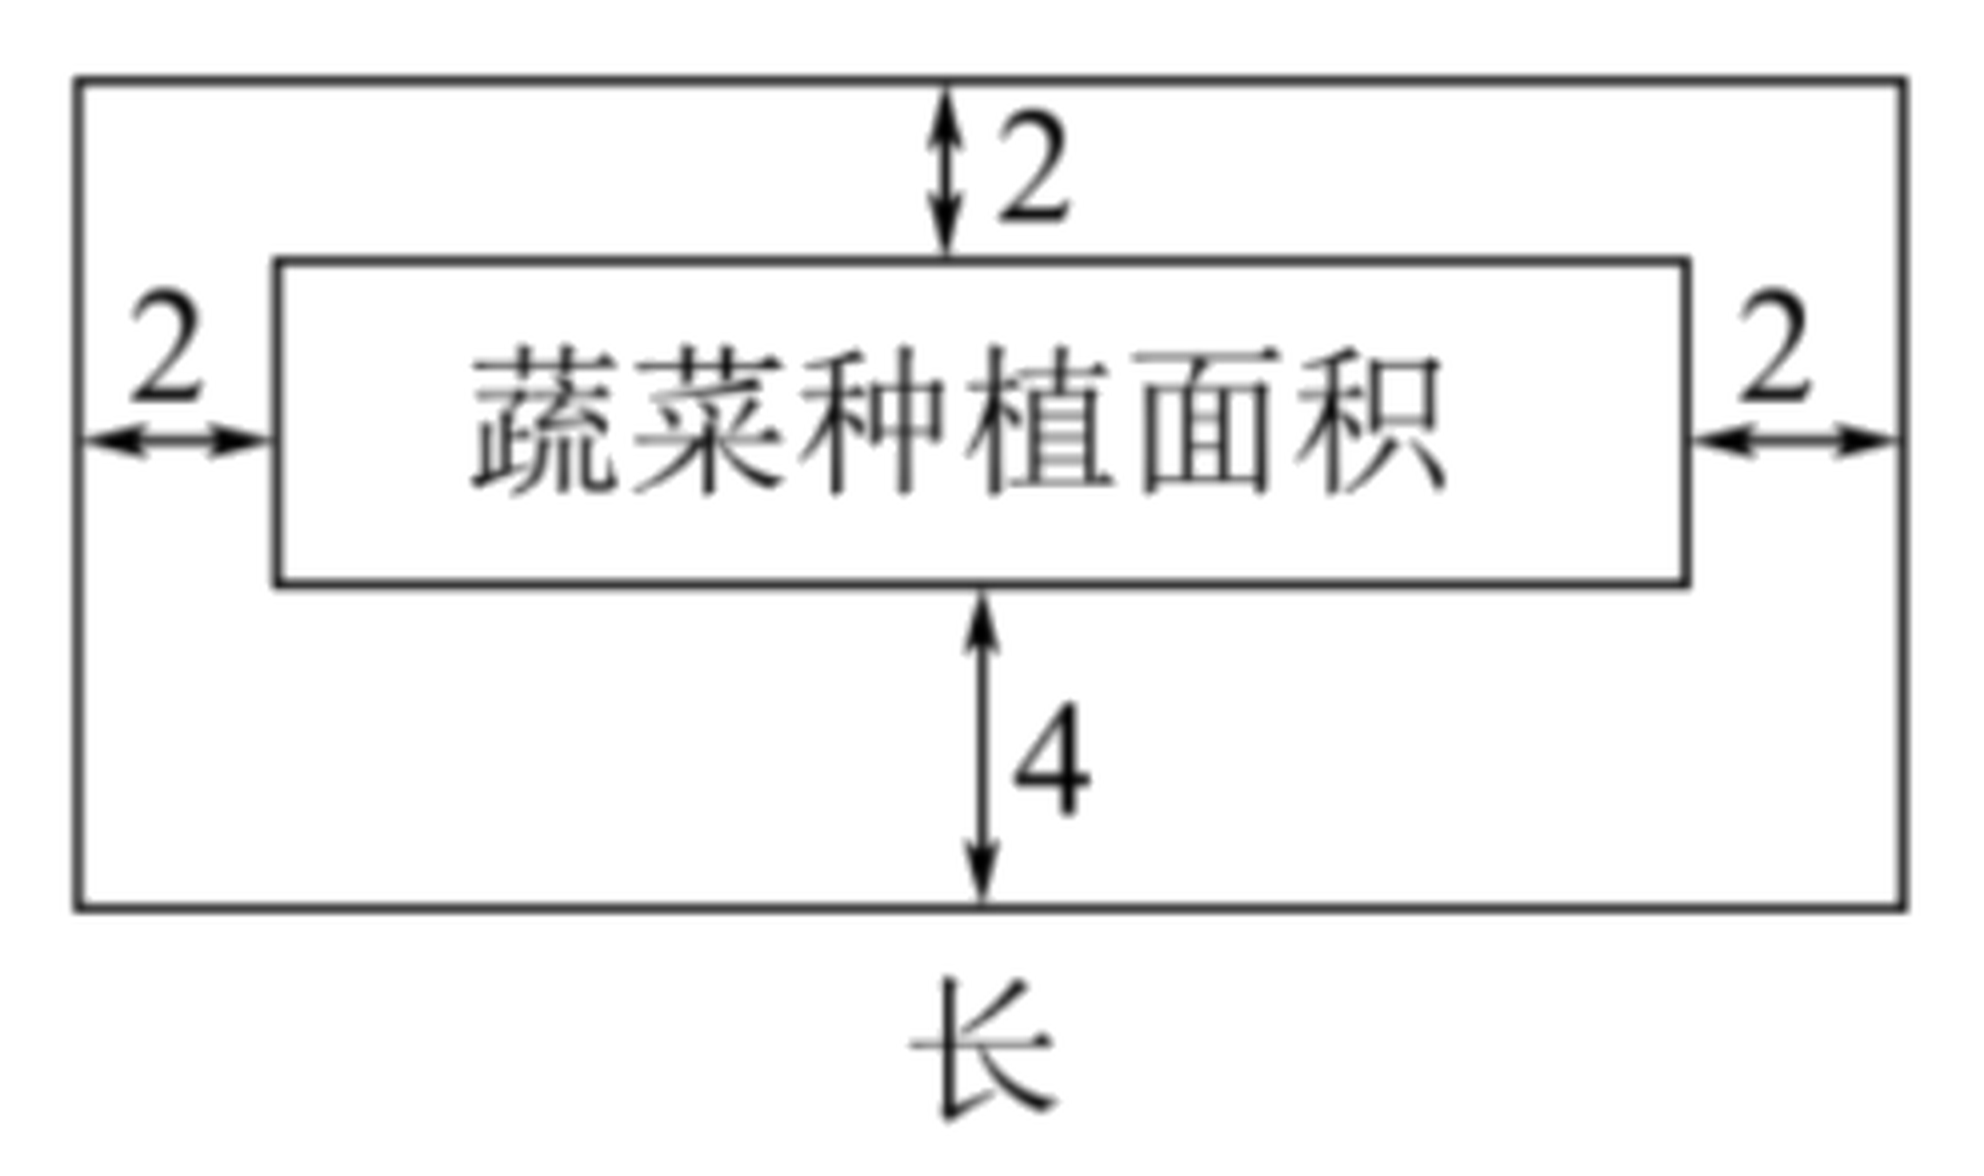
\includegraphics[width=0.45\textwidth]{figures/gao148_q20.png}
\end{center}

(1) 写出蔬菜的种植面积关于矩形温室的长之间的关系式.

(2) 当矩形温室的边长各为多少时，蔬菜的种植面积最大？最大种植面积是多少？

\ifanswer
\solbegin
\step{(1) 设蔬菜的种植面积为 $y\mathrm{m}^2$，矩形温室的长为 $x\mathrm{m}$，}
\step{则矩形温室的宽为 $\dfrac{600}{x}\mathrm{m}$，}
\step{种植蔬菜矩形的长为 $(x-4)\mathrm{m}$，宽为 $\left(\dfrac{600}{x}-6\right)\mathrm{m}$，}
\step{所以 $y=(x-4)\left(\dfrac{600}{x}-6\right)(4<x<100)$；}
\step{(2) 因为 $y=(x-4)\left(\dfrac{600}{x}-6\right)=624-\left(6x+\dfrac{2400}{x}\right)$，}
\step{因为 $6x+\dfrac{2400}{x}\geqslant2\sqrt{6x\cdot\dfrac{2400}{x}}=240$，}
\step{当且仅当 $6x=\dfrac{2400}{x}$，即 $x=20$ 时取等号，}
\step{所以 $y=624-\left(6x+\dfrac{2400}{x}\right)\leqslant624-240=384$.}
\step{即当矩形温室的一边长为 $20\mathrm{m}$，另一边长为 $30\mathrm{m}$ 时，}
\step{蔬菜的种植面积最大，最大为 $384\mathrm{m}^2$.}
\solend
\fi

% === Q21 ===：3 问、cases 块整体算一个印刷行；判别式高 \Delta；解析 19 行（末行续 09 页）
\item 二次函数 $f(x)=ax^2+bx+c$ 满足对任意的 $x\in\R$，$x-1\leqslant f(x)\leqslant x^2-x$ 恒成立.

(1) 求证：$f(1)$ 为定值；

(2) 若 $f(0)=-\dfrac{1}{4}$，求二次函数 $f(x)$ 的表达式；

(3) 求 $a+2b+5c$ 的取值范围.

\ifanswer
\solbegin
\step{(1) 对任意的 $x\in\R$，$x-1\leqslant f(x)\leqslant x^2-x$ 恒成立，则 $0\leqslant f(1)\leqslant0$，}
\step{所以 $f(1)=0$，为定值.}
\step{(2) 由(1)得 $a+b+c=f(1)=0$，由 $f(0)=-\dfrac{1}{4}$，得 $c=-\dfrac{1}{4}$，}
\step{则 $b=\dfrac{1}{4}-a$，$f(x)=ax^2+\left(\dfrac{1}{4}-a\right)x-\dfrac{1}{4}$，}
\step{不等式 $x-1\leqslant f(x)$ 可化为 $ax^2+\left(\dfrac{1}{4}-a\right)x-\dfrac{1}{4}\geqslant x-1$，}
\step{即 $ax^2-\left(a+\dfrac{3}{4}\right)x+\dfrac{3}{4}\geqslant0$，}
\step{一元二次不等式 $ax^2-\left(\dfrac{3}{4}+a\right)x+\dfrac{3}{4}\geqslant0$ 恒成立，则 $\begin{cases}a>0\\\Delta=\left(a+\dfrac{3}{4}\right)^2-3a\leqslant0\end{cases}$，}% 判别式原卷印等腰偏高粗三角 $\Delta$，照录（放大 08 页 q21_delta3.png／diag_band_q21.png 确认）
\step{解得 $a=\dfrac{3}{4}$，}
\step{此时 $f(x)=\dfrac{3}{4}x^2-\dfrac{1}{2}x-\dfrac{1}{4}$，$x^2-x-f(x)=\dfrac{1}{4}(x-1)^2\geqslant0$ 恒成立，}
\step{所以 $f(x)=\dfrac{3}{4}x^2-\dfrac{1}{2}x-\dfrac{1}{4}$.}
\step{(3) 由(1)得 $b=-a-c$，$f(x)=ax^2-(a+c)x+c=(ax-c)(x-1)$，}
\step{不等式 $x-1\leqslant f(x)$ 可化为 $(x-1)(ax-c-1)\geqslant0$，}
\step{一元二次不等式 $(x-1)(ax-c-1)\geqslant0$ 恒成立，则 $a>0$，}
\step{且方程 $(x-1)(ax-c-1)=0$ 有相等的实数根，因此 $c=a-1$，$a>0$，}
\step{不等式 $f(x)\leqslant x^2-x\Leftrightarrow(ax-c)(x-1)\leqslant x^2-x\Leftrightarrow(x-1)[(1-a)x+c]\geqslant0$，}
\step{同理 $1-a>0$，且方程 $(x-1)[(1-a)x+c]=0$ 有相等的实数根，}
\step{因此 $c=a-1$，$a<1$，从而 $c=a-1$，$b=1-2a$，$0<a<1$，}
\step{$a+2b+5c=a+2(1-2a)+5(a-1)=2a-3\in(-3,-1)$，}
\step{所以 $a+2b+5c$ 的取值范围是 $(-3,-1)$.}
\solend
\fi

\end{enumerate}

\end{document}
"
% 紧凑版：xelatex "\def\iscompact{1}% 高一148_新川中学_期中.tex
%   —— 高一上数学"2026-2027 年新川中学高一上期中"（试卷版/答案版/紧凑版）
% 试卷版：xelatex 高一148_新川中学_期中.tex
% 答案版：xelatex "\def\isanswer{1}\input{高一148_新川中学_期中.tex}"
% 紧凑版：xelatex "\def\iscompact{1}\input{高一148_新川中学_期中.tex}"
%
% ① 原始材料：微信公众号"魔都数学加油站"文章，连载"27学年高一148"，原文标题
% "27学年高一148——2026-2027年上海市新川中学高一上期中"（2026-11-21 推送）；
% 原文链接：https://mp.weixin.qq.com/s/Alhmwb3sSLQMp_wjzoAVyA 。
% 正文为 9 张 PNG 页（01/03/04/07/08/09 为 2560×3620，02/05/06 为 4762×6735，
% 同一篇各页分辨率混排，逐页按各自分辨率裁图核对，别按预览比例换算裁框）。
% 体例：混合体例讲评版——19 题中 Q4、Q5 只印【答案】、无【解析】；Q13 的答案"C"
% 直接印在题干括号内、无【答案】/【解析】段；其余 16 题印【解析】（逐题核实，见 ② ②）。
% 题目、答案、解析均据原图转录；卷面粉红色水印"魔都数学加油站"及公众号页脚未录入。
% 全卷插图清单（逐页通读 9 页确认）：4 幅题目配图，均三版都出、均非【解析】内配图：
%   · Q12 幂函数曲线族图（03 页右侧：x/y 轴、O、A(1,0)、B(0,1)、M、N 与两族
%     y=x^α／y=x^β 曲线、线段 AB、虚线），题干"（如图）"处，裁 figures/gao148_q12.png；
%   · Q15 四条指数函数曲线图（04 页右侧：①②③④ 四曲线同过 (0,1)、x/y 轴、O、
%     y 轴刻度 1），题干"如图"处，裁 figures/gao148_q15.png；
%   · Q16 关于 y 轴对称的幂函数曲线图（04 页右下：x/y 轴、O、两支上翘曲线），
%     题干"如图所示"处，裁 figures/gao148_q16.png；
%   · Q20 矩形蔬菜温室示意图（07 页右侧：大矩形＋内框"蔬菜种植面积"＋2/2/4
%     通道标注＋"长"），题干处，裁 figures/gao148_q20.png；
%   其余各页逐页确认无其它题目配图、无【解析】内配图、无表格，亦无"题干写如图而
%   源码漏图"一处；Q19 解析行末的虚线"----N 分"为评分档（非图），Q18／Q21 的
%   cases 块为数学块（非图）。4 图均取自原卷截图，去粉色水印、去色、4× LANCZOS 放大。
%
% 卷首标题：原卷印作"2026-2027 年新川中学高一上期中"，年份区间按全稿惯例排 en dash；
% 原卷卷面未印副标题，本稿按同期中卷（高一140／141／143／144／145／146／147）知识模块
% 口径补出"集合与常用逻辑用语、不等式、函数"。
%
% 题号体例（逐页核实定稿）：本卷共 19 题——一、填空题 3—12（10 题）、
% 二、选择题 13—16（4 题）、三、解答题 17—21（5 题）。
% 三节分别 \setcounter{enumi}{2}／{12}／{16}。原卷从第 3 题起、无第 1、2 题，
% 本稿保留原题号；全卷无附加题节、无 Q22（Q21 解析末行"所以 a+2b+5c 的取值范围是
% (-3,-1)."为全卷收尾，09 页下半仅水印、无正文）。
%
% ② 与原卷的排版差异：
%   ① 原文从第 3 题起，本稿保留原题号；共 19 题三节；
%   ② 混合体例逐题核实：Q4（反证法"假设的内容"）、Q5 只印【答案】、无【解析】，
%      按 高一140 第 5 题／高一145 Q3 成例提 \ans{}、不补造解析；Q13 答案"C"直接
%      印在题干括号内（" ( C ) "）、全卷无该题【答案】/【解析】段，按 高一84 Q13／
%      高一37 Q13／高一53 Q13 成例括号 \mbox{（\quad）} 留空、另提 \ans{$C$}；
%      其余 16 题印【解析】、用 \solbegin…\solend，选择题答案在解析末句"故选 X"
%      （Q14 选 D、Q15 选 B、Q16 选 D，逐个放大原图核实）、题干括号留空、不另提
%      \ans{}；答案版【答案】/【解析】标记数 = 19（3 个 \ans ＋ 16 个 \solbegin）
%      = 全卷题数；
%   ③ 原卷卷面未印副标题，本稿按知识模块口径补出；
%   ④ 原卷填空横线按全稿惯例排 \blankline[4.4em]；选择题括号排 \mbox{（\quad）}、
%      选项段前按惯例加 \keepwithprev；Q13／Q16 四选项为两行两列、Q14／Q15 选项
%      为一行，照原卷分行；解答题不留作答区、不加 \anspace（原卷为讲评版，
%      与 129／131／132／133／136／140／141／143／144／145／146 同）；
%   ⑤ 数集：Q11"在 R 上定义运算"、Q13"x、y∈R"、Q16"p、q∈Z"、Q17"a∈R"
%      "U=R"、Q19"m∈R"、Q21"x∈R" 原卷印斜体 R/Z，按全稿惯例统一改 \R／\Z
%      （本卷未出现 N，\N^* 无对应处）；绝对值排 \lvert…\rvert（Q9／Q14），
%      集合描述竖线排 \mid（Q17）；不等号按全稿惯例排 \leqslant／\geqslant；
%      补集照原卷上划线排 \overline{B}（Q17 题干 1 处＋解析 3 处）；空集
%      \varnothing（Q17 题干 1 处＋解析 2 处）；\subset（Q3 题干 {a}⊂M）与
%      \subseteq（Q3 题干 M⊆{a,b,c,d}）逐处照录不统一（放大 01 页 q3_subset.png）；
%   ⑥ 子题标号 (1)(2)(3) 半角括号照录；圈数字 ①—⑥ 在文本模式（Q14 六个结论、
%      Q15 曲线编号与其解析、Q14 解析"对①…对⑥"），按 common.sty 划入 CJK 字符类
%      渲染；cases 块整体算一个印刷行；\left…\right 不得拆到不同 $…$ 组；
%      单位 m／m² 排 \mathrm{m}／\mathrm{m}^2（Q20，原卷印正体 m）；
%   ⑦ 题干／解析中的中文弯引号按原卷照录：Q4" ab 可以被 5 整除，那么 a、b 中
%      至少有一个能被 5 整除 "（开引号后有空格、闭引号后空格接"时"）、
%      Q13" x=0 "" xy=0 "（引号内空格），注释内一律 ASCII 引号；
%   ⑧ 半角逗号在数学组之间是全稿惯例、非笔误（Q3"{a,b,c,d}"、Q6"$x,y$"
%      "$x=\frac13,y=\frac16$"、Q10、Q11"$a=-2,b=-1"、Q12"$\alpha=\log..,\beta=..$"、
%      Q14"$a+b<0,a-b<0$"、Q17、Q19"$x_1+x_2=-6,x_1\cdot x_2=7$"、Q20、Q21 等），
%      逐处照录别改全角；行末西文句点照录为 ASCII `.`；行中全角逗号／顿号照录；
%   ⑨ "图像／图象"逐处放大核：全卷 9 处均印"图象"（象，无亻）、未见"图像"，
%      逐处照录未统一改动（Q8 题干/解析各 1、Q12 题干 2、Q15 题干 1／解析 2、
%      Q16 题干 1／解析 1；放大 02/03/04/05 页 /tmp/gao148/zoom/my_wide_a.png、
%      my_wide_b.png 与宋体参考"象／像"并排确认）；
%   ⑩ 判别式 Δ/△ 混用是照录项：Q11 解析"△=1−4(−a²+a+1)<0"印扁等边空心
%      三角 \triangle；Q19 解析"Δ=36m²−4(9m−2)>0"、Q21 解析 cases 块
%      "Δ=(a+3/4)²−3a≤0" 两处印等腰偏高粗三角 \Delta，逐处放大判断、照录
%      不统一（参照 高一142／144／145 头注④口径，详见 ④）；
%   ⑪ 一条 \step = 原卷解析的一个印刷行，cases 块整体算一个印刷行；别把原卷折行
%      并起来、别把一行拆多条。Q3 六行、Q7 五行（01 页末首行＋02 页顶四行）、
%      Q9 七行、Q11 五行、Q14 八行（对② 的两行公式各占一印刷行）、Q17 八行、
%      Q18 六行、Q19 九行（7 处评分档附在行末）、Q20 十行、Q21 十九行
%      均按印刷行逐条断，不丢行；
%   ⑫ 配图：4 幅均为题目配图（三版都出），放 \item 内题干之后 \begin{center}；
%      大图块加 \needvspace 守卫把整块推走（守卫放 \item 之前，见 高一145 Q14/Q20
%      成例与切页审计 B 类坑）；三版切页审计均"合计异常：无"；
%   ⑬ 跨页续印按题合并：Q3/4/5 在 01 页；Q6 题干＋解析在 01 页；Q7 题干在 01 页
%      末、解析首行在 01 页末续 02 页顶四行；Q8/9/10 在 02 页（Q9 解析续 02 页下半、
%      Q10 题干与解析前 2 行在 02 页末）；Q10 解析末行续 03 页顶；Q11/12 在 03 页、
%      "二、选择题"标题与 Q13/14 题干在 03 页下半；Q13 无解析；Q14 解析在 04 页顶、
%      Q15 题干＋图＋选项＋解析在 04 页、Q16 题干＋图在 04 页末；Q16 选项＋解析＋
%      "三、解答题"标题＋Q17 题干＋解析在 05 页、Q18 题干首句在 05 页末；Q18 题干
%      续＋解析、Q19 题干＋解析前 5 行在 06 页；Q19 解析续 4 行＋Q20 题干＋图＋
%      解析（10 行全部）在 07 页，末行"蔬菜的种植面积最大，最大为 384m²."收尾；
%      Q21 题干＋解析前 18 行在 08 页；Q21 解析末行"所以 a+2b+5c 的取值范围是
%      (-3,-1)."在 09 页上半（09 页下半仅水印、无正文）。本稿按题连排，不丢行、
%      不并折行；
%   ⑭ 原卷解析内无红色"法一／法二"之类小标题，故本卷无 \stepm；水印
%      "魔都数学加油站"红色不录入；Q19 解析 7 处评分档（1/2/3/2/2/2/2 分）
%      原卷在行末印一串虚线，本稿照 高一54／64 成例排 \dots\dots N 分，
%      分值逐处照录、位置不变。
%
% ③ 行数复核：一条 \step／\stepm = 原卷解析的一个印刷行，cases 块作一个印刷行计。
%   逐题数（主会话逐页核对定稿）：Q3：6；Q4：0（只印【答案】、提 \ans{}）；
%   Q5：0（只印【答案】、提 \ans{}）；Q6：2；Q7：5；Q8：2；Q9：7；Q10：3；
%   Q11：5；Q12：2；Q13：0（答案印在题干括号内、另提 \ans{}）；Q14：8；Q15：5；
%   Q16：2；Q17：8；Q18：6；Q19：9；Q20：10；Q21：19。
%   合计 99 条 \step（本卷无 \stepm：解析内无红色"法一／法二"类小标题），
%   与原卷逐题印刷行相等。全卷 16 题设 \solbegin…\solend ＋ 3 处 \ans{}，
%   答案版【答案】/【解析】标记数 = 19 = 全卷题数。
%
% ④ 判别式／子集符号结论（逐处放大原图照录、不得统一，主会话像素级复核）：
%   判别式全卷 3 处，两形混用逐处照录不统一（参照 高一142／144／145 头注④口径）：
%     · Q11 解析"△=1−4(−a²+a+1)<0" 原卷印扁等边空心三角（宽>高、细线），
%       照录 \triangle（放大 03 页 /tmp/gao148/zoom/q11_delta3.png、
%       delta_montage.png 确认）；
%     · Q19 解析"Δ=36m²−4(9m−2)>0" 原卷印等腰偏高粗三角（高>宽），
%       照录 \Delta（放大 07 页 /tmp/gao148/zoom/q19_delta3.png 确认）；
%     · Q21 解析 cases 块"Δ=(a+3/4)²−3a≤0" 原卷印等腰偏高粗三角（高>宽），
%       照录 \Delta（放大 08 页 /tmp/gao148/zoom/q21_delta3.png 确认）。
%   子集／补集：Q3 题干"{a}⊂M⊆{a,b,c,d}" 前者印单线 ⊂、无下划线，照录 \subset；
%     后者印带下划线 ⊆，照录 \subseteq（放大 01 页 /tmp/gao148/zoom/q3_subset.png
%     确认）；Q17 题干 1 处＋解析 3 处共 4 处 \overline{B} 照原卷上划线
%     （B 上横线、非 C_U B）；空集 \varnothing 3 处（Q17 题干 1 处、解析 2 处）；
%     Q17 集合描述竖线 \mid；数集 \R／\Z 归一见 ② ⑤。
%
% ⑤ 存疑照录（放大原图确认，照录未改、正文对应处另有 % 注）：
%   1. Q3 解析末行"所以 M 一共有 3+3+1+1=8 个" 原卷印 $3+3+1+1=8$，按上文
%      四行应为 $1+3+3+1=8$（疑为原卷加数顺序笔误，和仍为 8），放大 01 页
%      /tmp/gao148/zoom/my_q3_sol.png 确认，照录未改。
%   2. Q13 答案"C"直接印在题干括号内、全卷无该题【答案】/【解析】段，按
%      高一84 Q13 成例括号留空、另提 \ans{$C$}（见 ② ②），未补造解析。
%   3. Q19 解析 7 处评分档（"----N 分"）原卷印一串虚线，本稿照 高一54／64
%      成例排 \dots\dots N 分，分值逐处照录、位置不变。
%   4. 判别式 Q11 扁 \triangle 与 Q19／Q21 高 \Delta 两形混用，逐处照录不统一（见 ④）。
%   5. "图像／图象"全卷 9 处均印"图象"、未见"图像"（见 ② ⑨），逐处放大核实照录，
%      未统一改动。
%   全卷除此 5 类外未发现其它笔误／自相矛盾处。
%
% ⑥ 跨页续印按题合并说明：见 ② ⑬。
%
\documentclass[a4paper,11pt]{article}
\usepackage{common}

\begin{document}

\examtitlest[3]{2026--2027 年新川中学高一上期中}{集合与常用逻辑用语、不等式、函数}

\bigsec{一、填空题}

\begin{enumerate}
\setcounter{enumi}{2}

% === Q3 ===：题干 {a}⊂M⊆{a,b,c,d} 两个子集符号逐处照录；解析 6 行
\item 满足 $\{a\}\subset M\subseteq\{a,b,c,d\}$ 的集合 $M$ 有\blankline[4.4em]个.

\ifanswer
\solbegin
\step{$M$ 是 $\{a,b,c,d\}$ 的子集，但必含有元素 $a$，}
\step{当 $M$ 中只一个元素时，$M=\{a\}$ 只有 1 个；}
\step{当 $M$ 中有二个元素时，$M$ 有 3 个；}
\step{当 $M$ 中有三个元素时，$M$ 有 3 个；}
\step{当 $M$ 中有四个元素时，$M$ 有 1 个；}
\step{所以 $M$ 一共有 $3+3+1+1=8$ 个.}% 原卷印 $3+3+1+1=8$（按上文四行应为 $1+3+3+1$），疑为加数顺序笔误，照录未改（放大 01 页 my_q3_sol.png）
\solend
\fi

% === Q4 ===：原卷只印【答案】、无【解析】，按 高一140 第 5 题成例提 \ans{}；弯引号与空格照录
\item 用反证法证明命题 “ $ab$ 可以被 5 整除，那么 $a$、$b$ 中至少有一个能被 5 整除” 时假设的内容应该是\blankline[4.4em].

\ifanswer
\ans{$a$、$b$ 都不能被 5 整除}
\fi

% === Q5 ===：原卷只印【答案】 $[-2,1)$、无【解析】，提 \ans{}
\item 不等式 $\dfrac{x+2}{x-1}\leqslant0$ 的解集为\blankline[4.4em].

\ifanswer
\ans{$[-2,1)$}
\fi

% === Q6 ===：解析 2 行；半角逗号在数学组之间照录
\item 设 $x,y\in(0,+\infty)$，且 $x+4y=1$，则 $\dfrac{1}{x}+\dfrac{1}{y}$ 的最小值为\blankline[4.4em].

\ifanswer
\solbegin
\step{因为 $\dfrac{1}{x}+\dfrac{1}{y}=(x+4y)\left(\dfrac{1}{x}+\dfrac{1}{y}\right)=5+\dfrac{4y}{x}+\dfrac{x}{y}\geqslant5+2\sqrt{\dfrac{4y}{x}\cdot\dfrac{x}{y}}=9$，}
\step{当且仅当 $\dfrac{4y}{x}=\dfrac{x}{y}$，即 $x=2y$，即 $x=\dfrac{1}{3},y=\dfrac{1}{6}$ 时取等号，故最小值为 9.}
\solend
\fi

% === Q7 ===：题干在 01 页末、解析首行在 01 页末续 02 页顶四行；解析 5 行
\item 若不等式 $x^2+ax+b<0$ 的解集为 $(-3,-1)$，则不等式 $bx^2+ax+1\leqslant0$ 的解集为\blankline[4.4em].

\ifanswer
\solbegin
\step{不等式 $x^2+ax+b<0$ 的解集为 $(-3,-1)$，}
\step{所以方程 $x^2+ax+b=0$ 的两个实数根为 $-3$ 和 $-1$，}
\step{由根与系数的关系得 $a=4$，$b=3$，}
\step{故 $bx^2+ax+1\leqslant0$ 可化为 $3x^2+4x+1\leqslant0$，解得 $-1\leqslant x\leqslant-\dfrac{1}{3}$，}
\step{所求不等式 $bx^2+ax+1\leqslant0$ 的解集为 $\left[-1,-\dfrac{1}{3}\right]$.}
\solend
\fi

% === Q8 ===："图象"照录；解析 2 行
\item 函数 $y=a^{x-2}+2(a>0,a\ne1)$ 的图象必经过定点\blankline[4.4em].

\ifanswer
\solbegin
\step{令 $x-2=0$，得 $x=2$，则 $y=a^0+2=3$，}
\step{所以函数 $y=a^{x-2}+2$ 的图象过定点 $(2,3)$.}
\solend
\fi

% === Q9 ===：解析 7 行；首句末西文句点照录
\item 不等式 $\lvert x+3\rvert+\lvert a-x\rvert>6$ 对一切实数 $x$ 恒成立，则实数 $a$ 的取值范围为\blankline[4.4em].

\ifanswer
\solbegin
\step{$\lvert x+3\rvert$ 表示 $x$ 到 $-3$ 的距离，$\lvert a-x\rvert$ 表示 $x$ 到 $a$ 的距离.}
\step{所以它们的和为 $x$ 到 $-3$ 和 $x$ 到 $a$ 的距离之和，}
\step{当 $x$ 位于 $-3$ 和 $a$ 之间时，距离和取得最小值，}
\step{即两点之间的距离 $\lvert a-(-3)\rvert=\lvert a+3\rvert$，}
\step{若最小值 $\lvert a+3\rvert>6$，则原式对所有 $x$ 恒成立.}
\step{解得 $a+3>6$ 或 $a+3<-6$，即 $a>3$ 或 $a<-9$，}
\step{故 $a\in(3,+\infty)$ 或 $a\in(-\infty,-9)$.}
\solend
\fi

% === Q10 ===：题干与解析前 2 行在 02 页末、解析末行续 03 页顶；解析 3 行
\item 已知 $2^a=3$，$\log_3 5=b$，则 $\log_{15}20=$\blankline[4.4em]（用 $a$、$b$ 表示）.

\ifanswer
\solbegin
\step{因为 $2^a=3$，所以 $a=\log_2 3=\dfrac{\lg3}{\lg2}$，又 $\log_3 5=b=\dfrac{\lg5}{\lg3}$，}
\step{所以 $\lg3=a\lg2$，$\lg5=b\lg3=ba\lg2$，}
\step{则 $\log_{15}20=\dfrac{2\lg2+\lg5}{\lg3+\lg5}=\dfrac{2\lg2+ab\lg2}{a\lg2+ab\lg2}=\dfrac{2+ab}{a+ab}$.}
\solend
\fi

% === Q11 ===：在 \R 上定义运算 \otimes；判别式扁 \triangle 照录；解析 5 行
\item 在 $\R$ 上定义运算 $\otimes:x\otimes y=x(1-y)$，若不等式 $(x-a)\otimes(x+a)<1$ 对任意实数 $x$ 恒成立，则 $a$ 的取值范围是\blankline[4.4em].

\ifanswer
\solbegin
\step{由题意得不等式 $(x-a)\otimes(x+a)<1$ 对任意实数 $x$ 恒成立，}
\step{即不等式 $(x-a)(1-x-a)<1$ 对任意实数 $x$ 恒成立，}
\step{即 $x^2-x-a^2+a+1>0$ 对任意实数 $x$ 恒成立，}
\step{所以 $\triangle=1-4(-a^2+a+1)<0$，解得 $-\dfrac{1}{2}<a<\dfrac{3}{2}$，}% 判别式原卷印扁等边空心三角 $\triangle$，照录（放大 03 页 q11_delta3.png 确认）
\step{所以实数 $a$ 的取值范围为 $\left(-\dfrac{1}{2},\dfrac{3}{2}\right)$.}
\solend
\fi

% === Q12 ===：题目配图（幂函数曲线族，三版都出）；"图象"照录；解析 2 行
\needvspace{8cm}
\item 幂函数 $y=x^\alpha$，当 $\alpha$ 取不同的正数时，在区间 $[0,1]$ 上它们的图象是一族美丽的曲线（如图）. 设点 $A(1,0)$，$B(0,1)$，连接 $AB$，线段 $AB$ 恰好被其中的两个幂函数 $y=x^\alpha$，$y=x^\beta$ 的图象三等分，即有 $BM=MN=NA$，那么 $\alpha\beta=$\blankline[4.4em].

\begin{center}
% 幂函数曲线族图取 03 页右侧，去粉色水印、去色、4× LANCZOS 放大；三版都出
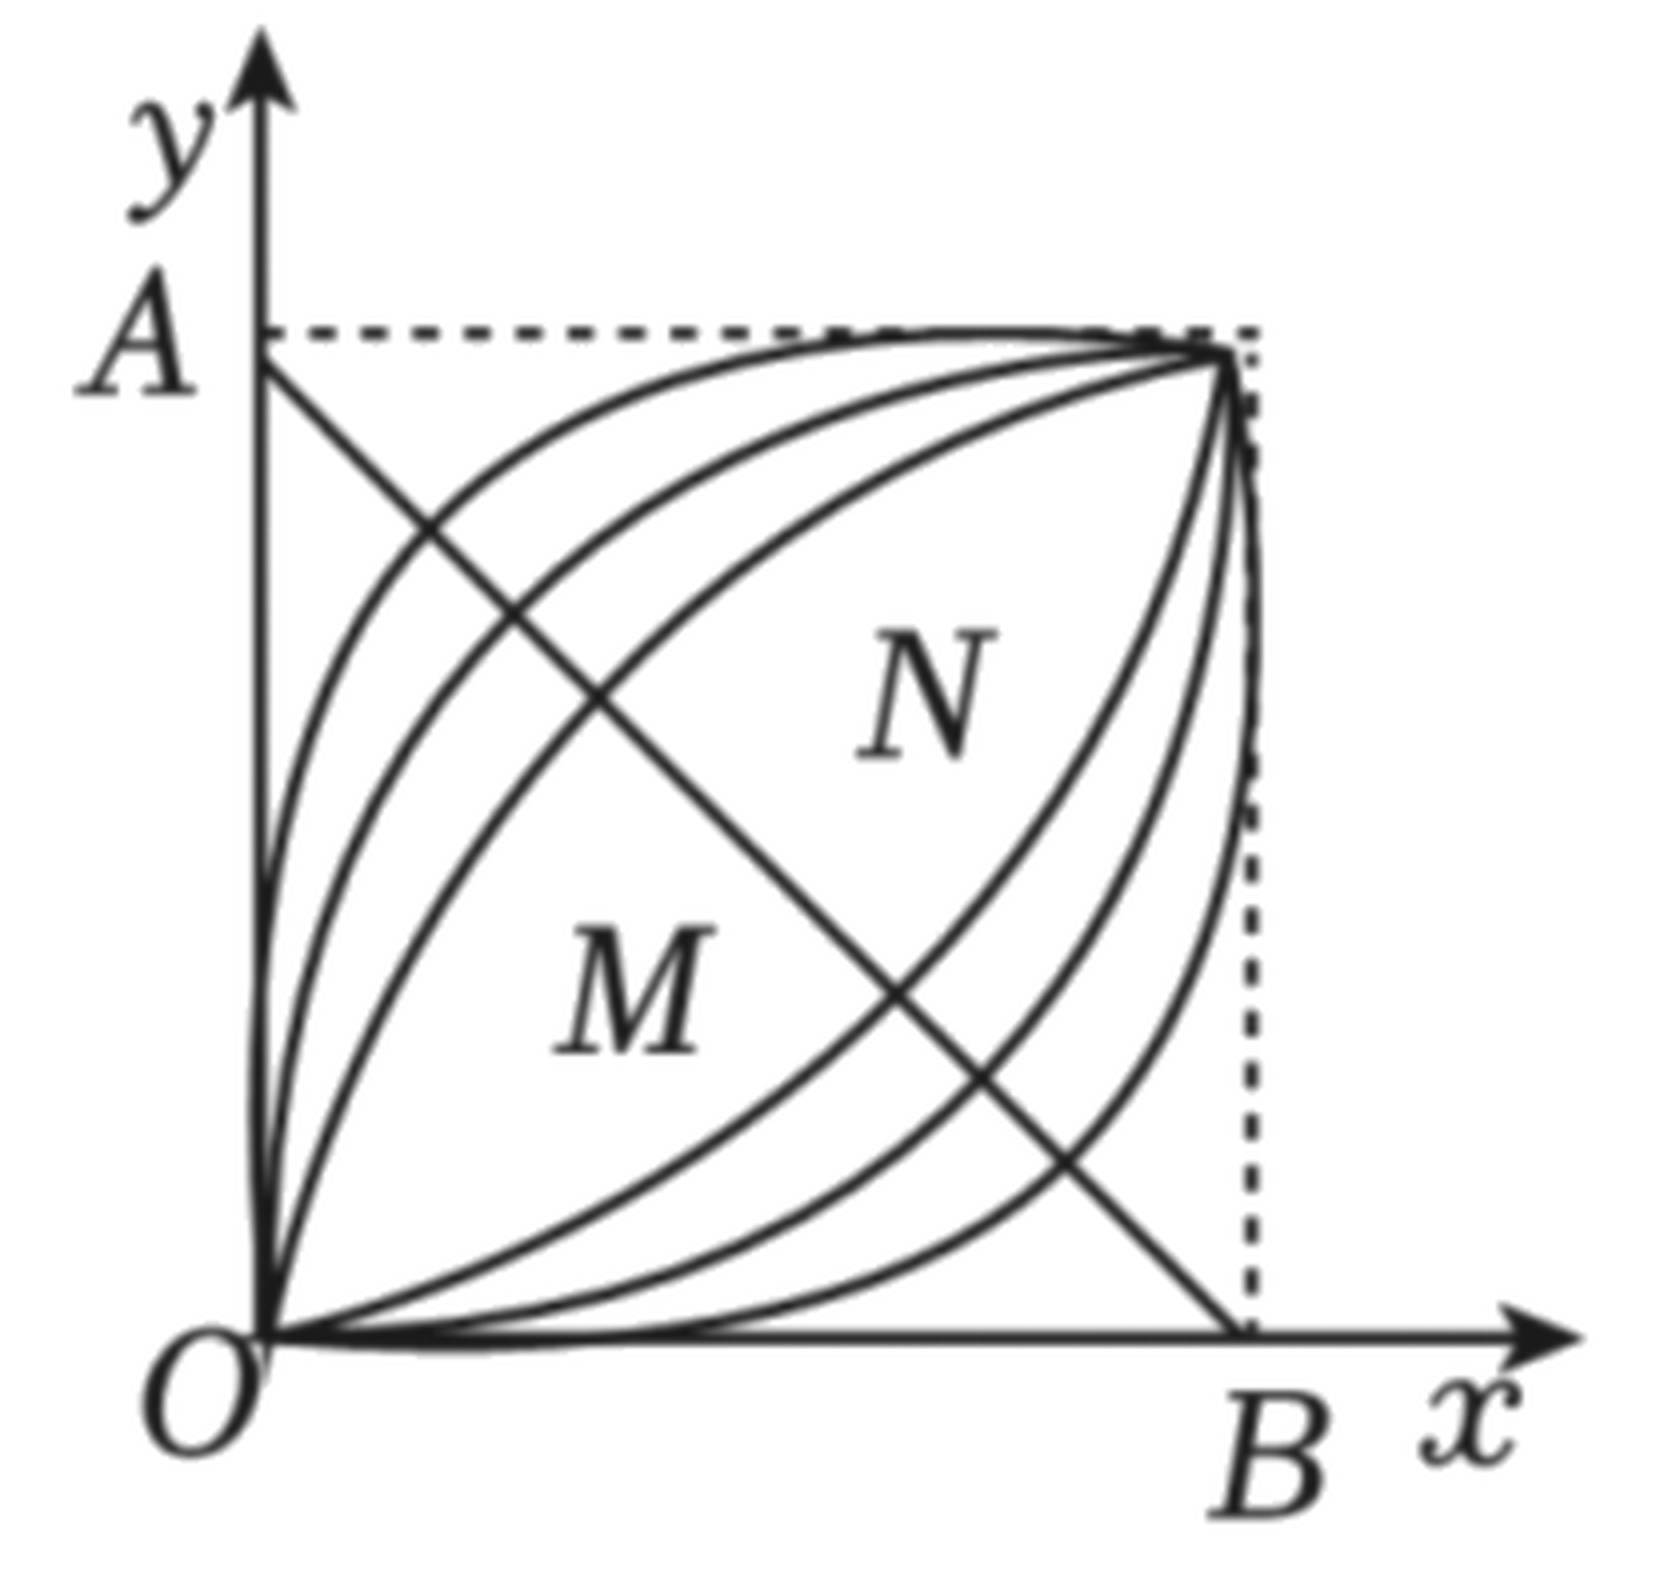
\includegraphics[width=0.40\textwidth]{figures/gao148_q12.png}
\end{center}

\ifanswer
\solbegin
\step{$BM=MN=NA$，点 $A(1,0)$，$B(0,1)$，所以 $M\left(\dfrac{1}{3},\dfrac{2}{3}\right)$，$N\left(\dfrac{2}{3},\dfrac{1}{3}\right)$，}
\step{分别代入 $y=x^\alpha$，$y=x^\beta$，$\alpha=\log_{\frac{2}{3}}\dfrac{1}{3},\beta=\log_{\frac{1}{3}}\dfrac{2}{3}$，$\alpha\beta=\log_{\frac{1}{3}}\dfrac{2}{3}\cdot\log_{\frac{2}{3}}\dfrac{1}{3}=1$.}
\solend
\fi

\end{enumerate}

\bigsec{二、选择题}

\begin{enumerate}
\setcounter{enumi}{12}

% === Q13 ===：答案"C"直接印在题干括号内、全卷无该题【答案】/【解析】段，按 高一84 Q13 成例括号留空、另提 \ans{$C$}；弯引号含空格
\item 若 $x$、$y\in\R$，则 “ $x=0$ ” 是 “ $xy=0$ ” 的\mbox{（\quad）}

\keepwithprev
A. 充要条件\qquad\qquad B. 必要不充分条件

C. 充分不必要条件\qquad\qquad D. 既不充分也不必要条件

\ifanswer
\ans{$C$}
\fi

% === Q14 ===：六个结论（圈数字在文本模式）、四选项一行；解析 8 行（对② 的两行公式各占一印刷行）
\item 若 $a<b<0$，下面有六个结论：① $a^2>b^2$；② $a^3<b^3$；③ $\dfrac{1}{a}<\dfrac{1}{b}$；④ $\dfrac{a}{b}>1$；⑤ $\dfrac{1}{a-b}>\dfrac{1}{a}$；⑥ $\lvert a\rvert>-b$. 其中正确的个数是\mbox{（\quad）}

\keepwithprev
A. 1\qquad\qquad B. 2\qquad\qquad C. 3\qquad\qquad D. 4

\ifanswer
\solbegin
\step{对①：$a^2-b^2=(a+b)(a-b),a+b<0,a-b<0$，故 $a^2-b^2>0$，正确；}
\step{对②：$a^3-b^3=(a-b)(a^2+ab+b^2)=(a-b)\left[\left(a+\dfrac{1}{2}b\right)^2+\dfrac{3}{4}b^2\right],a-b<0$，}
\step{$\left(a+\dfrac{1}{2}b\right)^2+\dfrac{3}{4}b^2>0$，故 $a^3-b^3<0$，正确；}
\step{对③：取 $a=-2,b=-1$，则 $\dfrac{1}{a}=-\dfrac{1}{2},\dfrac{1}{b}=-1,\dfrac{1}{a}>\dfrac{1}{b}$，错误；}
\step{对④：$\dfrac{a}{b}-1=\dfrac{a-b}{b},a-b<0,b<0$，故 $\dfrac{a}{b}-1>0$，正确；}
\step{对⑤：取 $a=-2,b=-1$，则 $\dfrac{1}{a-b}=-1,\dfrac{1}{a}=-\dfrac{1}{2},\dfrac{1}{a-b}<\dfrac{1}{a}$，错误；}
\step{对⑥：要证 $\lvert a\rvert>-b$，即 $-a>-b$，即 $a<b$，正确；}
\step{故选 $D$.}
\solend
\fi

% === Q15 ===：题目配图（四条指数函数曲线，三版都出），\needvspace 守卫放 \item 之前；"图象"照录；解析 5 行
\needvspace{8cm}
\item 如图，曲线①②③④分别是指数函数 $y=a^x$，$y=b^x$，$y=c^x$，$y=d^x$ 的图象，则实数 $a$、$b$、$c$、$d$ 的大小关系为\mbox{（\quad）}

\keepwithprev
A. $a<b<c<d$\qquad B. $b<a<d<c$\qquad C. $d<c<b<a$\qquad D. $c<d<a<b$

\begin{center}
% 四条指数函数曲线图取 04 页右侧，去粉色水印、去色、4× LANCZOS 放大；三版都出
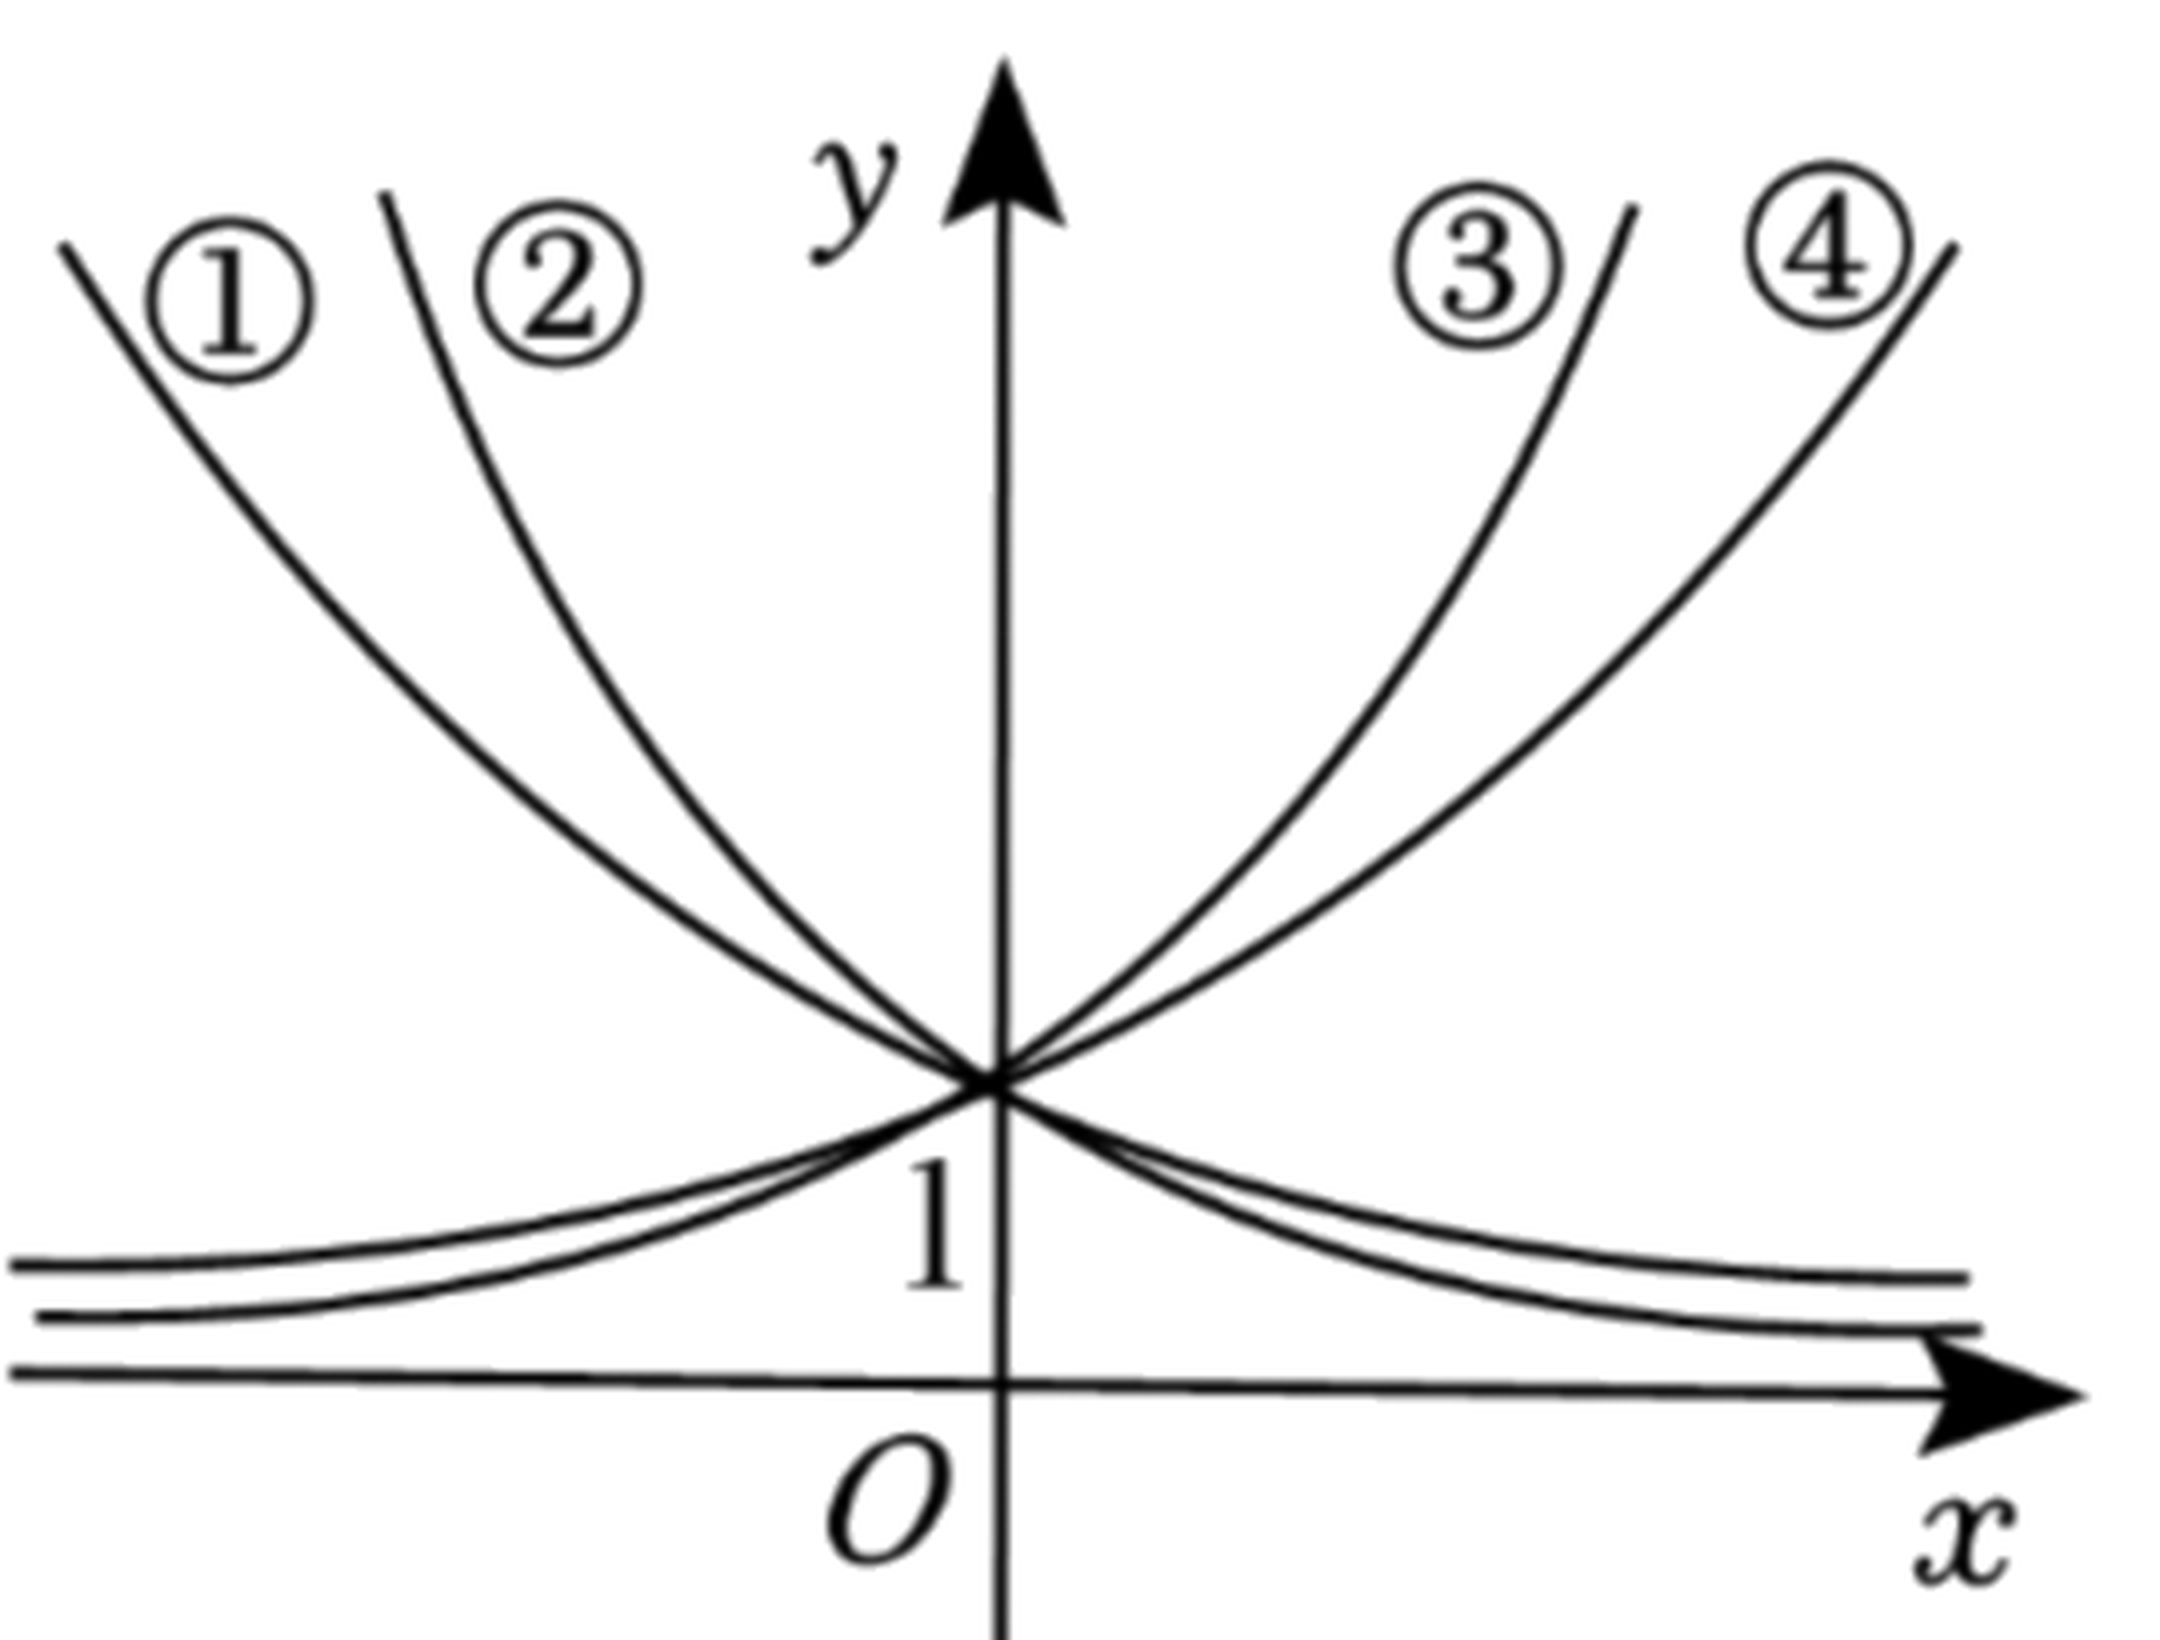
\includegraphics[width=0.40\textwidth]{figures/gao148_q15.png}
\end{center}

\ifanswer
\solbegin
\step{由函数图象得函数① $y=a^x$；② $y=b^x$ 为减函数，且 $x=1$ 时，$b^1<a^1$，}
\step{所以 $0<b<a<1$，}
\step{由函数图象得函数③ $y=c^x$；④ $y=d^x$ 为增函数，且 $x=1$ 时，$c^1>d^1$，}
\step{所以 $c>d>1$，}
\step{所以 $b<a<d<c$. 故选 $B$.}
\solend
\fi

% === Q16 ===：题目配图（关于 y 轴对称的幂函数曲线，三版都出），\needvspace 守卫放 \item 之前；$p$、$q\in\Z$；"图象"照录；解析 2 行
\needvspace{8cm}
\item 已知幂函数 $y=x^{\frac{p}{q}}$（$p$、$q\in\Z$ 且 $p$、$q$ 互质）的图象关于 $y$ 轴对称，如图所示，则\mbox{（\quad）}

\keepwithprev
A. $p$、$q$ 均为奇数，且 $\dfrac{p}{q}>0$\qquad\qquad B. $q$ 为偶数，$p$ 为奇数，且 $\dfrac{p}{q}<0$

C. $q$ 为奇数，$p$ 为偶数，且 $\dfrac{p}{q}>0$\qquad\qquad D. $q$ 为奇数，$p$ 为偶数，且 $\dfrac{p}{q}<0$

\begin{center}
% 关于 y 轴对称的幂函数曲线图取 04 页右下，去粉色水印、去色、4× LANCZOS 放大；三版都出
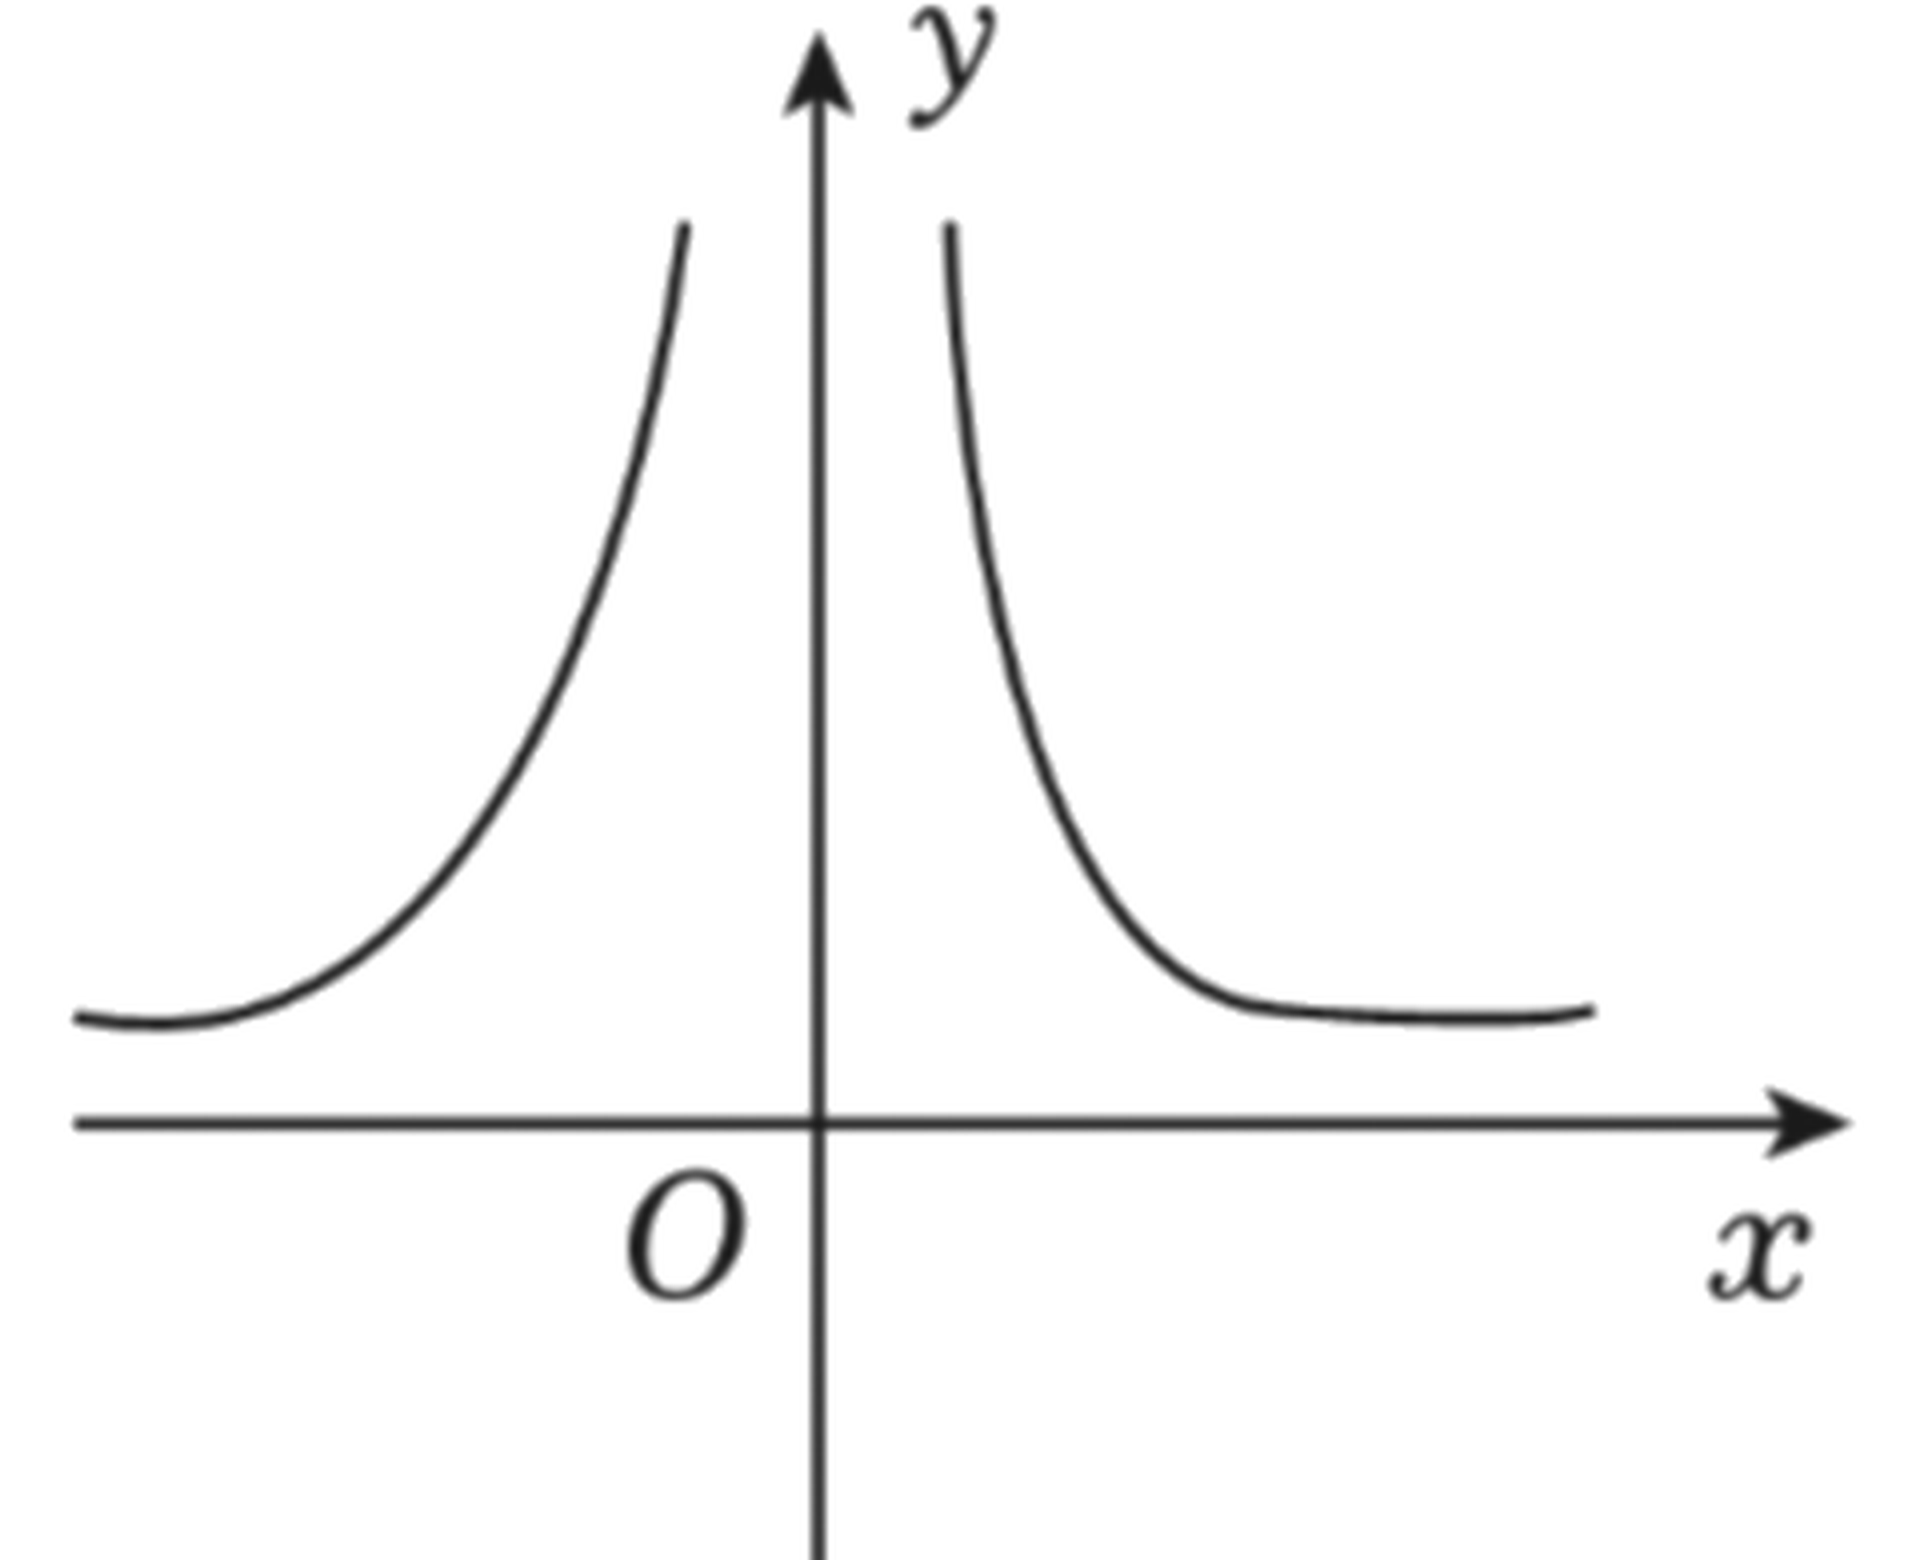
\includegraphics[width=0.36\textwidth]{figures/gao148_q16.png}
\end{center}

\ifanswer
\solbegin
\step{因为函数为偶函数，所以 $p$ 为偶数，且由图象形状判定 $\dfrac{p}{q}<0$.}
\step{又 $p$、$q$ 互质，所以 $q$ 为奇数. 故选 $D$.}
\solend
\fi

\end{enumerate}

\bigsec{三、解答题}

\begin{enumerate}
\setcounter{enumi}{16}

% === Q17 ===：\overline{B}／\varnothing／\R／\mid 逐处照录；解析 8 行
\item 已知集合 $A=\left\{x\mid \dfrac{5}{2x+1}>1\right\}$，$B=\{x\mid x^2+(a+3)x+3a<0,a\in\R\}$.

(1) 求 $A$.

(2) 若全集 $U=\R$，且 $A\cap\overline{B}=\varnothing$，求实数 $a$ 的取值范围.

\ifanswer
\solbegin
\step{(1) $\dfrac{5}{2x+1}>1$，即 $\dfrac{5}{2x+1}-1>0$，即 $\dfrac{4-2x}{2x+1}>0$，即 $(2x+1)(x-2)<0$，}
\step{解得 $-\dfrac{1}{2}<x<2$，所以 $A=\left(-\dfrac{1}{2},2\right)$；}
\step{(2) $x^2+(a+3)x+3a<0$，即 $(x+3)(x+a)<0$，}
\step{全集 $U=\R$，且 $A\cap\overline{B}=\varnothing$，}
\step{当 $a<3$ 时，解得 $-3<x<-a$，则 $\overline{B}=(-\infty,-3)\cup(-a,+\infty)$，}
\step{此时 $-a\geqslant2$，解得 $a\leqslant-2$，}
\step{当 $a\geqslant3$ 时，不满足 $A\cap\overline{B}=\varnothing$，}
\step{故实数 $a$ 的取值范围是 $(-\infty,-2]$.}
\solend
\fi

% === Q18 ===：cases 块整体算一个印刷行；解析 6 行
\item 已知幂函数经过点 $(2,4)$.

(1) 当 $x=\dfrac{1}{2}$ 时，求函数的值；

(2) 是否存在实数 $m$、$n$，使得该函数在区间 $[m,n]$ 上最小值为 $6m-8$，最大值为 $6n-8$？若存在，求出 $m$、$n$ 的值，若不存在，请说明理由.

\ifanswer
\solbegin
\step{(1) 设幂函数的解析式是 $y=x^\alpha$，则 $2^\alpha=4$，解得 $\alpha=2$，}
\step{故 $f(x)=x^2$，$f\left(\dfrac{1}{2}\right)=\dfrac{1}{4}$；}
\step{(2) 因为 $f(x)\geqslant0$，所以 $6m-8\geqslant0$，$m\geqslant\dfrac{4}{3}$，}
\step{由函数 $f(x)$ 在 $(0,+\infty)$ 严格增，得函数 $f(x)$ 在 $(m,n)$ 严格增，}
\step{所以 $\begin{cases}f(m)=6m-8\\f(n)=6n-8\end{cases}$ 且 $m<n$，解得 $m=2$，$n=4$，}
\step{故存在 $m=2$，$n=4$ 满足题意.}
\solend
\fi

% === Q19 ===：7 处评分档照 高一54／64 成例排 \dots\dots N 分；判别式高 \Delta；解析 9 行
\item 已知方程 $x^2+6mx+9m-2=0$，且 $x_1,x_2$ 是方程的两个不同的实数根.

(1) 若 $m=1$，求 $\dfrac{1}{x_1}+\dfrac{1}{x_2}$ 的值；

(2) 若 $m\in\R$，且 $x_1^2+x_2^2<4$，求 $m$ 取值范围.

\ifanswer
\solbegin
\step{(1) 当 $m=1$ 时，方程为 $x^2+6x+7=0$，\dots\dots1 分}
\step{则 $x_1+x_2=-6,x_1\cdot x_2=7$，\dots\dots2 分}
\step{$\dfrac{1}{x_1}+\dfrac{1}{x_2}=\dfrac{x_1+x_2}{x_1\cdot x_2}=-\dfrac{6}{7}$\dots\dots3 分}
\step{(2) $x_1+x_2=-6m,x_1\cdot x_2=9m-2$\dots\dots2 分}
\step{因为 $x_1^2+x_2^2=(x_1+x_2)^2-2x_1\cdot x_2$，所以 $(x_1+x_2)^2-2x_1\cdot x_2<4$，}
\step{所以 $36m^2-2(9m-2)<4$，解得 $0<m<\dfrac{1}{2}$\dots\dots2 分}
\step{又因为方程有两个不同的根，所以 $\Delta=36m^2-4(9m-2)>0$，}% 判别式原卷印等腰偏高粗三角 $\Delta$，照录（放大 07 页 q19_delta3.png／diag_band_q19.png 确认）
\step{解得 $m<\dfrac{1}{3}$ 或 $m>\dfrac{2}{3}$\dots\dots2 分}
\step{所以 $0<m<\dfrac{1}{3}$\dots\dots2 分}
\solend
\fi

% === Q20 ===：题目配图（矩形蔬菜温室，三版都出），\needvspace 守卫放 \item 之前；单位 \mathrm{m}／\mathrm{m}^2；解析 10 行
\needvspace{8cm}
\item 某村计划建造一个室内面积为 $600\mathrm{m}^2$ 的矩形蔬菜温室，在室内，沿左、右两侧与后侧内墙各保留 $2\mathrm{m}$ 宽的通道，沿前侧内墙保留 $4\mathrm{m}$ 宽的空地.

\begin{center}
% 矩形蔬菜温室示意图取 07 页右侧，去粉色水印、去色、4× LANCZOS 放大；三版都出
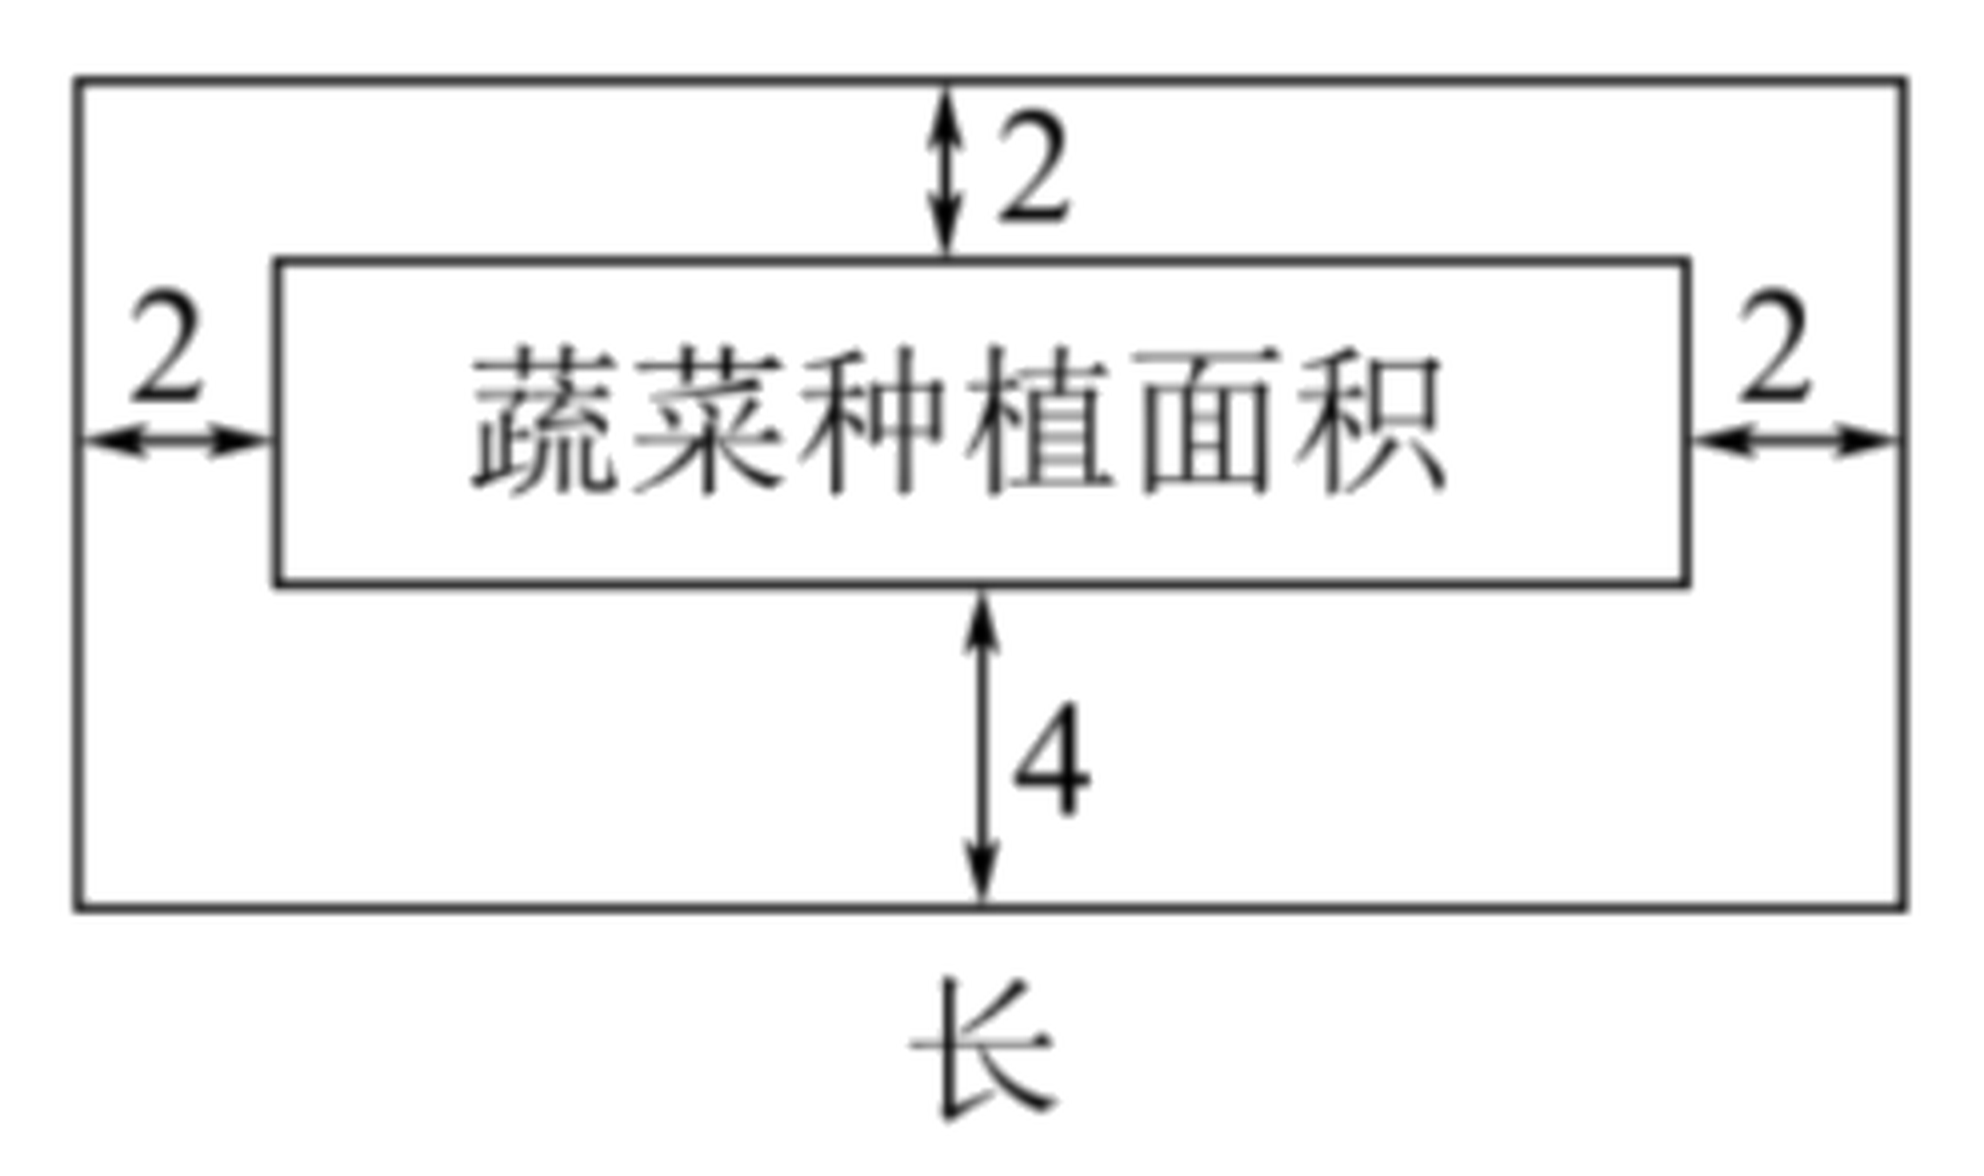
\includegraphics[width=0.45\textwidth]{figures/gao148_q20.png}
\end{center}

(1) 写出蔬菜的种植面积关于矩形温室的长之间的关系式.

(2) 当矩形温室的边长各为多少时，蔬菜的种植面积最大？最大种植面积是多少？

\ifanswer
\solbegin
\step{(1) 设蔬菜的种植面积为 $y\mathrm{m}^2$，矩形温室的长为 $x\mathrm{m}$，}
\step{则矩形温室的宽为 $\dfrac{600}{x}\mathrm{m}$，}
\step{种植蔬菜矩形的长为 $(x-4)\mathrm{m}$，宽为 $\left(\dfrac{600}{x}-6\right)\mathrm{m}$，}
\step{所以 $y=(x-4)\left(\dfrac{600}{x}-6\right)(4<x<100)$；}
\step{(2) 因为 $y=(x-4)\left(\dfrac{600}{x}-6\right)=624-\left(6x+\dfrac{2400}{x}\right)$，}
\step{因为 $6x+\dfrac{2400}{x}\geqslant2\sqrt{6x\cdot\dfrac{2400}{x}}=240$，}
\step{当且仅当 $6x=\dfrac{2400}{x}$，即 $x=20$ 时取等号，}
\step{所以 $y=624-\left(6x+\dfrac{2400}{x}\right)\leqslant624-240=384$.}
\step{即当矩形温室的一边长为 $20\mathrm{m}$，另一边长为 $30\mathrm{m}$ 时，}
\step{蔬菜的种植面积最大，最大为 $384\mathrm{m}^2$.}
\solend
\fi

% === Q21 ===：3 问、cases 块整体算一个印刷行；判别式高 \Delta；解析 19 行（末行续 09 页）
\item 二次函数 $f(x)=ax^2+bx+c$ 满足对任意的 $x\in\R$，$x-1\leqslant f(x)\leqslant x^2-x$ 恒成立.

(1) 求证：$f(1)$ 为定值；

(2) 若 $f(0)=-\dfrac{1}{4}$，求二次函数 $f(x)$ 的表达式；

(3) 求 $a+2b+5c$ 的取值范围.

\ifanswer
\solbegin
\step{(1) 对任意的 $x\in\R$，$x-1\leqslant f(x)\leqslant x^2-x$ 恒成立，则 $0\leqslant f(1)\leqslant0$，}
\step{所以 $f(1)=0$，为定值.}
\step{(2) 由(1)得 $a+b+c=f(1)=0$，由 $f(0)=-\dfrac{1}{4}$，得 $c=-\dfrac{1}{4}$，}
\step{则 $b=\dfrac{1}{4}-a$，$f(x)=ax^2+\left(\dfrac{1}{4}-a\right)x-\dfrac{1}{4}$，}
\step{不等式 $x-1\leqslant f(x)$ 可化为 $ax^2+\left(\dfrac{1}{4}-a\right)x-\dfrac{1}{4}\geqslant x-1$，}
\step{即 $ax^2-\left(a+\dfrac{3}{4}\right)x+\dfrac{3}{4}\geqslant0$，}
\step{一元二次不等式 $ax^2-\left(\dfrac{3}{4}+a\right)x+\dfrac{3}{4}\geqslant0$ 恒成立，则 $\begin{cases}a>0\\\Delta=\left(a+\dfrac{3}{4}\right)^2-3a\leqslant0\end{cases}$，}% 判别式原卷印等腰偏高粗三角 $\Delta$，照录（放大 08 页 q21_delta3.png／diag_band_q21.png 确认）
\step{解得 $a=\dfrac{3}{4}$，}
\step{此时 $f(x)=\dfrac{3}{4}x^2-\dfrac{1}{2}x-\dfrac{1}{4}$，$x^2-x-f(x)=\dfrac{1}{4}(x-1)^2\geqslant0$ 恒成立，}
\step{所以 $f(x)=\dfrac{3}{4}x^2-\dfrac{1}{2}x-\dfrac{1}{4}$.}
\step{(3) 由(1)得 $b=-a-c$，$f(x)=ax^2-(a+c)x+c=(ax-c)(x-1)$，}
\step{不等式 $x-1\leqslant f(x)$ 可化为 $(x-1)(ax-c-1)\geqslant0$，}
\step{一元二次不等式 $(x-1)(ax-c-1)\geqslant0$ 恒成立，则 $a>0$，}
\step{且方程 $(x-1)(ax-c-1)=0$ 有相等的实数根，因此 $c=a-1$，$a>0$，}
\step{不等式 $f(x)\leqslant x^2-x\Leftrightarrow(ax-c)(x-1)\leqslant x^2-x\Leftrightarrow(x-1)[(1-a)x+c]\geqslant0$，}
\step{同理 $1-a>0$，且方程 $(x-1)[(1-a)x+c]=0$ 有相等的实数根，}
\step{因此 $c=a-1$，$a<1$，从而 $c=a-1$，$b=1-2a$，$0<a<1$，}
\step{$a+2b+5c=a+2(1-2a)+5(a-1)=2a-3\in(-3,-1)$，}
\step{所以 $a+2b+5c$ 的取值范围是 $(-3,-1)$.}
\solend
\fi

\end{enumerate}

\end{document}
"
%
% ① 原始材料：微信公众号"魔都数学加油站"文章，连载"27学年高一148"，原文标题
% "27学年高一148——2026-2027年上海市新川中学高一上期中"（2026-11-21 推送）；
% 原文链接：https://mp.weixin.qq.com/s/Alhmwb3sSLQMp_wjzoAVyA 。
% 正文为 9 张 PNG 页（01/03/04/07/08/09 为 2560×3620，02/05/06 为 4762×6735，
% 同一篇各页分辨率混排，逐页按各自分辨率裁图核对，别按预览比例换算裁框）。
% 体例：混合体例讲评版——19 题中 Q4、Q5 只印【答案】、无【解析】；Q13 的答案"C"
% 直接印在题干括号内、无【答案】/【解析】段；其余 16 题印【解析】（逐题核实，见 ② ②）。
% 题目、答案、解析均据原图转录；卷面粉红色水印"魔都数学加油站"及公众号页脚未录入。
% 全卷插图清单（逐页通读 9 页确认）：4 幅题目配图，均三版都出、均非【解析】内配图：
%   · Q12 幂函数曲线族图（03 页右侧：x/y 轴、O、A(1,0)、B(0,1)、M、N 与两族
%     y=x^α／y=x^β 曲线、线段 AB、虚线），题干"（如图）"处，裁 figures/gao148_q12.png；
%   · Q15 四条指数函数曲线图（04 页右侧：①②③④ 四曲线同过 (0,1)、x/y 轴、O、
%     y 轴刻度 1），题干"如图"处，裁 figures/gao148_q15.png；
%   · Q16 关于 y 轴对称的幂函数曲线图（04 页右下：x/y 轴、O、两支上翘曲线），
%     题干"如图所示"处，裁 figures/gao148_q16.png；
%   · Q20 矩形蔬菜温室示意图（07 页右侧：大矩形＋内框"蔬菜种植面积"＋2/2/4
%     通道标注＋"长"），题干处，裁 figures/gao148_q20.png；
%   其余各页逐页确认无其它题目配图、无【解析】内配图、无表格，亦无"题干写如图而
%   源码漏图"一处；Q19 解析行末的虚线"----N 分"为评分档（非图），Q18／Q21 的
%   cases 块为数学块（非图）。4 图均取自原卷截图，去粉色水印、去色、4× LANCZOS 放大。
%
% 卷首标题：原卷印作"2026-2027 年新川中学高一上期中"，年份区间按全稿惯例排 en dash；
% 原卷卷面未印副标题，本稿按同期中卷（高一140／141／143／144／145／146／147）知识模块
% 口径补出"集合与常用逻辑用语、不等式、函数"。
%
% 题号体例（逐页核实定稿）：本卷共 19 题——一、填空题 3—12（10 题）、
% 二、选择题 13—16（4 题）、三、解答题 17—21（5 题）。
% 三节分别 \setcounter{enumi}{2}／{12}／{16}。原卷从第 3 题起、无第 1、2 题，
% 本稿保留原题号；全卷无附加题节、无 Q22（Q21 解析末行"所以 a+2b+5c 的取值范围是
% (-3,-1)."为全卷收尾，09 页下半仅水印、无正文）。
%
% ② 与原卷的排版差异：
%   ① 原文从第 3 题起，本稿保留原题号；共 19 题三节；
%   ② 混合体例逐题核实：Q4（反证法"假设的内容"）、Q5 只印【答案】、无【解析】，
%      按 高一140 第 5 题／高一145 Q3 成例提 \ans{}、不补造解析；Q13 答案"C"直接
%      印在题干括号内（" ( C ) "）、全卷无该题【答案】/【解析】段，按 高一84 Q13／
%      高一37 Q13／高一53 Q13 成例括号 \mbox{（\quad）} 留空、另提 \ans{$C$}；
%      其余 16 题印【解析】、用 \solbegin…\solend，选择题答案在解析末句"故选 X"
%      （Q14 选 D、Q15 选 B、Q16 选 D，逐个放大原图核实）、题干括号留空、不另提
%      \ans{}；答案版【答案】/【解析】标记数 = 19（3 个 \ans ＋ 16 个 \solbegin）
%      = 全卷题数；
%   ③ 原卷卷面未印副标题，本稿按知识模块口径补出；
%   ④ 原卷填空横线按全稿惯例排 \blankline[4.4em]；选择题括号排 \mbox{（\quad）}、
%      选项段前按惯例加 \keepwithprev；Q13／Q16 四选项为两行两列、Q14／Q15 选项
%      为一行，照原卷分行；解答题不留作答区、不加 \anspace（原卷为讲评版，
%      与 129／131／132／133／136／140／141／143／144／145／146 同）；
%   ⑤ 数集：Q11"在 R 上定义运算"、Q13"x、y∈R"、Q16"p、q∈Z"、Q17"a∈R"
%      "U=R"、Q19"m∈R"、Q21"x∈R" 原卷印斜体 R/Z，按全稿惯例统一改 \R／\Z
%      （本卷未出现 N，\N^* 无对应处）；绝对值排 \lvert…\rvert（Q9／Q14），
%      集合描述竖线排 \mid（Q17）；不等号按全稿惯例排 \leqslant／\geqslant；
%      补集照原卷上划线排 \overline{B}（Q17 题干 1 处＋解析 3 处）；空集
%      \varnothing（Q17 题干 1 处＋解析 2 处）；\subset（Q3 题干 {a}⊂M）与
%      \subseteq（Q3 题干 M⊆{a,b,c,d}）逐处照录不统一（放大 01 页 q3_subset.png）；
%   ⑥ 子题标号 (1)(2)(3) 半角括号照录；圈数字 ①—⑥ 在文本模式（Q14 六个结论、
%      Q15 曲线编号与其解析、Q14 解析"对①…对⑥"），按 common.sty 划入 CJK 字符类
%      渲染；cases 块整体算一个印刷行；\left…\right 不得拆到不同 $…$ 组；
%      单位 m／m² 排 \mathrm{m}／\mathrm{m}^2（Q20，原卷印正体 m）；
%   ⑦ 题干／解析中的中文弯引号按原卷照录：Q4" ab 可以被 5 整除，那么 a、b 中
%      至少有一个能被 5 整除 "（开引号后有空格、闭引号后空格接"时"）、
%      Q13" x=0 "" xy=0 "（引号内空格），注释内一律 ASCII 引号；
%   ⑧ 半角逗号在数学组之间是全稿惯例、非笔误（Q3"{a,b,c,d}"、Q6"$x,y$"
%      "$x=\frac13,y=\frac16$"、Q10、Q11"$a=-2,b=-1"、Q12"$\alpha=\log..,\beta=..$"、
%      Q14"$a+b<0,a-b<0$"、Q17、Q19"$x_1+x_2=-6,x_1\cdot x_2=7$"、Q20、Q21 等），
%      逐处照录别改全角；行末西文句点照录为 ASCII `.`；行中全角逗号／顿号照录；
%   ⑨ "图像／图象"逐处放大核：全卷 9 处均印"图象"（象，无亻）、未见"图像"，
%      逐处照录未统一改动（Q8 题干/解析各 1、Q12 题干 2、Q15 题干 1／解析 2、
%      Q16 题干 1／解析 1；放大 02/03/04/05 页 /tmp/gao148/zoom/my_wide_a.png、
%      my_wide_b.png 与宋体参考"象／像"并排确认）；
%   ⑩ 判别式 Δ/△ 混用是照录项：Q11 解析"△=1−4(−a²+a+1)<0"印扁等边空心
%      三角 \triangle；Q19 解析"Δ=36m²−4(9m−2)>0"、Q21 解析 cases 块
%      "Δ=(a+3/4)²−3a≤0" 两处印等腰偏高粗三角 \Delta，逐处放大判断、照录
%      不统一（参照 高一142／144／145 头注④口径，详见 ④）；
%   ⑪ 一条 \step = 原卷解析的一个印刷行，cases 块整体算一个印刷行；别把原卷折行
%      并起来、别把一行拆多条。Q3 六行、Q7 五行（01 页末首行＋02 页顶四行）、
%      Q9 七行、Q11 五行、Q14 八行（对② 的两行公式各占一印刷行）、Q17 八行、
%      Q18 六行、Q19 九行（7 处评分档附在行末）、Q20 十行、Q21 十九行
%      均按印刷行逐条断，不丢行；
%   ⑫ 配图：4 幅均为题目配图（三版都出），放 \item 内题干之后 \begin{center}；
%      大图块加 \needvspace 守卫把整块推走（守卫放 \item 之前，见 高一145 Q14/Q20
%      成例与切页审计 B 类坑）；三版切页审计均"合计异常：无"；
%   ⑬ 跨页续印按题合并：Q3/4/5 在 01 页；Q6 题干＋解析在 01 页；Q7 题干在 01 页
%      末、解析首行在 01 页末续 02 页顶四行；Q8/9/10 在 02 页（Q9 解析续 02 页下半、
%      Q10 题干与解析前 2 行在 02 页末）；Q10 解析末行续 03 页顶；Q11/12 在 03 页、
%      "二、选择题"标题与 Q13/14 题干在 03 页下半；Q13 无解析；Q14 解析在 04 页顶、
%      Q15 题干＋图＋选项＋解析在 04 页、Q16 题干＋图在 04 页末；Q16 选项＋解析＋
%      "三、解答题"标题＋Q17 题干＋解析在 05 页、Q18 题干首句在 05 页末；Q18 题干
%      续＋解析、Q19 题干＋解析前 5 行在 06 页；Q19 解析续 4 行＋Q20 题干＋图＋
%      解析（10 行全部）在 07 页，末行"蔬菜的种植面积最大，最大为 384m²."收尾；
%      Q21 题干＋解析前 18 行在 08 页；Q21 解析末行"所以 a+2b+5c 的取值范围是
%      (-3,-1)."在 09 页上半（09 页下半仅水印、无正文）。本稿按题连排，不丢行、
%      不并折行；
%   ⑭ 原卷解析内无红色"法一／法二"之类小标题，故本卷无 \stepm；水印
%      "魔都数学加油站"红色不录入；Q19 解析 7 处评分档（1/2/3/2/2/2/2 分）
%      原卷在行末印一串虚线，本稿照 高一54／64 成例排 \dots\dots N 分，
%      分值逐处照录、位置不变。
%
% ③ 行数复核：一条 \step／\stepm = 原卷解析的一个印刷行，cases 块作一个印刷行计。
%   逐题数（主会话逐页核对定稿）：Q3：6；Q4：0（只印【答案】、提 \ans{}）；
%   Q5：0（只印【答案】、提 \ans{}）；Q6：2；Q7：5；Q8：2；Q9：7；Q10：3；
%   Q11：5；Q12：2；Q13：0（答案印在题干括号内、另提 \ans{}）；Q14：8；Q15：5；
%   Q16：2；Q17：8；Q18：6；Q19：9；Q20：10；Q21：19。
%   合计 99 条 \step（本卷无 \stepm：解析内无红色"法一／法二"类小标题），
%   与原卷逐题印刷行相等。全卷 16 题设 \solbegin…\solend ＋ 3 处 \ans{}，
%   答案版【答案】/【解析】标记数 = 19 = 全卷题数。
%
% ④ 判别式／子集符号结论（逐处放大原图照录、不得统一，主会话像素级复核）：
%   判别式全卷 3 处，两形混用逐处照录不统一（参照 高一142／144／145 头注④口径）：
%     · Q11 解析"△=1−4(−a²+a+1)<0" 原卷印扁等边空心三角（宽>高、细线），
%       照录 \triangle（放大 03 页 /tmp/gao148/zoom/q11_delta3.png、
%       delta_montage.png 确认）；
%     · Q19 解析"Δ=36m²−4(9m−2)>0" 原卷印等腰偏高粗三角（高>宽），
%       照录 \Delta（放大 07 页 /tmp/gao148/zoom/q19_delta3.png 确认）；
%     · Q21 解析 cases 块"Δ=(a+3/4)²−3a≤0" 原卷印等腰偏高粗三角（高>宽），
%       照录 \Delta（放大 08 页 /tmp/gao148/zoom/q21_delta3.png 确认）。
%   子集／补集：Q3 题干"{a}⊂M⊆{a,b,c,d}" 前者印单线 ⊂、无下划线，照录 \subset；
%     后者印带下划线 ⊆，照录 \subseteq（放大 01 页 /tmp/gao148/zoom/q3_subset.png
%     确认）；Q17 题干 1 处＋解析 3 处共 4 处 \overline{B} 照原卷上划线
%     （B 上横线、非 C_U B）；空集 \varnothing 3 处（Q17 题干 1 处、解析 2 处）；
%     Q17 集合描述竖线 \mid；数集 \R／\Z 归一见 ② ⑤。
%
% ⑤ 存疑照录（放大原图确认，照录未改、正文对应处另有 % 注）：
%   1. Q3 解析末行"所以 M 一共有 3+3+1+1=8 个" 原卷印 $3+3+1+1=8$，按上文
%      四行应为 $1+3+3+1=8$（疑为原卷加数顺序笔误，和仍为 8），放大 01 页
%      /tmp/gao148/zoom/my_q3_sol.png 确认，照录未改。
%   2. Q13 答案"C"直接印在题干括号内、全卷无该题【答案】/【解析】段，按
%      高一84 Q13 成例括号留空、另提 \ans{$C$}（见 ② ②），未补造解析。
%   3. Q19 解析 7 处评分档（"----N 分"）原卷印一串虚线，本稿照 高一54／64
%      成例排 \dots\dots N 分，分值逐处照录、位置不变。
%   4. 判别式 Q11 扁 \triangle 与 Q19／Q21 高 \Delta 两形混用，逐处照录不统一（见 ④）。
%   5. "图像／图象"全卷 9 处均印"图象"、未见"图像"（见 ② ⑨），逐处放大核实照录，
%      未统一改动。
%   全卷除此 5 类外未发现其它笔误／自相矛盾处。
%
% ⑥ 跨页续印按题合并说明：见 ② ⑬。
%
\documentclass[a4paper,11pt]{article}
\usepackage{common}

\begin{document}

\examtitlest[3]{2026--2027 年新川中学高一上期中}{集合与常用逻辑用语、不等式、函数}

\bigsec{一、填空题}

\begin{enumerate}
\setcounter{enumi}{2}

% === Q3 ===：题干 {a}⊂M⊆{a,b,c,d} 两个子集符号逐处照录；解析 6 行
\item 满足 $\{a\}\subset M\subseteq\{a,b,c,d\}$ 的集合 $M$ 有\blankline[4.4em]个.

\ifanswer
\solbegin
\step{$M$ 是 $\{a,b,c,d\}$ 的子集，但必含有元素 $a$，}
\step{当 $M$ 中只一个元素时，$M=\{a\}$ 只有 1 个；}
\step{当 $M$ 中有二个元素时，$M$ 有 3 个；}
\step{当 $M$ 中有三个元素时，$M$ 有 3 个；}
\step{当 $M$ 中有四个元素时，$M$ 有 1 个；}
\step{所以 $M$ 一共有 $3+3+1+1=8$ 个.}% 原卷印 $3+3+1+1=8$（按上文四行应为 $1+3+3+1$），疑为加数顺序笔误，照录未改（放大 01 页 my_q3_sol.png）
\solend
\fi

% === Q4 ===：原卷只印【答案】、无【解析】，按 高一140 第 5 题成例提 \ans{}；弯引号与空格照录
\item 用反证法证明命题 “ $ab$ 可以被 5 整除，那么 $a$、$b$ 中至少有一个能被 5 整除” 时假设的内容应该是\blankline[4.4em].

\ifanswer
\ans{$a$、$b$ 都不能被 5 整除}
\fi

% === Q5 ===：原卷只印【答案】 $[-2,1)$、无【解析】，提 \ans{}
\item 不等式 $\dfrac{x+2}{x-1}\leqslant0$ 的解集为\blankline[4.4em].

\ifanswer
\ans{$[-2,1)$}
\fi

% === Q6 ===：解析 2 行；半角逗号在数学组之间照录
\item 设 $x,y\in(0,+\infty)$，且 $x+4y=1$，则 $\dfrac{1}{x}+\dfrac{1}{y}$ 的最小值为\blankline[4.4em].

\ifanswer
\solbegin
\step{因为 $\dfrac{1}{x}+\dfrac{1}{y}=(x+4y)\left(\dfrac{1}{x}+\dfrac{1}{y}\right)=5+\dfrac{4y}{x}+\dfrac{x}{y}\geqslant5+2\sqrt{\dfrac{4y}{x}\cdot\dfrac{x}{y}}=9$，}
\step{当且仅当 $\dfrac{4y}{x}=\dfrac{x}{y}$，即 $x=2y$，即 $x=\dfrac{1}{3},y=\dfrac{1}{6}$ 时取等号，故最小值为 9.}
\solend
\fi

% === Q7 ===：题干在 01 页末、解析首行在 01 页末续 02 页顶四行；解析 5 行
\item 若不等式 $x^2+ax+b<0$ 的解集为 $(-3,-1)$，则不等式 $bx^2+ax+1\leqslant0$ 的解集为\blankline[4.4em].

\ifanswer
\solbegin
\step{不等式 $x^2+ax+b<0$ 的解集为 $(-3,-1)$，}
\step{所以方程 $x^2+ax+b=0$ 的两个实数根为 $-3$ 和 $-1$，}
\step{由根与系数的关系得 $a=4$，$b=3$，}
\step{故 $bx^2+ax+1\leqslant0$ 可化为 $3x^2+4x+1\leqslant0$，解得 $-1\leqslant x\leqslant-\dfrac{1}{3}$，}
\step{所求不等式 $bx^2+ax+1\leqslant0$ 的解集为 $\left[-1,-\dfrac{1}{3}\right]$.}
\solend
\fi

% === Q8 ===："图象"照录；解析 2 行
\item 函数 $y=a^{x-2}+2(a>0,a\ne1)$ 的图象必经过定点\blankline[4.4em].

\ifanswer
\solbegin
\step{令 $x-2=0$，得 $x=2$，则 $y=a^0+2=3$，}
\step{所以函数 $y=a^{x-2}+2$ 的图象过定点 $(2,3)$.}
\solend
\fi

% === Q9 ===：解析 7 行；首句末西文句点照录
\item 不等式 $\lvert x+3\rvert+\lvert a-x\rvert>6$ 对一切实数 $x$ 恒成立，则实数 $a$ 的取值范围为\blankline[4.4em].

\ifanswer
\solbegin
\step{$\lvert x+3\rvert$ 表示 $x$ 到 $-3$ 的距离，$\lvert a-x\rvert$ 表示 $x$ 到 $a$ 的距离.}
\step{所以它们的和为 $x$ 到 $-3$ 和 $x$ 到 $a$ 的距离之和，}
\step{当 $x$ 位于 $-3$ 和 $a$ 之间时，距离和取得最小值，}
\step{即两点之间的距离 $\lvert a-(-3)\rvert=\lvert a+3\rvert$，}
\step{若最小值 $\lvert a+3\rvert>6$，则原式对所有 $x$ 恒成立.}
\step{解得 $a+3>6$ 或 $a+3<-6$，即 $a>3$ 或 $a<-9$，}
\step{故 $a\in(3,+\infty)$ 或 $a\in(-\infty,-9)$.}
\solend
\fi

% === Q10 ===：题干与解析前 2 行在 02 页末、解析末行续 03 页顶；解析 3 行
\item 已知 $2^a=3$，$\log_3 5=b$，则 $\log_{15}20=$\blankline[4.4em]（用 $a$、$b$ 表示）.

\ifanswer
\solbegin
\step{因为 $2^a=3$，所以 $a=\log_2 3=\dfrac{\lg3}{\lg2}$，又 $\log_3 5=b=\dfrac{\lg5}{\lg3}$，}
\step{所以 $\lg3=a\lg2$，$\lg5=b\lg3=ba\lg2$，}
\step{则 $\log_{15}20=\dfrac{2\lg2+\lg5}{\lg3+\lg5}=\dfrac{2\lg2+ab\lg2}{a\lg2+ab\lg2}=\dfrac{2+ab}{a+ab}$.}
\solend
\fi

% === Q11 ===：在 \R 上定义运算 \otimes；判别式扁 \triangle 照录；解析 5 行
\item 在 $\R$ 上定义运算 $\otimes:x\otimes y=x(1-y)$，若不等式 $(x-a)\otimes(x+a)<1$ 对任意实数 $x$ 恒成立，则 $a$ 的取值范围是\blankline[4.4em].

\ifanswer
\solbegin
\step{由题意得不等式 $(x-a)\otimes(x+a)<1$ 对任意实数 $x$ 恒成立，}
\step{即不等式 $(x-a)(1-x-a)<1$ 对任意实数 $x$ 恒成立，}
\step{即 $x^2-x-a^2+a+1>0$ 对任意实数 $x$ 恒成立，}
\step{所以 $\triangle=1-4(-a^2+a+1)<0$，解得 $-\dfrac{1}{2}<a<\dfrac{3}{2}$，}% 判别式原卷印扁等边空心三角 $\triangle$，照录（放大 03 页 q11_delta3.png 确认）
\step{所以实数 $a$ 的取值范围为 $\left(-\dfrac{1}{2},\dfrac{3}{2}\right)$.}
\solend
\fi

% === Q12 ===：题目配图（幂函数曲线族，三版都出）；"图象"照录；解析 2 行
\needvspace{8cm}
\item 幂函数 $y=x^\alpha$，当 $\alpha$ 取不同的正数时，在区间 $[0,1]$ 上它们的图象是一族美丽的曲线（如图）. 设点 $A(1,0)$，$B(0,1)$，连接 $AB$，线段 $AB$ 恰好被其中的两个幂函数 $y=x^\alpha$，$y=x^\beta$ 的图象三等分，即有 $BM=MN=NA$，那么 $\alpha\beta=$\blankline[4.4em].

\begin{center}
% 幂函数曲线族图取 03 页右侧，去粉色水印、去色、4× LANCZOS 放大；三版都出
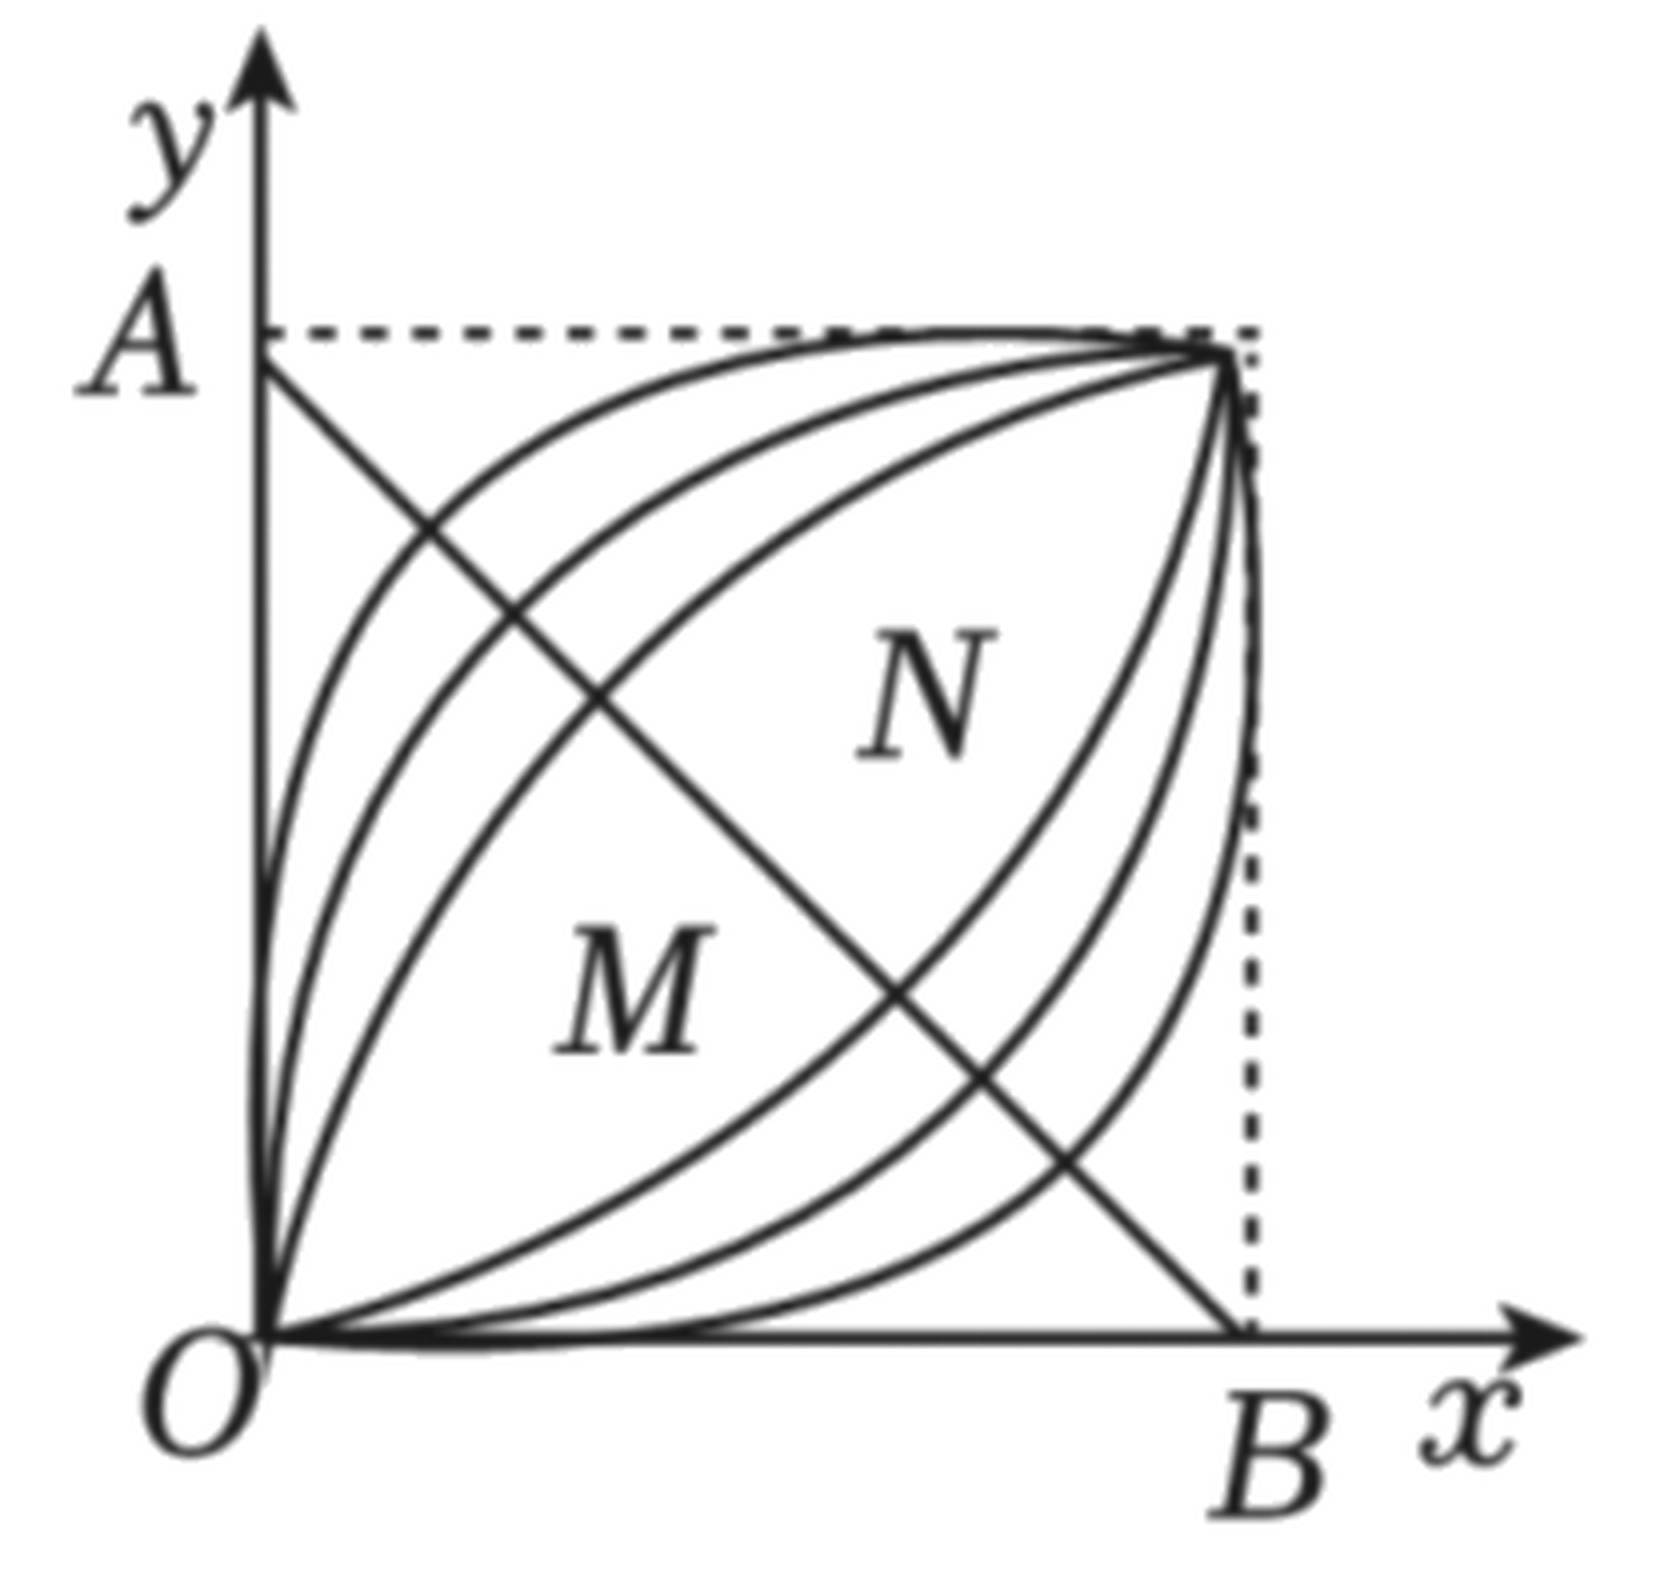
\includegraphics[width=0.40\textwidth]{figures/gao148_q12.png}
\end{center}

\ifanswer
\solbegin
\step{$BM=MN=NA$，点 $A(1,0)$，$B(0,1)$，所以 $M\left(\dfrac{1}{3},\dfrac{2}{3}\right)$，$N\left(\dfrac{2}{3},\dfrac{1}{3}\right)$，}
\step{分别代入 $y=x^\alpha$，$y=x^\beta$，$\alpha=\log_{\frac{2}{3}}\dfrac{1}{3},\beta=\log_{\frac{1}{3}}\dfrac{2}{3}$，$\alpha\beta=\log_{\frac{1}{3}}\dfrac{2}{3}\cdot\log_{\frac{2}{3}}\dfrac{1}{3}=1$.}
\solend
\fi

\end{enumerate}

\bigsec{二、选择题}

\begin{enumerate}
\setcounter{enumi}{12}

% === Q13 ===：答案"C"直接印在题干括号内、全卷无该题【答案】/【解析】段，按 高一84 Q13 成例括号留空、另提 \ans{$C$}；弯引号含空格
\item 若 $x$、$y\in\R$，则 “ $x=0$ ” 是 “ $xy=0$ ” 的\mbox{（\quad）}

\keepwithprev
A. 充要条件\qquad\qquad B. 必要不充分条件

C. 充分不必要条件\qquad\qquad D. 既不充分也不必要条件

\ifanswer
\ans{$C$}
\fi

% === Q14 ===：六个结论（圈数字在文本模式）、四选项一行；解析 8 行（对② 的两行公式各占一印刷行）
\item 若 $a<b<0$，下面有六个结论：① $a^2>b^2$；② $a^3<b^3$；③ $\dfrac{1}{a}<\dfrac{1}{b}$；④ $\dfrac{a}{b}>1$；⑤ $\dfrac{1}{a-b}>\dfrac{1}{a}$；⑥ $\lvert a\rvert>-b$. 其中正确的个数是\mbox{（\quad）}

\keepwithprev
A. 1\qquad\qquad B. 2\qquad\qquad C. 3\qquad\qquad D. 4

\ifanswer
\solbegin
\step{对①：$a^2-b^2=(a+b)(a-b),a+b<0,a-b<0$，故 $a^2-b^2>0$，正确；}
\step{对②：$a^3-b^3=(a-b)(a^2+ab+b^2)=(a-b)\left[\left(a+\dfrac{1}{2}b\right)^2+\dfrac{3}{4}b^2\right],a-b<0$，}
\step{$\left(a+\dfrac{1}{2}b\right)^2+\dfrac{3}{4}b^2>0$，故 $a^3-b^3<0$，正确；}
\step{对③：取 $a=-2,b=-1$，则 $\dfrac{1}{a}=-\dfrac{1}{2},\dfrac{1}{b}=-1,\dfrac{1}{a}>\dfrac{1}{b}$，错误；}
\step{对④：$\dfrac{a}{b}-1=\dfrac{a-b}{b},a-b<0,b<0$，故 $\dfrac{a}{b}-1>0$，正确；}
\step{对⑤：取 $a=-2,b=-1$，则 $\dfrac{1}{a-b}=-1,\dfrac{1}{a}=-\dfrac{1}{2},\dfrac{1}{a-b}<\dfrac{1}{a}$，错误；}
\step{对⑥：要证 $\lvert a\rvert>-b$，即 $-a>-b$，即 $a<b$，正确；}
\step{故选 $D$.}
\solend
\fi

% === Q15 ===：题目配图（四条指数函数曲线，三版都出），\needvspace 守卫放 \item 之前；"图象"照录；解析 5 行
\needvspace{8cm}
\item 如图，曲线①②③④分别是指数函数 $y=a^x$，$y=b^x$，$y=c^x$，$y=d^x$ 的图象，则实数 $a$、$b$、$c$、$d$ 的大小关系为\mbox{（\quad）}

\keepwithprev
A. $a<b<c<d$\qquad B. $b<a<d<c$\qquad C. $d<c<b<a$\qquad D. $c<d<a<b$

\begin{center}
% 四条指数函数曲线图取 04 页右侧，去粉色水印、去色、4× LANCZOS 放大；三版都出
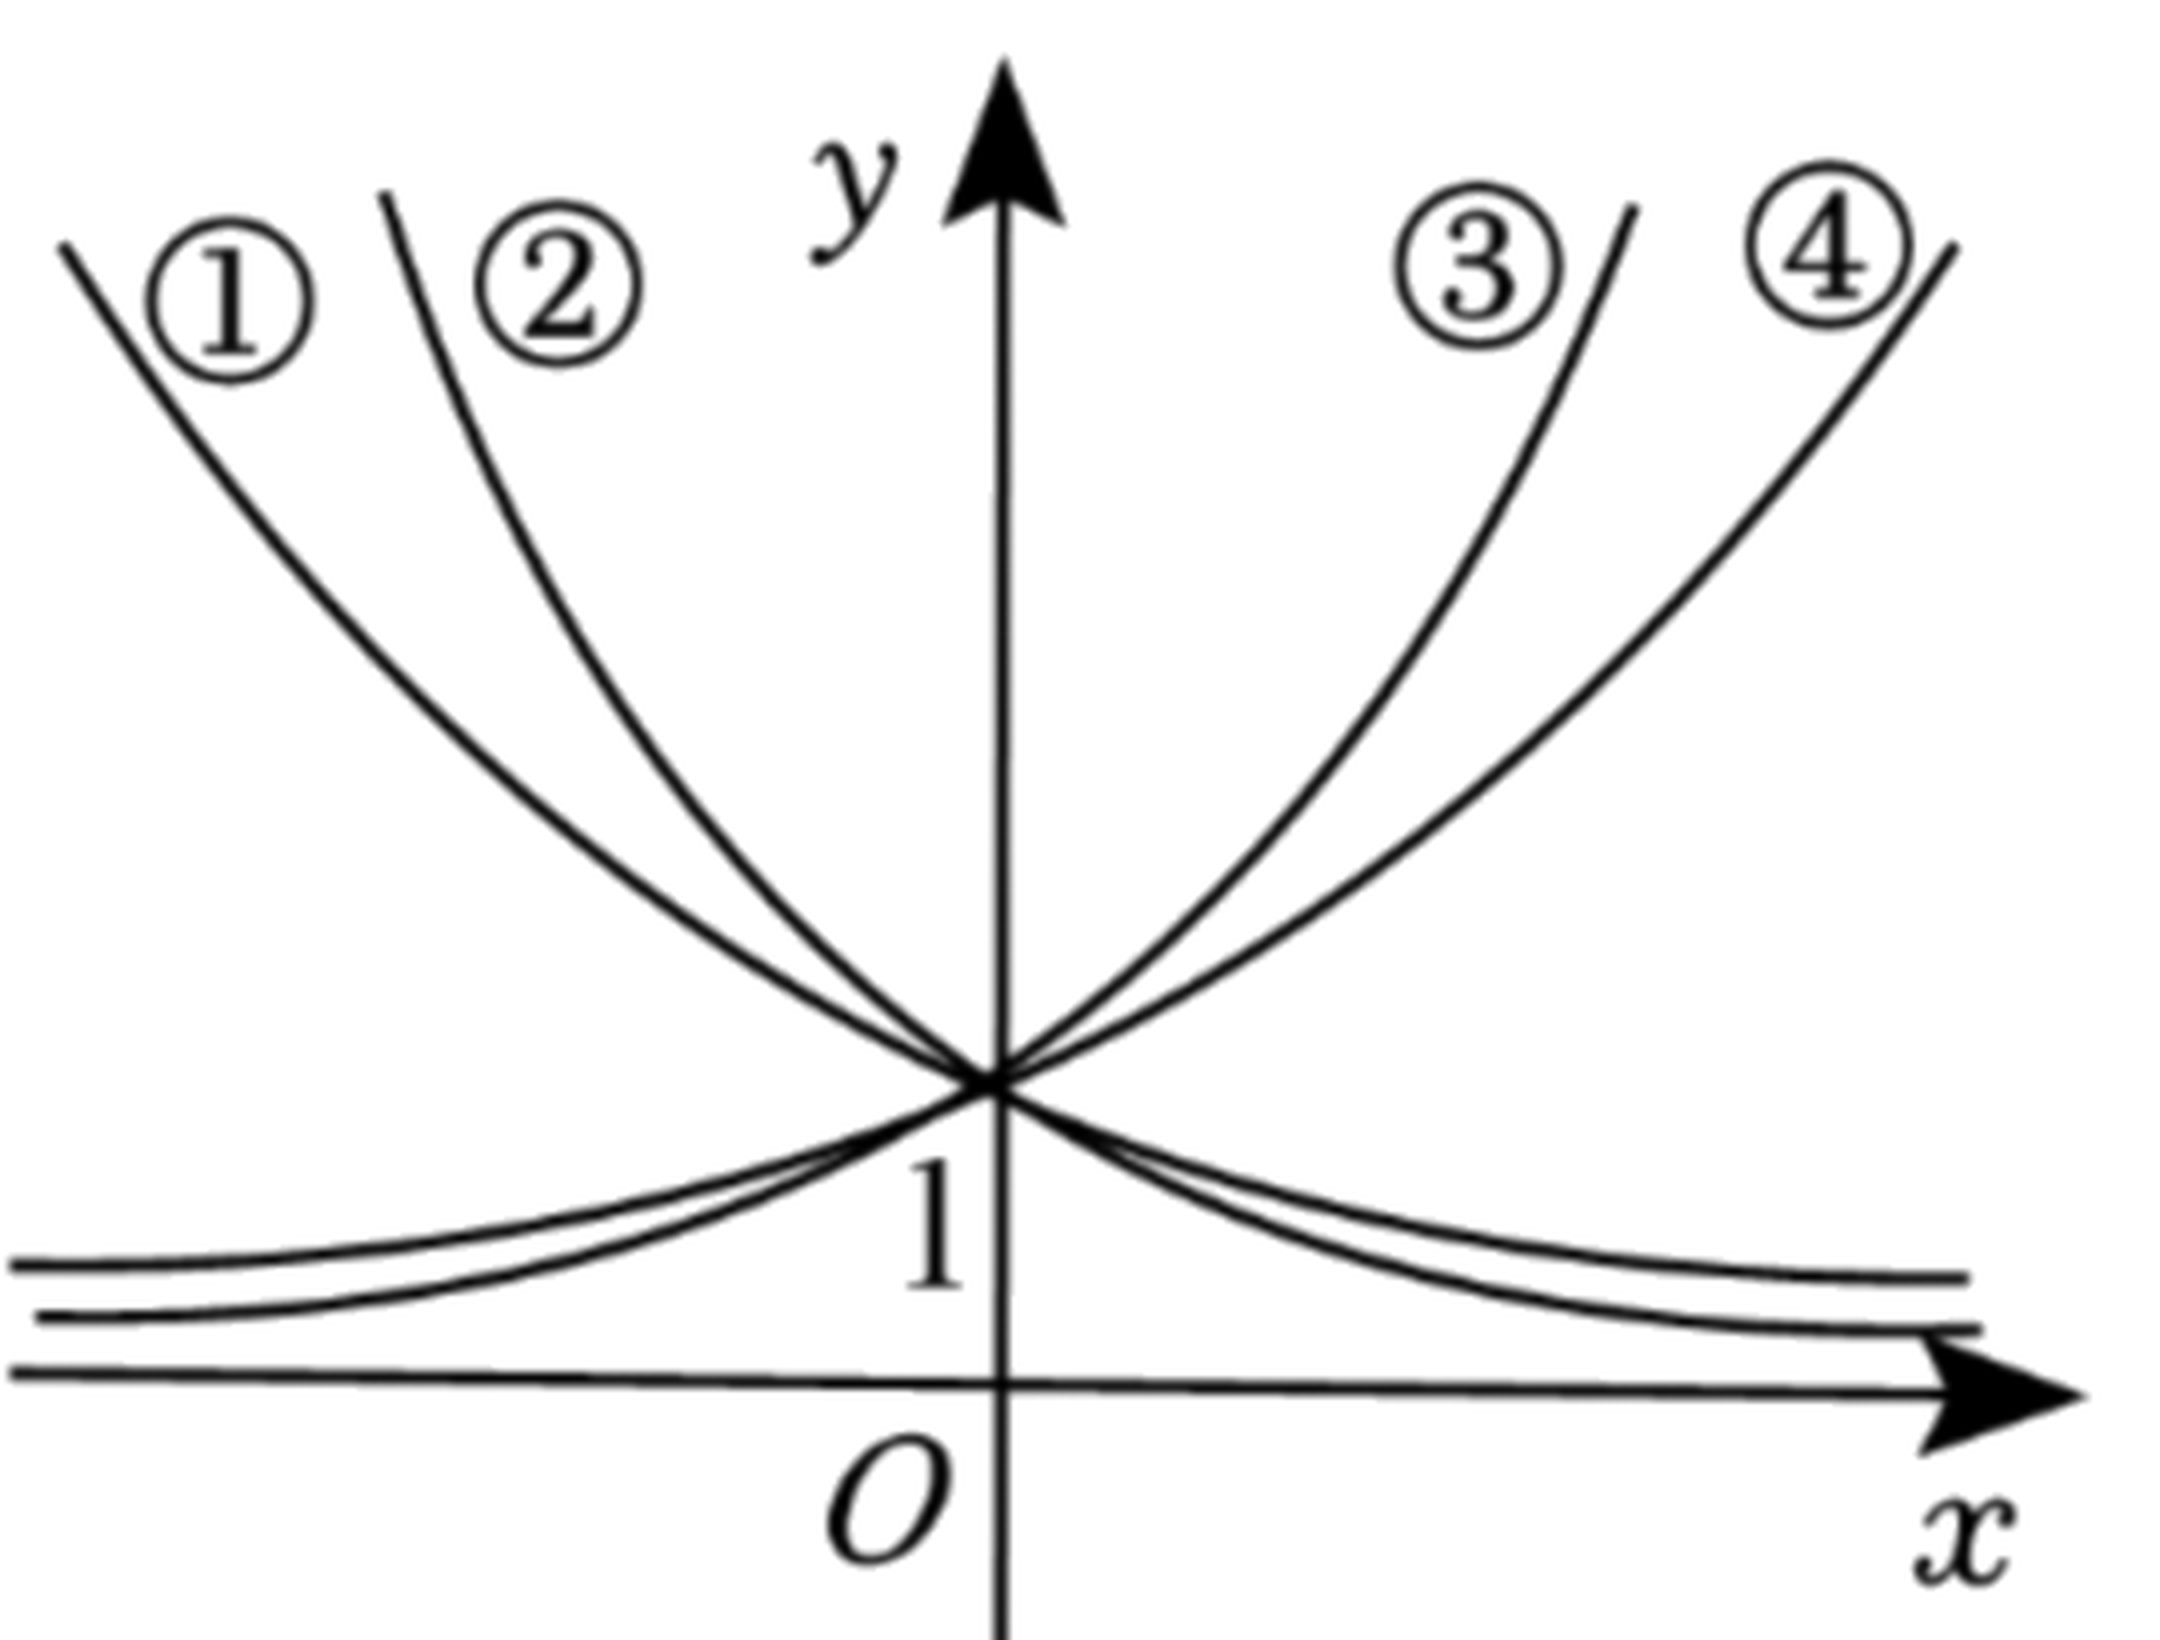
\includegraphics[width=0.40\textwidth]{figures/gao148_q15.png}
\end{center}

\ifanswer
\solbegin
\step{由函数图象得函数① $y=a^x$；② $y=b^x$ 为减函数，且 $x=1$ 时，$b^1<a^1$，}
\step{所以 $0<b<a<1$，}
\step{由函数图象得函数③ $y=c^x$；④ $y=d^x$ 为增函数，且 $x=1$ 时，$c^1>d^1$，}
\step{所以 $c>d>1$，}
\step{所以 $b<a<d<c$. 故选 $B$.}
\solend
\fi

% === Q16 ===：题目配图（关于 y 轴对称的幂函数曲线，三版都出），\needvspace 守卫放 \item 之前；$p$、$q\in\Z$；"图象"照录；解析 2 行
\needvspace{8cm}
\item 已知幂函数 $y=x^{\frac{p}{q}}$（$p$、$q\in\Z$ 且 $p$、$q$ 互质）的图象关于 $y$ 轴对称，如图所示，则\mbox{（\quad）}

\keepwithprev
A. $p$、$q$ 均为奇数，且 $\dfrac{p}{q}>0$\qquad\qquad B. $q$ 为偶数，$p$ 为奇数，且 $\dfrac{p}{q}<0$

C. $q$ 为奇数，$p$ 为偶数，且 $\dfrac{p}{q}>0$\qquad\qquad D. $q$ 为奇数，$p$ 为偶数，且 $\dfrac{p}{q}<0$

\begin{center}
% 关于 y 轴对称的幂函数曲线图取 04 页右下，去粉色水印、去色、4× LANCZOS 放大；三版都出
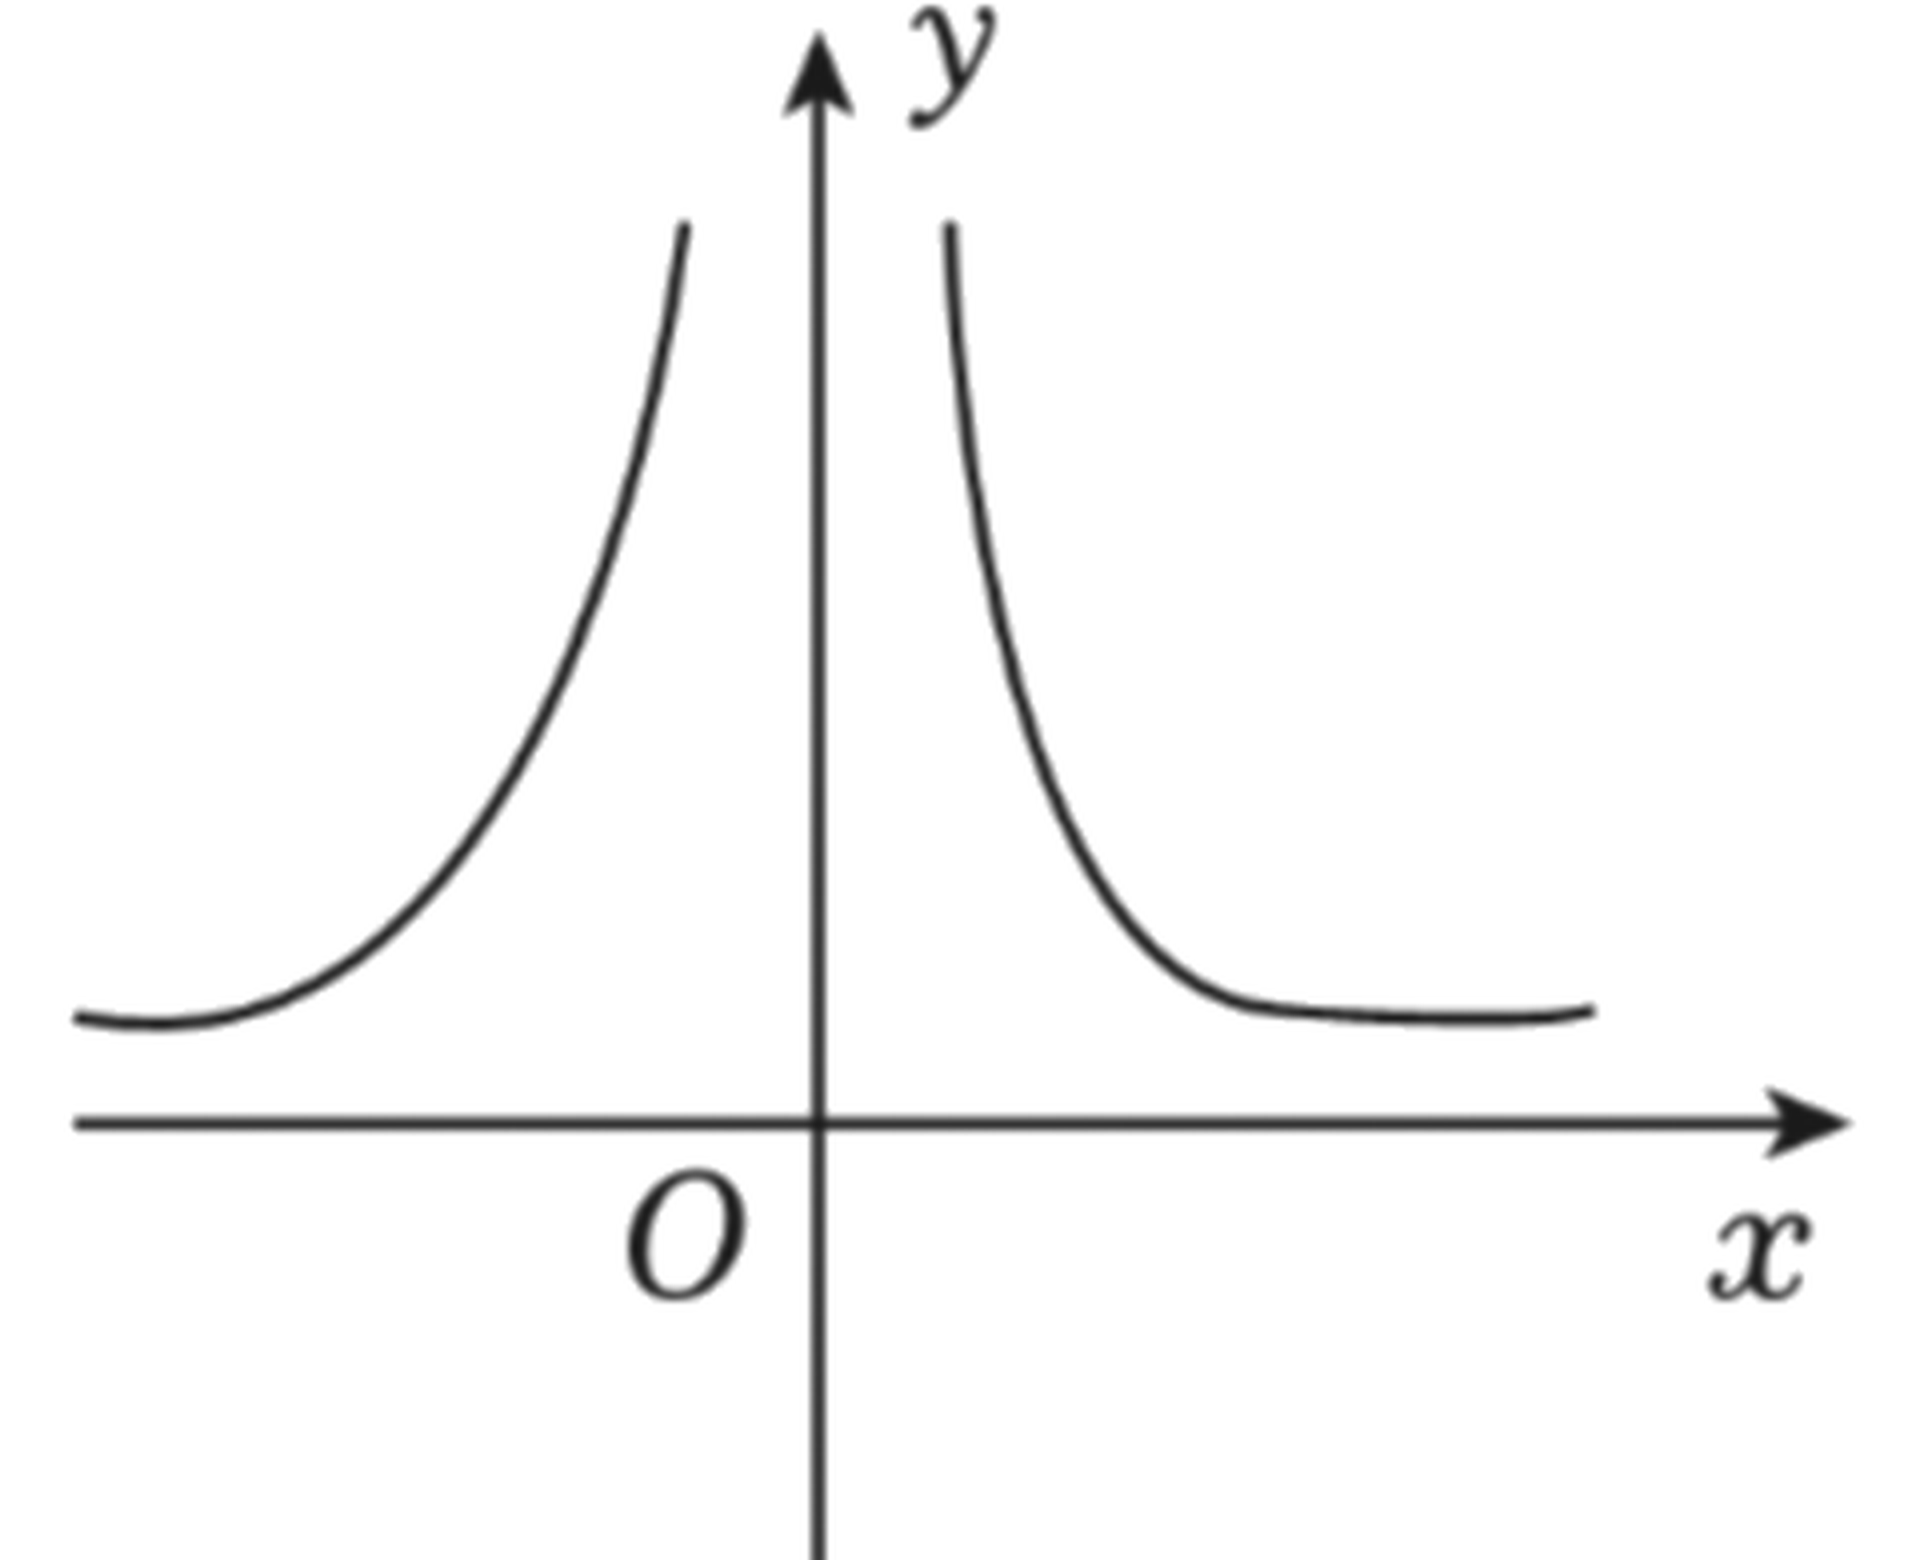
\includegraphics[width=0.36\textwidth]{figures/gao148_q16.png}
\end{center}

\ifanswer
\solbegin
\step{因为函数为偶函数，所以 $p$ 为偶数，且由图象形状判定 $\dfrac{p}{q}<0$.}
\step{又 $p$、$q$ 互质，所以 $q$ 为奇数. 故选 $D$.}
\solend
\fi

\end{enumerate}

\bigsec{三、解答题}

\begin{enumerate}
\setcounter{enumi}{16}

% === Q17 ===：\overline{B}／\varnothing／\R／\mid 逐处照录；解析 8 行
\item 已知集合 $A=\left\{x\mid \dfrac{5}{2x+1}>1\right\}$，$B=\{x\mid x^2+(a+3)x+3a<0,a\in\R\}$.

(1) 求 $A$.

(2) 若全集 $U=\R$，且 $A\cap\overline{B}=\varnothing$，求实数 $a$ 的取值范围.

\ifanswer
\solbegin
\step{(1) $\dfrac{5}{2x+1}>1$，即 $\dfrac{5}{2x+1}-1>0$，即 $\dfrac{4-2x}{2x+1}>0$，即 $(2x+1)(x-2)<0$，}
\step{解得 $-\dfrac{1}{2}<x<2$，所以 $A=\left(-\dfrac{1}{2},2\right)$；}
\step{(2) $x^2+(a+3)x+3a<0$，即 $(x+3)(x+a)<0$，}
\step{全集 $U=\R$，且 $A\cap\overline{B}=\varnothing$，}
\step{当 $a<3$ 时，解得 $-3<x<-a$，则 $\overline{B}=(-\infty,-3)\cup(-a,+\infty)$，}
\step{此时 $-a\geqslant2$，解得 $a\leqslant-2$，}
\step{当 $a\geqslant3$ 时，不满足 $A\cap\overline{B}=\varnothing$，}
\step{故实数 $a$ 的取值范围是 $(-\infty,-2]$.}
\solend
\fi

% === Q18 ===：cases 块整体算一个印刷行；解析 6 行
\item 已知幂函数经过点 $(2,4)$.

(1) 当 $x=\dfrac{1}{2}$ 时，求函数的值；

(2) 是否存在实数 $m$、$n$，使得该函数在区间 $[m,n]$ 上最小值为 $6m-8$，最大值为 $6n-8$？若存在，求出 $m$、$n$ 的值，若不存在，请说明理由.

\ifanswer
\solbegin
\step{(1) 设幂函数的解析式是 $y=x^\alpha$，则 $2^\alpha=4$，解得 $\alpha=2$，}
\step{故 $f(x)=x^2$，$f\left(\dfrac{1}{2}\right)=\dfrac{1}{4}$；}
\step{(2) 因为 $f(x)\geqslant0$，所以 $6m-8\geqslant0$，$m\geqslant\dfrac{4}{3}$，}
\step{由函数 $f(x)$ 在 $(0,+\infty)$ 严格增，得函数 $f(x)$ 在 $(m,n)$ 严格增，}
\step{所以 $\begin{cases}f(m)=6m-8\\f(n)=6n-8\end{cases}$ 且 $m<n$，解得 $m=2$，$n=4$，}
\step{故存在 $m=2$，$n=4$ 满足题意.}
\solend
\fi

% === Q19 ===：7 处评分档照 高一54／64 成例排 \dots\dots N 分；判别式高 \Delta；解析 9 行
\item 已知方程 $x^2+6mx+9m-2=0$，且 $x_1,x_2$ 是方程的两个不同的实数根.

(1) 若 $m=1$，求 $\dfrac{1}{x_1}+\dfrac{1}{x_2}$ 的值；

(2) 若 $m\in\R$，且 $x_1^2+x_2^2<4$，求 $m$ 取值范围.

\ifanswer
\solbegin
\step{(1) 当 $m=1$ 时，方程为 $x^2+6x+7=0$，\dots\dots1 分}
\step{则 $x_1+x_2=-6,x_1\cdot x_2=7$，\dots\dots2 分}
\step{$\dfrac{1}{x_1}+\dfrac{1}{x_2}=\dfrac{x_1+x_2}{x_1\cdot x_2}=-\dfrac{6}{7}$\dots\dots3 分}
\step{(2) $x_1+x_2=-6m,x_1\cdot x_2=9m-2$\dots\dots2 分}
\step{因为 $x_1^2+x_2^2=(x_1+x_2)^2-2x_1\cdot x_2$，所以 $(x_1+x_2)^2-2x_1\cdot x_2<4$，}
\step{所以 $36m^2-2(9m-2)<4$，解得 $0<m<\dfrac{1}{2}$\dots\dots2 分}
\step{又因为方程有两个不同的根，所以 $\Delta=36m^2-4(9m-2)>0$，}% 判别式原卷印等腰偏高粗三角 $\Delta$，照录（放大 07 页 q19_delta3.png／diag_band_q19.png 确认）
\step{解得 $m<\dfrac{1}{3}$ 或 $m>\dfrac{2}{3}$\dots\dots2 分}
\step{所以 $0<m<\dfrac{1}{3}$\dots\dots2 分}
\solend
\fi

% === Q20 ===：题目配图（矩形蔬菜温室，三版都出），\needvspace 守卫放 \item 之前；单位 \mathrm{m}／\mathrm{m}^2；解析 10 行
\needvspace{8cm}
\item 某村计划建造一个室内面积为 $600\mathrm{m}^2$ 的矩形蔬菜温室，在室内，沿左、右两侧与后侧内墙各保留 $2\mathrm{m}$ 宽的通道，沿前侧内墙保留 $4\mathrm{m}$ 宽的空地.

\begin{center}
% 矩形蔬菜温室示意图取 07 页右侧，去粉色水印、去色、4× LANCZOS 放大；三版都出
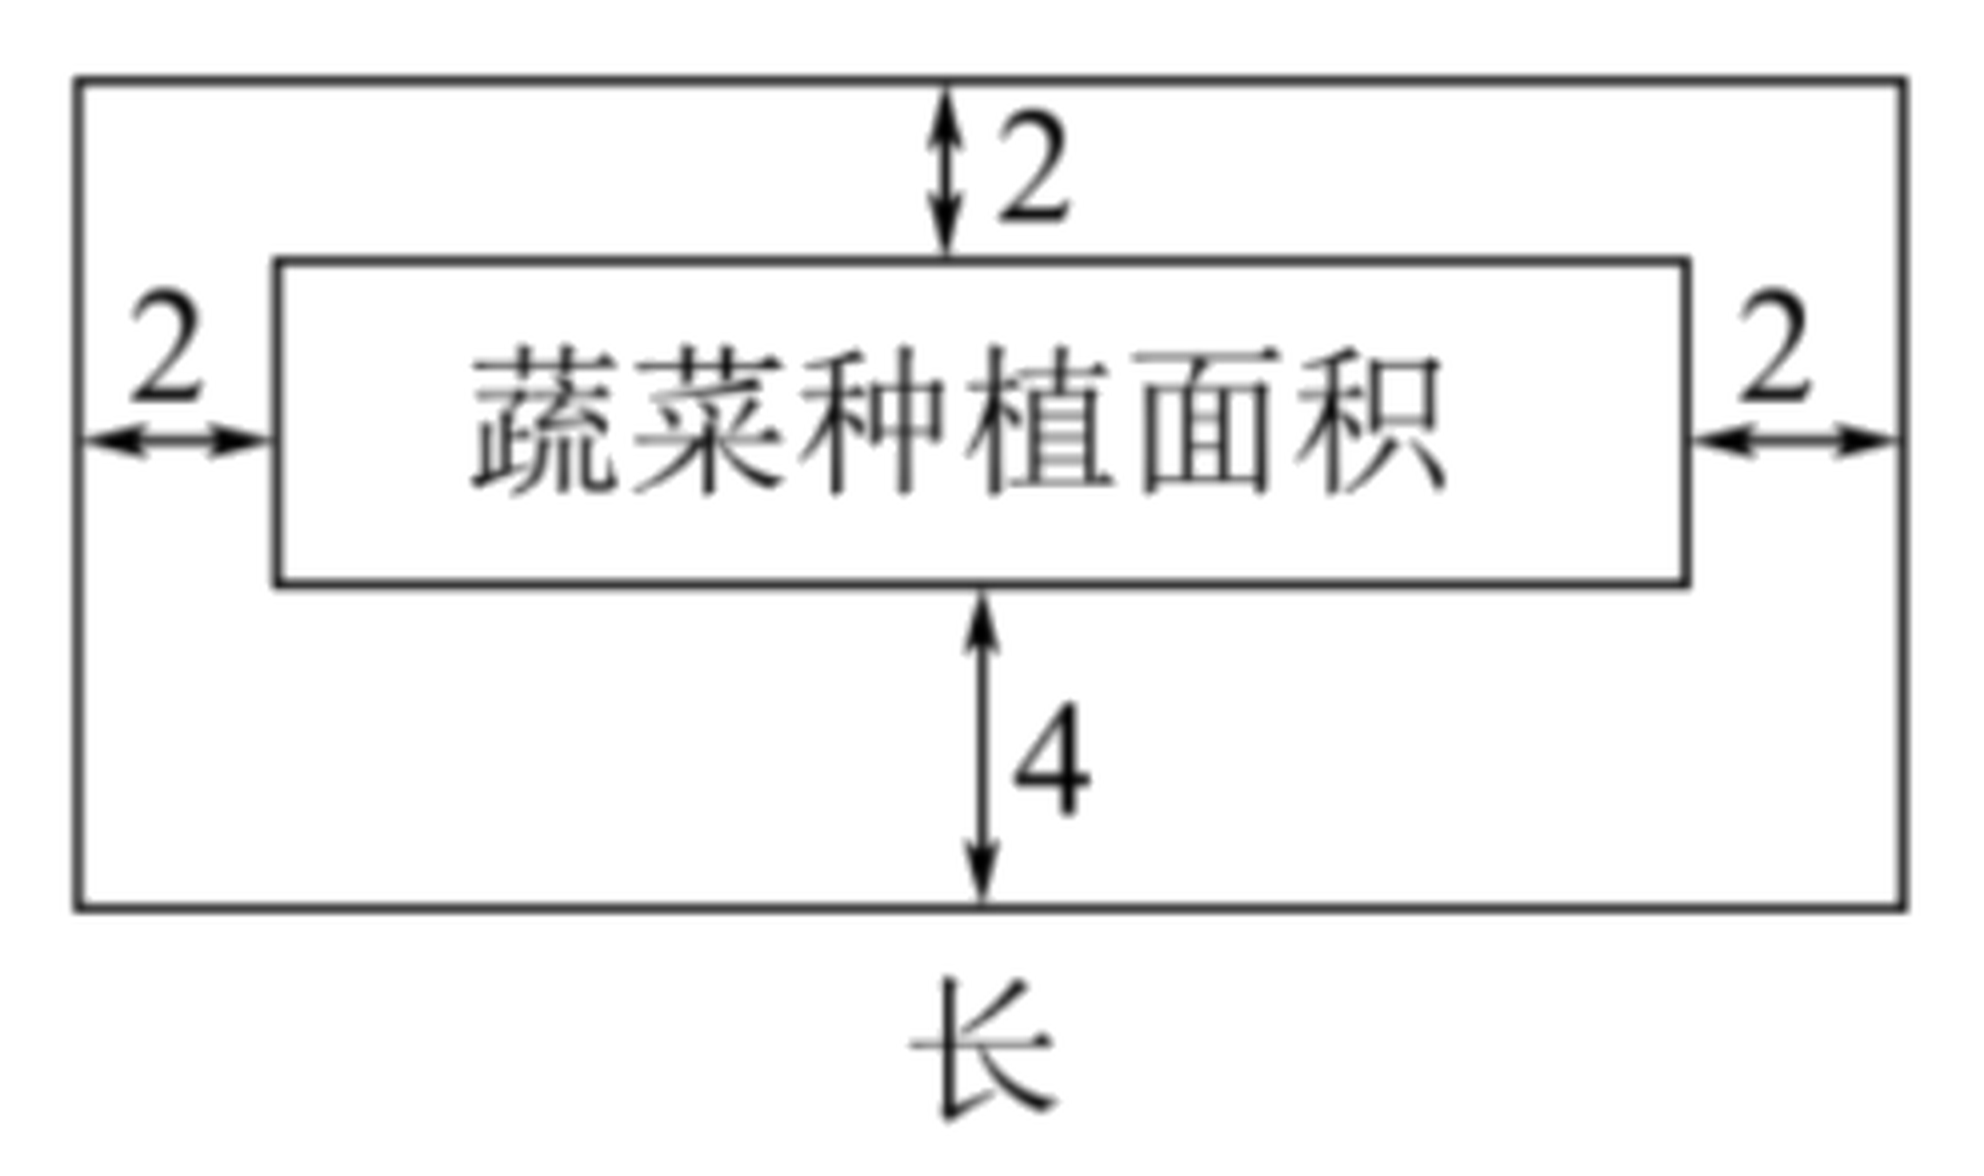
\includegraphics[width=0.45\textwidth]{figures/gao148_q20.png}
\end{center}

(1) 写出蔬菜的种植面积关于矩形温室的长之间的关系式.

(2) 当矩形温室的边长各为多少时，蔬菜的种植面积最大？最大种植面积是多少？

\ifanswer
\solbegin
\step{(1) 设蔬菜的种植面积为 $y\mathrm{m}^2$，矩形温室的长为 $x\mathrm{m}$，}
\step{则矩形温室的宽为 $\dfrac{600}{x}\mathrm{m}$，}
\step{种植蔬菜矩形的长为 $(x-4)\mathrm{m}$，宽为 $\left(\dfrac{600}{x}-6\right)\mathrm{m}$，}
\step{所以 $y=(x-4)\left(\dfrac{600}{x}-6\right)(4<x<100)$；}
\step{(2) 因为 $y=(x-4)\left(\dfrac{600}{x}-6\right)=624-\left(6x+\dfrac{2400}{x}\right)$，}
\step{因为 $6x+\dfrac{2400}{x}\geqslant2\sqrt{6x\cdot\dfrac{2400}{x}}=240$，}
\step{当且仅当 $6x=\dfrac{2400}{x}$，即 $x=20$ 时取等号，}
\step{所以 $y=624-\left(6x+\dfrac{2400}{x}\right)\leqslant624-240=384$.}
\step{即当矩形温室的一边长为 $20\mathrm{m}$，另一边长为 $30\mathrm{m}$ 时，}
\step{蔬菜的种植面积最大，最大为 $384\mathrm{m}^2$.}
\solend
\fi

% === Q21 ===：3 问、cases 块整体算一个印刷行；判别式高 \Delta；解析 19 行（末行续 09 页）
\item 二次函数 $f(x)=ax^2+bx+c$ 满足对任意的 $x\in\R$，$x-1\leqslant f(x)\leqslant x^2-x$ 恒成立.

(1) 求证：$f(1)$ 为定值；

(2) 若 $f(0)=-\dfrac{1}{4}$，求二次函数 $f(x)$ 的表达式；

(3) 求 $a+2b+5c$ 的取值范围.

\ifanswer
\solbegin
\step{(1) 对任意的 $x\in\R$，$x-1\leqslant f(x)\leqslant x^2-x$ 恒成立，则 $0\leqslant f(1)\leqslant0$，}
\step{所以 $f(1)=0$，为定值.}
\step{(2) 由(1)得 $a+b+c=f(1)=0$，由 $f(0)=-\dfrac{1}{4}$，得 $c=-\dfrac{1}{4}$，}
\step{则 $b=\dfrac{1}{4}-a$，$f(x)=ax^2+\left(\dfrac{1}{4}-a\right)x-\dfrac{1}{4}$，}
\step{不等式 $x-1\leqslant f(x)$ 可化为 $ax^2+\left(\dfrac{1}{4}-a\right)x-\dfrac{1}{4}\geqslant x-1$，}
\step{即 $ax^2-\left(a+\dfrac{3}{4}\right)x+\dfrac{3}{4}\geqslant0$，}
\step{一元二次不等式 $ax^2-\left(\dfrac{3}{4}+a\right)x+\dfrac{3}{4}\geqslant0$ 恒成立，则 $\begin{cases}a>0\\\Delta=\left(a+\dfrac{3}{4}\right)^2-3a\leqslant0\end{cases}$，}% 判别式原卷印等腰偏高粗三角 $\Delta$，照录（放大 08 页 q21_delta3.png／diag_band_q21.png 确认）
\step{解得 $a=\dfrac{3}{4}$，}
\step{此时 $f(x)=\dfrac{3}{4}x^2-\dfrac{1}{2}x-\dfrac{1}{4}$，$x^2-x-f(x)=\dfrac{1}{4}(x-1)^2\geqslant0$ 恒成立，}
\step{所以 $f(x)=\dfrac{3}{4}x^2-\dfrac{1}{2}x-\dfrac{1}{4}$.}
\step{(3) 由(1)得 $b=-a-c$，$f(x)=ax^2-(a+c)x+c=(ax-c)(x-1)$，}
\step{不等式 $x-1\leqslant f(x)$ 可化为 $(x-1)(ax-c-1)\geqslant0$，}
\step{一元二次不等式 $(x-1)(ax-c-1)\geqslant0$ 恒成立，则 $a>0$，}
\step{且方程 $(x-1)(ax-c-1)=0$ 有相等的实数根，因此 $c=a-1$，$a>0$，}
\step{不等式 $f(x)\leqslant x^2-x\Leftrightarrow(ax-c)(x-1)\leqslant x^2-x\Leftrightarrow(x-1)[(1-a)x+c]\geqslant0$，}
\step{同理 $1-a>0$，且方程 $(x-1)[(1-a)x+c]=0$ 有相等的实数根，}
\step{因此 $c=a-1$，$a<1$，从而 $c=a-1$，$b=1-2a$，$0<a<1$，}
\step{$a+2b+5c=a+2(1-2a)+5(a-1)=2a-3\in(-3,-1)$，}
\step{所以 $a+2b+5c$ 的取值范围是 $(-3,-1)$.}
\solend
\fi

\end{enumerate}

\end{document}
"
%
% ① 原始材料：微信公众号"魔都数学加油站"文章，连载"27学年高一148"，原文标题
% "27学年高一148——2026-2027年上海市新川中学高一上期中"（2026-11-21 推送）；
% 原文链接：https://mp.weixin.qq.com/s/Alhmwb3sSLQMp_wjzoAVyA 。
% 正文为 9 张 PNG 页（01/03/04/07/08/09 为 2560×3620，02/05/06 为 4762×6735，
% 同一篇各页分辨率混排，逐页按各自分辨率裁图核对，别按预览比例换算裁框）。
% 体例：混合体例讲评版——19 题中 Q4、Q5 只印【答案】、无【解析】；Q13 的答案"C"
% 直接印在题干括号内、无【答案】/【解析】段；其余 16 题印【解析】（逐题核实，见 ② ②）。
% 题目、答案、解析均据原图转录；卷面粉红色水印"魔都数学加油站"及公众号页脚未录入。
% 全卷插图清单（逐页通读 9 页确认）：4 幅题目配图，均三版都出、均非【解析】内配图：
%   · Q12 幂函数曲线族图（03 页右侧：x/y 轴、O、A(1,0)、B(0,1)、M、N 与两族
%     y=x^α／y=x^β 曲线、线段 AB、虚线），题干"（如图）"处，裁 figures/gao148_q12.png；
%   · Q15 四条指数函数曲线图（04 页右侧：①②③④ 四曲线同过 (0,1)、x/y 轴、O、
%     y 轴刻度 1），题干"如图"处，裁 figures/gao148_q15.png；
%   · Q16 关于 y 轴对称的幂函数曲线图（04 页右下：x/y 轴、O、两支上翘曲线），
%     题干"如图所示"处，裁 figures/gao148_q16.png；
%   · Q20 矩形蔬菜温室示意图（07 页右侧：大矩形＋内框"蔬菜种植面积"＋2/2/4
%     通道标注＋"长"），题干处，裁 figures/gao148_q20.png；
%   其余各页逐页确认无其它题目配图、无【解析】内配图、无表格，亦无"题干写如图而
%   源码漏图"一处；Q19 解析行末的虚线"----N 分"为评分档（非图），Q18／Q21 的
%   cases 块为数学块（非图）。4 图均取自原卷截图，去粉色水印、去色、4× LANCZOS 放大。
%
% 卷首标题：原卷印作"2026-2027 年新川中学高一上期中"，年份区间按全稿惯例排 en dash；
% 原卷卷面未印副标题，本稿按同期中卷（高一140／141／143／144／145／146／147）知识模块
% 口径补出"集合与常用逻辑用语、不等式、函数"。
%
% 题号体例（逐页核实定稿）：本卷共 19 题——一、填空题 3—12（10 题）、
% 二、选择题 13—16（4 题）、三、解答题 17—21（5 题）。
% 三节分别 \setcounter{enumi}{2}／{12}／{16}。原卷从第 3 题起、无第 1、2 题，
% 本稿保留原题号；全卷无附加题节、无 Q22（Q21 解析末行"所以 a+2b+5c 的取值范围是
% (-3,-1)."为全卷收尾，09 页下半仅水印、无正文）。
%
% ② 与原卷的排版差异：
%   ① 原文从第 3 题起，本稿保留原题号；共 19 题三节；
%   ② 混合体例逐题核实：Q4（反证法"假设的内容"）、Q5 只印【答案】、无【解析】，
%      按 高一140 第 5 题／高一145 Q3 成例提 \ans{}、不补造解析；Q13 答案"C"直接
%      印在题干括号内（" ( C ) "）、全卷无该题【答案】/【解析】段，按 高一84 Q13／
%      高一37 Q13／高一53 Q13 成例括号 \mbox{（\quad）} 留空、另提 \ans{$C$}；
%      其余 16 题印【解析】、用 \solbegin…\solend，选择题答案在解析末句"故选 X"
%      （Q14 选 D、Q15 选 B、Q16 选 D，逐个放大原图核实）、题干括号留空、不另提
%      \ans{}；答案版【答案】/【解析】标记数 = 19（3 个 \ans ＋ 16 个 \solbegin）
%      = 全卷题数；
%   ③ 原卷卷面未印副标题，本稿按知识模块口径补出；
%   ④ 原卷填空横线按全稿惯例排 \blankline[4.4em]；选择题括号排 \mbox{（\quad）}、
%      选项段前按惯例加 \keepwithprev；Q13／Q16 四选项为两行两列、Q14／Q15 选项
%      为一行，照原卷分行；解答题不留作答区、不加 \anspace（原卷为讲评版，
%      与 129／131／132／133／136／140／141／143／144／145／146 同）；
%   ⑤ 数集：Q11"在 R 上定义运算"、Q13"x、y∈R"、Q16"p、q∈Z"、Q17"a∈R"
%      "U=R"、Q19"m∈R"、Q21"x∈R" 原卷印斜体 R/Z，按全稿惯例统一改 \R／\Z
%      （本卷未出现 N，\N^* 无对应处）；绝对值排 \lvert…\rvert（Q9／Q14），
%      集合描述竖线排 \mid（Q17）；不等号按全稿惯例排 \leqslant／\geqslant；
%      补集照原卷上划线排 \overline{B}（Q17 题干 1 处＋解析 3 处）；空集
%      \varnothing（Q17 题干 1 处＋解析 2 处）；\subset（Q3 题干 {a}⊂M）与
%      \subseteq（Q3 题干 M⊆{a,b,c,d}）逐处照录不统一（放大 01 页 q3_subset.png）；
%   ⑥ 子题标号 (1)(2)(3) 半角括号照录；圈数字 ①—⑥ 在文本模式（Q14 六个结论、
%      Q15 曲线编号与其解析、Q14 解析"对①…对⑥"），按 common.sty 划入 CJK 字符类
%      渲染；cases 块整体算一个印刷行；\left…\right 不得拆到不同 $…$ 组；
%      单位 m／m² 排 \mathrm{m}／\mathrm{m}^2（Q20，原卷印正体 m）；
%   ⑦ 题干／解析中的中文弯引号按原卷照录：Q4" ab 可以被 5 整除，那么 a、b 中
%      至少有一个能被 5 整除 "（开引号后有空格、闭引号后空格接"时"）、
%      Q13" x=0 "" xy=0 "（引号内空格），注释内一律 ASCII 引号；
%   ⑧ 半角逗号在数学组之间是全稿惯例、非笔误（Q3"{a,b,c,d}"、Q6"$x,y$"
%      "$x=\frac13,y=\frac16$"、Q10、Q11"$a=-2,b=-1"、Q12"$\alpha=\log..,\beta=..$"、
%      Q14"$a+b<0,a-b<0$"、Q17、Q19"$x_1+x_2=-6,x_1\cdot x_2=7$"、Q20、Q21 等），
%      逐处照录别改全角；行末西文句点照录为 ASCII `.`；行中全角逗号／顿号照录；
%   ⑨ "图像／图象"逐处放大核：全卷 9 处均印"图象"（象，无亻）、未见"图像"，
%      逐处照录未统一改动（Q8 题干/解析各 1、Q12 题干 2、Q15 题干 1／解析 2、
%      Q16 题干 1／解析 1；放大 02/03/04/05 页 /tmp/gao148/zoom/my_wide_a.png、
%      my_wide_b.png 与宋体参考"象／像"并排确认）；
%   ⑩ 判别式 Δ/△ 混用是照录项：Q11 解析"△=1−4(−a²+a+1)<0"印扁等边空心
%      三角 \triangle；Q19 解析"Δ=36m²−4(9m−2)>0"、Q21 解析 cases 块
%      "Δ=(a+3/4)²−3a≤0" 两处印等腰偏高粗三角 \Delta，逐处放大判断、照录
%      不统一（参照 高一142／144／145 头注④口径，详见 ④）；
%   ⑪ 一条 \step = 原卷解析的一个印刷行，cases 块整体算一个印刷行；别把原卷折行
%      并起来、别把一行拆多条。Q3 六行、Q7 五行（01 页末首行＋02 页顶四行）、
%      Q9 七行、Q11 五行、Q14 八行（对② 的两行公式各占一印刷行）、Q17 八行、
%      Q18 六行、Q19 九行（7 处评分档附在行末）、Q20 十行、Q21 十九行
%      均按印刷行逐条断，不丢行；
%   ⑫ 配图：4 幅均为题目配图（三版都出），放 \item 内题干之后 \begin{center}；
%      大图块加 \needvspace 守卫把整块推走（守卫放 \item 之前，见 高一145 Q14/Q20
%      成例与切页审计 B 类坑）；三版切页审计均"合计异常：无"；
%   ⑬ 跨页续印按题合并：Q3/4/5 在 01 页；Q6 题干＋解析在 01 页；Q7 题干在 01 页
%      末、解析首行在 01 页末续 02 页顶四行；Q8/9/10 在 02 页（Q9 解析续 02 页下半、
%      Q10 题干与解析前 2 行在 02 页末）；Q10 解析末行续 03 页顶；Q11/12 在 03 页、
%      "二、选择题"标题与 Q13/14 题干在 03 页下半；Q13 无解析；Q14 解析在 04 页顶、
%      Q15 题干＋图＋选项＋解析在 04 页、Q16 题干＋图在 04 页末；Q16 选项＋解析＋
%      "三、解答题"标题＋Q17 题干＋解析在 05 页、Q18 题干首句在 05 页末；Q18 题干
%      续＋解析、Q19 题干＋解析前 5 行在 06 页；Q19 解析续 4 行＋Q20 题干＋图＋
%      解析（10 行全部）在 07 页，末行"蔬菜的种植面积最大，最大为 384m²."收尾；
%      Q21 题干＋解析前 18 行在 08 页；Q21 解析末行"所以 a+2b+5c 的取值范围是
%      (-3,-1)."在 09 页上半（09 页下半仅水印、无正文）。本稿按题连排，不丢行、
%      不并折行；
%   ⑭ 原卷解析内无红色"法一／法二"之类小标题，故本卷无 \stepm；水印
%      "魔都数学加油站"红色不录入；Q19 解析 7 处评分档（1/2/3/2/2/2/2 分）
%      原卷在行末印一串虚线，本稿照 高一54／64 成例排 \dots\dots N 分，
%      分值逐处照录、位置不变。
%
% ③ 行数复核：一条 \step／\stepm = 原卷解析的一个印刷行，cases 块作一个印刷行计。
%   逐题数（主会话逐页核对定稿）：Q3：6；Q4：0（只印【答案】、提 \ans{}）；
%   Q5：0（只印【答案】、提 \ans{}）；Q6：2；Q7：5；Q8：2；Q9：7；Q10：3；
%   Q11：5；Q12：2；Q13：0（答案印在题干括号内、另提 \ans{}）；Q14：8；Q15：5；
%   Q16：2；Q17：8；Q18：6；Q19：9；Q20：10；Q21：19。
%   合计 99 条 \step（本卷无 \stepm：解析内无红色"法一／法二"类小标题），
%   与原卷逐题印刷行相等。全卷 16 题设 \solbegin…\solend ＋ 3 处 \ans{}，
%   答案版【答案】/【解析】标记数 = 19 = 全卷题数。
%
% ④ 判别式／子集符号结论（逐处放大原图照录、不得统一，主会话像素级复核）：
%   判别式全卷 3 处，两形混用逐处照录不统一（参照 高一142／144／145 头注④口径）：
%     · Q11 解析"△=1−4(−a²+a+1)<0" 原卷印扁等边空心三角（宽>高、细线），
%       照录 \triangle（放大 03 页 /tmp/gao148/zoom/q11_delta3.png、
%       delta_montage.png 确认）；
%     · Q19 解析"Δ=36m²−4(9m−2)>0" 原卷印等腰偏高粗三角（高>宽），
%       照录 \Delta（放大 07 页 /tmp/gao148/zoom/q19_delta3.png 确认）；
%     · Q21 解析 cases 块"Δ=(a+3/4)²−3a≤0" 原卷印等腰偏高粗三角（高>宽），
%       照录 \Delta（放大 08 页 /tmp/gao148/zoom/q21_delta3.png 确认）。
%   子集／补集：Q3 题干"{a}⊂M⊆{a,b,c,d}" 前者印单线 ⊂、无下划线，照录 \subset；
%     后者印带下划线 ⊆，照录 \subseteq（放大 01 页 /tmp/gao148/zoom/q3_subset.png
%     确认）；Q17 题干 1 处＋解析 3 处共 4 处 \overline{B} 照原卷上划线
%     （B 上横线、非 C_U B）；空集 \varnothing 3 处（Q17 题干 1 处、解析 2 处）；
%     Q17 集合描述竖线 \mid；数集 \R／\Z 归一见 ② ⑤。
%
% ⑤ 存疑照录（放大原图确认，照录未改、正文对应处另有 % 注）：
%   1. Q3 解析末行"所以 M 一共有 3+3+1+1=8 个" 原卷印 $3+3+1+1=8$，按上文
%      四行应为 $1+3+3+1=8$（疑为原卷加数顺序笔误，和仍为 8），放大 01 页
%      /tmp/gao148/zoom/my_q3_sol.png 确认，照录未改。
%   2. Q13 答案"C"直接印在题干括号内、全卷无该题【答案】/【解析】段，按
%      高一84 Q13 成例括号留空、另提 \ans{$C$}（见 ② ②），未补造解析。
%   3. Q19 解析 7 处评分档（"----N 分"）原卷印一串虚线，本稿照 高一54／64
%      成例排 \dots\dots N 分，分值逐处照录、位置不变。
%   4. 判别式 Q11 扁 \triangle 与 Q19／Q21 高 \Delta 两形混用，逐处照录不统一（见 ④）。
%   5. "图像／图象"全卷 9 处均印"图象"、未见"图像"（见 ② ⑨），逐处放大核实照录，
%      未统一改动。
%   全卷除此 5 类外未发现其它笔误／自相矛盾处。
%
% ⑥ 跨页续印按题合并说明：见 ② ⑬。
%
\documentclass[a4paper,11pt]{article}
\usepackage{common}

\begin{document}

\examtitlest[3]{2026--2027 年新川中学高一上期中}{集合与常用逻辑用语、不等式、函数}

\bigsec{一、填空题}

\begin{enumerate}
\setcounter{enumi}{2}

% === Q3 ===：题干 {a}⊂M⊆{a,b,c,d} 两个子集符号逐处照录；解析 6 行
\item 满足 $\{a\}\subset M\subseteq\{a,b,c,d\}$ 的集合 $M$ 有\blankline[4.4em]个.

\ifanswer
\solbegin
\step{$M$ 是 $\{a,b,c,d\}$ 的子集，但必含有元素 $a$，}
\step{当 $M$ 中只一个元素时，$M=\{a\}$ 只有 1 个；}
\step{当 $M$ 中有二个元素时，$M$ 有 3 个；}
\step{当 $M$ 中有三个元素时，$M$ 有 3 个；}
\step{当 $M$ 中有四个元素时，$M$ 有 1 个；}
\step{所以 $M$ 一共有 $3+3+1+1=8$ 个.}% 原卷印 $3+3+1+1=8$（按上文四行应为 $1+3+3+1$），疑为加数顺序笔误，照录未改（放大 01 页 my_q3_sol.png）
\solend
\fi

% === Q4 ===：原卷只印【答案】、无【解析】，按 高一140 第 5 题成例提 \ans{}；弯引号与空格照录
\item 用反证法证明命题 “ $ab$ 可以被 5 整除，那么 $a$、$b$ 中至少有一个能被 5 整除” 时假设的内容应该是\blankline[4.4em].

\ifanswer
\ans{$a$、$b$ 都不能被 5 整除}
\fi

% === Q5 ===：原卷只印【答案】 $[-2,1)$、无【解析】，提 \ans{}
\item 不等式 $\dfrac{x+2}{x-1}\leqslant0$ 的解集为\blankline[4.4em].

\ifanswer
\ans{$[-2,1)$}
\fi

% === Q6 ===：解析 2 行；半角逗号在数学组之间照录
\item 设 $x,y\in(0,+\infty)$，且 $x+4y=1$，则 $\dfrac{1}{x}+\dfrac{1}{y}$ 的最小值为\blankline[4.4em].

\ifanswer
\solbegin
\step{因为 $\dfrac{1}{x}+\dfrac{1}{y}=(x+4y)\left(\dfrac{1}{x}+\dfrac{1}{y}\right)=5+\dfrac{4y}{x}+\dfrac{x}{y}\geqslant5+2\sqrt{\dfrac{4y}{x}\cdot\dfrac{x}{y}}=9$，}
\step{当且仅当 $\dfrac{4y}{x}=\dfrac{x}{y}$，即 $x=2y$，即 $x=\dfrac{1}{3},y=\dfrac{1}{6}$ 时取等号，故最小值为 9.}
\solend
\fi

% === Q7 ===：题干在 01 页末、解析首行在 01 页末续 02 页顶四行；解析 5 行
\item 若不等式 $x^2+ax+b<0$ 的解集为 $(-3,-1)$，则不等式 $bx^2+ax+1\leqslant0$ 的解集为\blankline[4.4em].

\ifanswer
\solbegin
\step{不等式 $x^2+ax+b<0$ 的解集为 $(-3,-1)$，}
\step{所以方程 $x^2+ax+b=0$ 的两个实数根为 $-3$ 和 $-1$，}
\step{由根与系数的关系得 $a=4$，$b=3$，}
\step{故 $bx^2+ax+1\leqslant0$ 可化为 $3x^2+4x+1\leqslant0$，解得 $-1\leqslant x\leqslant-\dfrac{1}{3}$，}
\step{所求不等式 $bx^2+ax+1\leqslant0$ 的解集为 $\left[-1,-\dfrac{1}{3}\right]$.}
\solend
\fi

% === Q8 ===："图象"照录；解析 2 行
\item 函数 $y=a^{x-2}+2(a>0,a\ne1)$ 的图象必经过定点\blankline[4.4em].

\ifanswer
\solbegin
\step{令 $x-2=0$，得 $x=2$，则 $y=a^0+2=3$，}
\step{所以函数 $y=a^{x-2}+2$ 的图象过定点 $(2,3)$.}
\solend
\fi

% === Q9 ===：解析 7 行；首句末西文句点照录
\item 不等式 $\lvert x+3\rvert+\lvert a-x\rvert>6$ 对一切实数 $x$ 恒成立，则实数 $a$ 的取值范围为\blankline[4.4em].

\ifanswer
\solbegin
\step{$\lvert x+3\rvert$ 表示 $x$ 到 $-3$ 的距离，$\lvert a-x\rvert$ 表示 $x$ 到 $a$ 的距离.}
\step{所以它们的和为 $x$ 到 $-3$ 和 $x$ 到 $a$ 的距离之和，}
\step{当 $x$ 位于 $-3$ 和 $a$ 之间时，距离和取得最小值，}
\step{即两点之间的距离 $\lvert a-(-3)\rvert=\lvert a+3\rvert$，}
\step{若最小值 $\lvert a+3\rvert>6$，则原式对所有 $x$ 恒成立.}
\step{解得 $a+3>6$ 或 $a+3<-6$，即 $a>3$ 或 $a<-9$，}
\step{故 $a\in(3,+\infty)$ 或 $a\in(-\infty,-9)$.}
\solend
\fi

% === Q10 ===：题干与解析前 2 行在 02 页末、解析末行续 03 页顶；解析 3 行
\item 已知 $2^a=3$，$\log_3 5=b$，则 $\log_{15}20=$\blankline[4.4em]（用 $a$、$b$ 表示）.

\ifanswer
\solbegin
\step{因为 $2^a=3$，所以 $a=\log_2 3=\dfrac{\lg3}{\lg2}$，又 $\log_3 5=b=\dfrac{\lg5}{\lg3}$，}
\step{所以 $\lg3=a\lg2$，$\lg5=b\lg3=ba\lg2$，}
\step{则 $\log_{15}20=\dfrac{2\lg2+\lg5}{\lg3+\lg5}=\dfrac{2\lg2+ab\lg2}{a\lg2+ab\lg2}=\dfrac{2+ab}{a+ab}$.}
\solend
\fi

% === Q11 ===：在 \R 上定义运算 \otimes；判别式扁 \triangle 照录；解析 5 行
\item 在 $\R$ 上定义运算 $\otimes:x\otimes y=x(1-y)$，若不等式 $(x-a)\otimes(x+a)<1$ 对任意实数 $x$ 恒成立，则 $a$ 的取值范围是\blankline[4.4em].

\ifanswer
\solbegin
\step{由题意得不等式 $(x-a)\otimes(x+a)<1$ 对任意实数 $x$ 恒成立，}
\step{即不等式 $(x-a)(1-x-a)<1$ 对任意实数 $x$ 恒成立，}
\step{即 $x^2-x-a^2+a+1>0$ 对任意实数 $x$ 恒成立，}
\step{所以 $\triangle=1-4(-a^2+a+1)<0$，解得 $-\dfrac{1}{2}<a<\dfrac{3}{2}$，}% 判别式原卷印扁等边空心三角 $\triangle$，照录（放大 03 页 q11_delta3.png 确认）
\step{所以实数 $a$ 的取值范围为 $\left(-\dfrac{1}{2},\dfrac{3}{2}\right)$.}
\solend
\fi

% === Q12 ===：题目配图（幂函数曲线族，三版都出）；"图象"照录；解析 2 行
\needvspace{8cm}
\item 幂函数 $y=x^\alpha$，当 $\alpha$ 取不同的正数时，在区间 $[0,1]$ 上它们的图象是一族美丽的曲线（如图）. 设点 $A(1,0)$，$B(0,1)$，连接 $AB$，线段 $AB$ 恰好被其中的两个幂函数 $y=x^\alpha$，$y=x^\beta$ 的图象三等分，即有 $BM=MN=NA$，那么 $\alpha\beta=$\blankline[4.4em].

\begin{center}
% 幂函数曲线族图取 03 页右侧，去粉色水印、去色、4× LANCZOS 放大；三版都出
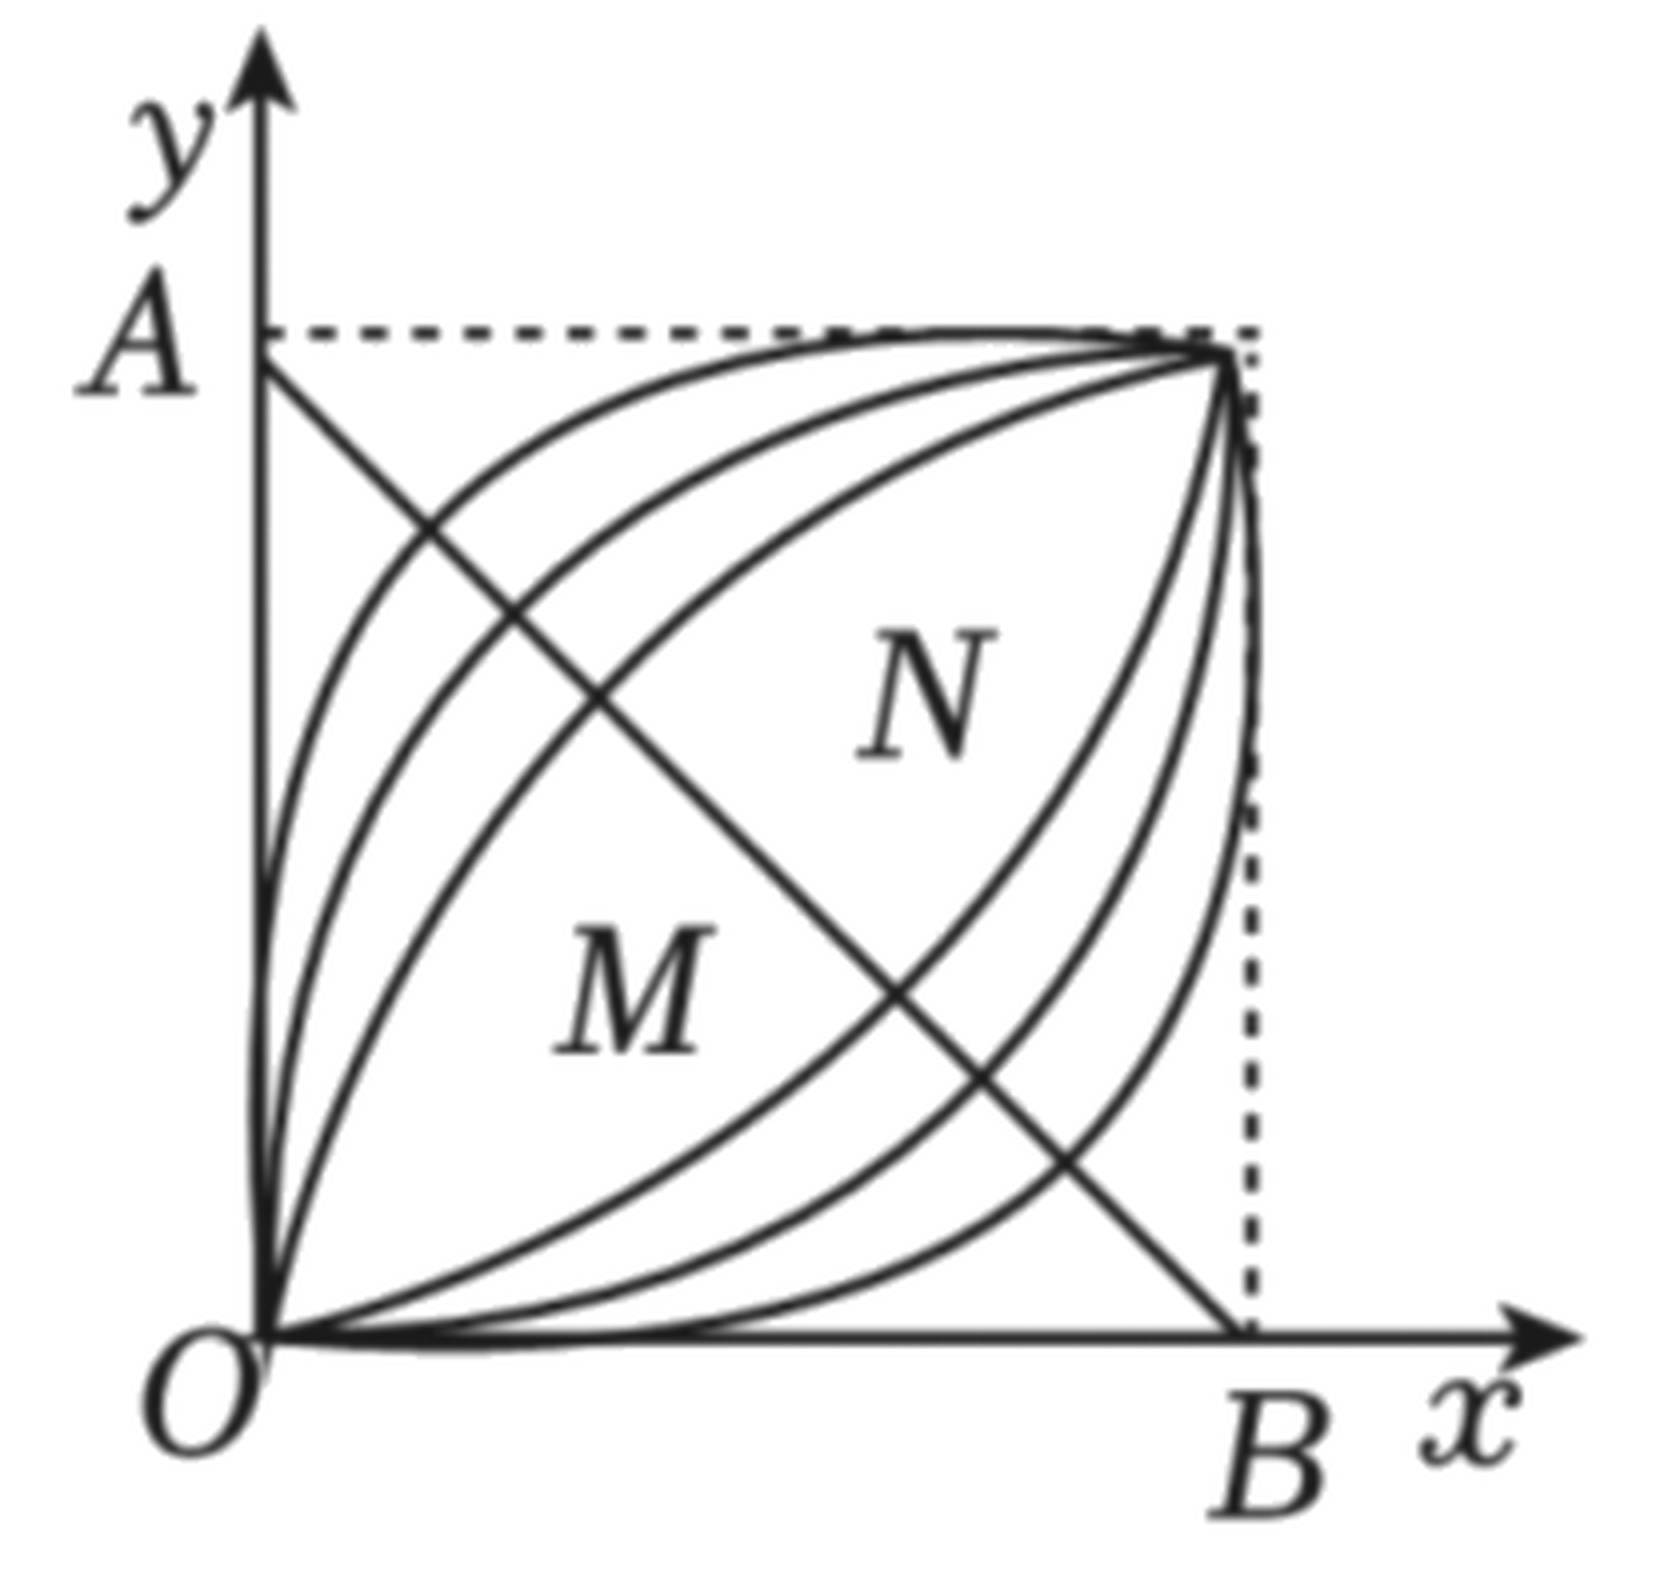
\includegraphics[width=0.40\textwidth]{figures/gao148_q12.png}
\end{center}

\ifanswer
\solbegin
\step{$BM=MN=NA$，点 $A(1,0)$，$B(0,1)$，所以 $M\left(\dfrac{1}{3},\dfrac{2}{3}\right)$，$N\left(\dfrac{2}{3},\dfrac{1}{3}\right)$，}
\step{分别代入 $y=x^\alpha$，$y=x^\beta$，$\alpha=\log_{\frac{2}{3}}\dfrac{1}{3},\beta=\log_{\frac{1}{3}}\dfrac{2}{3}$，$\alpha\beta=\log_{\frac{1}{3}}\dfrac{2}{3}\cdot\log_{\frac{2}{3}}\dfrac{1}{3}=1$.}
\solend
\fi

\end{enumerate}

\bigsec{二、选择题}

\begin{enumerate}
\setcounter{enumi}{12}

% === Q13 ===：答案"C"直接印在题干括号内、全卷无该题【答案】/【解析】段，按 高一84 Q13 成例括号留空、另提 \ans{$C$}；弯引号含空格
\item 若 $x$、$y\in\R$，则 “ $x=0$ ” 是 “ $xy=0$ ” 的\mbox{（\quad）}

\keepwithprev
A. 充要条件\qquad\qquad B. 必要不充分条件

C. 充分不必要条件\qquad\qquad D. 既不充分也不必要条件

\ifanswer
\ans{$C$}
\fi

% === Q14 ===：六个结论（圈数字在文本模式）、四选项一行；解析 8 行（对② 的两行公式各占一印刷行）
\item 若 $a<b<0$，下面有六个结论：① $a^2>b^2$；② $a^3<b^3$；③ $\dfrac{1}{a}<\dfrac{1}{b}$；④ $\dfrac{a}{b}>1$；⑤ $\dfrac{1}{a-b}>\dfrac{1}{a}$；⑥ $\lvert a\rvert>-b$. 其中正确的个数是\mbox{（\quad）}

\keepwithprev
A. 1\qquad\qquad B. 2\qquad\qquad C. 3\qquad\qquad D. 4

\ifanswer
\solbegin
\step{对①：$a^2-b^2=(a+b)(a-b),a+b<0,a-b<0$，故 $a^2-b^2>0$，正确；}
\step{对②：$a^3-b^3=(a-b)(a^2+ab+b^2)=(a-b)\left[\left(a+\dfrac{1}{2}b\right)^2+\dfrac{3}{4}b^2\right],a-b<0$，}
\step{$\left(a+\dfrac{1}{2}b\right)^2+\dfrac{3}{4}b^2>0$，故 $a^3-b^3<0$，正确；}
\step{对③：取 $a=-2,b=-1$，则 $\dfrac{1}{a}=-\dfrac{1}{2},\dfrac{1}{b}=-1,\dfrac{1}{a}>\dfrac{1}{b}$，错误；}
\step{对④：$\dfrac{a}{b}-1=\dfrac{a-b}{b},a-b<0,b<0$，故 $\dfrac{a}{b}-1>0$，正确；}
\step{对⑤：取 $a=-2,b=-1$，则 $\dfrac{1}{a-b}=-1,\dfrac{1}{a}=-\dfrac{1}{2},\dfrac{1}{a-b}<\dfrac{1}{a}$，错误；}
\step{对⑥：要证 $\lvert a\rvert>-b$，即 $-a>-b$，即 $a<b$，正确；}
\step{故选 $D$.}
\solend
\fi

% === Q15 ===：题目配图（四条指数函数曲线，三版都出），\needvspace 守卫放 \item 之前；"图象"照录；解析 5 行
\needvspace{8cm}
\item 如图，曲线①②③④分别是指数函数 $y=a^x$，$y=b^x$，$y=c^x$，$y=d^x$ 的图象，则实数 $a$、$b$、$c$、$d$ 的大小关系为\mbox{（\quad）}

\keepwithprev
A. $a<b<c<d$\qquad B. $b<a<d<c$\qquad C. $d<c<b<a$\qquad D. $c<d<a<b$

\begin{center}
% 四条指数函数曲线图取 04 页右侧，去粉色水印、去色、4× LANCZOS 放大；三版都出
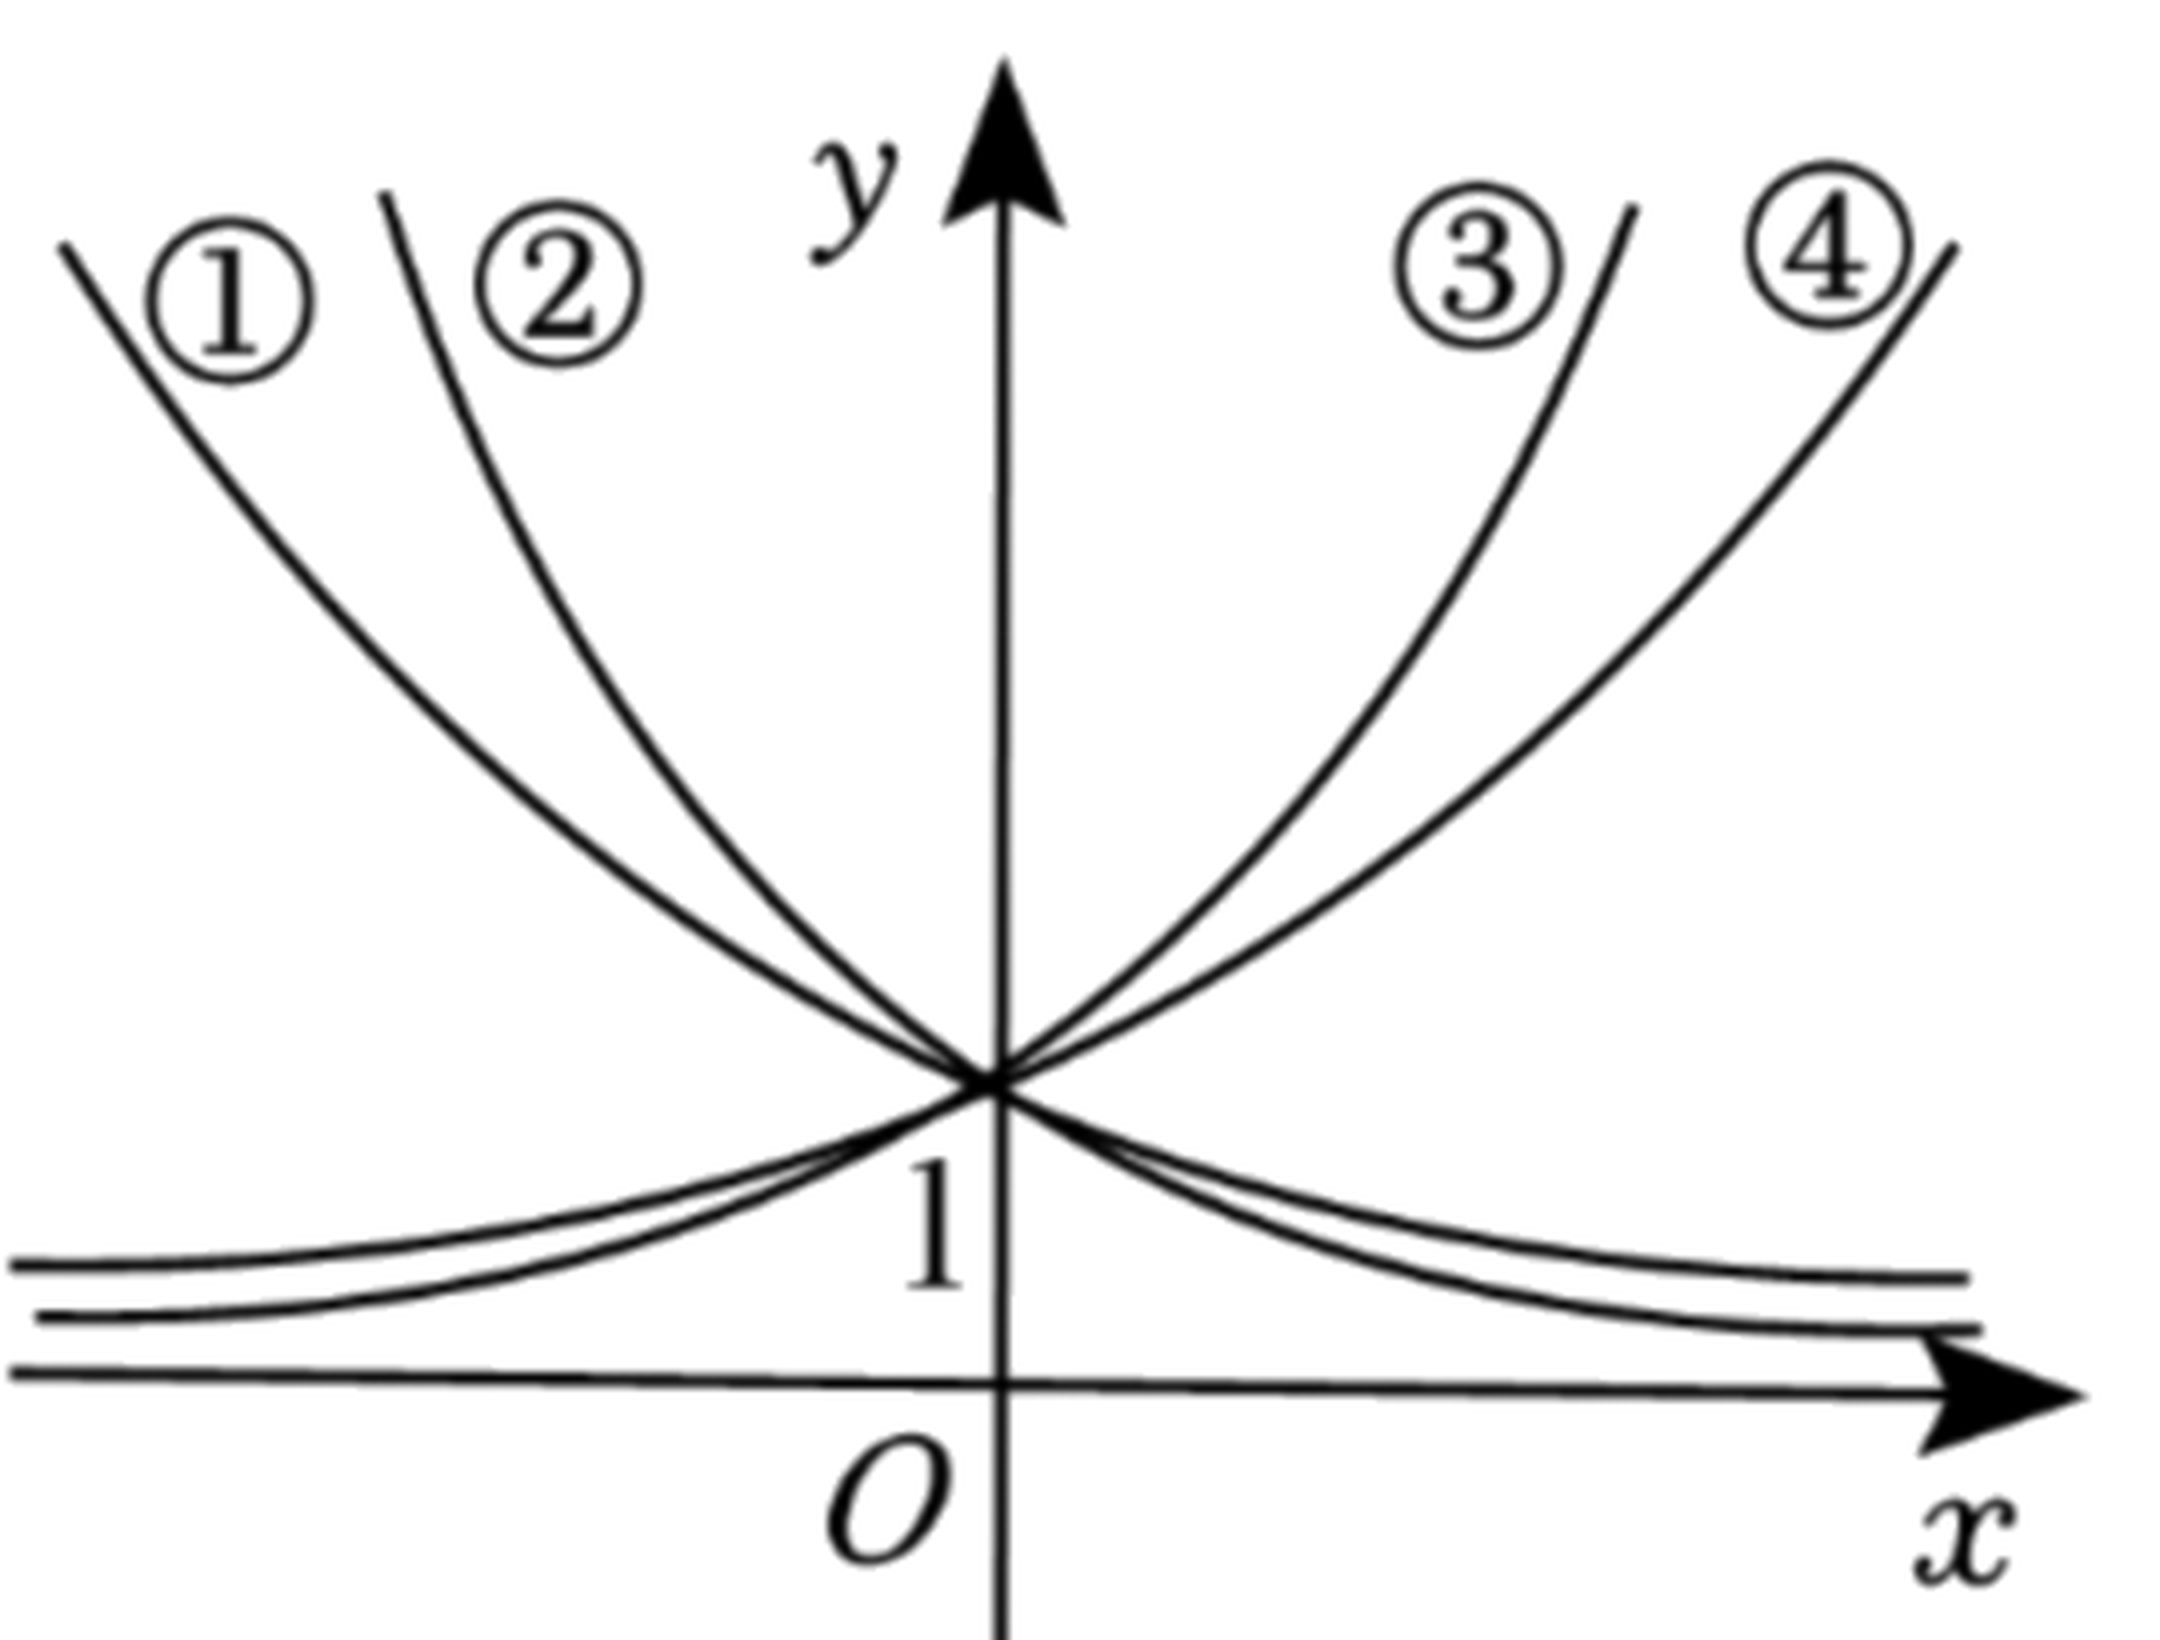
\includegraphics[width=0.40\textwidth]{figures/gao148_q15.png}
\end{center}

\ifanswer
\solbegin
\step{由函数图象得函数① $y=a^x$；② $y=b^x$ 为减函数，且 $x=1$ 时，$b^1<a^1$，}
\step{所以 $0<b<a<1$，}
\step{由函数图象得函数③ $y=c^x$；④ $y=d^x$ 为增函数，且 $x=1$ 时，$c^1>d^1$，}
\step{所以 $c>d>1$，}
\step{所以 $b<a<d<c$. 故选 $B$.}
\solend
\fi

% === Q16 ===：题目配图（关于 y 轴对称的幂函数曲线，三版都出），\needvspace 守卫放 \item 之前；$p$、$q\in\Z$；"图象"照录；解析 2 行
\needvspace{8cm}
\item 已知幂函数 $y=x^{\frac{p}{q}}$（$p$、$q\in\Z$ 且 $p$、$q$ 互质）的图象关于 $y$ 轴对称，如图所示，则\mbox{（\quad）}

\keepwithprev
A. $p$、$q$ 均为奇数，且 $\dfrac{p}{q}>0$\qquad\qquad B. $q$ 为偶数，$p$ 为奇数，且 $\dfrac{p}{q}<0$

C. $q$ 为奇数，$p$ 为偶数，且 $\dfrac{p}{q}>0$\qquad\qquad D. $q$ 为奇数，$p$ 为偶数，且 $\dfrac{p}{q}<0$

\begin{center}
% 关于 y 轴对称的幂函数曲线图取 04 页右下，去粉色水印、去色、4× LANCZOS 放大；三版都出
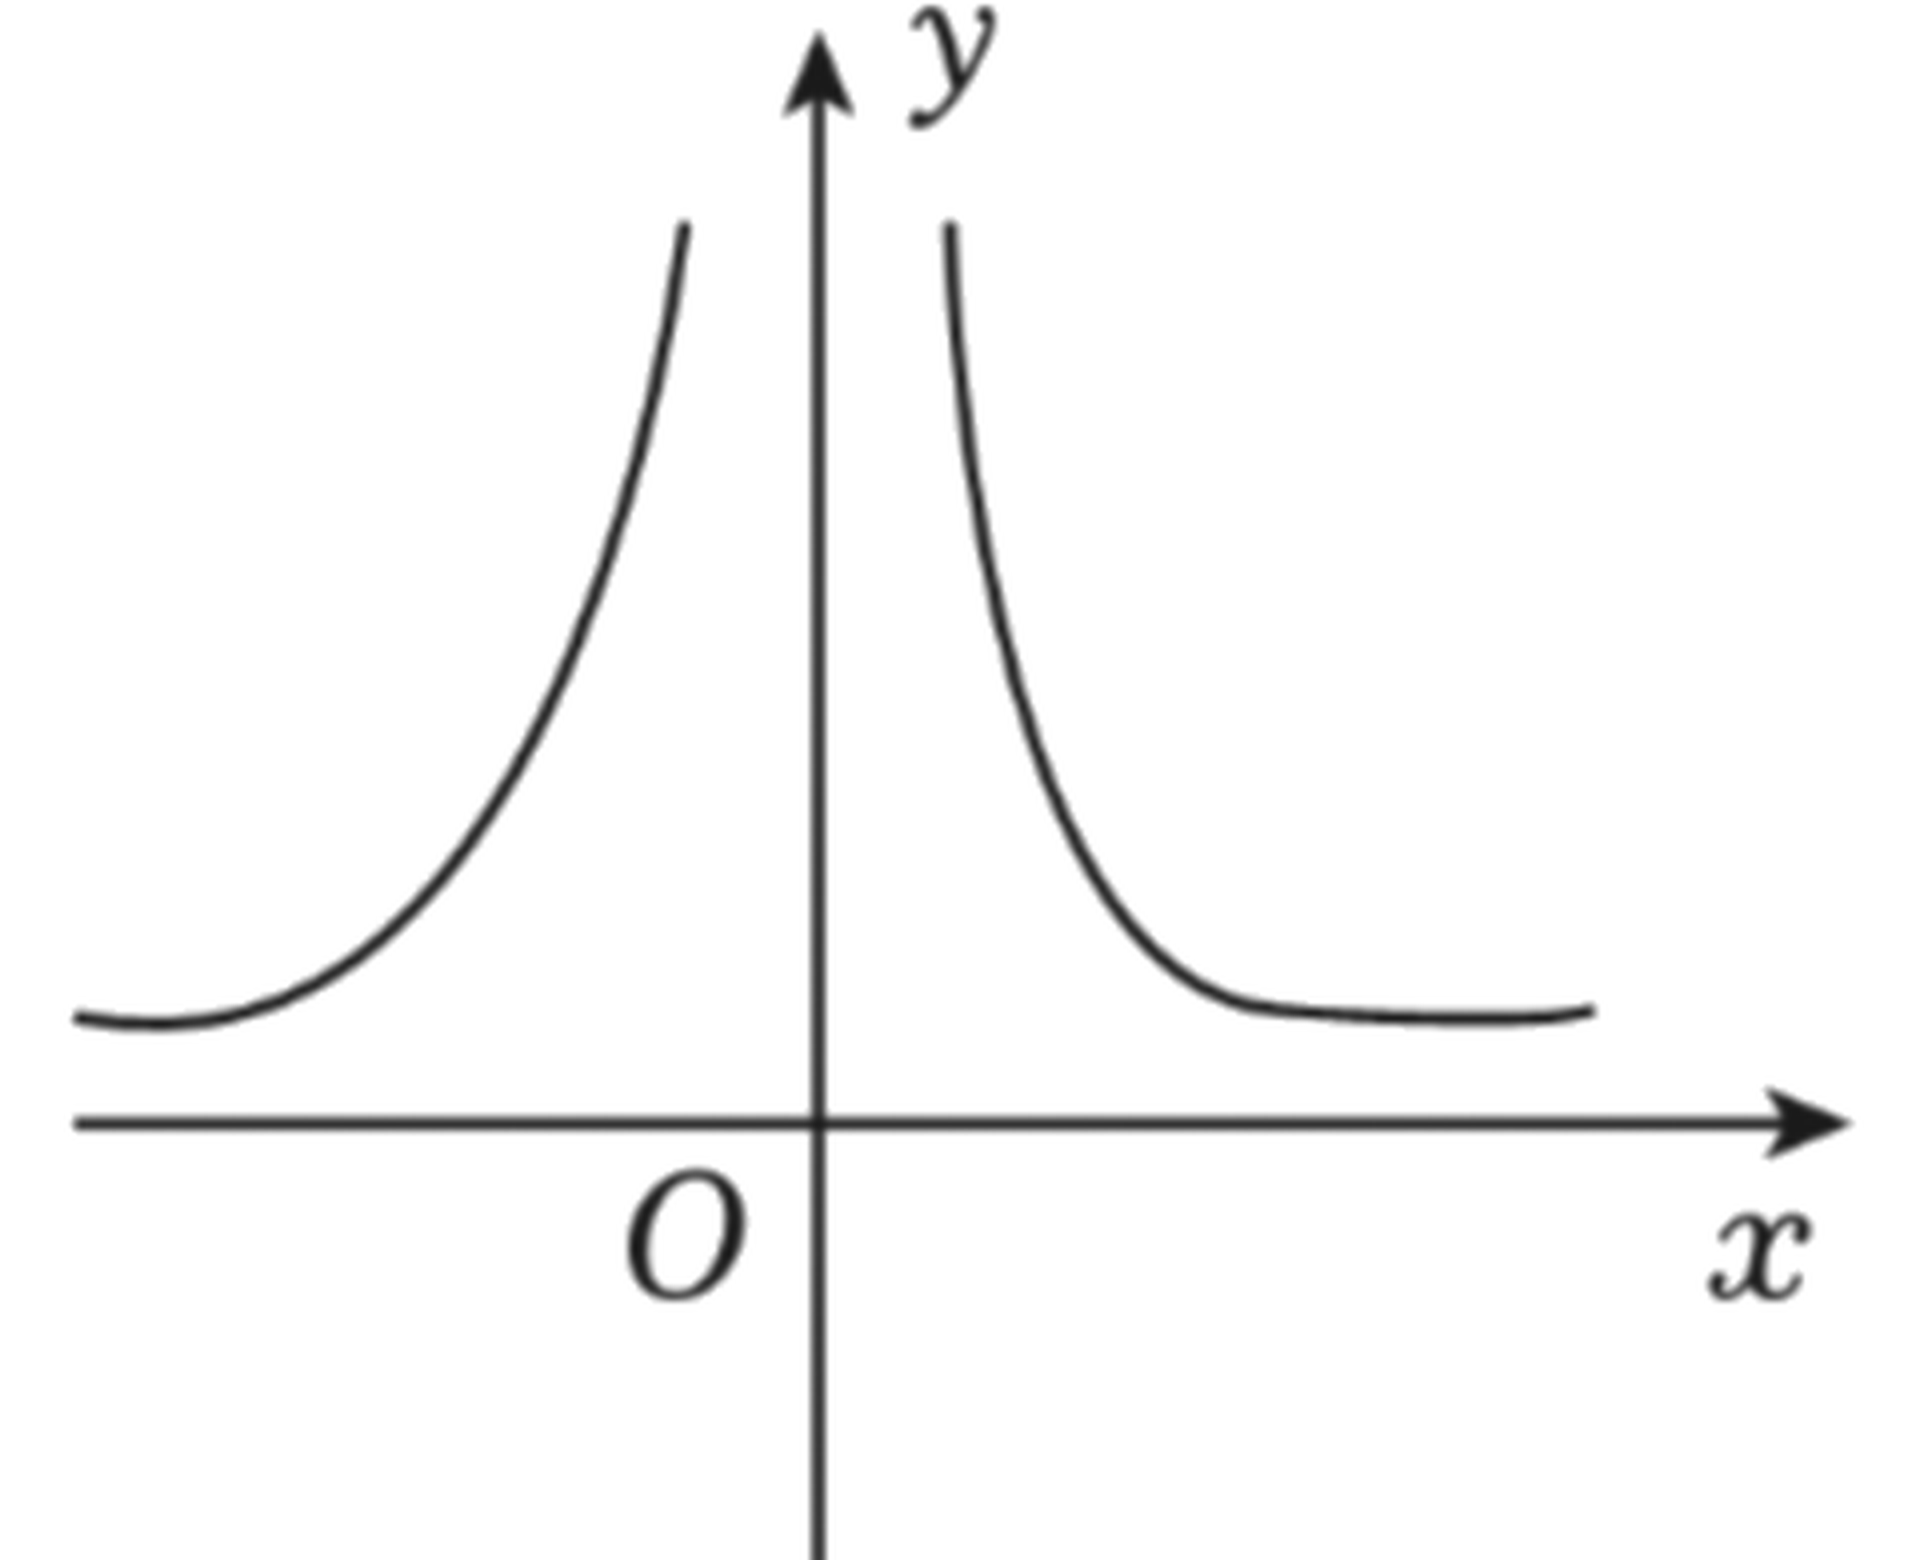
\includegraphics[width=0.36\textwidth]{figures/gao148_q16.png}
\end{center}

\ifanswer
\solbegin
\step{因为函数为偶函数，所以 $p$ 为偶数，且由图象形状判定 $\dfrac{p}{q}<0$.}
\step{又 $p$、$q$ 互质，所以 $q$ 为奇数. 故选 $D$.}
\solend
\fi

\end{enumerate}

\bigsec{三、解答题}

\begin{enumerate}
\setcounter{enumi}{16}

% === Q17 ===：\overline{B}／\varnothing／\R／\mid 逐处照录；解析 8 行
\item 已知集合 $A=\left\{x\mid \dfrac{5}{2x+1}>1\right\}$，$B=\{x\mid x^2+(a+3)x+3a<0,a\in\R\}$.

(1) 求 $A$.

(2) 若全集 $U=\R$，且 $A\cap\overline{B}=\varnothing$，求实数 $a$ 的取值范围.

\ifanswer
\solbegin
\step{(1) $\dfrac{5}{2x+1}>1$，即 $\dfrac{5}{2x+1}-1>0$，即 $\dfrac{4-2x}{2x+1}>0$，即 $(2x+1)(x-2)<0$，}
\step{解得 $-\dfrac{1}{2}<x<2$，所以 $A=\left(-\dfrac{1}{2},2\right)$；}
\step{(2) $x^2+(a+3)x+3a<0$，即 $(x+3)(x+a)<0$，}
\step{全集 $U=\R$，且 $A\cap\overline{B}=\varnothing$，}
\step{当 $a<3$ 时，解得 $-3<x<-a$，则 $\overline{B}=(-\infty,-3)\cup(-a,+\infty)$，}
\step{此时 $-a\geqslant2$，解得 $a\leqslant-2$，}
\step{当 $a\geqslant3$ 时，不满足 $A\cap\overline{B}=\varnothing$，}
\step{故实数 $a$ 的取值范围是 $(-\infty,-2]$.}
\solend
\fi

% === Q18 ===：cases 块整体算一个印刷行；解析 6 行
\item 已知幂函数经过点 $(2,4)$.

(1) 当 $x=\dfrac{1}{2}$ 时，求函数的值；

(2) 是否存在实数 $m$、$n$，使得该函数在区间 $[m,n]$ 上最小值为 $6m-8$，最大值为 $6n-8$？若存在，求出 $m$、$n$ 的值，若不存在，请说明理由.

\ifanswer
\solbegin
\step{(1) 设幂函数的解析式是 $y=x^\alpha$，则 $2^\alpha=4$，解得 $\alpha=2$，}
\step{故 $f(x)=x^2$，$f\left(\dfrac{1}{2}\right)=\dfrac{1}{4}$；}
\step{(2) 因为 $f(x)\geqslant0$，所以 $6m-8\geqslant0$，$m\geqslant\dfrac{4}{3}$，}
\step{由函数 $f(x)$ 在 $(0,+\infty)$ 严格增，得函数 $f(x)$ 在 $(m,n)$ 严格增，}
\step{所以 $\begin{cases}f(m)=6m-8\\f(n)=6n-8\end{cases}$ 且 $m<n$，解得 $m=2$，$n=4$，}
\step{故存在 $m=2$，$n=4$ 满足题意.}
\solend
\fi

% === Q19 ===：7 处评分档照 高一54／64 成例排 \dots\dots N 分；判别式高 \Delta；解析 9 行
\item 已知方程 $x^2+6mx+9m-2=0$，且 $x_1,x_2$ 是方程的两个不同的实数根.

(1) 若 $m=1$，求 $\dfrac{1}{x_1}+\dfrac{1}{x_2}$ 的值；

(2) 若 $m\in\R$，且 $x_1^2+x_2^2<4$，求 $m$ 取值范围.

\ifanswer
\solbegin
\step{(1) 当 $m=1$ 时，方程为 $x^2+6x+7=0$，\dots\dots1 分}
\step{则 $x_1+x_2=-6,x_1\cdot x_2=7$，\dots\dots2 分}
\step{$\dfrac{1}{x_1}+\dfrac{1}{x_2}=\dfrac{x_1+x_2}{x_1\cdot x_2}=-\dfrac{6}{7}$\dots\dots3 分}
\step{(2) $x_1+x_2=-6m,x_1\cdot x_2=9m-2$\dots\dots2 分}
\step{因为 $x_1^2+x_2^2=(x_1+x_2)^2-2x_1\cdot x_2$，所以 $(x_1+x_2)^2-2x_1\cdot x_2<4$，}
\step{所以 $36m^2-2(9m-2)<4$，解得 $0<m<\dfrac{1}{2}$\dots\dots2 分}
\step{又因为方程有两个不同的根，所以 $\Delta=36m^2-4(9m-2)>0$，}% 判别式原卷印等腰偏高粗三角 $\Delta$，照录（放大 07 页 q19_delta3.png／diag_band_q19.png 确认）
\step{解得 $m<\dfrac{1}{3}$ 或 $m>\dfrac{2}{3}$\dots\dots2 分}
\step{所以 $0<m<\dfrac{1}{3}$\dots\dots2 分}
\solend
\fi

% === Q20 ===：题目配图（矩形蔬菜温室，三版都出），\needvspace 守卫放 \item 之前；单位 \mathrm{m}／\mathrm{m}^2；解析 10 行
\needvspace{8cm}
\item 某村计划建造一个室内面积为 $600\mathrm{m}^2$ 的矩形蔬菜温室，在室内，沿左、右两侧与后侧内墙各保留 $2\mathrm{m}$ 宽的通道，沿前侧内墙保留 $4\mathrm{m}$ 宽的空地.

\begin{center}
% 矩形蔬菜温室示意图取 07 页右侧，去粉色水印、去色、4× LANCZOS 放大；三版都出
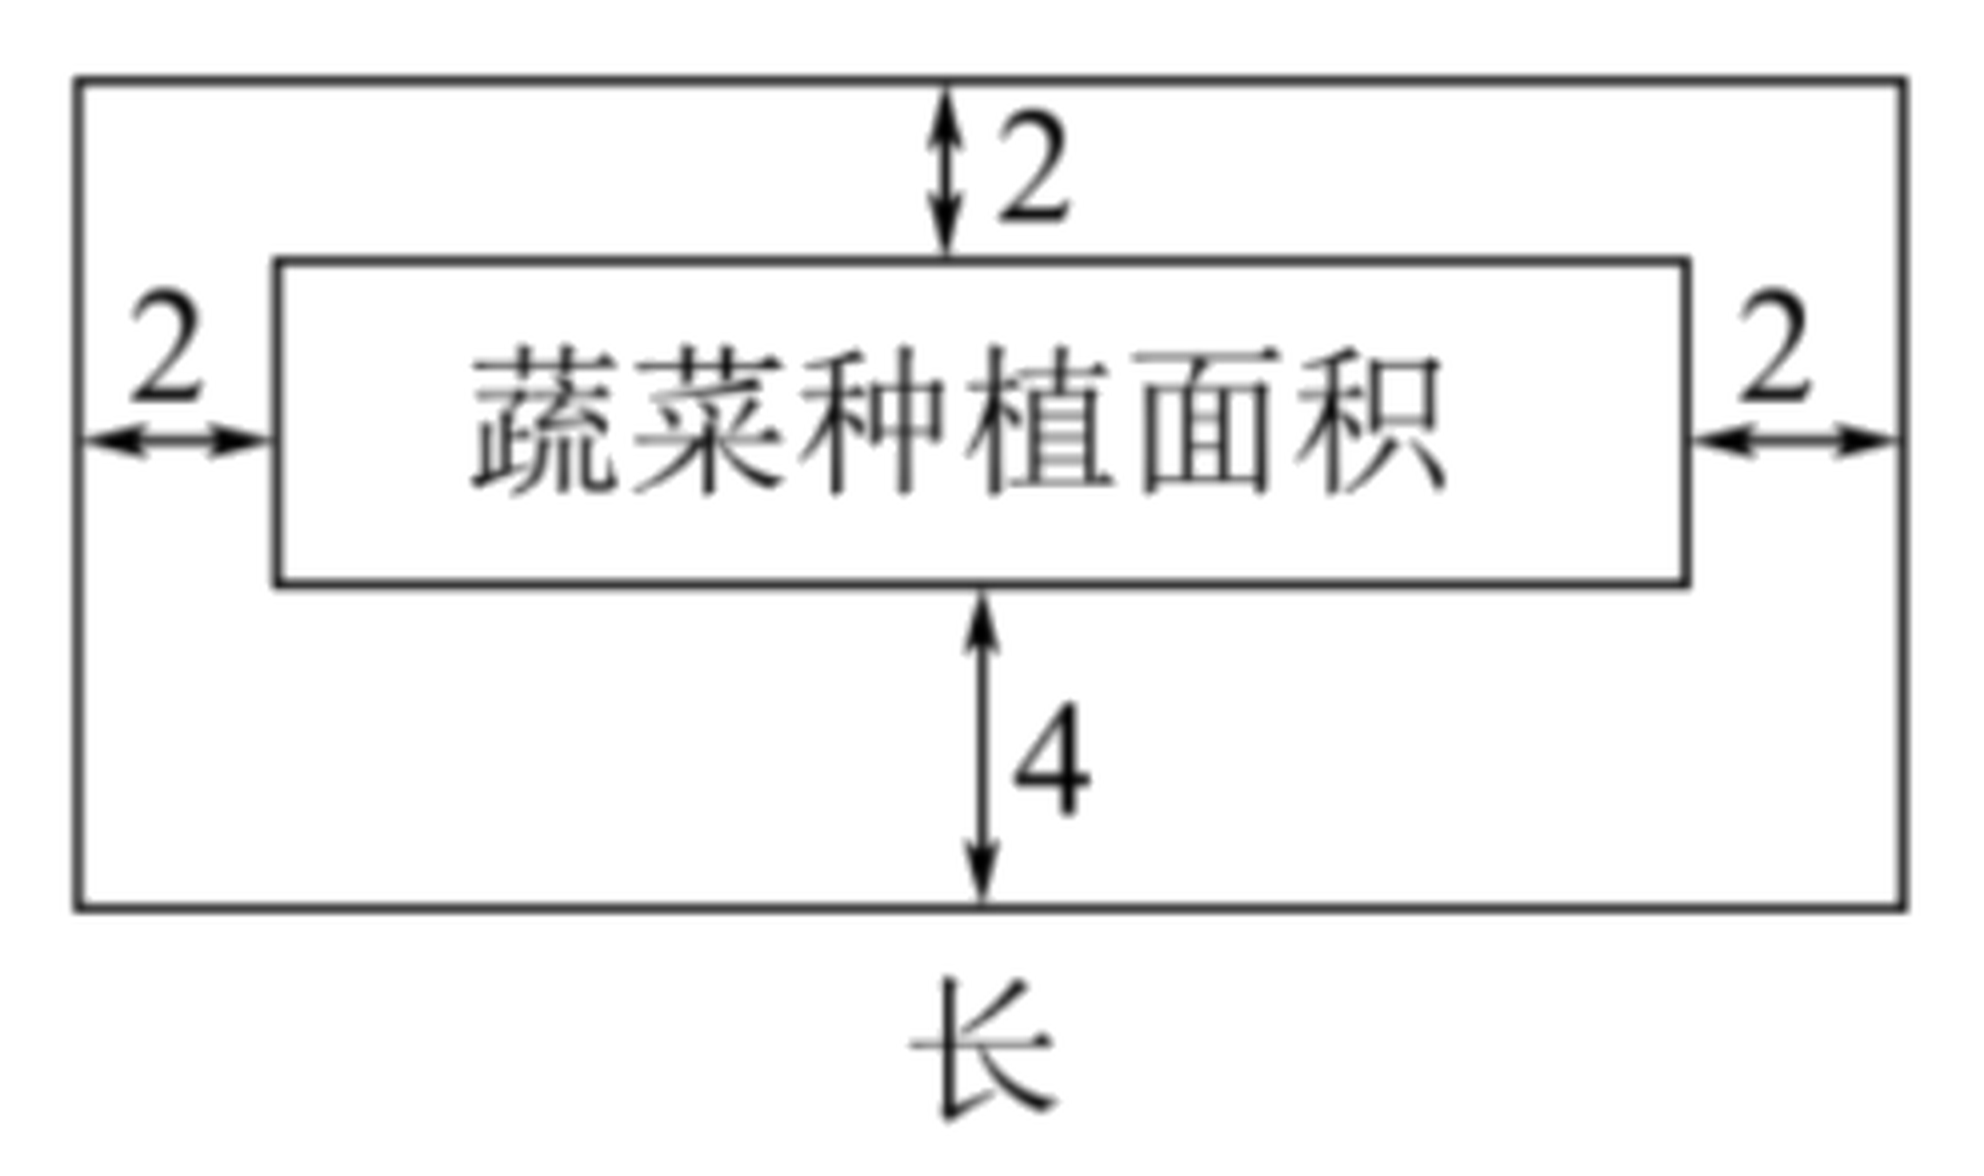
\includegraphics[width=0.45\textwidth]{figures/gao148_q20.png}
\end{center}

(1) 写出蔬菜的种植面积关于矩形温室的长之间的关系式.

(2) 当矩形温室的边长各为多少时，蔬菜的种植面积最大？最大种植面积是多少？

\ifanswer
\solbegin
\step{(1) 设蔬菜的种植面积为 $y\mathrm{m}^2$，矩形温室的长为 $x\mathrm{m}$，}
\step{则矩形温室的宽为 $\dfrac{600}{x}\mathrm{m}$，}
\step{种植蔬菜矩形的长为 $(x-4)\mathrm{m}$，宽为 $\left(\dfrac{600}{x}-6\right)\mathrm{m}$，}
\step{所以 $y=(x-4)\left(\dfrac{600}{x}-6\right)(4<x<100)$；}
\step{(2) 因为 $y=(x-4)\left(\dfrac{600}{x}-6\right)=624-\left(6x+\dfrac{2400}{x}\right)$，}
\step{因为 $6x+\dfrac{2400}{x}\geqslant2\sqrt{6x\cdot\dfrac{2400}{x}}=240$，}
\step{当且仅当 $6x=\dfrac{2400}{x}$，即 $x=20$ 时取等号，}
\step{所以 $y=624-\left(6x+\dfrac{2400}{x}\right)\leqslant624-240=384$.}
\step{即当矩形温室的一边长为 $20\mathrm{m}$，另一边长为 $30\mathrm{m}$ 时，}
\step{蔬菜的种植面积最大，最大为 $384\mathrm{m}^2$.}
\solend
\fi

% === Q21 ===：3 问、cases 块整体算一个印刷行；判别式高 \Delta；解析 19 行（末行续 09 页）
\item 二次函数 $f(x)=ax^2+bx+c$ 满足对任意的 $x\in\R$，$x-1\leqslant f(x)\leqslant x^2-x$ 恒成立.

(1) 求证：$f(1)$ 为定值；

(2) 若 $f(0)=-\dfrac{1}{4}$，求二次函数 $f(x)$ 的表达式；

(3) 求 $a+2b+5c$ 的取值范围.

\ifanswer
\solbegin
\step{(1) 对任意的 $x\in\R$，$x-1\leqslant f(x)\leqslant x^2-x$ 恒成立，则 $0\leqslant f(1)\leqslant0$，}
\step{所以 $f(1)=0$，为定值.}
\step{(2) 由(1)得 $a+b+c=f(1)=0$，由 $f(0)=-\dfrac{1}{4}$，得 $c=-\dfrac{1}{4}$，}
\step{则 $b=\dfrac{1}{4}-a$，$f(x)=ax^2+\left(\dfrac{1}{4}-a\right)x-\dfrac{1}{4}$，}
\step{不等式 $x-1\leqslant f(x)$ 可化为 $ax^2+\left(\dfrac{1}{4}-a\right)x-\dfrac{1}{4}\geqslant x-1$，}
\step{即 $ax^2-\left(a+\dfrac{3}{4}\right)x+\dfrac{3}{4}\geqslant0$，}
\step{一元二次不等式 $ax^2-\left(\dfrac{3}{4}+a\right)x+\dfrac{3}{4}\geqslant0$ 恒成立，则 $\begin{cases}a>0\\\Delta=\left(a+\dfrac{3}{4}\right)^2-3a\leqslant0\end{cases}$，}% 判别式原卷印等腰偏高粗三角 $\Delta$，照录（放大 08 页 q21_delta3.png／diag_band_q21.png 确认）
\step{解得 $a=\dfrac{3}{4}$，}
\step{此时 $f(x)=\dfrac{3}{4}x^2-\dfrac{1}{2}x-\dfrac{1}{4}$，$x^2-x-f(x)=\dfrac{1}{4}(x-1)^2\geqslant0$ 恒成立，}
\step{所以 $f(x)=\dfrac{3}{4}x^2-\dfrac{1}{2}x-\dfrac{1}{4}$.}
\step{(3) 由(1)得 $b=-a-c$，$f(x)=ax^2-(a+c)x+c=(ax-c)(x-1)$，}
\step{不等式 $x-1\leqslant f(x)$ 可化为 $(x-1)(ax-c-1)\geqslant0$，}
\step{一元二次不等式 $(x-1)(ax-c-1)\geqslant0$ 恒成立，则 $a>0$，}
\step{且方程 $(x-1)(ax-c-1)=0$ 有相等的实数根，因此 $c=a-1$，$a>0$，}
\step{不等式 $f(x)\leqslant x^2-x\Leftrightarrow(ax-c)(x-1)\leqslant x^2-x\Leftrightarrow(x-1)[(1-a)x+c]\geqslant0$，}
\step{同理 $1-a>0$，且方程 $(x-1)[(1-a)x+c]=0$ 有相等的实数根，}
\step{因此 $c=a-1$，$a<1$，从而 $c=a-1$，$b=1-2a$，$0<a<1$，}
\step{$a+2b+5c=a+2(1-2a)+5(a-1)=2a-3\in(-3,-1)$，}
\step{所以 $a+2b+5c$ 的取值范围是 $(-3,-1)$.}
\solend
\fi

\end{enumerate}

\end{document}
"
%
% ① 原始材料：微信公众号"魔都数学加油站"文章，连载"27学年高一148"，原文标题
% "27学年高一148——2026-2027年上海市新川中学高一上期中"（2026-11-21 推送）；
% 原文链接：https://mp.weixin.qq.com/s/Alhmwb3sSLQMp_wjzoAVyA 。
% 正文为 9 张 PNG 页（01/03/04/07/08/09 为 2560×3620，02/05/06 为 4762×6735，
% 同一篇各页分辨率混排，逐页按各自分辨率裁图核对，别按预览比例换算裁框）。
% 体例：混合体例讲评版——19 题中 Q4、Q5 只印【答案】、无【解析】；Q13 的答案"C"
% 直接印在题干括号内、无【答案】/【解析】段；其余 16 题印【解析】（逐题核实，见 ② ②）。
% 题目、答案、解析均据原图转录；卷面粉红色水印"魔都数学加油站"及公众号页脚未录入。
% 全卷插图清单（逐页通读 9 页确认）：4 幅题目配图，均三版都出、均非【解析】内配图：
%   · Q12 幂函数曲线族图（03 页右侧：x/y 轴、O、A(1,0)、B(0,1)、M、N 与两族
%     y=x^α／y=x^β 曲线、线段 AB、虚线），题干"（如图）"处，裁 figures/gao148_q12.png；
%   · Q15 四条指数函数曲线图（04 页右侧：①②③④ 四曲线同过 (0,1)、x/y 轴、O、
%     y 轴刻度 1），题干"如图"处，裁 figures/gao148_q15.png；
%   · Q16 关于 y 轴对称的幂函数曲线图（04 页右下：x/y 轴、O、两支上翘曲线），
%     题干"如图所示"处，裁 figures/gao148_q16.png；
%   · Q20 矩形蔬菜温室示意图（07 页右侧：大矩形＋内框"蔬菜种植面积"＋2/2/4
%     通道标注＋"长"），题干处，裁 figures/gao148_q20.png；
%   其余各页逐页确认无其它题目配图、无【解析】内配图、无表格，亦无"题干写如图而
%   源码漏图"一处；Q19 解析行末的虚线"----N 分"为评分档（非图），Q18／Q21 的
%   cases 块为数学块（非图）。4 图均取自原卷截图，去粉色水印、去色、4× LANCZOS 放大。
%
% 卷首标题：原卷印作"2026-2027 年新川中学高一上期中"，年份区间按全稿惯例排 en dash；
% 原卷卷面未印副标题，本稿按同期中卷（高一140／141／143／144／145／146／147）知识模块
% 口径补出"集合与常用逻辑用语、不等式、函数"。
%
% 题号体例（逐页核实定稿）：本卷共 19 题——一、填空题 3—12（10 题）、
% 二、选择题 13—16（4 题）、三、解答题 17—21（5 题）。
% 三节分别 \setcounter{enumi}{2}／{12}／{16}。原卷从第 3 题起、无第 1、2 题，
% 本稿保留原题号；全卷无附加题节、无 Q22（Q21 解析末行"所以 a+2b+5c 的取值范围是
% (-3,-1)."为全卷收尾，09 页下半仅水印、无正文）。
%
% ② 与原卷的排版差异：
%   ① 原文从第 3 题起，本稿保留原题号；共 19 题三节；
%   ② 混合体例逐题核实：Q4（反证法"假设的内容"）、Q5 只印【答案】、无【解析】，
%      按 高一140 第 5 题／高一145 Q3 成例提 \ans{}、不补造解析；Q13 答案"C"直接
%      印在题干括号内（" ( C ) "）、全卷无该题【答案】/【解析】段，按 高一84 Q13／
%      高一37 Q13／高一53 Q13 成例括号 \mbox{（\quad）} 留空、另提 \ans{$C$}；
%      其余 16 题印【解析】、用 \solbegin…\solend，选择题答案在解析末句"故选 X"
%      （Q14 选 D、Q15 选 B、Q16 选 D，逐个放大原图核实）、题干括号留空、不另提
%      \ans{}；答案版【答案】/【解析】标记数 = 19（3 个 \ans ＋ 16 个 \solbegin）
%      = 全卷题数；
%   ③ 原卷卷面未印副标题，本稿按知识模块口径补出；
%   ④ 原卷填空横线按全稿惯例排 \blankline[4.4em]；选择题括号排 \mbox{（\quad）}、
%      选项段前按惯例加 \keepwithprev；Q13／Q16 四选项为两行两列、Q14／Q15 选项
%      为一行，照原卷分行；解答题不留作答区、不加 \anspace（原卷为讲评版，
%      与 129／131／132／133／136／140／141／143／144／145／146 同）；
%   ⑤ 数集：Q11"在 R 上定义运算"、Q13"x、y∈R"、Q16"p、q∈Z"、Q17"a∈R"
%      "U=R"、Q19"m∈R"、Q21"x∈R" 原卷印斜体 R/Z，按全稿惯例统一改 \R／\Z
%      （本卷未出现 N，\N^* 无对应处）；绝对值排 \lvert…\rvert（Q9／Q14），
%      集合描述竖线排 \mid（Q17）；不等号按全稿惯例排 \leqslant／\geqslant；
%      补集照原卷上划线排 \overline{B}（Q17 题干 1 处＋解析 3 处）；空集
%      \varnothing（Q17 题干 1 处＋解析 2 处）；\subset（Q3 题干 {a}⊂M）与
%      \subseteq（Q3 题干 M⊆{a,b,c,d}）逐处照录不统一（放大 01 页 q3_subset.png）；
%   ⑥ 子题标号 (1)(2)(3) 半角括号照录；圈数字 ①—⑥ 在文本模式（Q14 六个结论、
%      Q15 曲线编号与其解析、Q14 解析"对①…对⑥"），按 common.sty 划入 CJK 字符类
%      渲染；cases 块整体算一个印刷行；\left…\right 不得拆到不同 $…$ 组；
%      单位 m／m² 排 \mathrm{m}／\mathrm{m}^2（Q20，原卷印正体 m）；
%   ⑦ 题干／解析中的中文弯引号按原卷照录：Q4" ab 可以被 5 整除，那么 a、b 中
%      至少有一个能被 5 整除 "（开引号后有空格、闭引号后空格接"时"）、
%      Q13" x=0 "" xy=0 "（引号内空格），注释内一律 ASCII 引号；
%   ⑧ 半角逗号在数学组之间是全稿惯例、非笔误（Q3"{a,b,c,d}"、Q6"$x,y$"
%      "$x=\frac13,y=\frac16$"、Q10、Q11"$a=-2,b=-1"、Q12"$\alpha=\log..,\beta=..$"、
%      Q14"$a+b<0,a-b<0$"、Q17、Q19"$x_1+x_2=-6,x_1\cdot x_2=7$"、Q20、Q21 等），
%      逐处照录别改全角；行末西文句点照录为 ASCII `.`；行中全角逗号／顿号照录；
%   ⑨ "图像／图象"逐处放大核：全卷 9 处均印"图象"（象，无亻）、未见"图像"，
%      逐处照录未统一改动（Q8 题干/解析各 1、Q12 题干 2、Q15 题干 1／解析 2、
%      Q16 题干 1／解析 1；放大 02/03/04/05 页 /tmp/gao148/zoom/my_wide_a.png、
%      my_wide_b.png 与宋体参考"象／像"并排确认）；
%   ⑩ 判别式 Δ/△ 混用是照录项：Q11 解析"△=1−4(−a²+a+1)<0"印扁等边空心
%      三角 \triangle；Q19 解析"Δ=36m²−4(9m−2)>0"、Q21 解析 cases 块
%      "Δ=(a+3/4)²−3a≤0" 两处印等腰偏高粗三角 \Delta，逐处放大判断、照录
%      不统一（参照 高一142／144／145 头注④口径，详见 ④）；
%   ⑪ 一条 \step = 原卷解析的一个印刷行，cases 块整体算一个印刷行；别把原卷折行
%      并起来、别把一行拆多条。Q3 六行、Q7 五行（01 页末首行＋02 页顶四行）、
%      Q9 七行、Q11 五行、Q14 八行（对② 的两行公式各占一印刷行）、Q17 八行、
%      Q18 六行、Q19 九行（7 处评分档附在行末）、Q20 十行、Q21 十九行
%      均按印刷行逐条断，不丢行；
%   ⑫ 配图：4 幅均为题目配图（三版都出），放 \item 内题干之后 \begin{center}；
%      大图块加 \needvspace 守卫把整块推走（守卫放 \item 之前，见 高一145 Q14/Q20
%      成例与切页审计 B 类坑）；三版切页审计均"合计异常：无"；
%   ⑬ 跨页续印按题合并：Q3/4/5 在 01 页；Q6 题干＋解析在 01 页；Q7 题干在 01 页
%      末、解析首行在 01 页末续 02 页顶四行；Q8/9/10 在 02 页（Q9 解析续 02 页下半、
%      Q10 题干与解析前 2 行在 02 页末）；Q10 解析末行续 03 页顶；Q11/12 在 03 页、
%      "二、选择题"标题与 Q13/14 题干在 03 页下半；Q13 无解析；Q14 解析在 04 页顶、
%      Q15 题干＋图＋选项＋解析在 04 页、Q16 题干＋图在 04 页末；Q16 选项＋解析＋
%      "三、解答题"标题＋Q17 题干＋解析在 05 页、Q18 题干首句在 05 页末；Q18 题干
%      续＋解析、Q19 题干＋解析前 5 行在 06 页；Q19 解析续 4 行＋Q20 题干＋图＋
%      解析（10 行全部）在 07 页，末行"蔬菜的种植面积最大，最大为 384m²."收尾；
%      Q21 题干＋解析前 18 行在 08 页；Q21 解析末行"所以 a+2b+5c 的取值范围是
%      (-3,-1)."在 09 页上半（09 页下半仅水印、无正文）。本稿按题连排，不丢行、
%      不并折行；
%   ⑭ 原卷解析内无红色"法一／法二"之类小标题，故本卷无 \stepm；水印
%      "魔都数学加油站"红色不录入；Q19 解析 7 处评分档（1/2/3/2/2/2/2 分）
%      原卷在行末印一串虚线，本稿照 高一54／64 成例排 \dots\dots N 分，
%      分值逐处照录、位置不变。
%
% ③ 行数复核：一条 \step／\stepm = 原卷解析的一个印刷行，cases 块作一个印刷行计。
%   逐题数（主会话逐页核对定稿）：Q3：6；Q4：0（只印【答案】、提 \ans{}）；
%   Q5：0（只印【答案】、提 \ans{}）；Q6：2；Q7：5；Q8：2；Q9：7；Q10：3；
%   Q11：5；Q12：2；Q13：0（答案印在题干括号内、另提 \ans{}）；Q14：8；Q15：5；
%   Q16：2；Q17：8；Q18：6；Q19：9；Q20：10；Q21：19。
%   合计 99 条 \step（本卷无 \stepm：解析内无红色"法一／法二"类小标题），
%   与原卷逐题印刷行相等。全卷 16 题设 \solbegin…\solend ＋ 3 处 \ans{}，
%   答案版【答案】/【解析】标记数 = 19 = 全卷题数。
%
% ④ 判别式／子集符号结论（逐处放大原图照录、不得统一，主会话像素级复核）：
%   判别式全卷 3 处，两形混用逐处照录不统一（参照 高一142／144／145 头注④口径）：
%     · Q11 解析"△=1−4(−a²+a+1)<0" 原卷印扁等边空心三角（宽>高、细线），
%       照录 \triangle（放大 03 页 /tmp/gao148/zoom/q11_delta3.png、
%       delta_montage.png 确认）；
%     · Q19 解析"Δ=36m²−4(9m−2)>0" 原卷印等腰偏高粗三角（高>宽），
%       照录 \Delta（放大 07 页 /tmp/gao148/zoom/q19_delta3.png 确认）；
%     · Q21 解析 cases 块"Δ=(a+3/4)²−3a≤0" 原卷印等腰偏高粗三角（高>宽），
%       照录 \Delta（放大 08 页 /tmp/gao148/zoom/q21_delta3.png 确认）。
%   子集／补集：Q3 题干"{a}⊂M⊆{a,b,c,d}" 前者印单线 ⊂、无下划线，照录 \subset；
%     后者印带下划线 ⊆，照录 \subseteq（放大 01 页 /tmp/gao148/zoom/q3_subset.png
%     确认）；Q17 题干 1 处＋解析 3 处共 4 处 \overline{B} 照原卷上划线
%     （B 上横线、非 C_U B）；空集 \varnothing 3 处（Q17 题干 1 处、解析 2 处）；
%     Q17 集合描述竖线 \mid；数集 \R／\Z 归一见 ② ⑤。
%
% ⑤ 存疑照录（放大原图确认，照录未改、正文对应处另有 % 注）：
%   1. Q3 解析末行"所以 M 一共有 3+3+1+1=8 个" 原卷印 $3+3+1+1=8$，按上文
%      四行应为 $1+3+3+1=8$（疑为原卷加数顺序笔误，和仍为 8），放大 01 页
%      /tmp/gao148/zoom/my_q3_sol.png 确认，照录未改。
%   2. Q13 答案"C"直接印在题干括号内、全卷无该题【答案】/【解析】段，按
%      高一84 Q13 成例括号留空、另提 \ans{$C$}（见 ② ②），未补造解析。
%   3. Q19 解析 7 处评分档（"----N 分"）原卷印一串虚线，本稿照 高一54／64
%      成例排 \dots\dots N 分，分值逐处照录、位置不变。
%   4. 判别式 Q11 扁 \triangle 与 Q19／Q21 高 \Delta 两形混用，逐处照录不统一（见 ④）。
%   5. "图像／图象"全卷 9 处均印"图象"、未见"图像"（见 ② ⑨），逐处放大核实照录，
%      未统一改动。
%   全卷除此 5 类外未发现其它笔误／自相矛盾处。
%
% ⑥ 跨页续印按题合并说明：见 ② ⑬。
%
\documentclass[a4paper,11pt]{article}
\usepackage{common}

\begin{document}

\examtitlest[3]{2026--2027 年新川中学高一上期中}{集合与常用逻辑用语、不等式、函数}

\bigsec{一、填空题}

\begin{enumerate}
\setcounter{enumi}{2}

% === Q3 ===：题干 {a}⊂M⊆{a,b,c,d} 两个子集符号逐处照录；解析 6 行
\item 满足 $\{a\}\subset M\subseteq\{a,b,c,d\}$ 的集合 $M$ 有\blankline[4.4em]个.

\ifanswer
\solbegin
\step{$M$ 是 $\{a,b,c,d\}$ 的子集，但必含有元素 $a$，}
\step{当 $M$ 中只一个元素时，$M=\{a\}$ 只有 1 个；}
\step{当 $M$ 中有二个元素时，$M$ 有 3 个；}
\step{当 $M$ 中有三个元素时，$M$ 有 3 个；}
\step{当 $M$ 中有四个元素时，$M$ 有 1 个；}
\step{所以 $M$ 一共有 $3+3+1+1=8$ 个.}% 原卷印 $3+3+1+1=8$（按上文四行应为 $1+3+3+1$），疑为加数顺序笔误，照录未改（放大 01 页 my_q3_sol.png）
\solend
\fi

% === Q4 ===：原卷只印【答案】、无【解析】，按 高一140 第 5 题成例提 \ans{}；弯引号与空格照录
\item 用反证法证明命题 “ $ab$ 可以被 5 整除，那么 $a$、$b$ 中至少有一个能被 5 整除” 时假设的内容应该是\blankline[4.4em].

\ifanswer
\ans{$a$、$b$ 都不能被 5 整除}
\fi

% === Q5 ===：原卷只印【答案】 $[-2,1)$、无【解析】，提 \ans{}
\item 不等式 $\dfrac{x+2}{x-1}\leqslant0$ 的解集为\blankline[4.4em].

\ifanswer
\ans{$[-2,1)$}
\fi

% === Q6 ===：解析 2 行；半角逗号在数学组之间照录
\item 设 $x,y\in(0,+\infty)$，且 $x+4y=1$，则 $\dfrac{1}{x}+\dfrac{1}{y}$ 的最小值为\blankline[4.4em].

\ifanswer
\solbegin
\step{因为 $\dfrac{1}{x}+\dfrac{1}{y}=(x+4y)\left(\dfrac{1}{x}+\dfrac{1}{y}\right)=5+\dfrac{4y}{x}+\dfrac{x}{y}\geqslant5+2\sqrt{\dfrac{4y}{x}\cdot\dfrac{x}{y}}=9$，}
\step{当且仅当 $\dfrac{4y}{x}=\dfrac{x}{y}$，即 $x=2y$，即 $x=\dfrac{1}{3},y=\dfrac{1}{6}$ 时取等号，故最小值为 9.}
\solend
\fi

% === Q7 ===：题干在 01 页末、解析首行在 01 页末续 02 页顶四行；解析 5 行
\item 若不等式 $x^2+ax+b<0$ 的解集为 $(-3,-1)$，则不等式 $bx^2+ax+1\leqslant0$ 的解集为\blankline[4.4em].

\ifanswer
\solbegin
\step{不等式 $x^2+ax+b<0$ 的解集为 $(-3,-1)$，}
\step{所以方程 $x^2+ax+b=0$ 的两个实数根为 $-3$ 和 $-1$，}
\step{由根与系数的关系得 $a=4$，$b=3$，}
\step{故 $bx^2+ax+1\leqslant0$ 可化为 $3x^2+4x+1\leqslant0$，解得 $-1\leqslant x\leqslant-\dfrac{1}{3}$，}
\step{所求不等式 $bx^2+ax+1\leqslant0$ 的解集为 $\left[-1,-\dfrac{1}{3}\right]$.}
\solend
\fi

% === Q8 ===："图象"照录；解析 2 行
\item 函数 $y=a^{x-2}+2(a>0,a\ne1)$ 的图象必经过定点\blankline[4.4em].

\ifanswer
\solbegin
\step{令 $x-2=0$，得 $x=2$，则 $y=a^0+2=3$，}
\step{所以函数 $y=a^{x-2}+2$ 的图象过定点 $(2,3)$.}
\solend
\fi

% === Q9 ===：解析 7 行；首句末西文句点照录
\item 不等式 $\lvert x+3\rvert+\lvert a-x\rvert>6$ 对一切实数 $x$ 恒成立，则实数 $a$ 的取值范围为\blankline[4.4em].

\ifanswer
\solbegin
\step{$\lvert x+3\rvert$ 表示 $x$ 到 $-3$ 的距离，$\lvert a-x\rvert$ 表示 $x$ 到 $a$ 的距离.}
\step{所以它们的和为 $x$ 到 $-3$ 和 $x$ 到 $a$ 的距离之和，}
\step{当 $x$ 位于 $-3$ 和 $a$ 之间时，距离和取得最小值，}
\step{即两点之间的距离 $\lvert a-(-3)\rvert=\lvert a+3\rvert$，}
\step{若最小值 $\lvert a+3\rvert>6$，则原式对所有 $x$ 恒成立.}
\step{解得 $a+3>6$ 或 $a+3<-6$，即 $a>3$ 或 $a<-9$，}
\step{故 $a\in(3,+\infty)$ 或 $a\in(-\infty,-9)$.}
\solend
\fi

% === Q10 ===：题干与解析前 2 行在 02 页末、解析末行续 03 页顶；解析 3 行
\item 已知 $2^a=3$，$\log_3 5=b$，则 $\log_{15}20=$\blankline[4.4em]（用 $a$、$b$ 表示）.

\ifanswer
\solbegin
\step{因为 $2^a=3$，所以 $a=\log_2 3=\dfrac{\lg3}{\lg2}$，又 $\log_3 5=b=\dfrac{\lg5}{\lg3}$，}
\step{所以 $\lg3=a\lg2$，$\lg5=b\lg3=ba\lg2$，}
\step{则 $\log_{15}20=\dfrac{2\lg2+\lg5}{\lg3+\lg5}=\dfrac{2\lg2+ab\lg2}{a\lg2+ab\lg2}=\dfrac{2+ab}{a+ab}$.}
\solend
\fi

% === Q11 ===：在 \R 上定义运算 \otimes；判别式扁 \triangle 照录；解析 5 行
\item 在 $\R$ 上定义运算 $\otimes:x\otimes y=x(1-y)$，若不等式 $(x-a)\otimes(x+a)<1$ 对任意实数 $x$ 恒成立，则 $a$ 的取值范围是\blankline[4.4em].

\ifanswer
\solbegin
\step{由题意得不等式 $(x-a)\otimes(x+a)<1$ 对任意实数 $x$ 恒成立，}
\step{即不等式 $(x-a)(1-x-a)<1$ 对任意实数 $x$ 恒成立，}
\step{即 $x^2-x-a^2+a+1>0$ 对任意实数 $x$ 恒成立，}
\step{所以 $\triangle=1-4(-a^2+a+1)<0$，解得 $-\dfrac{1}{2}<a<\dfrac{3}{2}$，}% 判别式原卷印扁等边空心三角 $\triangle$，照录（放大 03 页 q11_delta3.png 确认）
\step{所以实数 $a$ 的取值范围为 $\left(-\dfrac{1}{2},\dfrac{3}{2}\right)$.}
\solend
\fi

% === Q12 ===：题目配图（幂函数曲线族，三版都出）；"图象"照录；解析 2 行
\needvspace{8cm}
\item 幂函数 $y=x^\alpha$，当 $\alpha$ 取不同的正数时，在区间 $[0,1]$ 上它们的图象是一族美丽的曲线（如图）. 设点 $A(1,0)$，$B(0,1)$，连接 $AB$，线段 $AB$ 恰好被其中的两个幂函数 $y=x^\alpha$，$y=x^\beta$ 的图象三等分，即有 $BM=MN=NA$，那么 $\alpha\beta=$\blankline[4.4em].

\begin{center}
% 幂函数曲线族图取 03 页右侧，去粉色水印、去色、4× LANCZOS 放大；三版都出
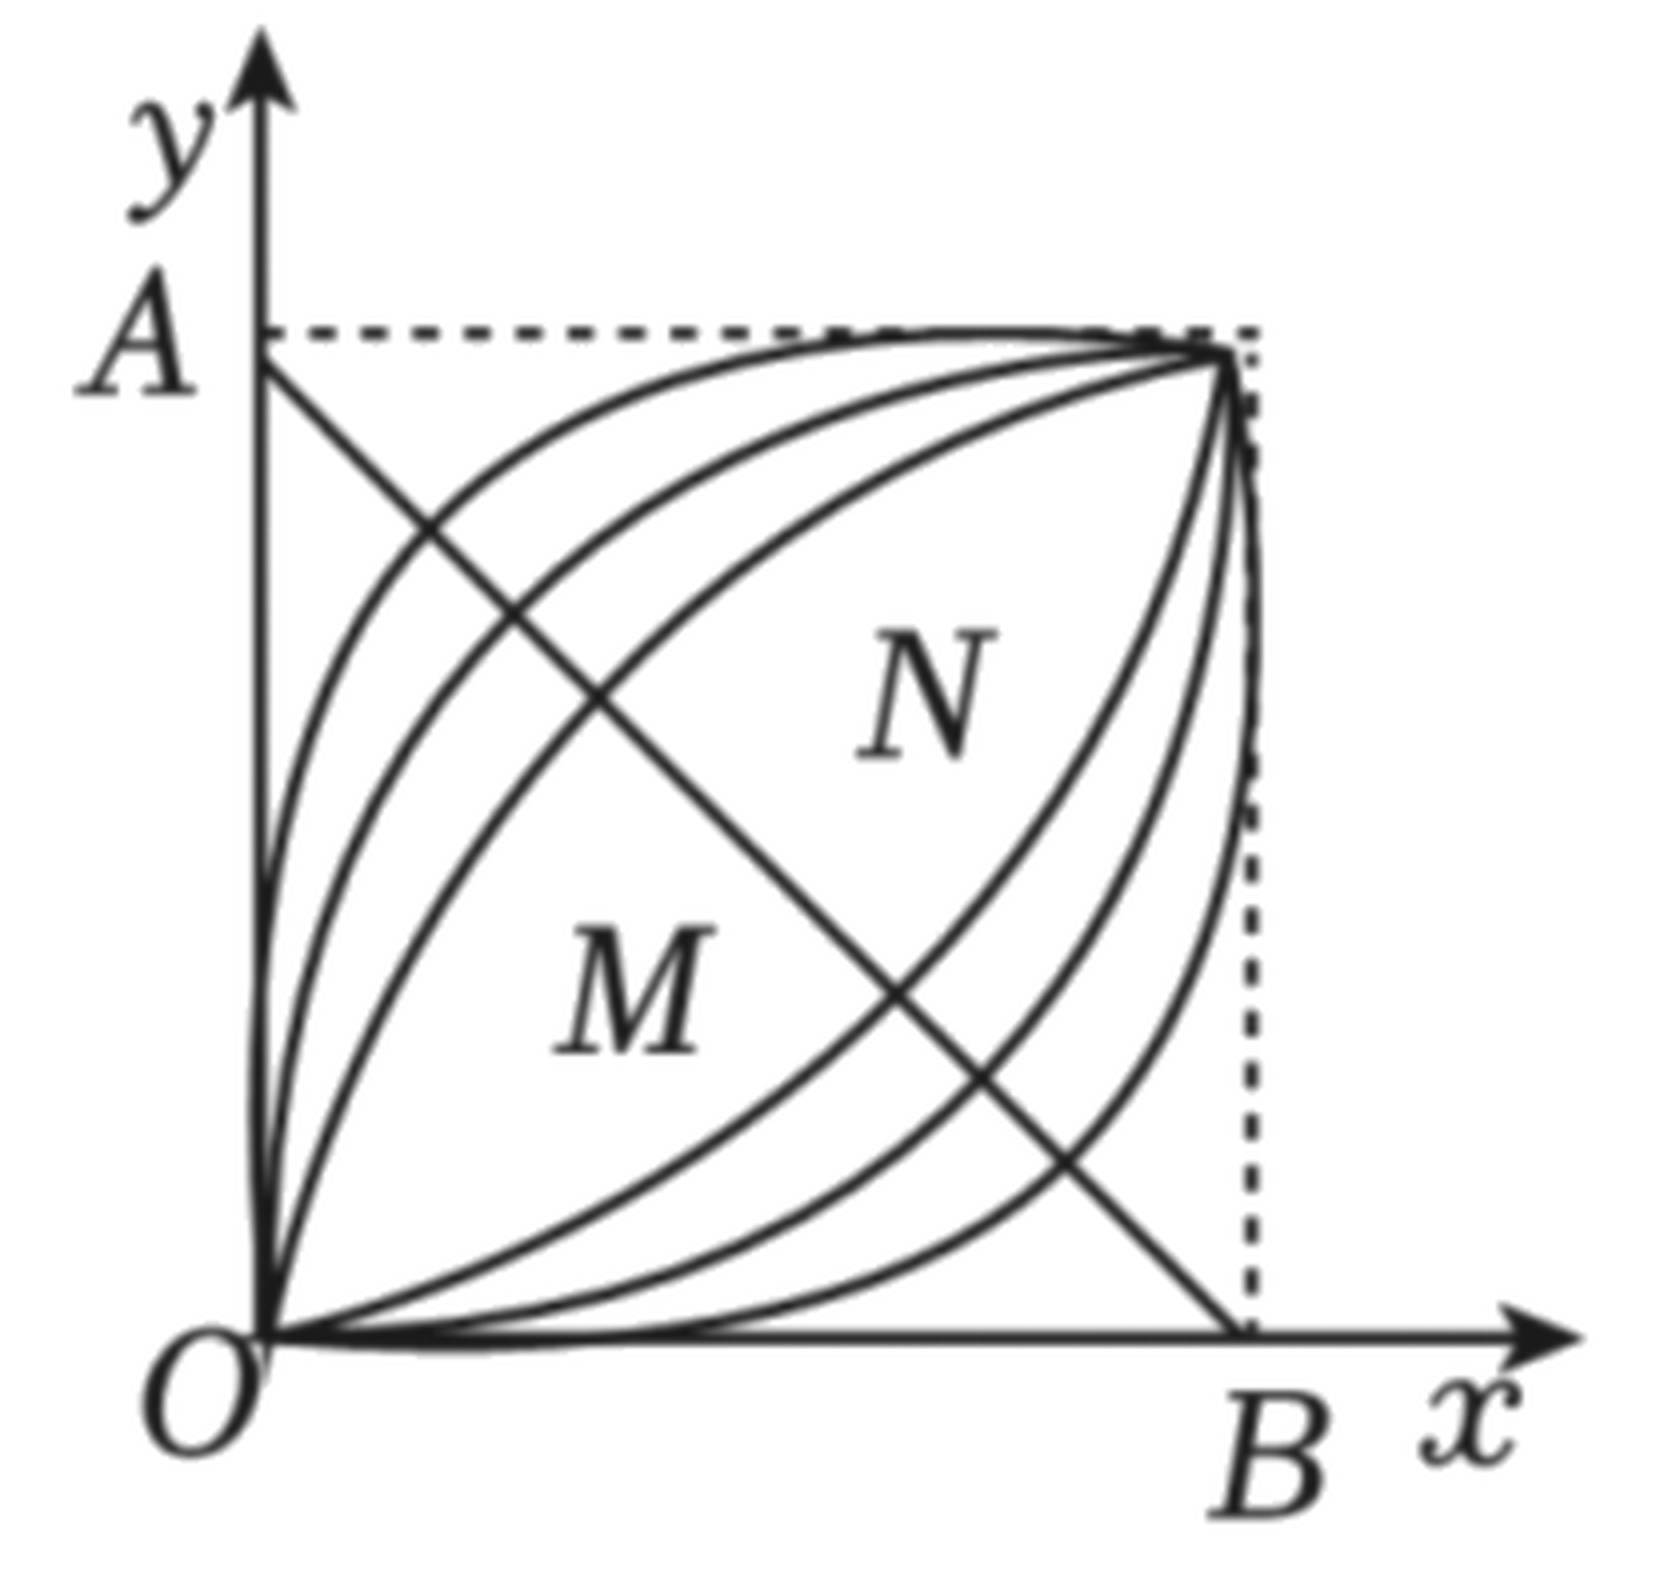
\includegraphics[width=0.40\textwidth]{figures/gao148_q12.png}
\end{center}

\ifanswer
\solbegin
\step{$BM=MN=NA$，点 $A(1,0)$，$B(0,1)$，所以 $M\left(\dfrac{1}{3},\dfrac{2}{3}\right)$，$N\left(\dfrac{2}{3},\dfrac{1}{3}\right)$，}
\step{分别代入 $y=x^\alpha$，$y=x^\beta$，$\alpha=\log_{\frac{2}{3}}\dfrac{1}{3},\beta=\log_{\frac{1}{3}}\dfrac{2}{3}$，$\alpha\beta=\log_{\frac{1}{3}}\dfrac{2}{3}\cdot\log_{\frac{2}{3}}\dfrac{1}{3}=1$.}
\solend
\fi

\end{enumerate}

\bigsec{二、选择题}

\begin{enumerate}
\setcounter{enumi}{12}

% === Q13 ===：答案"C"直接印在题干括号内、全卷无该题【答案】/【解析】段，按 高一84 Q13 成例括号留空、另提 \ans{$C$}；弯引号含空格
\item 若 $x$、$y\in\R$，则 “ $x=0$ ” 是 “ $xy=0$ ” 的\mbox{（\quad）}

\keepwithprev
A. 充要条件\qquad\qquad B. 必要不充分条件

C. 充分不必要条件\qquad\qquad D. 既不充分也不必要条件

\ifanswer
\ans{$C$}
\fi

% === Q14 ===：六个结论（圈数字在文本模式）、四选项一行；解析 8 行（对② 的两行公式各占一印刷行）
\item 若 $a<b<0$，下面有六个结论：① $a^2>b^2$；② $a^3<b^3$；③ $\dfrac{1}{a}<\dfrac{1}{b}$；④ $\dfrac{a}{b}>1$；⑤ $\dfrac{1}{a-b}>\dfrac{1}{a}$；⑥ $\lvert a\rvert>-b$. 其中正确的个数是\mbox{（\quad）}

\keepwithprev
A. 1\qquad\qquad B. 2\qquad\qquad C. 3\qquad\qquad D. 4

\ifanswer
\solbegin
\step{对①：$a^2-b^2=(a+b)(a-b),a+b<0,a-b<0$，故 $a^2-b^2>0$，正确；}
\step{对②：$a^3-b^3=(a-b)(a^2+ab+b^2)=(a-b)\left[\left(a+\dfrac{1}{2}b\right)^2+\dfrac{3}{4}b^2\right],a-b<0$，}
\step{$\left(a+\dfrac{1}{2}b\right)^2+\dfrac{3}{4}b^2>0$，故 $a^3-b^3<0$，正确；}
\step{对③：取 $a=-2,b=-1$，则 $\dfrac{1}{a}=-\dfrac{1}{2},\dfrac{1}{b}=-1,\dfrac{1}{a}>\dfrac{1}{b}$，错误；}
\step{对④：$\dfrac{a}{b}-1=\dfrac{a-b}{b},a-b<0,b<0$，故 $\dfrac{a}{b}-1>0$，正确；}
\step{对⑤：取 $a=-2,b=-1$，则 $\dfrac{1}{a-b}=-1,\dfrac{1}{a}=-\dfrac{1}{2},\dfrac{1}{a-b}<\dfrac{1}{a}$，错误；}
\step{对⑥：要证 $\lvert a\rvert>-b$，即 $-a>-b$，即 $a<b$，正确；}
\step{故选 $D$.}
\solend
\fi

% === Q15 ===：题目配图（四条指数函数曲线，三版都出），\needvspace 守卫放 \item 之前；"图象"照录；解析 5 行
\needvspace{8cm}
\item 如图，曲线①②③④分别是指数函数 $y=a^x$，$y=b^x$，$y=c^x$，$y=d^x$ 的图象，则实数 $a$、$b$、$c$、$d$ 的大小关系为\mbox{（\quad）}

\keepwithprev
A. $a<b<c<d$\qquad B. $b<a<d<c$\qquad C. $d<c<b<a$\qquad D. $c<d<a<b$

\begin{center}
% 四条指数函数曲线图取 04 页右侧，去粉色水印、去色、4× LANCZOS 放大；三版都出
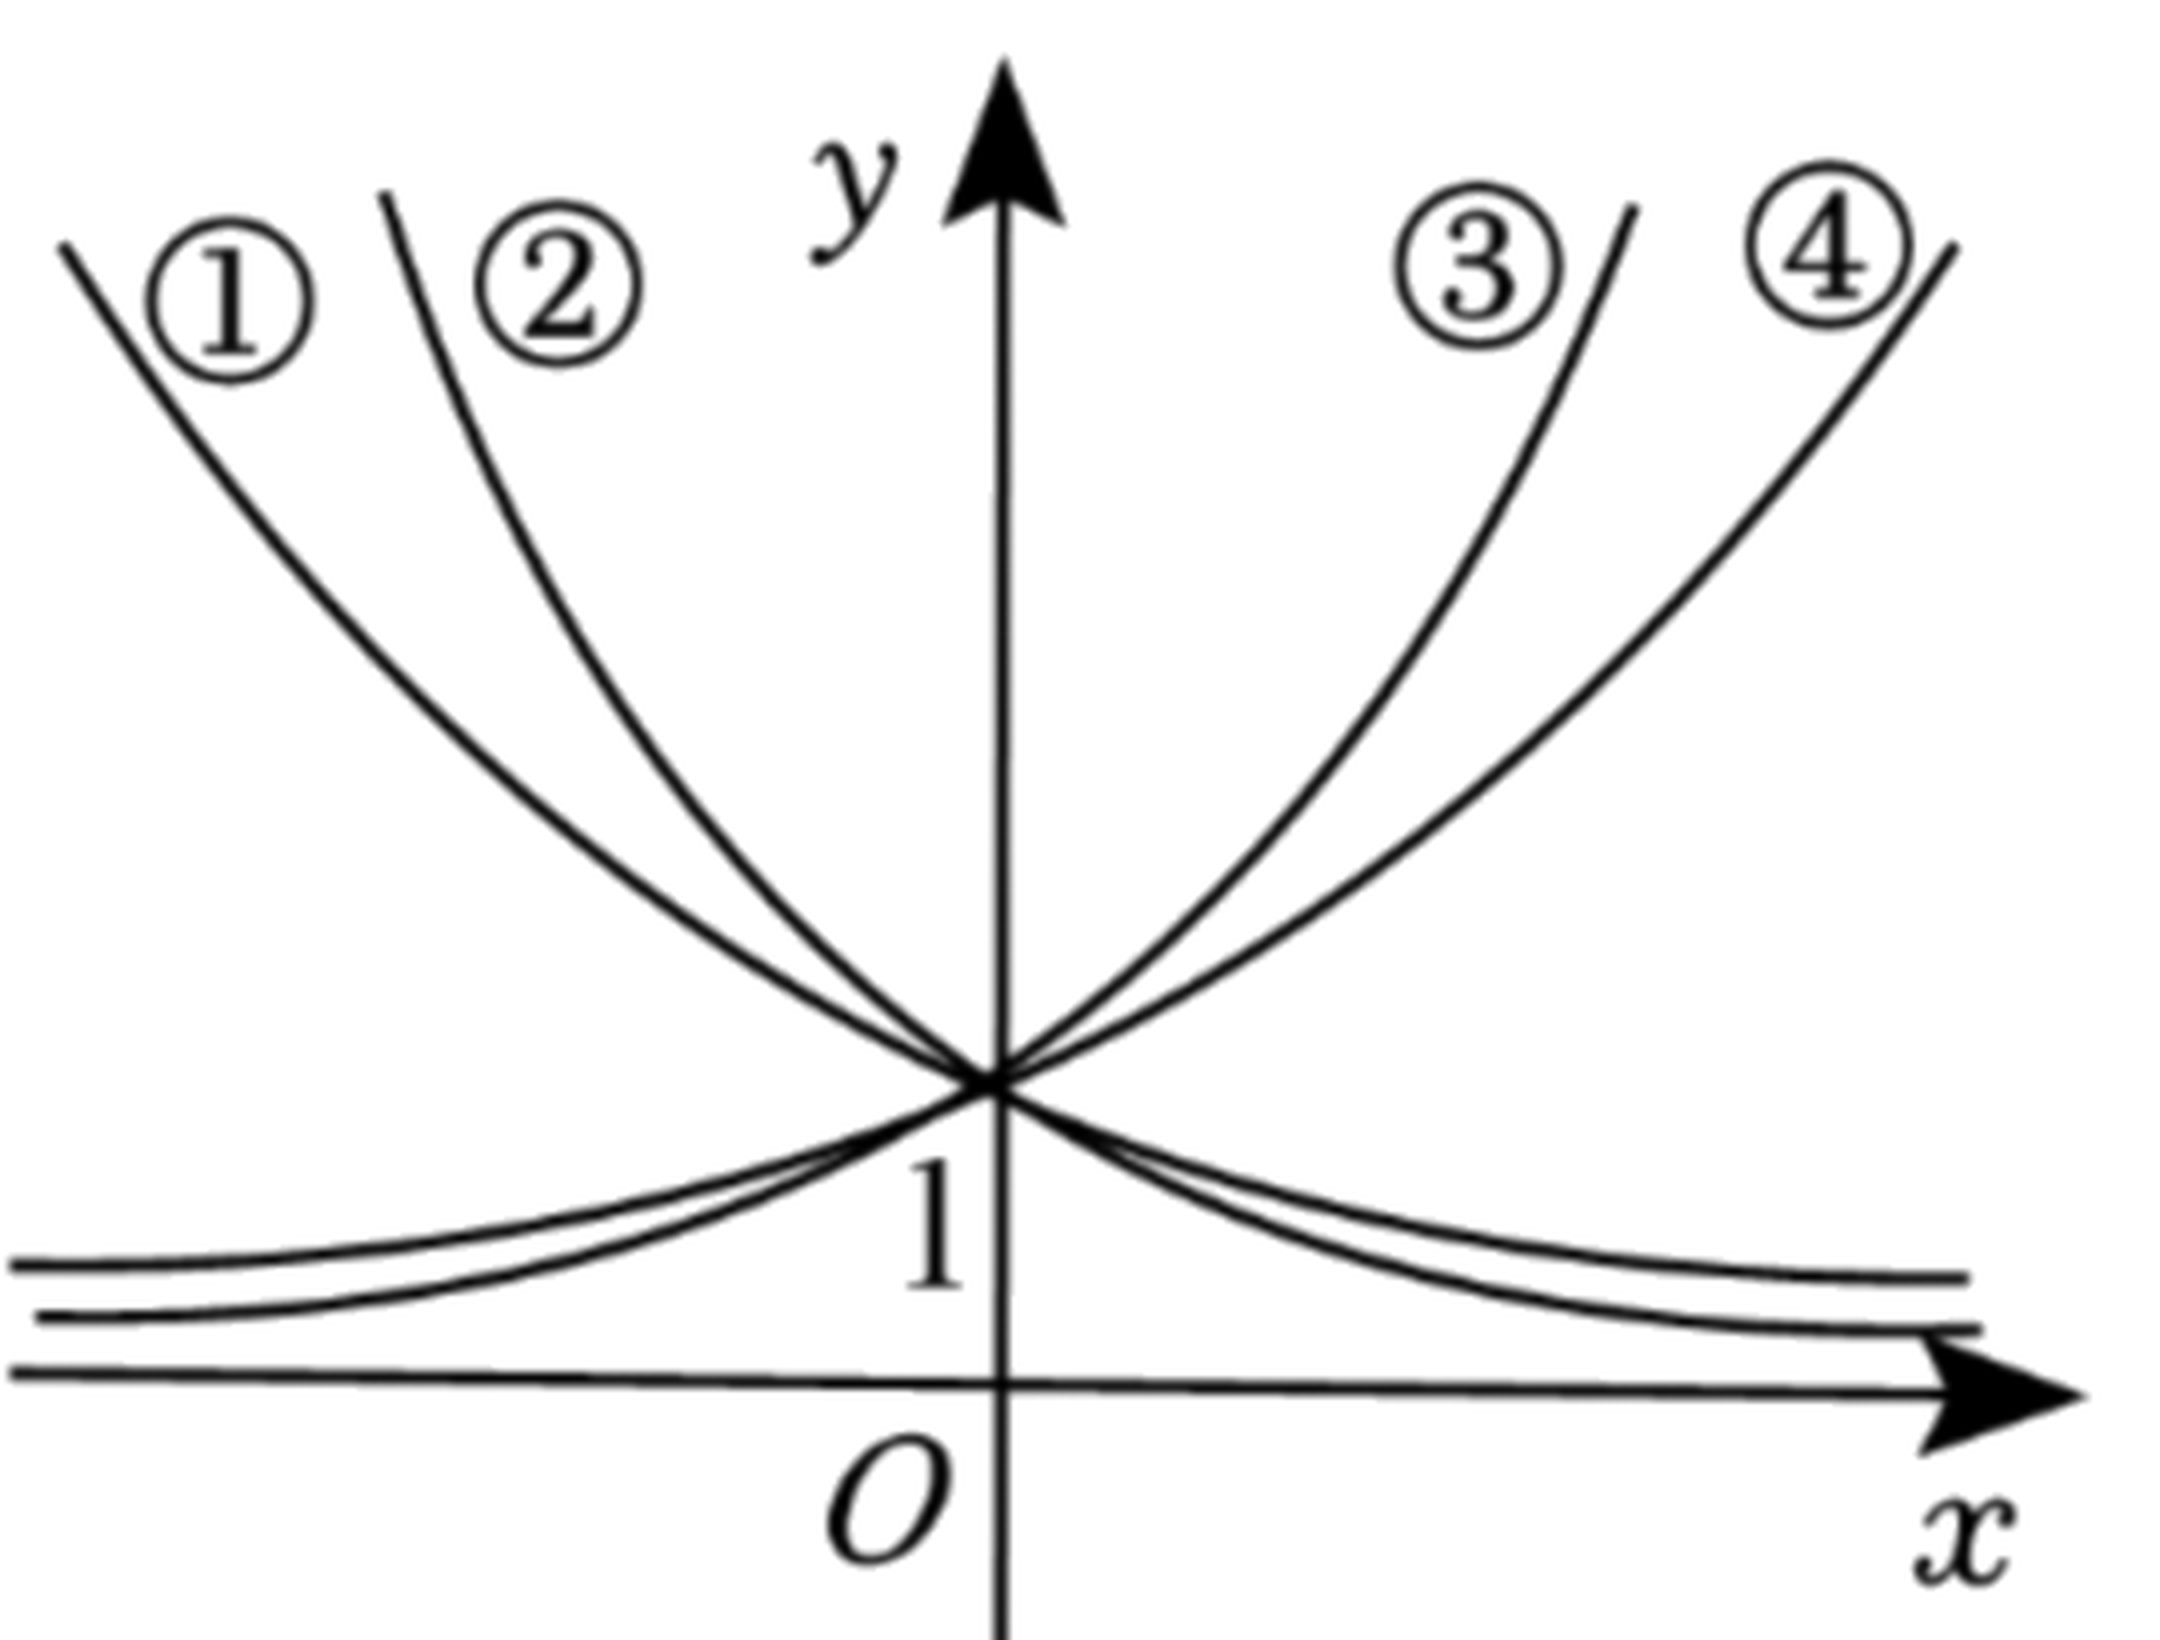
\includegraphics[width=0.40\textwidth]{figures/gao148_q15.png}
\end{center}

\ifanswer
\solbegin
\step{由函数图象得函数① $y=a^x$；② $y=b^x$ 为减函数，且 $x=1$ 时，$b^1<a^1$，}
\step{所以 $0<b<a<1$，}
\step{由函数图象得函数③ $y=c^x$；④ $y=d^x$ 为增函数，且 $x=1$ 时，$c^1>d^1$，}
\step{所以 $c>d>1$，}
\step{所以 $b<a<d<c$. 故选 $B$.}
\solend
\fi

% === Q16 ===：题目配图（关于 y 轴对称的幂函数曲线，三版都出），\needvspace 守卫放 \item 之前；$p$、$q\in\Z$；"图象"照录；解析 2 行
\needvspace{8cm}
\item 已知幂函数 $y=x^{\frac{p}{q}}$（$p$、$q\in\Z$ 且 $p$、$q$ 互质）的图象关于 $y$ 轴对称，如图所示，则\mbox{（\quad）}

\keepwithprev
A. $p$、$q$ 均为奇数，且 $\dfrac{p}{q}>0$\qquad\qquad B. $q$ 为偶数，$p$ 为奇数，且 $\dfrac{p}{q}<0$

C. $q$ 为奇数，$p$ 为偶数，且 $\dfrac{p}{q}>0$\qquad\qquad D. $q$ 为奇数，$p$ 为偶数，且 $\dfrac{p}{q}<0$

\begin{center}
% 关于 y 轴对称的幂函数曲线图取 04 页右下，去粉色水印、去色、4× LANCZOS 放大；三版都出
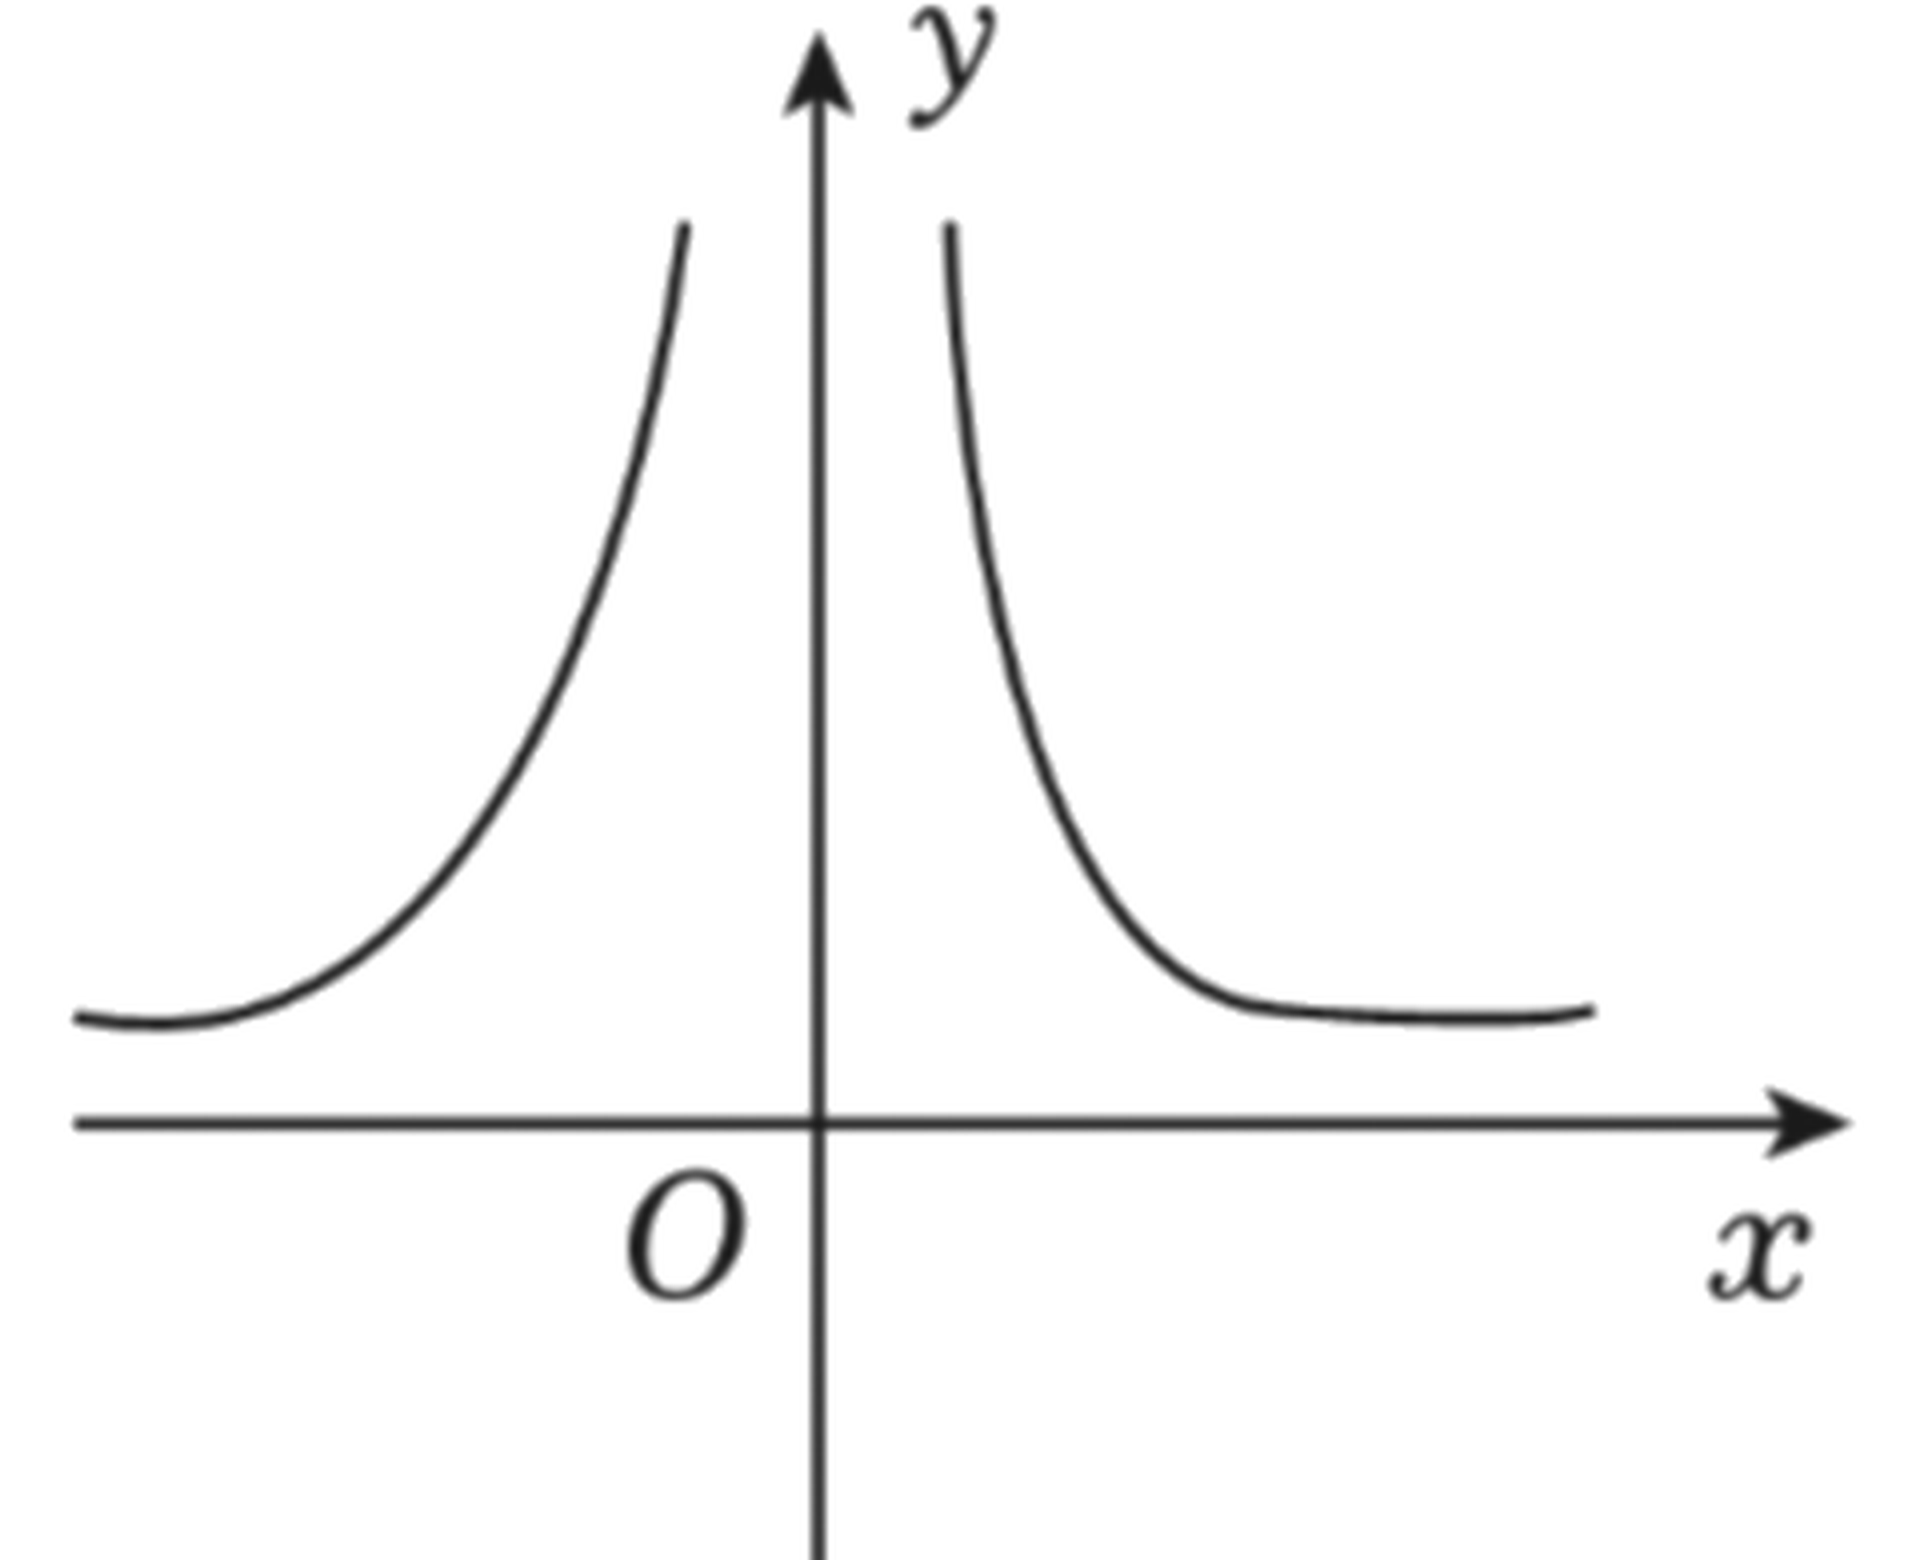
\includegraphics[width=0.36\textwidth]{figures/gao148_q16.png}
\end{center}

\ifanswer
\solbegin
\step{因为函数为偶函数，所以 $p$ 为偶数，且由图象形状判定 $\dfrac{p}{q}<0$.}
\step{又 $p$、$q$ 互质，所以 $q$ 为奇数. 故选 $D$.}
\solend
\fi

\end{enumerate}

\bigsec{三、解答题}

\begin{enumerate}
\setcounter{enumi}{16}

% === Q17 ===：\overline{B}／\varnothing／\R／\mid 逐处照录；解析 8 行
\item 已知集合 $A=\left\{x\mid \dfrac{5}{2x+1}>1\right\}$，$B=\{x\mid x^2+(a+3)x+3a<0,a\in\R\}$.

(1) 求 $A$.

(2) 若全集 $U=\R$，且 $A\cap\overline{B}=\varnothing$，求实数 $a$ 的取值范围.

\ifanswer
\solbegin
\step{(1) $\dfrac{5}{2x+1}>1$，即 $\dfrac{5}{2x+1}-1>0$，即 $\dfrac{4-2x}{2x+1}>0$，即 $(2x+1)(x-2)<0$，}
\step{解得 $-\dfrac{1}{2}<x<2$，所以 $A=\left(-\dfrac{1}{2},2\right)$；}
\step{(2) $x^2+(a+3)x+3a<0$，即 $(x+3)(x+a)<0$，}
\step{全集 $U=\R$，且 $A\cap\overline{B}=\varnothing$，}
\step{当 $a<3$ 时，解得 $-3<x<-a$，则 $\overline{B}=(-\infty,-3)\cup(-a,+\infty)$，}
\step{此时 $-a\geqslant2$，解得 $a\leqslant-2$，}
\step{当 $a\geqslant3$ 时，不满足 $A\cap\overline{B}=\varnothing$，}
\step{故实数 $a$ 的取值范围是 $(-\infty,-2]$.}
\solend
\fi

% === Q18 ===：cases 块整体算一个印刷行；解析 6 行
\item 已知幂函数经过点 $(2,4)$.

(1) 当 $x=\dfrac{1}{2}$ 时，求函数的值；

(2) 是否存在实数 $m$、$n$，使得该函数在区间 $[m,n]$ 上最小值为 $6m-8$，最大值为 $6n-8$？若存在，求出 $m$、$n$ 的值，若不存在，请说明理由.

\ifanswer
\solbegin
\step{(1) 设幂函数的解析式是 $y=x^\alpha$，则 $2^\alpha=4$，解得 $\alpha=2$，}
\step{故 $f(x)=x^2$，$f\left(\dfrac{1}{2}\right)=\dfrac{1}{4}$；}
\step{(2) 因为 $f(x)\geqslant0$，所以 $6m-8\geqslant0$，$m\geqslant\dfrac{4}{3}$，}
\step{由函数 $f(x)$ 在 $(0,+\infty)$ 严格增，得函数 $f(x)$ 在 $(m,n)$ 严格增，}
\step{所以 $\begin{cases}f(m)=6m-8\\f(n)=6n-8\end{cases}$ 且 $m<n$，解得 $m=2$，$n=4$，}
\step{故存在 $m=2$，$n=4$ 满足题意.}
\solend
\fi

% === Q19 ===：7 处评分档照 高一54／64 成例排 \dots\dots N 分；判别式高 \Delta；解析 9 行
\item 已知方程 $x^2+6mx+9m-2=0$，且 $x_1,x_2$ 是方程的两个不同的实数根.

(1) 若 $m=1$，求 $\dfrac{1}{x_1}+\dfrac{1}{x_2}$ 的值；

(2) 若 $m\in\R$，且 $x_1^2+x_2^2<4$，求 $m$ 取值范围.

\ifanswer
\solbegin
\step{(1) 当 $m=1$ 时，方程为 $x^2+6x+7=0$，\dots\dots1 分}
\step{则 $x_1+x_2=-6,x_1\cdot x_2=7$，\dots\dots2 分}
\step{$\dfrac{1}{x_1}+\dfrac{1}{x_2}=\dfrac{x_1+x_2}{x_1\cdot x_2}=-\dfrac{6}{7}$\dots\dots3 分}
\step{(2) $x_1+x_2=-6m,x_1\cdot x_2=9m-2$\dots\dots2 分}
\step{因为 $x_1^2+x_2^2=(x_1+x_2)^2-2x_1\cdot x_2$，所以 $(x_1+x_2)^2-2x_1\cdot x_2<4$，}
\step{所以 $36m^2-2(9m-2)<4$，解得 $0<m<\dfrac{1}{2}$\dots\dots2 分}
\step{又因为方程有两个不同的根，所以 $\Delta=36m^2-4(9m-2)>0$，}% 判别式原卷印等腰偏高粗三角 $\Delta$，照录（放大 07 页 q19_delta3.png／diag_band_q19.png 确认）
\step{解得 $m<\dfrac{1}{3}$ 或 $m>\dfrac{2}{3}$\dots\dots2 分}
\step{所以 $0<m<\dfrac{1}{3}$\dots\dots2 分}
\solend
\fi

% === Q20 ===：题目配图（矩形蔬菜温室，三版都出），\needvspace 守卫放 \item 之前；单位 \mathrm{m}／\mathrm{m}^2；解析 10 行
\needvspace{8cm}
\item 某村计划建造一个室内面积为 $600\mathrm{m}^2$ 的矩形蔬菜温室，在室内，沿左、右两侧与后侧内墙各保留 $2\mathrm{m}$ 宽的通道，沿前侧内墙保留 $4\mathrm{m}$ 宽的空地.

\begin{center}
% 矩形蔬菜温室示意图取 07 页右侧，去粉色水印、去色、4× LANCZOS 放大；三版都出
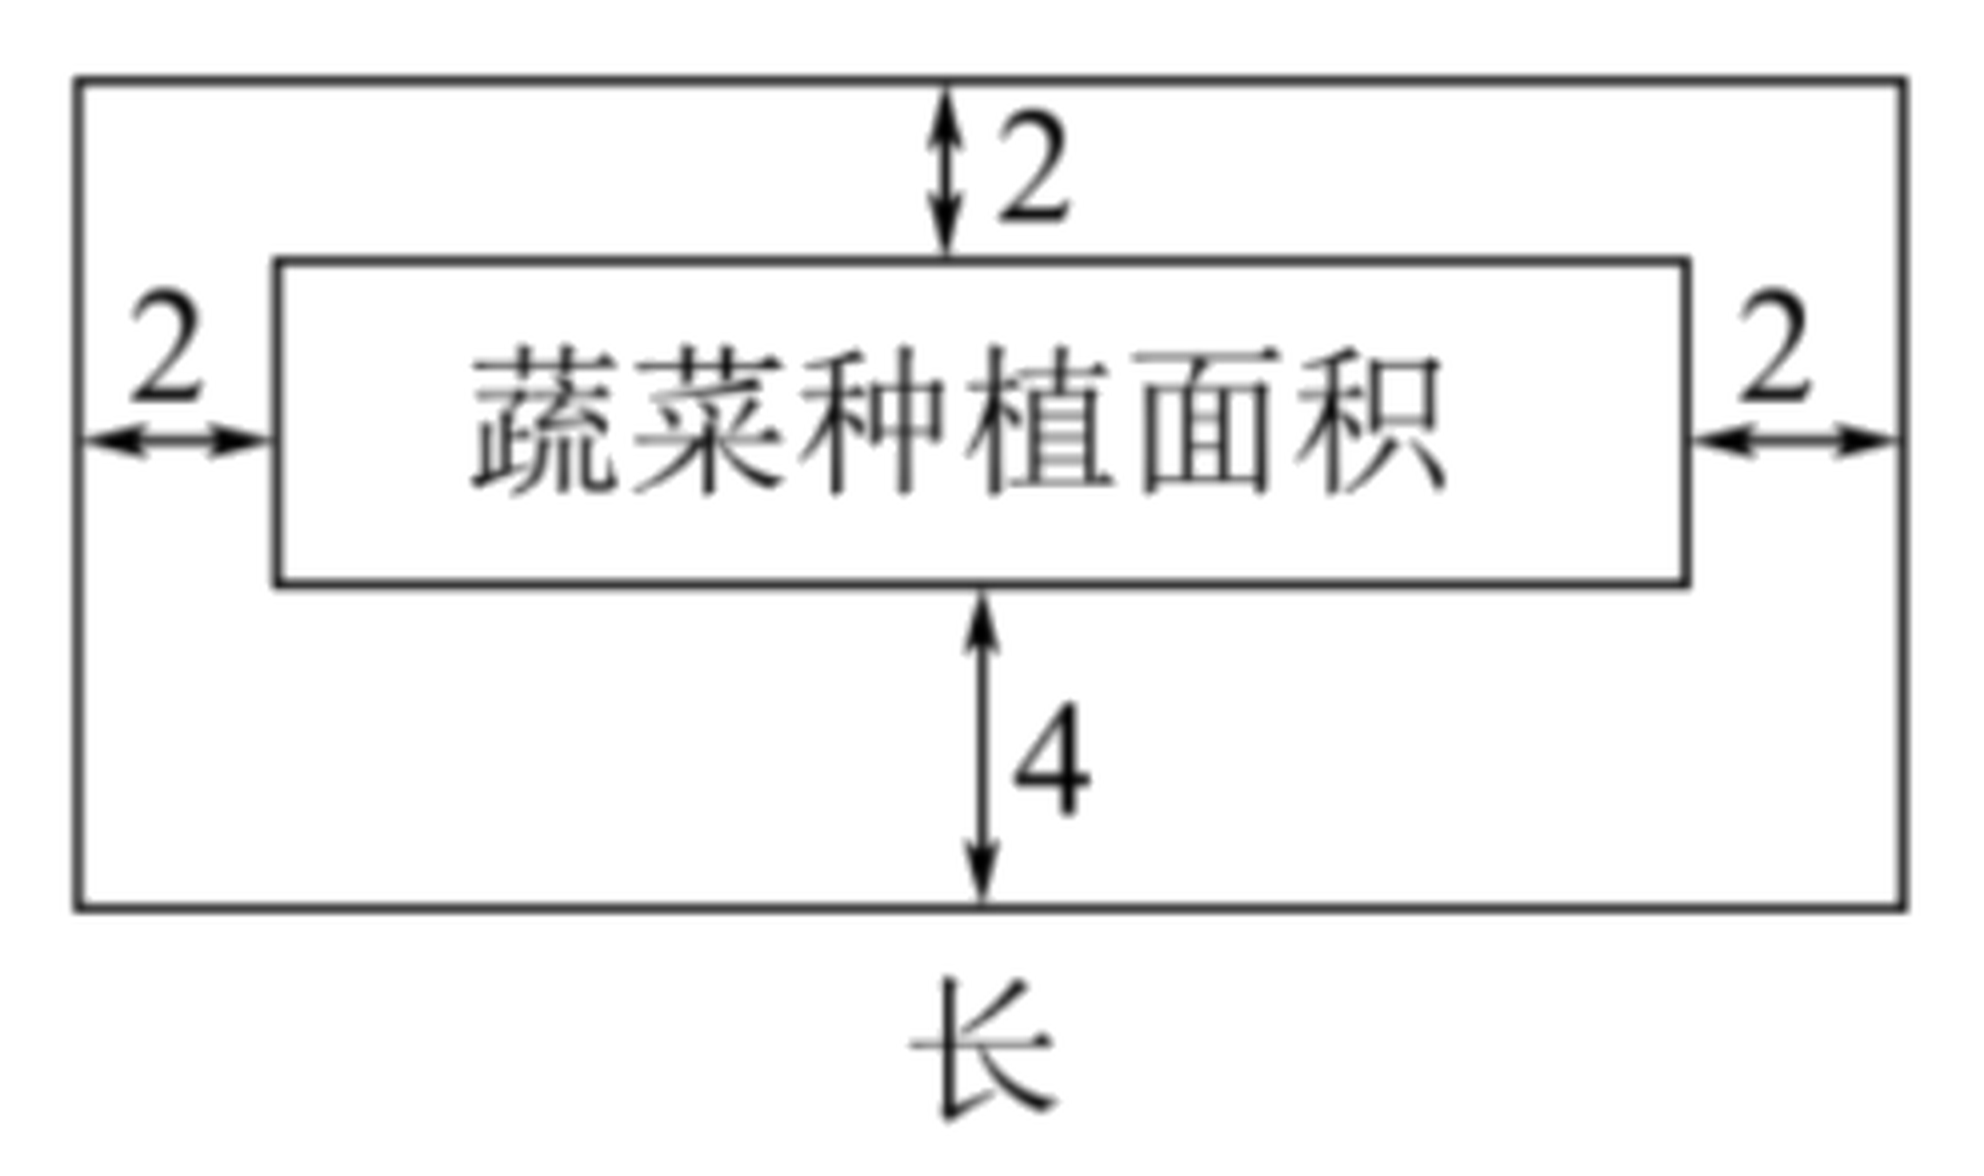
\includegraphics[width=0.45\textwidth]{figures/gao148_q20.png}
\end{center}

(1) 写出蔬菜的种植面积关于矩形温室的长之间的关系式.

(2) 当矩形温室的边长各为多少时，蔬菜的种植面积最大？最大种植面积是多少？

\ifanswer
\solbegin
\step{(1) 设蔬菜的种植面积为 $y\mathrm{m}^2$，矩形温室的长为 $x\mathrm{m}$，}
\step{则矩形温室的宽为 $\dfrac{600}{x}\mathrm{m}$，}
\step{种植蔬菜矩形的长为 $(x-4)\mathrm{m}$，宽为 $\left(\dfrac{600}{x}-6\right)\mathrm{m}$，}
\step{所以 $y=(x-4)\left(\dfrac{600}{x}-6\right)(4<x<100)$；}
\step{(2) 因为 $y=(x-4)\left(\dfrac{600}{x}-6\right)=624-\left(6x+\dfrac{2400}{x}\right)$，}
\step{因为 $6x+\dfrac{2400}{x}\geqslant2\sqrt{6x\cdot\dfrac{2400}{x}}=240$，}
\step{当且仅当 $6x=\dfrac{2400}{x}$，即 $x=20$ 时取等号，}
\step{所以 $y=624-\left(6x+\dfrac{2400}{x}\right)\leqslant624-240=384$.}
\step{即当矩形温室的一边长为 $20\mathrm{m}$，另一边长为 $30\mathrm{m}$ 时，}
\step{蔬菜的种植面积最大，最大为 $384\mathrm{m}^2$.}
\solend
\fi

% === Q21 ===：3 问、cases 块整体算一个印刷行；判别式高 \Delta；解析 19 行（末行续 09 页）
\item 二次函数 $f(x)=ax^2+bx+c$ 满足对任意的 $x\in\R$，$x-1\leqslant f(x)\leqslant x^2-x$ 恒成立.

(1) 求证：$f(1)$ 为定值；

(2) 若 $f(0)=-\dfrac{1}{4}$，求二次函数 $f(x)$ 的表达式；

(3) 求 $a+2b+5c$ 的取值范围.

\ifanswer
\solbegin
\step{(1) 对任意的 $x\in\R$，$x-1\leqslant f(x)\leqslant x^2-x$ 恒成立，则 $0\leqslant f(1)\leqslant0$，}
\step{所以 $f(1)=0$，为定值.}
\step{(2) 由(1)得 $a+b+c=f(1)=0$，由 $f(0)=-\dfrac{1}{4}$，得 $c=-\dfrac{1}{4}$，}
\step{则 $b=\dfrac{1}{4}-a$，$f(x)=ax^2+\left(\dfrac{1}{4}-a\right)x-\dfrac{1}{4}$，}
\step{不等式 $x-1\leqslant f(x)$ 可化为 $ax^2+\left(\dfrac{1}{4}-a\right)x-\dfrac{1}{4}\geqslant x-1$，}
\step{即 $ax^2-\left(a+\dfrac{3}{4}\right)x+\dfrac{3}{4}\geqslant0$，}
\step{一元二次不等式 $ax^2-\left(\dfrac{3}{4}+a\right)x+\dfrac{3}{4}\geqslant0$ 恒成立，则 $\begin{cases}a>0\\\Delta=\left(a+\dfrac{3}{4}\right)^2-3a\leqslant0\end{cases}$，}% 判别式原卷印等腰偏高粗三角 $\Delta$，照录（放大 08 页 q21_delta3.png／diag_band_q21.png 确认）
\step{解得 $a=\dfrac{3}{4}$，}
\step{此时 $f(x)=\dfrac{3}{4}x^2-\dfrac{1}{2}x-\dfrac{1}{4}$，$x^2-x-f(x)=\dfrac{1}{4}(x-1)^2\geqslant0$ 恒成立，}
\step{所以 $f(x)=\dfrac{3}{4}x^2-\dfrac{1}{2}x-\dfrac{1}{4}$.}
\step{(3) 由(1)得 $b=-a-c$，$f(x)=ax^2-(a+c)x+c=(ax-c)(x-1)$，}
\step{不等式 $x-1\leqslant f(x)$ 可化为 $(x-1)(ax-c-1)\geqslant0$，}
\step{一元二次不等式 $(x-1)(ax-c-1)\geqslant0$ 恒成立，则 $a>0$，}
\step{且方程 $(x-1)(ax-c-1)=0$ 有相等的实数根，因此 $c=a-1$，$a>0$，}
\step{不等式 $f(x)\leqslant x^2-x\Leftrightarrow(ax-c)(x-1)\leqslant x^2-x\Leftrightarrow(x-1)[(1-a)x+c]\geqslant0$，}
\step{同理 $1-a>0$，且方程 $(x-1)[(1-a)x+c]=0$ 有相等的实数根，}
\step{因此 $c=a-1$，$a<1$，从而 $c=a-1$，$b=1-2a$，$0<a<1$，}
\step{$a+2b+5c=a+2(1-2a)+5(a-1)=2a-3\in(-3,-1)$，}
\step{所以 $a+2b+5c$ 的取值范围是 $(-3,-1)$.}
\solend
\fi

\end{enumerate}

\end{document}
